\documentclass[12pt,twoside]{report}    

\usepackage[phd]{otagofront}   %% Use Otago page layout
\usepackage{natbib} 		%% author/year format in round brackets
\usepackage{graphicx}           %% jpg, gif, tiff, and pdf graphics
\usepackage{moreverb}           %% Verbatim Code Listings
\usepackage{amsmath}		%% More math commands
\usepackage{amssymb}		%% More math commands
\usepackage{amsthm}		%% More math commands
\usepackage{mathrsfs}		%% More math commands
\usepackage{color}		%% Handling colors
\usepackage{enumerate}          %% Fancy enumeration lists
\usepackage{lscape}
\usepackage{indentfirst}
%\usepackage{subfigure}
\usepackage{siunitx}
\usepackage{lscape}
\usepackage{subcaption}
\usepackage[toc,page]{appendix}
\usepackage[ruled,vlined,linesnumbered,resetcount,algochapter]{algorithm2e}

% % % % % % % % %  tikz package % % % % % % % %
\usepackage{tikz}
\usetikzlibrary{arrows.meta,calc,backgrounds}

\tikzset{
    right angle quadrant/.code={
        \pgfmathsetmacro\quadranta{{1,1,-1,-1}[#1-1]}     % Arrays for selecting quadrant
        \pgfmathsetmacro\quadrantb{{1,-1,-1,1}[#1-1]}},
    right angle quadrant=1, % Make sure it is set, even if not called explicitly
    right angle length/.code={\def\rightanglelength{#1}},   % Length of symbol
    right angle length=2ex, % Make sure it is set...
    right angle symbol/.style n args={3}{
        insert path={
            let \p0 = ($(#1)!(#3)!(#2)$) in     % Intersection
                let \p1 = ($(\p0)!\quadranta*\rightanglelength!(#3)$), % Point on base line
                \p2 = ($(\p0)!\quadrantb*\rightanglelength!(#2)$) in % Point on perpendicular line
                let \p3 = ($(\p1)+(\p2)-(\p0)$) in  % Corner point of symbol
            (\p1) -- (\p3) -- (\p2)
        }
    }
}
% % % % % % % % %  tikz package % % % % % % % %


%%%%%%%%%%%%%%%%%%%%%%%%%%%%%  New commands 

\newcommand{\BigO}[1]{{\rm O}\left(#1\right)}
\newcommand{\expo}{\,\mathrm{e}}
\newcommand{\cvar}{\,\mathrm{i}}
\newcommand{\besseli}{\mathrm{I}}
\newcommand{\besselk}{\mathrm{K}}
\newcommand{\bessely}{\mathrm{Y}}
\newcommand{\besselj}{\mathrm{J}}
\newcommand{\eg}{e.g.\ }
\newcommand{\elemvec}[2]{\big[#1\big]_{#2}}
\newcommand{\ud}[1]{\,\mathrm{d}#1}
\newcommand{\hPhi}{\widehat{\Phi}}
\newcommand{\diag}[1]{\text{diag}\left\{#1\right\}}
\renewcommand{\Re}{\operatorname{Re}}
\renewcommand{\Im}{\operatorname{Im}}

%\newcommand{\TODO}[1]{\textcolor{red}{\bf{[#1]}}}
%\newcommand{\EDITED}[1]{\textcolor{blue}{\bf{[#1]}}}

\newtheorem{lemma}{Lemma}
\newtheorem{theorem}{Theorem}
\newtheorem{corollary}{Corollary}

\newcommand{\E}{\mathrm{E}}
\newcommand{\Var}{\mathrm{Var}}
\newcommand{\Cov}{\mathrm{Cov}}
\newcommand{\Corr}{\mathrm{Corr}}
\newcommand{\tr}{\mathrm{tr}}
\newcommand{\iid}{\textrm{i.i.d.}}



%%%%%%%%%%%%%%%%%%%%%%%%%%% Front page info 

\title{Inference and Characterization of Planar Trajectories}
\author{Zhanglong Cao}
% %\date{30 August 2017}
\date{}
%%%%%%%%%%%%%%%%%%%%%%%%%%%%%% Extra info 

\fullname{Zhanglong Cao}
\department{Department of Mathematics and Statistics}
\dob{4 March 1984} %% date-of-birth
\address{46 St David Street, Dunedin, New Zealand}



%% Uncomment to just print up a few chapters.
%%
%\includeonly{}

\begin{document}


%% Put in titlepage and contents, etc...
\frontstuff

%% Set to one-and-a-half line-spacing
\linespread{1.3} \normalsize


\chapter{Introduction}\label{ChapterIntro}

%% % % %第一段: 提出并介绍这个问题
%The problem in the world I explore in this paper is....... 
%The reason why it is an important problem is......
%
%% % % %第二段:找出解决问题的视角
%The lends I adopt to explore this problem is.... it is a useful lens because..........
%
%% % % %第三段:描述解决问题的场景和发现Analyzing a dataset of xxxxxxxxxxx, 
%I reach the following findings.......
%
%% % % %第四段:介绍你的贡献
%This study contributes to.........

%Inference and Characterization of Planar Trajectories
%Inference and Characterization of Planar Trajectories
%Inference and Characterization of Planar Trajectories


\section{Background}


The Global Positioning System (abbreviated as GPS) is a space-based navigation system consisting of a network of 24 satellites placed in space in six different 12-hour orbital paths \cite{agrawal2015introduction}, so that at least five of them are in view from every point on the globe \cite{kaplan2005understanding} \cite{bajaj2002gps}. With these satellites, a GPS receiver sends geographic information to them and triangulate its location on the ground, such as longitude, latitude, and elevation. These receivers are using passive locating technology, by which they can receive signals without transmitting any data. It is perhaps the most widely publicized location-sensing system providing an excellent lateration framework for determining geographic positions \cite{hightower2001location}. Offered free of charge and accessible worldwide, GPS is used in plenty applications in military and general public, including aircraft tracking, vehicle navigation, robot localization, surveying, astronomy, and so on. 

For a moving vehicle, it is often mounted with a GPS unit that communicates with these satellites and records position, speed, and direction of traveling information. With this kind of information, a maneuvering target tracking system becomes available and useful. This tracking system can be used to reduce the cost by knowing in real-time the current location of a vehicle, such as a truck or a bus \cite{chadil2008real}, and also be useful for Intelligent Transportation System (ITS) \cite{mcdonald2006intelligent}. For instance, it can be used in probe cars to measure real-time traffic data to identify the congesting area. In particular, an orchardist is able to follow the trajectory and motion patterns of tractors, which are working on an orchard or vineyard, and monitor their working status with the tracking system. 



%It is suggested that the smoothing spline fitting through the measured values reflecting the movements is an alternative approach. Even though fitting a univariate local linear trend model using a Kalman filter is equivalent to fitting a cubic spline, see \cite{eubank2004simple}, \cite{durbin2012time}, the latter algorithm overcomes the current limitation and can approximate data points throughout the whole process. 
It is suggested that the smoothing spline fitting through the measured values reflecting the movements is an excellent approach, see \cite{eubank2004simple}, \cite{durbin2012time}. This algorithm can approximate data points throughout the whole process. 


\section{Smoothing Spline Based Reconstruction}


Starting from interpolation, the simplest way of connecting a set of sequences $(t_1,y_1),\ldots, (t_n,y_n)$ is by straight line segments. Known as piecewise linear interpolation. Apparently, sharp turnings occur at joint knots. A smooth path is expected and more common in real life application. A single polynomial function goes through the entire interval, such as B\'ezier curve, is not as flexible as a combination of several polynomials, each of which is defined on subintervals and joint at certain knots. This kind of piecewise polynomial interpolation is called a spline. 

The core idea of splines is to augment the vector of inputs $T$ with additional variables, then use linear models in this space of derived input features. Adding constraints to construct basis functions $h_i(t), i = 1, 2,\ldots, n$, a linear basis expansion in $T$ is represented as
\begin{equation*}
f(t)=\sum_{i=1}^n \theta_i h_i(t).
\end{equation*}
The key step of a spline interpolation is the choice of basis functions. Once the $h_i(t)$ have been determined, the models are linear in the variables space. 

Several kinds of splines were introduced by \cite{esl2009}. One of them is B-spline, short for basis spline, which is constructed from polynomial pieces and joint at knots. B-spline has a closed-form expression of positions and allows continuity between the curve segments and goes through the points smoothly with ignoring the outliers, see \eg \cite{komoriya1989trajectory}, \cite{ben2004geometric}. It is flexible and has minimal support with respect to a given degree, smoothness, and domain partition. Once the knots are given, it is easy to compute B-spline recursively for any desired degree of the polynomial \cite{de1978practical} \cite{cox1982practical}. Basic simplicity of the idea is explained in \cite{dierckx1995curve} and \cite{eilers1996flexible}. The attractive feature of B-spline is its flexibility for univariate regression. For example,  \cite{gasparetto2007new} is using a fifth-order B-spline to compose the overall trajectory with a set of paired data. Roughly speaking, every spline can be represented by B-spline basis. 

Another widely used spline is piecewise cubic spline, which is continuous on interval $[a,b]$ and its first and second derivatives are continues as well \cite{wolberg1988cubic}. For example, consider the model in the following form 
\begin{equation*}
f(t)=d_i(t-t_i)^3+c_i(t-t_i)^2+b_i(t-t_i)+a_i,
\end{equation*}
for given coefficients $d_i, c_i, b_i$ and $a_i$, where $t_i\leq t\leq t_{i+1}$, $i=1,2,\ldots,n$. $f$ is a cubic spline on $[a,b]$ if (\romannum{1}) on each intervals $f$ is a polynomial; (\romannum{2}) the polynomial pieces fit together at knots $t_i$ in such a way that $f$ itself, its first and second derivatives are continuous at each $t_i$. If the second and third derivatives of $f$ are zero at $a$ and $b$, $f$ is said to be a natural cubic spline and these conditions are called the \textit{natural boundary conditions} \cite{green1993nonparametric}. 


To find the best estimation $\hat{f}(t)$ going through observation $y_i$, $i=1,\ldots,n$, one can use regression methods returning the least residual sum of squares among all the sequences. Consider a model $y_i=f(t_i)+\varepsilon_i$ with random errors $\left\lbrace \varepsilon_i\right\rbrace_{i=1}^n \sim N(0,\sigma^2)$ in space $\mathit{C}^{(m)}[a,b]$, the classical parametric regression assumes that $f$ has the form of $f(t,\beta)$, which is known up to the data estimated parameters $\beta$ \cite{kim2004smoothing}. When $f(t,\beta)$ is linear in $\beta$, we will have a standard linear model. 


However, a parametric approach only captures features contained in the preconceived class of functions and increases model bias \cite{yao2005functional}. To avoid this, nonparametric methods have been developed. Rather than giving specified parameters, it is desired to reconstruct $f$ from the data $y(t_i)\equiv y_i$ itself  \cite{craven1978smoothing}. The estimates of polynomial smoothing splines appear as a solution to the following minimization problem: find $\hat{f} \in \mathit{C}^{(m)}[a,b]$ that minimizes the penalized residual sum of squares: 
\begin{equation}\label{introSmoothingOb}
\mbox{RSS}=\sum_{i=1}^{n}\left(  y_i-f(t_i)\right) ^2+\lambda\int_a^b \left(f^{(m)}\right)^2 dt
\end{equation}
for pre-specified value $\lambda(>0)$ \cite{aydin2012smoothing}. In the above equation, the first term is the residual sum squares controlling the lack of fit. The second term is the roughness penalty weighted by a smoothing parameter $\lambda$, which varies from $0$ to $+\infty$ and establishes a trade-off between interpolation and straight line in the following way: 
\begin{align*}\small 
\begin{cases}
\lambda = 0  & \mbox{$f$ can be any function that interpolates the data}\\
\lambda = +\infty & \mbox{the simple least squares line fit since no second derivative can be tolerated}\\
\end{cases}
\end{align*}\cite{esl2009}. 

Hence, the cost of the equation (\ref{introSmoothingOb}) is determined not only by its goodness-of-fit to the data quantified by the residual sum of squares but also by its roughness \cite{schwarz2012geodesy}. The motivation of the roughness penalty term is from a formalization of a mechanical device: if a thin piece of flexible wood, called a spline, is bent to the shape of the curve $g$, then the leading term in the strain energy is proportional to $\int f''^2$ \cite{green1993nonparametric}. 




%
%\subsection{Bayesian Estimation of Polynomial Smoothing Spline}
%
%Being bounded on a Hilbert space $C^{(m)}[0,1]$ with an inner product  $\langle f,g\rangle=\int_0^1fgdt$, \cite{wahba1978improper} showed that a Bayesian version of smoothing spline problem is to take a Gaussian process prior $f(t_i) = a_0+a_1t_i+\cdots + a_{m-1}t_i^{m-1} + x_i$, on $f$ with $x_i=X(t_i)$ being a zero mean Gaussian process whose $m$th derivative is scaled white noise, $i=1,\ldots,n$ \cite{speckman2003fully}. The extended Bayes estimates $f_\lambda$ with a "partially diffuse" prior is as exactly the same as spline solution. Some works have been done on discovering the relationship between nonparametric regression and Bayesian estimation. \cite{heckman1991minimax} shows that if $f$ the regression function $\E(y\mid f)$ has unknown prior distribution  $\mathbf{f}=(f(t_1),\ldots,f(t_n))^\top$ lying in a known class of $\Omega$, then the maximum is taken over all priors in $\Omega$ and the minimum is taken over linear estimator of $\mathbf{f}$. \cite{branson2017nonparametric} propose a Gaussian process regression method that acts as a Bayesian analog to local linear regression for sharp regression discontinuity designs. It is no doubt that one of the attractive features of the Bayesian approach is that, in principle, one can solve virtually any statistical decision or inference problem. Particularly, one can provide an accuracy assessment for $\hat{f}=\E (f\mid \mathbf{y})$ using posterior probability regions \cite{cox1993analysis}. 
%
%
%Based on the correspondence, \cite{craven1978smoothing} proposed an generalized cross-validation estimate for the minimizer $f_\lambda$. The estimate $\hat{\lambda}$ is the minimizer of the function where the trace of matrix $A(\lambda)$ in (\ref{crossvalidationmatrixA}) is incorporated. It is also able to establish an optimal convergence property for their estimator when the number of observations in a fixed interval tends to infinity \cite{wecker1983signal}. A high efficient algorithm to optimize generalized cross-validation and generalized maximum likelihood scores with multiple smoothing parameters via the Newton method was proposed by \cite{gu1991minimizing}. This algorithm can also be applied to the maximum likelihood and the restricted maximum likelihood estimation. The behavior of the optimal regularization parameter in the method of regularization was investigated by \cite{wahba1990optimal}. 
%



%\section{Parameter Selection}
\section{Cross-Validation Parameter Selection}

As discussed in the previous section, the determination of an optimal smoothing parameter $\lambda$ in the interval $(0,+\infty)$ was found to be an underlying complication and the fundamental idea of nonparametric smoothing is to let the data choose the amount of smoothness, which consequently decides the model complexity \cite{gu1998model}. Various studies for selecting an appropriate smoothing parameter are developed and compared in literatures. Most of these methods are focusing on data driven criteria, such as cross-validation (CV), generalized cross-validation (GCV) \cite{craven1978smoothing} and generalized maximum likelihood (GML) \cite{wahba1985comparison} and recently developed methods, such as improved Akaike information criterion (AIC) \cite{hurvich1998smoothing}, exact risk approaches \cite{wand1997exact} and so on. See \eg \cite{craven1978smoothing}, \cite{hardle1988far}, \cite{hardle1990applied}, \cite{wahba1990spline},  \cite{green1993nonparametric}, \cite{cantoni2001resistant} \cite{aydin2013smoothing}.  


%\subsection*{Cross-Validation}

A classical parameter selection method is \textit{cross-validation} (CV). The idea behind this method can be traced back to 1930s \cite{larson1931shrinkage}. Because in most applications, only a limited amount of data is available. Thus, an idea is to split this dataset into two subgroups, one of which is used for training the model and the other one is used to evaluate its statistical performance. The sample used in evaluation is considered as "new data" as long as data are \iid. 

A single data split yields a validation estimate of the risk and averaging over several splits yields a cross-validation estimate \cite{arlot2010survey}. Because of the assumption that data are identically distributed, and training and validation samples are independent, CV methods are widely used in parameter selection and model evaluation. 


For example, a $k$-fold CV splits the data into $k$ roughly equal-sized parts. For the $k$th part, we fit the model to the other $k-1$ parts
of the data, and calculate the prediction error of the fitted model when
predicting the $k$th part of the data. A detailed procedure is given by \cite{wahba1975completely}: suppose we have $n$ paired data $(t_1,y_1), \ldots, (t_n,y_n)$. Run a $k$-fold CV according to the following Algorithm \ref{kfoldCV}. 
\begin{algorithm}[h]
\SetAlgoLined 
%\KwResutt{Write here the resutt }
Initialization: Remove the first data $t_1$ and last date $t_n$ from the dataset. \\
Split the rest data $t_2,\ldots,t_{n-1}$ into $k$ groups by: $ \mbox{Group k} : t_{k+1}, t_{2k+1}, \cdots$ \\
Guess a value $\lambda^*$. \\
\While{CV score is not optimized}{
\For{$i=1,\ldots,k$}{ \label{kfoldCV01}
Delete the $i$th group of data. Fit a smoothing spline to the first data $(t_1,y_1)$, the rest $k-1$ groups of dataset and the last data $(t_n,y_n)$ with $\lambda^*$.\\ 
Compute the sum of squared deviations $s_i$ of this smoothing spline from the deleted $i$th group data points. \\ 
}\label{kfoldCV02}
Add the sums of squared deviations from steps \ref{kfoldCV01} to \ref{kfoldCV02} and divide it by $k$ to achieve a cross-validation score of $\lambda^*$, that is $s=\frac{1}{k}\sum_{i=1}^{k}s_i$. \\ \label{kfoldCV03}
Vary  $\lambda$ systematically and repeat steps \ref{kfoldCV01} to \ref{kfoldCV03} until CV shows a minimum.
}
 \caption{$k$-fold cross-validation.}\label{kfoldCV}
\end{algorithm}
Mathematically, we denote the CV score as 
\begin{equation*}
\mbox{CV}(\hat{f},\lambda) = \frac{1}{n}\sum_i^n \left( y_i -\hat{f}^{-k(i)}(t_i,\lambda) \right)^2,
\end{equation*}
where $\hat{f}^{(-k)}(t)$ denotes the fitted function computed with the $k$th part of the data removed. Typical choices for $k$ are 5 and 10 \cite{esl2009}.  The function $\mbox{CV}(\hat{f},\lambda)$ provides an estimate of the test error curve, and the tuning parameter $\lambda$ that minimizes it will be the optimal solution. 

A special case of $k$-fold CV is setting $k=n$, which is known as leave-one-out CV. In this scenario, the CV function takes each of the data out and calculate the errors of $\hat{f}^{(-i)}$ from the remaining $n-1$ points. In fact, with the property that taking one point out does not affect the estimation, the fitting of a smoothing spline allows us to implement CV methods without hesitation. 

As an improvement of CV, the GCV algorithm was proposed to calculate the trace of the estimation matrix $A(\lambda)$ instead of calculating individual elements for linear fitting under squared error loss, in which way it provides further computational savings. Suppose we have a solution $\hat{f}=A(\lambda)y$ with a given $\lambda$, for many linear fittings, the CV score is 
\begin{equation*}
\mbox{CV} = \frac{1}{n}\sum_{i=1}^{n} \left( y_i - \hat{f}^{(-i)}(t_i)\right)^2 = \frac{1}{n} \sum_{i=1}^{n}\left( \frac{y_i-\hat{f}(t_i)}{1-A_{ii}}  \right)^2, 
\end{equation*}
where $A_{ii}$ is the $i$th diagonal element of $A(\lambda)$. Then, the GCV approximation score is 
\begin{equation*}
\mbox{GCV} =\frac{1}{n} \sum_{i=1}^{n}\left( \frac{y_i-\hat{f}(t_i)}{1-\tr(A)/n}  \right)^2.
\end{equation*}
In smoothing problems, GCV can also alleviate the tendency of cross-validation to under-smooth \cite{esl2009}. 


%Almost every technique found in the scientific literature on the reconstruction and trajectory planning problem is based on the optimization of some parameters or some objective function, such as equation (\ref{introSmoothingOb}), \cite{gasparetto2007new}. The most significant optimality criteria are: 
%\begin{itemize}
%\item[1] minimum execution time,
%\item[2] minimum energy (or actuator effort),
%\item[3] minimum jerk.
%\end{itemize}
%Besides the aforementioned approaches, some hybrid optimality criteria have also been proposed (e.g. time energy optimal trajectory planning).
%


Rather than $\lambda$ being constant, a new challenge is posed that the smoothing parameter becomes a function $\lambda(t)$ and is varying in domains. The structure of this penalty function controls the complexity of each domain and the whole final model.  \cite{donoho1995wavelet} introduced adaptive splines and a method to calculate piecewise parameters and \cite{liu2010data} give an improved formula for this method. They proposed an approximation to the penalty function with an indicator and extended the generalized likelihood to the adaptive smoothing spline. This will be another interesting research topic. 


%Craven and Wahba [5], Hardle [8], Hardle, Hall and Marron
%[9], Wahba [26], Hurvich, et al. [11], Eubank [6], Lee and Solo [17], Hastie and Tibshirani
%[10], Schimek [22], Cantoni and Ronchetti [4], Ruppert, Wand and Carroll [21], Lee [15, 16],
%and Kou [12] supplement on the selection of the smoothing parameter


%\textbf{Temporally put here }Due to the noise generated from observation units, one can use regression methods to find the best reconstruction returning the least sum square errors among all the sequences. Consider a regression model $y_i=f(t_i)+\epsilon_i$, where $a \leq t_1 < \cdots < t_n \leq b$ and $f \in \mathit{C}^2[a,b]$ is an unknown smooth function, $(\epsilon_i)_{i=1}^n \sim N(0,\sigma^2)$ are random errors. In a classical parametric regression, $f$ is assumed having the form $f(x,\beta)$, which is known up to the data estimated parameters $\beta$ \cite{kim2004smoothing}. When $f(x,\beta)$ is linear in $\beta$, we will have a standard linear model. 


%\subsection*{Improved AIC}
%
%The AIC, abbreviated for Akaike Information Criterion, is originally for parametric problems of model selection. 





\section{Bayesian Filtering}

Smoothing spline algorithms have several advantages in inferring and characterizing planar trajectories, particularly in reconstructing. However, subject to the property that smoothing splines require the solution of a global problem that involves the entire set of points to be interpolated, it might not be suitable for on-line estimation \cite{biagiotti2013online}. Therefore, it is time to use Bayesian filtering to implement instant/on-line estimation and prediction. 

The word \textit{filtering} refers to the methods for estimating the state of a time-varying system, which is indirectly observed through noisy measurements. A Bayes filter is a general probabilistic approach to infer an unknown probability density function recursively over time using incoming measurements and a mathematical process model. The concept \textit{optimal estimation} refers to some criteria that measure the optimality in specific sense \cite{anderson1979optimal}. For example, a posterior estimation of $\hat{x}_t\sim p(x_t\mid y_{1:t})$ that minimizes the loss function $J_t=\E\lbrack x_t-\hat{x}_t\rbrack^2$ for incorrect estimates, or least mean squared errors, maximum likelihood approximation and so on \cite{chen2003bayesian} \cite{sarkka2013bayesian}. Hence, an optimal \textit{Bayesian filtering} is using Bayesian way of formulating optimal filtering by meeting some statistical criteria. 

It is no doubt that in a conventional target tracking system, the most common method is the standard Kalman filter, which is a recursive solution to the discrete data linear filtering problem. 



\subsection*{Kalman Filter}

In a discrete-time linear system, the optimal Bayesian solution coincides with the least squares solution. The successful optimal one was given by \cite{kalman1960new}, the celebrated \textit{Kalman filter}. It is a set of mathematical equations that provides an efficient computational means to estimate the state of a process in a recursive way by minimizing the mean of the squared errors \cite{bishop2001introduction}. 

The Kalman filter recursively updates the estimated state by computing from the previous estimation and a new observation. In addition to eliminating the need for storing the entire past observed data, it is computationally more efficient than computing the estimate directly from the entire past observed data at each step of the filtering process \cite{haykin2001kalman}.  

A detailed Kalman filter and its may variants can be found in \cite{chen2003bayesian}, \cite{rhodes1971tutorial}, \cite{kailath1981lectures}, \cite{sorenson1985kalman}. And  \cite{tusell2011kalman} gives a review of some \textit{R} packages, which are used to fit data with Kalman filter methods. Besides, it is also shown that the Kalman filter can be derived within a Bayesian framework and reduces to a maximum posterior probability (MAP) solution, and can be easily extended to ML solution. See \cite{haykin2001kalman} and \cite{guzzi2016data}. 

Consider the following model 
\begin{align}\label{introKFmodel}
\begin{array}{cccccccccc}\cdots &\to &x_{t-1}&\to &x_{t}&\to &x_{t+1}&\to &\cdots &{\text{truth}}\\ &&\downarrow &&\downarrow &&\downarrow && &\\ \cdots&&y_{t-1}&&y_{t}&&y_{t+1}&&\cdots &{\text{observation}}\end{array}
 \end{align}
in which $x_t=F(x_{t-1})+\varepsilon_x$ is the true hidden state propagating through the transition matrix $F$ and $y_t=G(x_t)+\varepsilon_y$ is the observation measured by the measurement matrix $G$ of the system, where $\varepsilon$ indicates \iid noise in the model. 

To estimate the filtering state $x_t$ from $y_{1:t}=\left\lbrace y_1,\ldots,y_t\right\rbrace$, Bayesian wants to maximize the posterior $p(x_t\mid y_{1:t})$ by marginalizing out all the previous measurements. Given the joint distribution of $p(x_t,x_{t-1},y_{1:t})$, Kalman filter supposes the expectation $\hat{x}_{t-1}$ and its variance $S_{t-1}$ are known and passing through the system by $\hat{x}_t=F\hat{x}_{t-1}$ and $S_t=FS_{t-1}F^\top + Q_t$. Because of the log likelihood function is written as
$\ln p(x_t\mid y_{1:t}) \propto \frac{1}{2}(y_t-Gx_t)^2-\frac{1}{2}(x_t-\hat{x}_{t-1})^2$,
as a result, the solution is 
\begin{equation*}
\hat{x}_t = \left(G^\top R^{-1}G+S_{t-1}^{-1}\right)^{-1}\left( G^\top R_t^{-1}y_t+S_{t-1}^{-1}\hat{x}_{t-1} \right).
\end{equation*}
Additionally, by setting $S_t^{-1} = G^\top R_t^{-1}G+S_{t-1}^{-1}$, the recursive estimation of covariance matrix is $S_t = S_{t-1} - K_t GS_{t-1}$, 
and $K_t = S_{t-1} G^\top (R_t +GS_{t-1}G^\top)^{-1}$ is named Kalman gain matrix. Consequently, the recursive estimation is 
\begin{equation}\label{KalmanEstimation}
\hat{x}_t = \hat{x}_{t-1}+K_t(y_t-G\hat{x}_{t-1}).
\end{equation}

Furthermore, compared with filtering distribution $p(x_t\mid y_{1:t})$, the prediction distribution is trying to find an $n$-steps later distribution $p(x_{t+n}\mid y_{1:t})$ from the current state, and the smoothing distribution is to find the distribution $p(x_k\mid y_{1:t})$ of a specific state $x_k$ in the past for any $k$, where $1<k<t$. 

Kalman filter has a limitation that it does not apply to general non-linear model and non-Gaussian distributions. For a non-linear system, one can use the extended Kalman filter (EKF), which is widely used for solving nonlinear state estimation applications \cite{gelb1974applied}, \cite{bar1993estimation}. The EKF uses Taylor expansion to construct linear approximations of nonlinear functions, therefore, the state transition $f$ and observation $g$ do not have to be linear but to be differentiable. However, in the EKF process, these approximations can introduce large errors in the true posterior mean and covariance of the transformed (Gaussian) random variable \cite{wan2000unscented}. 

Alternatively, the Unscented Kalman Filter (UKF) is a derivative-free method \cite{julier1997new}, \cite{wan2000unscented}, \cite{gyorgy2014unscented}. It is using the Kalman filter to create a normal distribution that approximates the result of a non-linear transformation numerically by seeing what happens to a few deliberately chosen points. The unscented transform is used to recursively estimating the equation (\ref{KalmanEstimation}), where the state random variable is redefined as the concatenation of the original state and noise variables. By contrast, Kalman filter does not require numerical approximations. 

The performances of EKF and UKF are compared in a few references regarding to different kinds of aspects, such as \cite{chandrasekar2007comparison}, \cite{laviola2003comparison}, \cite{st2004comparison}. There is not an overall conclusion that which one performs better. 


Limited to its property, Kalman filter is tied up for a dynamic system, where the parameters and noise variances are unknown. In some dynamic systems, the variances are obtained based on the system identification algorithm, correlation method, and least squares fusion criterion. To solve this issue, a self-tuning weighted measurement fusion Kalman filter is presented in \cite{ran2010self}. Likewise, a new adaptive Kalman filter will be another choice \cite{oussalah2001adaptive}. 


However, when the target maneuver occurs, Kalman filtering accuracy will be reduced or even diverged due to the model mismatch and noise characteristics that cannot be known exactly \cite{liu2014filtering}. Additionally, Kalman filter based methods require the state vector contains pre-specified coefficients during the whole approximation procedure and are within the bounded definition range determined at the beginning \cite{jauch2017recursive}. 

A more generic algorithm is introduced in the following section. 


\subsection*{Monte Carlo Filter}

\textit{Monte Carlo filter}, \cite{chen2003bayesian},  is a class of Monte Carlo approaches. The power of these approaches is that they can numerically and efficiently handle integration and optimization problems. 

The important advantage of Monte Carlo is that a large number of posterior moments can be estimated at a reasonable computational effort and that estimates of the numerical accuracy of these results are obtained in a simple way \cite{kloek1978bayesian}. \textit{Sequential Monte Carlo} method is using Monte Carlo approaches to estimate and to compute recursively. One of the attractive merits is in the fact that they allow on-line estimation by combining the powerful Monte Carlo sampling methods with Bayesian inference at an expense of reasonable computational cost \cite{chen2003bayesian}. 

For example, consider the model (\ref{introKFmodel}) with parameter $\theta$. The likelihood approximation is $p(y_t\mid y_{1:t-1},\theta)$ and can be written by
\begin{equation*}
p(y_t\mid y_{1:t-1},\theta) = \int p(y_t\mid x_t,\theta)p(x_t\mid y_{1:t-1},\theta) dx_t = \E \lbrack p(y_t\mid x_t,\theta)\rbrack.
\end{equation*}
The standard Monte Carlo algorithm is trying to compute the integration by drawing $N$ independent samples $x_t^{(i)}$ from $p(x_t\mid y_{1:t-1},\theta)$ at first and then, by adding them up, to approximate the integration for large $N$ in the following way 
\begin{equation*}
\E\left[p(y_t\mid x_t,\theta)\right]\approx \frac{1}{N}\sum_i p(y_t\mid x_t^{(i)},\theta), 
\end{equation*}
\cite{kalos2008monte}.

In terms of getting good samples of $x_t^{(i)}$, which can be used for representing $p(y_t\mid x_t^{(i)},\theta)$, an importance sampling method was devised. The idea of this method is by assigning weights $W_t^{(i)}$ to samples, the most important ones are evaluated for computing the integral. Further, sequential importance sampling (SIS) allows a sequential update of the importance weights by 
\begin{equation*}
W_t^{(i)} \propto W_{t-1}^{(i)} \frac{ p\left(y_t \mid x_t^{(i)}\right) p\left(x_{t}^{(i)}\mid x_{t-1}^{(i)}\right) }{q\left(x_{t}^{(i)}\mid x_{t-1}^{(i)},y_{t}\right)}
\end{equation*}
with an appropriate chosen \textit{proposal distribution} $q(x_{t}\mid  x_{t-1},y_{t})$. It is also called \textit{importance density} or \textit{important function} \cite{chen2003bayesian}. 


Nevertheless, the SIS makes samples skewed that only a few samples have proper weights as time increases and most of them have small but positive weights. This phenomenon is often called \textit{weight degeneracy} or \textit{sample impoverishment} \cite{green1995reversible} \cite{berzuini1997dynamic}. 


Besides the SIS processes, a resampling step, also known as a selection step, is trying to eliminate the samples with small weights and duplicate the samples with large weights in a principled way \cite{rubin2004multiple}, \cite{tanner1987calculation}. This method is named \textit{sampling and importance resampling} SIR. Suppose samples with associated weights are $\left\lbrace x_t^{(i)},W_t^{(i)}\right\rbrace$, a resampling step is executed by generating new samples $\tilde{x}_t^{(i)}$ according to normalized weights $\tilde{W}_t^{(i)}$. It is pointed out that the resampling step does not prevent weights degeneracy but improve further calculation. 

The common feature of SIS and SIR is that both of these methods are based on importance sampling and updating samples weights recursively. The difference is that in SIR, the resampling step is always performed. Whereas in SIS, resampling is only taken when needed. 


The most successful application of importance sampling with resampling algorithm is \textit{Particle filter} (PF). PF randomly generates a cloud of points and push these points through the computation process. It is a recursive implementation of the Monte Carlo approaches \cite{doucet2009tutorial}. 


A generic PF firstly generates $N$ uniformly weighted random measurements $\left\lbrace x_{t-1}^{(i)},\frac{1}{N} \right\rbrace$ at time $t-1$. Once a new observation $y_t$ comes into the system, the weights will be updated recursively by involving the likelihood function $p(y_t\mid x_t^{(i)})$ and propagation function $p(x_t^{(i)}\mid x_{t-1}^{(i)})$. In fact, it is the SIS step. To monitor how bad is the weight degeneracy, a suggested measurement \textit{effective sample size} was introduced in \cite{kong1994sequential}. It is the reciprocal of the sum of squared weights in the form of 
\begin{equation*}
N_{\mbox{\footnotesize eff}} = \frac{1}{\sum_{i=1}^{N}\left(W_t^{(i)} \right)^2}. 
\end{equation*}
If the $N_{\mbox{\footnotesize eff}}$ is less than a predefined threshold, the resampling procedure is executed and the set of particles remains the same size $N$. 



However, the PF sampling and resampling methods may cause practical problems. Such as high weighted particles have been selected many times and lead to the loss of diversity. This problem is known as sample impoverishment, in which way the particles are not representative. The improvements of particle filter's performance have been devoted by \cite{carpenter1999improved}, \cite{godsill2001maximum}, \cite{stavropoulos2001improved}, \cite{smcmip2011}. 


Apparently, Bayesian filtering has become a broad topic involving many scientific areas that a comprehensive survey and detailed treatment seems crucial to cater the ever growing demands of understanding this important field for many novices, though it is noticed by the author that in the literature there exist a number of excellent tutorial papers on particle filters and Monte Carlo filters \cite{chen2003bayesian} \cite{doucet2000sequential} \cite{doucet2000rao} \cite{chen2012monte}.  
 



\section{Markov Chain Monte Carlo Methods}


Schemes exist to counteract sample impoverishment, which incurs in particle filter \cite{ristic2004beyond}. One approach is to consider the states for the particles to be predetermined by the forward filter and then to obtain the smoothed estimates by recalculating the particles' weights via a recursion from the final to the first time step \cite{godsill2000methodology}. Another approach is to use a \textit{Markov chain Monte Carlo} (MCMC) move step \cite{carlin1992monte}. MCMC refers to constructing Markov chains that move in the space of the unobserved quantity of interest and produces a sequence of dependent samples from the posterior distribution. After the chain has been run long enough, the sequence of visited states may be used as an approximation to the posterior distribution \cite{kokkala2016particle}. 


MCMC methods are a set of powerful stochastic algorithms that allow us to solve most of these Bayesian computational problems when the data are available in batches \cite{andrieu1999sequential}, \cite{green1995reversible}, \cite{andrieu2001model}. They are based on sampling from probability distributions based on a Markov chain. If samples are unable to be drawn directly from a distribution $\pi(x)$, we can construct a Markov chain of samples from another distribution $\hat{\pi}(x)$ that is equilibrium to $\pi(x)$. If the chain is long enough, these samples of the chain can be used as a basis for summarizing features of $\pi(x)$ of interest \cite{smith1993bayesian}. This is a crucial property. See \eg \cite{cappe2009inference} and \cite{liu2008monte} for details. 




\subsection*{Metropolis-Hastings Algorithm}

The \textit{Metropolis-Hastings} (MH) algorithm is an important class of MCMC algorithms \cite{smith1993bayesian} \cite{tierney1994markov} \cite{gilks1995markov}. Given essentially a probability distribution $\pi$ (the "target distribution"), MH algorithm provides a way to generate a Markov chain $x_1, x_2,\ldots, x_t$, who has the target distribution as a stationary distribution, for the uncertain parameters $x$ requiring only that this density can be calculated at $x$. Suppose that we can evaluate $\pi(x)$ for any $x$. The transition probabilities should satisfy the detailed balance condition
\begin{equation*}
\pi\left(x^{(t)}\right)q\left(x', x^{(t)}\right) = \pi\left(x'\right)q\left(x^{(t)}, x'\right),
\end{equation*}
which means that the transition from the current state $\pi\left(x^{\left(t\right)}\right)$ to the new state $\pi\left(x'\right)$ has the same probability as that 
from $\pi\left(x'\right)$ to $\pi\left(x^{\left(t\right)}\right)$. In sampling method, drawing $x_i$ first and then drawing $x_j$ should have the same probability as drawing $x_j$ and then drawing $x_i$. However, in most situations, the details balance condition is not satisfied. Therefore, a function $\alpha\left(x,y\right)$ is introduced for satisfying 
\begin{equation*}
\pi\left(x'\right)q\left(x', x^{\left(t\right)}\right)\alpha\left(x',x^{\left(t\right)}\right) = \pi\left(x^{\left(t\right)}\right)q\left(x^{\left(t\right)}, x'\right)\alpha\left(x^{\left(t\right)},x'\right).
\end{equation*}
In this way, a tentative new state $x'$ is generated from the proposal density $q\left(x';x^{\left(t\right)}\right)$ and it is then accepted or rejected according to acceptance probability 
\begin{equation}\label{IntroAccp}
\alpha=\frac{\pi\left(x'\right)}{\pi\left(x^{\left(t\right)}\right)}\frac{q\left(x^{\left(t\right)}, x'\right)}{q\left(x', x^{\left(t\right)}\right)}.
\end{equation}
If $\alpha \geq 1$, then the new state is accepted. Otherwise, the new state is accepted with probability $\alpha$.

A simple mechanic proposing algorithm is \textit{Random Walk Metropolis-Hastings} (RM MH). It is easy to implement and symmetric under the exchange of the initial and proposed points. 

Besides, modified Metropolis-Hastings algorithms, such as the delayed-rejection MH, multiple-try MH and reversible-jump MH algorithms have been studied by \cite{tierney1999some}, \cite{liu2000multiple} and \cite{green1995reversible}. 
 

%\subsection*{Gibbs Sampling Algorithm}
%
%\textit{Gibbs sampling}, also known as the heat bath method or "Glauber dynamics", was proposed by \cite{geman1984stochastic}. It has been proved particularly convenient for a range of applications in Bayesian statistics \cite{smith1993bayesian} \cite{mackay2003information}. Gibbs sampler is generating posterior samples conditionally on remaining variables fixed to their current values from a distribution that has at least two dimensions. For example, consider a general case that contains $N$ variables $x_t^{(1)},\ldots,x_t^{(N)}$ at time $t$. The samples for the next state $t+1$ will be 
%\begin{align*}
%x_{t+1}^{(1)}  &\sim \pi(x_1 \mid x_t^{(2)},x_t^{(3)},\ldots,x_t^{(N)}) \\
%x_{t+1}^{(2)}  &\sim \pi(x_2 \mid x_{t+1}^{(1)},x_t^{(3)},\ldots,x_t^{(N)}) \\
%&\vdots \\
%x_{t+1}^{(N)}  &\sim \pi(x_N \mid x_{t+1}^{(1)},x_{t+1}^{(2)},\ldots,x_{t+1}^{(N-1)})
%\end{align*}
%using the newly updated sample $x_{t+1}^{(i)}$. After one iteration, the new sequence $x_{t+1}^{(1)},\ldots,x_{t+1}^{(N)}$ is obtained. 
%
%Gibbs sampling can be viewed as one of Metropolis methods and meets the convergence property that the probability distribution of $x_t$ tends to $\pi(x)$ as $t\to\infty$, as long as $\pi(x)$ does not have pathological properties. Similarly to MH algorithms, some modified Gibbs sampler, such as single-site Gibbs sampling algorithm \cite{sorensen2007likelihood}, a blocked Gibbs sampling algorithm \cite{garcia1996multivariate} and hybrid Gibbs sampling algorithm \cite{mathew2012bayesian}, are well developed and applied in different applications \cite{gelfand1990illustration}. 



\subsection*{Adaptive MCMC Algorithm}


Metropolis-Hastings algorithm is widely used in statistical inference, to sample from complicated high-dimensional distributions. Typically, this algorithm has parameters that must be tuned in each new situation to obtain reasonable mixing times, such as the step size in a random walk Metropolis \cite{mahendran2012adaptive}. Tuning of associated parameters such as proposal variances is crucial to achieving efficient mixing, but can also be difficult. 

%It is introduced that Metropolis-Hastings algorithm draws samples from a target distribution $\pi(\cdot)$ by proposing $x'$ from $x^{(t)}$. Then calculate a probability to decide whether accept or reject it. The proposal distribution 

\textit{Adaptive MCMC} methods have been developed to automatically adjust these parameters. See \eg \cite{andrieu2008tutorial}, \cite{atchade2009adaptive}, \cite{roberts2009examples}. One of the most successful adaptive MCMC algorithms was introduced by \cite{haario2001adaptive}, where, based on the  random walk Metropolis algorithm, the covariance of the proposal distribution is calculated using all of the previous states. For instance, with an adaptive MCMC chain $x_0,x_1,\ldots,x_t$, the proposal $x'$ is from $N(\cdot\mid x_t,R_t)$, where $R_t$ is the covariance matrix determined by the spatial distribution of the state $x_0,x_1,\ldots,x_t$. 

Even though the adaptive Metropolis algorithm is non-Markovian, the establishment was verified that the adaptive MCMC algorithm indeed has the correct ergodic properties. 

A Bayesian optimization for adaptive MCMC was proposed by \cite{mahendran2012adaptive}. The author proposed adaptive strategy consists of two phases: adaptation and sampling. In the first phase, Bayesian optimization is used to construct a randomized policy. After that, in the second phase,  a mixture of MCMC kernels selected according to the learned randomized policy is used to explore the target distribution. 

Further investigation in the use of adaptive MCMC algorithms to automatically
tune the Markov chain parameters can be found at \cite{roberts2009examples}. 


%
%\subsection*{Hamiltonian Monte Carlo}
%
%The \textit{Hamiltonian Monte Carlo} (HMC), devised by \cite{duane1987hybrid} as hybrid Monte Carlo, is using Hamiltonian dynamics to produce distant proposals for the Metropolis algorithm in order to avoid slow exploration of the state-space that results from the diffusive behavior of simple random walk proposals \cite{neal2011mcmc}. In practice, the HMC sampler is more efficient for sampling in high-dimensional distributions than MH.
%
%
%The key feature of HMC is the Hamiltonian system equation as follows: 
%\begin{equation*}
%H(x,v) = U(x)+K(v),
%\end{equation*}
%which is consisting of potential energy $U(x)$ with a d-dimensional momentum vector (position) $x$ and kinetic energy function $K(v)=\frac{v^\top M^{-1}v}{2}$ with a d-dimensional momentum vector (velocity) $v$. Here, $M$ is a symmetric positive-definite "mass matrix". The momentum parameter $v$ is responsible for keeping proposals inside the typical set, instead than having them drifting towards the tails or towards the mode. 
%
%
%To propose $\left\lbrace x',v'\right\rbrace$, HMC is using leapfrog method, which is based on Euler's method and modified Euler's method, to increase the proposing accuracy \cite{betancourt2017conceptual}. It is accepted with the probability
%\begin{equation*}
%\alpha = \min\lbrace  \exp\left(H(x,v)-H(x',v')\right), 1\rbrace.
%\end{equation*}
%
%
%Compared with MH and Gibbs sampling, the HMC has a higher efficiency in most of the high-dimensional cases. It is incorporating not only with energy $U(x)$ but also with a gradient. In this way, HMC explores a larger area and converges to balance faster. 
%
%However, HMC has some problems with sampling from distributions with isolated local minimums and has little energy jumping out of a local minimal cave. 
%
%
%
%\subsection*{Zig-Zag Monte Carlo}
%
%The zig-zag process is a continuous-time piecewise deterministic-stochastic process introduced in \cite{bierkens2016piecewise}. It is an application of the Curie-Weiss model, \cite{turitsyn2011irreversible}, in high dimension and provides a practically efficient sampling scheme for sampling in the big data regime with some remarkable properties \cite{bierkens2017limit}. 
%
%
%Given a target density $\pi(\cdot)$, the Zig-Zag process $f(x,\theta)$ is defined in a $d \otimes 2$ space $E$. $x$ is in the $d$-dimensional topological subspace and $\theta$ is in a binary discrete $\left\lbrace -1,1\right\rbrace_d$ subspace denoting the flipping statues. The switching rate $\lambda(x,\theta)$ agrees with the target distribution $\pi(\cdot)$ in a certain way and is defined as $\lambda(x,\theta) = \max \lbrace 0,\theta U'(x) \rbrace +\gamma(x)$, where $U'(x)  = \lambda(x,\theta) - \lambda(x,-\theta)$. Then, the Zig-Zag operator $L$ is 
%\begin{equation*}
%Lf(x,\theta)=\theta\partial f_x+\lambda(x,\theta)\left(f(x,-\theta)-f(x,\theta )\right),
%\end{equation*}
%for all $(x,\theta)\in E$. 
%
%Thereafter, the obtained sequence of the Zig-Zag process is used to approximate expectations with respect to $\pi(\cdot)$ according to the law of large numbers. 
%
%
%To check the performance of Zig-Zag sampler and comparing with other MCMC sampler, the effective sample size (ESS) is given as $ESS=\frac{\Var_\pi f}{\Var(\pi_t(f))}=\frac{\Var_\pi f}{\sigma^2N_s}N(t)$, $N(t)$ is the number of switches up to time $t$. It is numerically tested that the Zig-Zag sampler has a higher ESS than a tuned Random-Walk Metropolis-Hastings \cite{bierkens2017limit}. 
%
%The application of Zig-Zag process in big data scheme and some properties are given in \cite{bierkens2017limit} and \cite{bierkens2016zig}.
%
%
%
%\subsection*{The T-Walk}
%
%A general purpose sampling algorithm for continuous distributions, named as \textit{the t-walk}, is given by \cite{christen2010general}. It is a self-adjusting MCMC
%algorithm that requires no tuning and has been shown to provide good results in many cases of up to 400 dimensions. Further, because of the t-walk is not adaptive, then it does not require new restricting conditions but only the log of the posterior and two initial points \cite{blaauw2011flexible}. 
%
%
%Given a posterior distribution $\pi(\cdot)$, the new objective function $f(x,x')$ is the product of $\pi(x)\pi(x')$ from $X \otimes X$. The new proposal $(y,y')$ is given by
%\begin{equation*} (y,y') =
%\begin{cases}
%(x,h(x',x)) & \mbox{with probability 0.5}\\
%(h(x',x),x') & \mbox{with probability 0.5}
%\end{cases}
%\end{equation*}
%where $h(x,x')$ is a preselected proposing strategy. In each iteration, only one of the two chains $x$ and $x'$ moves according to a random walk. For example, suppose in the first step the $x$ stays the same but $y'$ is proposed from $q(\cdot\mid x,x')$, then the acceptance ratio is 
%\begin{equation*}
%\frac{\pi(y')}{\pi(x')}\frac{q(x'\mid y',x) }{q(y'\mid x',x)}. 
%\end{equation*}
%After a few iterations, there are two dual and coupled chains obtained. Hence, the t-walk is a kind of multiple chain approach. 
%
%Four recommendations for the choices of $h(x,x')$ including a scaled random walk, referred to \textit{the walk move}, \textit{traverse move}, \textit{hop moves} and \textit{blow moves} are given in \cite{christen2010general}. 
%
%The t-walk is now available in a complete set of computer packages, including \textit{R}, \textit{Python}. It is convenient for researchers to go a deeper implementation. 


% % % % % % % % % % % % % %

\subsection*{Other Monte Carlo Algorithms}

The \textit{Hamiltonian Monte Carlo} (HMC), devised by \cite{duane1987hybrid} as hybrid Monte Carlo, is using Hamiltonian dynamics to produce distant proposals for the Metropolis algorithm in order to avoid slow exploration of the state-space that results from the diffusive behavior of simple random walk proposals \cite{neal2011mcmc}. In practice, the HMC sampler is more efficient for sampling in high-dimensional distributions than MH.

The key feature of HMC is the Hamiltonian system equation as follows: 
\begin{equation*}
H(x,v) = U(x)+K(v),
\end{equation*}
which is consisting of potential energy $U(x)$ with a d-dimensional momentum vector (position) $x$ and kinetic energy function $K(v)=\frac{v^\top M^{-1}v}{2}$ with a d-dimensional momentum vector (velocity) $v$. To propose $\left\lbrace x',v'\right\rbrace$, HMC is using leapfrog method, which is based on Euler's method and modified Euler's method, to increase the proposing accuracy \cite{betancourt2017conceptual}. It is accepted with the probability
\begin{equation*}
\alpha = \min\left\lbrace\exp\lbrack H(x,v)-H(x',v') \rbrack, 1\right\rbrace.
\end{equation*}

Compared with MH sampler, the HMC has a higher efficiency in most of the high-dimensional cases. It is incorporating not only with energy $U(x)$ but also with a gradient. In this way, HMC explores a larger area and converges to balance faster. 


The \textit{Zig-Zag Monte Carlo} is using a continuous-time piecewise zig-zag process to increase the sampling efficiency \cite{bierkens2016piecewise}. It is an application of the Curie-Weiss model, \cite{turitsyn2011irreversible}, in high dimension and provides a practically efficient sampling scheme for sampling in the big data regime with some remarkable properties \cite{bierkens2017limit}. 

Given a target density $\pi(\cdot)$, the Zig-Zag process $f(x,\theta)$ is defined in a $d \otimes 2$ space $\mathcal{E}$. $x$ is in the $d$-dimensional topological subspace and $\theta$ is in a binary discrete $\left\lbrace -1,1\right\rbrace_d$ subspace denoting the flipping statues. The switching rate $\lambda(x,\theta)$ agrees with the target distribution $\pi(\cdot)$ in a certain way and is defined as $\lambda(x,\theta) = \max \lbrace 0,\theta U'(x) \rbrace +\gamma(x)$, where $U'(x)  = \lambda(x,\theta) - \lambda(x,-\theta)$. Then, the Zig-Zag operator $L$ is 
\begin{equation*}
Lf(x,\theta)=\theta\partial f_x+\lambda(x,\theta)\lbrack f(x,-\theta)-f(x,\theta )\rbrack,
\end{equation*}
for all $(x,\theta)\in \mathcal{E}$. 

Thereafter, the obtained sequence of the Zig-Zag process is used to approximate expectations with respect to $\pi(\cdot)$ according to the law of large numbers. 
%To check the performance of Zig-Zag sampler and comparing with other MCMC sampler, the effective sample size (ESS) is given as $ESS=\frac{\Var_\pi f}{\Var(\pi_t(f))}=\frac{\Var_\pi f}{\sigma^2N_s}N(t)$, $N(t)$ is the number of switches up to time $t$. It is numerically tested that the Zig-Zag sampler has a higher ESS than a tuned Random-Walk Metropolis-Hastings \cite{bierkens2017limit}. 
The application of Zig-Zag process in big data scheme and some properties are given in \cite{bierkens2017limit} and \cite{bierkens2016zig}.




\textit{The t-walk} given by \cite{christen2010general} is a self-adjusting MCMC algorithm that requires no tuning and has been shown to provide good results in many cases of up to 400 dimensions. Because of the t-walk is not adaptive, it does not require new restricting conditions but only the log of the posterior and two initial points \cite{blaauw2011flexible}. 

Given a posterior distribution $\pi(\cdot)$, the new objective function $f(x,x')$ is the product of $\pi(x)\pi(x')$ from $X \otimes X$. The new proposal $(y,y')$ is given by
\begin{equation*} (y,y') =
\begin{cases}
\left(x,h(x',x)\right) & \mbox{with probability 0.5}\\
\left(h(x',x),x'\right) & \mbox{with probability 0.5}
\end{cases}
\end{equation*}
where $h(x,x')$ is a preselected proposing strategy. In each iteration, only one of the two chains $x$ and $x'$ moves according to a random walk. For example, suppose in the first step the $x$ stays the same but $y'$ is proposed from $q(\cdot\mid x,x')$, then the acceptance ratio is 
\begin{equation*}
\frac{\pi\left(y'\right)}{\pi\left(x'\right)}\frac{q\left(x'\mid y',x\right) }{q\left(y'\mid x',x\right)}. 
\end{equation*}
After a few iterations, there are two dual and coupled chains obtained. Hence, the t-walk is a kind of multiple chain approach. 

Four recommendations for the choices of $h\left(x,x'\right)$ including a scaled random walk, referred to \textit{the walk move}, \textit{traverse move}, \textit{hop moves} and \textit{blow moves} are given in \cite{christen2010general}. The t-walk is now available in a complete set of computer packages, including \textit{R}, \textit{Python}. It is convenient for researchers to go a deeper implementation. 



\section{Outline of Thesis}

The structure of this thesis is organized in the following order. 

In Chapter \ref{ChapterTS}, I propose an adaptive smoothing spline method based on \textit{Hermite} spline basis functions to obtain a reconstruction of $f$ and $f'$ from noisy data $y_{1:n}$ and $v_{1:n}$. Instead of minimizing the residuals of $f(t_i)-y_i$ only, the residuals of $f'(t_i)-v_i$ with a new parameter $\gamma$ are consisted in the new objective function. A modified leave-one-out cross-validation algorithm is used for find the optimal parameters. Numerical simulation and real data implementation are given after theoretical methodology. 

In Chapter \ref{ChapterGPR}, the Bayesian estimation form of the Tractor spline is given. It is proved that the Bayesian estimate is corresponding to a trivial Tractor spline  in the reproducing kernel Hilbert space $\mathcal{C}_{\mbox{\footnotesize p.w.}}^{(2)}[0,1]$, where the second-derivative is piecewise-continuous.  An extended GCV is used to find the optimal parameters for the Bayesian estimate. 

In Chapter \ref{ChapterFR}, I give a brief overview of existing methods for sequential state and parameter inference. Basic concepts and popular algorithms on sequential state estimation are introduced firstly. Furthermore, the algorithms that can estimate combined unknown state and parameter are brought into a separate section. Numerical comparison studies are given at the end of this chapter. 

In Chapter \ref{ChapterMCMC}, it is using a random walk Metropolis-Hastings algorithm in a learning phase to learn the mean of covariance of the parameters space. After that, the information is implemented in the estimation phase, where an adaptive Delayed-Acceptance Metropolis-Hastings algorithm is proposed for estimating the posterior distribution of combined state and parameter. To remain a high running efficiency, a sliding window approach, in which way historical data is cut off when new observations come into the data stream, is used to improve the sampling speed. This algorithm is applied to irregularly sampled time series data and implemented in real GPS data set. 

The proof of theorems, details of equation calculations, and results of simulation studies are all presented in appendices. For details, the Appendix \ref{appendTS} includes Tractor spline related theorems, lemmas, calculations and figures. In Appendix \ref{appendMCMC}, the proposed adaptive sequential MCMC related works and outcomes are illustrated, including details of the recursive form calculation, tables and figures of parameters comparison and so on. 

A spin-off outcome is presented in Appendix \ref{appendSimp}. It is a data simplification method used for reducing the size of a dataset and saving storage costs without losing important information.

Finally, the list of references is at the end of this thesis.





\clearemptydoublepage

\chapter{Adaptive Smoothing Tractor Spline for Trajectory Reconstruction}\label{ChapterTS}

\section{Introduction}

GPS devices are widely used for tracking individuals and vehicles. The position and velocity of moving objects are determined by GPS units and can be used in batch and on-line estimation of trajectories. 

The use of GPS receivers for obtaining trajectory information is carried out for a wide variety of reasons. The \textit{TracMap} company, located in New Zealand and USA, produces GPS display units to aid precision farming in agriculture, horticulture and viticulture. With these units, operational data is collected and sent to a remote server for further analysis. GPS units also guide drivers of farm vehicles to locations on the farm that require specific attention and can indicate the location of potential hazards. 

%Use of GPS receivers for obtaining geographic information of trajectories has been carried out with different aims. The Kansas Department of Transportation has used GPS data to assist with the collection of highway attributes of the state highway system \citep{ben2004geometric}.  A specific vehicle can be used to collect data for making maps for highway navigation systems \citep{Atkinson2004}. It can be used in studying the traffic congestion as well and combing through Geographic Information System \citep{taylor2000integration}. 

Given a sequence of position vectors in a tracking system, the simplest way of constructing the complete trajectory of a moving object is by connecting positions with a sequence of lines, known as line-based trajectory representation \citep{agarwal2003indexing}. Vehicles with an omnidirectional drive or a differential drive can actually follow such a path in a drive-and-turn fashion, though it is highly inefficient \citep{gloderer2010spline} and this kind of non-smooth motion can cause slippage and over-actuation \citep{magid2006spline}. By contrast, most vehicles typically return smooth trajectories without sharp turns. 

Several methods have been investigated to solve this issue. One of them uses the minimal length path that is continuously differentiable and consists of line segments or arcs of circles, with no more than three segments or arcs between successive positions \citep{dubins1957curves}. This method is called Dubins curve and has been extended to other more complex vehicle models but is still limited to line segments and arcs of circles \citep{yang2010analytical}. However, there are still curvature discontinuities at the junctions between lines and arcs, leading to yaw angle errors \citep{wang2017curvature}. 

Spline methods have been developed to overcome these issues and to construct smooth trajectories.  \cite{magid2006spline} propose a path-planning algorithm based on splines. The main objective of the method is the smoothness of the path, not a shortest or minimum-time path. A curve-based method uses a parametric cubic function $P(t)=a_0+a_1t+a_2t^2+a_3t^3$ to obtain a spline that passes through any given sequence of joint position-velocity paired points $(y_1, v_1), (y_2, v_2), \ldots, (y_n,v_n)$ \citep{yu2004curve}. More generally, a B-spline gives a closed-form expression for the trajectory with continuous second derivatives and goes through the points smoothly while ignoring outliers \citep{komoriya1989trajectory, ben2004geometric}. It is flexible and has minimal support with respect to a given degree, smoothness, and domain partition. \cite{gasparetto2007new} use fifth-order B-splines to compose the overall trajectory, allowing one to set kinematic constraints on the motion, expressed as the velocity, acceleration, and jerk. In computer (or computerized) numerical control (CNC), \cite{erkorkmaz2001high} presented a quintic spline trajectory generation algorithm connecting a series of reference knots that produces continuous position, velocity, and acceleration profiles. \cite{yang2010analytical} proposed an efficient and analytical continuous curvature path-smoothing algorithm based on parametric cubic B\'{e}zier curves. Their method can fit ordered sequential points smoothly. 


However, a parametric approach only captures features contained in the preconceived class of functions \citep{yao2005functional} and increases model bias. To avoid this, nonparametric methods have been developed. Rather than giving specified parameters, it is desired to reconstruct the trajectory $f(t)$ from the data $y(t_i)\equiv y_i$, $i=1, \ldots, n$, \citep{craven1978smoothing}. Smoothing spline estimates of $f(t)$ appear as a solution to the following minimization problem: find $\hat{f} \in \mathcal{C}^{(2)}[a,b]$ that minimizes the penalized residual sum of squares:
\begin{equation}\label{smoothingob}
\mbox{RSS}=\sum_{i=1}^{n}\left(  y_i-f(t_i)\right)^2+\lambda\int_{a}^{b} \left(f''(t)\right)^2dt
\end{equation}
for a pre-specified value $\lambda>0$ \citep{aydin2012smoothing}. In equation  \eqref{smoothingob}, the first term is a residual sum of squares and penalizes lack of fit. The second term is a roughness penalty term weighted by a smoothing parameter $\lambda$, which varies from 0 to $+\infty$ and establishes a trade-off between interpolation and a straight line. The roughness penalty term is a formalization of a mechanical device: if a thin piece of flexible wood, called a spline, is bent to the shape of the curve $f$, then the leading term in the strain energy is proportional to $\int f''^2$ \citep{green1993nonparametric}. The reconstruction cost, equation \eqref{smoothingob}, is determined not only by its goodness-of-fit to the data quantified by the residual sum of squares but also by its roughness \citep{schwarz2012geodesy}. For a given $\lambda$, minimizing equation \eqref{smoothingob} will give the best compromise between smoothness and goodness-of-fit. Notice that the first term in equation \eqref{smoothingob} depends only on the values of $f$ at $t_i, i=1, \ldots, n$. \cite{green1993nonparametric} show that the function that minimizes the objective function for fixed values of $f(t_i)$ is a cubic spline: an interpolation of points via a continuous piecewise cubic function, with continuous first and second derivatives. The continuity requirements uniquely determine the interpolating spline, except at the boundaries \citep{sealfon2005smoothing}.


\cite{zhang2013cubic} propose Hermite interpolation on each interval to fit position, velocity and acceleration with kinematic constraints. Their trajectory formulation is a combination of several cubic splines on every interval or, alternatively, is a single function found by minimizing 
\begin{equation}
p\sum_{i=1}^{n}\lvert y_i-f(t_i) \rvert^2+(1-p)\int \lvert f''(t) \rvert^2dt,
\end{equation}
where $p$ is a smoothing parameter \citep{castro2006geometric}. 



%Due to the noise generated from observation units, one can use regression methods to find the best reconstruction returning the smallest sum squared errors among all the sequences. Consider a regression model $y_i=f(t_i)+\epsilon_i$, where $a \leq t_1 < \cdots < t_n \leq b$ and $f \in \mathical{C}^{(2)}[a,b]$ is an unknown smooth function, $(\epsilon_i)_{i=1}^n \sim N(0,\sigma^2)$ are random errors. In a classical parametric regression, $f$ is assumed having the form $f(x,\beta)$, which is known up to the data estimated parameters $\beta$ \citep{kim2004smoothing}. When $f(x,\beta)$ is linear in $\beta$, we will have a standard linear model. 




A conventional smoothing spline is controlled by one single parameter, which controls the smoothness of the spline on the whole domain. A natural extension is to allow the smoothing parameter to vary as a function of the independent variable, adapting to the change of roughness in different domains \citep{silverman1985some, donoho1995wavelet}. The objective function is now of the form 
\begin{equation}\label{objective}
\sum_{i=1}^{n}\left(y_i-f(t_i) \right)^2+\int\lambda(t) \left( f''(t)\right)^2 dt.
\end{equation}


Similar to the conventional smoothing spline problem, one has to choose the penalty function $\lambda(t)$. The fundamental idea of nonparametric smoothing is to let the data choose the amount of smoothness, which consequently decides the model complexity \citep{gu1998model}. When $\lambda$ is constant, most methods focus on data-driven criteria, such as cross-validation (CV), generalized cross-validation (GCV) \citep{craven1978smoothing} and generalized maximum likelihood (GML) \citep{wahba1985comparison}. Allowing the smoothing parameter to be a function poses additional challenges, though \cite{liu2010data} were able to extend GML to adaptive smoothing splines.


In this chapter, an adaptive smoothing spline called the V-spline is proposed that uses modified Hermite spline basis functions to obtain a reconstruction of $f$ and $f'$ from noisy paired position data $\mathbf{y}=\left\lbrace y_1,\ldots,y_n\right\rbrace$ and velocity data $\mathbf{v}=\left\lbrace v_1,\ldots,v_n\right\rbrace$. Rather than only using residuals $f(t_i)-y_i$, extra residuals  $f'(t_i)-v_i$ and a new parameter $\gamma$ are included in the objective function. The parameter $\gamma$ controls the degree to which the velocity information is used in the reconstruction. In this way, the spline keeps a balance between position and velocity. An advanced cross-validation formula is given for the V-spline parameters. It is shown that the new spline performs well on simulated signal data \textit{Blocks}, \textit{Bumps}, \textit{HeaviSine} and \textit{Doppler} \citep{donoho1994ideal}. Finally, an application of the V-spline to a set of 2-dimensional real data is given. 

%Errors comes from the GPS units and individuals' behaviors, which bring unreliable data and less precise results. %\citep{castro2006geometric}

\section{V-Spline}\label{SectionTractorSpline}

%\subsection{Objective Function}

In the nonparametric regression, consider $n$ paired time series points $\left\lbrace t_1,y_1,v_1\right\rbrace$, $\ldots$, $\left\lbrace t_n,y_n,v_n\right\rbrace$, such that $a \leq t_1<t_2< \cdots < t_n \leq b$, $y$ is the position information and $v$ indicates its velocity. We define a positive piecewise constant function $\lambda(t)$ :
\begin{equation}
\lambda(t) = \lambda_i \geq 0,
\end{equation}
where $t_i \leq t<t_{i+1}, t_0=a, t_{n+1}=b$, that will control the curvature penalty in each interval. For a function $f:[a,b]\mapsto \mathbb{R}$ and $\gamma>0$, define the objective function 

\begin{equation}\label{tractorsplineObjective}
J[f]= \frac{1}{n} \sum_{i=1}^{n} \left( f(t_i)-y_i \right)^2 + \frac{\gamma}{n} \sum_{i=1}^{n} \left( f'(t_i)-v_i \right)^2 +\sum_{i=0}^{n} \lambda_i\int_{t_i}^{t_{i+1}} \left( f''(t)\right)^2 dt,
\end{equation}
where $\gamma$ is the parameter that weights the residuals between $\mathbf{f}'$ and $\mathbf{v}$, and $\lambda(t)$ is the smoothing parameter function.

\begin{theorem}\label{TractorSplineTheorem}
For $n\geq2$, the objective function $J[f]$ is minimized by a cubic spline that is linear outside the knots.
\end{theorem}
The solution to the objective function \eqref{tractorsplineObjective} is named \textit{V-spline}, coming from the incorporation with velocity information and applications on vehicle and vessel tracking. The proof of Theorem \ref{TractorSplineTheorem} is in Appendix \ref{AppendixTractorSplineProof}. 

%In the following, we split the 2D function $f(x,y)$ into two sub functions $f_x(t)$ on $x$-axis and $f_y(t)$ on $y$-axis with respect to time $t$. Compared with other parameters, choosing time $t$ to be the parameter has some advantages: 1. The expressions of all the constraints are simpler \citep{zhang2013cubic}; 2. It can be simply applied from 2-dimension to 3-dimension by adding an extra $z$-axis.  

\subsection{Basis Functions}
Suppose there is a time series sequence of observed dataset $a\leq t_1<t_2<\cdots<t_n \leq b$. The function $f(t)$ %(stands for $f_y(t)$)
defined on this interval $[t_1,t_n]$ is called V-spline, if it is the solution to the objective function \eqref{tractorsplineObjective}. Then, it has the following property: on each interior interval $(t_i,t_{i+1})$, $i=1,\ldots,n-1$, $f(t)$ is a cubic polynomial, but on interval $(a,t_0)$ and $(t_n,b)$ is linear; $f(t)$ fits together at each point $t_i$ in such a way that $f(t)$ itself and its first derivatives are continuous at each $t_i$,  $i=1,\ldots,n-1$. 

Using Hermite interpolation on an arbitrary interval $[t_i,t_{i+1} ) $, the cubic spline basis functions can be constructed as follows
\begin{align}\label{hermitebasis1}
& h_{00}^{\left(i\right)}\left(t\right)=
\begin{cases}
2\left(\frac{t-t_{i}}{t_{i+1}-t_{i}}\right)^3-3\left(\frac{t-t_{i}}{t_{i+1}-t_{i}}\right)^2+1 & t_i\leq t<t_{i+1} \\ 
0 & \mbox{otherwise}
\end{cases}, \\
& h_{10}^{\left(i\right)}\left(t\right)=\begin{cases}
\frac{\left(t-t_{i}\right)^3}{\left(t_{i+1}-t_{i}\right)^2}-2\frac{\left(t-t_{i}\right)^2}{t_{i+1}-t_{i}}+\left(t-t_{i}\right)  \hphantom{.}  & t_i\leq t<t_{i+1} \\ 
0 &   \mbox{otherwise}
\end{cases},\\
& h_{01}^{\left(i\right)}\left(t\right)=
\begin{cases}
-2\left(\frac{t-t_i}{t_{i+1}-t_i}\right)^3+3\left(\frac{t-t_i}{t_{i+1}-t_i}\right)^2 \hphantom{+} & t_i\leq t<t_{i+1} \\ 
0 &   \mbox{otherwise}
\end{cases},\\
& h_{11}^{\left(i\right)}\left(t\right)=\begin{cases}
\frac{\left(t-t_i\right)^3}{\left(t_{i+1}-t_i\right)^2}-\frac{\left(t-t_i\right)^2}{t_{i+1}-t_i}  \hphantom{+t-+123-}  & t_i\leq t<t_{i+1} \\ 
0 &   \mbox{otherwise}
\end{cases}.
\end{align}

Then a Hermite spline $f^{(i)}(t)$ on interval $[t_i,t_{i+1})$ with points $p_i=\left\lbrace y_i,v_i\right\rbrace$ and $p_{i+1}=\left\lbrace y_{i+1},v_{i+1} \right\rbrace$  can be expressed as
\begin{equation}
f^{(i)}(t)=h_{00}^{(i)}(t)y_i+h_{10}^{(i)}(t)v_i+h_{01}^{(i)}(t)y_{i+1} +h_{11}^{(i)}(t)v_{i+1}.
\end{equation}

To construct a V-spline on the entire interval $[t_1,t_n]$, the new basis functions are defined in such way, that $N_1 = h^{(1)}_{00}$, $N_2 = h^{(1)}_{10}$, and for all $i=1,2,\ldots,n-2$, 

%\begin{align}
%N_{2i+1}&=
%\begin{cases}
%h_{01}^{(i)}+h_{00}^{(i+1)} \hphantom{+(+t_{n}-t_{n-1}-t_{n})1.}  & \mbox{if $t<t_n$}\\
%2(\frac{t-t_{n-1}}{t_{n}-t_{n-1}})^3-3(\frac{t-t_{n-1}}{t_{n}-t_{n-1s}})^2+1 &  \mbox{if $t=t_n$}
%\end{cases},\\
%N_{2i+2}&=
%\begin{cases}
% h_{11}^{(i)}+h_{10}^{(i+1)} & \mbox{if $t<t_n$}\\
%\frac{(t-t_{n-1})^3}{(t_{n}-t_{n-1})^2}-2\frac{(t-t_{n-1})^2}{t_{n}-t_{n-1}}+(t-t_{n-1}) & \mbox{if $t=t_n$}
%\end{cases},
%\end{align}
%and
%\begin{align}
%N_{2n-1} &= 
%\begin{cases}
%h_{01}^{(n-1)} & \mbox{if $t<t_n$}\\ 
%-2(\frac{t-t_{n-1}}{t_{n}-t_{n-1}})^3+3(\frac{t-t_{n-1}}{t_{n}-t_{n-1}})^2 & \mbox{if $t=t_n$}
%\end{cases},\\
%N_{2n} &= 
%\begin{cases}
%h_{11}^{(n-1)} & \mbox{if $t<t_n$}\\
%\frac{(t-t_{n-1})^3}{(t_{n}-t_{n-1})^2}-\frac{(t-t_{n-1})^2}{t_{n}-t_{n-1}}  \hphantom{+t+.} & \mbox{if $t=t_n$}
%\end{cases}.
%\end{align}

\begin{align*}
N_{2i+1}&=
\begin{cases}
h_{01}^{(i)}+h_{00}^{(i+1)}  & \mbox{if $t<t_n$}\\
0 &  \mbox{if $t=t_n$}
\end{cases},\\
N_{2i+2}&=
\begin{cases}
 h_{11}^{(i)}+h_{10}^{(i+1)} & \mbox{if $t<t_n$}\\
0 & \mbox{if $t=t_n$}
\end{cases},
\end{align*}
and
\begin{align*}
N_{2n-1} &= 
\begin{cases}
h_{01}^{(n-1)} & \mbox{if $t<t_n$}\\ 
1 & \mbox{if $t=t_n$}
\end{cases},\\
N_{2n} &= 
\begin{cases}
h_{11}^{(n-1)} & \mbox{if $t<t_n$}\\
0 & \mbox{if $t=t_n$}
\end{cases}.
\end{align*}

%The following theorem proves the new generated functions are basis on the entire interval $[a,b]$.
\begin{theorem}\label{basisindependent}
On $[t_1,t_n]$, the functions $N_1,\ldots,N_{2n}$ provide a set of basis functions for the set of functions which are cubic on each interval $[t_i,t_{i+1}]$, $i=1, \ldots, n-1$, and continuous at the knots, thus it is continuous on the entire interval $[t_1,t_n]$.
\end{theorem}
The proof of Theorem \ref{basisindependent} is in Appendix \ref{AppendixBasisproof}.
%Then $N_1(t), \ldots, N_{2n}(t)$ are $2n$ basis functions on the interval $[a,b]$. 
As independent basis functions, $N_1(t), \ldots, N_{2n}(t)$ span a $2n$ dimensional function space $\mathcal{H}$. For any $f \in \mathcal{H}$, it can be represented in the form of
\begin{equation}
f=\sum_{k=1}^{2n} \theta_k N_k(t),
\end{equation}
where $\left\lbrace \theta_k\right\rbrace_{k=1}^{2n}$ are parameters.

Figure \ref{basisfigure} presents two basis functions on an arbitrary interval $[t_i, t_{i+2} )$ where they are continuous and differential. At the interior knots $t_i$, basis functions in the previous and following interval share the same position $y_i$ and velocity $v_i$. 
\begin{figure}[h] 
\centering
\begin{tikzpicture}
    \node[anchor=south west,inner sep=0] (image) at (0,0) {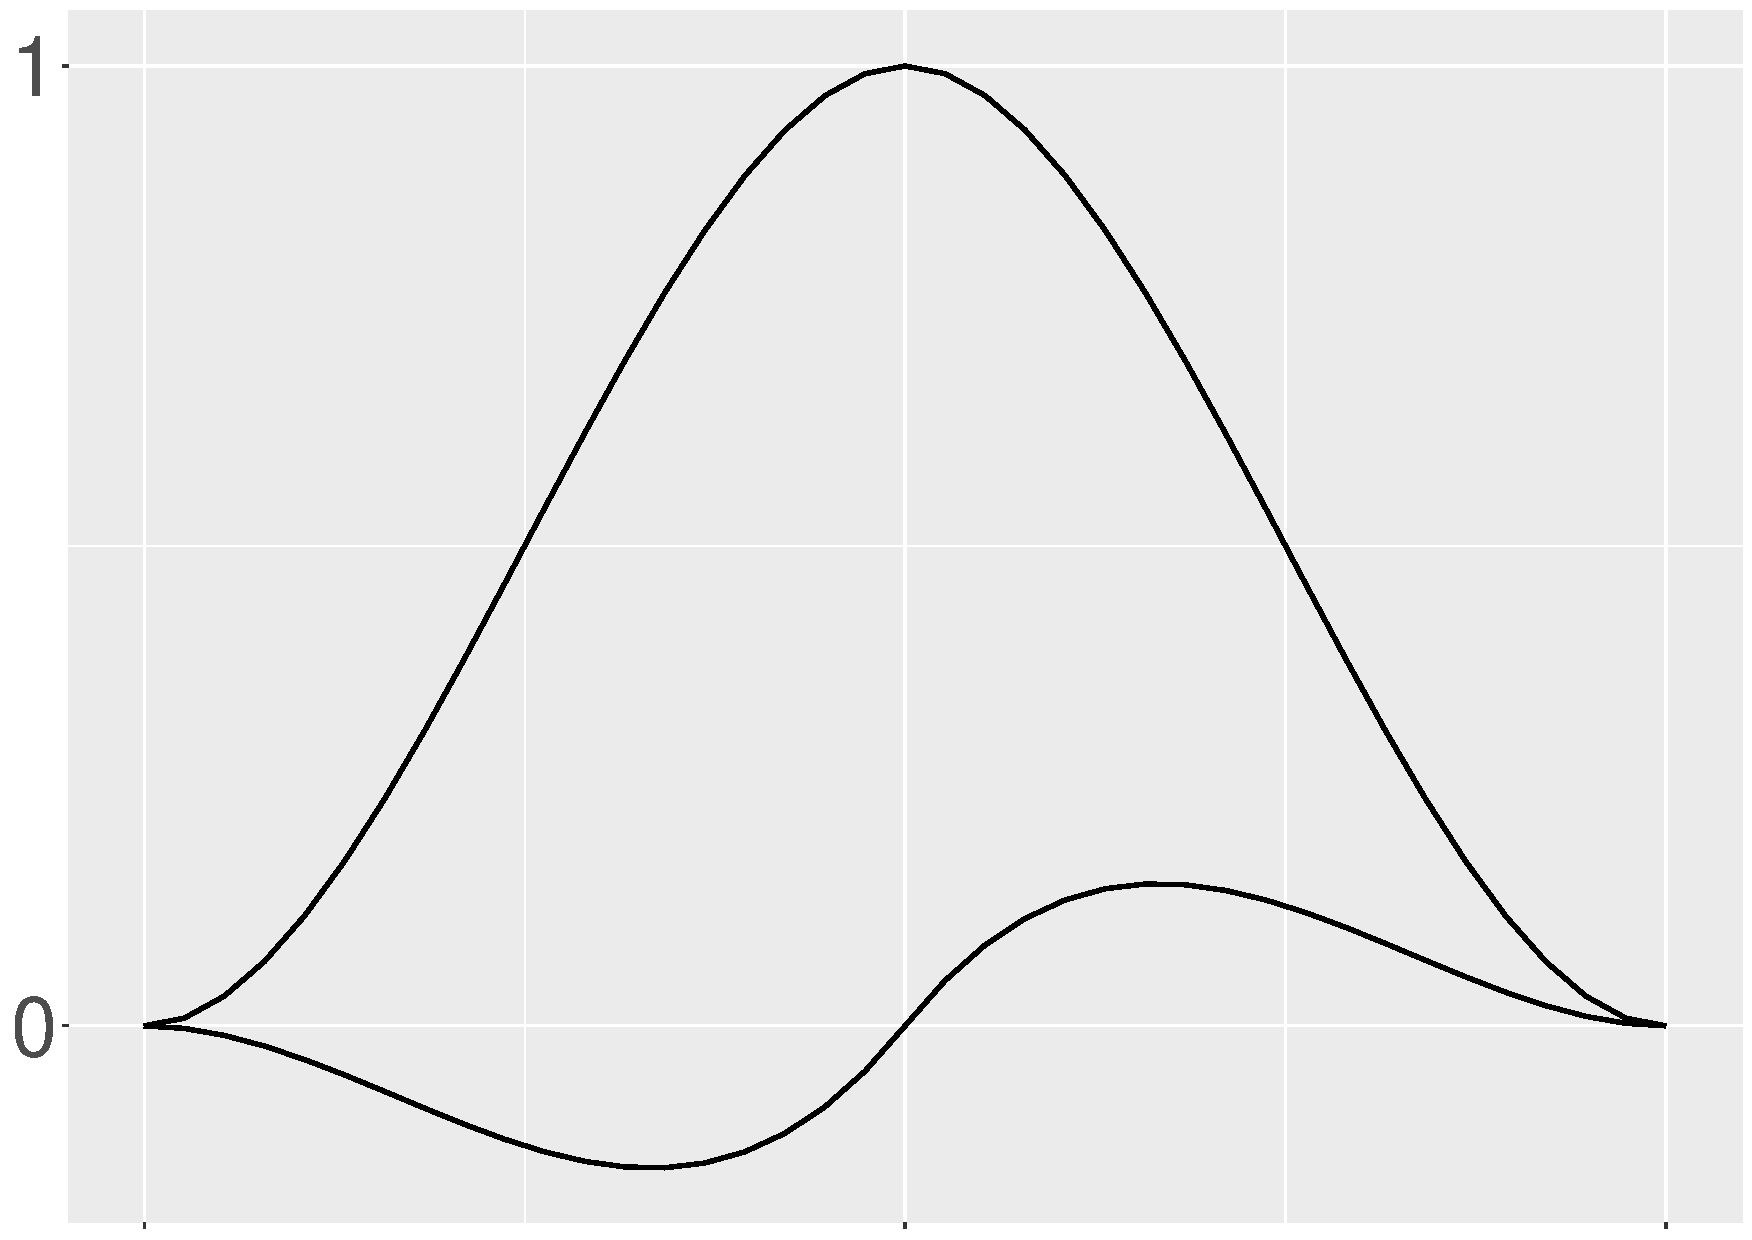
\includegraphics[width=0.7\textwidth,height=5cm]{Chapters/02TractorSplineTheory/plot/ggbasis.pdf}};
    \begin{scope}[
        x={(image.south east)},
        y={(image.north west)}
    ]
    \node [black, font=\bfseries] at (0.08,-0.02) {$t_i$};
    \node [black, font=\bfseries] at (0.52,-0.02) {$t_{i+1}$};
    \node [black, font=\bfseries] at (0.95,-0.02) {$t_{i+2}$};
    \end{scope}
\end{tikzpicture}
\caption{The two basis functions $N_{2i+1}$ (upper) and $N_{2i+2}$ (lower) on an arbitrary interval $[t_i, t_{i+2})$. Apparently, the basis functions are continuous on the interval and have continuous first derivatives.}\label{basisfigure}
\end{figure}

From the definition of basis functions, it can be seen that at the same knot of two neighbor intervals, Hermite spline basis functions share the same $y_i$ and $v_i$. With this property, we construct V-spline basis functions. 

Further, there are two parameters at each knot, hence the number of the degrees of freedom for parameters is $2n$.
%There are two parameters at each knot and four at the starting and ending knots. Hence, the number of the degrees of freedom for parameters is $2(n-2)+4=2n$.
However $2(n-2)$ constraints are added to the interior knots, at which the spline have continuous first and second derivatives. Additional two constraints are added to the starting and ending knots to keep their first derivatives continuous. Consequently, the number of the degrees of freedom for V-spline is 2. 


\subsection{Solution to The Objective Function}

Basis functions have been defined in the previous subsection, therefore the V-spline $f(t)$ on $[a,b]$, where $a \leq t_1 < t_2< \cdots < t_{n-1}<t_n \leq b$, can be found by minimizing  objective function \eqref{tractorsplineObjective}, which reduces to
\begin{equation}\label{tractormse}
\text{MSE}(\theta, \lambda,\gamma) = \left(\mathbf{y}-\mathbf{B}\theta\right)^\top \left(\mathbf{y}-\mathbf{B}\theta\right) +\gamma \left(\mathbf{v}-\mathbf{C}\theta\right)^\top \left(\mathbf{v}-\mathbf{C}\theta\right)+n \theta^\top\mathbf{\Omega}_{\lambda}\theta,
\end{equation}
where $\left\lbrace \mathbf{B}\right\rbrace_{ij} = N_j(t_i)$ , $\left\lbrace \mathbf{C}\right\rbrace_{ij} = N'_j(t_i)$ and $\left\lbrace \Omega_{2n}^{(i)} \right\rbrace_{jk}=\int_{t_i}^{t_{i+1}}\lambda_i N''_j(t)N''_k(t)dt$. After substituting the series observation $t_1, \ldots, t_n$ into basis functions, we get $N_1(t_1)=1, N_1(t_2)=0, \ldots, N_{2i-1}(t_{i})=1, N_{2i}(t_{i})=0, \ldots, N_{2n-1}(t_n)=1, N_{2n}(t_n)=0$; and into first derivative of basis functions, we get $N'_1(t_1)=0, N_1'(t_2)=1, \ldots, N_{2i-1}'(t_{i})=0, N_{2i}'(t_{i})=1, \ldots, N_{2n-1}'(t_n)=0, N_{2n}'(t_n)=1$. That means the matrices $\mathbf{B}$ and $\mathbf{C}$ in MSE equation \eqref{tractormse} are $n \times 2n$ dimensional and the elements are
\begin{align}
\mathbf{B}&=\left\lbrace B\right\rbrace_{ij}=\begin{cases}
1, & j=2i-1\\
0, & \mbox{otherwise}
\end{cases}\\
\mathbf{C}&=\left\lbrace C\right\rbrace_{ij}=\begin{cases}
1, & j=2i\\
0, & \mbox{otherwise}
\end{cases}
\end{align}
where $i=1, \ldots, n$, $j=1,\ldots,2n$ and $k=1,\ldots,2n$. The $i$-th $\Omega^{(i)}$ on the interval $[t_i,t_{i+1}]$ is a $2n \times 2n$ matrix and $\Omega^{(n)}$ does not exist. Its detail is in Appendix \ref{PenaltyTermDetails}. As a result, the penalty term is a bandwidth four matrix written in such a way:
\begin{equation}
\mathbf{\Omega}_\lambda=\sum_{i=1}^{n-1}\lambda_i\Omega^{(i)}.
\end{equation}



The solution to the equation \eqref{tractormse} is 
\begin{equation}\label{thetahat}
\hat{\theta}=\left(\mathbf{B}^\top\mathbf{B}+\gamma\mathbf{C}^\top\mathbf{C}+n\mathbf{\Omega}_{\lambda}\right)^{-1}\left(\mathbf{B}^\top\mathbf{y}+\gamma\mathbf{C}^\top\mathbf{v}\right)
\end{equation}
a generalized ridge regression. As a result, the fitted smoothing spline is given by
\begin{equation}
\hat{f}(t)=\sum_{k=1}^{2n}N_k(t)\hat{\theta}_k
\end{equation}

A smoothing spline with parameters $\lambda(t)$ and $\gamma$ is an example of a linear smoother \citep{esl2009}. This is because the estimated parameters in equation \eqref{thetahat} are a linear combination of $y_i$ and $v_i$. Denote by $\hat{\mathbf{f}}$ and $\hat{\mathbf{f}'}$ the $2n$ vector of fitted values $\hat{f}(t_i)$ and $\hat{f'}(t_i)$ at the training points $t_i$. Then
\begin{equation}
\begin{split}
\hat{\mathbf{f}} =&\mathbf{B}\left(\mathbf{B}^\top\mathbf{B}+\gamma\mathbf{C}^\top\mathbf{C}+n\mathbf{\Omega}_{\lambda}\right)^{-1}\left(\mathbf{B}^\top\mathbf{y}+\gamma\mathbf{C}^\top\mathbf{v}\right)\\
\triangleq & \mathbf{S}_{\lambda,\gamma}\mathbf{y}+\gamma\mathbf{T}_{\lambda,\gamma}\mathbf{v} 
\end{split}
\end{equation}
\begin{equation}
\begin{split}
\hat{\mathbf{f}'}
=&\mathbf{C}\left(\mathbf{B}^\top\mathbf{B}+\gamma\mathbf{C}^\top\mathbf{C}+n\mathbf{\Omega}_{\lambda}\right)^{-1}\left(\mathbf{B}^\top\mathbf{y}+\gamma\mathbf{C}^\top\mathbf{v}\right)\\
\triangleq&\mathbf{U}_{\lambda,\gamma}\mathbf{y}+\gamma\mathbf{V}_{\lambda,\gamma}\mathbf{v}
\end{split}
\end{equation}
The fitted $\hat{\mathbf{f}}$ and $\hat{\mathbf{f}'}$ are linear in $\mathbf{y}$ and $\mathbf{v}$, and the finite linear operators $\mathbf{S}_{\lambda,\gamma}, \mathbf{T}_{\lambda,\gamma}, \mathbf{U}_{\lambda,\gamma}$ and $\mathbf{V}_{\lambda,\gamma}$ are known as the smoother matrices. One consequence of this linearity is that the recipe for producing $\hat{\mathbf{f}}$ and $\hat{\mathbf{f}'}$ from $\mathbf{y}$ and $\mathbf{v}$, do not depend on $\mathbf{y}$ and $\mathbf{v}$ themselves; $\mathbf{S}_{\lambda,\gamma}, \mathbf{T}_{\lambda,\gamma}, \mathbf{U}_{\lambda,\gamma}$ and $\mathbf{V}_{\lambda,\gamma}$ depend only on $t_i,\lambda(t)$ and $\gamma$.

Suppose in a traditional least squares fitting, $\mathbf{B}_\xi$ is $N \times M$ matrix of $M$ cubic-spline basis functions evaluated at the $N$ training points $x_i$, with knot sequence $\xi$ and $M \ll N$. Thus the vector of fitted spline values is given by
\begin{align}\label{fhy}
\hat{\mathbf{f}}=\mathbf{B}_\xi\left(\mathbf{B}^\top_\xi\mathbf{B}_\xi\right)^{-1}\mathbf{B}_\xi\mathbf{y}=\mathbf{H}_\xi\mathbf{y}
\end{align}
Here the linear operator $\mathbf{H}_\xi$ is a symmetric, positive semidefinite matrices, and $\mathbf{H}_\xi\mathbf{H}_\xi=\mathbf{H}_\xi$ (idempotent) \citep{esl2009}. In our case, it is easily seen that $\mathbf{S}_{\lambda,\gamma}, \mathbf{T}_{\lambda,\gamma}, \mathbf{U}_{\lambda,\gamma}$ and $\mathbf{V}_{\lambda,\gamma}$ are symmetric, positive semidefinite matrices as well. Additionally, by Cholesky decomposition
\begin{equation}
\left(\mathbf{B}^\top\mathbf{B}+\gamma\mathbf{C}^\top\mathbf{C}+n\mathbf{\Omega}_{\lambda}\right)^{-1}=\mathbf{R}\mathbf{R}^\top,
\end{equation}
it is easy to prove that $\mathbf{T}_{\lambda,\gamma}=\mathbf{B}\mathbf{R}\mathbf{R}^\top\mathbf{C}^\top$ and $\mathbf{U}_{\lambda,\gamma}=\mathbf{C}\mathbf{R}\mathbf{R}^\top\mathbf{B}^\top$, then we will have 
 $\mathbf{T}_{\lambda,\gamma}= \mathbf{U}_{\lambda,\gamma}^\top$. When $\lambda=\gamma=0$, the matrix $\mathbf{S}_{\lambda_0,\gamma_0}=\mathbf{B}\left(\mathbf{B}^\top\mathbf{B}\right)^{-1}\mathbf{B}^\top$ is idempotent.  


\begin{corollary}\label{TractorsplineCorollary}
If $f(t)$ is the V-spline on the entire interval $[t_1,t_n]$, for sufficient cases of $\lambda(t)$ and $\gamma$, $f(t)$ has the following property:
\begin{enumerate}\itemsep0em 
\item if $\lambda(t)$ is piecewise constant and $\gamma \neq 0$, then $f$ and $f'$ are continuous, $f''$ is piecewise linear but not continuous at knots;
\item if $\lambda(t)$ is piecewise constant and $\gamma = 0$, the same as above;
\item if $\lambda(t)=\lambda $ is constant on the entire interval and $\gamma \neq 0$, the same as above;
\item if $\lambda(t)=\lambda $ is constant on the entire interval and $\gamma = 0$, then $f$, $f'$ are continuous, $f''$ is piecewise linear and continuous at knots.
\end{enumerate}
\end{corollary}

The proof of Corollary \ref{TractorsplineCorollary} is in Appendix \ref{proofofCorollary}. 

%Then we take some sample knots $\mathbf{y}^{(new)}$ with the same size of $\mathbf{y}$ from $\hat{\mathbf{f}}$ and reconstruct the spline function. It is easily seen that
% \begin{equation}
%\hat{\mathbf{f}}^{(new)} = \mathbf{S}_{\lambda_0,\gamma_0}\mathbf{y}^{(new)}=\mathbf{S}_{\lambda_0,\gamma_0}\mathbf{S}_{\lambda_0,\gamma_0}\mathbf{y}=(\mathbf{B}(\mathbf{B}^\top\mathbf{B})^{-1}\mathbf{B}^\top)(\mathbf{B}(\mathbf{B}^\top\mathbf{B})^{-1}\mathbf{B}^\top)=\mathbf{S}_{\lambda_0,\gamma_0}\mathbf{y},
 %\end{equation}
 %which returns the same reconstruction. So $\hat{\mathbf{f}}$ is generated and only affected by $\mathbf{y}$. And the same as $\hat{\mathbf{f}'}$, because
%\begin{equation}
%\hat{\mathbf{f}'}^{(new)}=\mathbf{U}_{\lambda_0,\gamma_0}\mathbf{y}^{(new)}=\mathbf{U}_{\lambda_0,\gamma_0}\mathbf{S}_{\lambda_0,\gamma_0}\mathbf{y}=(\mathbf{C}\mathbf{B} (\mathbf{B}^\top\mathbf{B})^{-1}\mathbf{B}^\top)(\mathbf{B}(\mathbf{B}^\top\mathbf{B})^{-1}\mathbf{B}^\top)\mathbf{y}=\mathbf{U}_{\lambda_0,\gamma_0}\mathbf{y}.
%\end{equation}
 %That means no matter how many times we reconstruct V-spline, once the matrices are fixed and observed knots are given, it will always return the same results when $\lambda=\gamma=0$.

%\begin{theorem}
%For $n\geq 2$, the objective function $J[f]$ in equation \eqref{tractorsplineObjective} is minimized by a V-spline.
%\end{theorem}



\subsection{Adjusted Penalty Term and Parameter Function}

To get the reconstructed trajectory in a multi-dimensional space, one can use the V-spline to find the trajectory in each dimension separately and then combine them together for a higher dimension, such as 2D and 3D. Typically, the data are not regularly sampled in time. Due to the property of Hermite spline, the combination of a multi-dimensional reconstruction for irregular time difference dataset will bring some issues.  Image the situation that a vehicle is moving along the $x$-axis, but stays unchanged on its $y$ position. By fitting $\mathbf{x}$ and $\mathbf{u}$, the V-spline $f_x(t)$ will give us the best fit which returns smallest errors to the objective function. While with the same parameter $\lambda(t)$ and $\gamma$, $f_y(t)$ returns a cubic curve, where it should give us a straight line as we expected. Moreover, in some circumstances, with time increasing $\mathbf{f}$ and $\mathbf{f}'$ remain the same, or change slightly. In this situation, the Hermite spline will return wiggles in each dimension and curves in combined two dimensions. 

To get a reliable reconstruction, we introduce an adjusted penalty term $\frac{\left(\Delta t_i\right)^\alpha}{\left(\Delta d_i\right)^\beta}$, where $\alpha \ge 0$ and $\beta \ge 0$, to the penalty function $\lambda(t)$, in which the V-spline is penalized by its real difference of $\Delta d_i$ and $\Delta t_i$ for each interval $[t_i, t_{i+1}]$. With this term, when either $\mathbf{u}$ for $x$ or $\mathbf{v}$ for $y$ goes down or equals to 0, it will make sure that the penalty function will be large enough and returns a straight line rather than a curve on this domain. Because of the unit of the penalty term is $m^2/t^3$, to keep the same scale, $\alpha$ and $\beta$ in the adjusted penalty term are chosen as $3$ and $2$ respectively. From the physical point of view, the term is the reciprocal of the product of velocity and acceleration. Either velocity or acceleration goes to zero, the moving object should either stop, which returns a straight line through time on $x$ or $y$ axes and a dot on the higher dimension or keep moving with the same speed, which returns a linear instead of a curved path. 

Thus, the final form of the penalty function is 
\begin{equation}\label{adjustedpenalty}
\lambda(t)=\frac{\left(\Delta t_i\right)^3}{\left(\Delta d_i\right)^2}\lambda,
\end{equation}
where  $t_i\leq t < t_{i+1}$. Eventually, in the objective function, there is one parameter $\lambda$ controlling the curvature of V-spline on different domains, and another one $\gamma$ controlling the residuals of velocity. 




\section{Parameter Selection and Cross-Validation}

The problem of choosing the smoothing parameter is ubiquitous in curve estimation, and there are two different philosophical approaches to this question. The first one is to regard the free choice of smoothing parameter as an advantageous feature of the procedure. The other one is to find the parameter automatically by the data \citep{green1993nonparametric}. We prefer the latter one, use data to train our model and find the best parameters. The most well-known method is cross-validation.


Assuming that mean of the random errors is zero, the true regression curve $f(t)$ has the property that, if an observation $y$ is taken away at a point $t$, the value $f(t)$ is the best predictor of $y$ in terms of returning a least value of $\left(y-f(t)\right)^2$. 

Now, focus on an observation $y_i$ at point $t_i$ as being a new observation by omitting it from the set of data, which are used to estimate $\hat{f}$. Denote by $\hat{f}^{(-i)}(t,\lambda)$ the estimated function from the remaining data, where $\lambda$ is the smoothing parameter. Then $\hat{f}^{(-i)}\left(t,\lambda\right)$ is the minimizer of  
\begin{equation}\label{originalcv}
\frac{1}{n}\sum_{j \neq i}\left(y_j-f(t_j) \right)^2+\lambda\int (f'')^2dt,
\end{equation}
and can be quantified by the cross-validation score function
\begin{equation*}
\mbox{CV}(\lambda)=\frac{1}{n}\sum_{i=1}^{n}\left(  y_i-\hat{f}^{(-i)}(t_i,\lambda)\right) ^2.
\end{equation*}
The basis idea of the cross-validation is to choose the value of $\lambda$ that minimizes $\mbox{CV}(\lambda)$ \citep{green1993nonparametric}. 

%An efficient way to calculate the cross-validation score is introduced by \citep{green1993nonparametric}. 
Through the equation \eqref{fhy}, it is known that the value of the smoothing spline $\hat{f}$ depend linearly on the data $y_i$. Define the matrix $A(\lambda)$, which is a map vector of observed values $y_i$ to predicted values $\hat{f}(t_i)$. Then we have
\begin{equation*}\label{crossvalidationmatrixA}
\hat{\mathbf{f}}=A(\lambda)\mathbf{y}
\end{equation*}
and the following lemma.
\begin{lemma}\label{cvlema}
The cross-validation score satisfies
\begin{equation*}
\mbox{CV}(\lambda)=\frac{1}{n} \sum_{i=1}^n \left(\frac{y_i-\hat{f}(t_i)}{1-A_{ii}(\lambda)}\right)^2
\end{equation*}
where $\hat{f}$ is the spline smoother calculated from the full data set $\left\lbrace (t_i,y_i)\right\rbrace$ with smoothing parameter $\lambda$.
\end{lemma}

For a V-spline and its MSE function, there are two parameters $\lambda(t)$ and $\gamma$ to be estimated for. Therefore, $\hat{f}^{(-i)}(t,\lambda)$ is the minimizer of  
\begin{align}
\frac{1}{n}\sum_{j \neq i}\left( y_j-f(t_j) \right)^2+\frac{\gamma}{n}\sum_{j \neq i} \left( v_j-f'(t_j) \right)^2+ \int \lambda(t) \left( f'' \right)^2dt,
\end{align}
and the cross-validation score function is
\begin{align}
\mbox{CV}\left(\lambda(t),\gamma\right)=\frac{1}{n}\sum_{i=1}^{n}\left( y_i-\hat{f}^{(-i)}\left(t_i,\lambda(t),\gamma\right) \right) ^2.
\end{align}
Additionally, it is known that the parameter $\hat{\theta}=\left(B^\top B+\gamma C^\top C+n\Omega_\lambda\right)^{-1}\left(B^\top\mathbf{y}+\gamma C^\top\mathbf{v}\right)$ and will give us the following form \small
\begin{equation}
\begin{split}
 \hat{\mathbf{f}}&=B\hat{\theta}=B\left(B^\top B+\gamma C^\top C+n\Omega_\lambda\right)^{-1}B^\top\mathbf{y}+B\left(B^\top B+\gamma C^\top C+n\Omega_\lambda\right)^{-1} C^\top\mathbf{v}\\&=S\mathbf{y}+\gamma T\mathbf{v},
 \end{split}
 \end{equation}
 \begin{equation}
 \begin{split}
\hat{\mathbf{f}}'&=C\hat{\theta}=C\left(B^\top B+\gamma C^\top C+n\Omega_\lambda\right)^{-1}B^\top\mathbf{y}+C\left(B^\top B+\gamma C^\top C+n\Omega_\lambda\right)^{-1}C^\top \mathbf{v}\\&=U\mathbf{y}+\gamma V\mathbf{v}.
 \end{split}
\end{equation}\normalsize
From Lemma \ref{cvlema}, we can prove the following theorem: 
\begin{theorem}\label{tractorsplinecvscore}
The cross-validation score of a V-spline satisfies
\begin{equation}\label{tractorcv}
\mbox{CV}\left(\lambda(t),\gamma\right)=\frac{1}{n}\sum_{i=1}^{n} \left( \frac{\hat{f}(t_i)-y_i+\gamma \frac{T_{ii}}{1-\gamma V_{ii}}(\hat{f}'(t_i)-v_i)}{1-S_{ii}-\gamma\frac{T_{ii}}{1-\gamma V_{ii}}U_{ii}} \right)^2
\end{equation}
where $\hat{f}$ is the V-spline smoother calculated from the full data set $\left\lbrace (t_i,y_i,v_i)\right\rbrace$ with smoothing parameter $\lambda(t)$ and $\gamma$.
\end{theorem}

The proof of Theorem \ref{tractorsplinecvscore} follows immediately from a lemma, and gives an expression for the deleted residuals $y_i-\hat{f}^{(-i)}(t_i)$ and $v_i-\hat{f}'^{(-i)}(t_i)$ in terms of $y_i-\hat{f}(t_i)$ and $v_i-\hat{f}'(t_i)$ respectively. 

\begin{lemma} \label{cvlemma}
For fixed $\lambda(t),\gamma$ and $i$, denote $\mathbf{f}^{(-i)}$ by the vector with components $f_j^{(-i)}=\hat{f}^{(-i)}\left(t_j,\lambda(t),\gamma\right)$,  $\mathbf{f}'^{(-i)}$ by the vector with components $f_j'^{(-i)}=\hat{f}'^{(-i)}\left(t_j,\lambda(t),\gamma\right)$, and define vectors $\mathbf{y}^*$ and $\mathbf{v}^*$ by 
\begin{align}
\begin{cases}
y_j^*=y_j &j \neq i\\
y_i^*=\hat{f}^{(-i)}(t_i) &\mbox{otherwise}
\end{cases}\\
\begin{cases}
v_j^*=v_j &j \neq i\\
v_i^*=\hat{f}'^{(-i)}(t_i) &\mbox{otherwise}
\end{cases}
\end{align}
Then
\begin{align}
\mathbf{\hat{f}}^{(-i)}&=S\mathbf{y}^*+\gamma T\mathbf{v}^*\\
\mathbf{\hat{f}}'^{(-i)}&=U\mathbf{y}^*+\gamma V\mathbf{v}^*
\end{align}
\end{lemma}


\section{Simulation Study} %and Error Analysis}


\subsection{Numerical Examples}

In this section, we examine the visual quality of the proposed method with four functions: \textit{Blocks}, \textit{Bumps}, \textit{HeaviSine} and \textit{Doppler}, which have been used in \citep{donoho1994ideal, donoho1995adapting, abramovich1998wavelet} because of their caricature features in imaging, spectroscopy and other scientific signal processing. However it is unfair for V-spline fitting "jump" position in \textit{Blocks} and \textit{Bumps} function because it fits position and velocity simultaneously and these points imply infinite first derivative in original functions, which are impossible for vehicles or individuals. In terms of this issue, we treat these functions as velocity, and use noise free points to generate accurate position data, then add noises back to them.

For calculating consideration, we use $n=1024$ \citep{nason2010wavelet}. Because of all noises are randomly generated, for the convenience of reinitialization and repeatable comparison, we set random seed at 2016. The noises are \iid zero-mean Gaussian distributed with standard deviation regarding to signal-to-noise ratio (SNR), which specifies the ratio of the standard deviation of the function to the standard deviation of the simulated errors. Explicitly, if the standard deviation of the true signal $f$ is $\sigma_f$, the simulated data will be $f+\varepsilon$, where the simulated error  $\varepsilon \sim N(0,\sigma_f/SNR)$. 

If the original function $g(t)$ is treated as velocity function $f'(t)=g(t)$, thus by setting initial position $y_0=0$, acceleration $a_0=0$ and using the following formula 
\begin{equation}\label{generateVelocity}
f(t_{i+1})=f(t_i)+\left(g(t_i)+g(t_{i+1}) \right)\frac{t_{i+1}-t_i}{2}
\end{equation}
for calculating position information, we can generate simulated data. Further, we add some \iid  zero-mean $\varepsilon$ noises with SNR to them to get the measurements by 
\begin{align}\label{tractorsplinegeneratefunctions}
\begin{split}
y_i &= f(t_i) + \varepsilon_f, \\
v_i &= g(t_i) + \varepsilon_g,
\end{split}
\end{align}
where $\varepsilon_f\sim N(0,\sigma_f/SNR)$ and $\varepsilon_g\sim N(0,\sigma_g/SNR)$. The value of SNR can be chosen 7 or 3. For wavelet transform reconstructions, we use the threshold policy of \textit{sure} and \textit{BayesThresh} with levels $l=4, \ldots, 9$ \citep{donoho1995adapting, abramovich1998wavelet}. A semi-parametric regression model with spatially adaptive penalized splines (\textit{P-spline}) is added in comparison  \citep{krivobokova2008fast, ruppert2003semiparametric}.

For V-spline, we have two parameters $\lambda$ and $\gamma$ to optimize. To evaluate the performance of the velocity term in objective function \eqref{tractorsplineObjective} and the adjusted penalty term in \eqref{adjustedpenalty}, the parameter $\gamma$ is set as 0 in one reconstruction of V-spline, whose objective function and solution become
\begin{equation}\label{ofgamma0}
J[f]_{\gamma=0}= \frac{1}{n} \sum_{i=1}^{n} \left(f(t_i)-y_i\right)^2 +\sum_{i=1}^{n-1} \lambda_i\int_{t_i}^{t_{i+1}} \left(f''\right)^2 dt,
\end{equation}
and
\begin{equation}\label{thetahat0}
\hat{\theta}_{\gamma=0}=\left(\mathbf{B}^\top\mathbf{B}+n\Omega_{\lambda}\right)^{-1}\mathbf{B}^\top\mathbf{y}
\end{equation}
and the adjusted penalty term in \eqref{adjustedpenalty} was removed from another reconstruction, noted as "V-spline without APT". Figure \ref{num1} to \ref{num4} display the original (velocity), generated position, wavelet with two different threshold methods, P-spline and three kinds of V-spline fitted functions. The parameters $\lambda$ and $\gamma$ of a V-spline are automatically selected with the formula \eqref{tractorcv} by $\textsf{optim}$ function in $R$ \citep{nelder1965simplex}.


%\begin{figure}
%  \centering
%   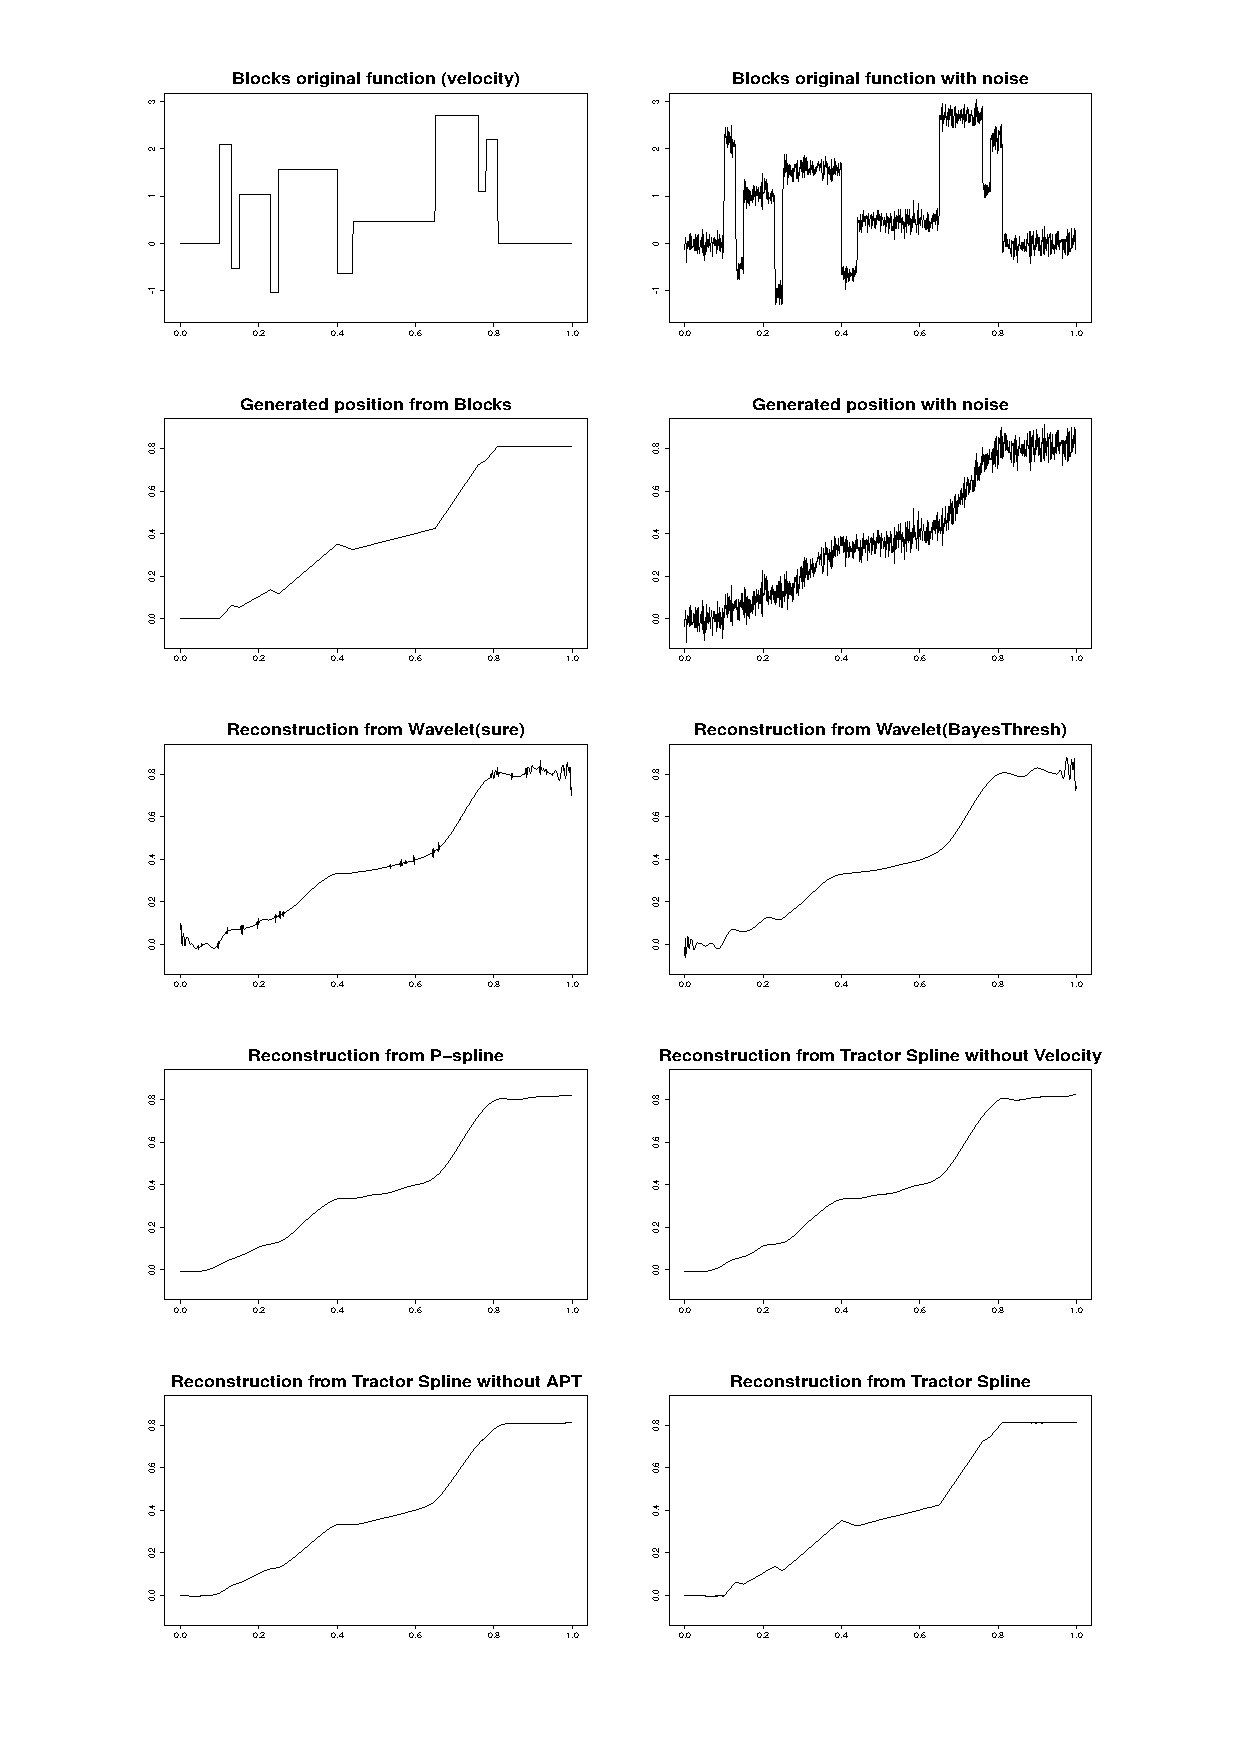
\includegraphics[width=\textwidth,height=14cm]{Chapters/02TractorSplineTheory/plot/blocks10} 
%  \caption{Numerical example: $\textit{Blocks}$. (a) The true velocity function. (b) Velocity with Gaussian noise at SNR=7. (c) Generated position function. (d) Position with Gaussian noise at SNR=7. (e) Reconstruction from Wavelet with sure threshold. (f) Reconstruction from Wavelet with BayesThresh approach. (g) Reconstruction by P-spline. (h) Reconstruction by V-spline setting $\gamma=0$. (i) Reconstruction by V-spline with normal penalty term. (j) Reconstruction by proposed V-spline.}\label{num1}
%\end{figure}

\begin{figure}
    \centering
    \begin{subfigure}{0.45\textwidth}
    \centering
    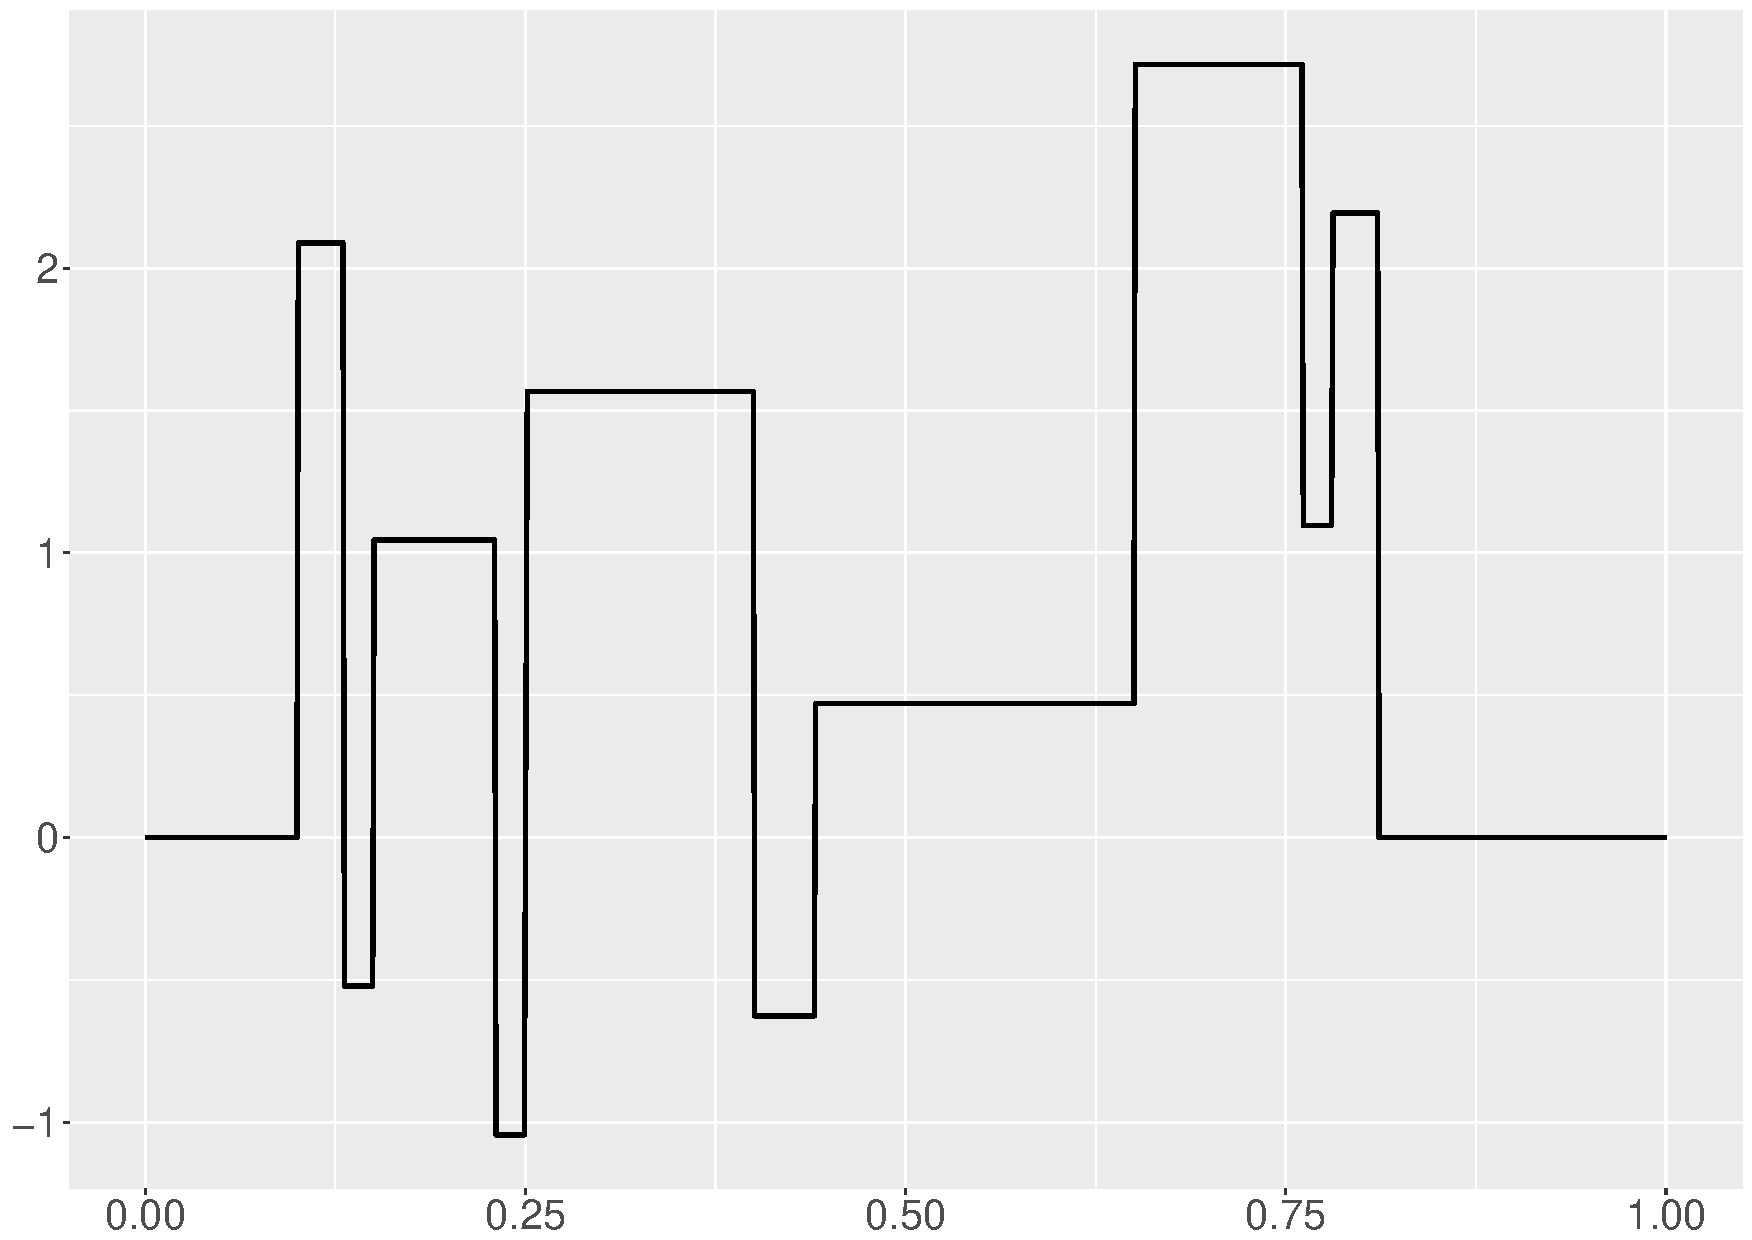
\includegraphics[width=\linewidth,height=0.45\textwidth]{Chapters/02TractorSplineTheory/plot/ggplot/ggBlocks.pdf}
    \caption{The \textit{Blocks} function}
    \end{subfigure}%
    \begin{subfigure}{0.45\textwidth}
    \centering
    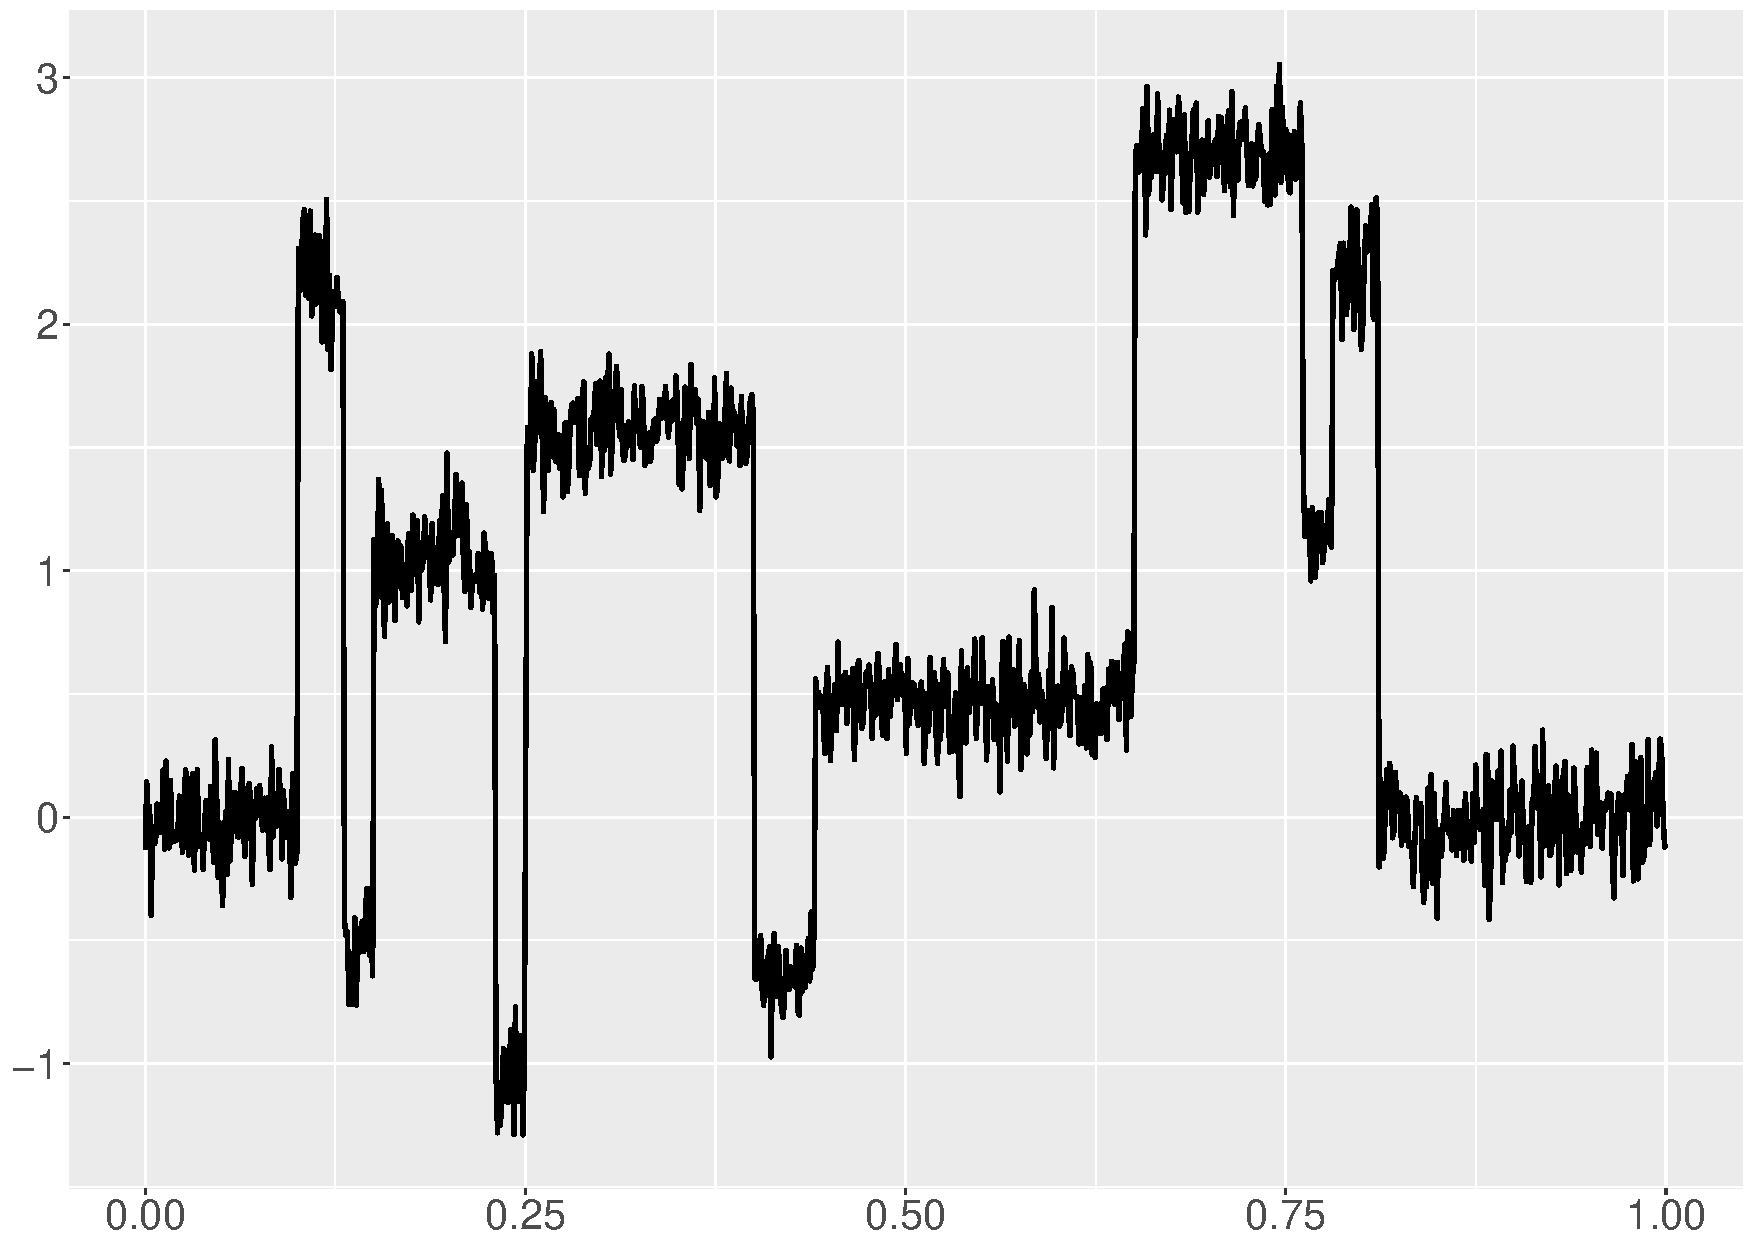
\includegraphics[width=\linewidth,,height=0.45\textwidth]{Chapters/02TractorSplineTheory/plot/ggplot/ggBlocksNoise.pdf}
    \caption{Noisy \textit{Blocks} at \textit{SNR}=7}
    \end{subfigure}
    \begin{subfigure}{0.45\textwidth}
    \centering
    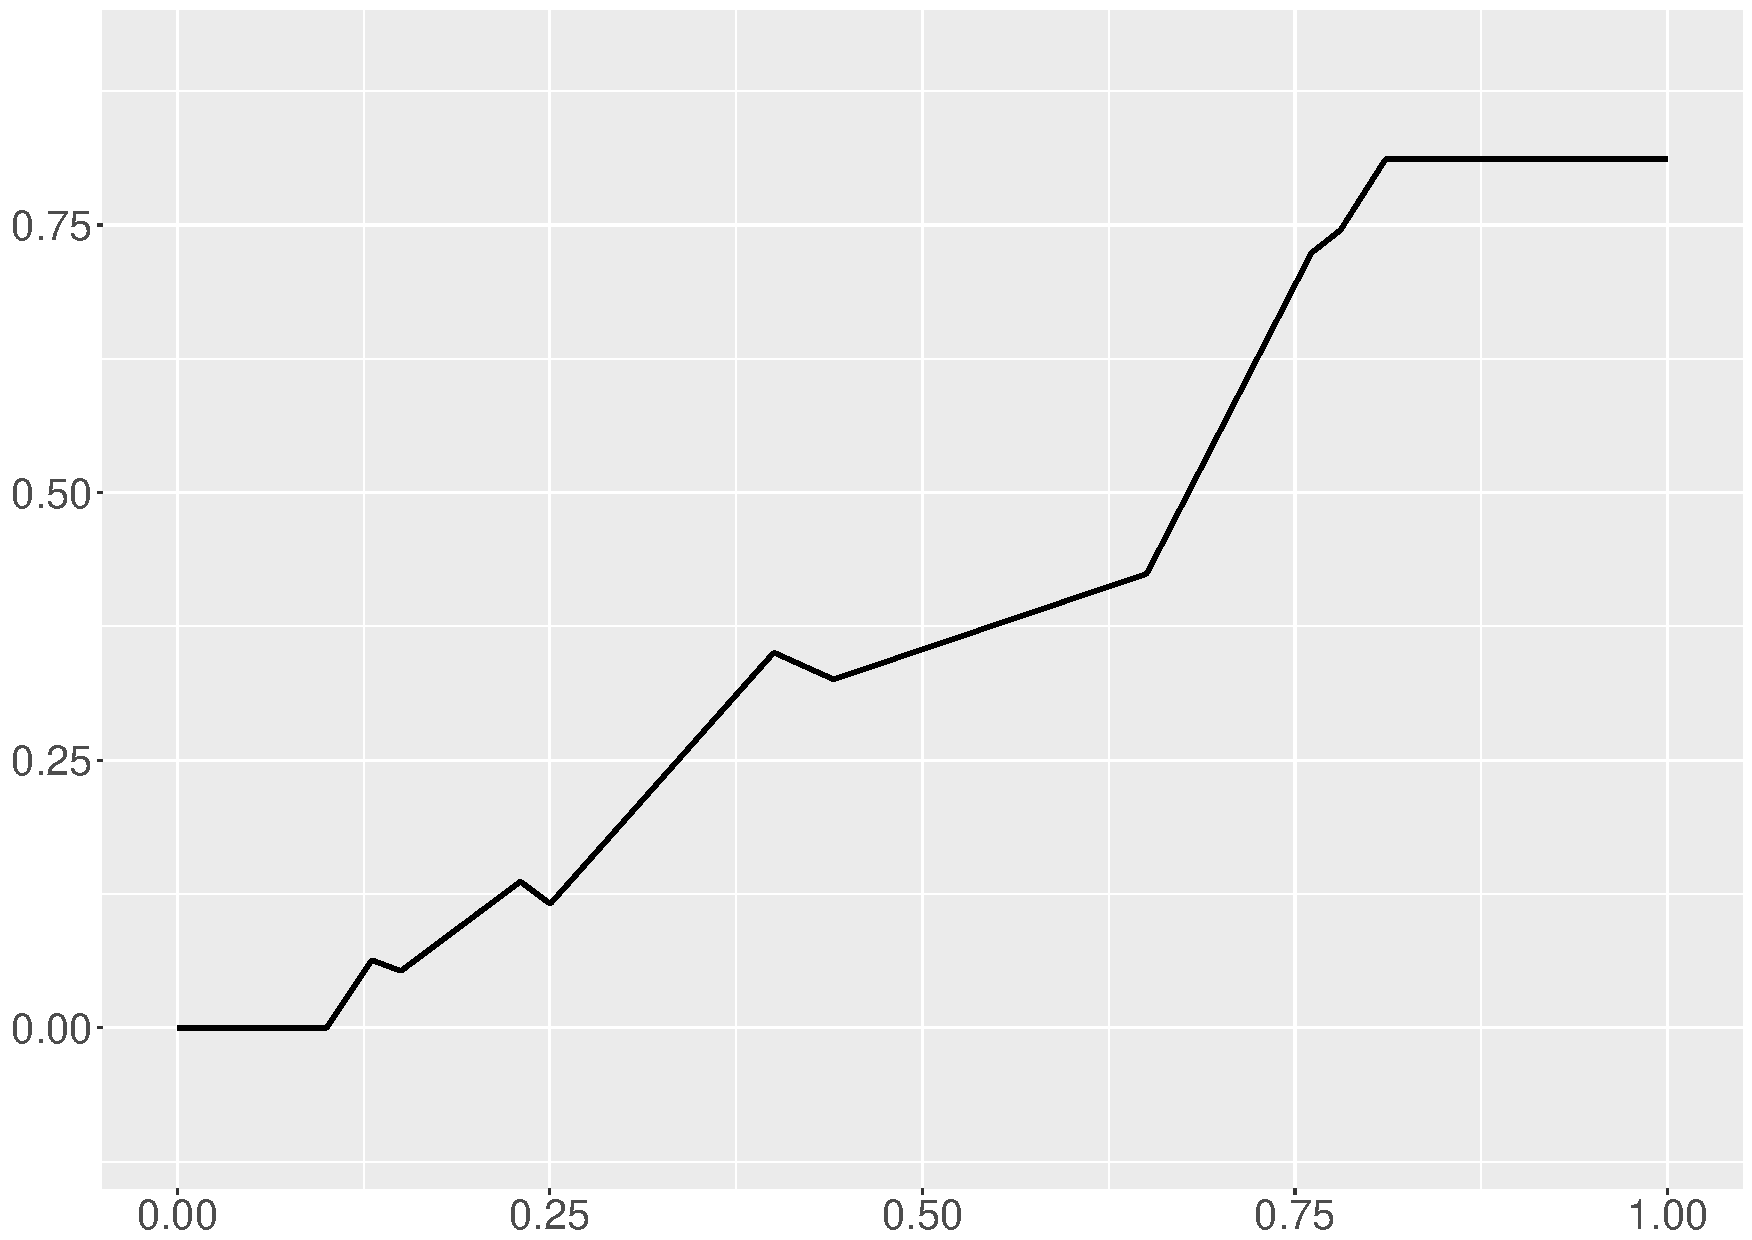
\includegraphics[width=\linewidth,height=0.45\textwidth]{Chapters/02TractorSplineTheory/plot/ggplot/ggBlocksPosition.pdf}
    \caption{Generated positions}
    \end{subfigure}
    \begin{subfigure}{0.45\textwidth}
    \centering
    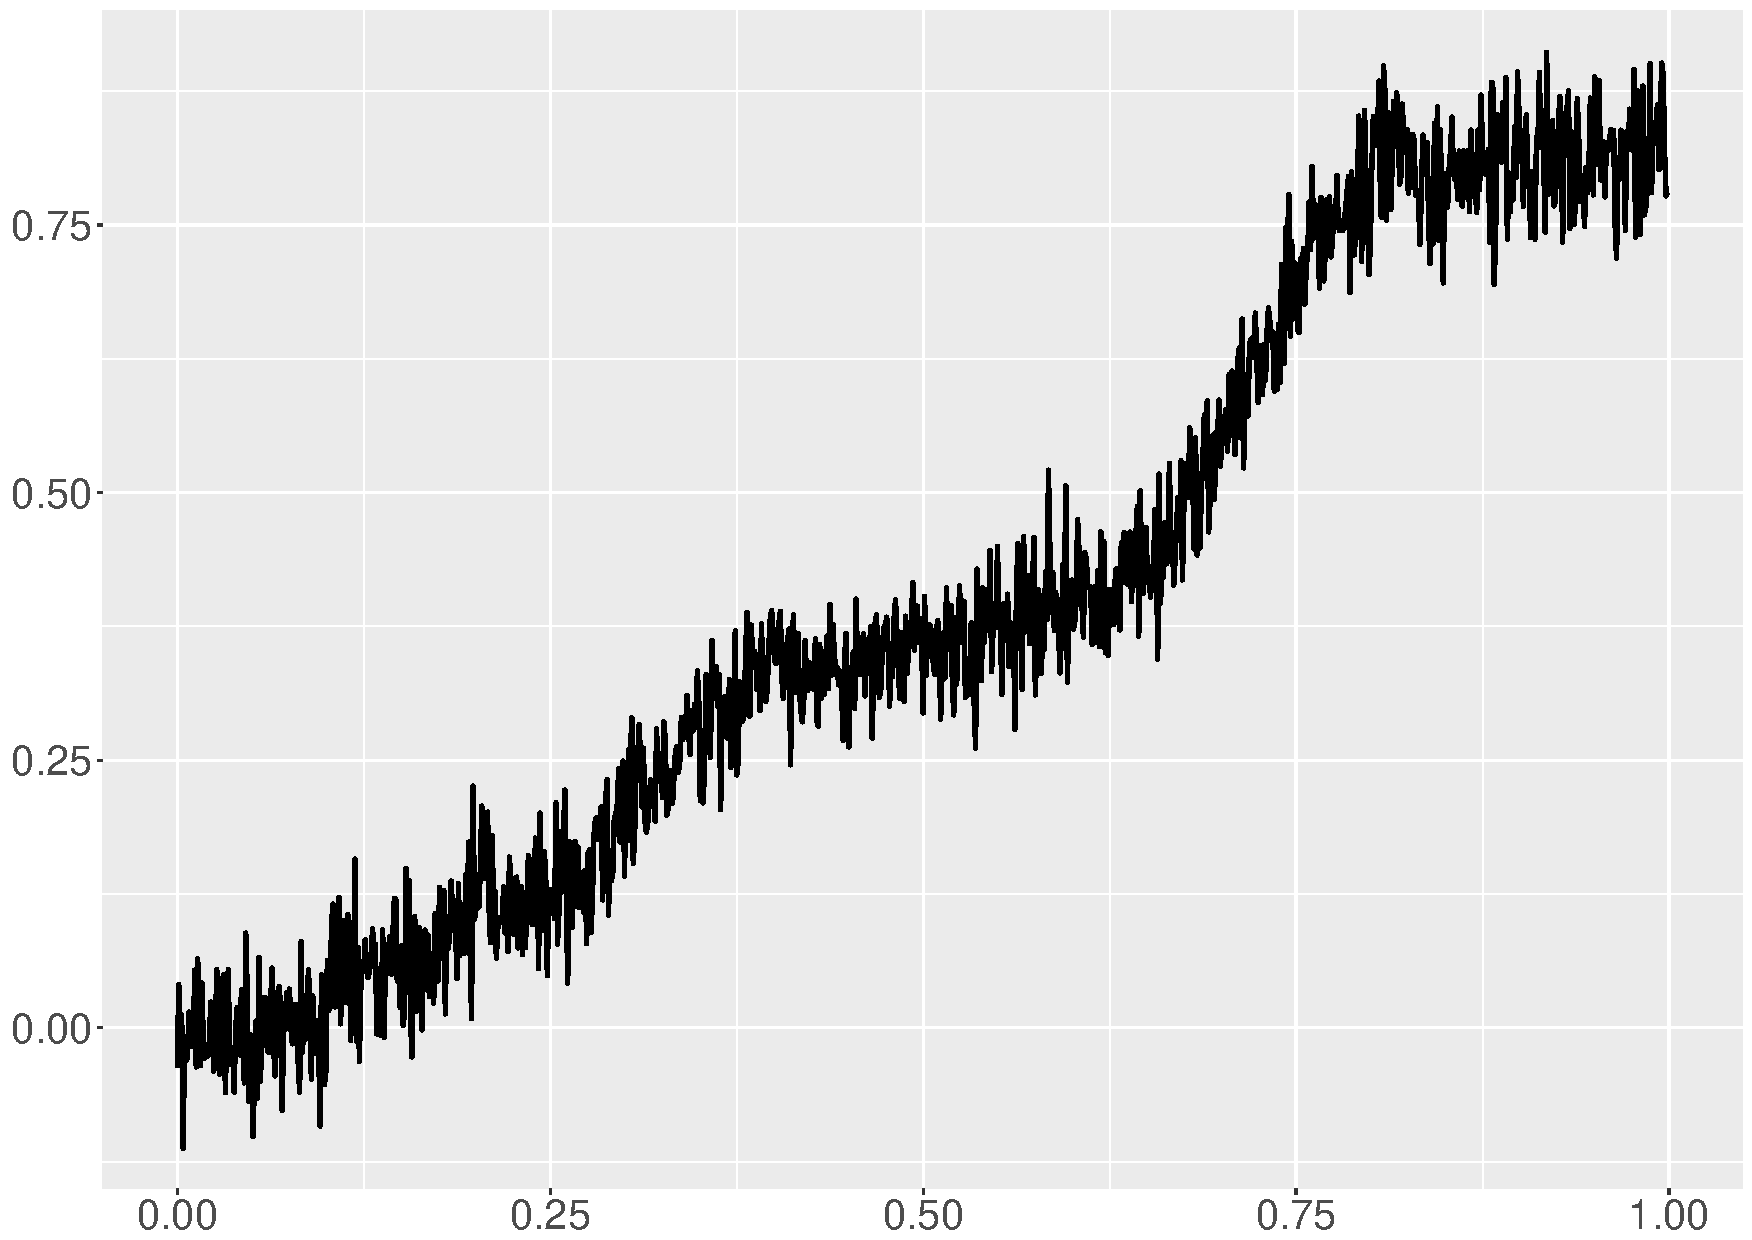
\includegraphics[width=\linewidth,height=0.45\textwidth]{Chapters/02TractorSplineTheory/plot/ggplot/ggBlocksPositionNoise.pdf}
    \caption{Noisy position at \textit{SNR}=7}
    \end{subfigure}
    \begin{subfigure}{0.45\textwidth}
    \centering
    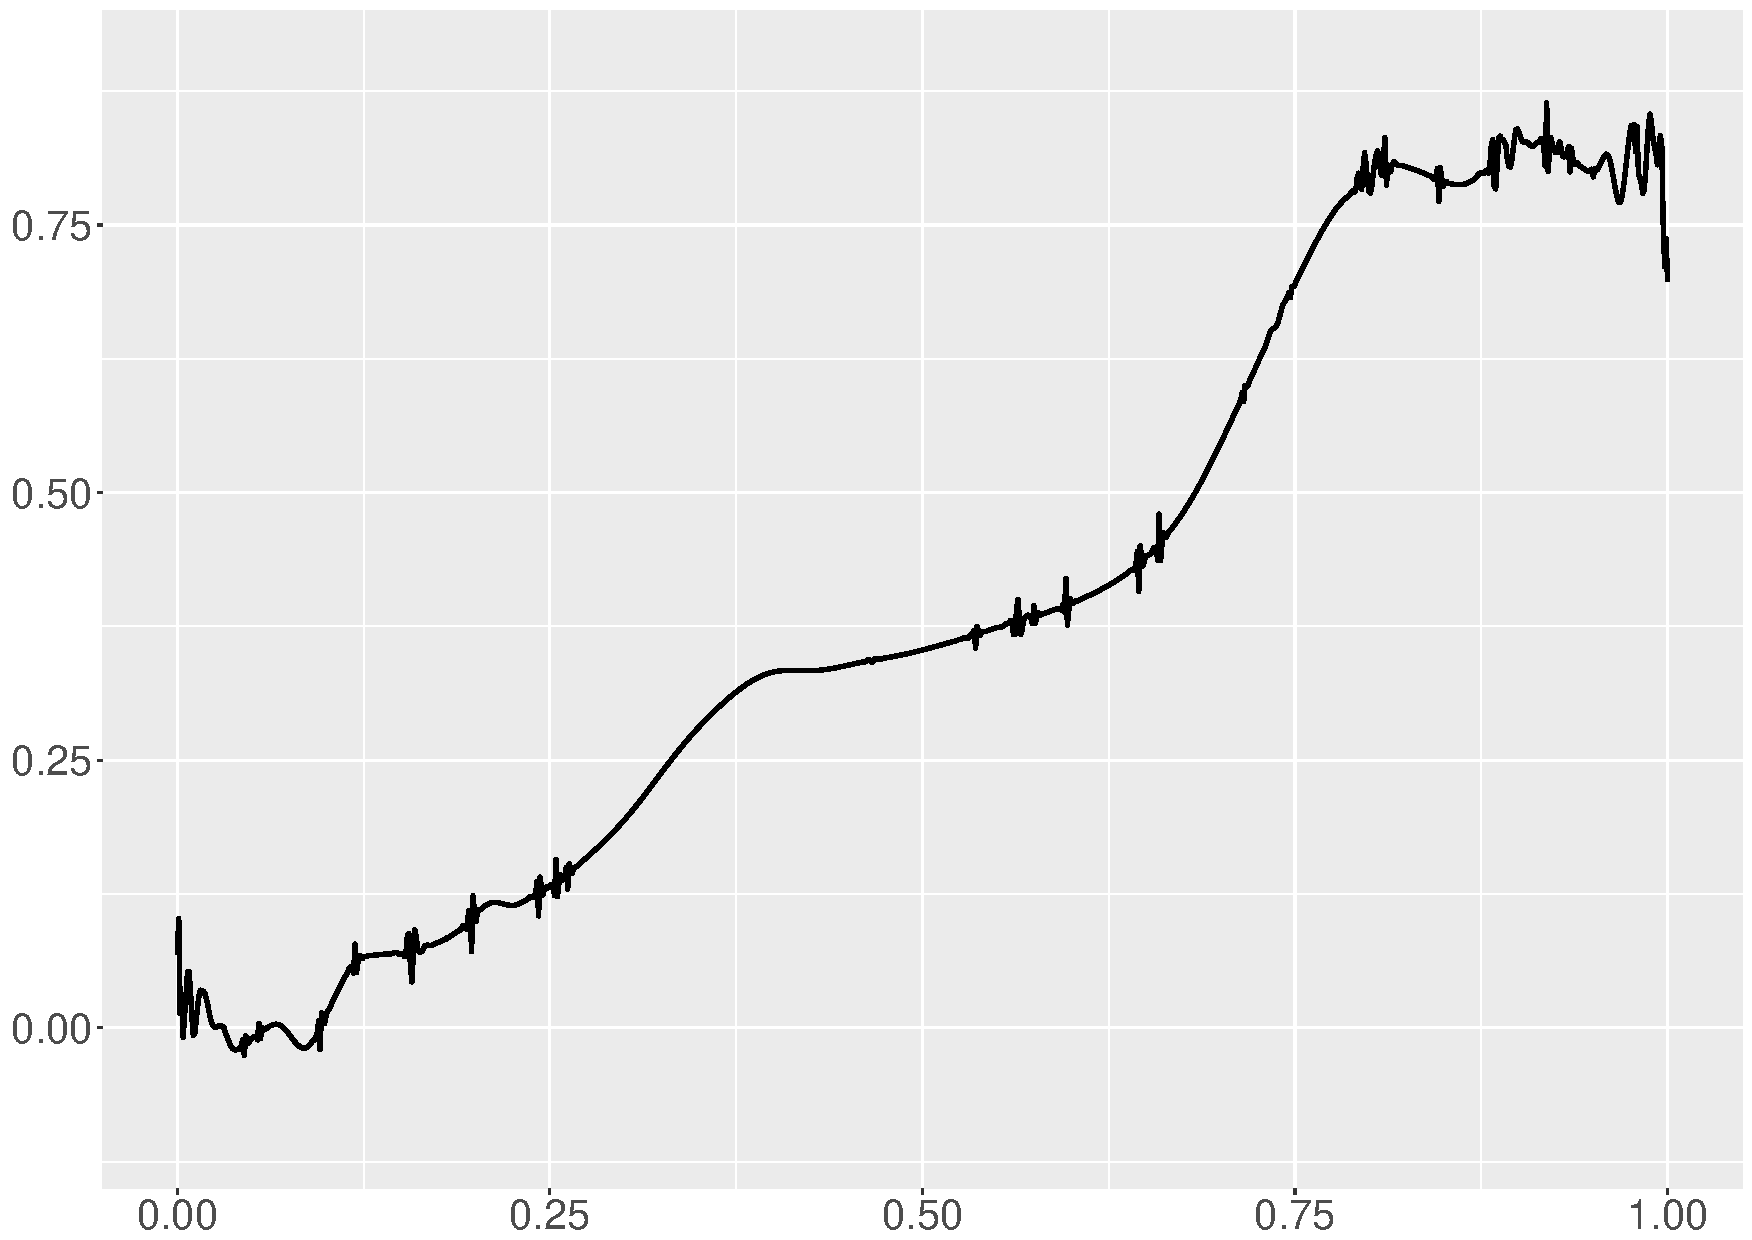
\includegraphics[width=\linewidth,height=0.45\textwidth]{Chapters/02TractorSplineTheory/plot/ggplot/ggBlocksSure.pdf}
    \caption{Reconstruction from Wavelet by sure threshold}
    \end{subfigure}
    \begin{subfigure}{0.45\textwidth}
    \centering
    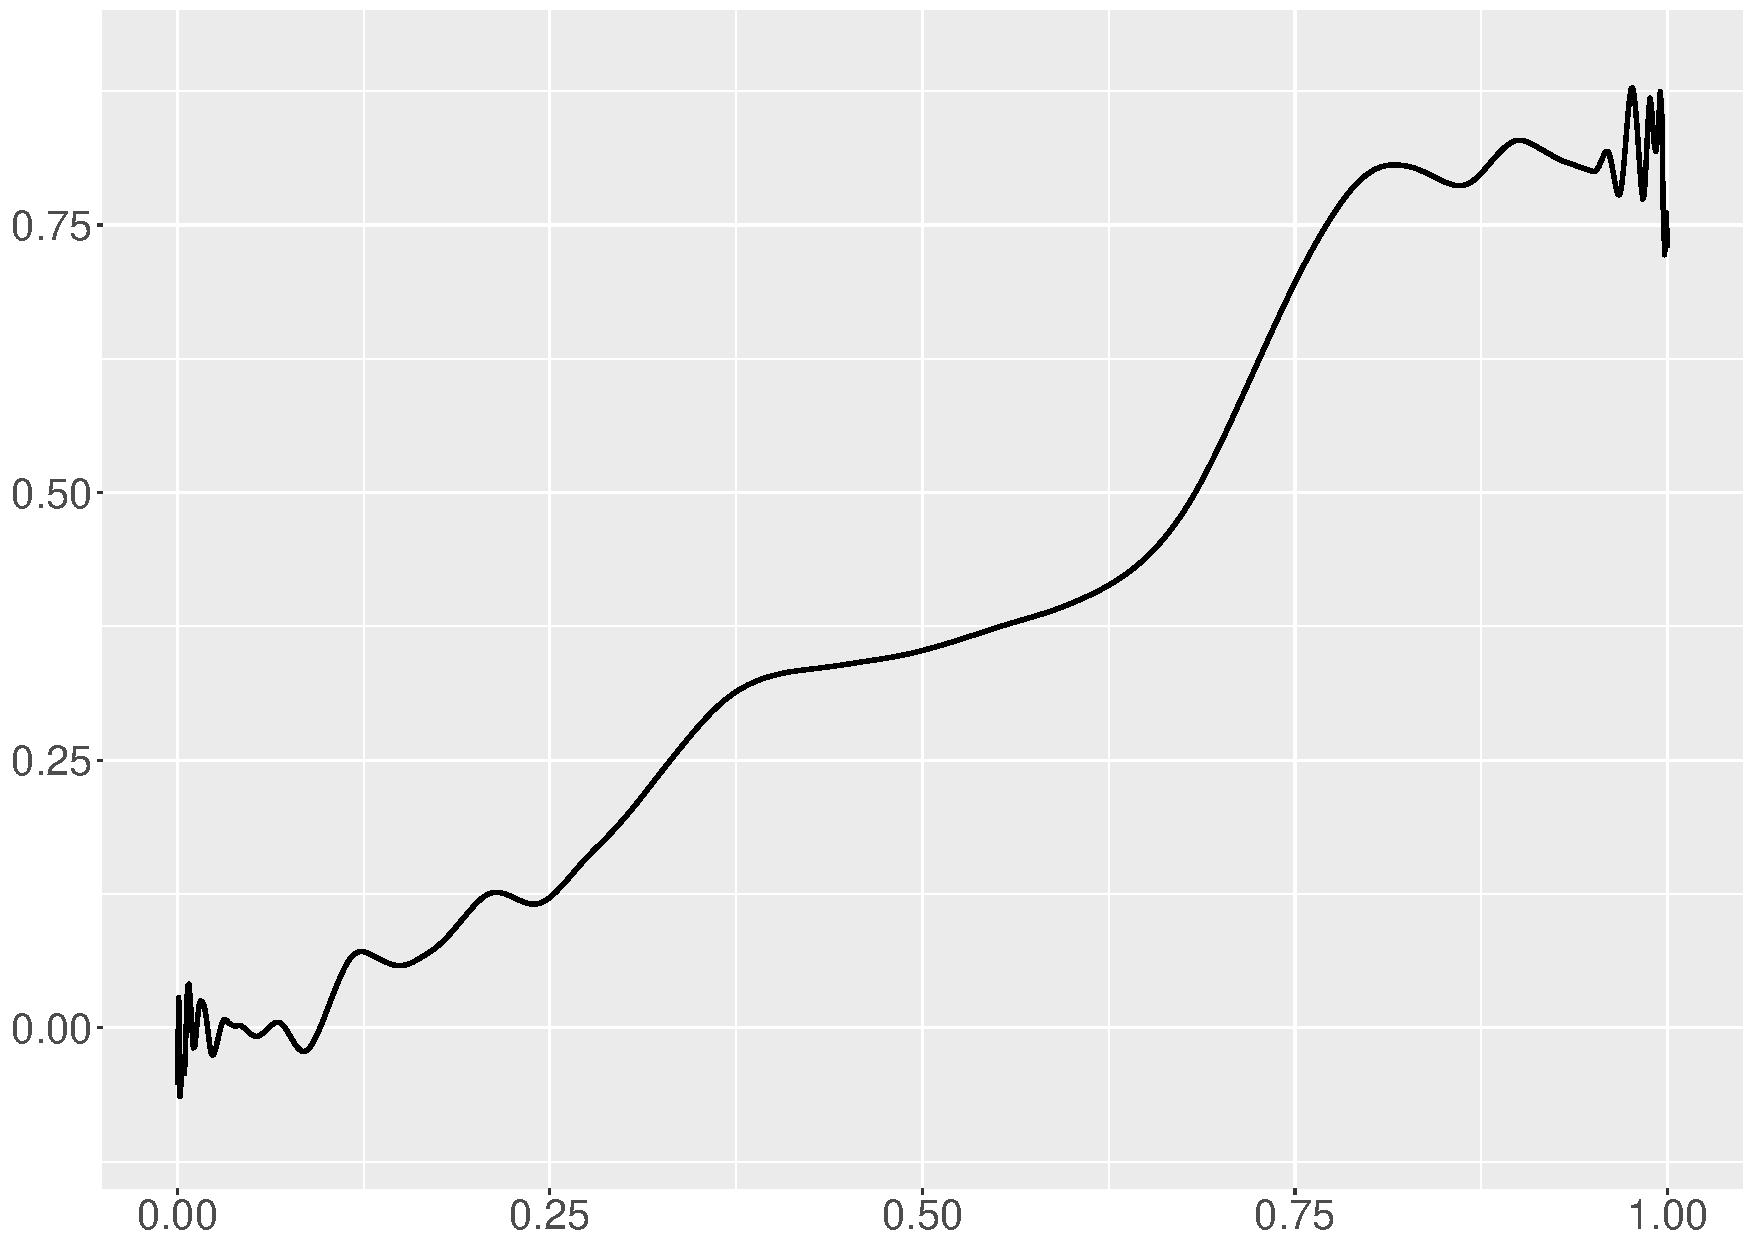
\includegraphics[width=\linewidth,height=0.45\textwidth]{Chapters/02TractorSplineTheory/plot/ggplot/ggBlocksBayes.pdf}
    \caption{Reconstruction from Wavelet by BayesThresh approach}
    \end{subfigure}
    \begin{subfigure}{0.45\textwidth}
    \centering
    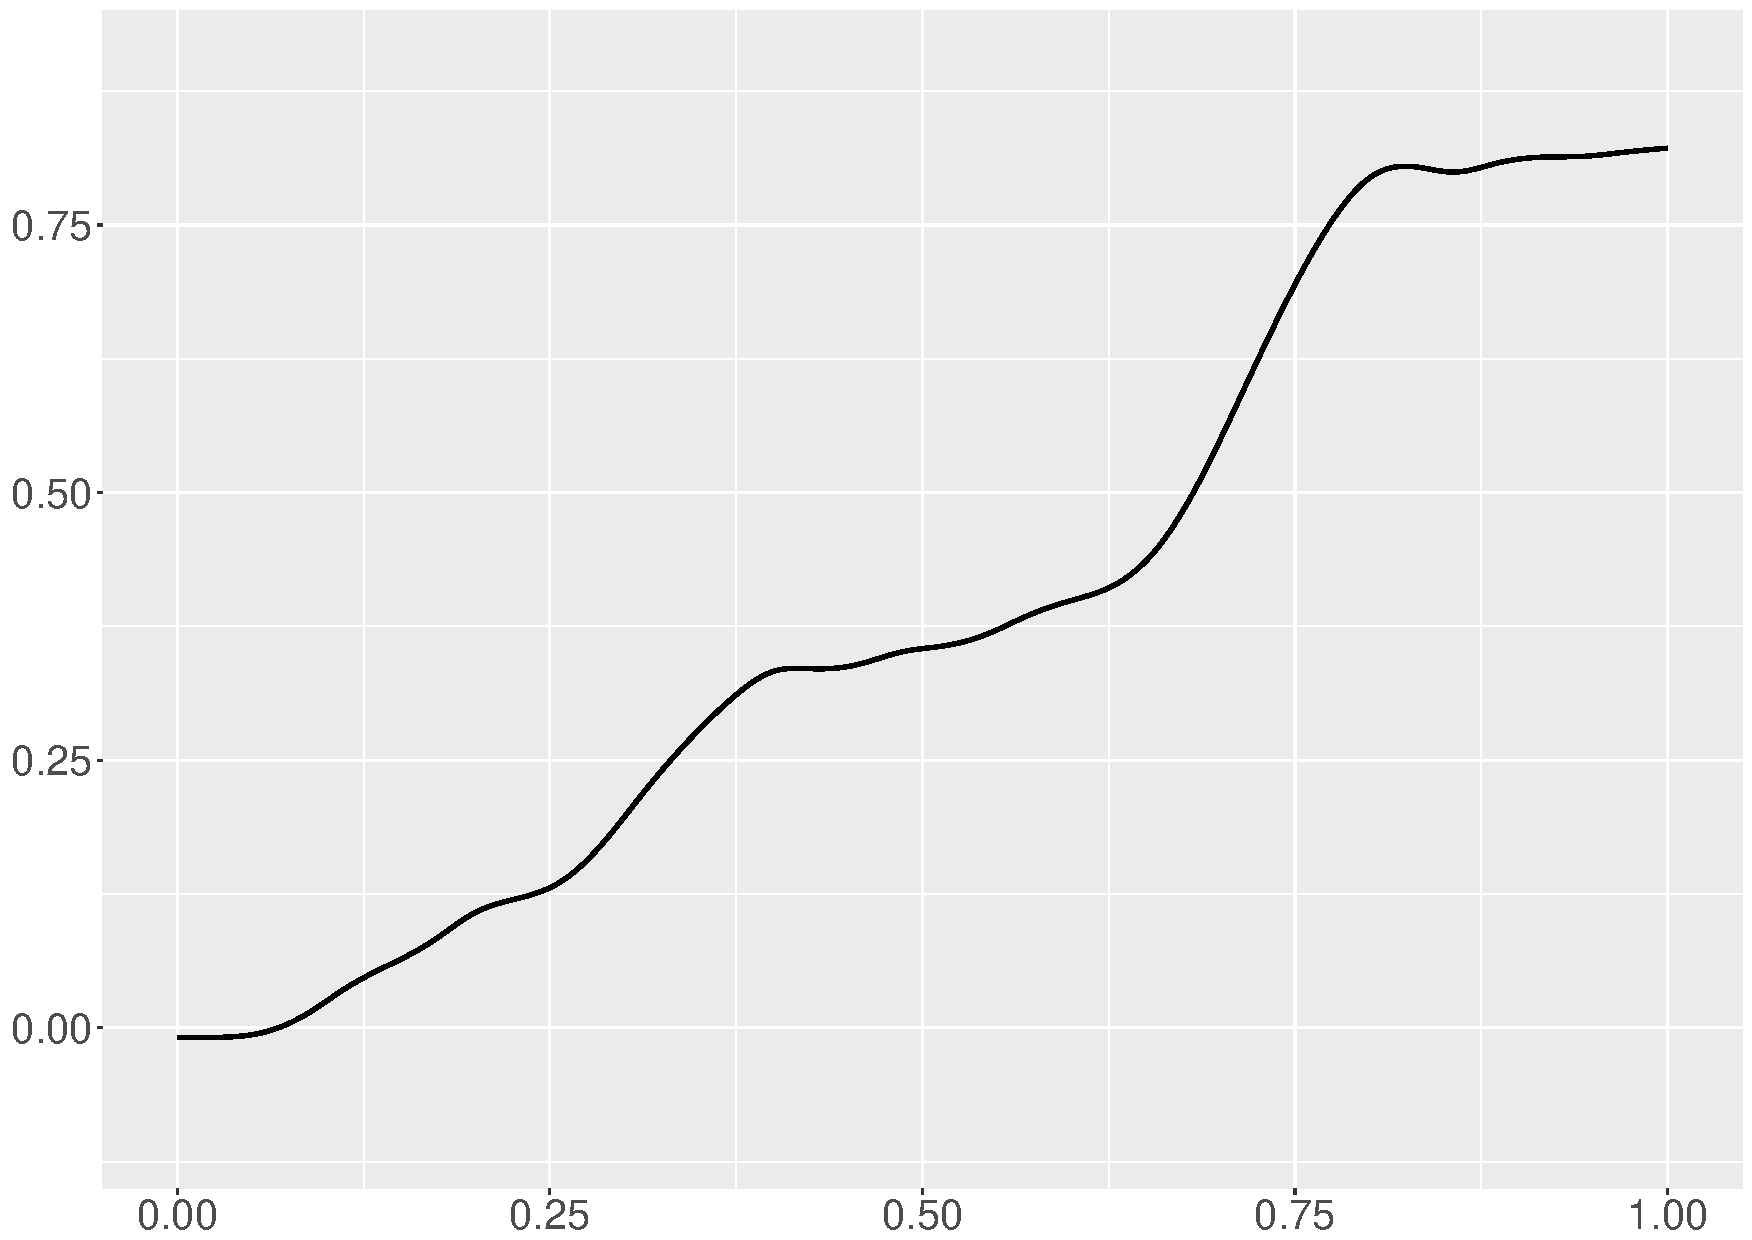
\includegraphics[width=\linewidth,height=0.45\textwidth]{Chapters/02TractorSplineTheory/plot/ggplot/ggBlocksPSpline.pdf}
    \caption{Reconstruction by P-spline \\\mbox{  } }
    \end{subfigure}
    \begin{subfigure}{0.45\textwidth}
    \centering
    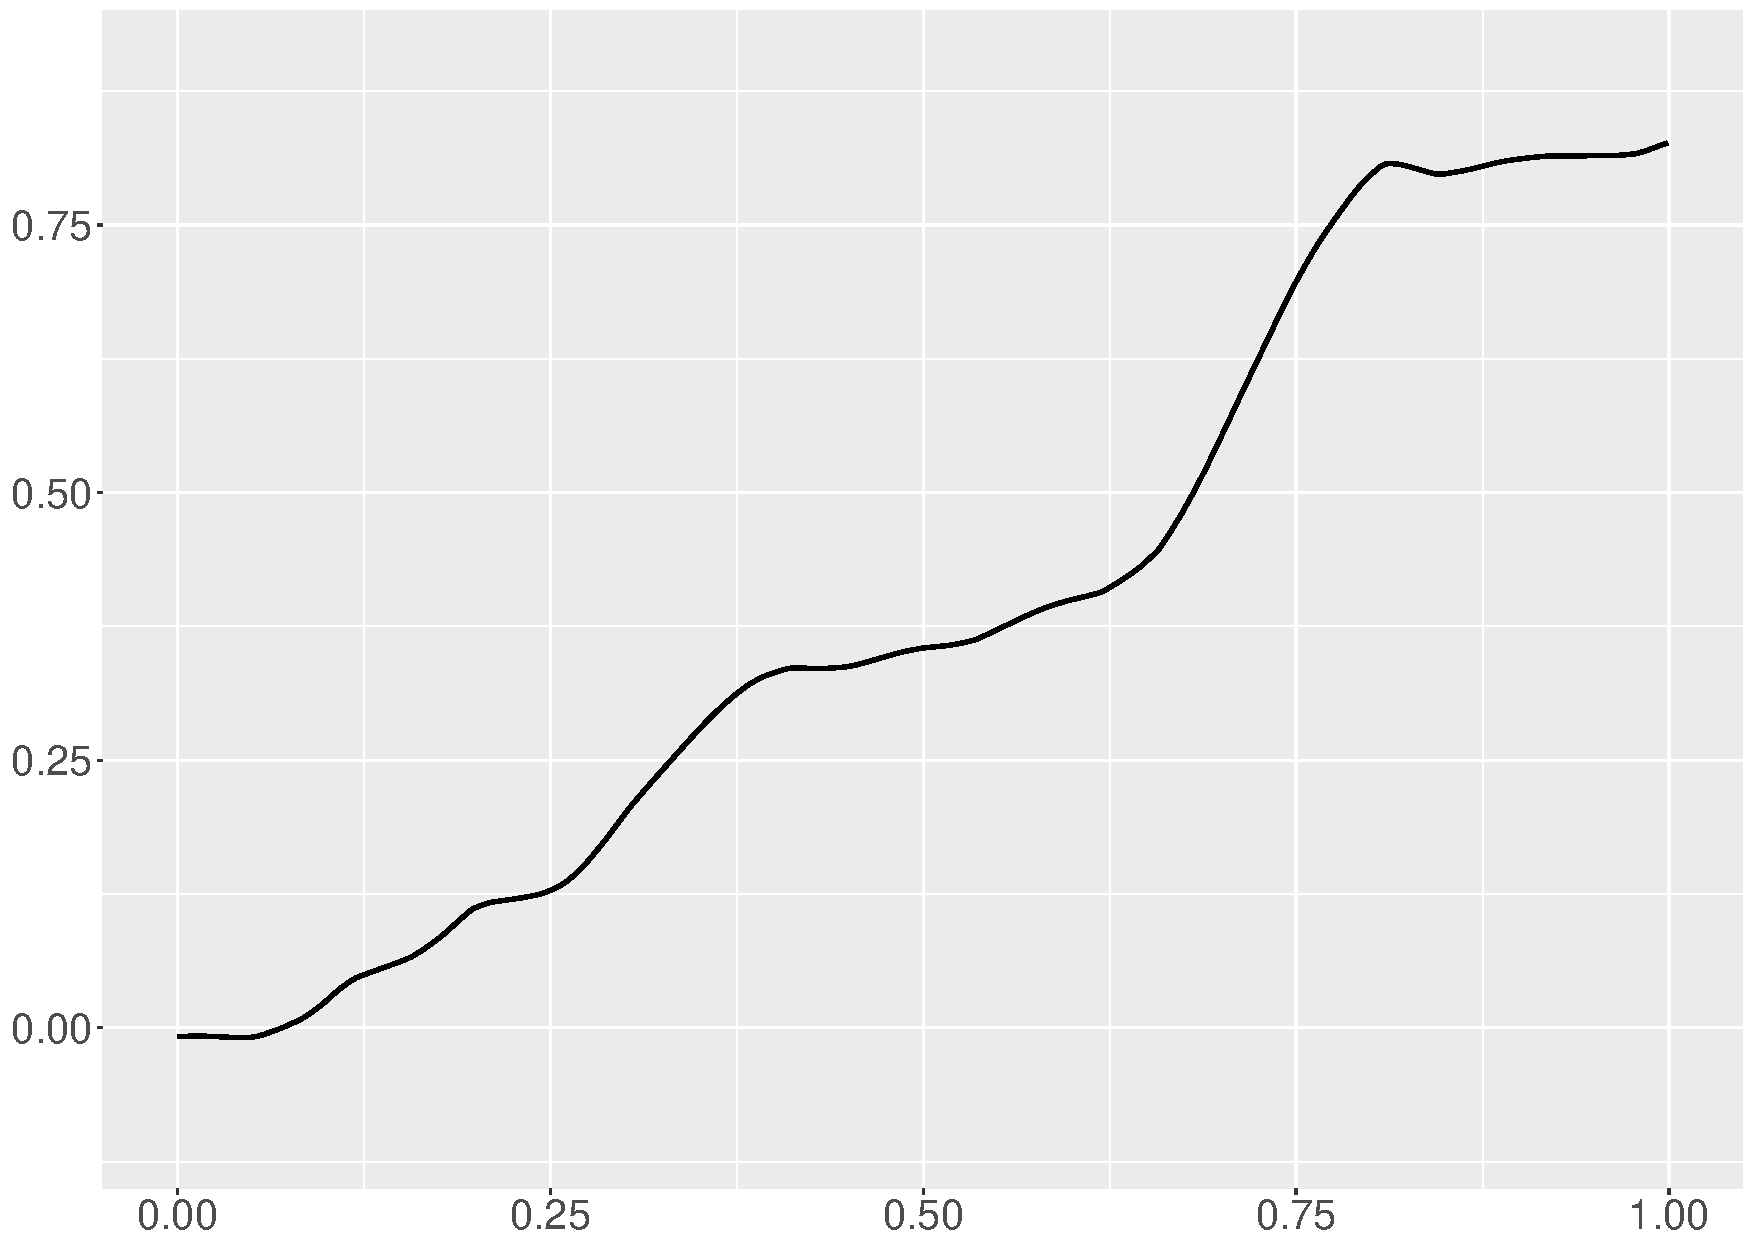
\includegraphics[width=\linewidth,height=0.45\textwidth]{Chapters/02TractorSplineTheory/plot/ggplot/ggBlocksGamma.pdf}
    \caption{Reconstruction by V-spline setting $\gamma=0$}
    \end{subfigure}
  \begin{subfigure}{0.45\textwidth}
    \centering
    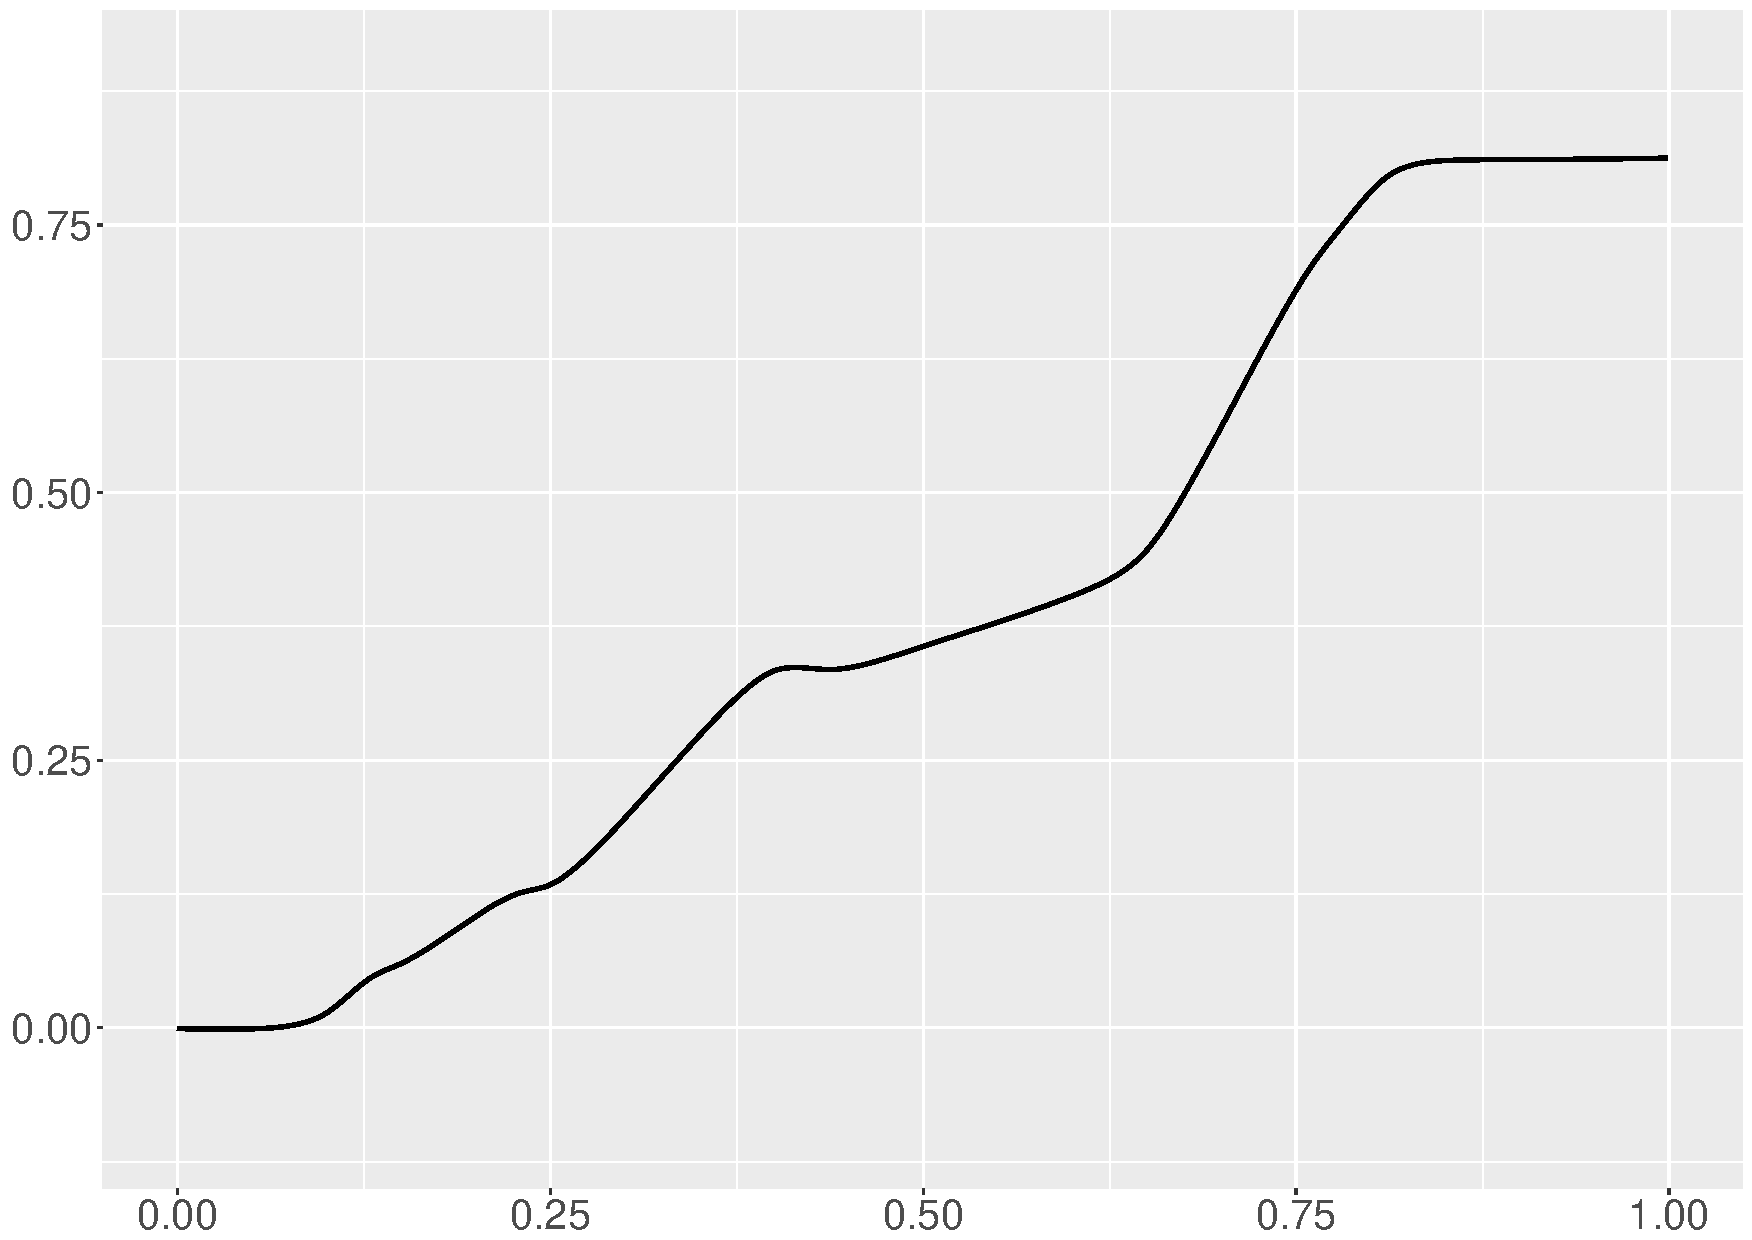
\includegraphics[width=\linewidth,height=0.45\textwidth]{Chapters/02TractorSplineTheory/plot/ggplot/ggBlocksTractorAPT.pdf}
    \caption{Reconstruction by V-spline with conventional penalty term}
    \end{subfigure}
    \begin{subfigure}{0.45\textwidth}
    \centering
    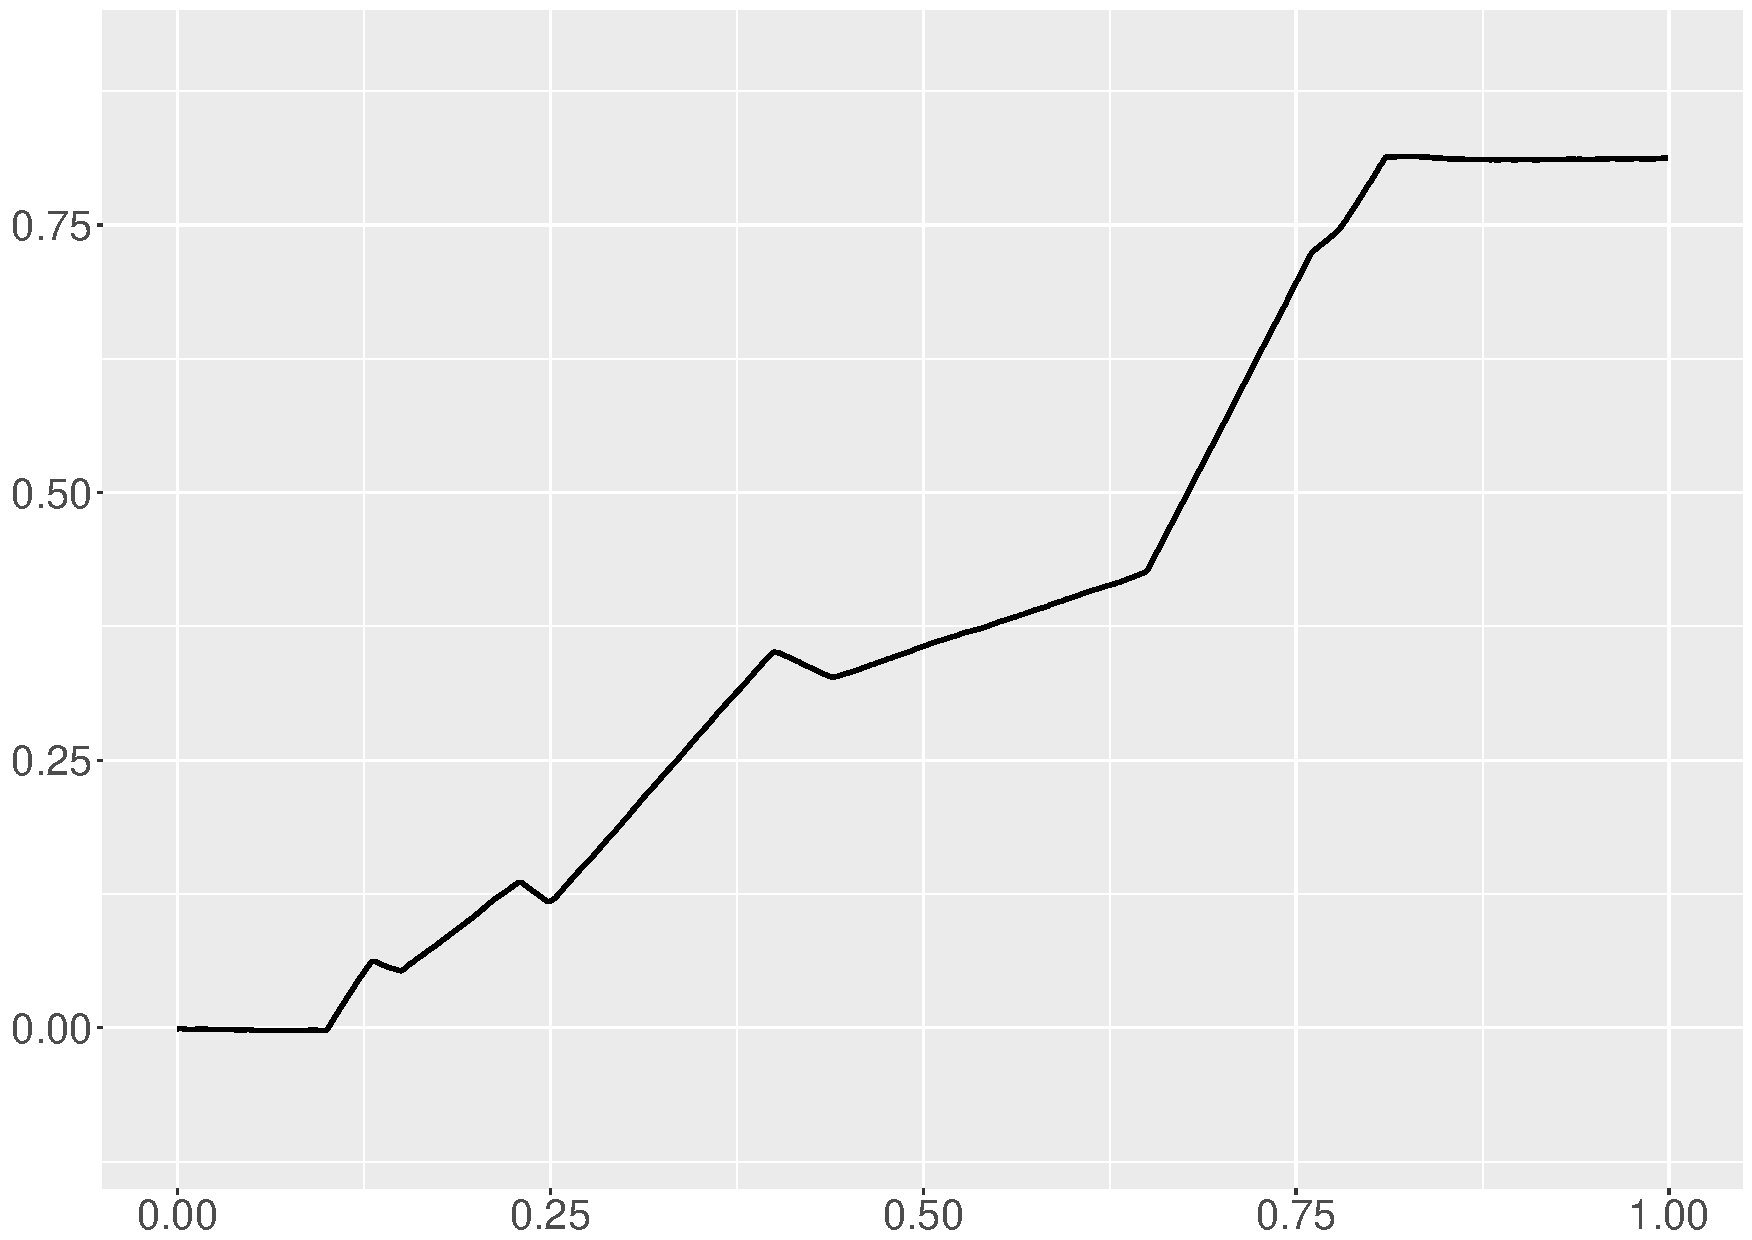
\includegraphics[width=\linewidth,height=0.45\textwidth]{Chapters/02TractorSplineTheory/plot/ggplot/ggBlocksTractor.pdf}
    \caption{Reconstruction by the proposed V-spline}
    \end{subfigure}
\caption{Numerical example: $\textit{Blocks}$. Comparison of different reconstruction methods with simulated data.}\label{num1}
 \end{figure}

%
%\begin{figure}
%  \centering
%    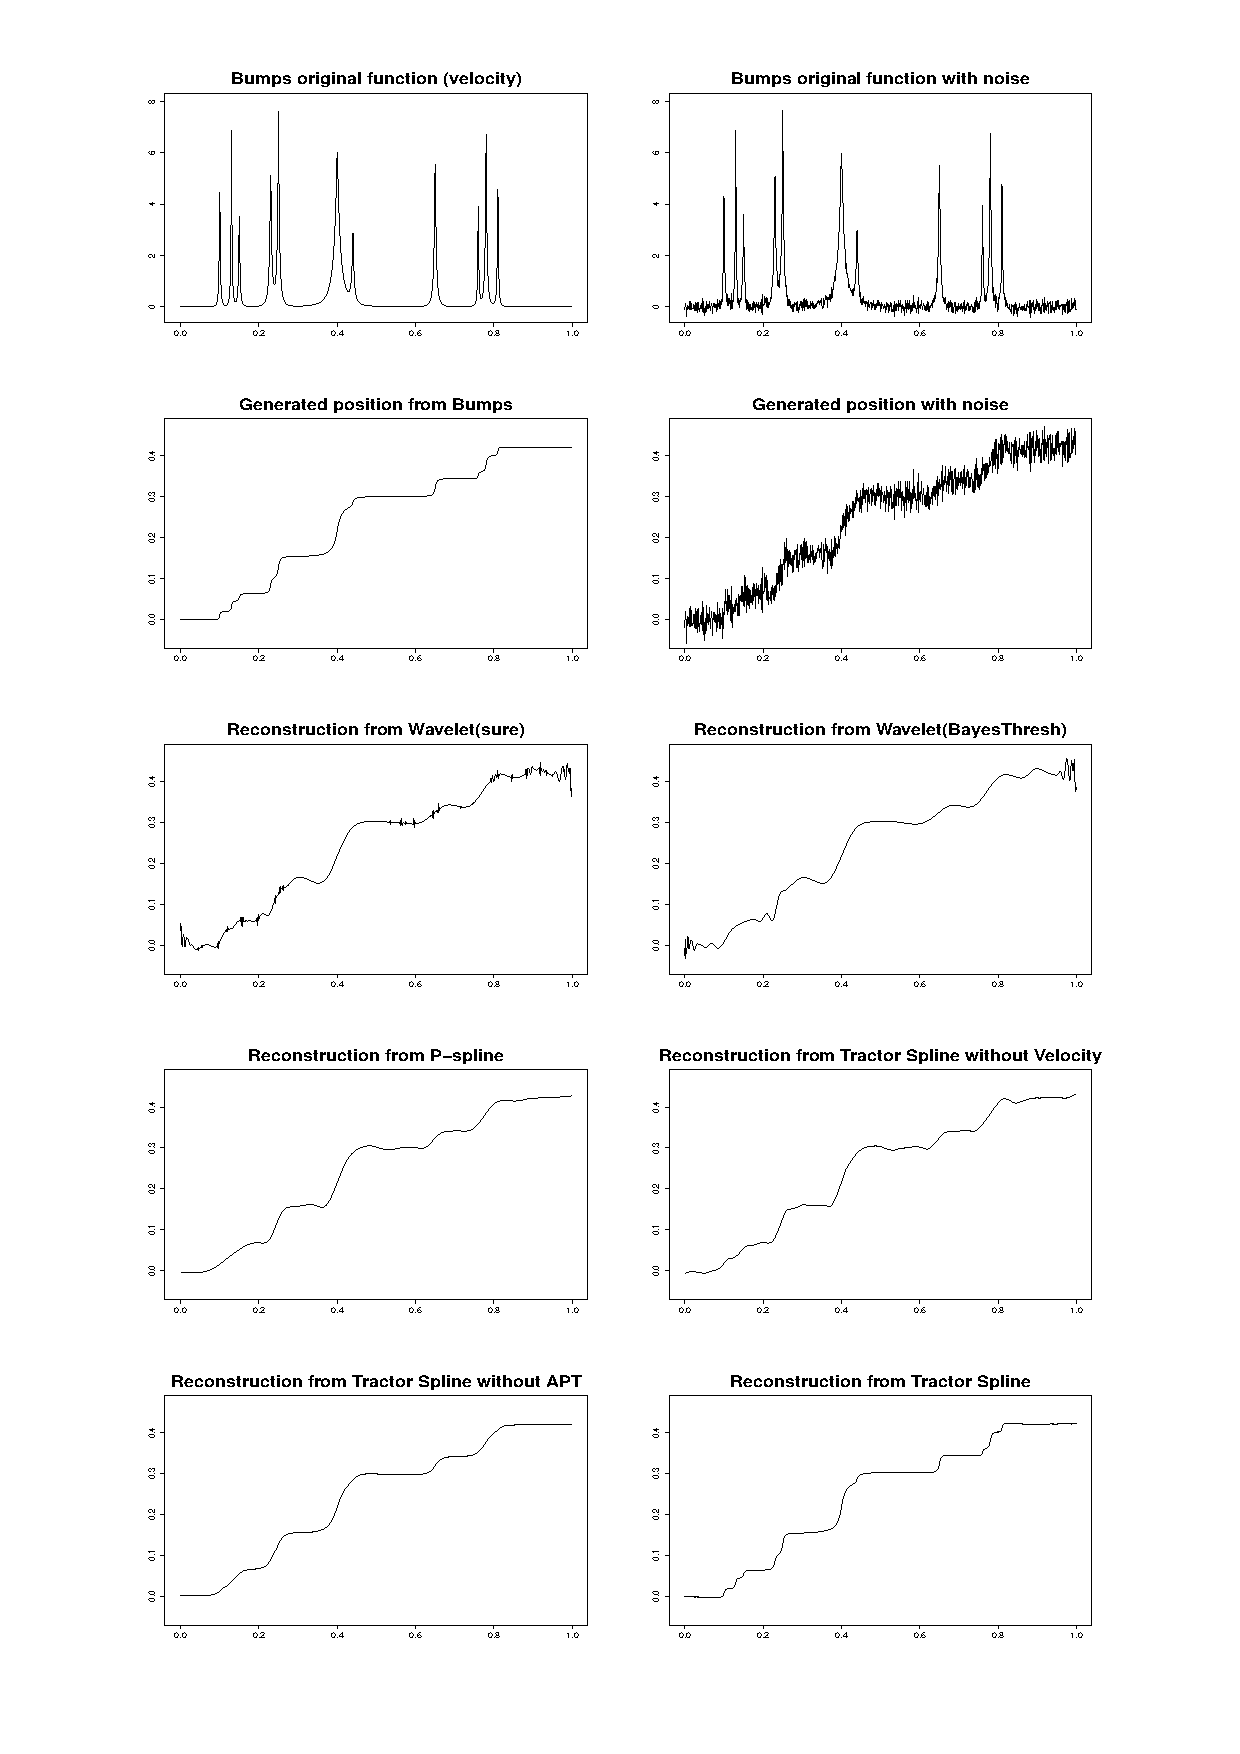
\includegraphics[width=\textwidth,height=14cm]{Chapters/02TractorSplineTheory/plot/bumps10}
%  \caption{Numerical example: $\textit{Bumps}$. (a) The true velocity function. (b) Velocity with Gaussian noise at SNR=7. (c) Generated position function. (d) Position with Gaussian noise at SNR=7. (e) Reconstruction from Wavelet with sure threshold. (f) Reconstruction from Wavelet with BayesThresh approach. (g) Reconstruction by P-spline. (h) Reconstruction by V-spline setting $\gamma=0$. (i) Reconstruction by V-spline with normal penalty term. (j) Reconstruction by proposed V-spline.}\label{num2}
%\end{figure}


\begin{figure}
    \centering
    \begin{subfigure}{0.45\textwidth}
    \centering
    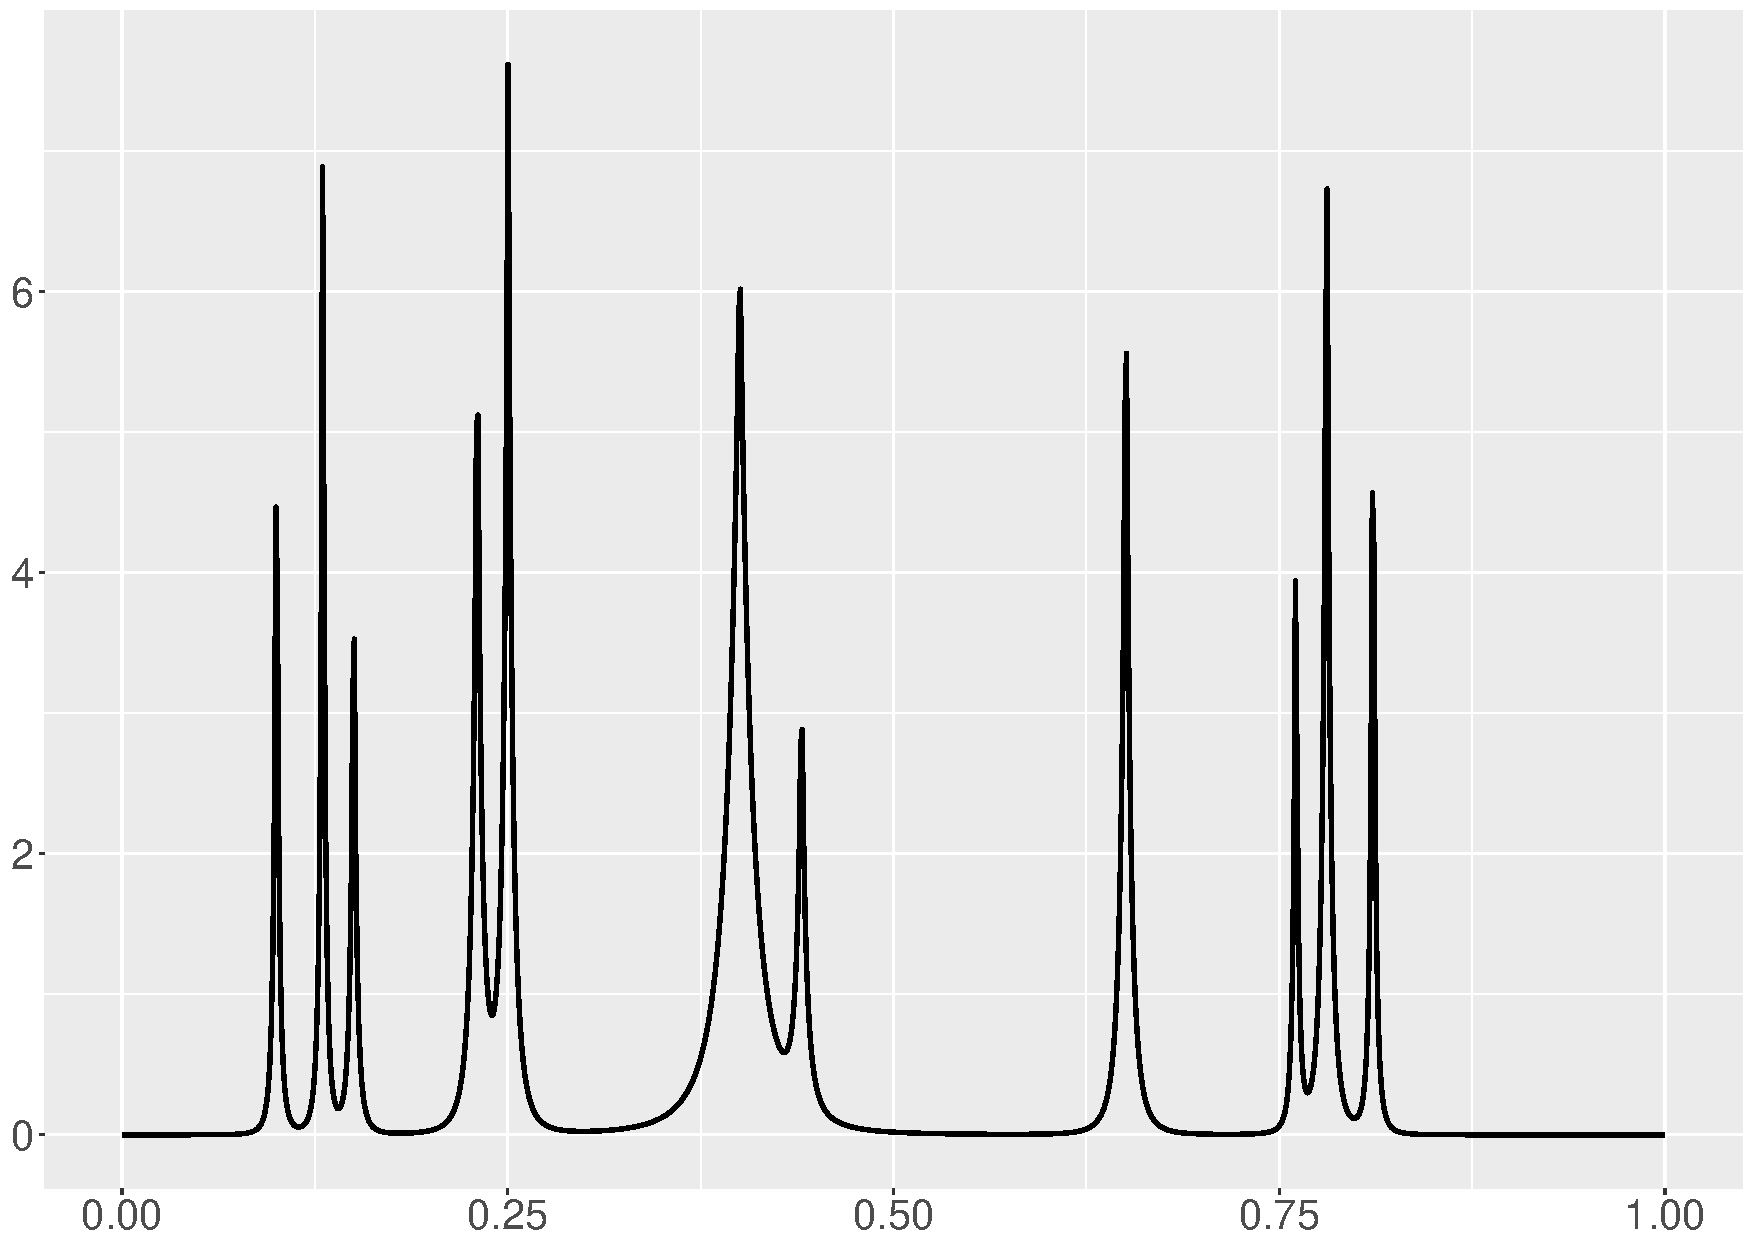
\includegraphics[width=\linewidth,height=0.45\textwidth]{Chapters/02TractorSplineTheory/plot/ggplot/ggBumps.pdf}
    \caption{True \textit{Bumps} function}
    \end{subfigure}%
    \begin{subfigure}{0.45\textwidth}
    \centering
    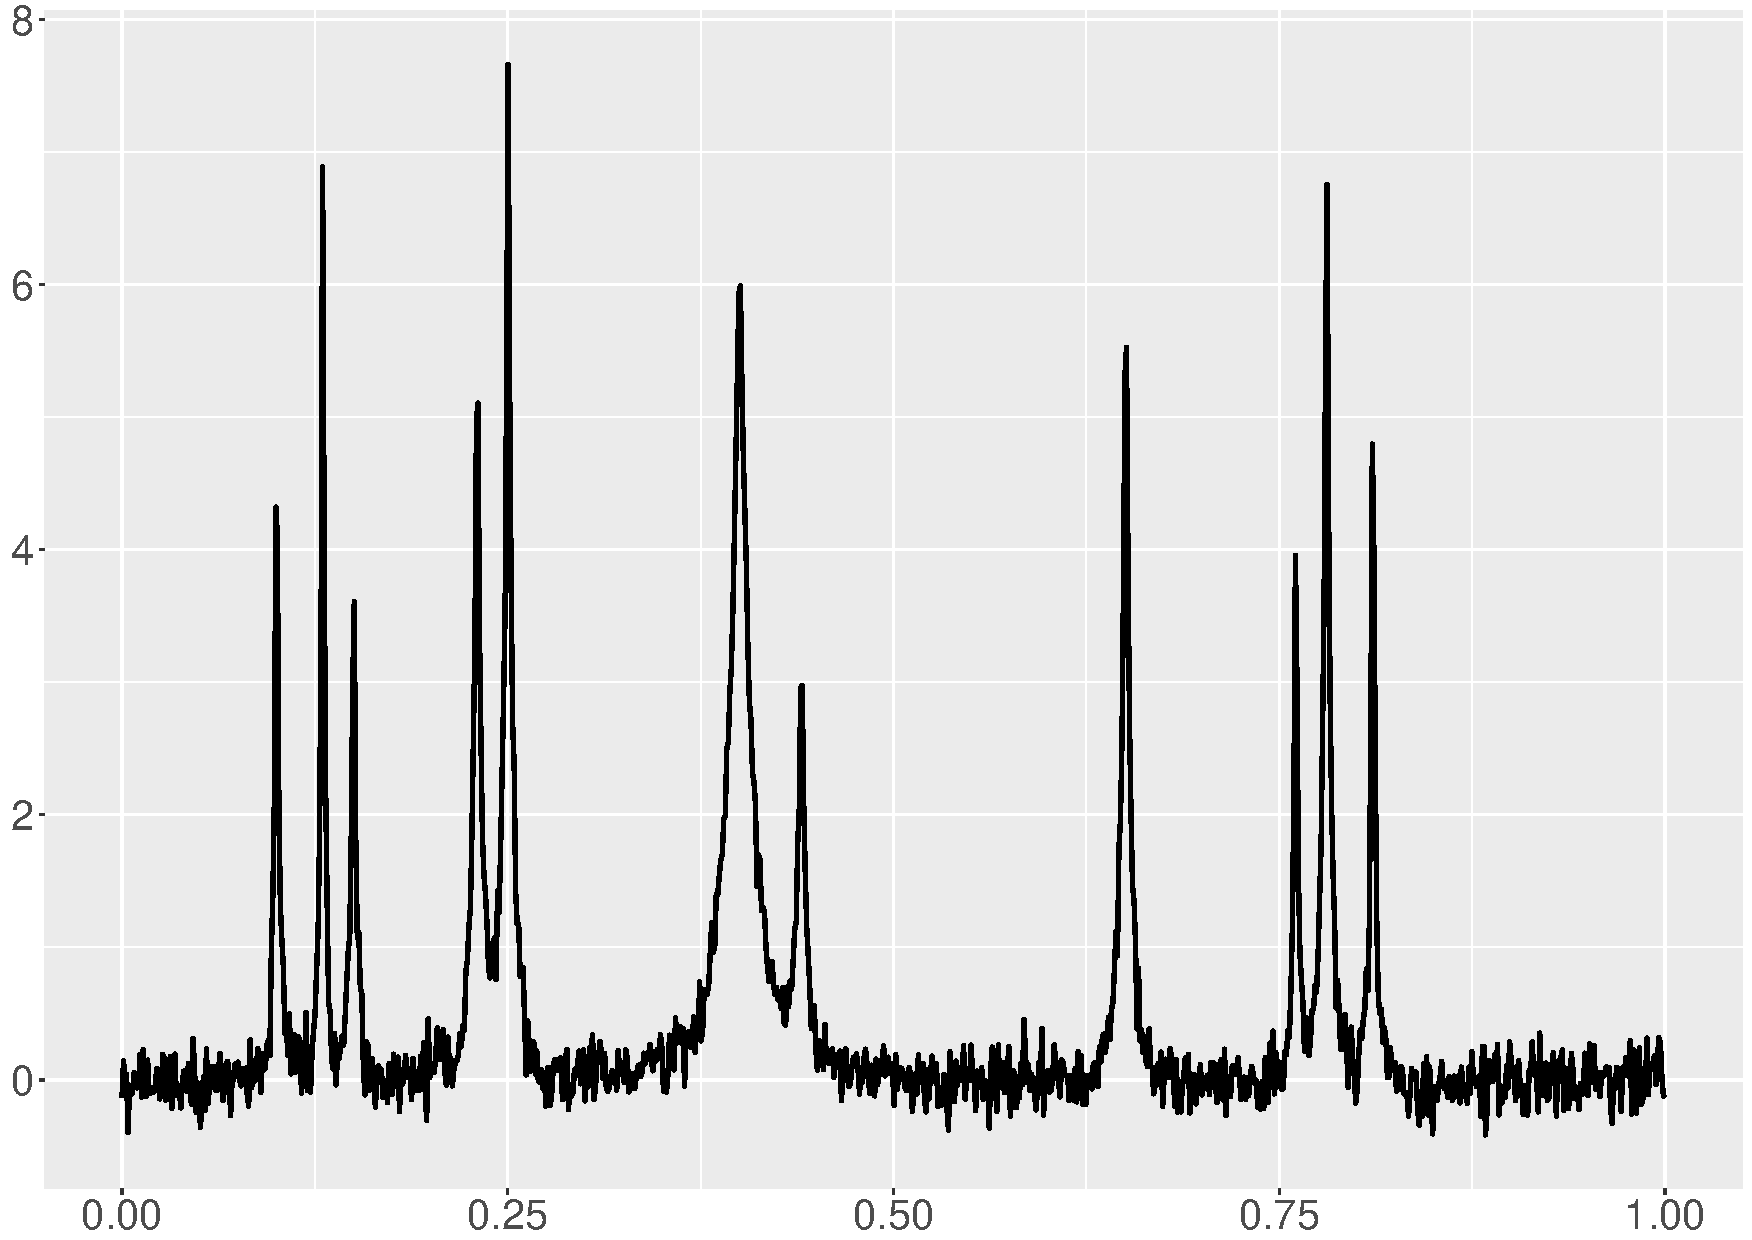
\includegraphics[width=\linewidth,,height=0.45\textwidth]{Chapters/02TractorSplineTheory/plot/ggplot/ggBumpsNoise.pdf}
    \caption{Noisy \textit{Bumps} at \textit{SNR}=7}
    \end{subfigure}
    \begin{subfigure}{0.45\textwidth}
    \centering
    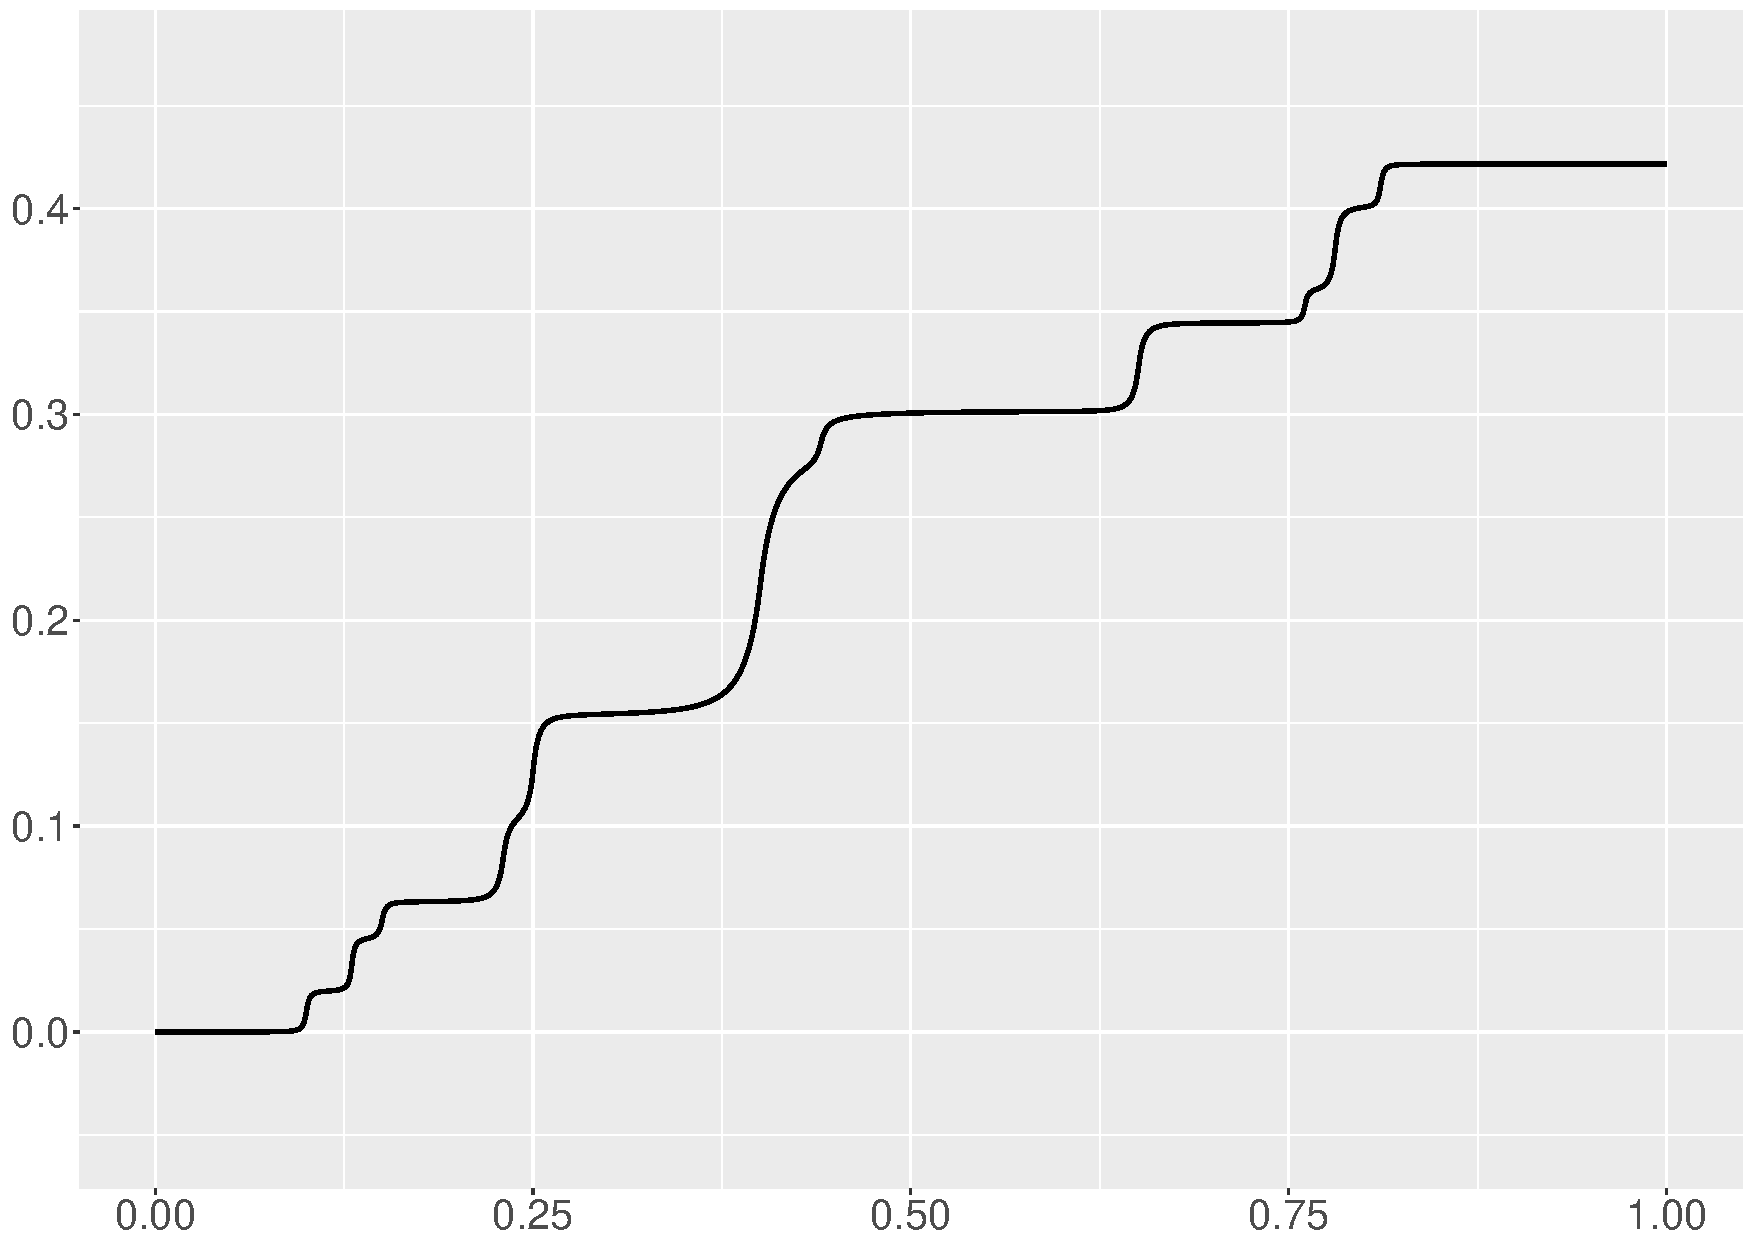
\includegraphics[width=\linewidth,height=0.45\textwidth]{Chapters/02TractorSplineTheory/plot/ggplot/ggBumpsPosition.pdf}
    \caption{Generated positions}
    \end{subfigure}
    \begin{subfigure}{0.45\textwidth}
    \centering
    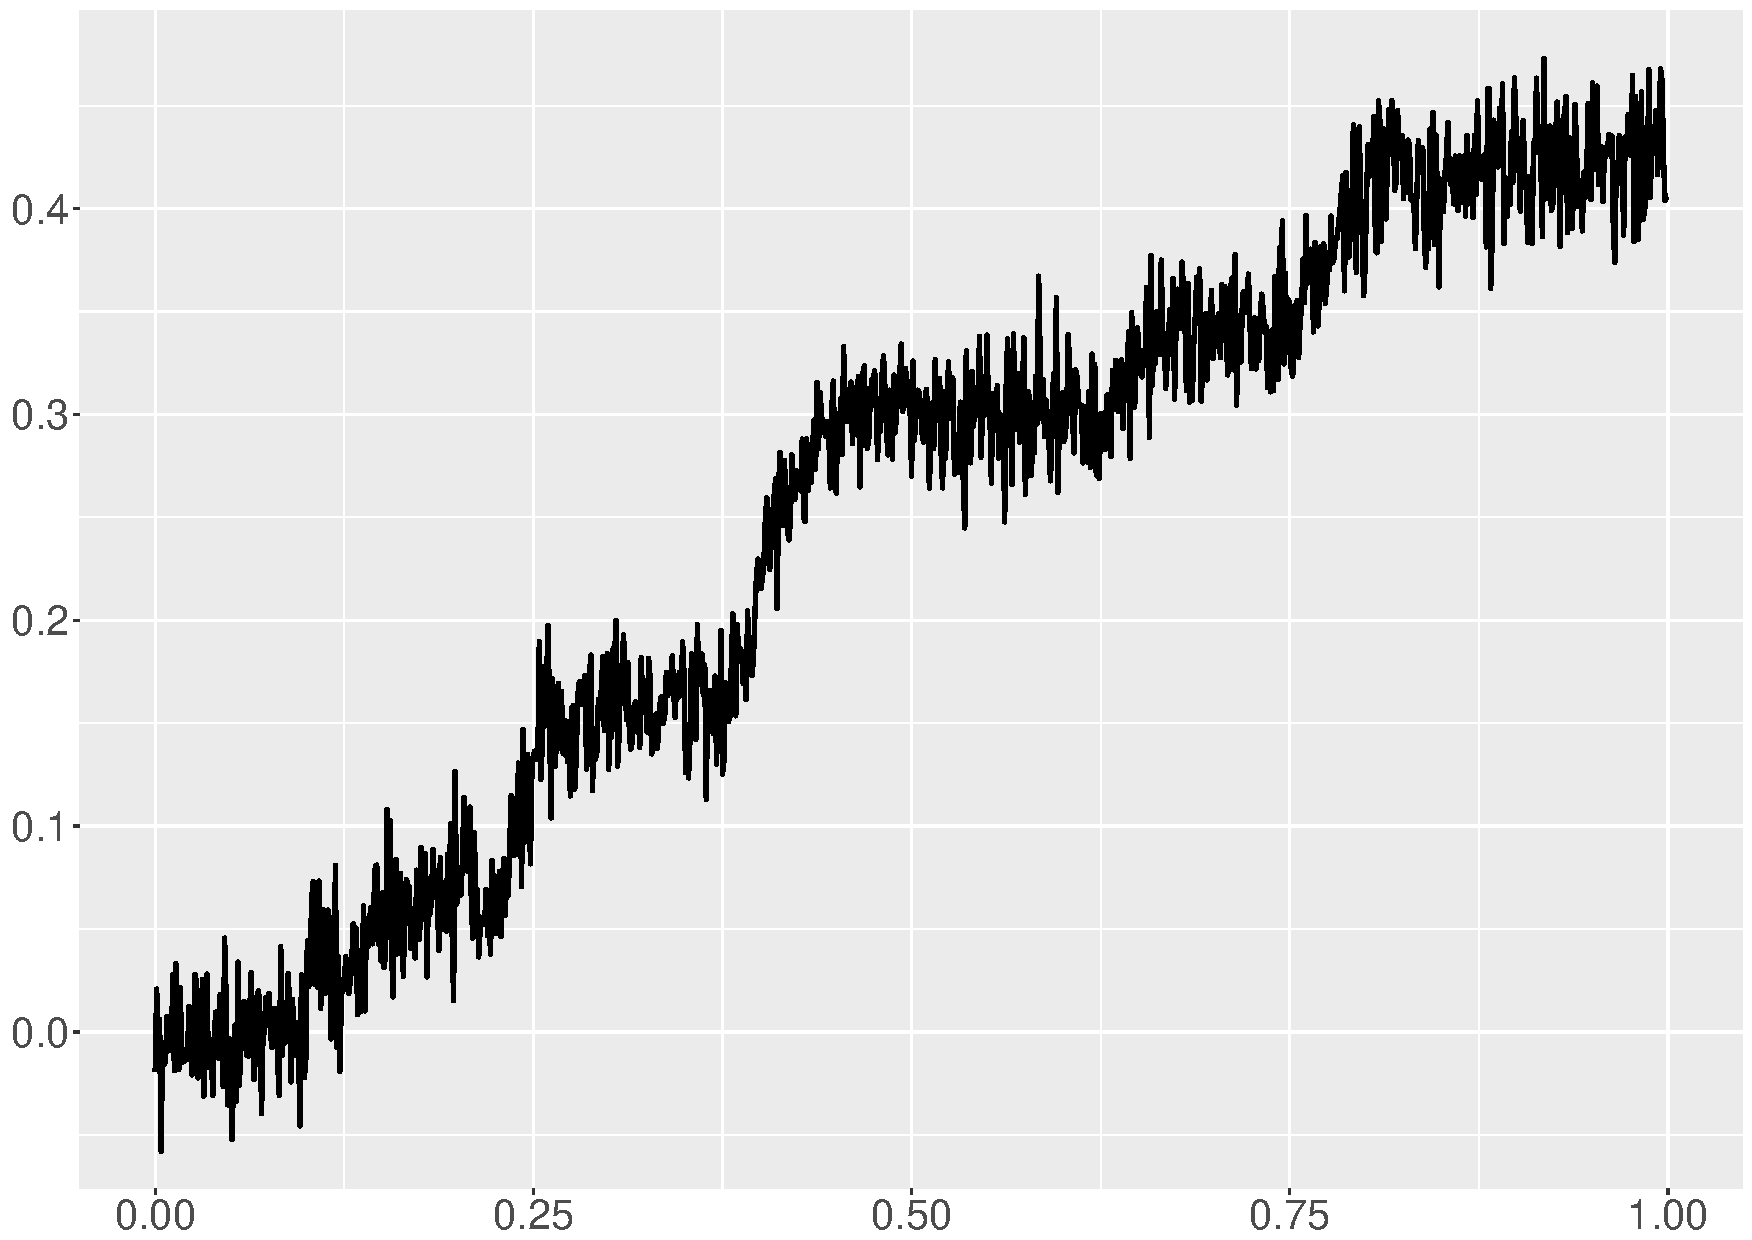
\includegraphics[width=\linewidth,height=0.45\textwidth]{Chapters/02TractorSplineTheory/plot/ggplot/ggBumpsPositionNoise.pdf}
    \caption{Noisy position at \textit{SNR}=7}
    \end{subfigure}
    \begin{subfigure}{0.45\textwidth}
    \centering
    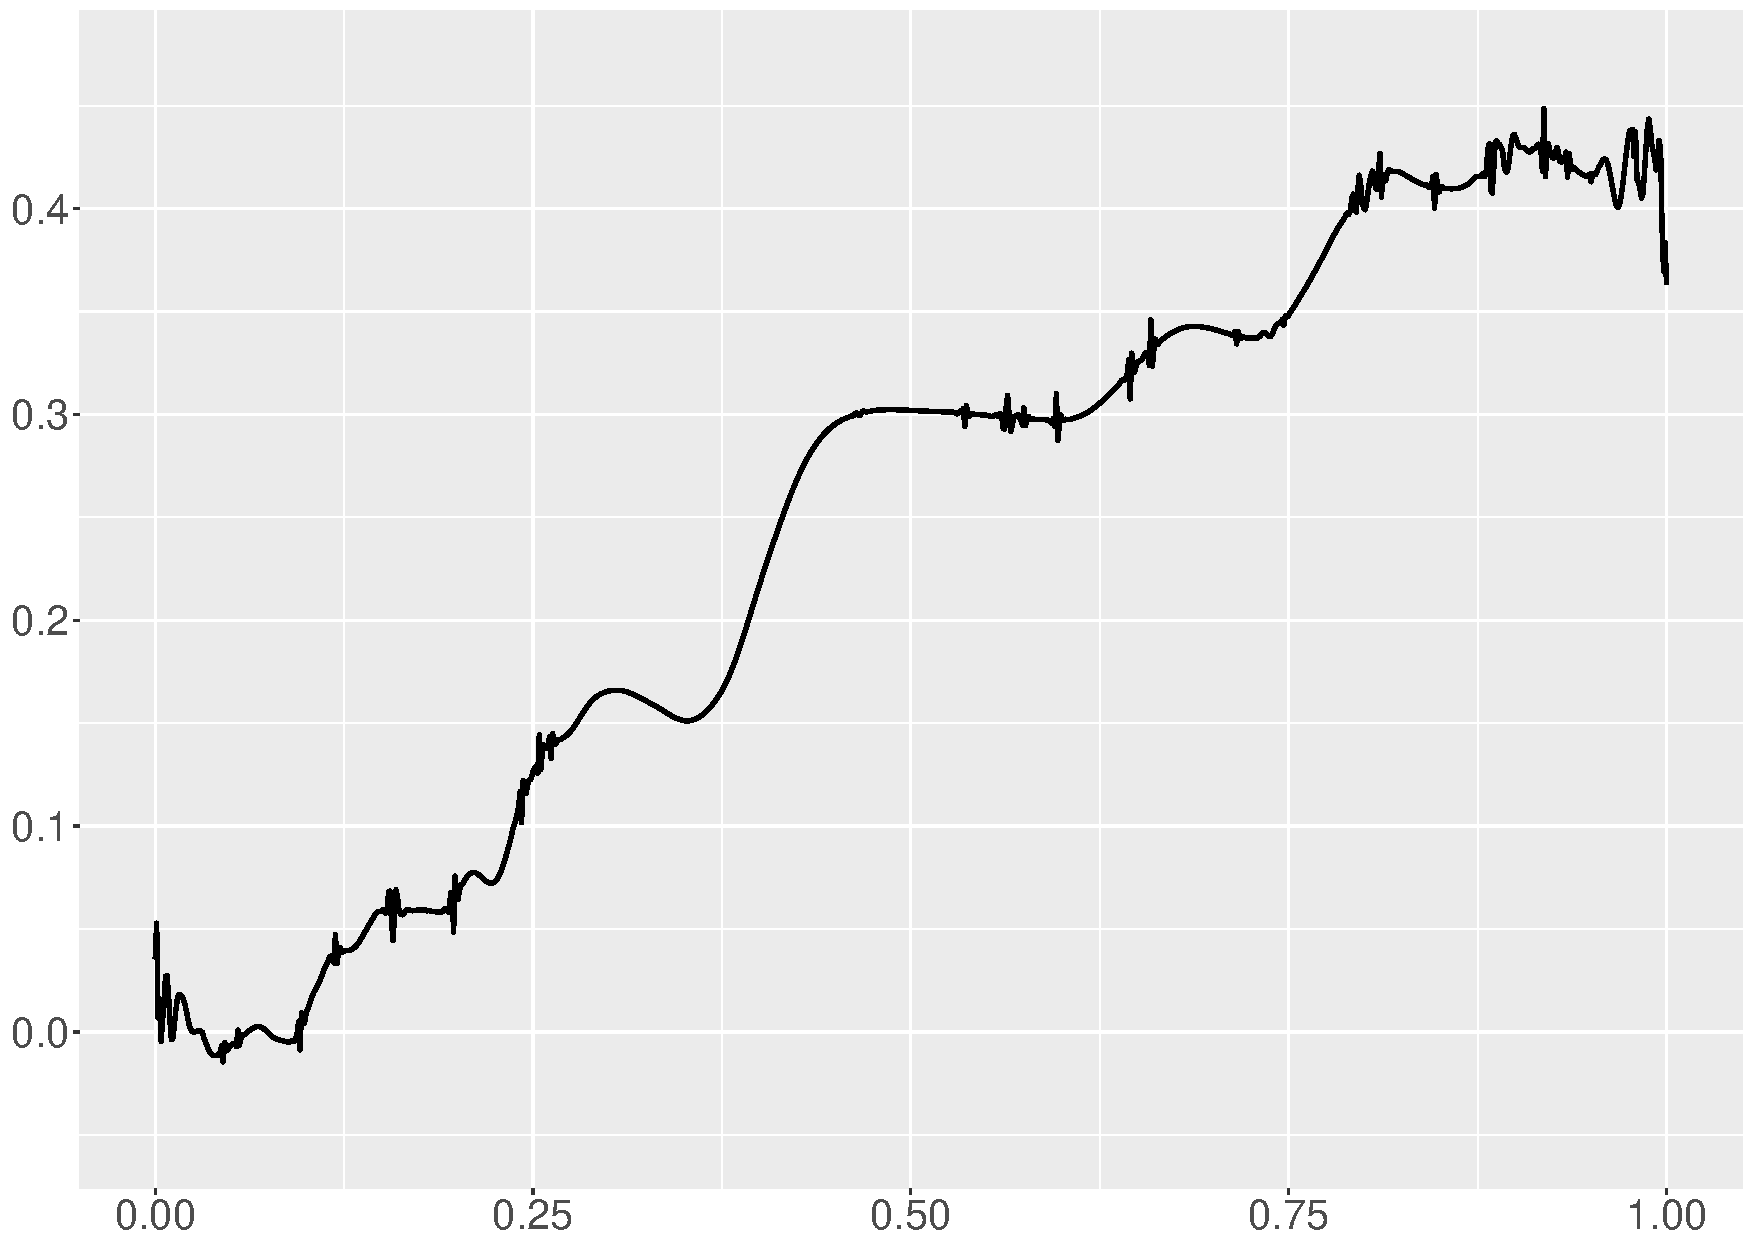
\includegraphics[width=\linewidth,height=0.45\textwidth]{Chapters/02TractorSplineTheory/plot/ggplot/ggBumpsSure.pdf}
    \caption{Reconstruction from Wavelet by sure threshold}
    \end{subfigure}
    \begin{subfigure}{0.45\textwidth}
    \centering
    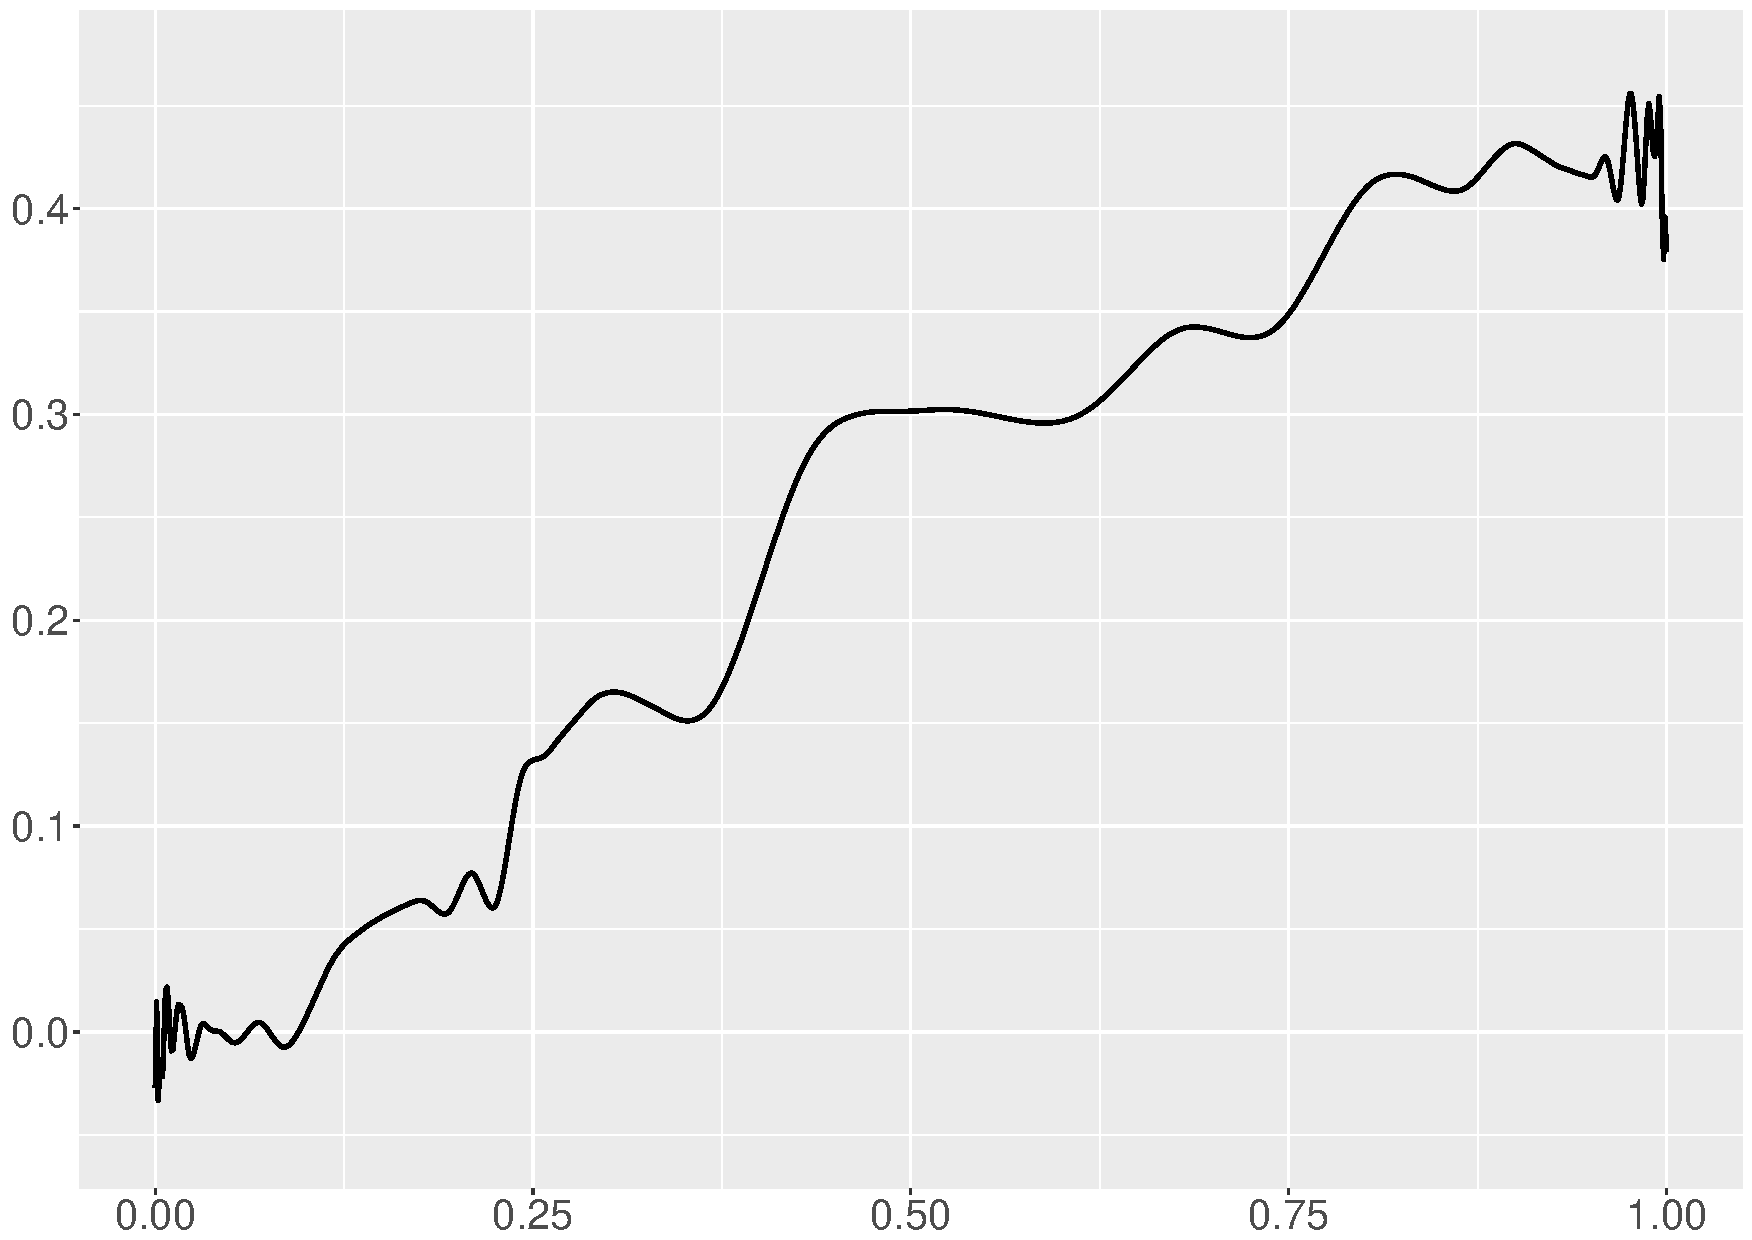
\includegraphics[width=\linewidth,height=0.45\textwidth]{Chapters/02TractorSplineTheory/plot/ggplot/ggBumpsBayes.pdf}
    \caption{Reconstruction from Wavelet by BayesThresh approach}
    \end{subfigure}
    \begin{subfigure}{0.45\textwidth}
    \centering
    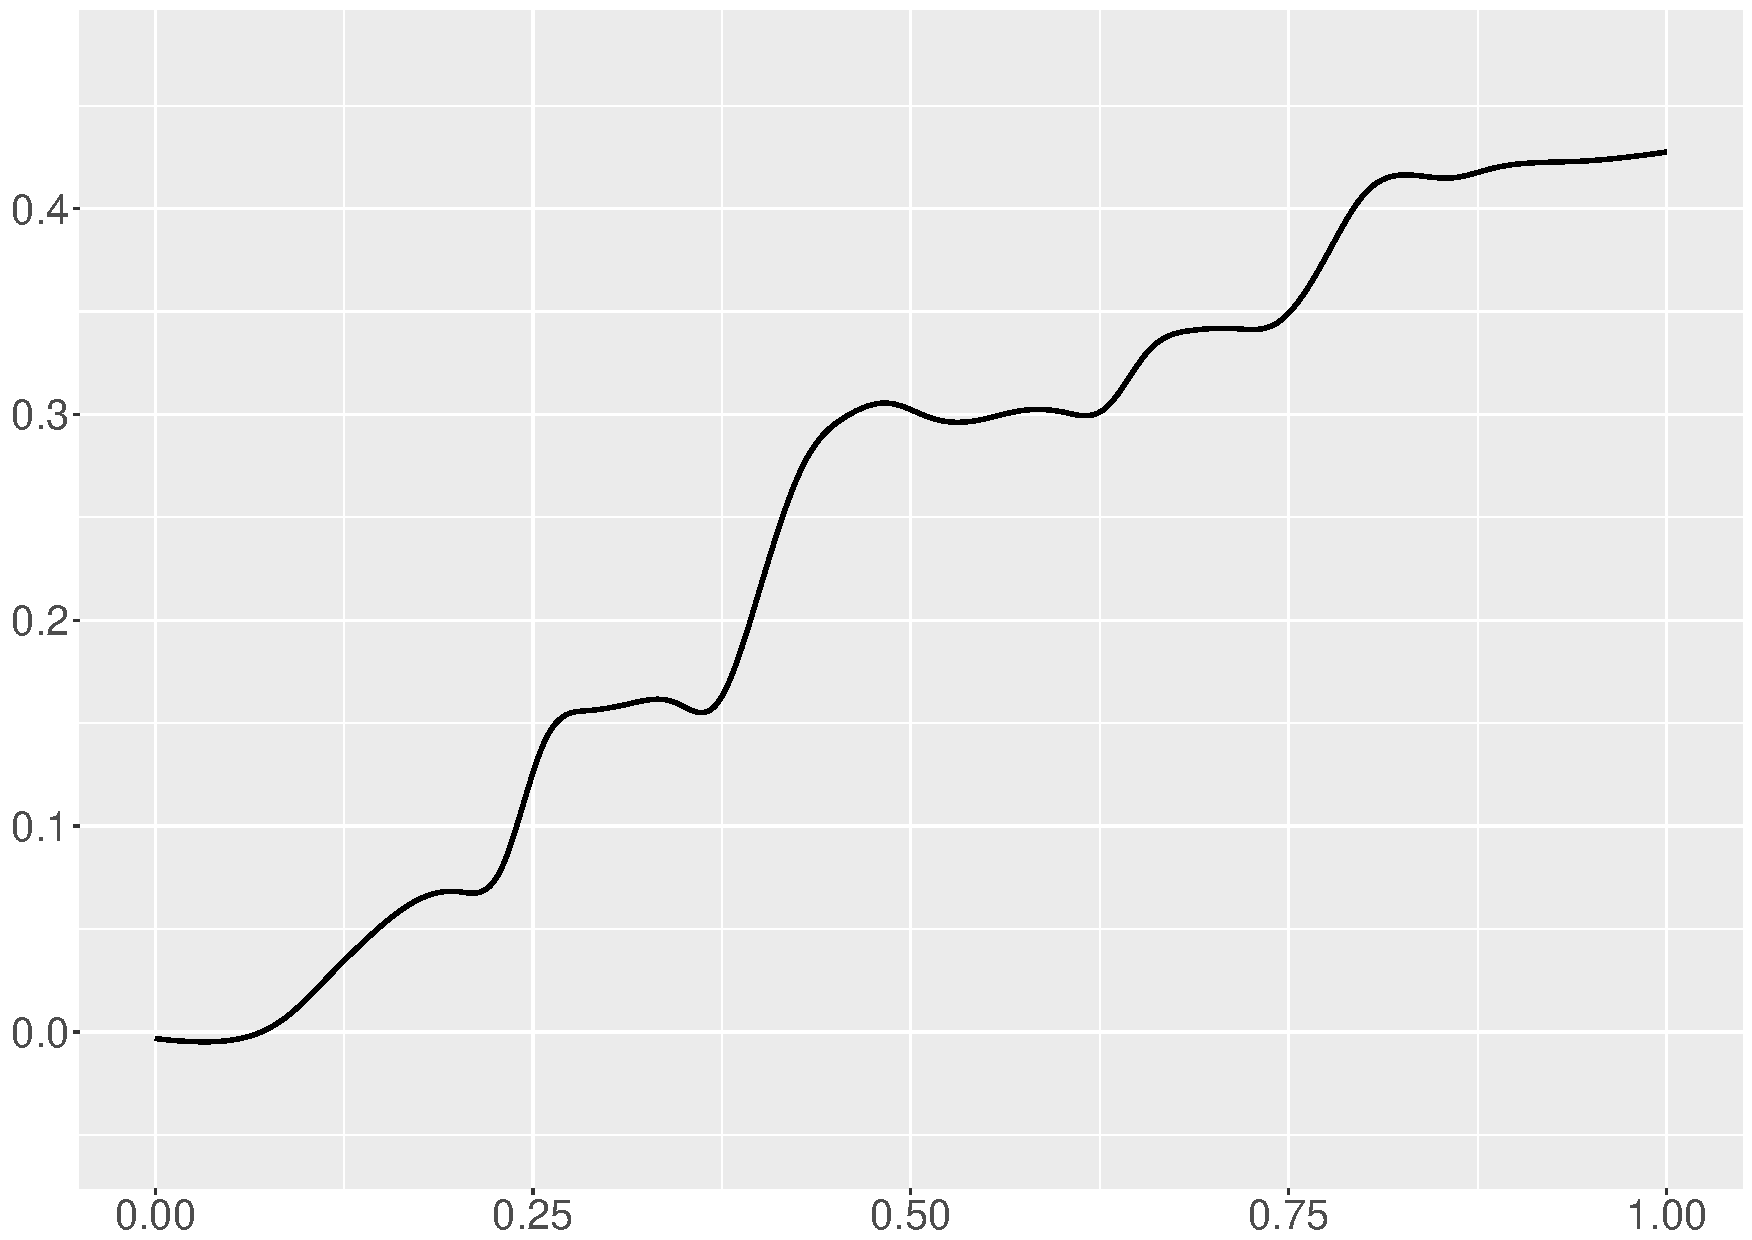
\includegraphics[width=\linewidth,height=0.45\textwidth]{Chapters/02TractorSplineTheory/plot/ggplot/ggBumpsPSpline.pdf}
    \caption{Reconstruction by P-spline \\\mbox{  } }
    \end{subfigure}
    \begin{subfigure}{0.45\textwidth}
    \centering
    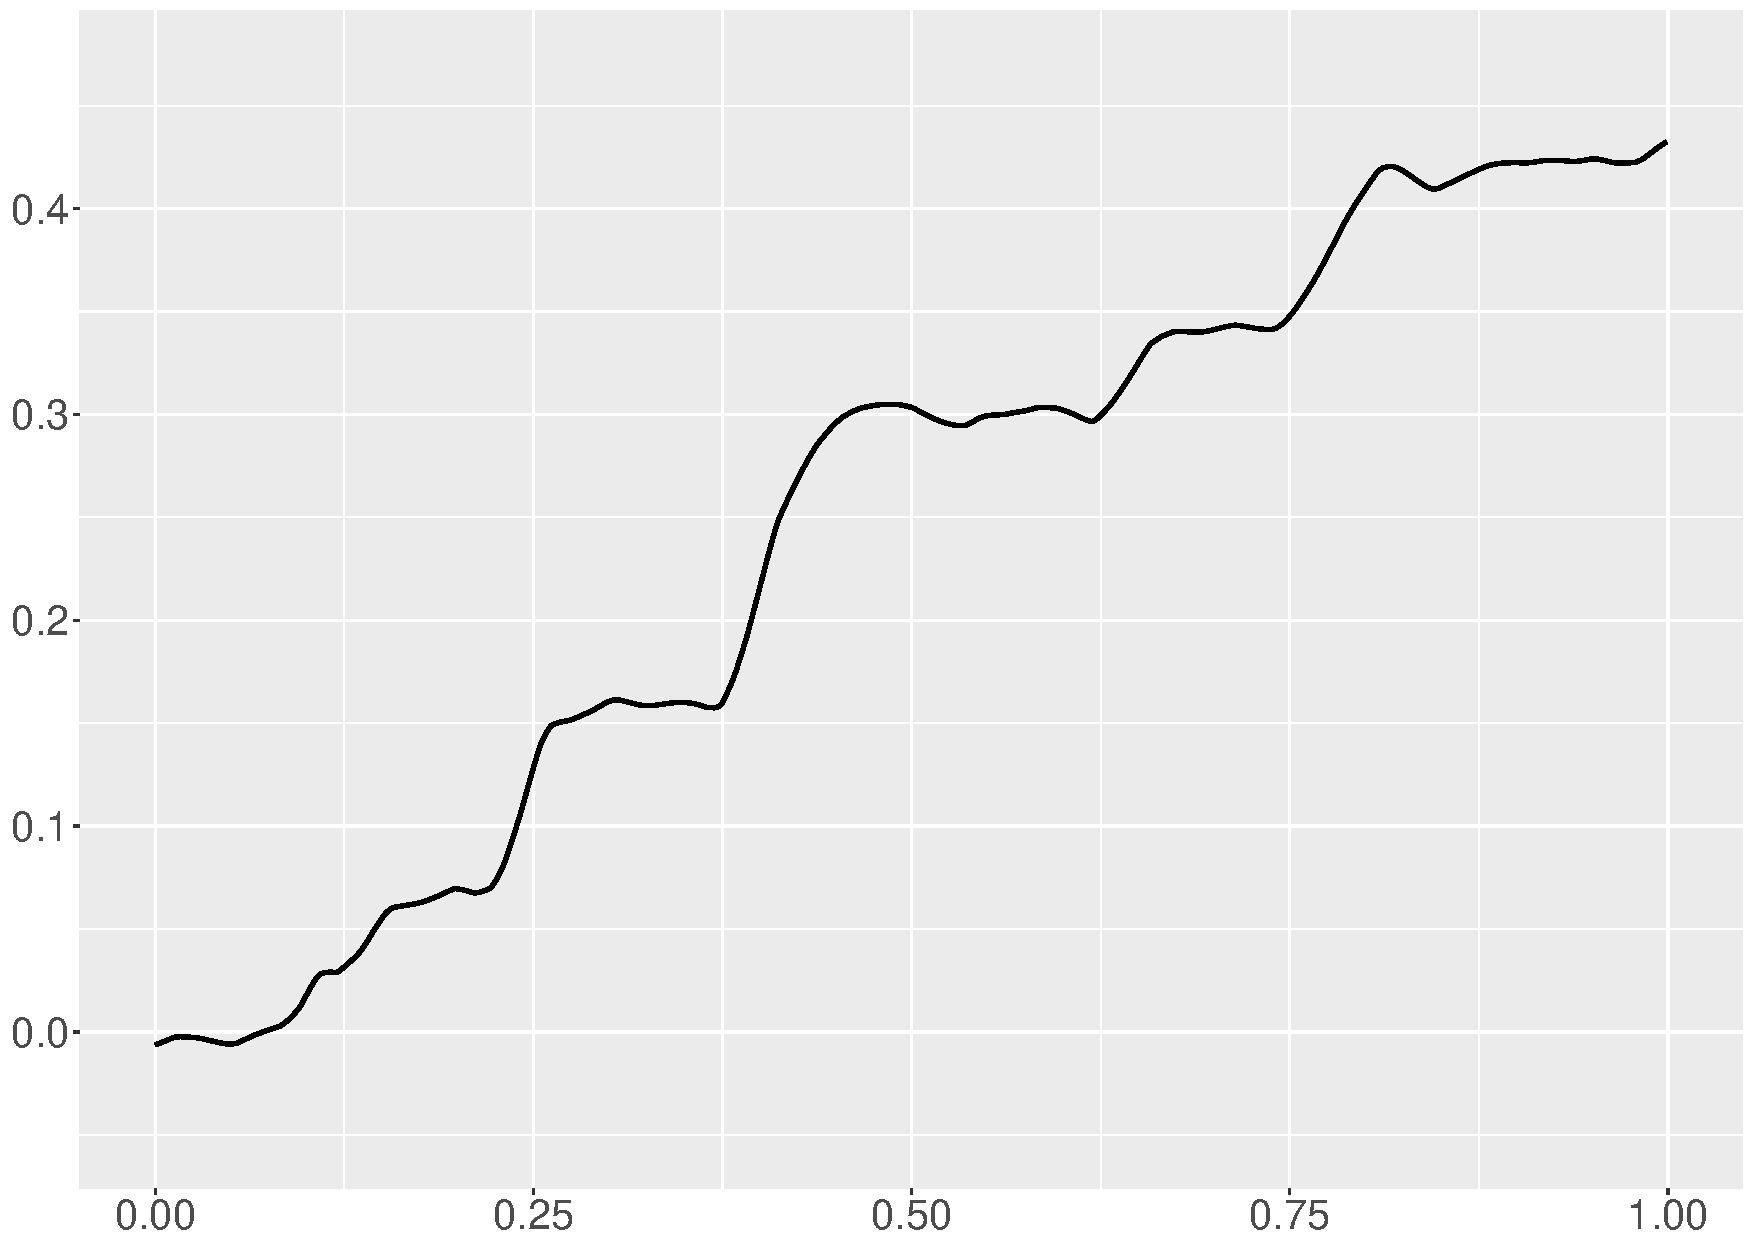
\includegraphics[width=\linewidth,height=0.45\textwidth]{Chapters/02TractorSplineTheory/plot/ggplot/ggBumpsGamma.pdf}
    \caption{Reconstruction by V-spline setting $\gamma=0$}
    \end{subfigure}
  \begin{subfigure}{0.45\textwidth}
    \centering
    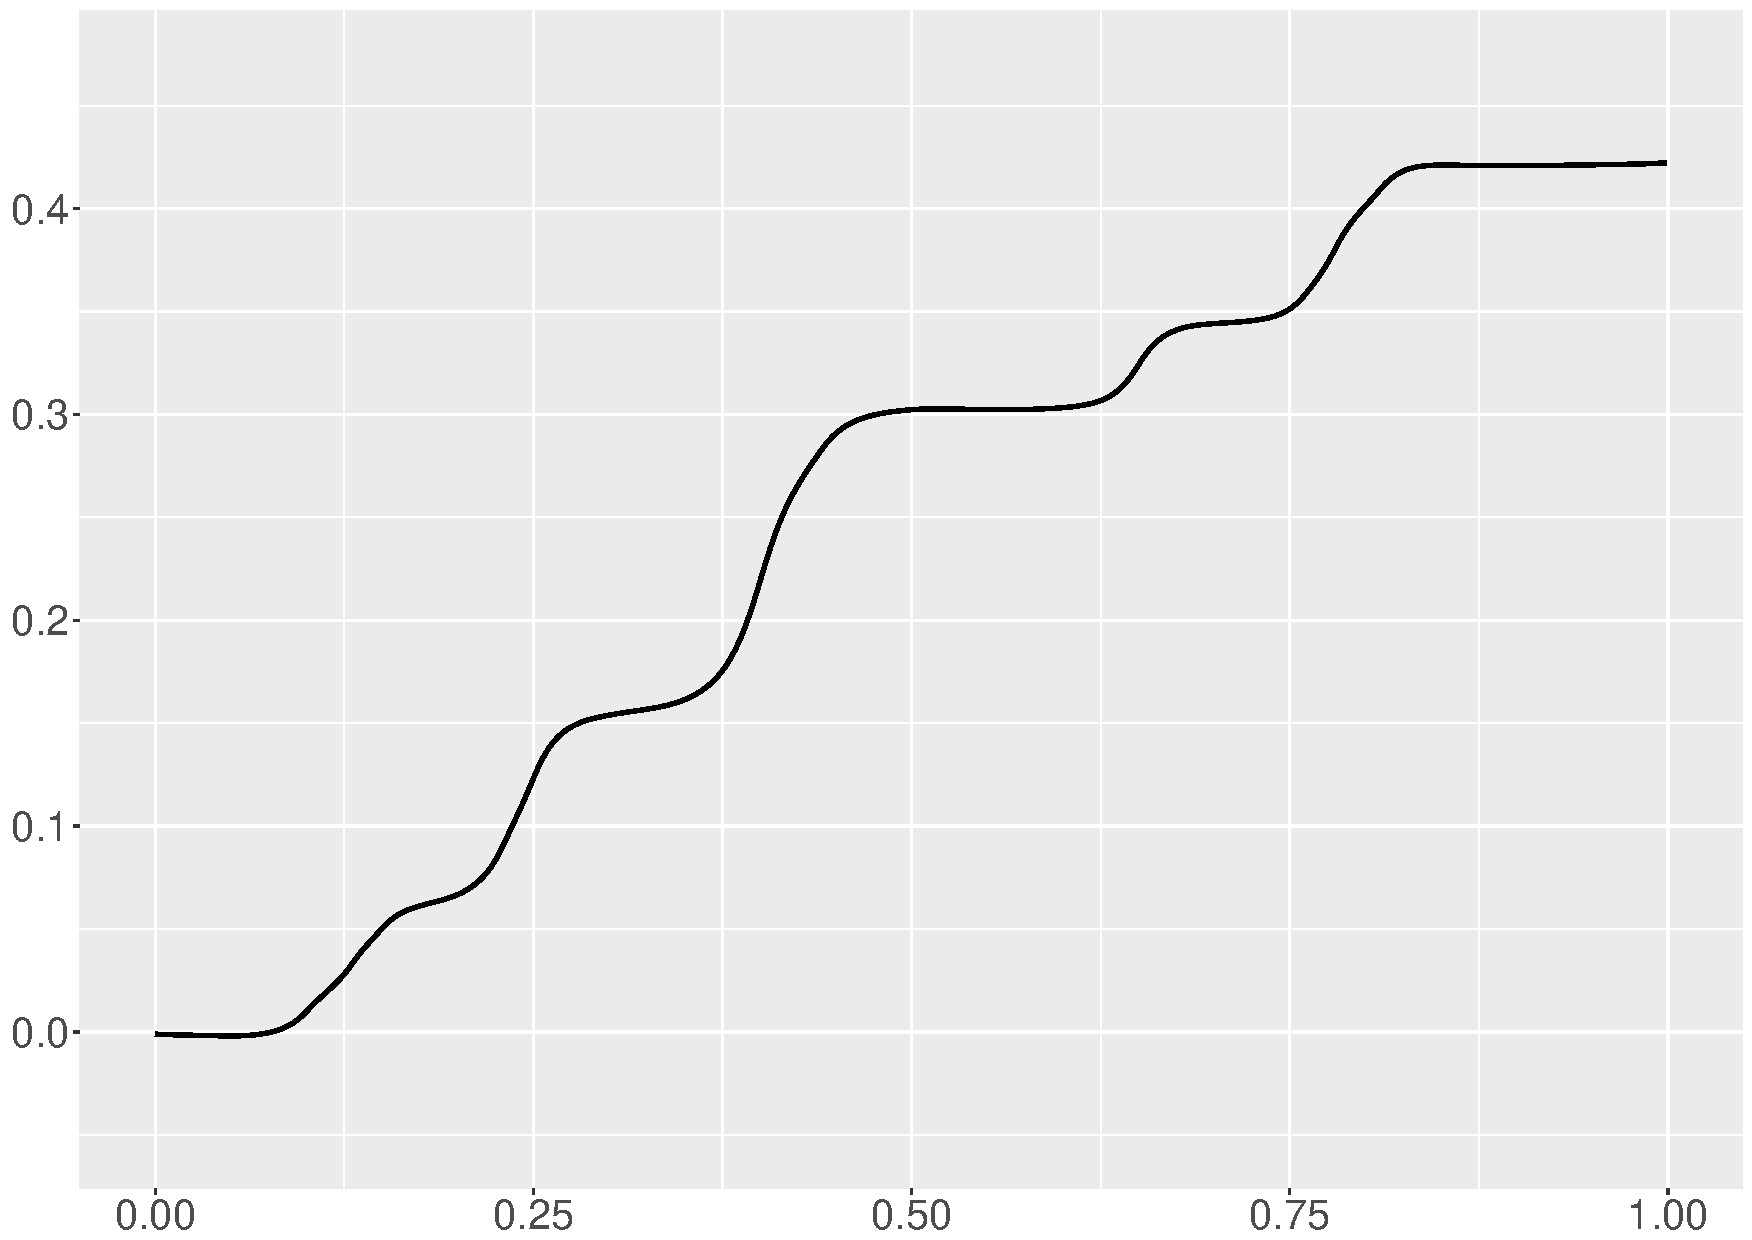
\includegraphics[width=\linewidth,height=0.45\textwidth]{Chapters/02TractorSplineTheory/plot/ggplot/ggBumpsTractorAPT.pdf}
    \caption{Reconstruction by V-spline with conventional penalty term}
    \end{subfigure}
    \begin{subfigure}{0.45\textwidth}
    \centering
    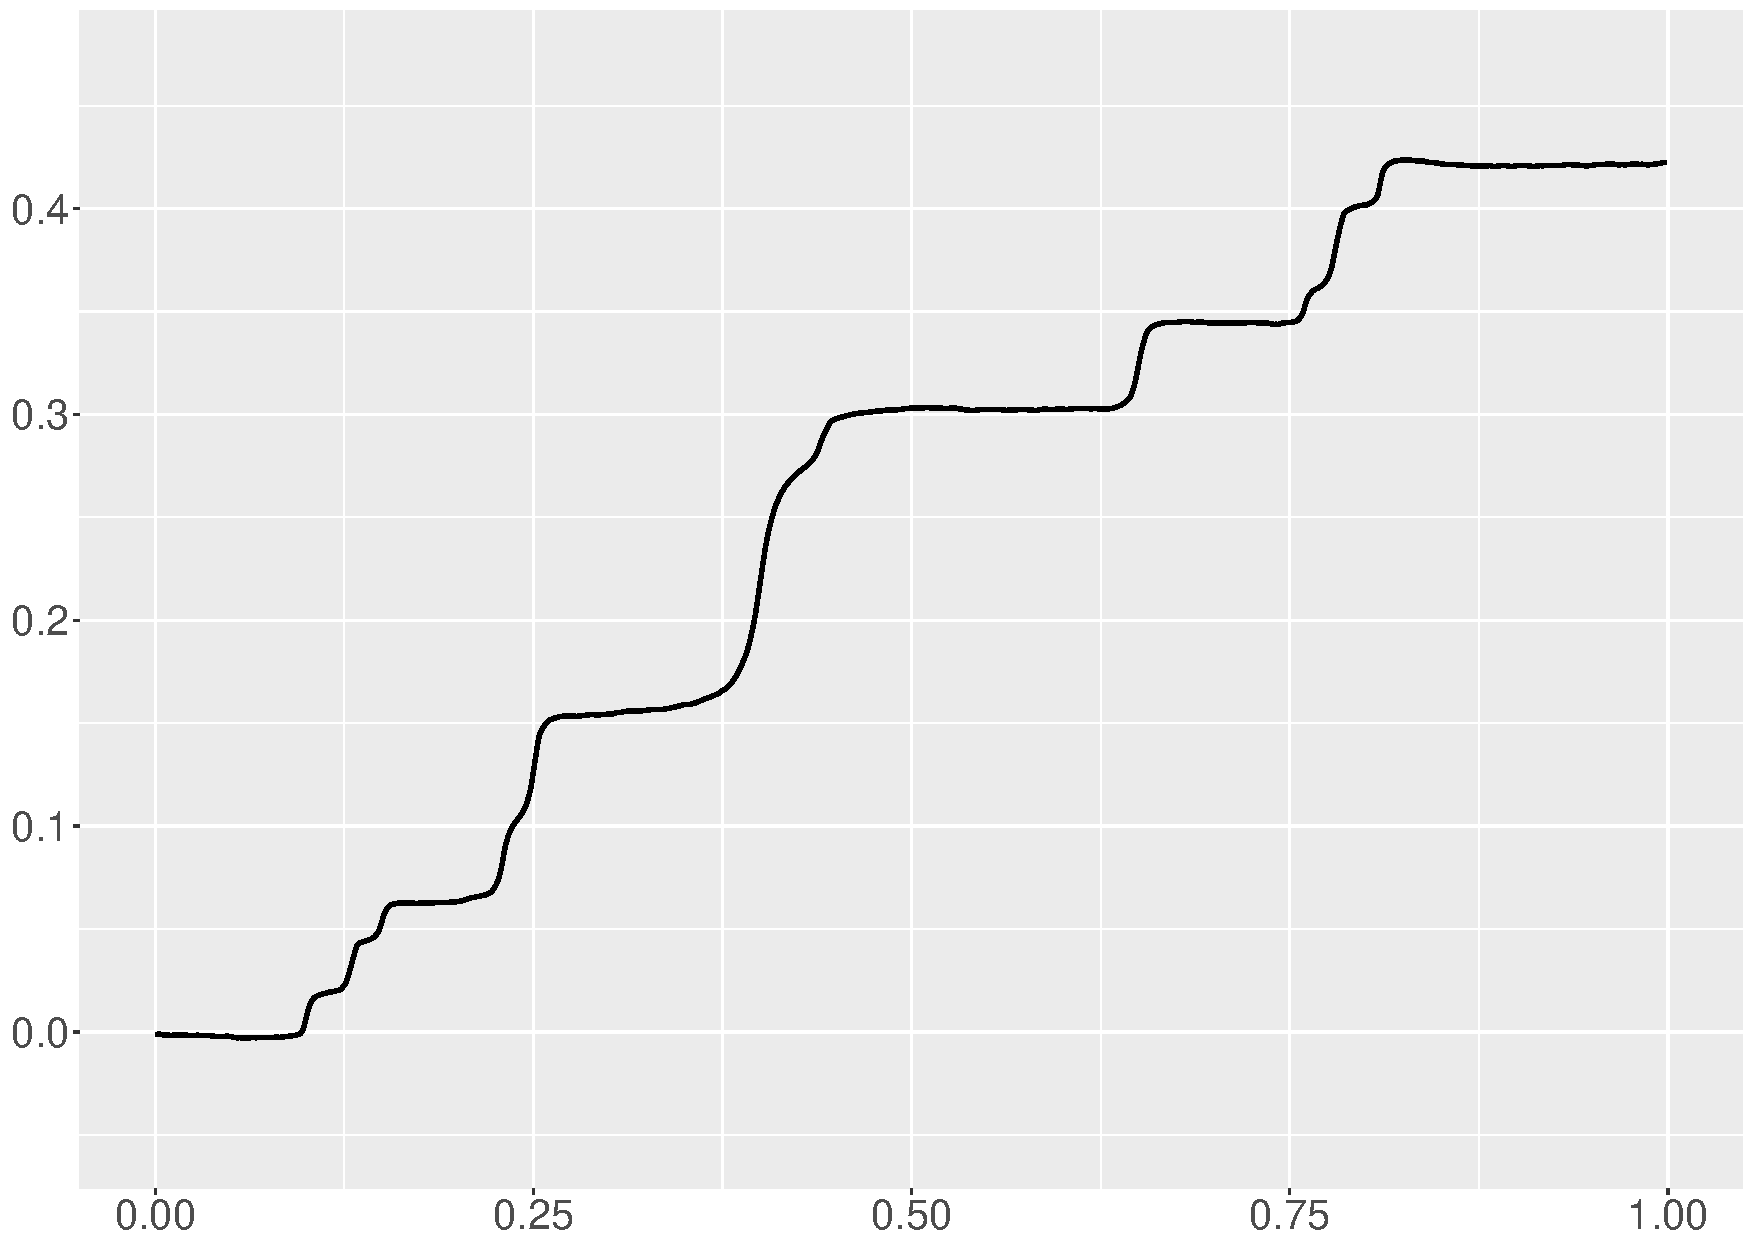
\includegraphics[width=\linewidth,height=0.45\textwidth]{Chapters/02TractorSplineTheory/plot/ggplot/ggBumpsTractor.pdf}
    \caption{Reconstruction by the proposed V-spline}
    \end{subfigure}
\caption{Numerical example: $\textit{Bumps}$. Comparison of different reconstruction methods with simulated data.}\label{num2}
 \end{figure}



%\begin{figure}
%  \centering
%    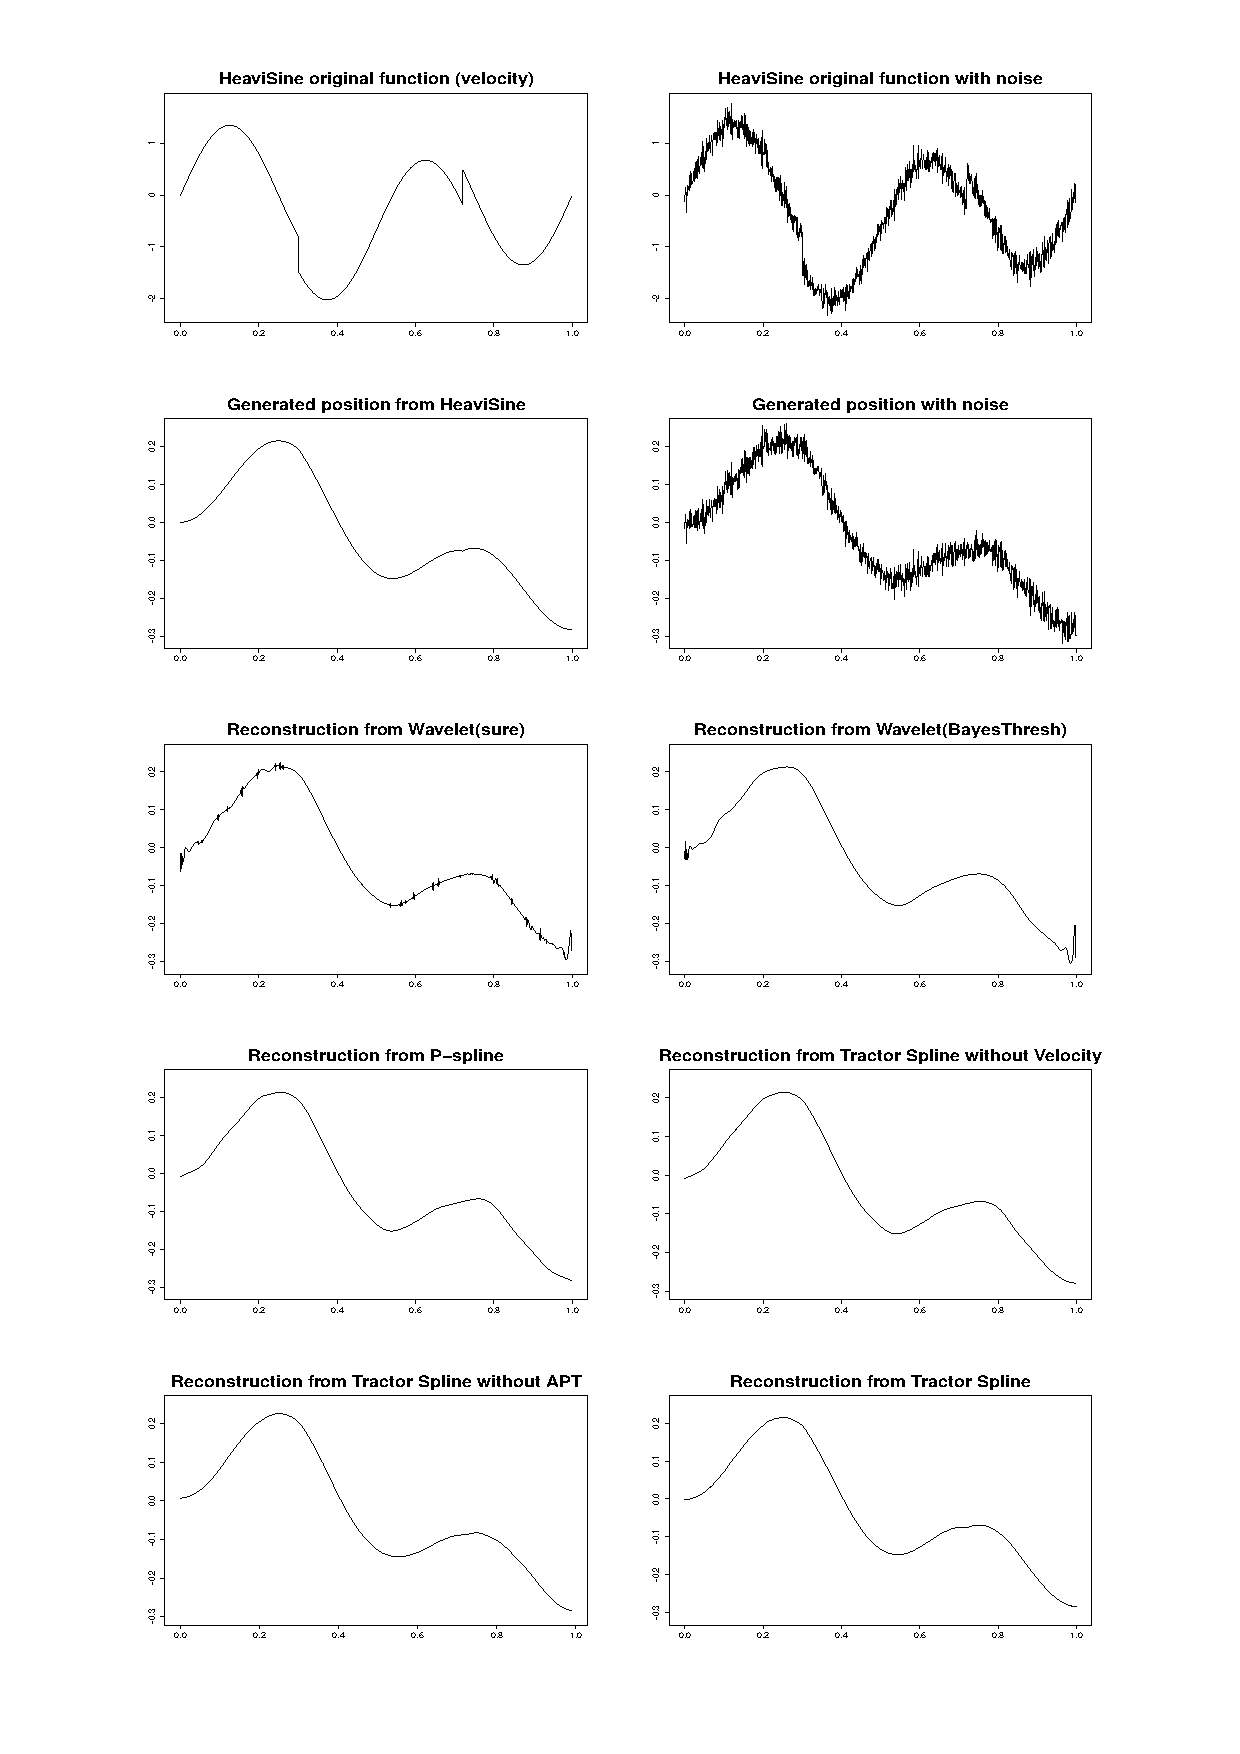
\includegraphics[width=\textwidth,height=14cm]{Chapters/02TractorSplineTheory/plot/heavi10} 
%  \caption{Numerical example: $\textit{HeaviSine}$. (a) The true velocity function. (b) Velocity with Gaussian noise at SNR=7. (c) Generated position function. (d) Position with Gaussian noise at SNR=7. (e) Reconstruction from Wavelet with sure threshold. (f) Reconstruction from Wavelet with BayesThresh approach. (g) Reconstruction by P-spline. (h) Reconstruction by V-spline setting $\gamma=0$. (i) Reconstruction by V-spline with normal penalty term. (j) Reconstruction by proposed V-spline.}\label{num3}
%\end{figure}



\begin{figure}
    \centering
    \begin{subfigure}{0.45\textwidth}
    \centering
    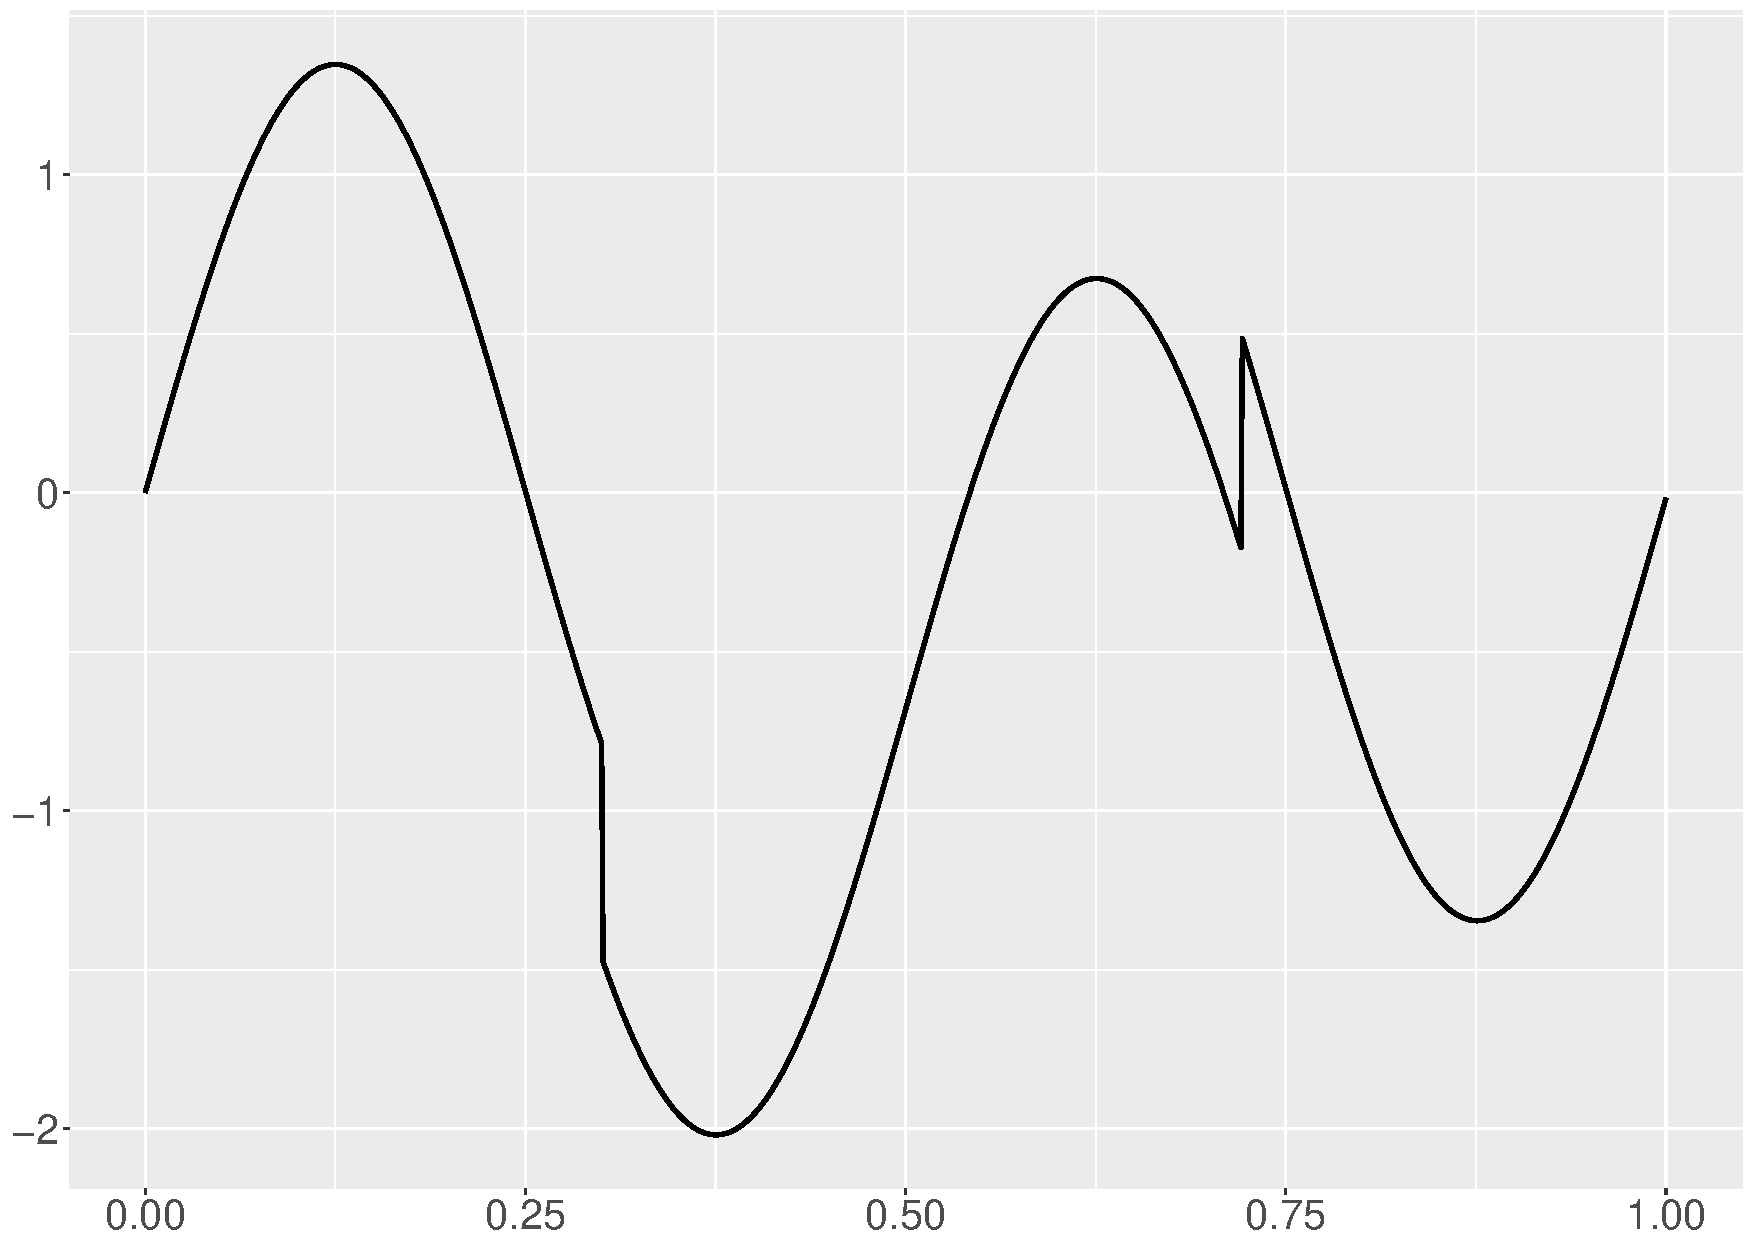
\includegraphics[width=\linewidth,height=0.45\textwidth]{Chapters/02TractorSplineTheory/plot/ggplot/ggHeaviSine.pdf}
    \caption{True \textit{HeaviSine} function}
    \end{subfigure}%
    \begin{subfigure}{0.45\textwidth}
    \centering
    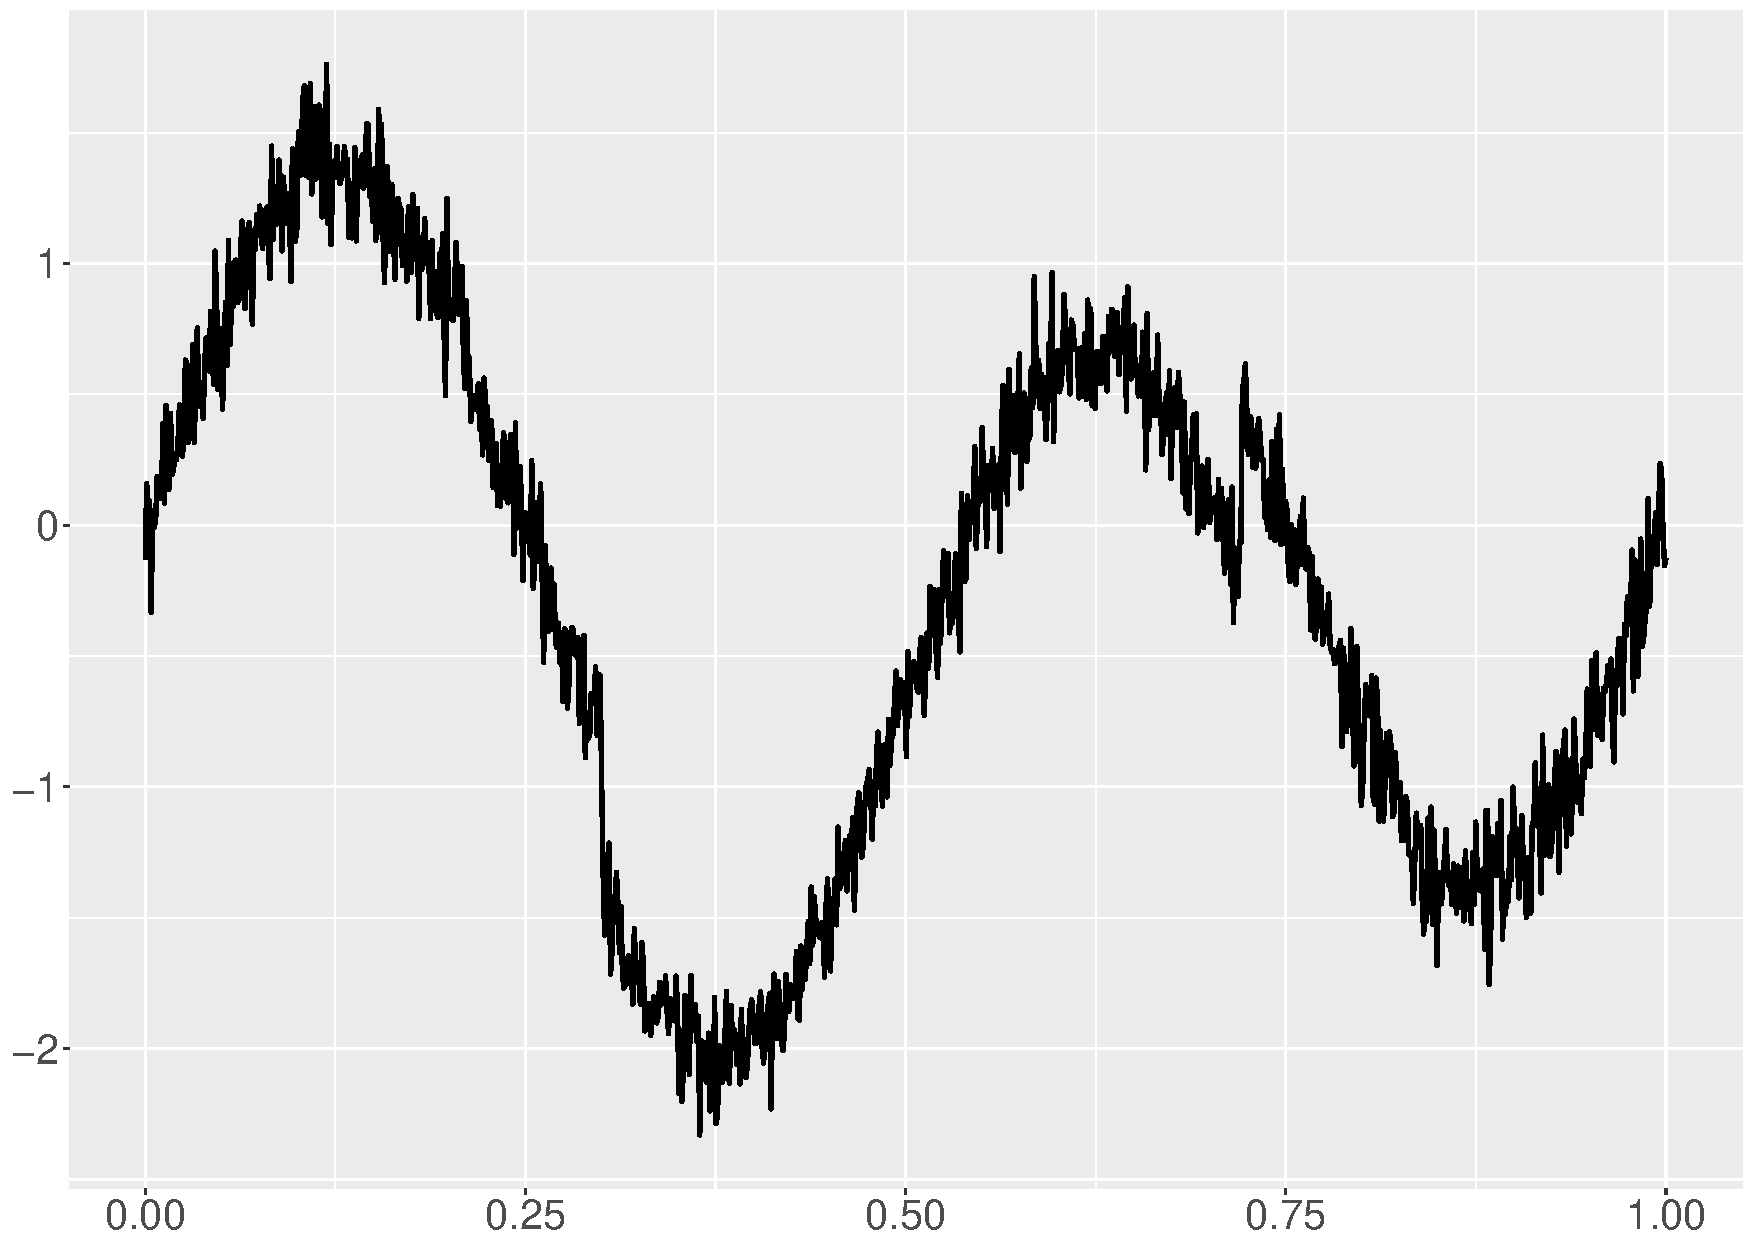
\includegraphics[width=\linewidth,height=0.45\textwidth]{Chapters/02TractorSplineTheory/plot/ggplot/ggHeaviSineNoise.pdf}
    \caption{Noisy \textit{HeaviSine} at \textit{SNR}=7}
    \end{subfigure}
    \begin{subfigure}{0.45\textwidth}
    \centering
    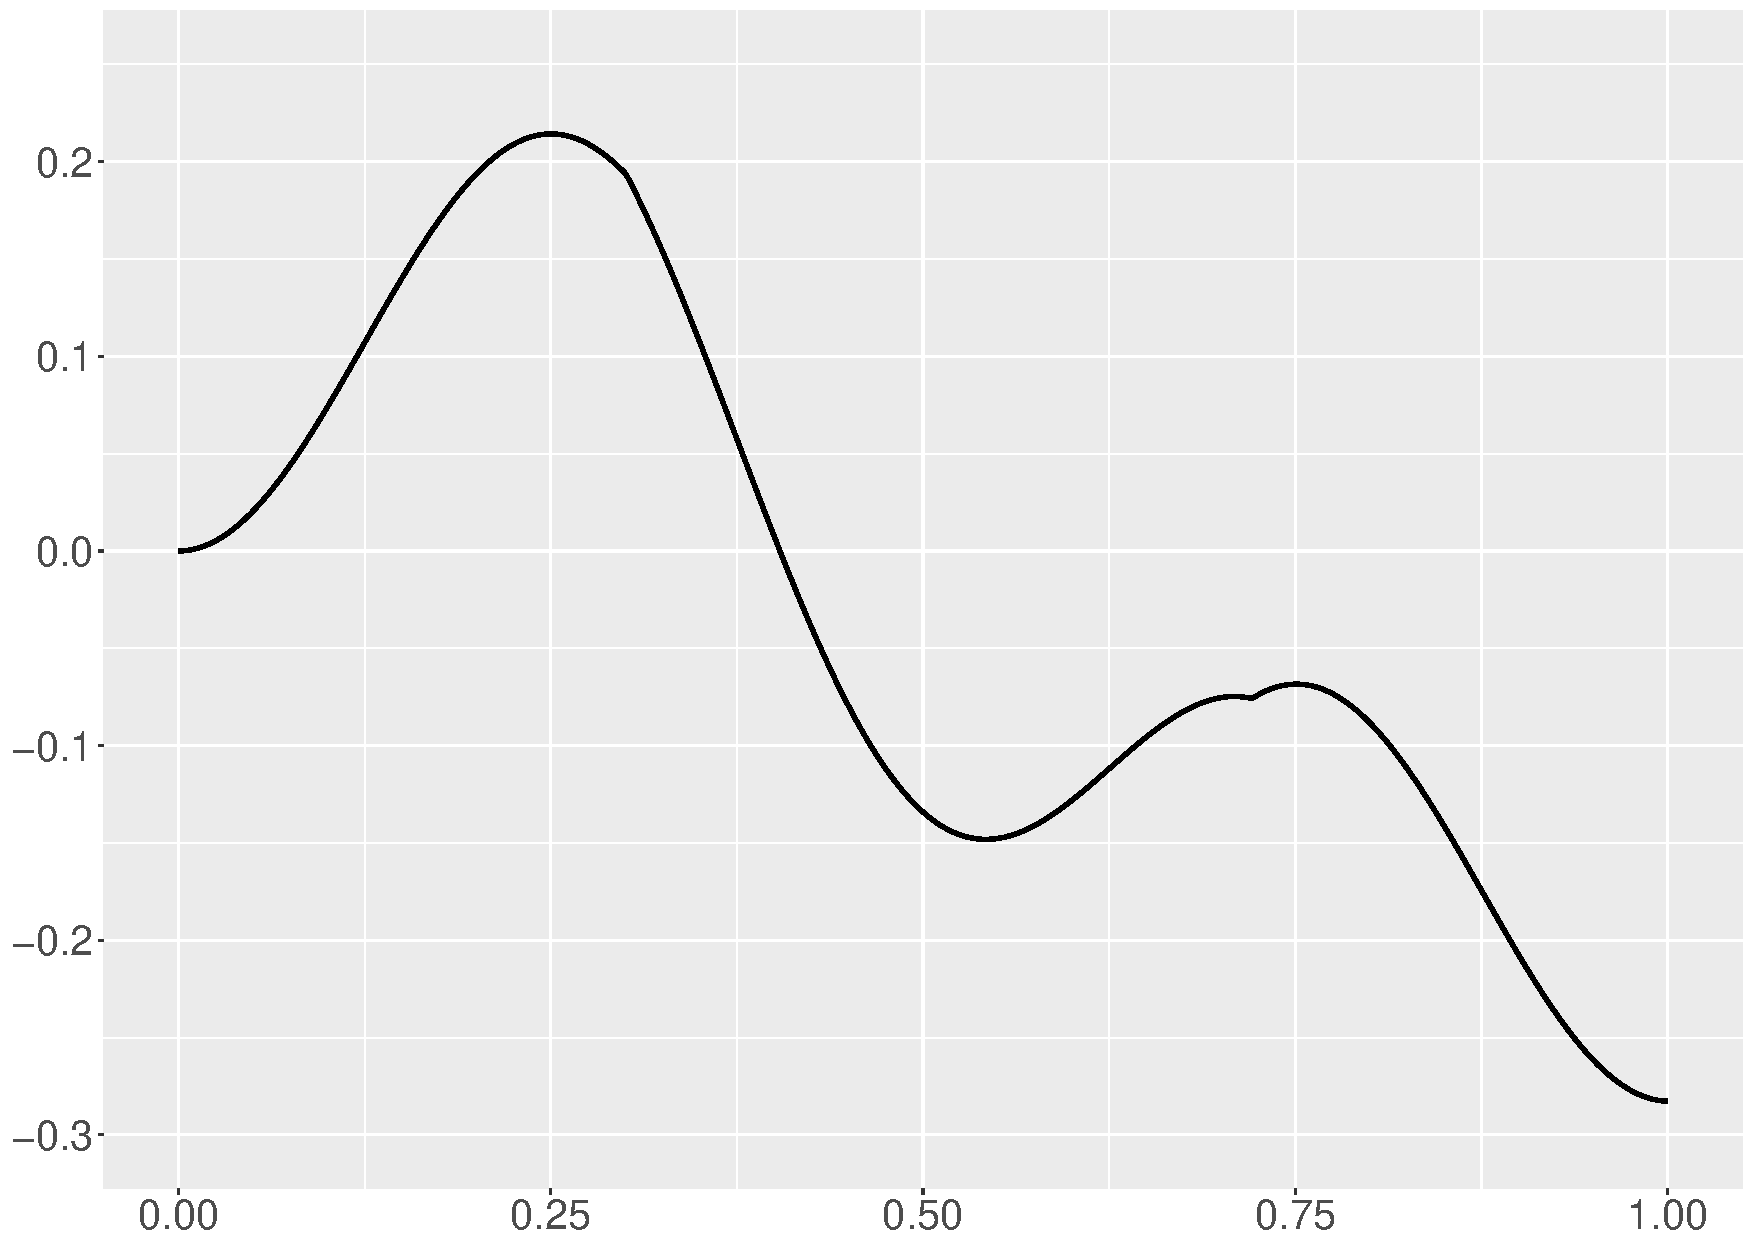
\includegraphics[width=\linewidth,height=0.45\textwidth]{Chapters/02TractorSplineTheory/plot/ggplot/ggHeaviSinePosition.pdf}
    \caption{Generated positions}
    \end{subfigure}
    \begin{subfigure}{0.45\textwidth}
    \centering
    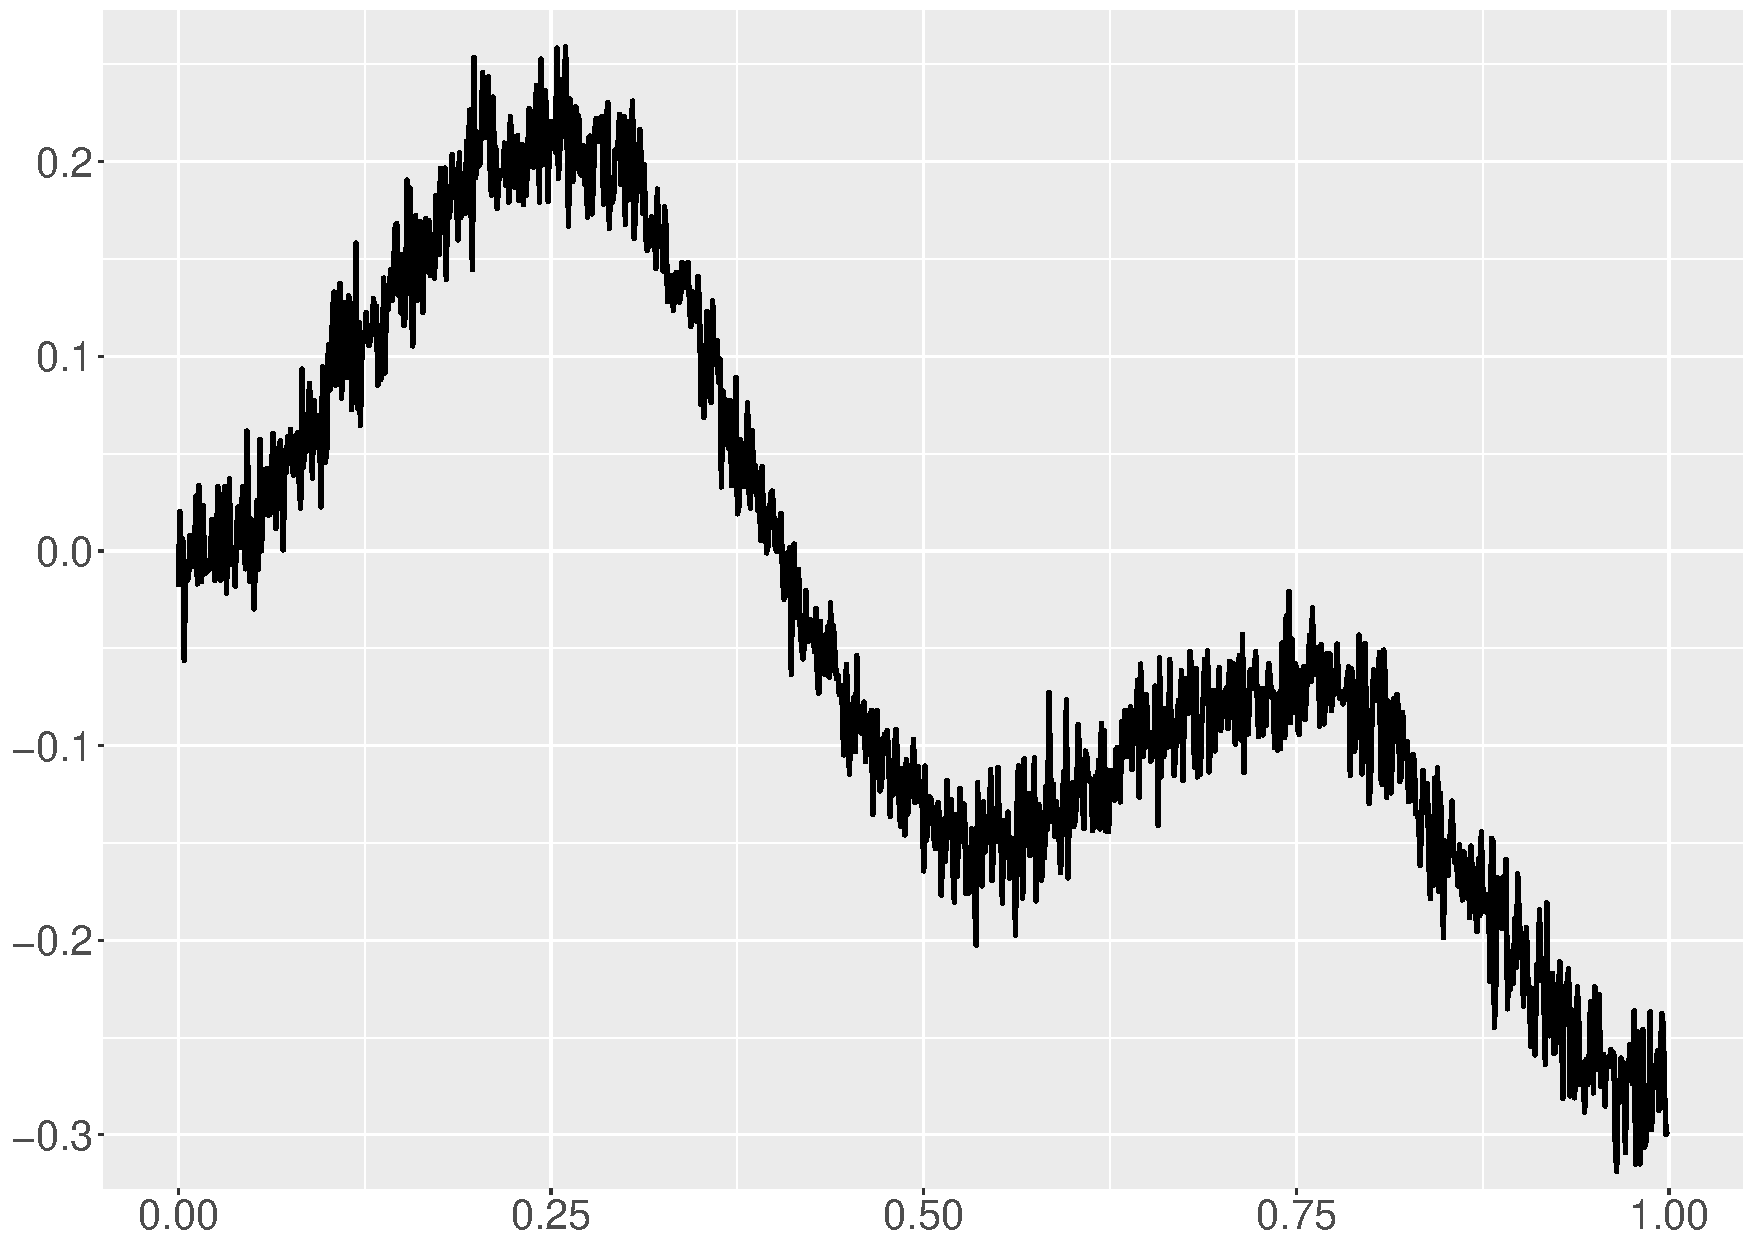
\includegraphics[width=\linewidth,height=0.45\textwidth]{Chapters/02TractorSplineTheory/plot/ggplot/ggHeaviSinePositionNoise.pdf}
    \caption{Noisy position at \textit{SNR}=7}
    \end{subfigure}
    \begin{subfigure}{0.45\textwidth}
    \centering
    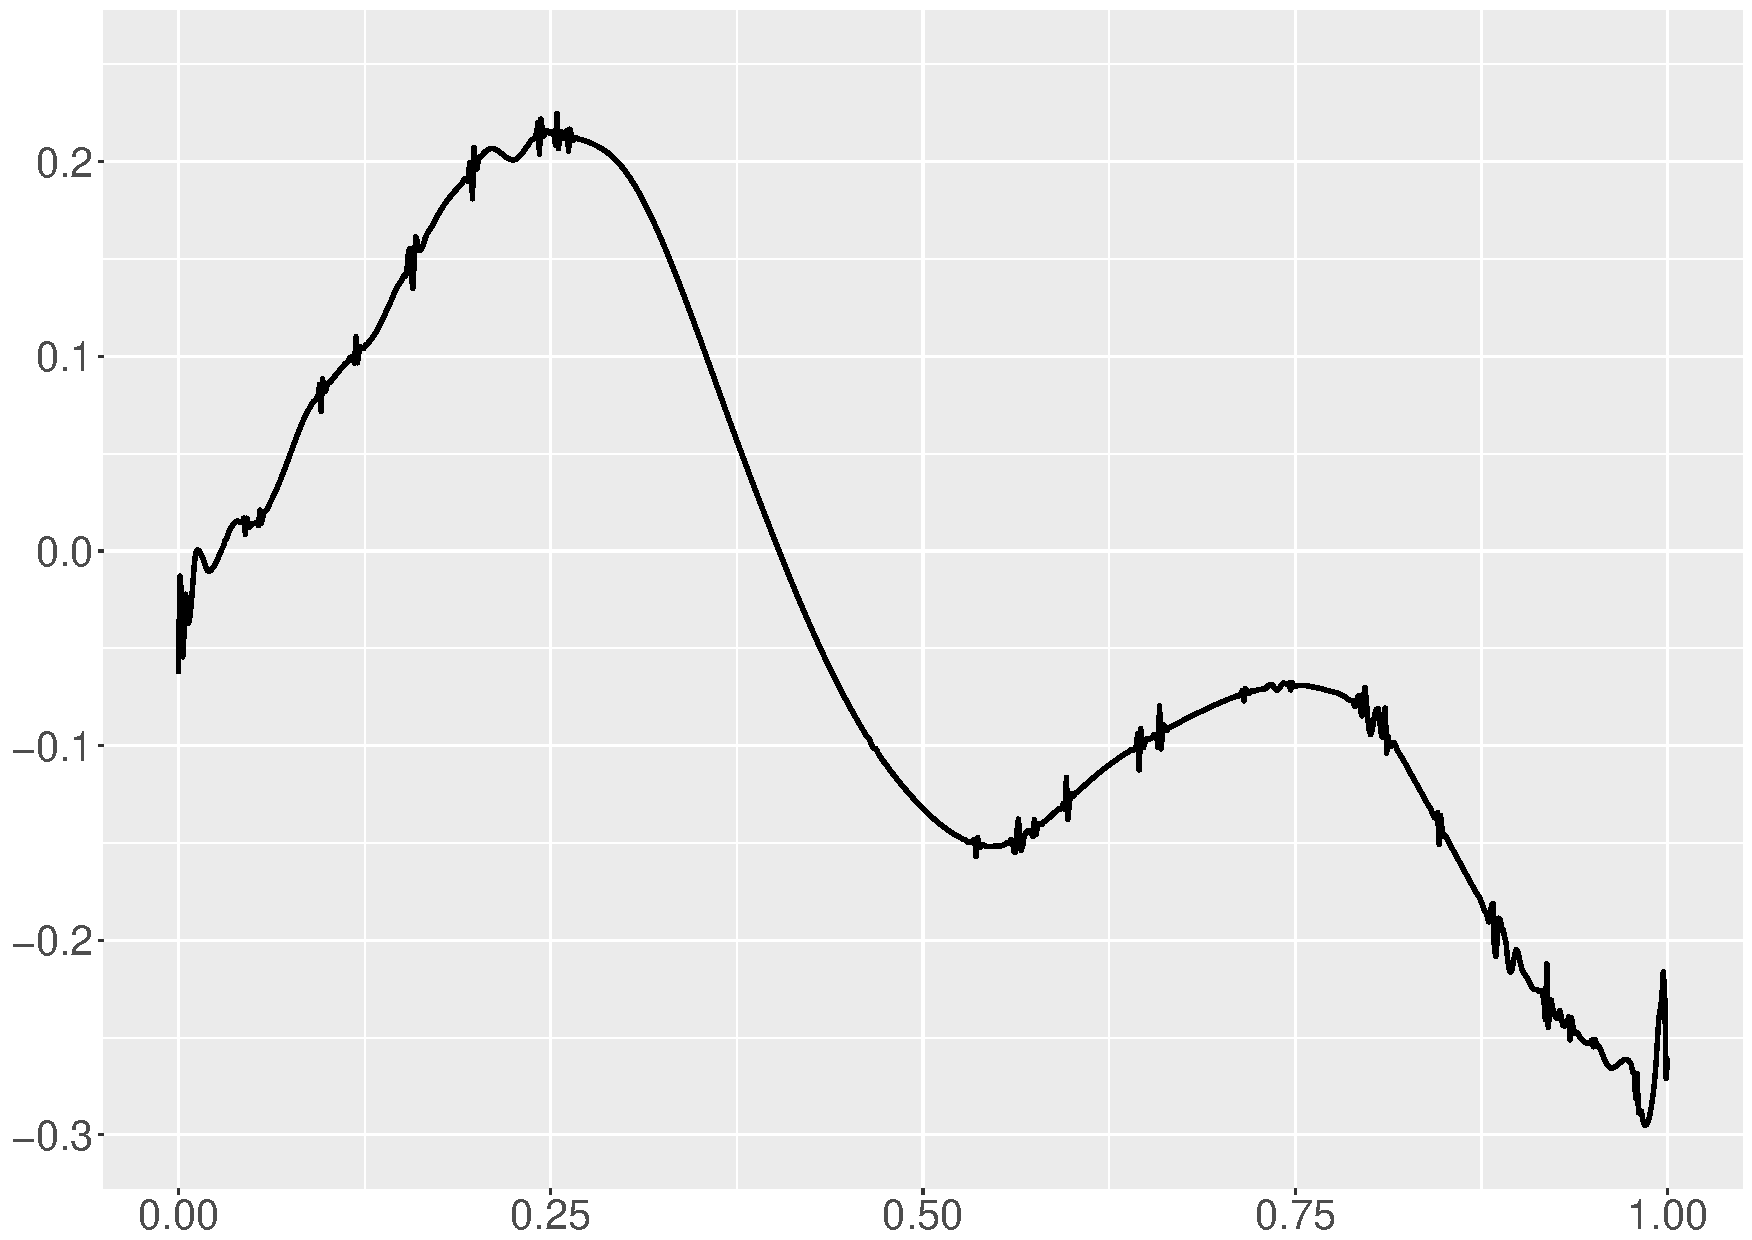
\includegraphics[width=\linewidth,height=0.45\textwidth]{Chapters/02TractorSplineTheory/plot/ggplot/ggHeaviSineSure.pdf}
    \caption{Reconstruction from Wavelet by sure threshold}
    \end{subfigure}
    \begin{subfigure}{0.45\textwidth}
    \centering
    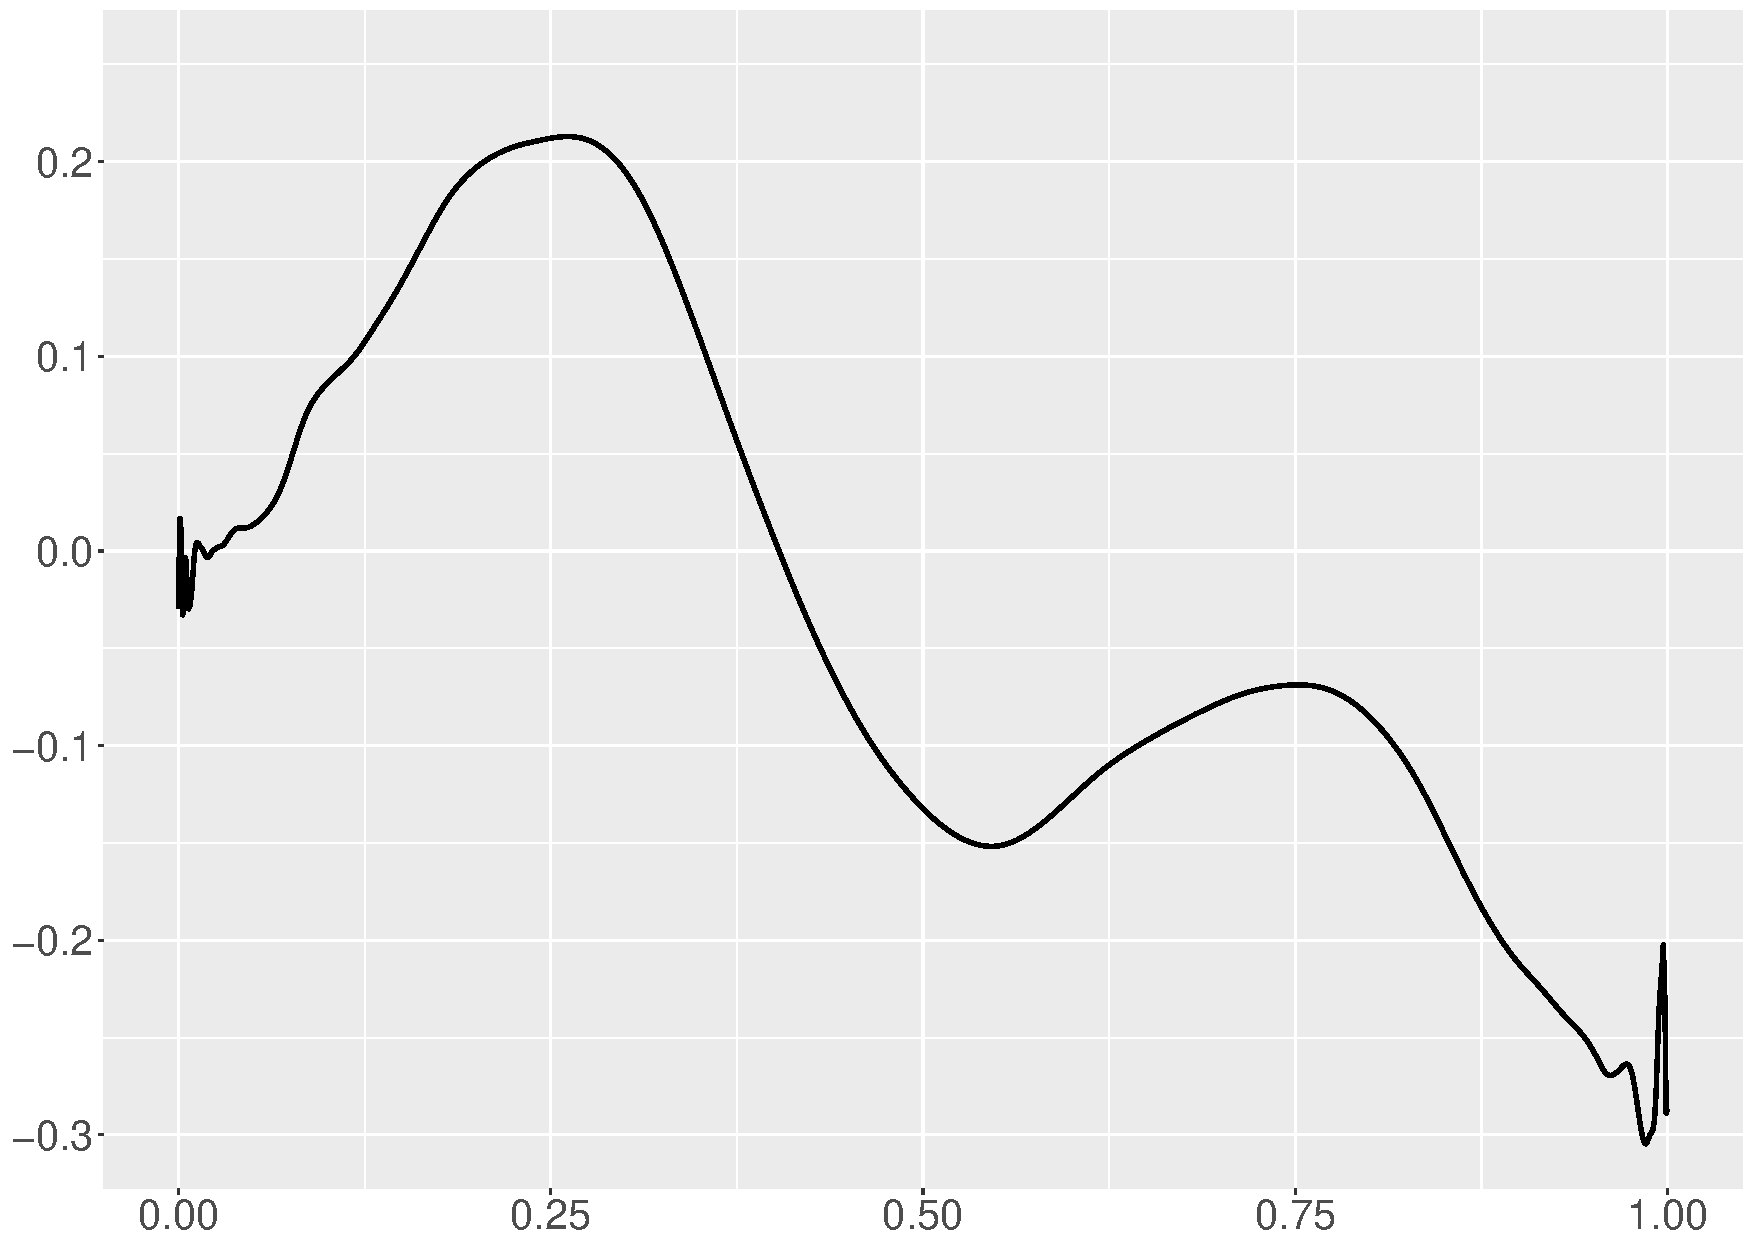
\includegraphics[width=\linewidth,height=0.45\textwidth]{Chapters/02TractorSplineTheory/plot/ggplot/ggHeaviSineBayes.pdf}
    \caption{Reconstruction from Wavelet by BayesThresh approach}
    \end{subfigure}
    \begin{subfigure}{0.45\textwidth}
    \centering
    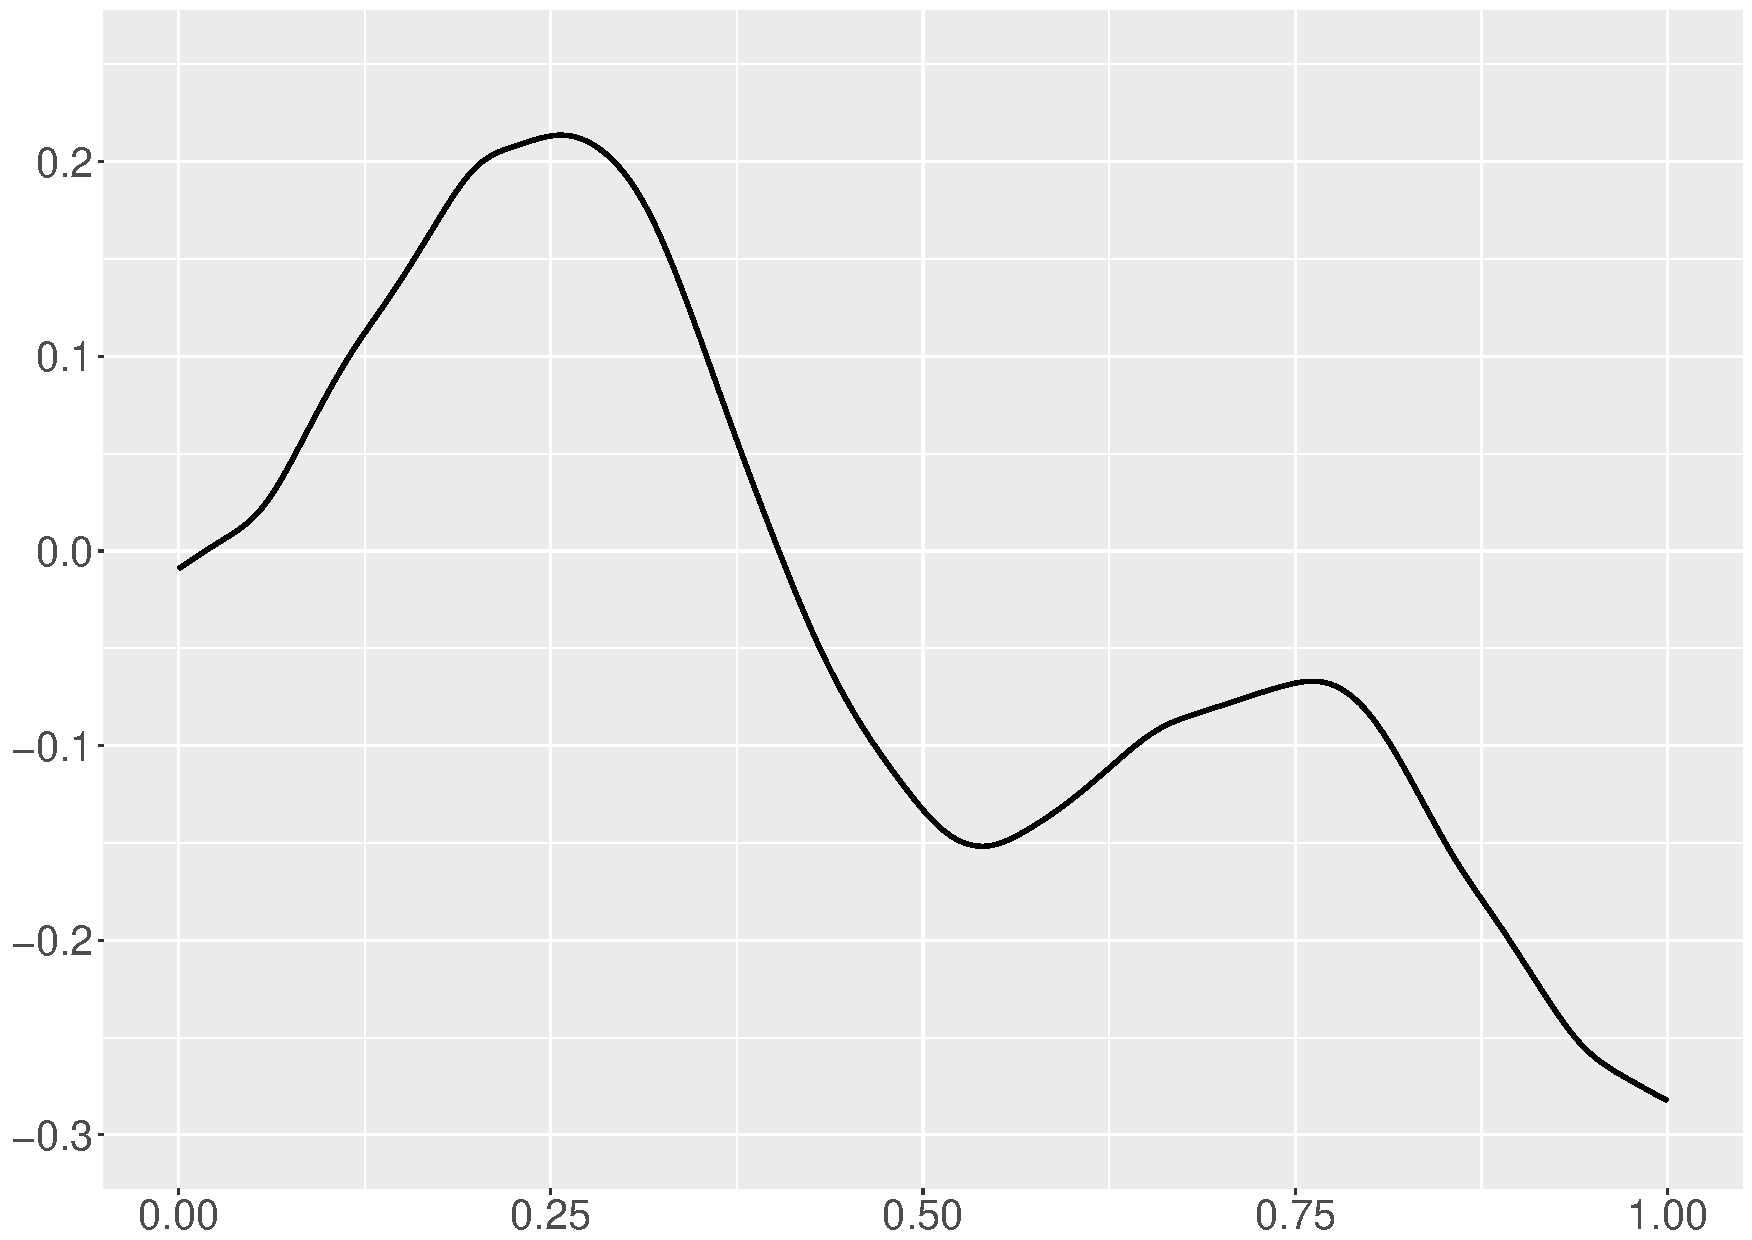
\includegraphics[width=\linewidth,height=0.45\textwidth]{Chapters/02TractorSplineTheory/plot/ggplot/ggHeaviSinePSpline.pdf}
    \caption{Reconstruction by P-spline \\\mbox{  } }
    \end{subfigure}
    \begin{subfigure}{0.45\textwidth}
    \centering
    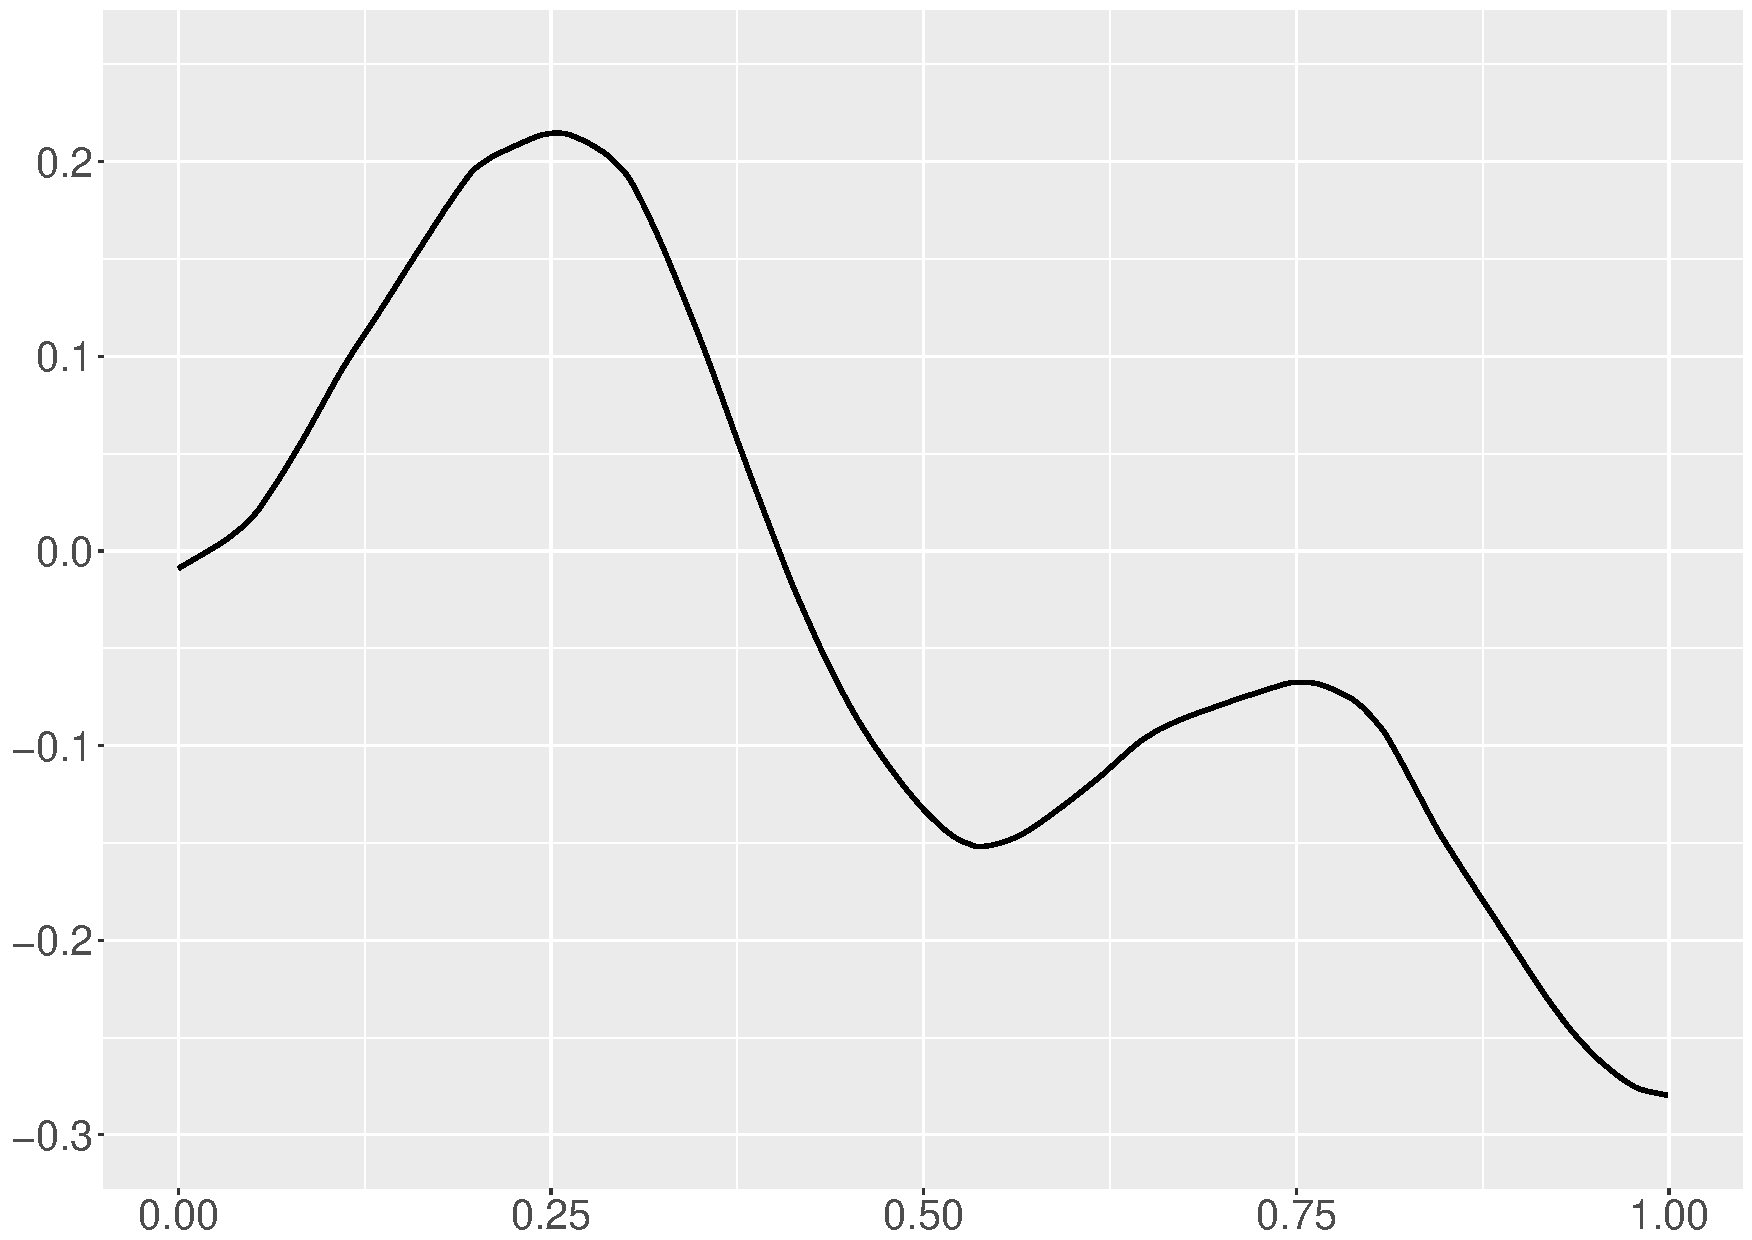
\includegraphics[width=\linewidth,height=0.45\textwidth]{Chapters/02TractorSplineTheory/plot/ggplot/ggHeaviSineGamma.pdf}
    \caption{Reconstruction by V-spline setting $\gamma=0$}
    \end{subfigure}
  \begin{subfigure}{0.45\textwidth}
    \centering
    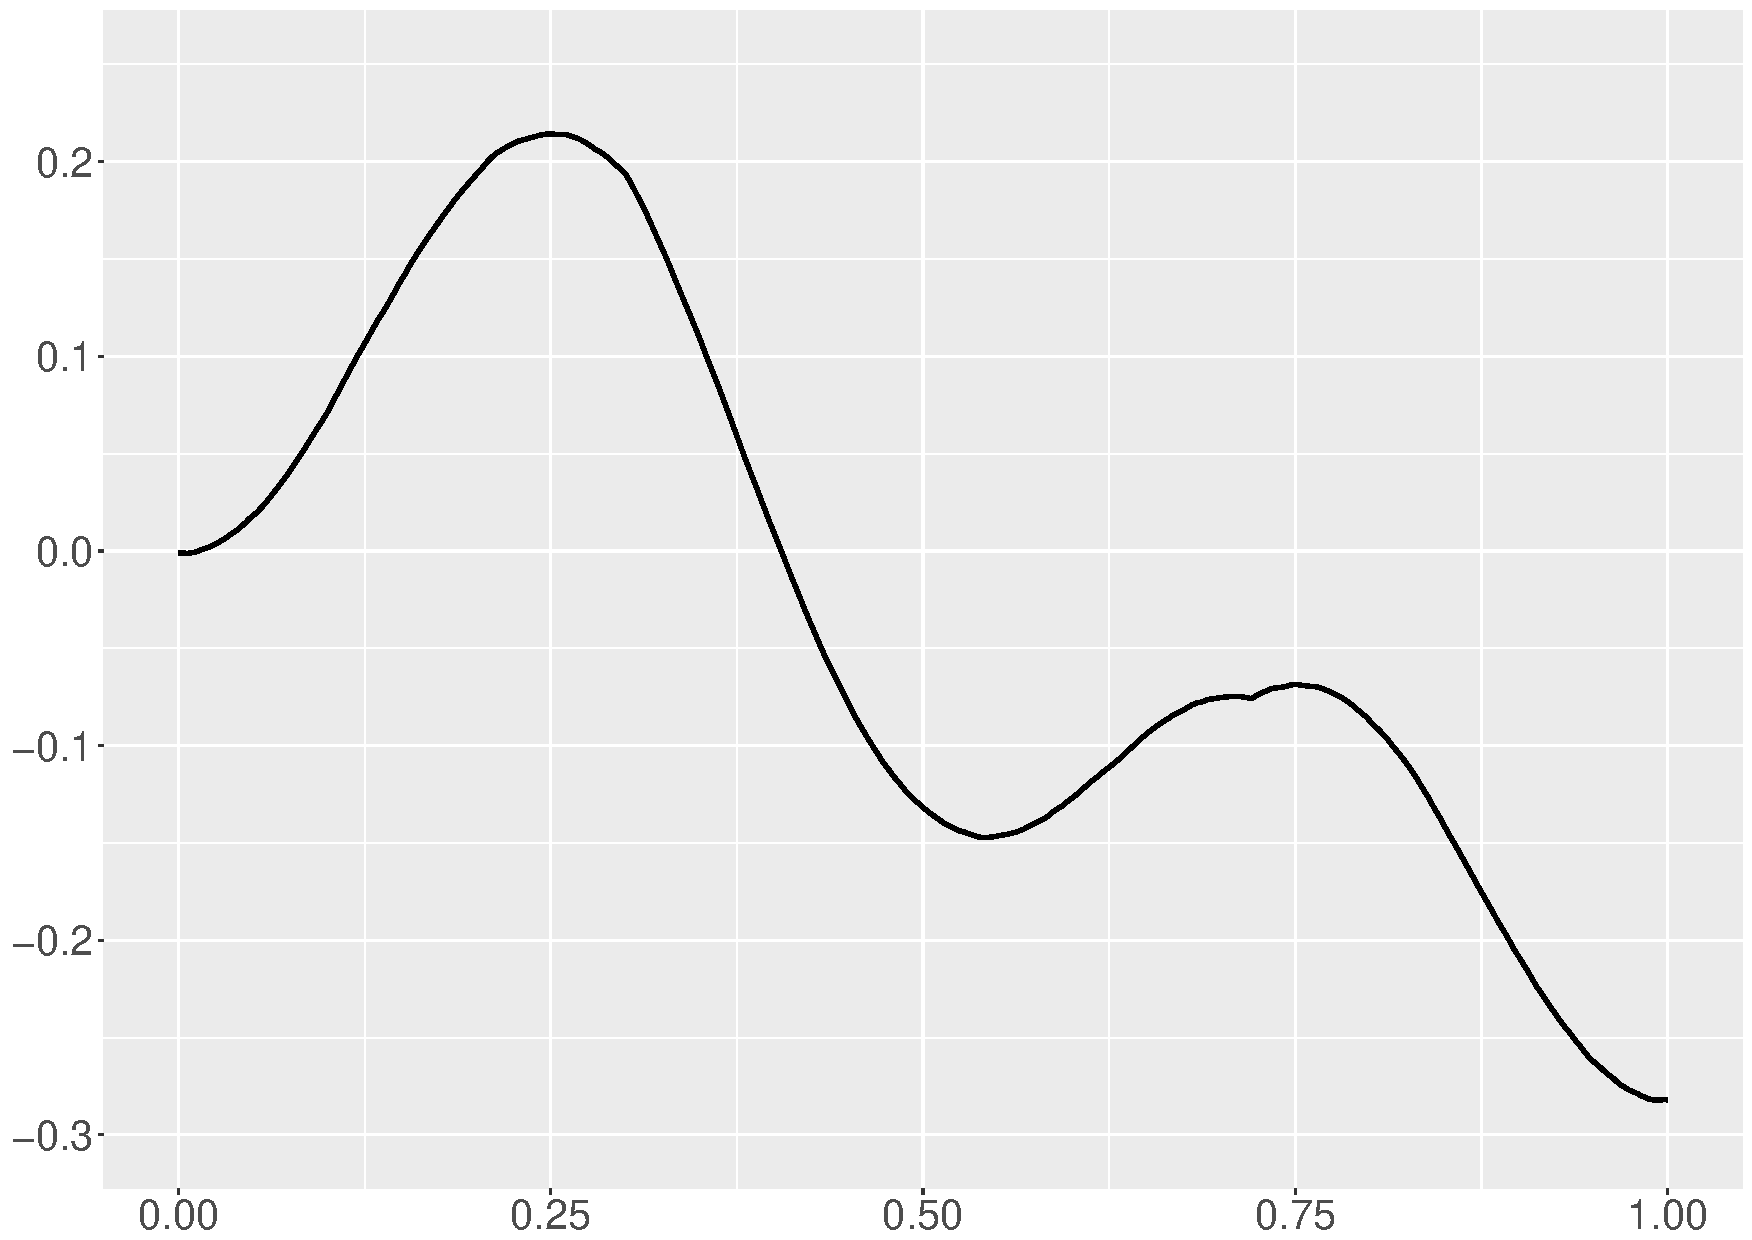
\includegraphics[width=\linewidth,height=0.45\textwidth]{Chapters/02TractorSplineTheory/plot/ggplot/ggHeaviSineTractorAPT.pdf}
    \caption{Reconstruction by V-spline with conventional penalty term}
    \end{subfigure}
    \begin{subfigure}{0.45\textwidth}
    \centering
    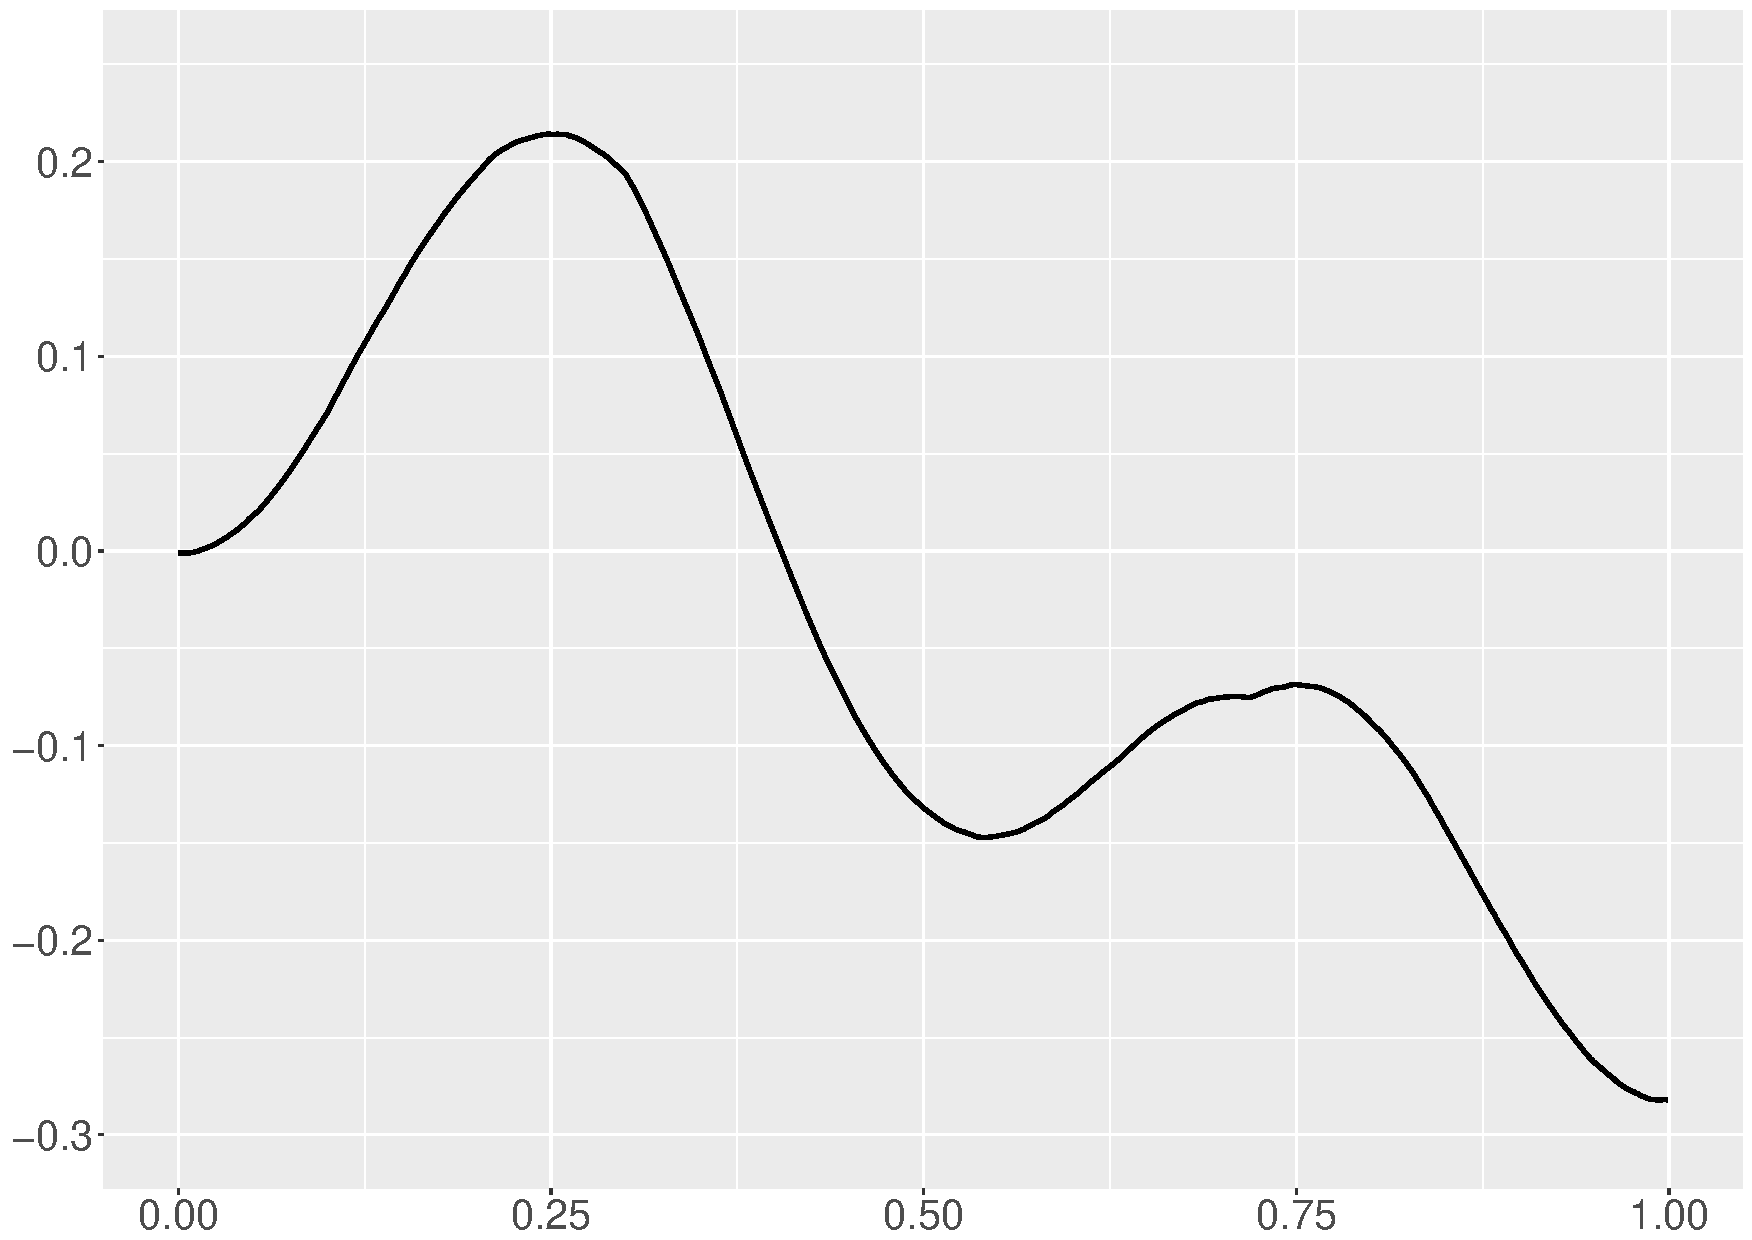
\includegraphics[width=\linewidth,height=0.45\textwidth]{Chapters/02TractorSplineTheory/plot/ggplot/ggHeaviSineTractor.pdf}
    \caption{Reconstruction by the proposed V-spline}
    \end{subfigure}
\caption{Numerical example: $\textit{HeaviSine}$. Comparison of different reconstruction methods with simulated data.}\label{num3}
 \end{figure}

%
%
%\begin{figure}
%  \centering
%         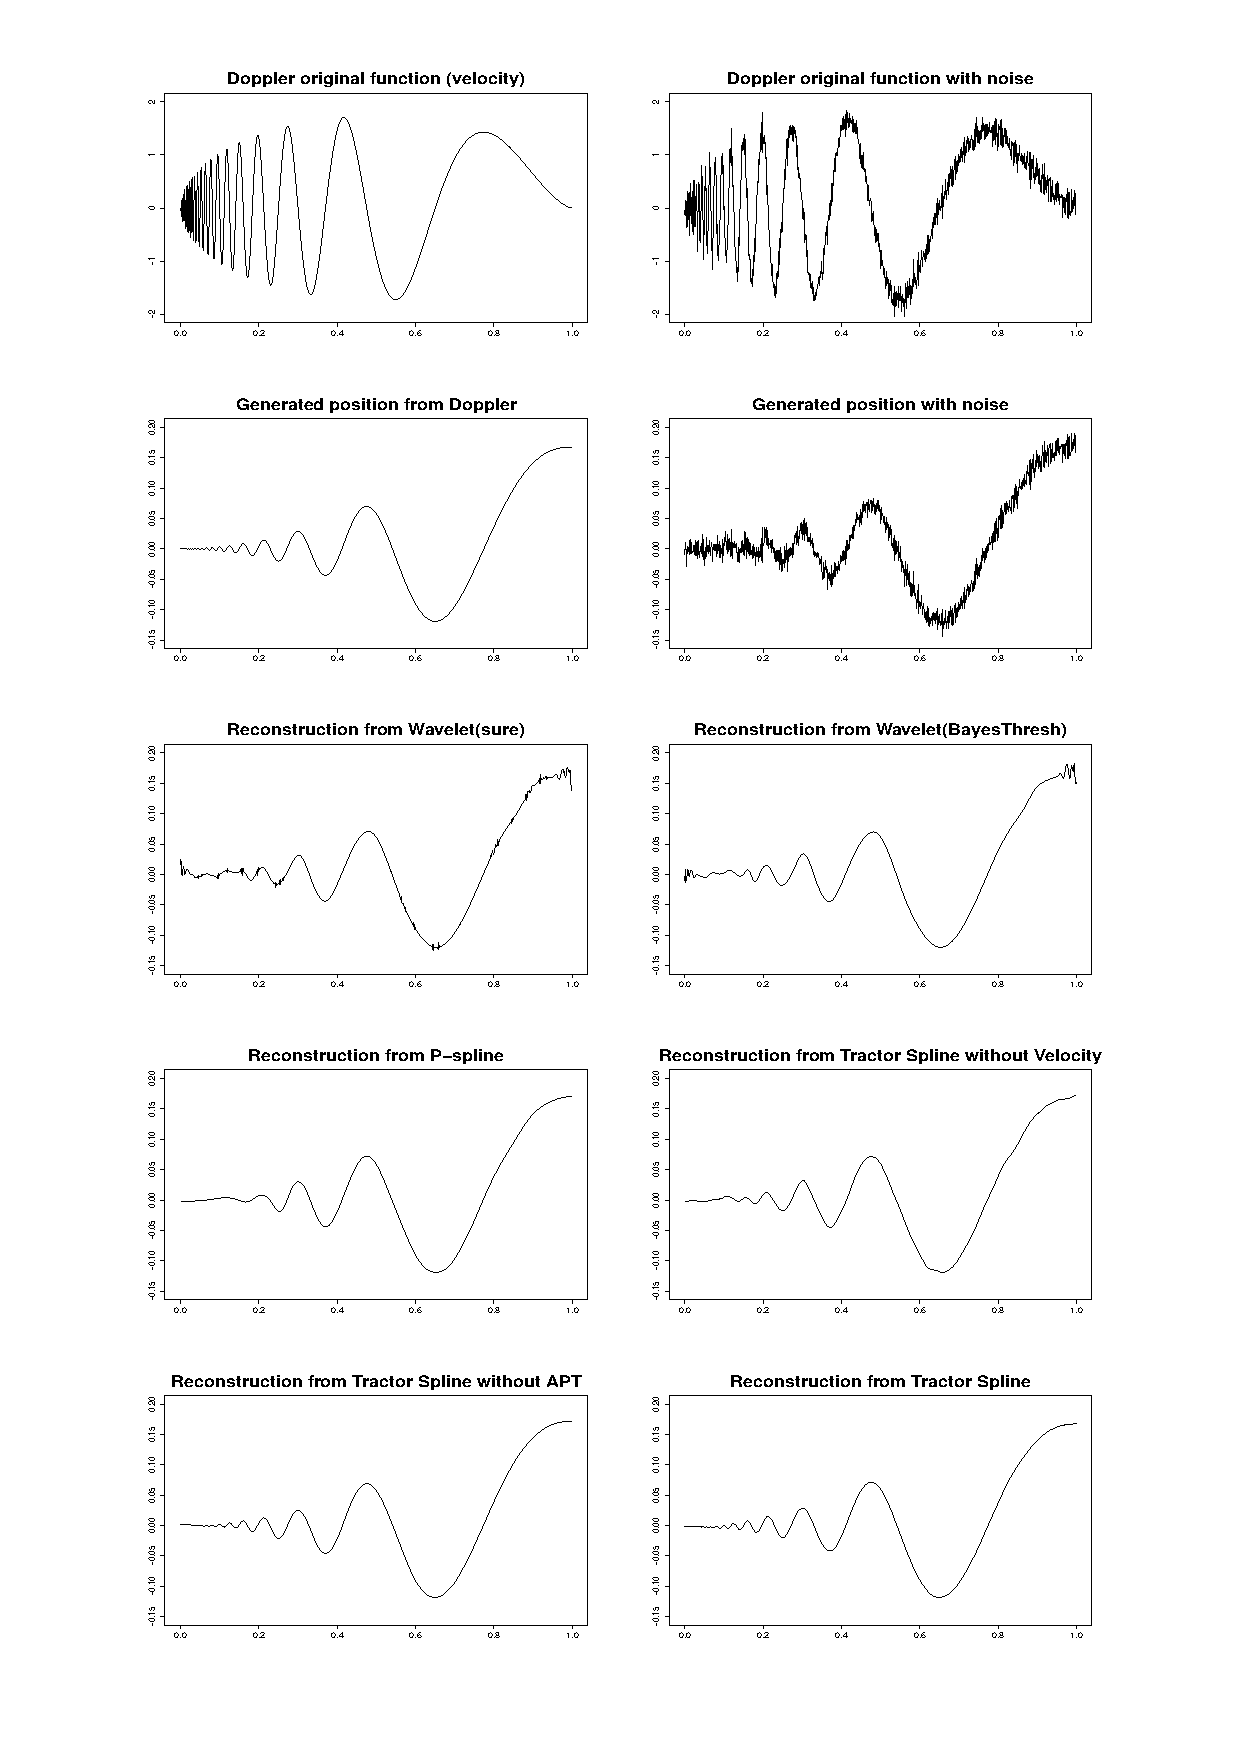
\includegraphics[width=\textwidth,height=14cm]{Chapters/02TractorSplineTheory/plot/doppler10} 
%  \caption{Numerical example: $\textit{Doppler}$. (a) The true velocity function. (b) Velocity with Gaussian noise at SNR=7. (c) Generated position function. (d) Position with Gaussian noise at SNR=7. (e) Reconstruction from Wavelet with sure threshold. (f) Reconstruction from Wavelet with BayesThresh approach. (g) Reconstruction by P-spline. (h) Reconstruction by V-spline setting $\gamma=0$. (i) Reconstruction by V-spline with normal penalty term. (j) Reconstruction by proposed V-spline.}\label{num4}
%\end{figure}


\begin{figure}
    \centering
    \begin{subfigure}{0.45\textwidth}
    \centering
    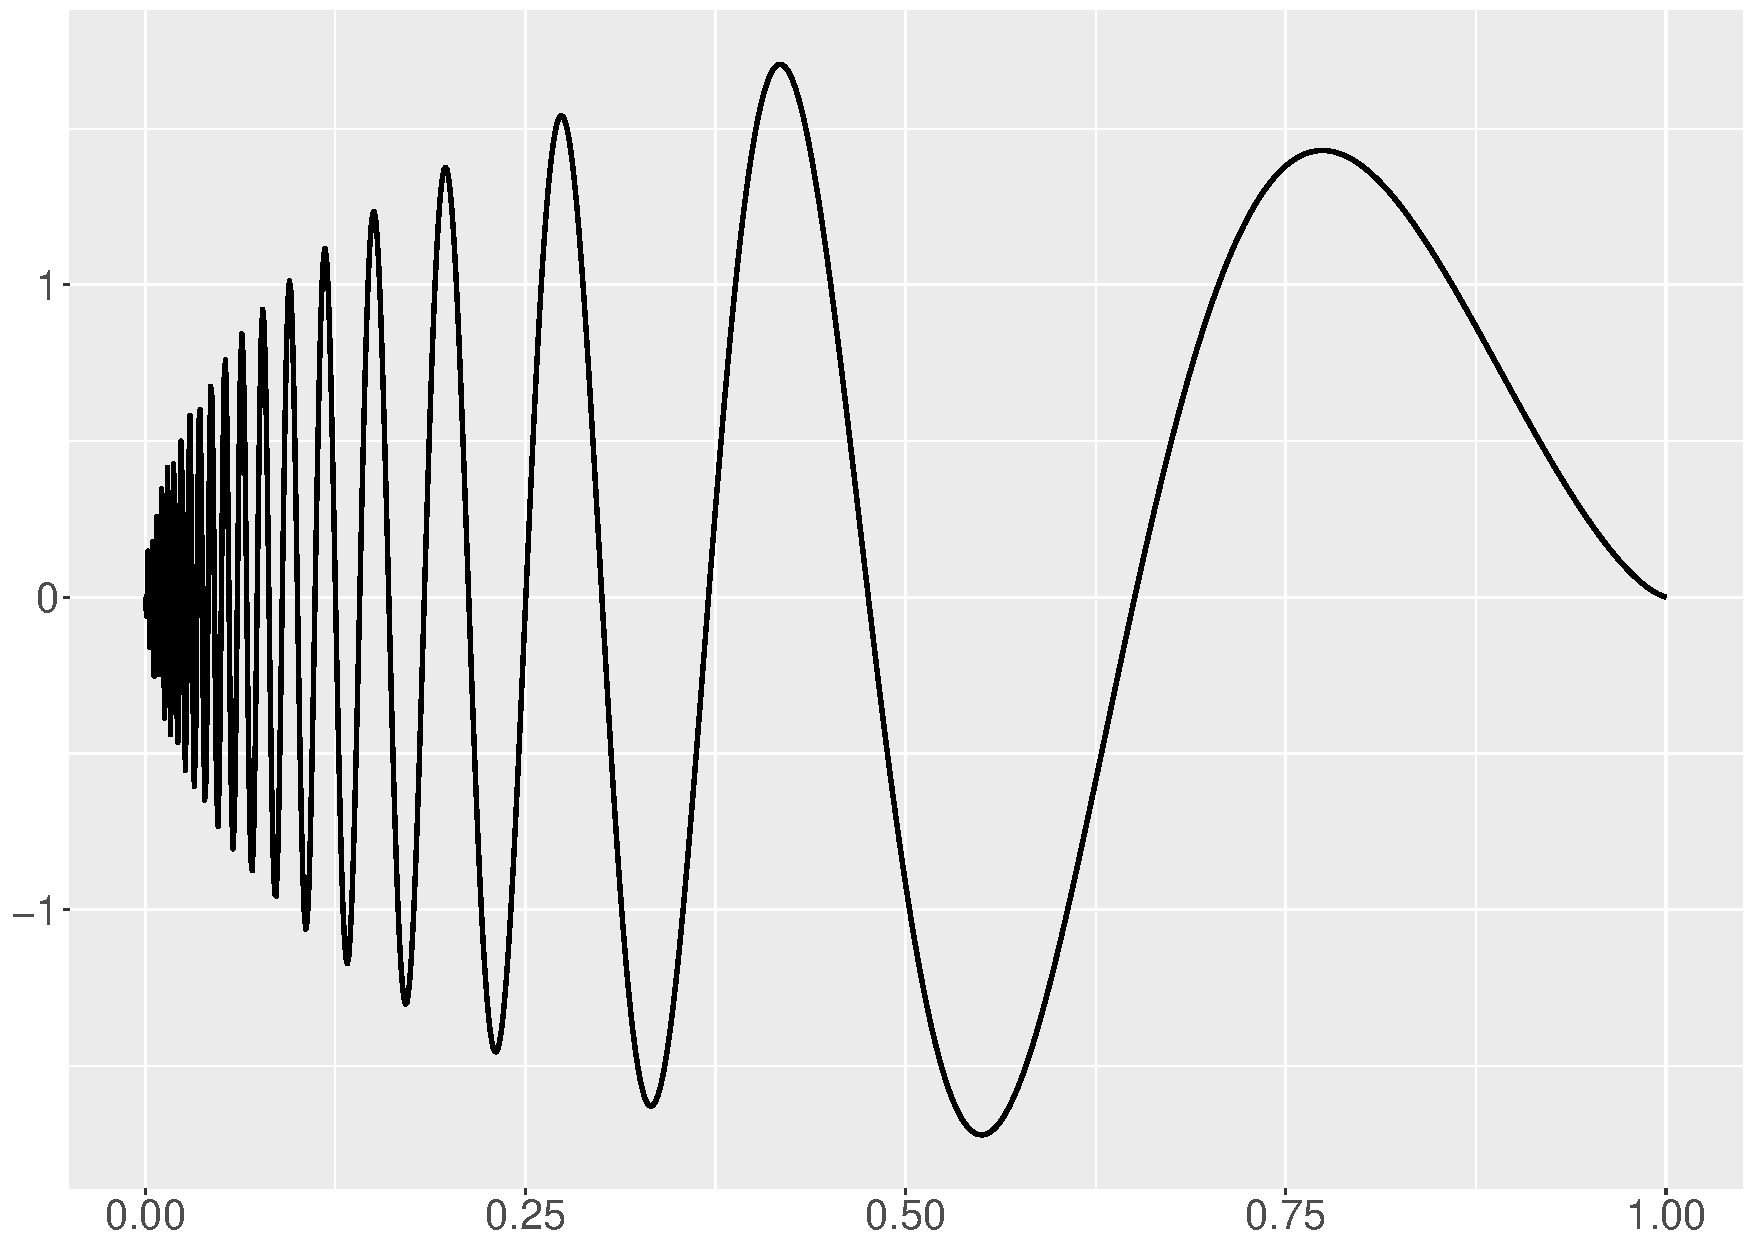
\includegraphics[width=\linewidth,height=0.45\textwidth]{Chapters/02TractorSplineTheory/plot/ggplot/ggDoppler.pdf}
    \caption{True \textit{Doppler} function}
    \end{subfigure}%
    \begin{subfigure}{0.45\textwidth}
    \centering
    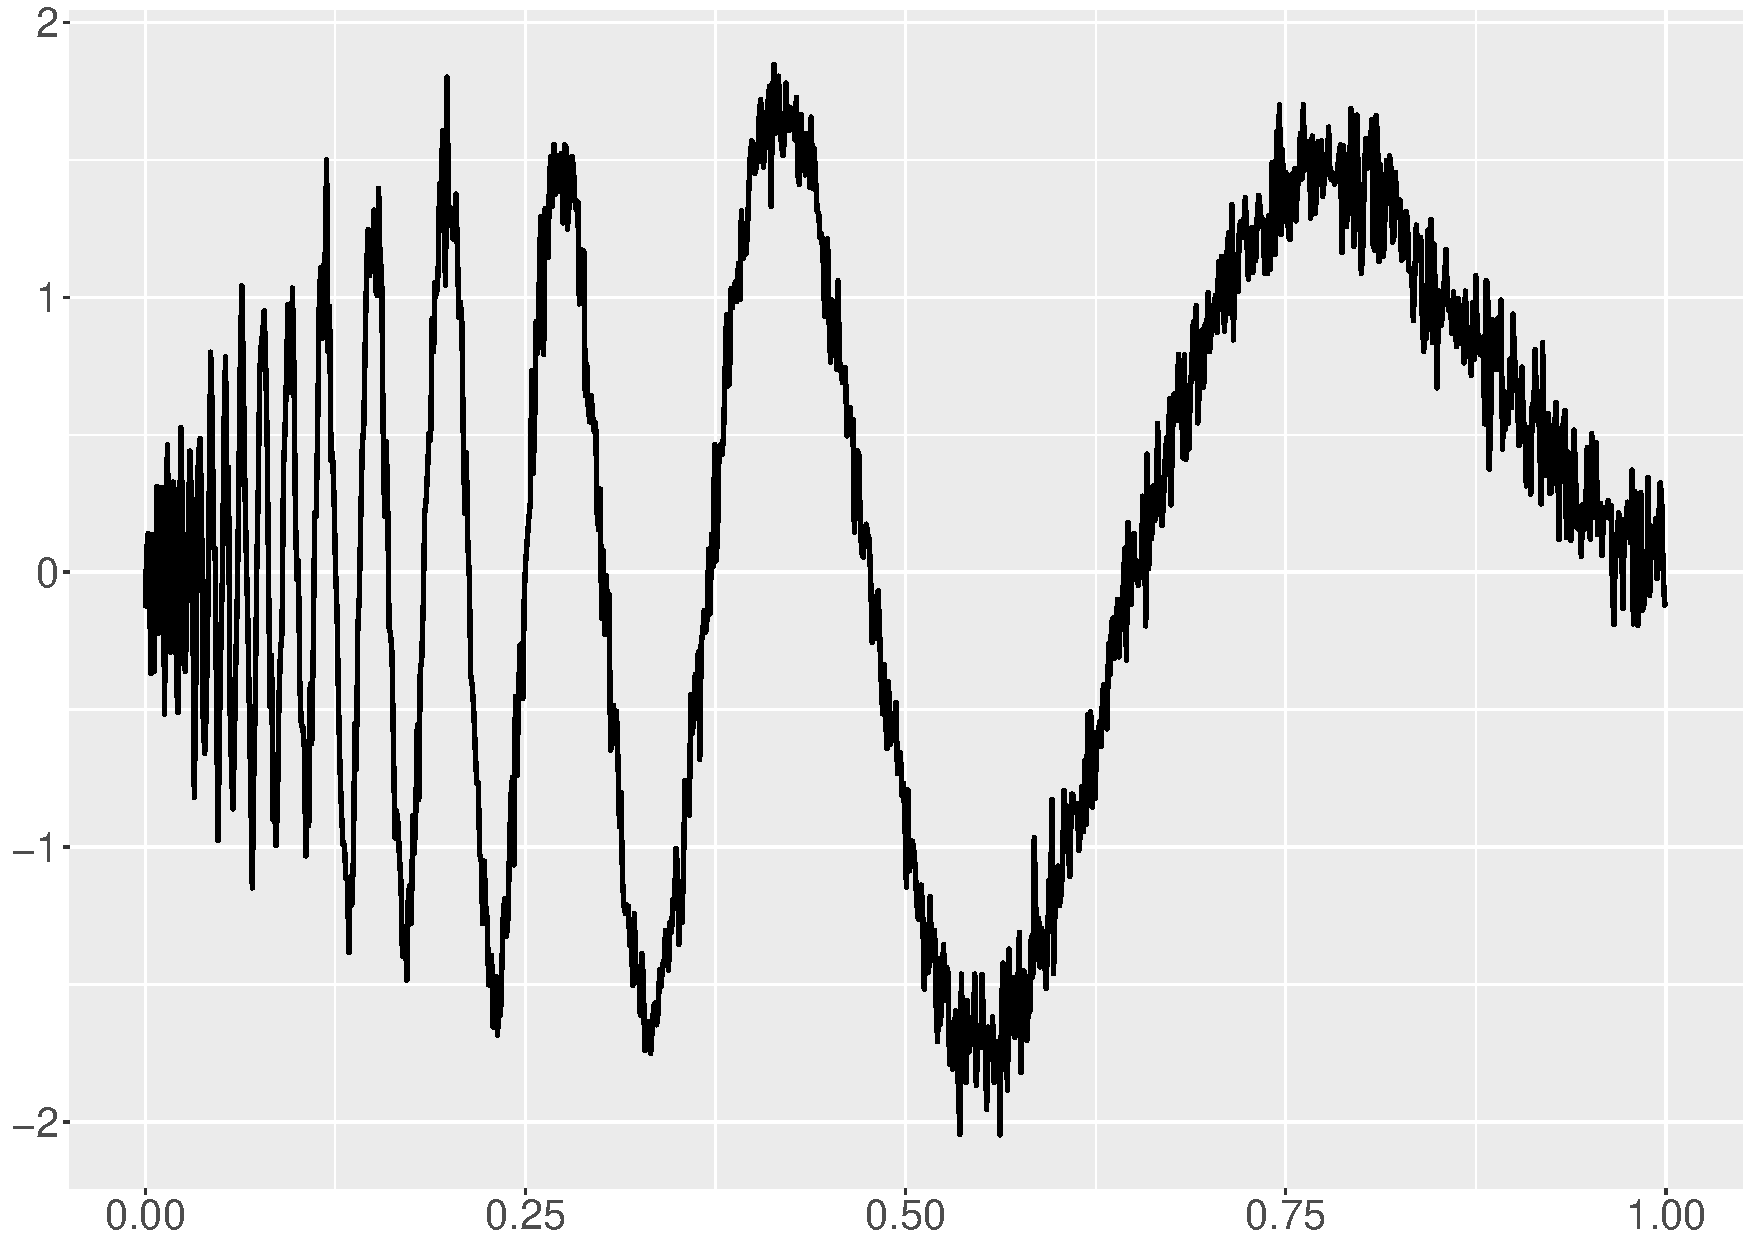
\includegraphics[width=\linewidth,,height=0.45\textwidth]{Chapters/02TractorSplineTheory/plot/ggplot/ggDopplerNoise.pdf}
    \caption{Noisy \textit{Doppler} at \textit{SNR}=7}
    \end{subfigure}
    \begin{subfigure}{0.45\textwidth}
    \centering
    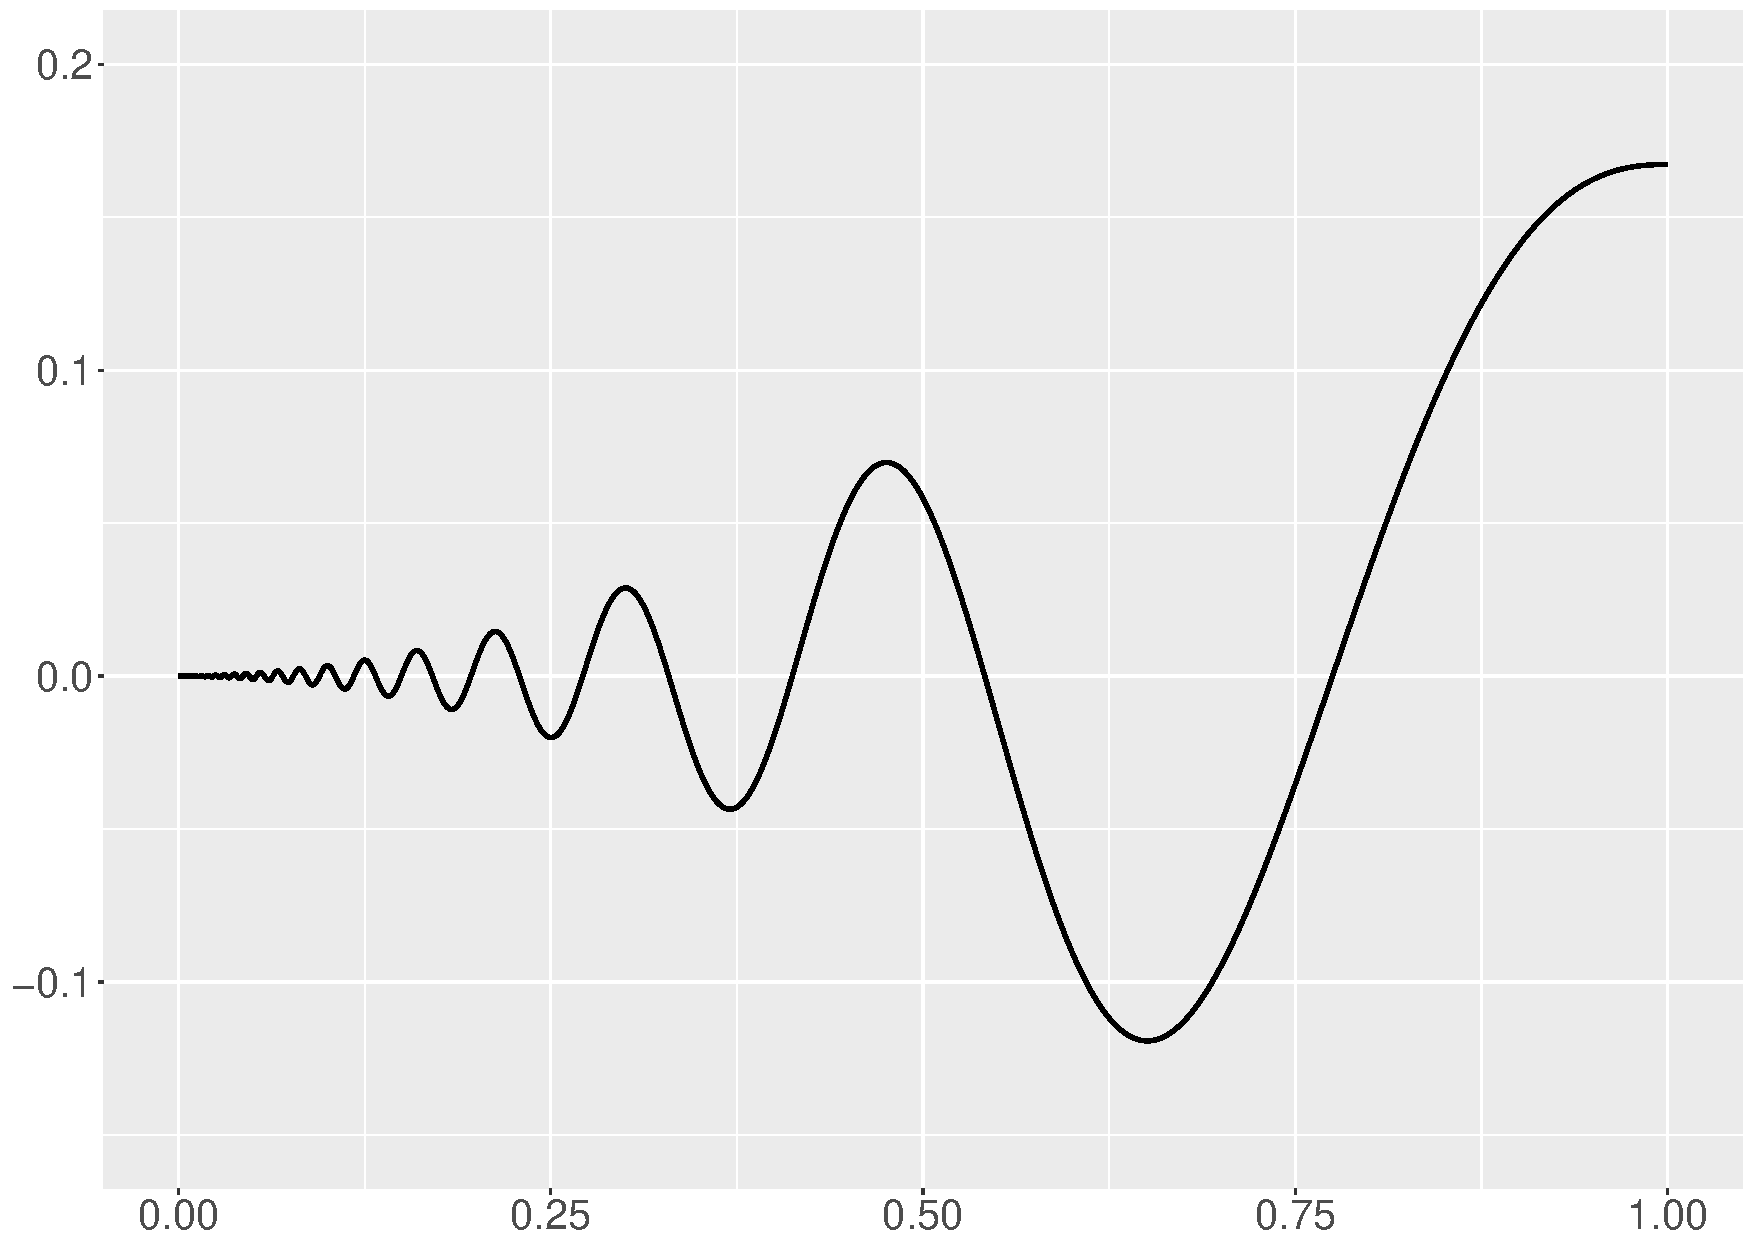
\includegraphics[width=\linewidth,height=0.45\textwidth]{Chapters/02TractorSplineTheory/plot/ggplot/ggDopplerPosition.pdf}
    \caption{Generated positions}
    \end{subfigure}
    \begin{subfigure}{0.45\textwidth}
    \centering
    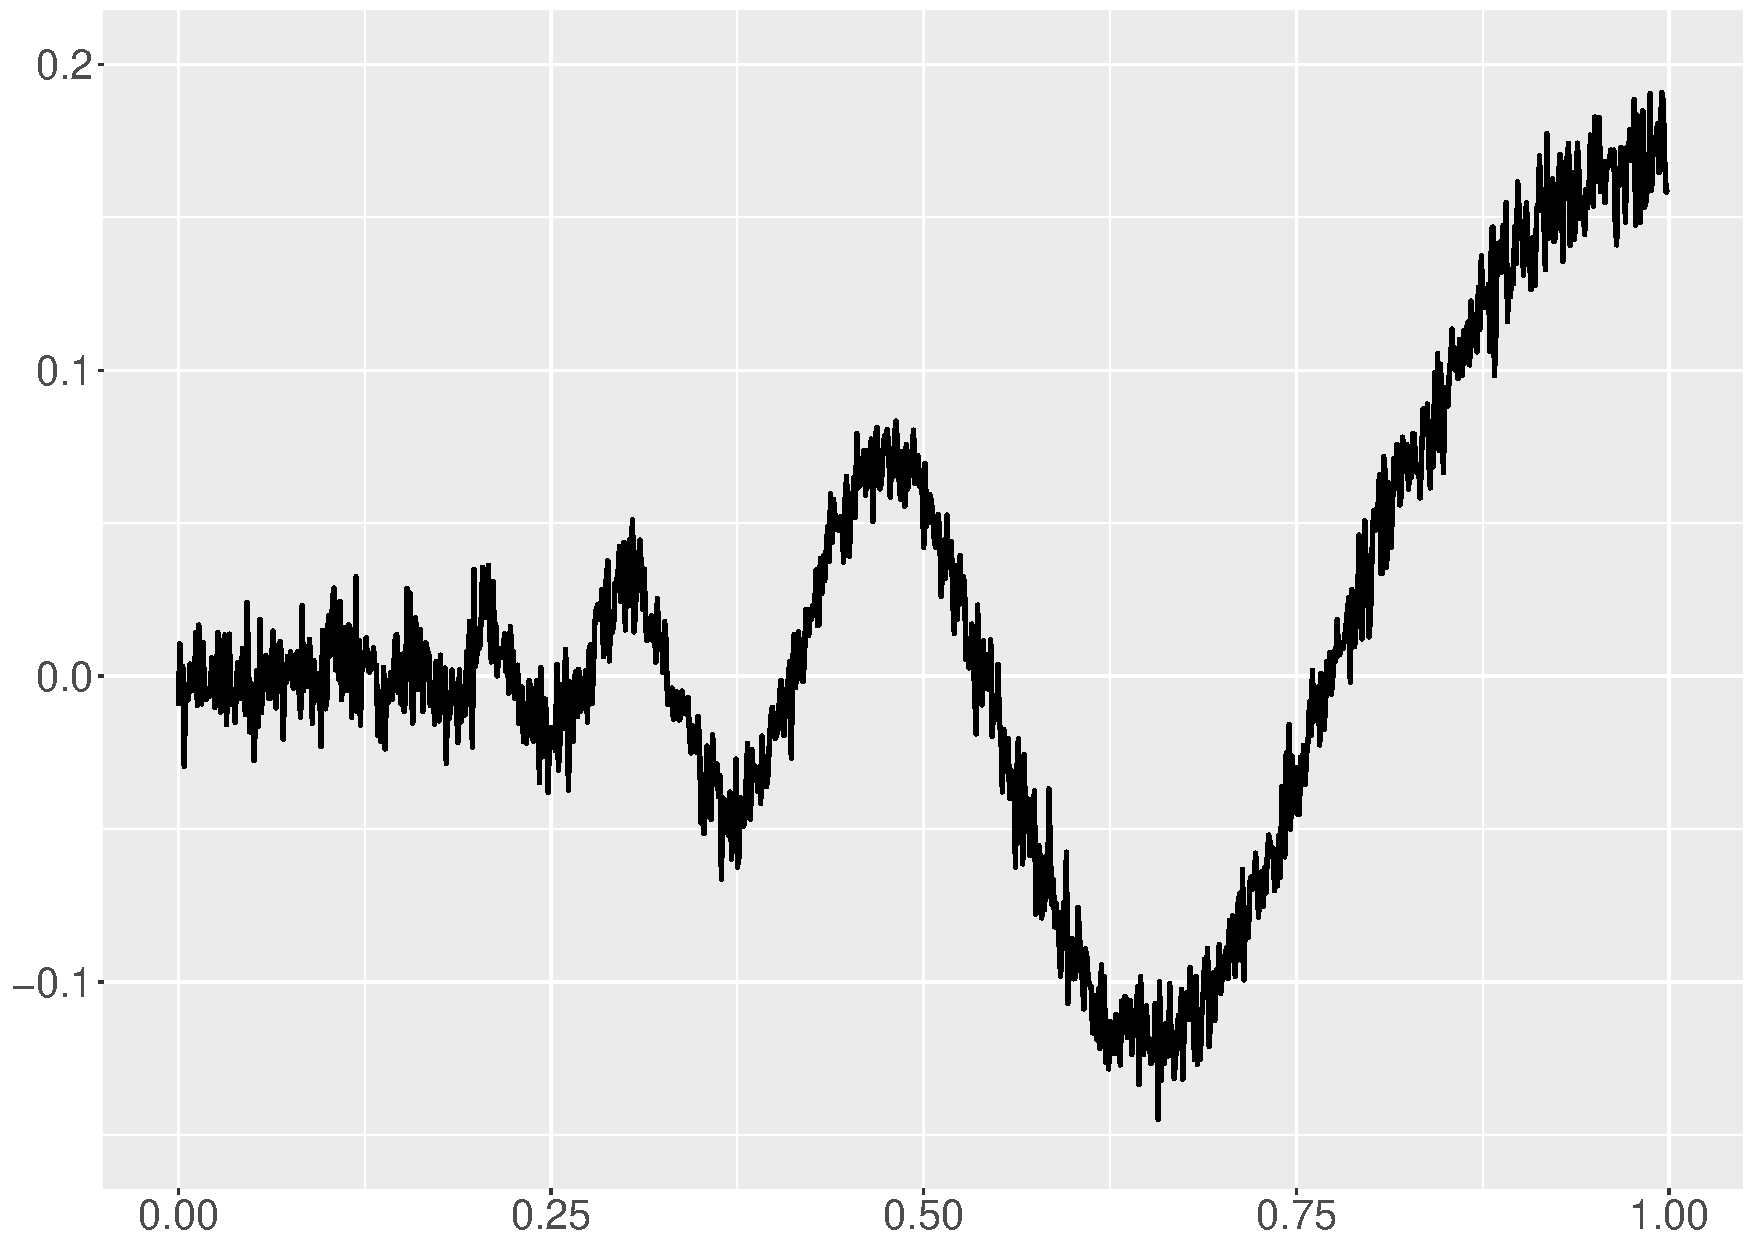
\includegraphics[width=\linewidth,height=0.45\textwidth]{Chapters/02TractorSplineTheory/plot/ggplot/ggDopplerPositionNoise.pdf}
    \caption{Noisy position at \textit{SNR}=7}
    \end{subfigure}
    \begin{subfigure}{0.45\textwidth}
    \centering
    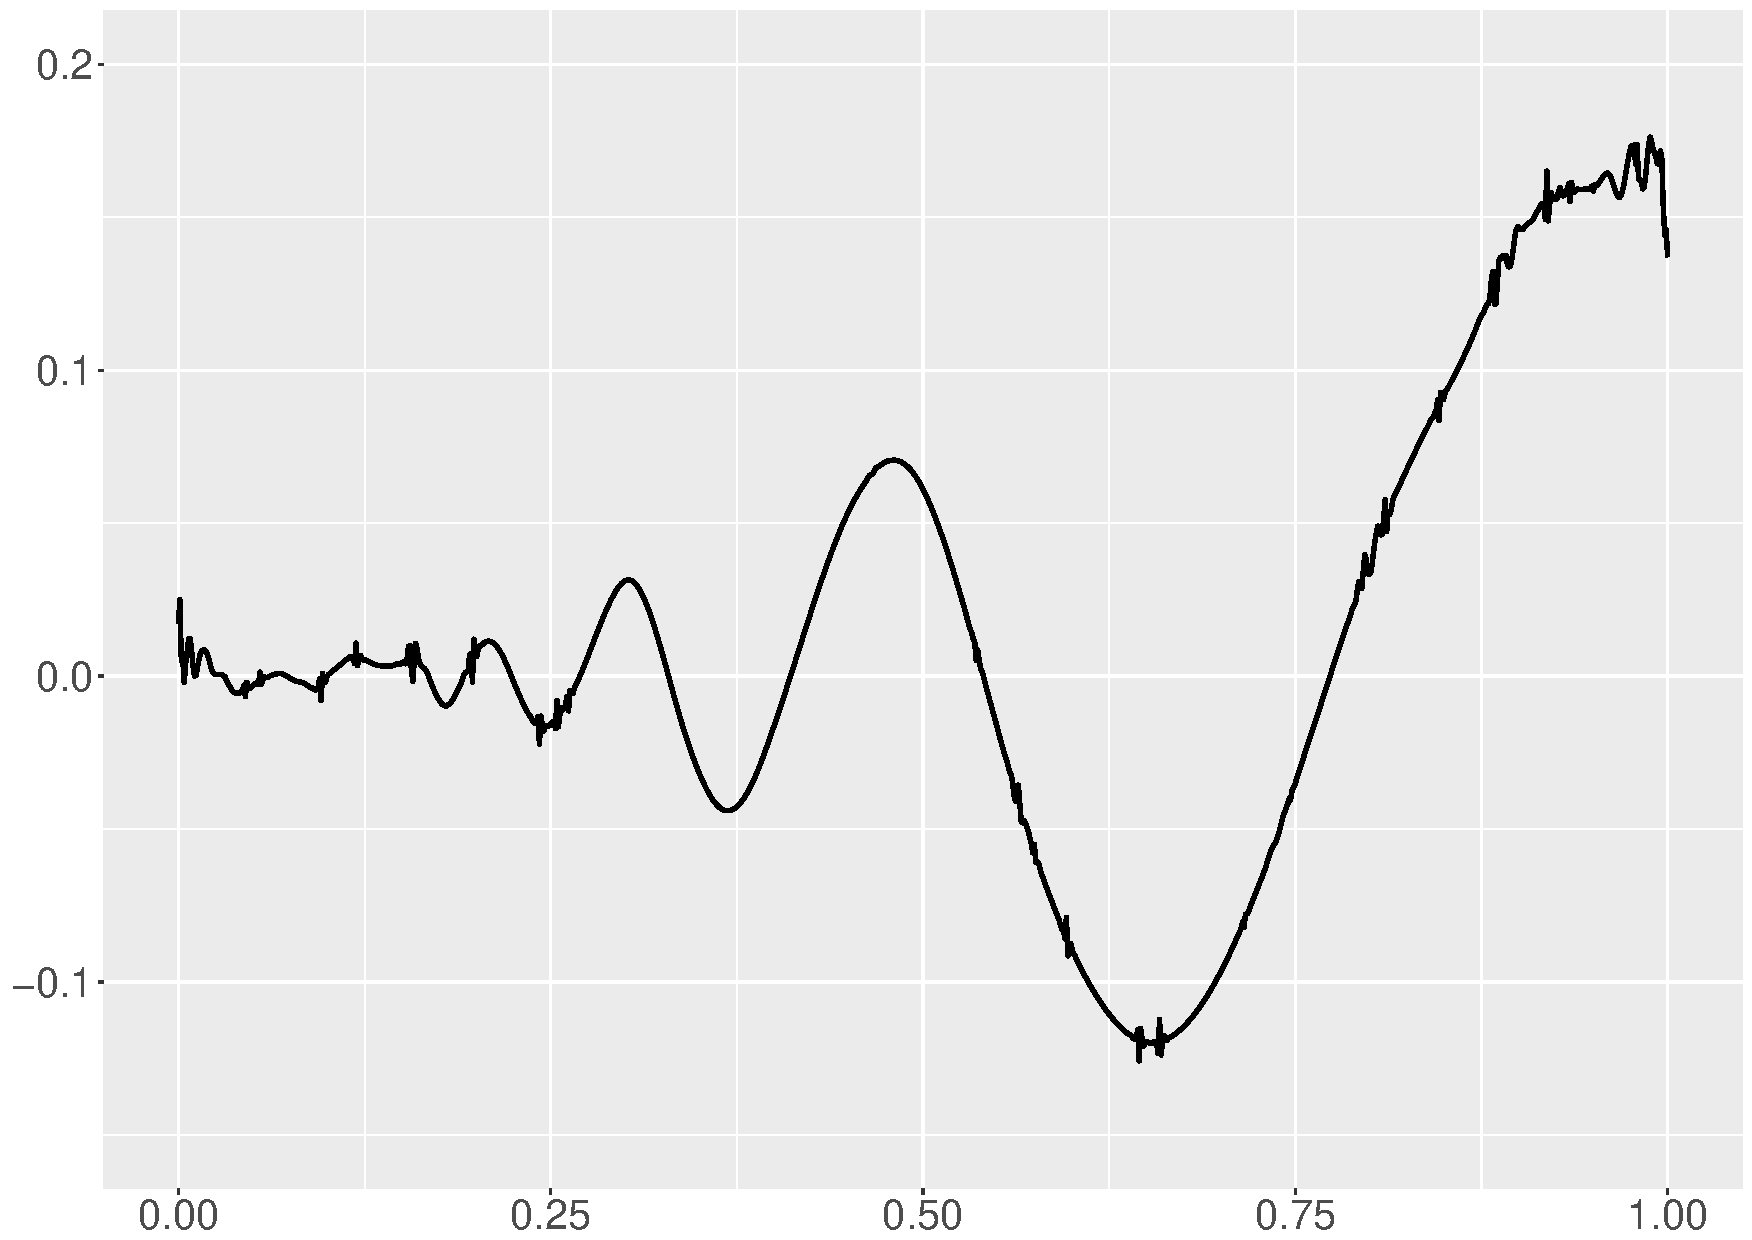
\includegraphics[width=\linewidth,height=0.45\textwidth]{Chapters/02TractorSplineTheory/plot/ggplot/ggDopplerSure.pdf}
    \caption{Reconstruction from Wavelet by sure threshold}
    \end{subfigure}
    \begin{subfigure}{0.45\textwidth}
    \centering
    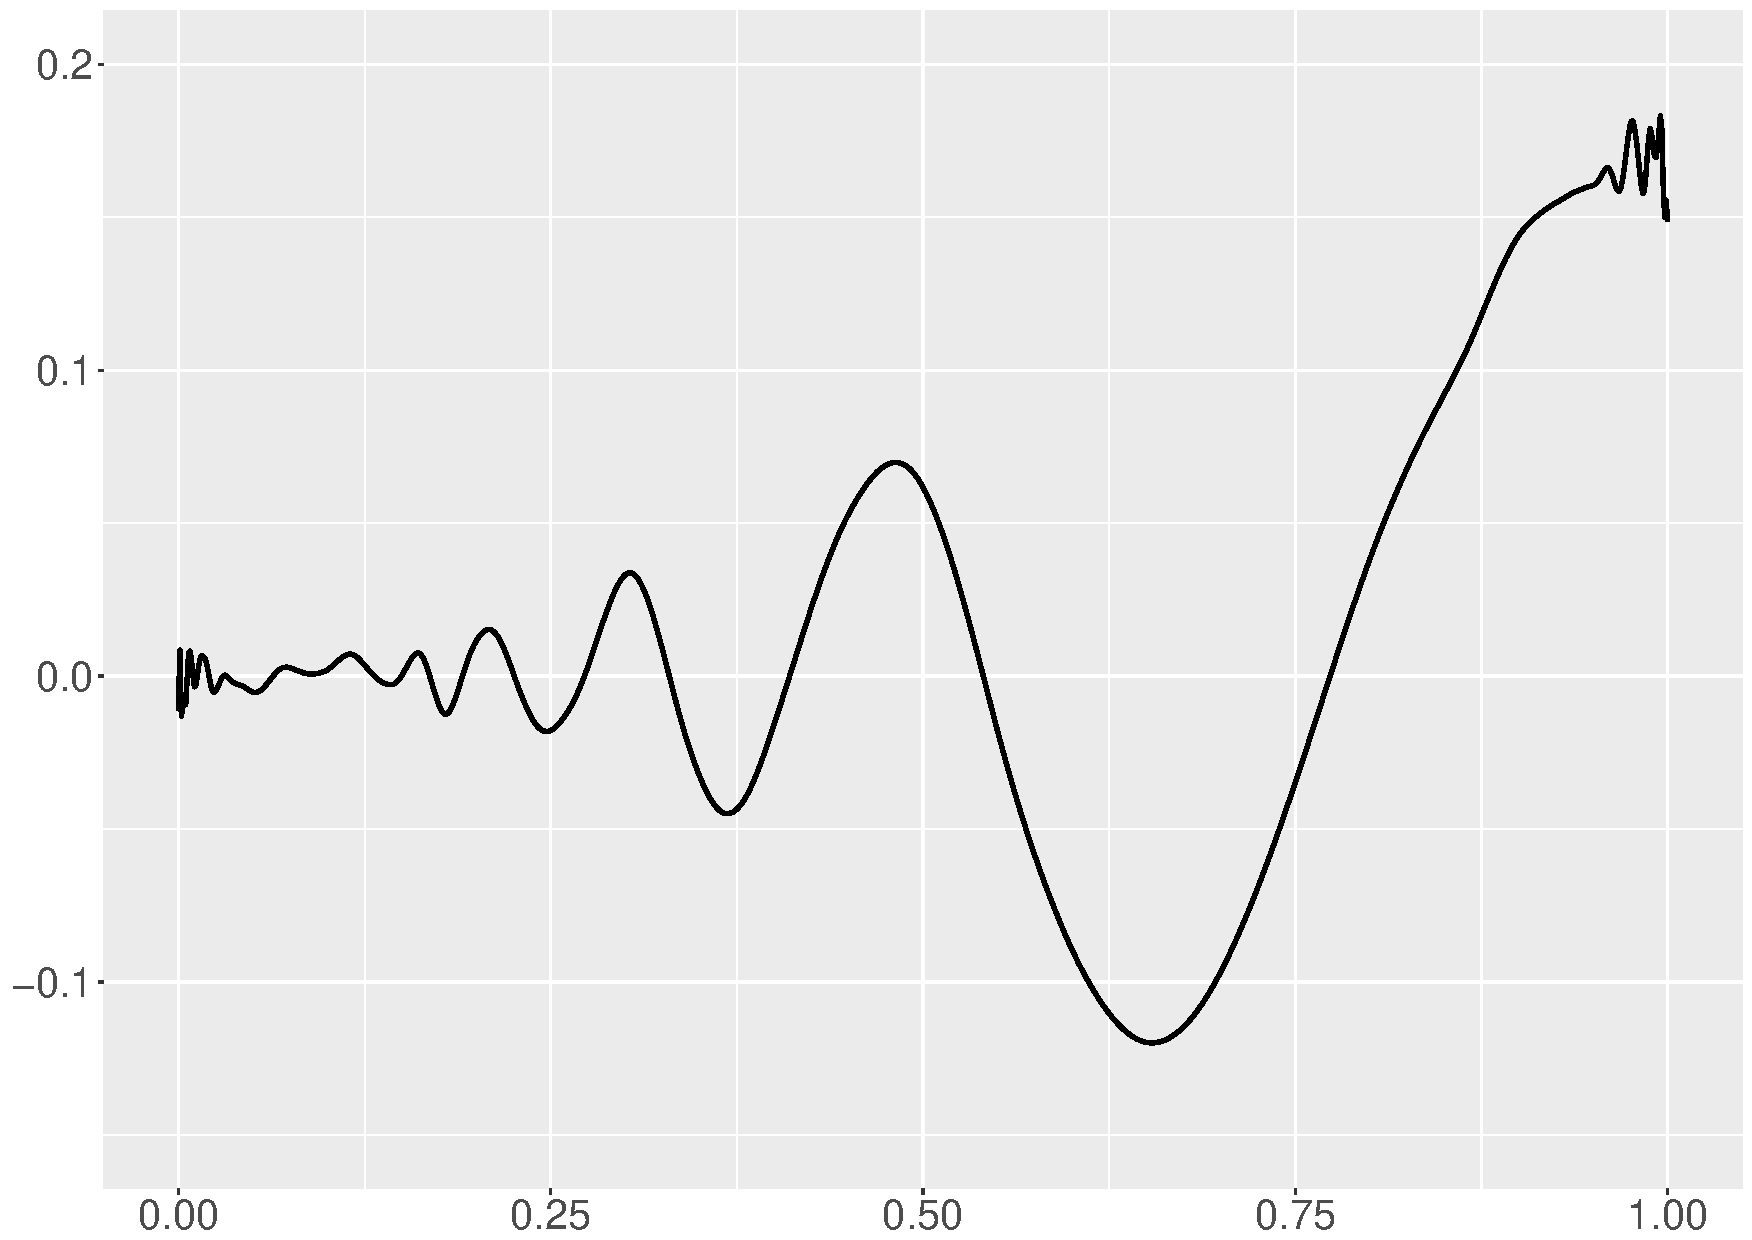
\includegraphics[width=\linewidth,height=0.45\textwidth]{Chapters/02TractorSplineTheory/plot/ggplot/ggDopplerBayes.pdf}
    \caption{Reconstruction from Wavelet by BayesThresh approach}
    \end{subfigure}
    \begin{subfigure}{0.45\textwidth}
    \centering
    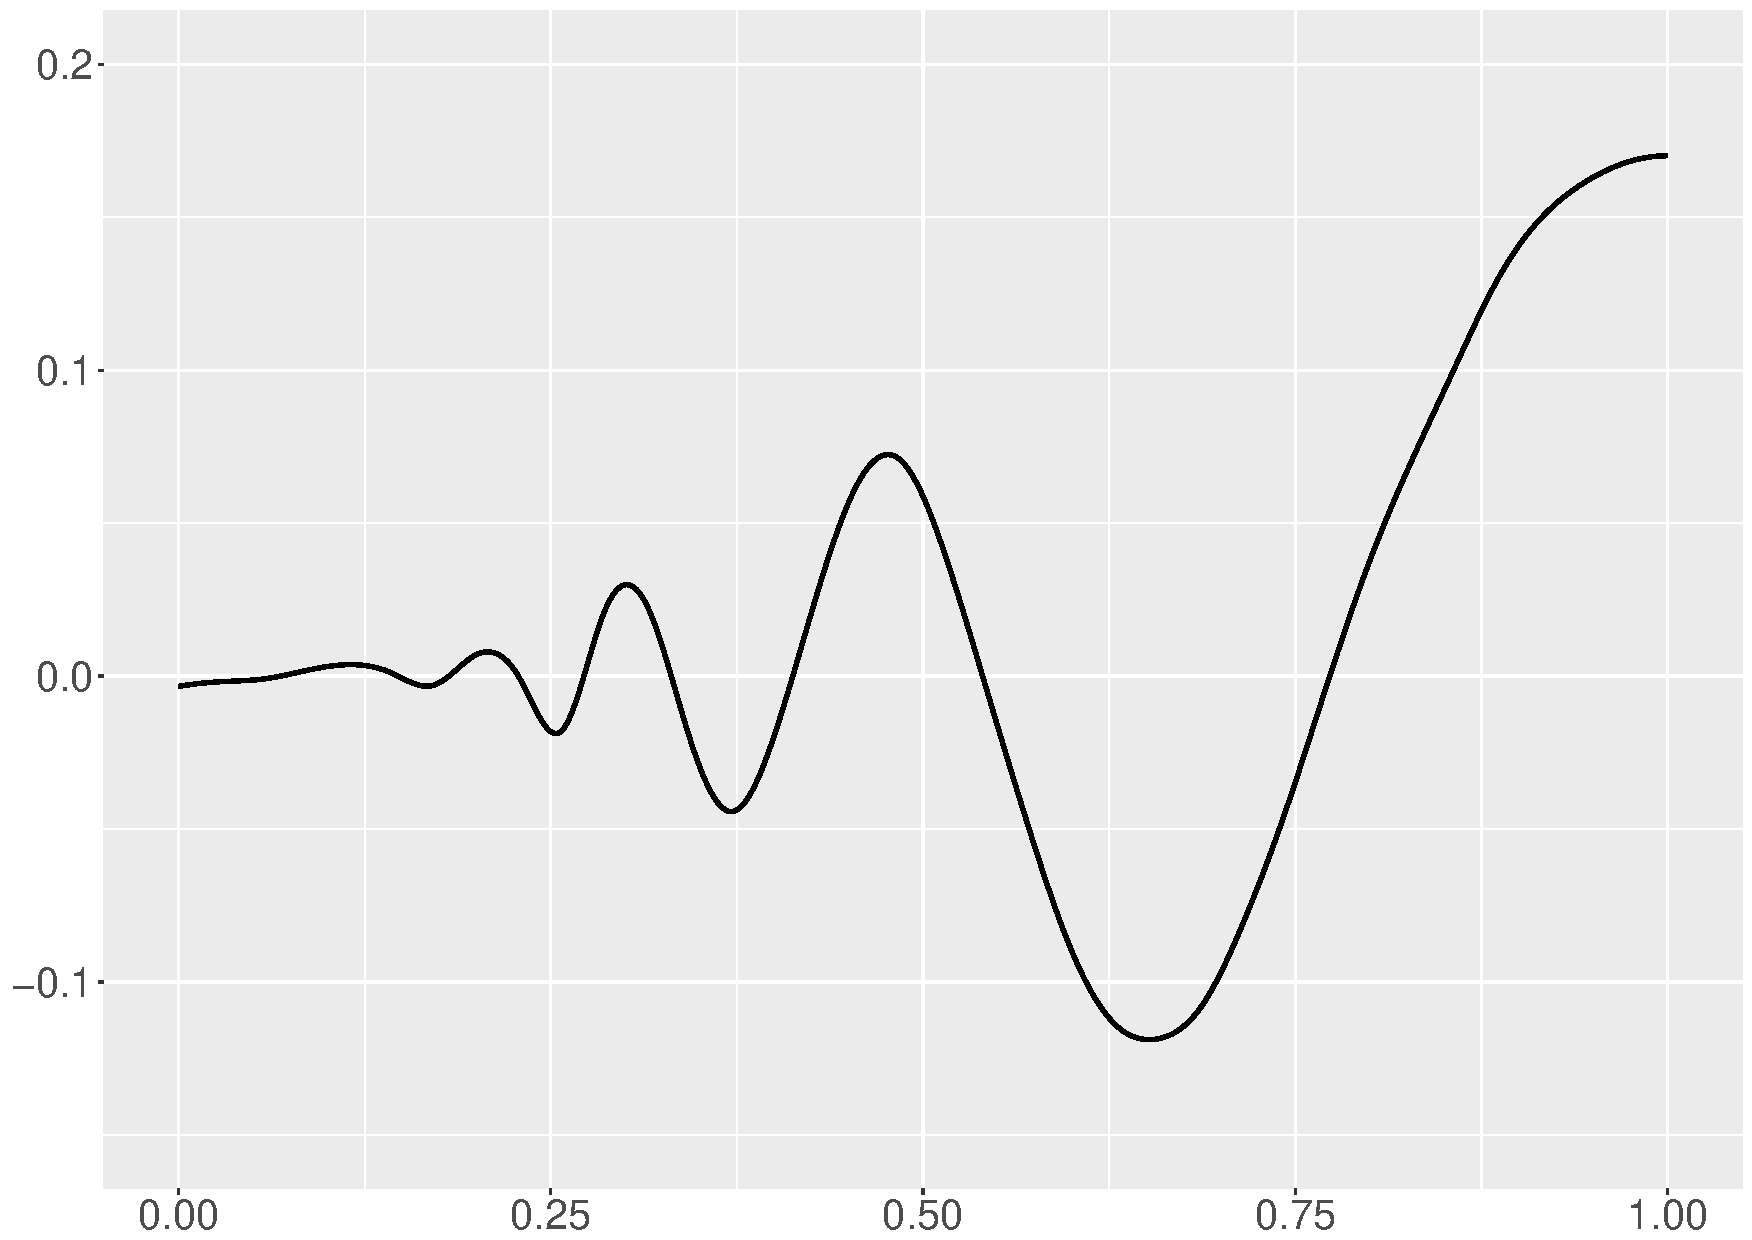
\includegraphics[width=\linewidth,height=0.45\textwidth]{Chapters/02TractorSplineTheory/plot/ggplot/ggDopplerPSpline.pdf}
    \caption{Reconstruction by P-spline \\\mbox{  } }
    \end{subfigure}
    \begin{subfigure}{0.45\textwidth}
    \centering
    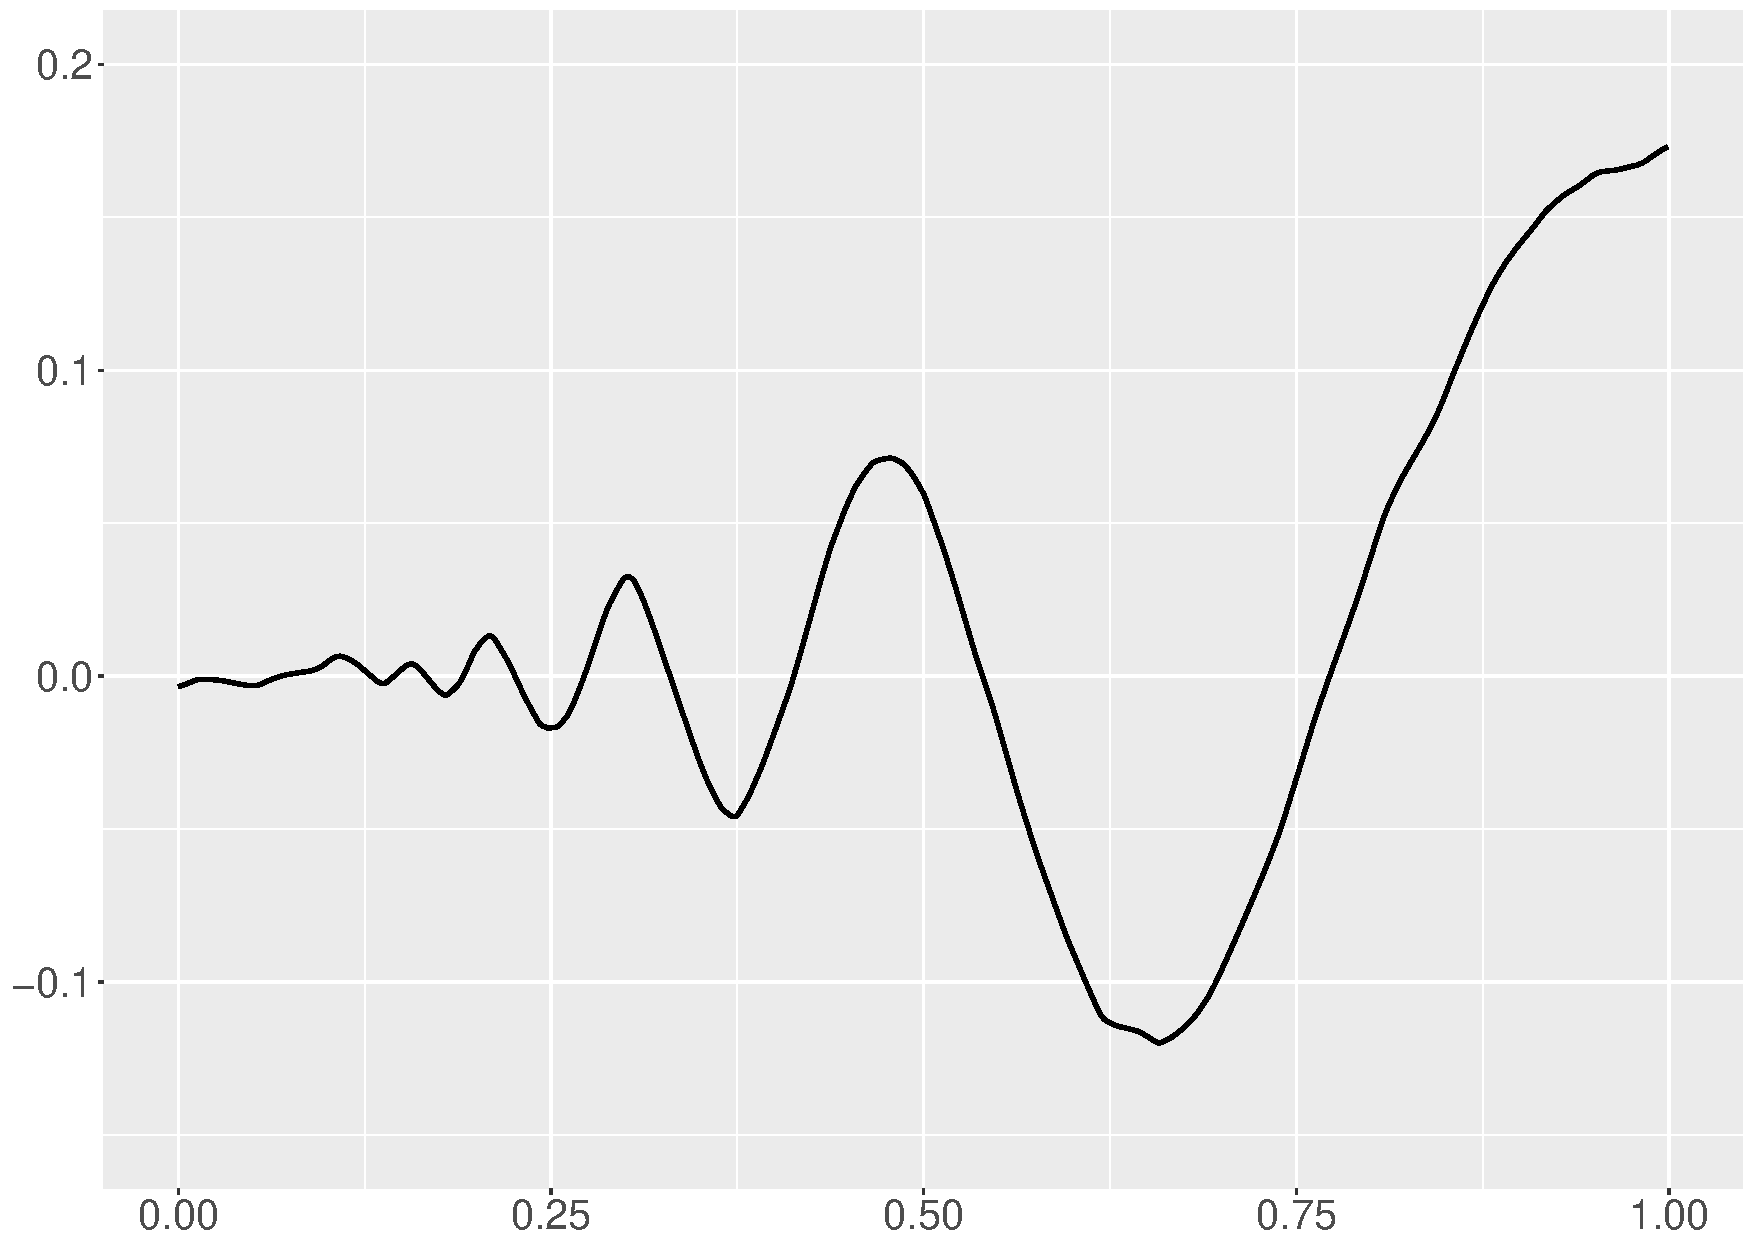
\includegraphics[width=\linewidth,height=0.45\textwidth]{Chapters/02TractorSplineTheory/plot/ggplot/ggDopplerGamma.pdf}
    \caption{Reconstruction by V-spline setting $\gamma=0$}
    \end{subfigure}
  \begin{subfigure}{0.45\textwidth}
    \centering
    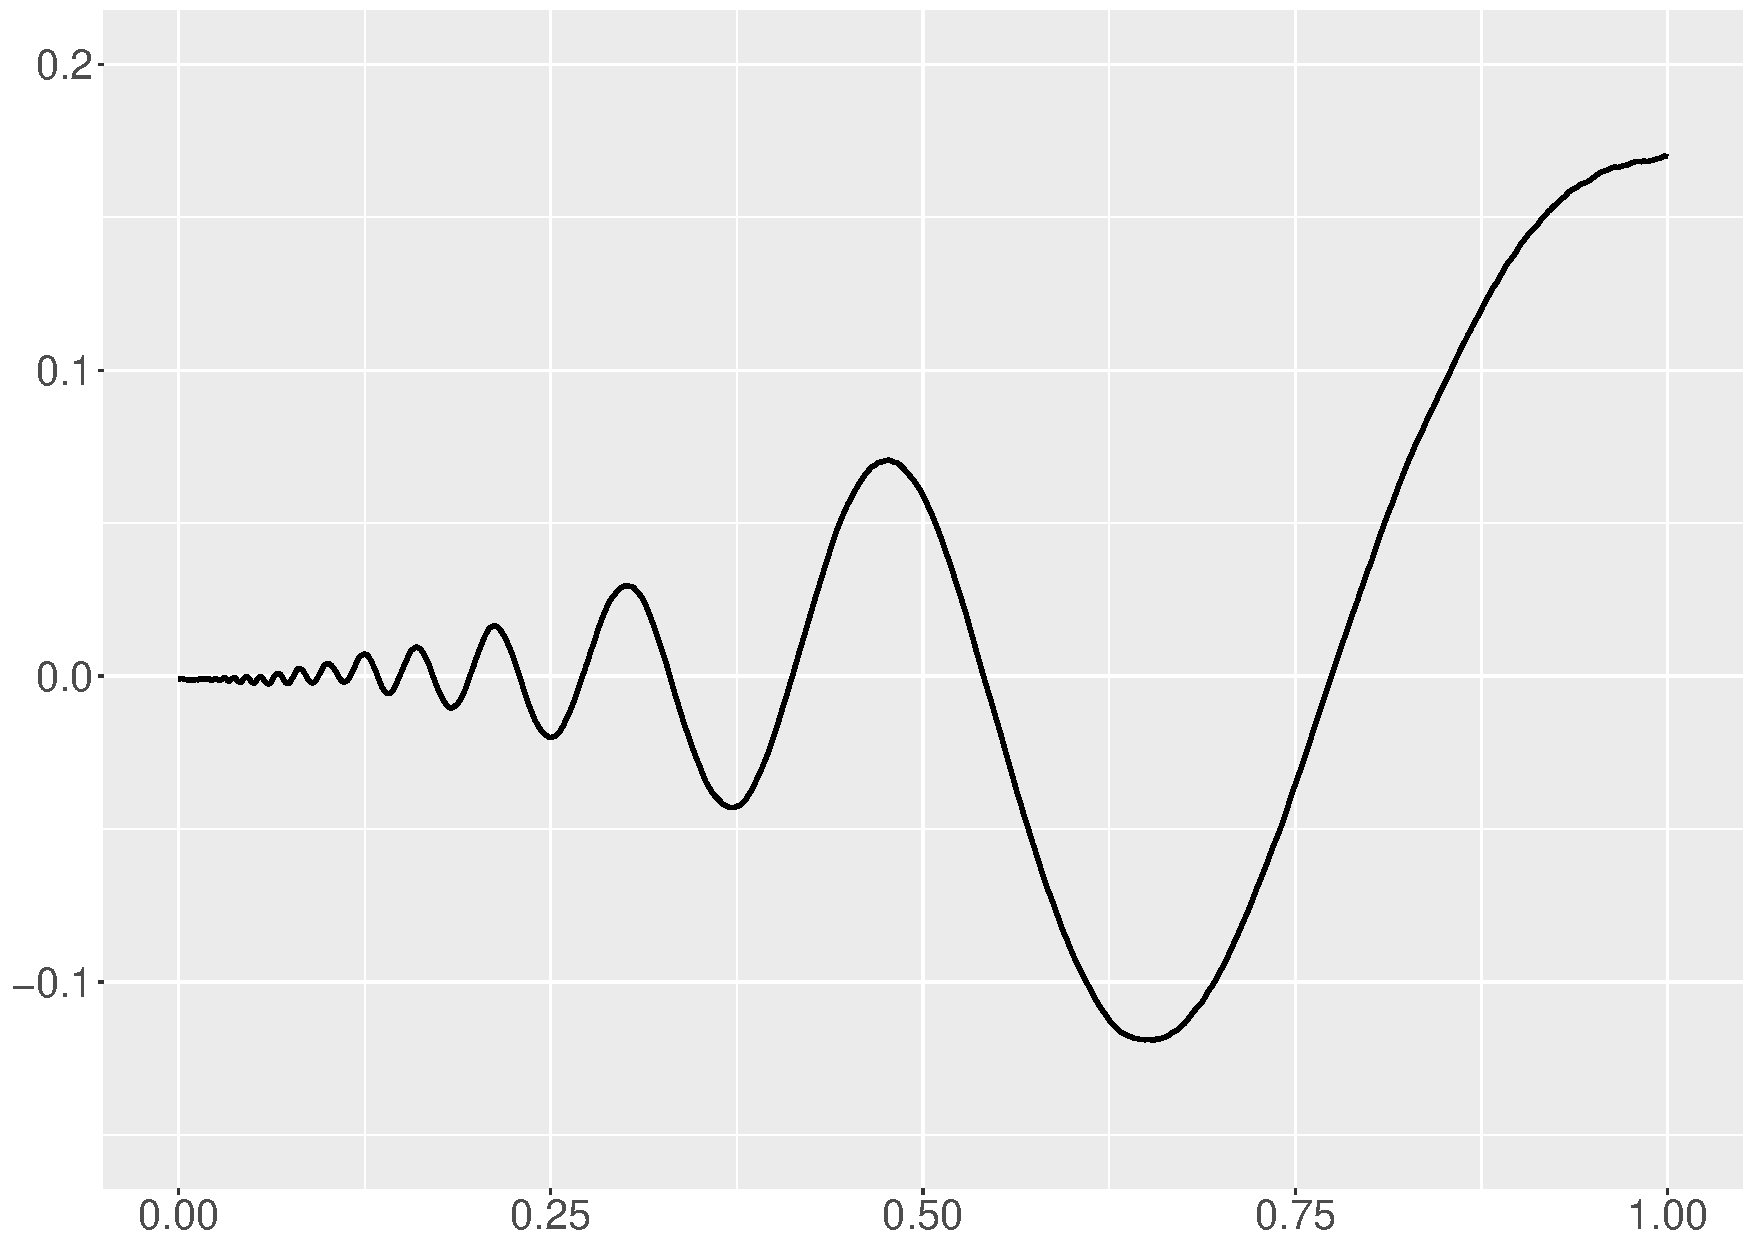
\includegraphics[width=\linewidth,height=0.45\textwidth]{Chapters/02TractorSplineTheory/plot/ggplot/ggDopplerTractorAPT.pdf}
    \caption{Reconstruction by V-spline with conventional penalty term}
    \end{subfigure}
    \begin{subfigure}{0.45\textwidth}
    \centering
    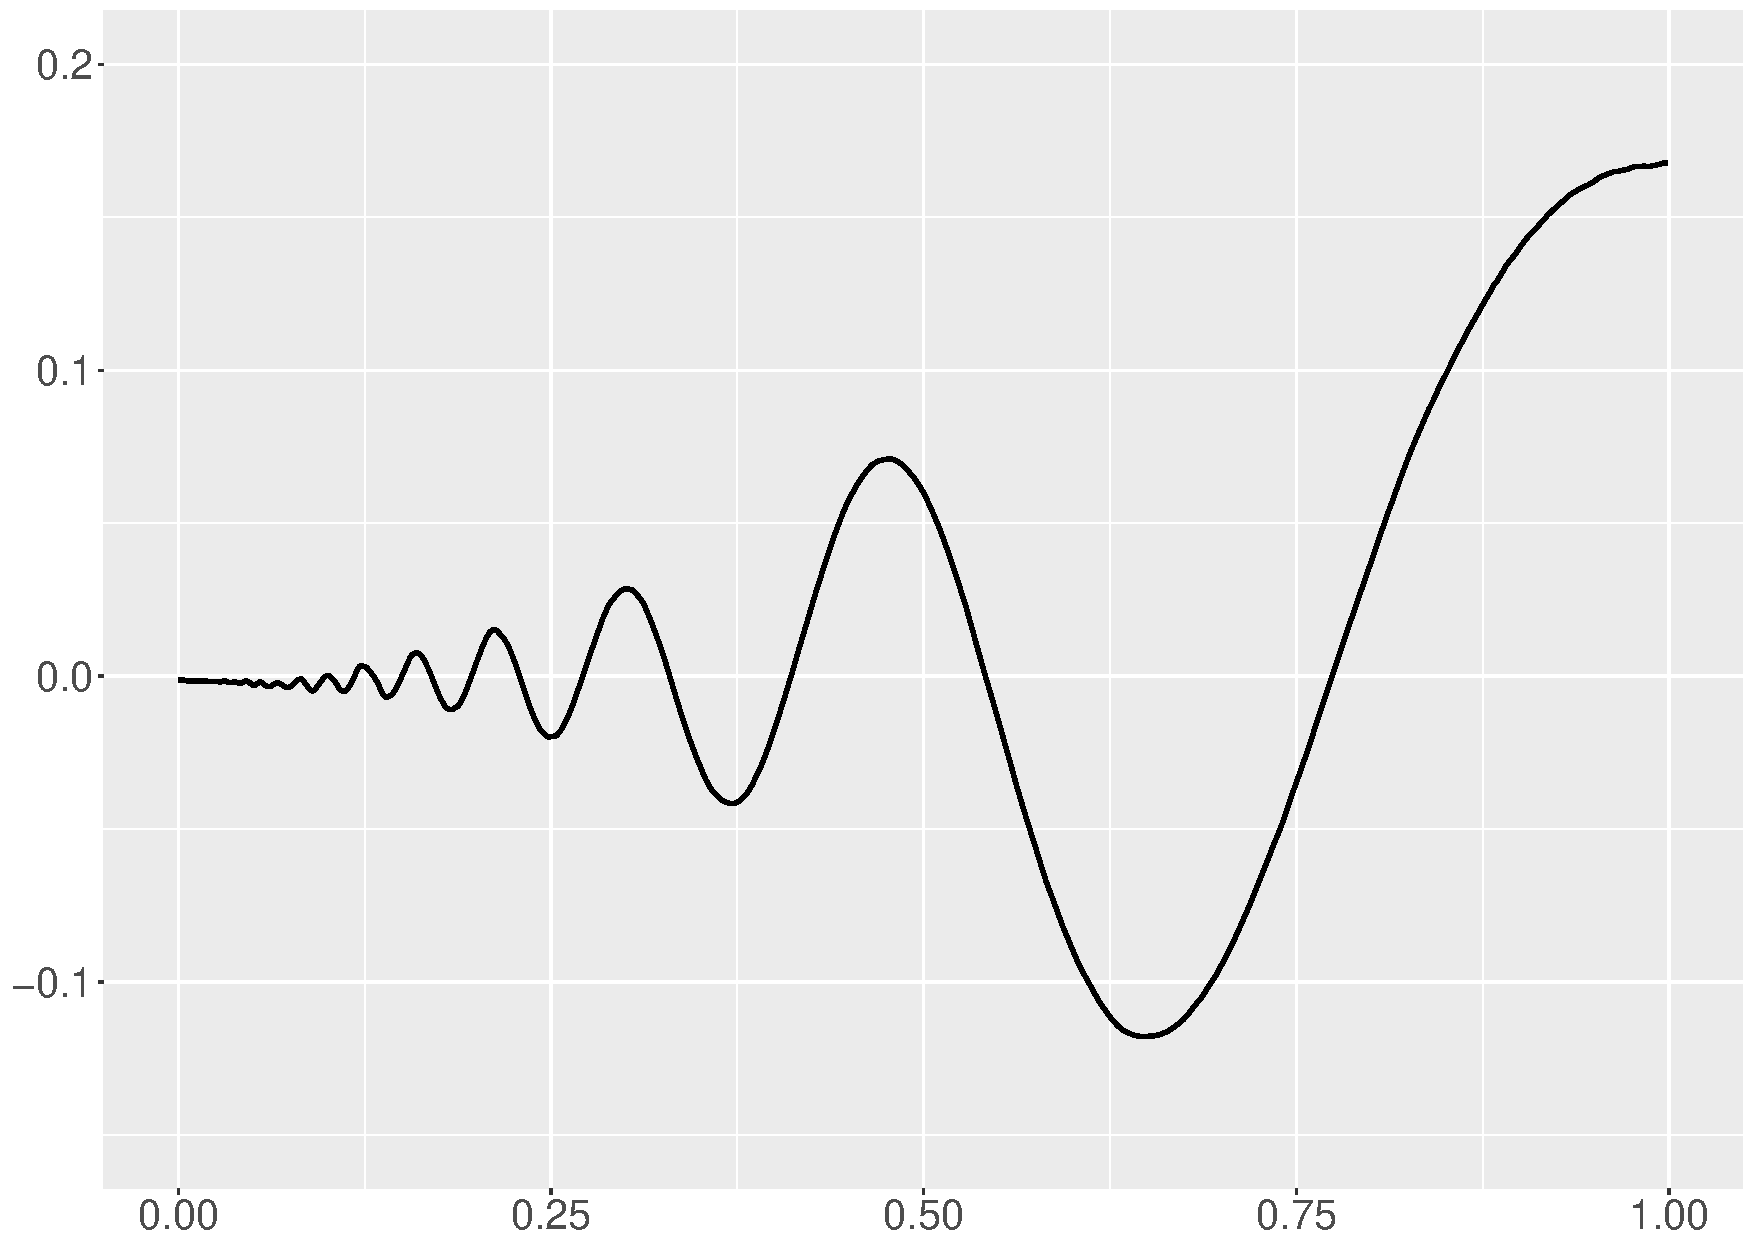
\includegraphics[width=\linewidth,height=0.45\textwidth]{Chapters/02TractorSplineTheory/plot/ggplot/ggDopplerTractor.pdf}
    \caption{Reconstruction by the proposed V-spline.}
    \end{subfigure}
\caption{Numerical example: $\textit{Doppler}$. Comparison of different reconstruction methods with simulated data}\label{num4}
 \end{figure}

By comparing, we can see that all these methods can rebuild up the skeleton of generated trajectory. \textit{Wavelet(sure)} method has more wiggles in interior interval than \textit{Wavelet(BayesThresh)} does, and the latter one becomes fluctuation near boundary knots. \textit{P-spline} gives a smoother fitting than wavelets, but the drawback is lack of specific details. V-spline without velocity loses some information, as can be seen from \textit{Blocks} and \textit{Bumps} where there should be a straight line. V-spline without adjusted penalty term gets over-fitting when the direction changes more frequently than normal, although it catches specific feature in \textit{HeaviSine}. The proposed V-spline performs much better than other methods and returns the near-true trajectory reconstructions.  



%and is larger when the function trying to change directions. We only have a couple of large penalty terms in $\textit{Blocks}$ and $\textit{Bumps}$ function, as most of the time they were moving in straight line. More curves are in $\textit{HeaviSine}$ and $\textit{Doppler}$ functions, so the penalty term try to catch more information and ignore noises. 
%\begin{figure}
%  \centering
%         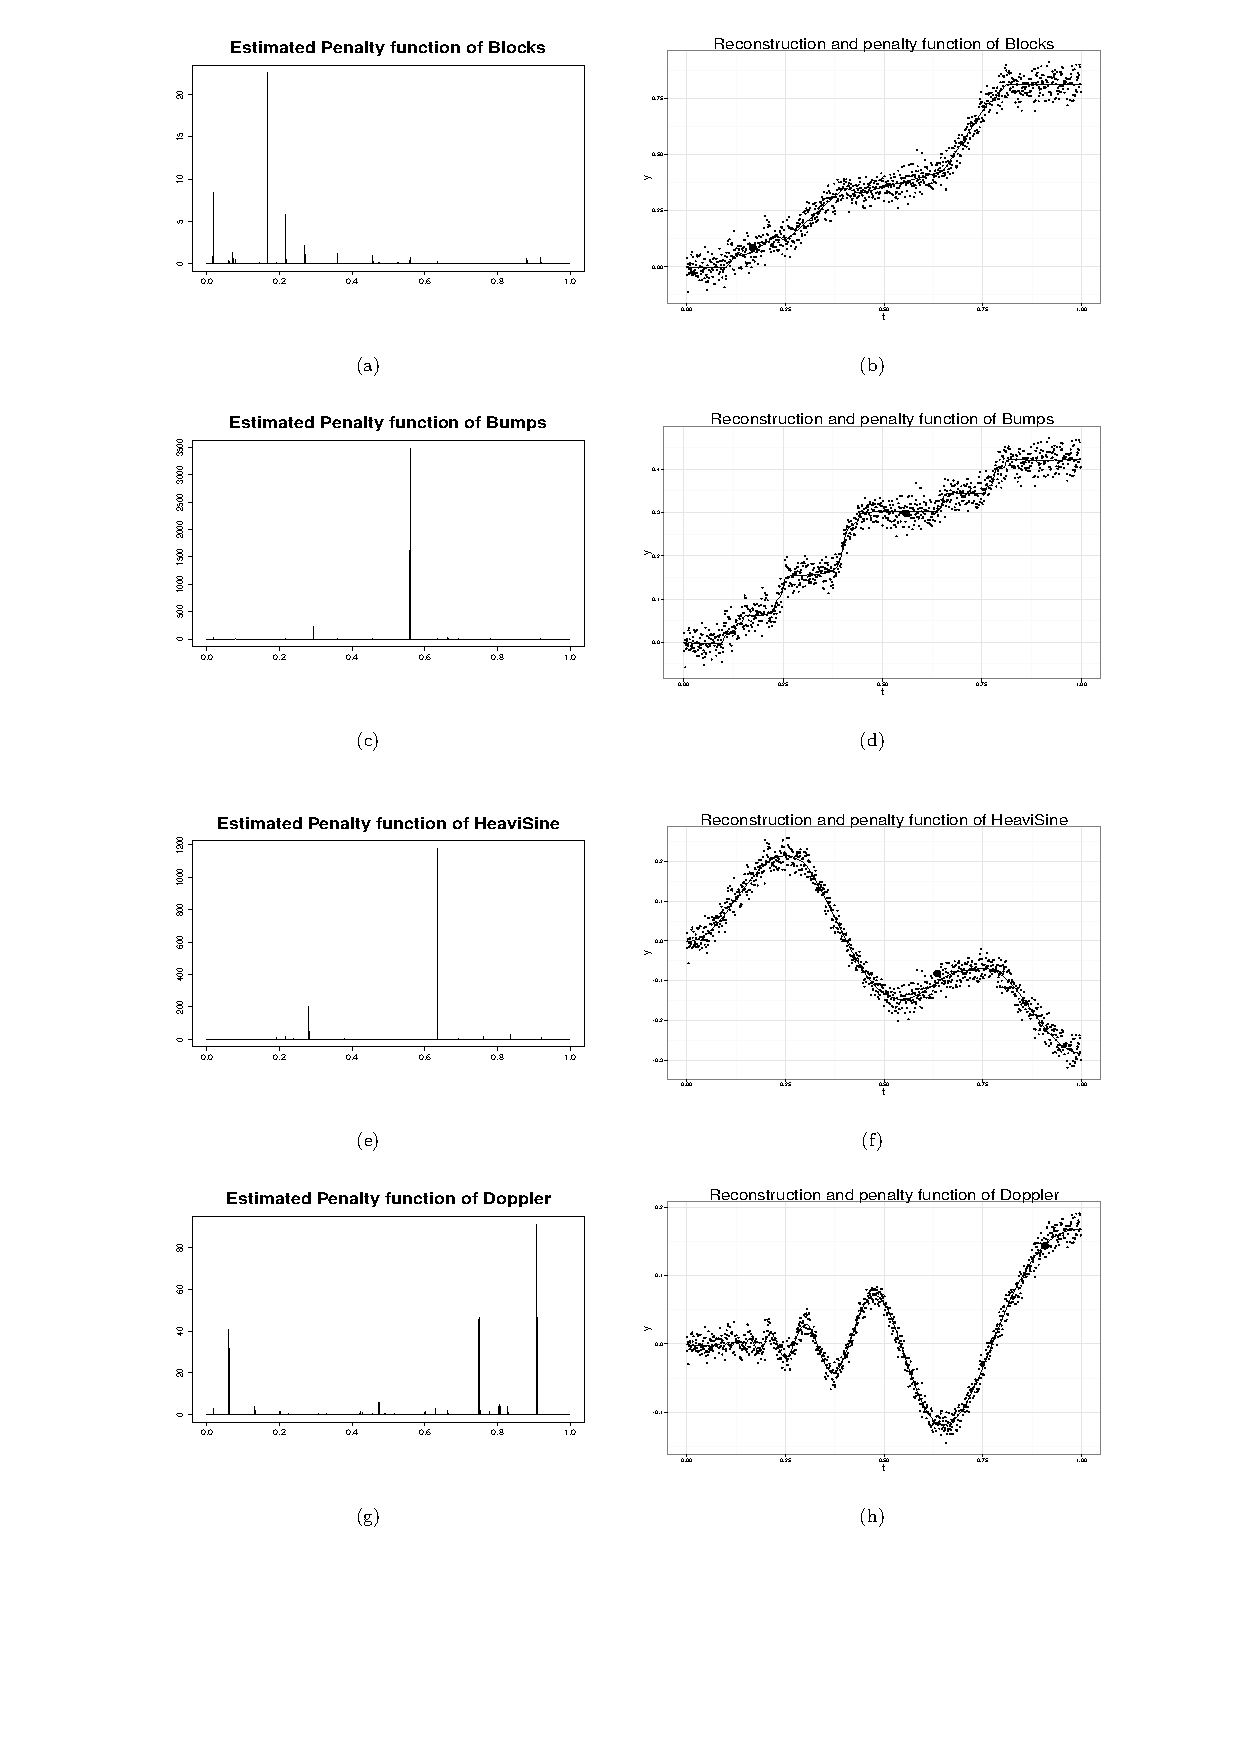
\includegraphics[width=\textwidth,height=14cm]{Chapters/02TractorSplineTheory/plot/penalty08} 
%  \caption{Estimated penalty functions. Left side shows how the value of $\lambda(t)$ changes on the interval. Right side projects $\lambda(t)$ into reconstructions. The bigger the blacks dots present, the larger the penalty values are.}\label{numpenalty}
%\end{figure}

\begin{figure}
    \centering
    \begin{subfigure}{\textwidth}
    \centering
    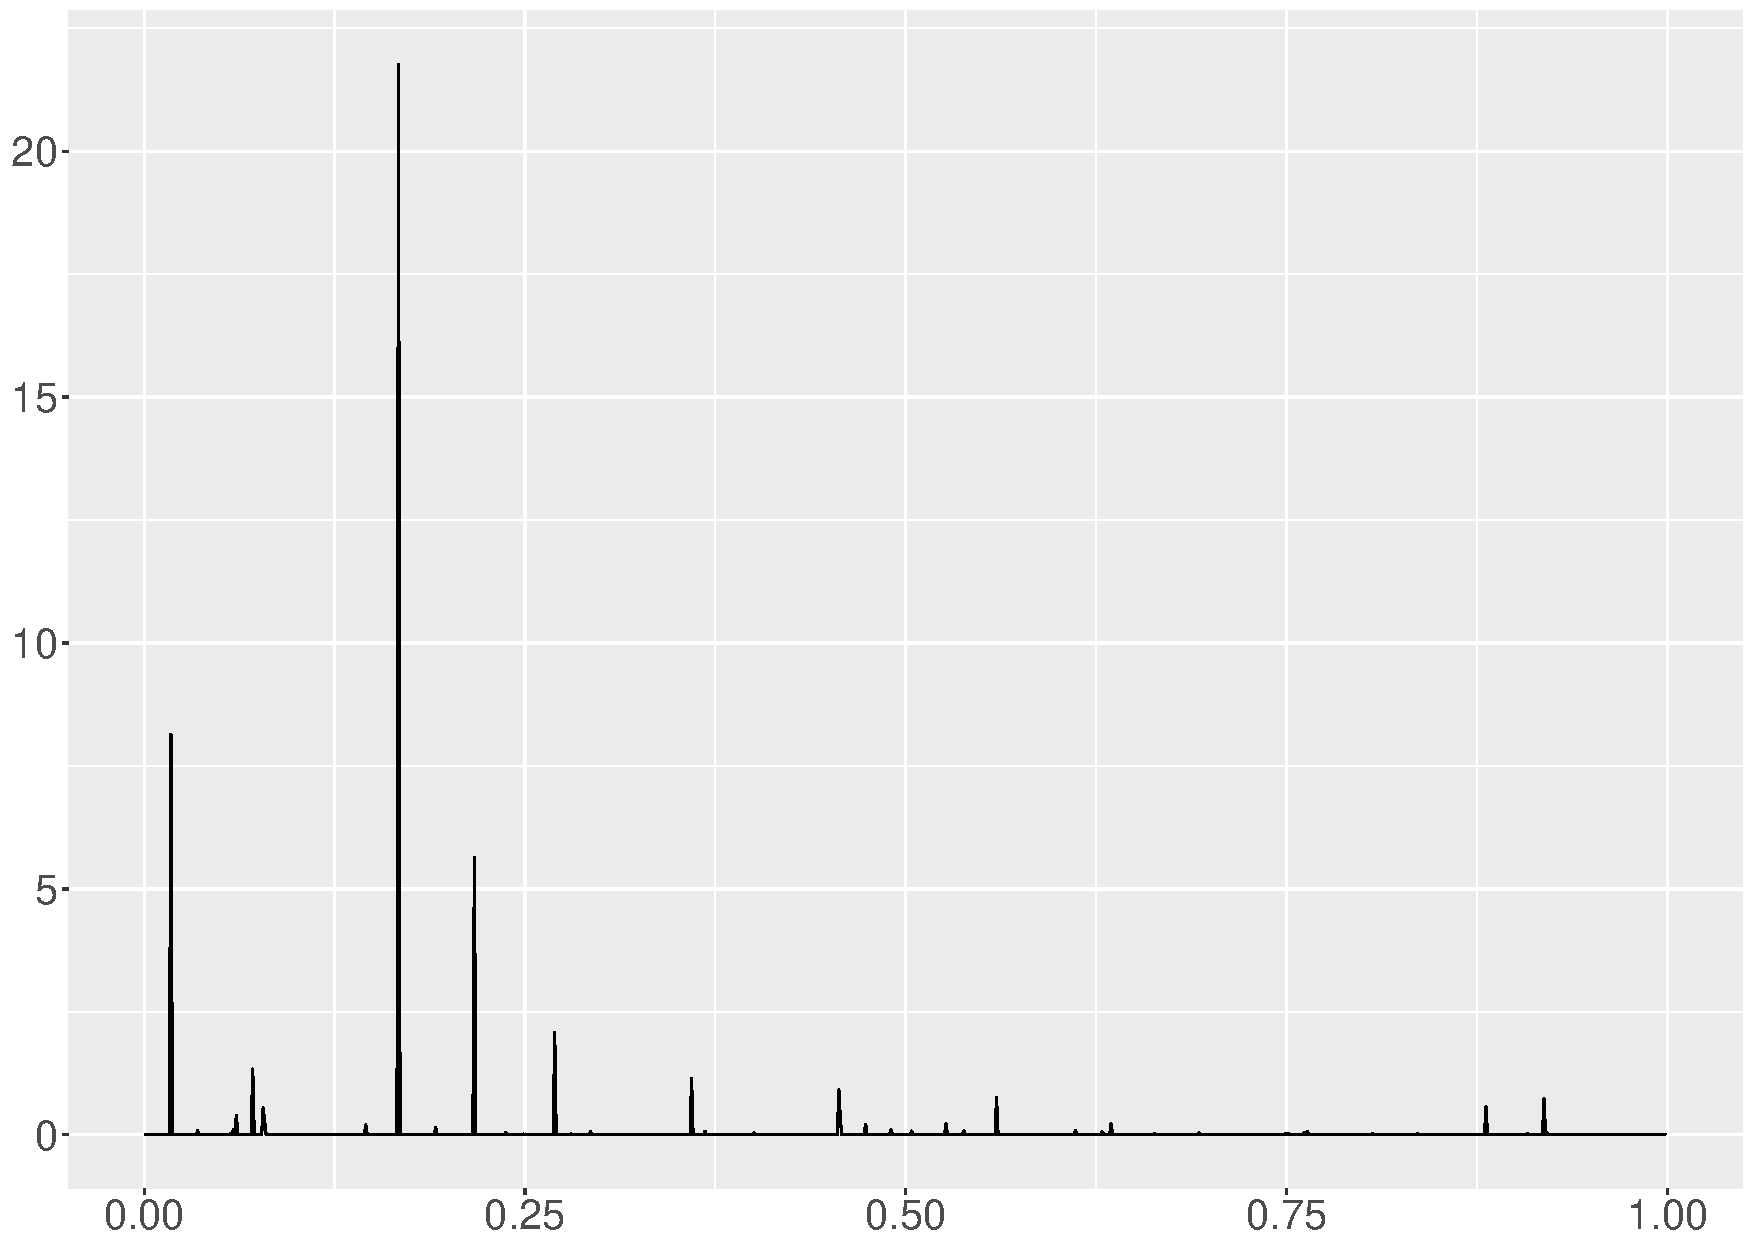
\includegraphics[width=0.45\textwidth]{Chapters/02TractorSplineTheory/plot/ggplot/ggBlocksPenaltyBar.pdf}
    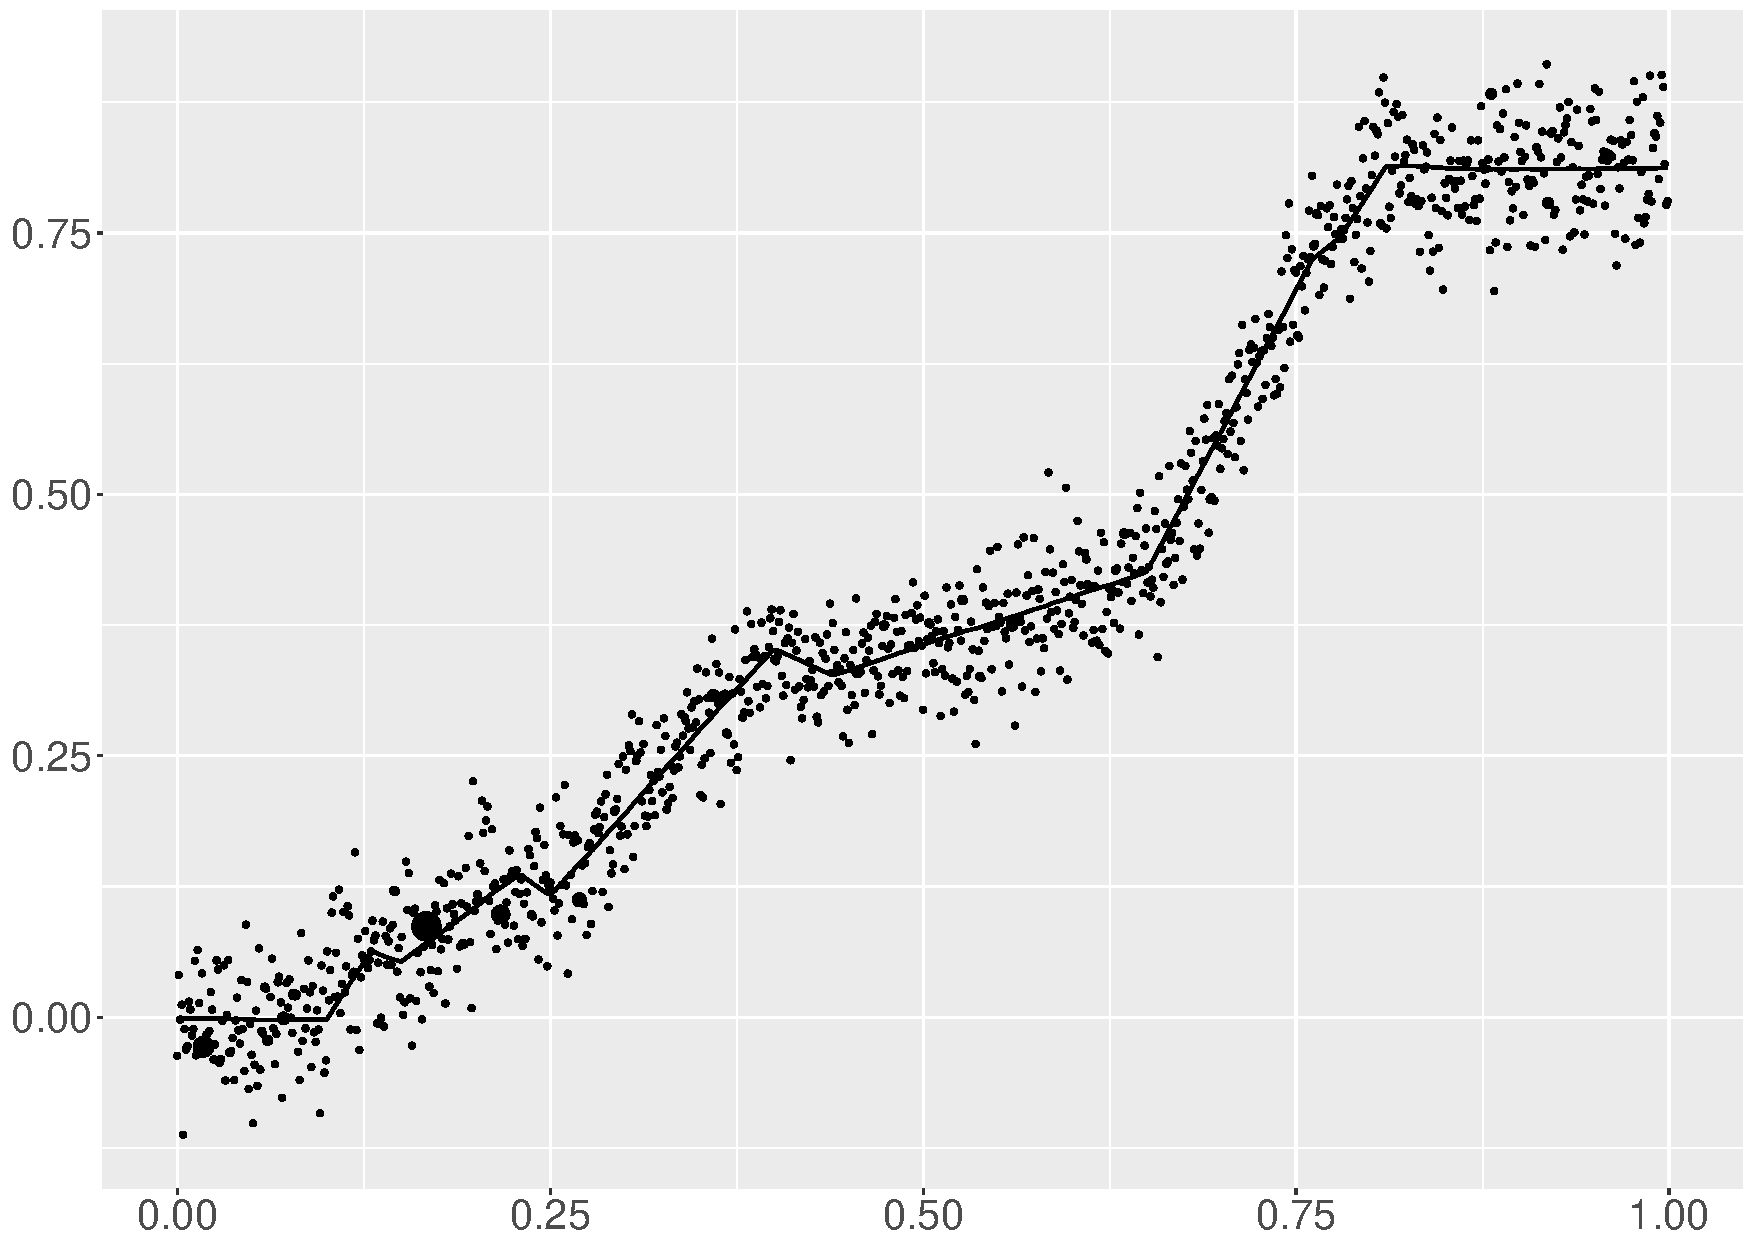
\includegraphics[width=0.45\textwidth]{Chapters/02TractorSplineTheory/plot/ggplot/ggBlocksPenaltyLine.pdf}
    \caption{Distribution of the penalty values in reconstructed \textit{Blocks}}
    \end{subfigure}
    \begin{subfigure}{\textwidth}
    \centering
    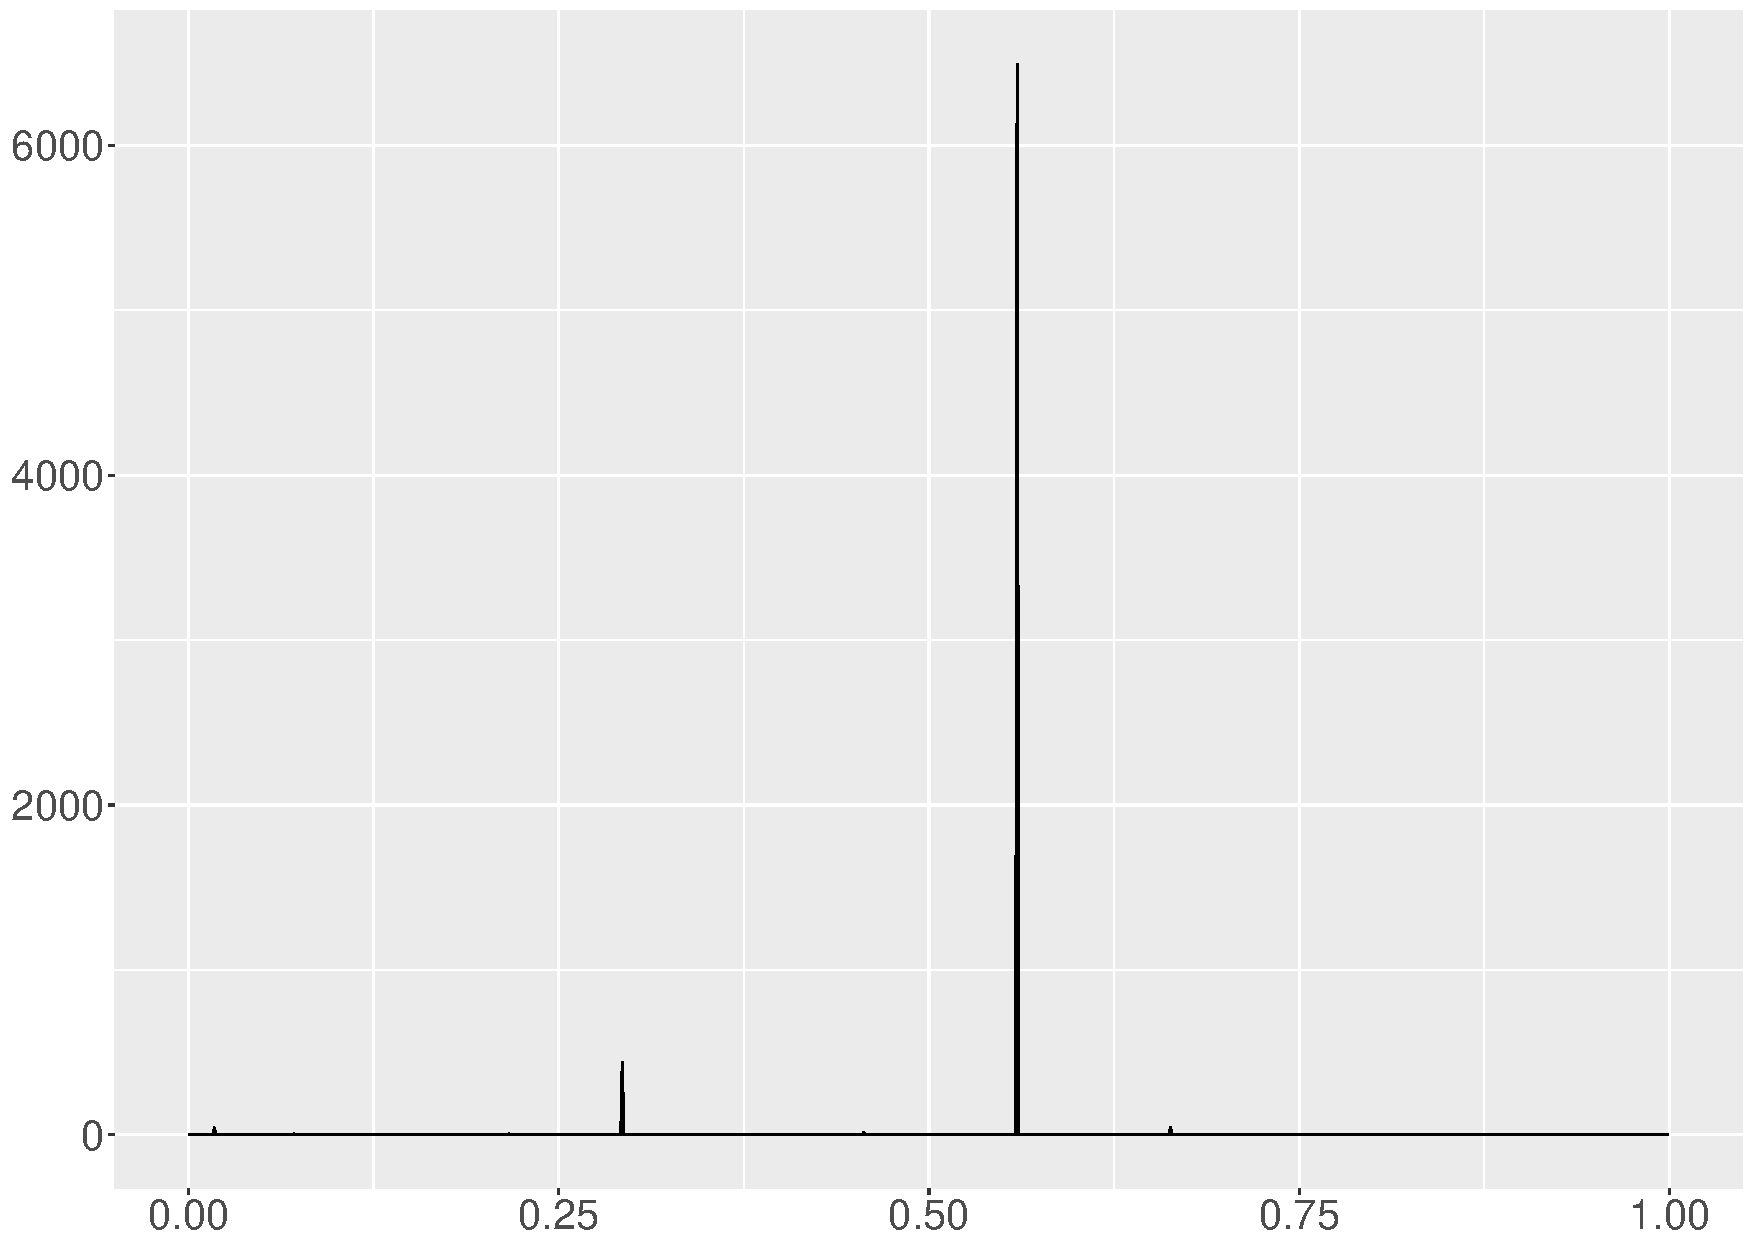
\includegraphics[width=0.45\textwidth]{Chapters/02TractorSplineTheory/plot/ggplot/ggBumpsPenaltyBar.pdf}
    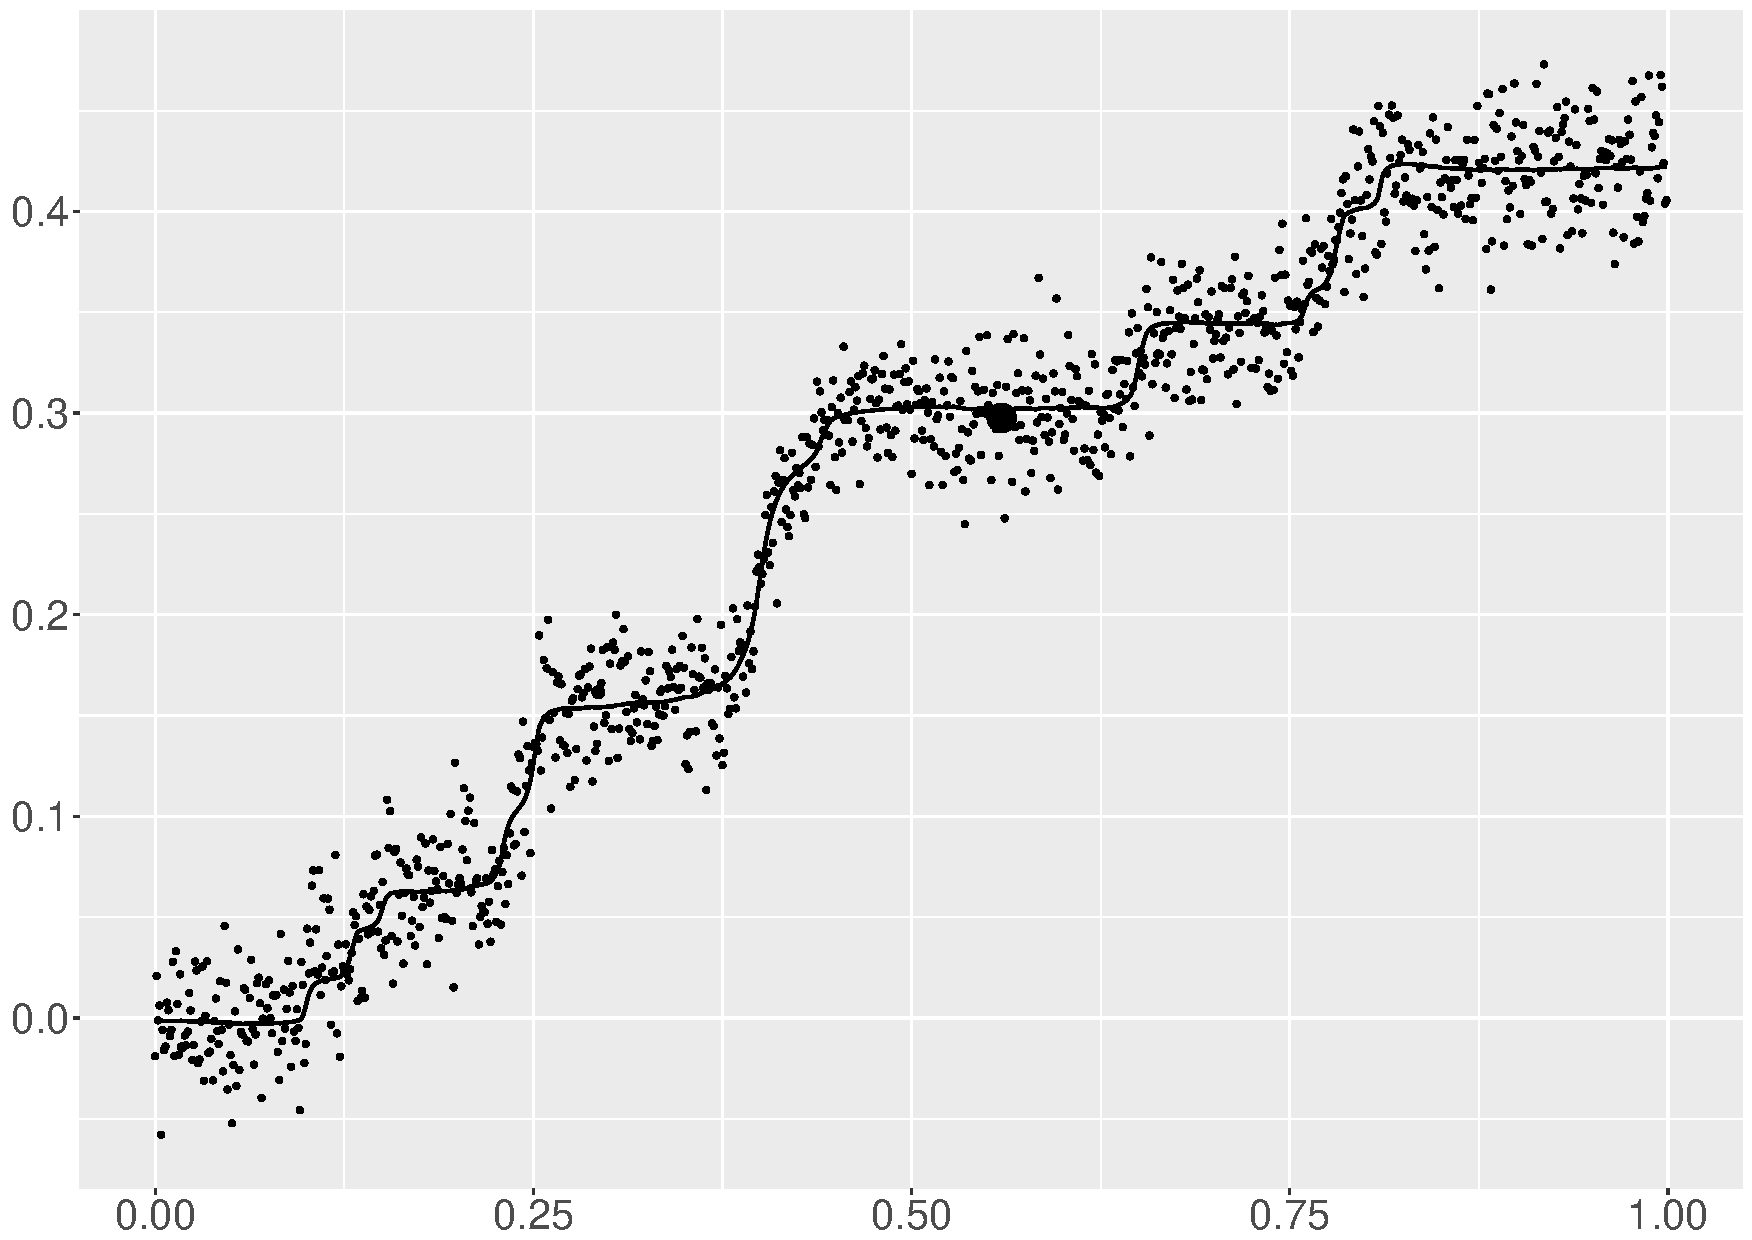
\includegraphics[width=0.45\textwidth]{Chapters/02TractorSplineTheory/plot/ggplot/ggBumpsPenaltyLine.pdf}
    \caption{Distribution of the penalty values in reconstructed \textit{Bumps}}
    \end{subfigure}
    \begin{subfigure}{\textwidth}
    \centering
    \includegraphics[width=0.45\textwidth]{Chapters/02TractorSplineTheory/plot/ggplot/ggHeaviSinePenaltyBar.pdf}
    \includegraphics[width=0.45\textwidth]{Chapters/02TractorSplineTheory/plot/ggplot/ggHeaviSinePenaltyLine.pdf}
    \caption{Distribution of the penalty values in reconstructed \textit{HeaviSine}}
    \end{subfigure}
\end{figure}
\begin{figure}\ContinuedFloat
    \centering 
    \begin{subfigure}{\textwidth}
    \centering
    \includegraphics[width=0.45\textwidth]{Chapters/02TractorSplineTheory/plot/ggplot/ggDopplerPenaltyBar.pdf}
    \includegraphics[width=0.45\textwidth]{Chapters/02TractorSplineTheory/plot/ggplot/ggDopplerPenaltyLine.pdf}
    \caption{Distribution of the penalty values in reconstructed \textit{Doppler}}
    \end{subfigure}
\caption{Distribution of the penalty values $\lambda(t)$ in V-spline. Figures on the left side indicate the values varying in intervals. On the right side, these values are projected into reconstructions. The bigger the blacks dots present, the larger the penalty values are.}\label{numpenalty}
\end{figure}


Figure \ref{numpenalty} shows the estimated penalty values $\lambda(t)=\frac{\left(\Delta t\right)^3}{\left(\Delta d\right)^2}\lambda$ at SNR=7. The figures in the left column illustrate the values of the penalty term at different intervals, the figures in the right column are the observations and reconstructed trajectory. Bigger black dots present larger penalty values. It can be seen that $\lambda(t)$ adapts to the smoothness pattern of position and will be large where a long time gap may occur. The details of how this penalty function works will be explained in next subsection. Figure \ref{TractorsplineSNR3} illustrates the reconstructions of V-spline at SNR=3.


%\begin{figure}
%\centering
%%  \begin{landscape}
%         \includegraphics[width=\textwidth,height=9cm]{Chapters/02TractorSplineTheory/plot/vtractor04} 
%%  \end{landscape}
%     \caption{Estimated velocity functions by taking the first derivative of V-spline. (a) Fitted $\textit{Blocks}$. (b) Fitted $\textit{Bumps}$. (c) Fitted $\textit{HeaviSine}$. (d) Fitted $\textit{Doppler}$.}\label{numvtractor}
%\end{figure}

\begin{figure}
    \centering
    \begin{subfigure}{0.45\textwidth}
    \centering
    \includegraphics[width=\textwidth]{Chapters/02TractorSplineTheory/plot/ggplot/ggBlocksTractorVelocity.pdf}
    \caption{Estimated \textit{Blocks}  }
    \end{subfigure}%
    \begin{subfigure}{0.45\textwidth}
    \centering
    \includegraphics[width=\textwidth]{Chapters/02TractorSplineTheory/plot/ggplot/ggBumpsTractorVelocity.pdf}
    \caption{Estimated \textit{Bumps}  }
    \end{subfigure}
    \begin{subfigure}{0.45\textwidth}
    \centering
    \includegraphics[width=\textwidth]{Chapters/02TractorSplineTheory/plot/ggplot/ggHeaviSineTractorVelocity.pdf}
    \caption{Estimated \textit{HeaviSine}  }
    \end{subfigure}
    \begin{subfigure}{0.45\textwidth}
    \centering
    \includegraphics[width=\textwidth]{Chapters/02TractorSplineTheory/plot/ggplot/ggDopplerTractorVelocity.pdf}
    \caption{Estimated \textit{Doppler}  }
    \end{subfigure}
\caption{Estimated velocity functions by V-spline. The velocity is generated from the original simulation functions by equation \eqref{generateVelocity}}\label{numvtractor}
 \end{figure}



Figure \ref{numvtractor} demonstrates the estimated velocity functions. By taking the first derivative of fitted V-spline, it is simple to get the original four velocity functions. The fittings of velocity are not as smooth as that of position, because we only care about the smoothness of position rather than velocity in our cross-validation formula \eqref{tractorcv}. However, velocity information does help us in reconstructing the trajectory.



\subsection{Evaluation}

To examine the performance of the V-spline, we conduct a evaluation by comparing the mean squared errors and true mean squared errors, which are respectively calculated with the following formulas: 
\begin{align}
\mbox{MSE}&= \frac{1}{n} \sum_{i=1}^{n} \left( y_i-\hat{f}_{\lambda,\gamma}(t_i) \right)^2,\\
\mbox{TMSE}&= \frac{1}{n} \sum_{i=1}^{n} \left( f(t_i)-\hat{f}_{\lambda,\gamma}(t_i) \right)^2.
\end{align}


%Besides the four function in previous subsection, we introduce two more functions as the author did in \citep{liu2010data}: Sin-141 and Sin-1414. The function Sin-141 is divided into three equal length intervals $B_1\oplus B_2 \oplus B_3$ on $[0,1]$ with signal generated by $sin(6\pi t)I\left\lbrace t\in (B_1,B_3)\right\rbrace + sin(24\pi t)I(t\in B_2)$, where $I(\cdot)$ is the indicator function. Sin-1414 is divided into four equal length intervals $B_1\oplus B_2 \oplus B_3 \oplus B_4$ on $[0,1]$ with signal generated by $sin(6\pi t)I\left\lbrace t\in (B_1,B_3)\right\rbrace + sin(24\pi t)I(t\in B_2,B_4)$

The results are shown in table \ref{mse3200} and \ref{tmse3200}. All of these methods have good performances in fitting noisy data. The differences of mean squared error between these methods are not significant, as can be seen from table \ref{mse3200}. The proposed method is not the best among these simulations according to MSE. However, from table \ref{tmse3200}, V-spline returns the smallest true mean squared errors. The difference is significant, that means the reconstruction from V-spline is closer to the true trajectory. 
 
%\begin{sidewaystable}
 \begin{table}
 	\centering
 	\caption{MSE. Mean squared errors of different methods. The numbers in bold indicate the least error among these methods under the same level. The difference is not significant.}\label{mse3200}
	\setlength\tabcolsep{1.5pt}
	\begin{tabular}{|c|c|C{1.9cm}|C{1.9cm}|C{1.9cm}|C{1.9cm}|C{1.9cm}|C{1.9cm}|}
\hline	MSE $\left(10^{-4}\right)$   & SNR & V-spline & VS$_{\footnotesize\gamma=0}$ & VS$_{\scriptsize \mbox{APT=0}}$   & P-spline & W(sure)& W(Bayes)\\ \hline
\multirow{2}{*}{\textit{Blocks}}     & 7   &  16.53& 15.99 & 16.69 & 16.14  & \textbf{15.39} & 16.68 \\ \cline{2-8}
       & 3   &  89.79 & \textbf{87.64} & 89.94  & 88.27 & 98.35 & 90.24 \\ \hline
\multirow{2}{*}{\textit{Bumps}}     & 7   & 4.40 & 4.19 & 4.55 & 4.33 & \textbf{4.18} & 4.59 \\ \cline{2-8}
      & 3   & 23.93 & \textbf{23.19} & 24.10 & 23.55 & 26.23 & 23.74 \\ \hline
\multirow{2}{*}{\textit{HeaviSine}}  & 7   & 4.16 & 4.01 &4.16 & 4.02 & \textbf{3.79} & 4.19 \\ \cline{2-8}
     & 3   & 22.63 & \textbf{22.19} & 22.65 & 22.02 & 23.53 & 22.07 \\ \hline
\multirow{2}{*}{\textit{Doppler}}    & 7   & 1.15 & \textbf{1.07} & 1.10 & 1.15  & \textbf{1.07} & 1.13  \\ \cline{2-8}
      & 3   & 6.27 & \textbf{5.94} &6.28 & 6.05  & 6.85 & 6.29  \\ \hline
	\end{tabular}
\end{table}
 %\end{sidewaystable}

%\begin{sidewaystable} 
\begin{table}
	\centering
	\caption{TMSE. True mean squared errors of different methods. The numbers in bold indicate the least error among these methods under the same level. The proposed V-spline returns the smallest TMSE among all the methods under the same level except for $\textit{Doppler}$ with SNR=7. The differences are significant. }\label{tmse3200}
	\setlength\tabcolsep{1.5pt}
	\begin{tabular}{|c|c|C{1.9cm}|C{1.9cm}|C{1.9cm}|C{1.9cm}|C{1.9cm}|C{1.9cm}|}
\hline	TMSE $\left(10^{-6}\right)$  & SNR & V-spline & VS$_{\footnotesize\gamma=0}$ & VS$_{\scriptsize \mbox{APT=0}}$   & P-spline & W(sure) &  W(Bayes)\\ \hline
		
\multirow{2}{*}{\textit{Blocks}}  & 7   & \textbf{1.75} & 54.25 &  28.68   & 54.76   & 201.02   & 182.12   \\ \cline{2-8}
	     & 3   & \textbf{16.44} & 152.5 & 30.76  & 171.59   & 1138.08  & 712.36  \\ \hline
\multirow{2}{*}{\textit{Bumps}}     & 7  & \textbf{1.64} & 23.44  & 21.10     & 24.21 & 71.71 & 69.26 \\ \cline{2-8}
        & 3  & \textbf{8.51} & 77.78  &37.12     & 77.52 & 330.77 & 238.79 \\ \hline
\multirow{2}{*}{\textit{HeaviSine}}  & 7 & \textbf{1.53}& 7.80  & 1.56     & 9.54   & 55.37  &44.88  \\ \cline{2-8}
      & 3 & \textbf{8.21}& 33.56  & 8.49 & 34.26 & 240.72& 110.49\\ \hline
\multirow{2}{*}{\textit{Doppler}}    & 7   & 1.51& 6.67  & \textbf{1.08}   &  8.26   & 14.87  & 12.01  \\ \cline{2-8}
    & 3   & \textbf{8.10} & 22.14  & 8.25   & 19.95    &81.48  &50.33   \\ \hline
	\end{tabular}	
\end{table}
%\end{sidewaystable}


\subsection{Residual Analysis}

The simulated data is generated by equations \eqref{tractorsplinegeneratefunctions} and the SNRs are set at 7 and 3 separately to compare the performances of different algorithms. All of the algorithms can reconstruct the true trajectory from noisy data and return acceptable MSE values, though V-spline returns the least TMSE in most of the circumstances. 

Table \ref{tablecompareSNR} is comparing the capability of V-spline in retrieving the true SNR. The measurements are generated from $f$ and $g$ with predefined SNR. The V-spline reconstructs the true trajectory and retrieves the SNR value, both of which are close to the truth. 

\begin{table}
	\centering
    \caption{Retrieved SNR. V-spline effectively retrieves the SNR, which is calculated by $\sigma_{\hat{f}} / \sigma_{(\hat{f}-y)}$. }\label{tablecompareSNR}
	\begin{tabular}{|c|C{3cm}|C{3cm}|C{3cm}|}
\hline	 SNR   & predefined value & generated $f$ & V-spline $\hat{f}$ \\ \hline
\multirow{2}{*}{\textit{Blocks}}  & 7   & 6.9442    &  6.9485     \\ \cline{2-4}
		   & 3   &  2.9761   &  2.9817   \\ \hline
\multirow{2}{*}{\textit{Bumps}}    & 7  & 6.9442    &  6.9548  \\ \cline{2-4}
		   & 3  & 2.9761    &   2.9953 	   \\ \hline
\multirow{2}{*}{\textit{HeaviSine}}  & 7 & 6.9442    &   6.9207   \\ \cline{2-4}
		  & 3 & 2.9761    &   2.9706  \\ \hline
\multirow{2}{*}{\textit{Doppler}}     & 7   & 6.9442   &  6.8757   \\ \cline{2-4}
		  & 3   & 2.9761   &  2.9625   \\ \hline
	\end{tabular}
\end{table}


%\begin{table}
%	\centering
%    \caption{Retrieved SNR. V-spline effectively retrieves the SNR, which is calculated by $\sigma_{\hat{f}} / \sigma_{(\hat{f}-y)}$. }\label{tablecompareSNR}
%\begin{tabular}{|c|c|l|c|l|c|l|} 
%\hline   & \multicolumn{2}{c|}{predefined}  & \multicolumn{2}{c|}{ from $f$ }  & \multicolumn{2}{c|}{from V-spline $\hat{f}$}  \\ \hline
%\multirow{2}{*}{blocks} & \multicolumn{2}{c|}{7} & \multicolumn{2}{c|}{7} & \multicolumn{2}{c|}{7} \\ \cline{2-7} 
%                        & \multicolumn{2}{c|}{3} & \multicolumn{2}{c|}{3} & \multicolumn{2}{c|}{3} \\ \hline
%\multirow{2}{*}{Bumps}       & \multicolumn{2}{c|}{}  & \multicolumn{2}{c|}{}  & \multicolumn{2}{c|}{}  \\ \cline{2-7} 
%                        & \multicolumn{2}{c|}{}  & \multicolumn{2}{c|}{}  & \multicolumn{2}{c|}{}  \\ \hline
%\multirow{2}{*}{HeaviSine}       & \multicolumn{2}{c|}{}  & \multicolumn{2}{c|}{}  & \multicolumn{2}{c|}{}  \\ \cline{2-7} 
%                        & \multicolumn{2}{c|}{}  & \multicolumn{2}{c|}{}  & \multicolumn{2}{c|}{}  \\ \hline
%\end{tabular}
%\end{table}

Further analysis in figures \ref{tractorsplineSNR7acf} and \ref{tractorsplineSNR3acf} shows that the residuals from V-splines are independent. 


%\clearpage 

\section{Application on Real Dataset}\label{splineapplication}

In this section, we apply the proposed V-spline to real dataset, which is recorded by a GPS unit mounted on a tractor. The original dataset contains the information about time marks, longitude, latitude, velocity, bearing (in degrees,  heading to North) and boom status. 

In a two or higher $d$-dimensional curve nonparametric regression, consider the general form of a length $n$ time series data points $\left\lbrace t_1,p_1,s_1\right\rbrace, \ldots, \left\lbrace t_n,p_n,s_n\right\rbrace$, such that $a \leq t_1<t_2< \cdots < t_n \leq b$, $p_i$ and $s_i$ are $d$-dimensional vectors contain position and velocity information at time $i$ respectively. The positive piecewise constant function $\lambda(t) = \lambda_i$ on each interval $t_i \leq t<t_{i+1}, t_0=a, t_{n+1}=b$.  Then the function $f:[a,b]\mapsto\mathbb{R}^d$ with $\gamma>0$ is a V-spline in the $d$-dimensional space if it is the solution to the generic form of the objective function: 
\begin{equation}\label{tractorsplineObjective2D}
J[f]= \frac{1}{n} \sum_{i=1}^{n} \lVert f(t_i)-p_i\rVert_d^2 + \frac{\gamma}{n} \sum_{i=1}^{n} \lVert f'(t_i)-s_i \rVert_d^2 +\sum_{i=0}^{n} \lambda_i\int_{t_i}^{t_{i+1}} \lVert f''(t)\rVert_d^2 dt. 
\end{equation}


Particularly, the GPS data is recorded in a 2-dimensional form, in which scenario $d=2$. Hence, in the following application, we split the 2-dimensional function $f(x,y)$ into two sub functions $f_x(t)$ on $x$-axis and $f_y(t)$ on $y$-axis with respect to time $t$. Compared with other parameters, choosing time $t$ to be the parameter has some advantages: (\romannum{1}) the expressions of all the constraints are simpler \citep{zhang2013cubic}; (\romannum{2}) it can be simply applied from 2-dimension to 3-dimension by adding an extra $z$-axis. Without loss of generality, a dataset in a higher dimensional space can be projected into several sub-spaces, such as $p=\left\lbrace x,y,z,\ldots \right\rbrace$ and $s=\left\lbrace u,v,w,\ldots \right\rbrace$. 


Thereafter, we convert the longitude and latitude information from a 3D sphere to 2D surface first by Universal Transverse Mercator coordinate system (UTM) and then project the speed $s$ into $u$ and $v$ on $x$-axis and $y$-axis respectively by 
\begin{align}
u &=s\cdot \sin \left(\omega\frac{\pi}{180}\right),\\
v &= s\cdot \cos \left(\omega\frac{\pi}{180}\right),
\end{align}
where $\omega$ is the bearing in degrees. Boom status is tagged as 0 if it is not operating and 1 if it is. Time marks are transformed by subtracting the first mark, in which way the time starts from 0. Time duplicated data, caused by errors, had been removed from the dataset. In the convenience of comparing with wavelet algorithm, we choose the first 512 out of 928 rows of data. The original data is plotted in figure \ref{original512}.

%\begin{figure}
%  \centering
%         \includegraphics[width=\textwidth,height=9cm]{Chapters/02TractorSplineTheory/plot/original04}
%  \caption{Original data points. (a) Original position recorded by GPS units. Circle points stand for the status of boom not operating; cross points stand for operating. (b) Original trajectory made by simply connecting GPS points sequentially. (c) Original position on $x$ axis. (d)  Original position on $y$ axis.}\label{original512}
%\end{figure}

\begin{figure}
\centering
    \begin{subfigure}{0.45\textwidth}
    \centering
    \includegraphics[width=\textwidth]{Chapters/02TractorSplineTheory/plot/ggplot/gg512Points.pdf}
    \caption{Original positions}\label{gg512Points}
    \end{subfigure}%
    \begin{subfigure}{0.45\textwidth}
    \centering
    \includegraphics[width=\textwidth]{Chapters/02TractorSplineTheory/plot/ggplot/gg512Path.pdf}
    \caption{Line-based trajectory}\label{gg512Path}
    \end{subfigure}
    \begin{subfigure}{0.45\textwidth}
    \centering
    \includegraphics[width=\textwidth]{Chapters/02TractorSplineTheory/plot/ggplot/gg512PointsX.pdf}
    \caption{Original positions on $x$-axis}\label{gg512PointsX}
    \end{subfigure}
    \begin{subfigure}{0.45\textwidth}
    \centering
    \includegraphics[width=\textwidth]{Chapters/02TractorSplineTheory/plot/ggplot/gg512PointsY.pdf}
    \caption{Original positions on $y$-axis}\label{gg512PointsY}
    \end{subfigure}
\caption{Original data points. Figure \ref{gg512Points} is th original positions recorded by GPS units. Circle points means the boom is not operating; cross points means it is operating. Figure \ref{gg512Path} is the line-based trajectory by simply connecting all points sequentially with straight lines. Figure \ref{gg512PointsX} is the original $x$ position. Figure \ref{gg512PointsY} is the original $y$ positions.}\label{original512}
 \end{figure}


To fit the real data, we bring the parameter $\lambda_d$ to our model. Then, we are now having three parameters $\lambda_d$ and $\lambda_u$ regarding boom status and $\gamma$ controlling velocity residuals. The criteria of a good fitting are that it can catch more information, recognize time gaps between two points where tractor stops and return a smaller MSE. 



\subsection{1-Dimensional Trajectory}

We treat $x$ and $y$ position separately and compare how the velocity information and the adjusted penalty term of equation \eqref{adjustedpenalty} work in our model. All parameters in fitted V-spline are automatically selected by cross-validation by equation \eqref{tractorcv}. Figure \ref{1dx} and figure \ref{1dy} compare the results of fitted methods on $x$ and $y$ axes. P-spline gives over-fitting on $x$ axis reconstruction and not applicable on $y$ axis due to errors. Wavelet(sure) misses some key points at corners when a tractor tries to turn around. V-spline without adjusted penalty term presents less fitting at time gap knots, where time marks keep increasing while position stays the same and velocity is 0. If we take the last knot $p_k$ before and the first knot $p_{k+1}$ after the time gap, Hermite spline basis will use $y_k, v_k, y_{k+1}$ and $v_{k+1}$ to build up a cubic spline, even though the velocity information is not useful. That is why we got a curve rather than a straight line. Wavelet(BayesThresh), V-spline without velocity and proposed V-spline give acceptable results.


Table \ref{1dxymse} illustrates the MSE of all methods on both $x$ and $y$ axes. The proposed V-spline returns the least errors among all methods.
%\begin{figure}
%  \centering
%   		\includegraphics[width=\textwidth,height=13cm]{Chapters/02TractorSplineTheory/plot/fittedx06}
%  \caption{Fitted data points on $x$ axis. (a) Fitted by P-spline, which gives over-fitting on these points and misses some information. (b) Fitted by wavelet ($\textit{sure}$) algorithm. At some turning points, it gives over-fitting. (c) Fitted by wavelet ($\textit{BayesThresh}$) algorithm. It fits better than ($\textit{sure}$) and the result is close to the proposed method. (d) Fitted by V-spline without velocity information. The reconstruction is good to get the original trajectory. (e) Fitted by V-spline without adjusted penalty term. It gives less fitting at boom-not-operating points because of a large time gap. (f) Fitted by proposed method. It fits all data points in a good way.}\label{1dx}
%\end{figure}
\begin{figure}
    \centering
    \begin{subfigure}{0.45\textwidth}
    \centering
    \includegraphics[width=\textwidth,height=0.5\textwidth]{Chapters/02TractorSplineTheory/plot/ggplot/ggRealdataXPSpline.pdf}
    \caption{Reconstruction by P-spline}\label{ggRealdataXPSpline}
    \end{subfigure}%
    \begin{subfigure}{0.45\textwidth}
    \centering
    \includegraphics[width=\textwidth,,height=0.5\textwidth]{Chapters/02TractorSplineTheory/plot/ggplot/ggRealdataXSure.pdf}
    \caption{Reconstruction by wavelet ($\textit{sure}$)}\label{ggRealdataXSure}
    \end{subfigure}
    \begin{subfigure}{0.45\textwidth}
    \centering
    \includegraphics[width=\textwidth,height=0.5\textwidth]{Chapters/02TractorSplineTheory/plot/ggplot/ggRealdataXBayes.pdf}
    \caption{Reconstruction by wavelet ($\textit{Bayes}$)\\ \mbox{  }}\label{ggRealdataXBayes}
    \end{subfigure}
    \begin{subfigure}{0.45\textwidth}
    \centering
    \includegraphics[width=\textwidth,height=0.5\textwidth]{Chapters/02TractorSplineTheory/plot/ggplot/ggRealdataXTractorGamma.pdf}
    \caption{Reconstruction by V-spline setting  $\gamma=0$ }\label{ggRealdataXTractorGamma}
    \end{subfigure}
    \begin{subfigure}{0.45\textwidth}
    \centering
    \includegraphics[width=\textwidth,height=0.5\textwidth]{Chapters/02TractorSplineTheory/plot/ggplot/ggRealdataXTractorAPT.pdf}
    \caption{Reconstruction by V-spline setting with conventional penalty term}\label{ggRealdataXTractorAPT}
    \end{subfigure}
    \begin{subfigure}{0.45\textwidth}
    \centering
    \includegraphics[width=\textwidth,height=0.5\textwidth]{Chapters/02TractorSplineTheory/plot/ggplot/ggRealdataXTractor.pdf}
    \caption{Reconstruction by proposed V-spline}\label{ggRealdataXTractor}
    \end{subfigure}
 \caption{Fitted data points on $x$ axis. Figure \ref{ggRealdataXPSpline} Fitted by P-spline, which gives over-fitting on these points and misses some information. Figure \ref{ggRealdataXSure} Fitted by wavelet ($\textit{sure}$) algorithm. At some turning points, it gives over-fitting. Figure \ref{ggRealdataXBayes} Fitted by wavelet ($\textit{BayesThresh}$) algorithm. It fits better than ($\textit{sure}$) and the result is close to the proposed method. Figure \ref{ggRealdataXTractorGamma} Fitted by V-spline without velocity information. The reconstruction is good to get the original trajectory. Figure \ref{ggRealdataXTractorAPT} Fitted by V-spline without adjusted penalty term. It gives less fitting at boom-not-operating points because of a large time gap. Figure \ref{ggRealdataXTractor} Fitted by proposed method. It fits all data points in a good way.}\label{1dx}
 \end{figure}



%\begin{figure}
%  \centering
%     		\includegraphics[width=\textwidth,height=13cm]{Chapters/02TractorSplineTheory/plot/fittedy06}
%  \caption{Fitted data points on $y$ axis. (a) Fitted P-spline is not applicable on $y$ axis as the matrix is not invertible. (b) Fitted by wavelet ($\textit{sure}$) algorithm. At some turning points, it gives over-fitting. (c) Fitted by wavelet ($\textit{BayesThresh}$) algorithm is much better than wavelet ($\textit{sure}$). (d) Fitted by V-spline without velocity information. The reconstruction is good to get the original trajectory. (e) Fitted by V-spline without adjusted penalty term. It gives less fitting at boom-not-operating. (f) Fitted by proposed method. It fits all data points in a good way.}\label{1dy}
%\end{figure}


\begin{figure}
    \centering
    \begin{subfigure}{0.45\textwidth}
    \centering
    \includegraphics[width=\linewidth,height=0.5\textwidth]{Chapters/02TractorSplineTheory/plot/ggplot/ggRealdataYPSpline.pdf}
    \caption{Not available for P-spline}\label{ggRealdataYPSpline}
    \end{subfigure}%
    \begin{subfigure}{0.45\textwidth}
    \centering
    \includegraphics[width=\linewidth,,height=0.5\textwidth]{Chapters/02TractorSplineTheory/plot/ggplot/ggRealdataYSure.pdf}
    \caption{Reconstruction by wavelet ($\textit{sure}$)}\label{ggRealdataYSure}
    \end{subfigure}
    \begin{subfigure}{0.45\textwidth}
    \centering
    \includegraphics[width=\linewidth,height=0.5\textwidth]{Chapters/02TractorSplineTheory/plot/ggplot/ggRealdataYBayes.pdf}
    \caption{Reconstruction by wavelet ($\textit{Bayes}$)\\ \mbox{  }}\label{ggRealdataYBayes}
    \end{subfigure}
    \begin{subfigure}{0.45\textwidth}
    \centering
    \includegraphics[width=\linewidth,height=0.5\textwidth]{Chapters/02TractorSplineTheory/plot/ggplot/ggRealdataYTractorGamma.pdf}
    \caption{Reconstruction by V-spline setting  $\gamma=0$ }\label{ggRealdataYTractorGamma}
    \end{subfigure}
    \begin{subfigure}{0.45\textwidth}
    \centering
    \includegraphics[width=\linewidth,height=0.5\textwidth]{Chapters/02TractorSplineTheory/plot/ggplot/ggRealdataYTractorAPT.pdf}
    \caption{Reconstruction by V-spline setting with conventional penalty term}\label{ggRealdataYTractorAPT}
    \end{subfigure}
    \begin{subfigure}{0.45\textwidth}
    \centering
    \includegraphics[width=\linewidth,height=0.5\textwidth]{Chapters/02TractorSplineTheory/plot/ggplot/ggRealdataYTractor.pdf}
    \caption{Reconstruction by proposed V-spline}\label{ggRealdataYTractor}
    \end{subfigure}
\caption{Fitted data points on $y$ axis. Figure \ref{ggRealdataYPSpline} Fitted P-spline is not applicable on $y$ axis as the matrix is not invertible. Figure \ref{ggRealdataYSure} Fitted by wavelet ($\textit{sure}$) algorithm. At some turning points, it gives over-fitting. Figure \ref{ggRealdataYBayes} Fitted by wavelet ($\textit{BayesThresh}$) algorithm is much better than wavelet ($\textit{sure}$). Figure \ref{ggRealdataYTractorGamma} Fitted by V-spline without velocity information. The reconstruction is good to get the original trajectory. Figure \ref{ggRealdataYTractorAPT} Fitted by V-spline without adjusted penalty term. It gives less fitting at boom-not-operating. Figure \ref{ggRealdataYTractor} Fitted by proposed method. It fits all data points in a good way.}\label{1dy}
 \end{figure}

%\begin{sidewaystable}
\begin{table}
\caption{Mean squared error. V-spline returns smallest errors among all these methods. P-spline was unable to reconstruct the $y$ trajectory as the original dataset contains 0 $\Delta_y$.} \label{1dxymse}
% \centering
	\setlength\tabcolsep{1.5pt}
\begin{center}
 	\begin{tabular}{|c|C{2cm}|C{2cm}|C{2cm}|C{2cm}|C{2cm}|C{2cm}|}
 		\hline
 		MSE   &  V-spline & VS$_{\gamma=0}$ & VS$_{\scriptsize \mbox{APT=0}}$  & P-spline &  W(sure) & W(Bayes)\\ \hline 
	\textit{$x$}   &  \textbf{0.2046} & 0.2830 & 0.3298     & 2860.5480   & 256.0494  & 6.2959  \\ \hline
	\textit{$y$}   &  \textbf{0.0020} & 0.3062 & 0.3115     & \textit{NA} & 1960.2220 & 19.3330  \\ \hline
 	\end{tabular}
 \end{center}
\end{table}
%\end{sidewaystable} 

The penalty function of the proposed V-spline is
\begin{equation}\label{penaltylamb}
\lambda(t)=b\frac{\left(\Delta t\right)^3}{\left(\Delta d\right)^2}\lambda_d+(1-b)\frac{\left(\Delta t\right)^3}{\left(\Delta d\right)^2}\lambda_u, \mbox{ where}
\begin{cases}
b=1 & \mbox{if boom is operating}\\
b=0 & \mbox{if boom is not operating}
\end{cases}
\end{equation}
To tell the differences more clearly, we take $\lambda(t)$ in our demonstration. Figure \ref{penaltyxygg} indicates that at turning points and long time gap knots, the adjusted penalty term will lead $\lambda(t)$ to large values, which forces the spline to be a straight line between two knots. It can be seen in figure \ref{penaltyxyggXYPath} clearly. Histogram plots of $\lambda(t)$ show that most of the penalty values are small, which allows the V-spline to go as closer as possible to the observed points. Only a few of penalty values are large, so that V-spline gives a straight line at tricky points. 

%\begin{figure}
%  \centering
%    \includegraphics[width=\textwidth,height=13cm]{Chapters/02TractorSplineTheory/plot/penaltyxy06} 
%  \caption{Penalty function of V-spline on $x$ and $y$ axes. The big black dots in plots (c) and (d) represent large penalty function.}\label{penaltyxygg}
%\end{figure}

\begin{figure}
    \centering
    \begin{subfigure}{\textwidth}
    \centering
    \includegraphics[width=0.45\linewidth]{Chapters/02TractorSplineTheory/plot/ggplot/ggRealdataXPenaltyLine2.pdf}
    \includegraphics[width=0.45\linewidth]{Chapters/02TractorSplineTheory/plot/ggplot/ggRealdataYPenaltyLine2.pdf}
    \caption{Distribution of the penalty term on $x$ and $y$}\label{penaltyxyggXYLine}
    \end{subfigure}
%    \begin{subfigure}{\textwidth}
%    \centering
%    \includegraphics[width=0.45\linewidth]{Chapters/02TractorSplineTheory/plot/ggplot/ggRealdataXPenaltyHist.pdf}
%    \includegraphics[width=0.45\linewidth]{Chapters/02TractorSplineTheory/plot/ggplot/ggRealdataYPenaltyHist.pdf}
%    \caption{Histograms of the penalty term on $x$ and $y$}\label{penaltyxyggXYHist}
%    \end{subfigure}
    \begin{subfigure}{\textwidth}
    \centering
    \includegraphics[width=0.45\linewidth]{Chapters/02TractorSplineTheory/plot/ggplot/ggRealdataXPenaltyPath2.pdf}
    \includegraphics[width=0.45\linewidth]{Chapters/02TractorSplineTheory/plot/ggplot/ggRealdataYPenaltyPath2.pdf}
    \caption{Reconstruction on $x$ and $y$}\label{penaltyxyggXYPath}
    \end{subfigure}
 %\caption{The penalty term $n\theta^\top\Omega\theta$ of V-spline on $x$ and $y$ axes. The big black dots in figure \ref{penaltyxyggXYPath} indicate large penalty values. It can be seen that most of large penalty values occur at turnings, where the tractor likely slows down and takes breaks. }\label{penaltyxygg}
 \caption{The penalty value $\lambda(t)$ of the V-spline on $x$ and $y$ axes. Red dots are the measurements $\mathbf{y}$. The bigger red dots in figure \ref{penaltyxyggXYPath} indicate larger penalty values. It can be seen that most of large penalty values occur at turnings, where the tractor likely slows down and takes breaks. }\label{penaltyxygg}
 \end{figure}

The 1-dimensional reconstruction gets the best fittings $\hat{f}_x$ and $\hat{f}_y$ on $x$ and $y$ axes separately using different penalty values, denoted as $\lambda_{d,x}$, $\lambda_{u,x}$, $\lambda_{d,y}$, $\lambda_{u,y}$, $\gamma_x$ and $\gamma_y$. The final reconstruction is the combination of  $\hat{f}_x$ and $\hat{f}_y$. It is shown in figure \ref{1DCombinedXY}. 
\begin{figure}
  \centering
    \includegraphics[width=\textwidth,height=10cm]{Chapters/02TractorSplineTheory/plot/ggplot/ggRealdataCombinedXY2.pdf} 
  \caption{Combined reconstruction on $x$ and $y$. Red dots are the measurements $\mathbf{y}$. The bigger size it is, the larger penalty value it indicates. }\label{1DCombinedXY}
\end{figure}



\subsection{2-Dimensional Trajectory}

In a 2-dimensional trajectory reconstruction, different from combined 1-dimensional reconstruction, we use the same parameters $\lambda_d$, $\lambda_u$ and $\gamma$ for both $x$ and $y$ axes. The overall best parameters return the least cross-validation score on all axes. Explicitly, it is calculated by the following formula 
\begin{equation}
\mbox{CV}=\mbox{CV}_x+\mbox{CV}_y.
\end{equation}
In the adjusted penalty term, $\Delta d$ is the Euclidean distance $\Delta_d(p_1,p_2)=\sqrt{(\Delta x)^2+(\Delta y)^2}$ between two positions on the 2D surface. Similarly in 1-dimensional reconstruction, the velocity information keeps trajectory in the right direction and the penalty term makes sure that the crazy curve will disappear between long-time-gap points. Figure \ref{completecombind2dxy} demonstrates the complete 2D reconstruction of the whole dataset.  
%fitted trajectory on $x$ and $y$ axes separately and compares the final 2D trajectory with the line based original one. 
%\begin{figure}
%  \centering
%    \includegraphics[width=\textwidth,height=9cm]{Chapters/02TractorSplineTheory/plot/fittedoriginal04} 
%  \caption{Fitted data points on $x$ and $y$ axes. The mean squared errors (MSE) on $x$ and $y$ are 0.240734 and 0.478422 respectively. The mean distance error $\sqrt{(\hat{f}_x-x)^2+ (\hat{f}_y-y)^2}$ is 0.645830.}\label{2dxy}
%\end{figure}
\begin{figure}
  \centering
 \begin{subfigure}{\textwidth}
     \centering
%     \includegraphics[width=0.45\linewidth]{Chapters/02TractorSplineTheory/plot/ggplot/ggRealdataXYPenaltyPathofX.pdf}
%     \includegraphics[width=0.45\linewidth]{Chapters/02TractorSplineTheory/plot/ggplot/ggRealdataXYPenaltyPathofY.pdf}
     \includegraphics[width=0.45\linewidth]{Chapters/02TractorSplineTheory/plot/ggplot/ggRealdataXYPenaltyPathofX2.pdf}
     \includegraphics[width=0.45\linewidth]{Chapters/02TractorSplineTheory/plot/ggplot/ggRealdataXYPenaltyPathofY2.pdf}
     \caption{2-dimensional reconstruction on separate $x$ and $y$}
     \end{subfigure}
     \begin{subfigure}{\textwidth}
     \centering
     \includegraphics[width=0.9\linewidth]{Chapters/02TractorSplineTheory/plot/ggplot/ggRealdataXYPenaltyPathofXY2.pdf}
     \caption{2-dimensional reconstruction}
     \end{subfigure}
%\includegraphics[width=\textwidth,height=10cm]{Chapters/02TractorSplineTheory/plot/ggplot/ggRealdataXYPenaltyPath.pdf} 
 %\caption{2-Dimensional reconstruction with penalty function. Larger dots indicate bigger penalty values. The mean squared errors (MSE) on $x$ and $y$ are 0.2407 and 0.4784 respectively. The mean distance error $\sqrt{(\hat{f}_x-x)^2+ (\hat{f}_y-y)^2}$ is 0.6458.}\label{2dxy}
 \caption{2-dimensional reconstruction. Larger dots indicate bigger values of penalty function $\lambda(t)$.}\label{completecombind2dxy}
\end{figure}

%The penalty term of a 2-dimension reconstruction will be the sum of each penalty on $x$ and $y$ axes. So the estimated penalty function is
%\begin{equation}
%\lambda(t)=\lambda(t)_x+\lambda(t)_y
%\end{equation}
%and presented in figure \ref{2dpenalty}. As the similar results in 1 dimension reconstruction, most of large penalty values appear in long time gap knots and turning points. A histogram plot of penalty function shows that most of the values are small and only a couple of them are large. 
%\begin{figure}
%  \centering
%    \includegraphics[width=\textwidth,height=9cm]{Chapters/02TractorSplineTheory/plot/penaltyoriginal04} 
%  \caption{Penalty function of 2 dimensional reconstruction. Bigger black dots present larger penalty value on $x$ and $y$ axes simultaneously.}\label{2dpenalty}
%\end{figure}
The penalty function $\lambda(t)$ of a 2-dimensional reconstruction is shared by $x$ and $y$ axes and presented in figure \ref{2dpenalty}. The complete penalty term is 
\begin{equation*}
n\theta_x^\top\Omega_{\lambda_d,\lambda_u}\theta_x + n\theta_y^\top\Omega_{\lambda_d,\lambda_u}\theta_y.
\end{equation*}
Similarly, most of the large penalty values appear at long-time-gap knots and turning points. A histogram plot of penalty function shows that most of the values are small and only a couple of them are large. 
\begin{figure}
  \centering
    \includegraphics[width=0.45\textwidth]{Chapters/02TractorSplineTheory/plot/ggplot/ggRealdataXYPenaltyLine.pdf}
    \includegraphics[width=0.45\textwidth]{Chapters/02TractorSplineTheory/plot/ggplot/ggRealdataXYPenaltyHist.pdf} 
  \caption{Penalty value of $\lambda(t)$ in 2-dimensional reconstruction.}\label{2dpenalty}
\end{figure}


The following figure \ref{complete2DXY} is a complete reconstruction from the whole observed dataset $\left\lbrace x,u,y,v\right\rbrace$. The overall reconstruction gives a smoothing path that goes through each measurement and avoids curvatures at turning points. 
%Instead of reconstructing on $x$ and $y$ axes separately, it chooses the penalty value with respect to the balance on both of the two directions. 
\begin{figure}
\centering
\includegraphics[width=0.9\linewidth]{Chapters/02TractorSplineTheory/plot/ggplot/ggRealdataCompleteXY.pdf}
\caption{2-dimensional reconstruction. Larger dots indicate bigger values of penalty function $\lambda(t)$.}\label{complete2DXY}
\end{figure}


%\clearpage

\section{Conclusion and Discussion}

In this chapter, a V-spline model is proposed to solve the objective function, which is consisting of both position and velocity information. The adjusted penalty function adapts to complicated curvatures. In a high $d$-dimensional space, V-spline can be projected into sub-spaces with respect to $t$ and combined each solution together as a final. This method performs better when we know $p$ and $s$ information than other methods. 

Additionally, the reconstruction of a V-spline contains $4\times (n-1)$ parameters if we have $n$ knots. By adding $2\times (n-2)$ constraints, the original function, and its first derivative are continuous at each interior knots, the degrees of freedom will be $4\times (n-1)-2\times (n-2)=2n$. Because there are $n$ position and $n$ velocity points, thus we do not need to specify more parameters or add more constraints to the model. 

Even though the mean squared errors of a V-spline is not the least comparing with other methods, the true mean squared errors are the least of among all the methods. That means the reconstruction is closer to the true path. 

In parameter selection, the cross-validation only focuses on the errors of $f$ ignoring that in $f'$. So the reconstruction of $f'$ is not as smooth as that of $f$, which does not affect trajectory reconstruction. A drawback of V-spline is that the computing time in finding local minimal CV score is higher than using B-spline. If there is an efficient way to compute matrix inverse, the calculation speed will be much faster. So in the simulation and application studies, we try to optimize our coding to make it run as faster as possible.

Another potential application of V-spline is to vessel monitoring system. The system is a fisheries surveillance that allows environmental and fisheries regulatory organization to track and monitor the activities of fishing vessels. The system calculates the position of the moving object and sends a data report to shore-side users. This information includes time, latitude and longitude positions. However, due to weak signals, the tracking system may lose useful information. The V-spline can help to reconstruct the whole trajectory for a fishery vessel and to analyze its behavior. For example, a larger penalty value indicates stops on the sea inferring that the vessel is casting nets; a smaller penalty value indicates the vessel is moving normally. 

After all, there is a wide range of applications for V-spline in real life. A future work is to implement V-spline on-line for instant estimation and to make it run faster. 


\clearemptydoublepage

\chapter{Tractor Spline as Bayes Estimate}\label{ChapterGPR}


\section{Introduction}

A Hilbert space is a real or complex inner product space with respect to the distance function induced by the inner product \citep{dieudonne2013foundations}. In particular, the Hilbert space $\mathcal{L}_2[0,1]$ is the set of square integrable functions $f(t):[0,1]\mapsto \mathbb{R}$, where all functions satisfy 
\begin{equation*}
\mathcal{L}_2[0,1] =\left\lbrace f:\int_0^1f^2dt <\infty \right\rbrace
\end{equation*}
with an inner product $\langle f,g\rangle=\int_0^1fgdt$. 

Consider a regression problem with observations modeled as $y_i = f(t_i)+\varepsilon_i$, $i=1,\ldots,n$, where $\varepsilon_i\sim N(0,\sigma^2)$ are \iid Gaussian noise and $f\in\mathcal{C}^{(m)}[0,1]=\{f:f^{(m)}\in \mathit{L}_2[0,1]\}$. The classic nonparametric or semi-parametric regression is a function that minimizes the following penalized sum of squares functional 
\begin{equation}\label{GaussianProcessGeneralObjective}
\frac{1}{n}\sum_{i=1}^{n}\left( y_i-f(t_i) \right)^2 + \lambda \int_{0}^{1} \left( f^{(m)}\right)^2dt, 
\end{equation}
where the first term is the lack of fit of $f$ to the data. The parameter $\lambda$ in the second term is a fixed smoothing parameter controlling the trade-off between over-fitting and bias \citep{esl2009}. The minimizer $f_\lambda$ of the above equation resides in an $n$-dimensional space and the computation in multivariate settings is generally of the order $\BigO{n^3}$ \citep{kim2004smoothing}. \cite{schoenberg1964spline} shows that a piecewise polynomial smoothing spline of degree $2m-1$ provides an aesthetically satisfying method for estimating $f$ if $\mathbf{y}$ cannot be interpolated exactly by some polynomial of degree less than $m$. For instance, when $m=2$, a piecewise cubic smoothing spline provides a powerful tool to estimate the above nonparametric function, in which the penalty term is $\int f''^2dt$ \citep{hastie1990generalized}. 


Further, \cite{wahba1978improper} shows that a Bayesian version of this problem is to take a Gaussian process prior $f(t_i) = a_0+a_1t_i+\cdots + a_{m-1}t_i^{m-1} + x_i$ on $f$ with $x_i=X(t_i)$ being a zero-mean Gaussian process whose $m$th derivative is scaled white noise, $i=1,\ldots,n$ \citep{speckman2003fully}. The extended Bayes estimates $f_\lambda$ with a ``partially diffuse'' prior is exactly the same as the spline solution. \cite{heckman1991minimax} show that if prior distribution of the vector  $\mathbf{f}=(f(t_1),\ldots,f(t_n))^\top$ is unknown but lies in a known class $\Omega$,
the estimator $\hat{f}$ is found by minimizing the $\max\E\lbrack \hat{f}-f\rbrack^2$. \cite{branson2017nonparametric} propose a Gaussian process regression method that acts as a Bayesian analog to local linear regression for sharp regression discontinuity designs. It is no doubt that one of the attractive features of the Bayesian approach is that, in principle, one can solve virtually any statistical decision or inference problem. Particularly, one can provide an accuracy assessment for $\hat{f}=\E (f\mid \mathbf{y})$ using posterior probability regions \citep{cox1993analysis}. 


Based on the correspondence between nonparametric regression and Bayesian estimation, \cite{craven1978smoothing} propose an generalized cross-validation estimate for the minimizer $f_\lambda$. The estimate $\hat{\lambda}$ is the minimizer of the function where the trace of matrix $A(\lambda)$ in \eqref{crossvalidationmatrixA} is incorporated. It is also possible to establish an optimal convergence property for the estimator when the number of observations in a fixed interval tends to infinity \citep{wecker1983signal}. A highly efficient algorithm to optimize generalized cross-validation and generalized maximum likelihood scores with multiple smoothing parameters via the Newton method was proposed by \cite{gu1991minimizing}. This algorithm can also be applied to maximum likelihood estimation and restricted maximum likelihood estimation. The behavior of the optimal regularization parameter in different regularization methods was investigated by \cite{wahba1990optimal}. 


In this chapter, it is proved that the V-spline can be estimated by a Bayesian approach in a certain reproducing kernel Hilbert space. An extended GCV is used to find the optimal parameters for the V-spline. 



\section{Polynomial Smoothing Splines on $[0, 1]$ as Bayes Estimates}

A polynomial smoothing spline of degree $2m-1$ is a piecewise polynomial of the same degree on each interval $[t_i,t_{i+1})$, $i=1, \ldots, n-1$, and the first $2m-2$ derivatives are continuous at the knots. For instance, when $m=2$,  a piecewise cubic smoothing spline is a special case of the polynomial smoothing spline providing a powerful tool to estimate the above nonparametric function \eqref{GaussianProcessGeneralObjective} in the space  $\mathcal{C}^{(2)}[0,1]$, where the penalty term is $\int f''^2dt$ \citep{hastie1990generalized, wang1998smoothing}. If a general space $\mathcal{C}^{(m)}[0,1]$ is equipped with an appropriate inner product, it can be made into a reproducing kernel Hilbert space. 

\subsection{Polynomial Smoothing Spline}

A spline is a numeric function that is piecewise-defined by polynomial functions, and which possesses a high degree of smoothness at the places where the polynomial pieces connect (known as knots) \citep{judd1998numerical, chen2009feedback}. Suppose we are given observed data $(t_1,y_1),(t_2,y_2), \ldots, (t_n,y_n)$ in the interval $[0,1]$, satisfying $0< t_1< t_2 < \cdots <t_n < 1$, a piecewise polynomial function $f(t)$ can be obtained by dividing the interval into contiguous intervals $(t_1,t_2),\ldots,(t_{n-1},t_n)$ and represented by a separate polynomial on each interval. For any continuous $f\in \mathcal{C}^{(m)}[0,1]$, it can be represented in a linear combination of basis functions $h_m(t)$ as $f(t) =\sum_{m=1}^{M}\beta_mh_m(t)$, where $\beta_m$ are coefficients \citep{ellis2009}. It is just like every vector in a vector space can be represented as a linear combination of basis vectors. 



A smoothing polynomial spline is uniquely the smoothest function that achieves a given degree of fidelity to a particular data set \citep{whittaker1922new}. In deed, the minimizer of function \eqref{GaussianProcessGeneralObjective} is the curve estimate $\hat{f}(t)$ over all spline functions $f(t)$ with $m-1$ continuous derivatives fitting observed data in the space $\mathcal{C}^{(m)}[0,1]$. In fact, \cite{kimeldorf1971some, kimeldorf1970correspondence}  prove that the minimizer $f_\lambda$ of function \eqref{GaussianProcessGeneralObjective} has the following form 
\begin{equation}\label{gausspriorequation}
f(t)=\sum_{\nu=1}^m d_\nu \phi_\nu(t)+\sum_{i=1}^n c_iR_1(t,t_i).
\end{equation}
%where $\phi_\nu (t)=\frac{t^{\nu-1}}{(\nu-1)!}$, $\nu=1, \ldots, m$. 
where $\left\lbrace \phi_\nu(t)\right\rbrace$ is a set of basis functions of space $\mathcal{H}_0$ and $R(\cdot,\cdot)$ is the reproducing kernel in $\mathcal{H}_1$. 

Additionally, the coefficients $c_i$ and $d_\nu$ might be changed when different $\phi_\nu$ and $R_1$ are used, but the function estimate remains the same regardless of the choices of $\phi_\nu$ and $R_1$ \citep{gu2013smoothing}.


\subsection{Reproducing Kernel Hilbert Space on $[0,1]$}

For any $f\in \mathcal{C}^{(m)}[0,1]$, its standard Taylor expansion is  
\begin{equation}
f(t) = \sum_{\nu=0}^{m-1}\frac{t^\nu}{\nu!}f^{(\nu)}(0) + \int_{0}^{1}\frac{(t-u)_+^{m-1}}{(m-1)!}f^{(m)}(t)dt,
\end{equation}
where $(\cdot)_+ =\max(0, \cdot)$. With an inner product 
\begin{equation}
\langle f,g \rangle = \sum_{\nu=0}^{m-1}f^{(\nu)}(0)g^{(\nu)}(0) +  \int_{0}^{1}f^{(m)}(t) g^{(m)}(t)dt,
\end{equation}
the representer is 
\begin{equation}\label{GaussianProcessKernelR}
R_s(t) =\sum_{\nu=0}^{m-1} \frac{s^{\nu}}{\nu!} \frac{t^{\nu}}{\nu!} +\int_0^1\frac{ (s-u)_+^{m-1}}{(m-1)!} \frac{ (t-u)_+^{m-1}}{(m-1)!} du \triangleq R_0(s,t)+R_1(s,t). 
\end{equation}
It is easy to prove that $R(s,t)$ is non-negative and is reproducing kernel, by which $\langle R(s,t),f(t) \rangle = \langle R_s(t),f(t) \rangle=f(s)$. Additionally, $R_s^{(\nu)}(0) = s^\nu/\nu!$ for $\nu = 0,\ldots, m-1$.

Before moving on to further steps, we are now introducing the following two theorems. 
\begin{theorem}\citep{aronszajn1950theory}\label{theoremRKHS}
Suppose $R$ is a symmetric, positive definite kernel on a set $X$. Then, there is a unique Hilbert space of functions on $X$ for which $R$ is a reproducing kernel. 
\end{theorem}
\begin{theorem}\citep{gu2013smoothing}\label{theoremKernel}
If the reproducing kernel $R$ of a space $\mathcal{H}$ on domain $X$ can
be decomposed into $R = R_0 + R_1$, where $R_0$ and $R_1$ are both non-negative definite, $R_0(x, \cdot),R1(x,\cdot) \in \mathcal{H}$, for $ \forall x \in X$, and $\langle R_0(x, \cdot),R_1(y, \cdot) \rangle= 0$, for $\forall x, y \in X$, then the spaces $\mathcal{H}_0$ and $\mathcal{H}_1$ corresponding respectively to $R_0$ and $R_1$ form a tensor sum decomposition of $\mathcal{H}$. Conversely, if $R_0$ and $R_1$ are both  nonnegative definite and $\mathcal{H}_0 \cap \mathcal{H}_1 =\left\lbrace 0\right\rbrace$, then $\mathcal{H} =\mathcal{H}_0 \oplus \mathcal{H}_1$ has a reproducing kernel $R = R_0 + R_1$.
\end{theorem}

According to Theorem \ref{theoremRKHS}, the Hilbert space associated with $R(\cdot)$ can be constructed as containing all finite linear combinations of the form $\sum a_iR(t_i,\cdot)$, and their limits under the norm induced by the inner product $\langle R(s,\cdot),R(t,\cdot) \rangle = R(s,t)$. As for Theorem \ref{theoremKernel}, it is easy to verify that $R_0$ corresponds to the space of polynomials $\mathcal{H}_0 =\left\lbrace f:f^{(m)}=0\right\rbrace$ with an inner product $\langle f, g \rangle_0 = \sum_{\nu=0}^{m-1} f^{(\nu)}(0)g^{(\nu)}(0)$ and $R_1$ corresponds to the orthogonal complement of $\mathcal{H}_0$, that is $\mathcal{H}_1 =\left\lbrace   f:f^{(\nu)}(0)=0,\nu = 0, \ldots,m-1, \int_{0}^{1}(f^{(m)})^2dt <\infty  \right\rbrace$ with an inner product $\langle f, g\rangle_1 = \int_{0}^{1}f^{(m)}g^{(m)}dt $. 



\subsection{Polynomial Smoothing Splines as Bayes Estimates}

Because it is possible to interpret the smoothing spline regression estimator as a Bayes estimate when the mean function $r(\cdot)$ is given an improper prior distribution \citep{wahba1990spline, berlinet2011reproducing}. Therefore, one can find that the posterior mean of $f$ on $[0,1]$ with a vague improper prior is the polynomial smoothing spline of the objective function  \eqref{GaussianProcessGeneralObjective}. 

Consider $f=f_0+f_1$ on $[0,1]$, with $f_0$ and $f_1$ having independent Gaussian priors with zero means and covariances satisfying  
\begin{align}
\E \lbrack f_0(s)f_0(t)\rbrack  &= \tau^2 R_0(s,t)=\tau^2 \sum_{\nu=0}^{m-1}\frac{s^\nu}{\nu!}\frac{t^\nu}{\nu!},\label{Ef0f0} \\
\E \lbrack f_1(s)f_1(t) \rbrack &= bR_1(s,t) = b\int_{0}^{1} \frac{(s-u)_+^{m-1}}{(m-1)!} \frac{(t-u)_+^{m-1}}{(m-1)!},\label{Ef1f1}
\end{align}
where $R_0$ and $R_1$ are from \eqref{GaussianProcessKernelR}. Because of the observations are normally distributed as $y_i\sim N(f(t_i),\sigma^2)$, then the joint distribution for $\mathbf{y} = \left\lbrace y_1,\ldots,y_n\right\rbrace$ and $f(t)$ is normal with zero mean and the following covariance matrix 
\begin{align*}\Cov (f,\mathbf{y}) = 
\begin{bmatrix}
bQ+\tau SS^\top+\sigma^2 I & b\xi +\tau^2 S\phi \\
b\xi^\top + \tau^2\phi^\top S^\top & bR_1(t,t) +\tau^2\phi^\top \phi
\end{bmatrix},
\end{align*}
where $\left\lbrace Q_{i,j}\right\rbrace_{n\times n}=R_1(t_i,t_j)$, $\left\lbrace S_{i,\nu}\right\rbrace_{n\times m}=t_i^{\nu-1}/(\nu-1)!$, $\left\lbrace \xi_{i,1}\right\rbrace_{n\times 1}=R_1(t_i,t)$ and $\left\lbrace \phi_{\nu,1}\right\rbrace_{m\times 1}=t^{\nu-1}/(\nu-1)!$. 
Consequently, the posterior is 
\begin{equation}
\begin{split}
\E \lbrack f(t)\mid\mathbf{y}\rbrack &= \left(b\xi^\top +\tau \phi^\top s^\top\right)\left(bQ+\tau^2 SS^\top+\sigma^2I\right)^{-1}\mathbf{y} \\
&= \xi^\top\left(Q+\rho SS^\top+n\lambda I\right)^{-1}\mathbf{y}+ \phi^\top\rho S^\top\left(Q+\rho SS^\top +n\lambda I\right)^{-1}\mathbf{y},
\end{split}
\end{equation}
where $\rho = \tau^2/b$ and $n\lambda=\sigma^2/b$. Furthermore, by denoting $M=Q+n\lambda I$, \cite{gu2013smoothing} gives that, when $\rho\rightarrow \infty$, the posterior mean is in the form $\E\lbrack f(t)\mid y_{1:n}\rbrack = \xi^\top\mathbf{c}+\phi^\top\mathbf{d}$ with coefficients
\begin{align}
\mathbf{c}&=\left(M^{-1}-M^{-1}S\left(S^\top M^{-1}S\right)^{-1}S^\top M^{-1}\right)\mathbf{y},\\
\mathbf{d}&=\left(S^\top M^{-1}S\right)^{-1}S^\top M^{-1}\mathbf{y}.
\end{align}

\begin{theorem}\citep{gu2013smoothing}
The polynomial smoothing spline of \eqref{GaussianProcessGeneralObjective} is the posterior mean of $f = f_0 +f_1$, where $f_0$ diffuses in span $\left\lbrace t^{\nu-1}, \nu= 1, \ldots , m\right\rbrace$ and $f_1$ has a Gaussian process prior with mean zero and a covariance function
\begin{equation*}
bR_1(s,t) = b\int_{0}^{1} \frac{\left(s-u\right)_+^{m-1}}{(m-1)!} \frac{\left(t-u\right)_+^{m-1}}{(m-1)!},
\end{equation*}
for $b=\sigma^2/n\lambda$. 
\end{theorem}

\textit{Remark}: Equation \eqref{Ef0f0} can be obtained from equation \eqref{gausspriorequation} if we assume $d_\nu \sim N\left(0,\tau^2I_{m\times m}\right)$. Therefore the limit of $\rho=\frac{\tau^2}{b}\to\infty$ indicates a diffuse prior for the coefficients $\mathbf{d}$. 


\subsection{Gaussian Process Regression}

Gaussian processes are the extension of multivariate Gaussian to infinite-sized collections of real value variables, any finite number of which have a joint Gaussian distribution \citep{rasmussen2006gaussian}. Gaussian process regression is a probability distribution over functions. It is fully defined by its mean $m(t)$ and covariance $K(s,t)$ function as 
\begin{align*}
m(t)&=\E \lbrack f(t)\rbrack \\
K(s,t)&=\E \lbrack \left(f(s)-m(s)\right) \left(f(t)-m(t)\right)\rbrack,
\end{align*}
where $s$ and $t$ are two variables. A function $f$ distributed as such is denoted in form of 
\begin{equation*}
f \sim GP\left(m(t),K(s,t) \right).
\end{equation*}
Usually the mean function is assumed to be zero everywhere. 

Given a set of input variables $\mathbf{t} = \left\lbrace t_1,\ldots,t_n\right\rbrace$ for function $f(t)$ and the output $\mathbf{y}=f(\mathbf{t})+\varepsilon$ with \iid  Gaussian noise $\varepsilon$ of variance $\sigma_n^2$,  we can use the above definition to predict the value of the function $f_*=f(t_*)$ at a particular input $t_*$. As the noisy observations becoming
\begin{equation*} %\label{GaussianProcessCovDef}
\Cov (y_p,y_q) = K(t_p,t_q)+\sigma_n^2 \delta_{pq}
\end{equation*}
where $\delta_{pq}$ is a Kronecker delta which is one if and only if $p=q$ and zero otherwise, the joint distribution of the observed outputs $\mathbf{y}$ and the estimated output $f_*$ according to prior is
\begin{equation}
\begin{bmatrix}
\mathbf{y}\\
f_*
\end{bmatrix} \sim N \left(  
0,  \begin{bmatrix}
K(\mathbf{t},\mathbf{t}) +\sigma_n^2I& K(\mathbf{t},t_*) \\
K(t_*,\mathbf{t}) & K(t_*,t_*)
\end{bmatrix} 
\right).
\end{equation}
The posterior distribution over the predicted value is obtained by conditioning on the observed data
\begin{equation*}
f_* \mid  \mathbf{y},\mathbf{t},t_* \sim N\left(\bar{f_*},\Cov (f_*)\right)
\end{equation*}
where 
\begin{align}
\bar{f_*}&=\E \left( f_* \mid  \mathbf{y},\mathbf{t},t_*\right) = K(t_*,\mathbf{t})\left( K(\mathbf{t},\mathbf{t})+\sigma_n^2\right) ^{-1}\mathbf{y},\\
\Cov(f_*)&=K(t_*,t_*)-K(t_*,\mathbf{t})\left( K(\mathbf{t},\mathbf{t})+\sigma_n^2I\right) ^{-1}K(\mathbf{t},t_*).
\end{align}
Therefore it can seen that the Bayesian estimation of a smoothing spline is a special format of Gaussian process regression with diffuse prior and the covariance matrix $R(s,t)$. 





\section{V-Spline as Bayes Estimate}


Recall the definition of V-spline that is introduced in Section \ref{SectionTractorSpline}. It is the solution to the objective function \eqref{tractorsplineObjective}, where an extra term for $f'(t)-v$ and an extra parameter $\gamma$ are incorporated. The penalty parameter $\lambda(t)$ is a function varying on different domains. If $\lambda(t)=\lambda$ is constant and $\gamma=0$, the V-spline degenerate to a conventional cubic smoothing spline consisting of a set of given basis functions.  

However, the Bayes estimate for a polynomial smoothing spline requires fixed interval on $[0,1]$ and the penalty parameter is constant. For the first constraint, without loss of generality, an arbitrary interval $[a,b]$ can be transformed to $[0,1]$. For the second constraint, it is assumed that $\lambda(t)$ stays the same constant in each subinterval of $[0,1]$ and name the solution ``trivial V-spline''.  In this section, we are still using the name ``V-spline'' for sake of simplicity. 

In the following, we are going to prove that this kind of trivial V-spline is corresponding to Bayes estimate in a particular reproducing kernel Hilbert space. 


\subsection{Reproducing Kernel Hilbert Space $\mathcal{C}_{\mbox{\scriptsize p.w.}}^{(2)}[0,1]$}

The space $\mathcal{C}^{(m)}[0,1]=\left\lbrace  f:f^{(m)}\in \mathit{L}_2[0,1] \right\rbrace$ is a set of functions $f$ whose $m$th derivatives are square integrable on the domain $[0,1]$. For a V-spline, it only requires $m=2$. In fact, its second derivative is piecewise linear but is not necessarily continuous at the knots. Besides, if and only if $\lambda(t)$ is constant and $\gamma=0$, the second derivative is piecewise linear and continuous at the knots. Here we are introducing the space 
\begin{equation*}
\mathcal{C}_{\mbox{\scriptsize p.w.}}^{(2)}[0,1]=\left\lbrace f: f''\in \mathit{L}_2[0,1], f,f' \mbox{ are continuous and } f'' \mbox{ is piecewise linear}\right\rbrace,
\end{equation*}
in which the second derivative of any function $f$ is not necessarily continuous. 


Given a sequence of paired data $\left\lbrace (t_1,y_1,v_1),\ldots, (t_n,y_n,v_n) \right\rbrace$, the the minimizer of 
\begin{equation}\label{maineq}
\frac{1}{n}\sum_{i=1}^{n}(y_i-f(t_i))^2+\frac{\gamma}{n}\sum_{i=1}^{n}(v_i-f'(t_i))^2+\lambda \int_{0}^{1}f''^2dt
\end{equation}
in the space $\mathcal{C}_{\mbox{\scriptsize p.w.}}^{(2)}[0,1]$ is a V-spline. Equipped with an appropriate inner product
\begin{equation}\label{TractorSplineInnerProduct}
\langle f,g \rangle=f(0) g(0)+f'(0) g'(0)+\int_{0}^{1}f''(t)g''(t)dt,
\end{equation}
the space $\mathcal{C}_{\mbox{\scriptsize p.w.}}^{(2)}[0,1]$ is made a reproducing kernel Hilbert space. In fact, the representer $R_s(\cdot)$ is 
\begin{equation}\label{kerneleq}
R_s(t)=1+st+\int_{0}^{1} (s-u)_+(t-u)_+du.
\end{equation}
It can be seen that $R_s(0)=1, R'_s(0)=s$, and $R''_s(t)=(s-t)_+$. The two terms of the reproducing kernel $R(s,t)=R_s(t)\triangleq R_0(s,t)+R_1(s,t)$, where
\begin{align*} %\label{TractorSplineKernelR0}
R_0(s,t)&=1+st \\ %\label{TractorSplineKernelR1}
R_1(s,t)&=\int_{0}^{1} (s-u)_+(t-u)_+du
\end{align*}
are both non-negative definite themselves.


According to Theorem \ref{theoremKernel}, $R_0$ can correspond the space of polynomials $\mathcal{H}_0=\left\lbrace f:f''=0\right\rbrace$ with an inner product $\langle f,g \rangle_0= f(0)g(0)+f'(0)g'(0)$, and $R_1$ corresponds the orthogonal complement of $\mathcal{H}_0$
\begin{equation*}
\mathcal{H}_1=\left\lbrace f:f(0)=0, f'(0)=0, \int_{0}^{1}f''^2dt<\infty\right\rbrace
\end{equation*}
with inner product $\langle f,g \rangle_1=\int_{0}^{1}f''g''dt$. Thus, $\mathcal{H}_0$ and $\mathcal{H}_1$ are two subspaces of the $\mathcal{C}_{\mbox{\scriptsize p.w.}}^{(2)}[0,1]$, and the reproducing kernel is $R_s(\cdot) = R_0(s,\cdot)+R_1(s,\cdot)$.


Define a new notation $\dot{R}(s,t)=\frac{\partial R}{\partial s}(s,t)=\frac{\partial R_0}{\partial s}(s,t)+\frac{\partial R_1}{\partial s}(s,t)=t+\int_0^s(t-u)_+du$. Obviously $\dot{R}_s(t) \in \mathcal{C}_{\mbox{\scriptsize p.w.}}^{(2)}[0,1]$. Additionally, we have $\dot{R}_s(0)=0, \dot{R}'_s(0)=\frac{\partial \dot{R}_s}{\partial t}(0)=1$, and $ \dot{R}''_s(t)=\begin{cases}
0 & s\leq t \\ 1 & s>t \end{cases}$. Then, for any $f\in \mathcal{C}_{\mbox{\scriptsize p.w.}}^{(2)}[0,1]$, we have 
\begin{equation*}
\langle \dot{R}_s,f\rangle =\dot{R}_s(0)f(0)+\dot{R}'_s(0)f'(0)+\int_0^1\dot{R}''_s f''	 du=f'(0)+\int_0^t f''du=f'(t).
\end{equation*}
% % % % % % % % % % % % % % % %  Old version, space H* might be wrong % % % % %
% % % % % % % % % % % % % % % %
%It can be seen that the first term $\dot{R}_0=t\in \mathcal{H}_0$, and the space spanned by the second term $\dot{R}_1=\int_0^s(t-u)_+du$, denoted as $\mathcal{\dot{H}}$, is not in $\mathcal{H}_1$, but $\mathcal{\dot{H}} \cap \mathcal{H}_1\neq \emptyset$. Then we have a new space $\mathcal{H}_*=\mathcal{\dot{H}} \cup \mathcal{H}_1$. Thus, the two new sub spaces in $\mathcal{C}_{\mbox{\scriptsize p.w.}}^2[0,1]$ are $\mathcal{H}_0$ and $\mathcal{H}_*$.
%
%Given the sample points $t_j, j=1, \ldots, n$ in equation $(\ref{maineq})$ and noting that the space
%\begin{equation}
%\mathcal{A}=\left\lbrace f: f=\sum_{j=1}^{n}\alpha_jR_1(t_j,\cdot)+\sum_{j=1}^{n}\beta_j\dot{R}_1(t_j,\cdot)\right\rbrace 
%\end{equation}
%is a closed linear subspace of $\mathcal{H}_*$. Then $f  \in \mathcal{C}_{\mbox{\scriptsize p.w.}}^2[0,1]$ can be written as
%\begin{equation}\label{GaussianProcessFunctionF}
%f(t)=d_1+d_2t+\sum_{j=1}^{n}c_jR_1(t_j,t)+\sum_{i=j}^{n}b_j\dot{R}_1(t_j,\cdot) +\rho(t)
%\end{equation}
%where $\mathbf{d},\mathbf{c}$ and $\mathbf{b}$ are coefficients, and $\rho(t) \in \mathcal{H}_* \ominus \mathcal{A}$. 
It can be seen that the first term $\dot{R}_0=t\in \mathcal{H}_0$, and the space spanned by the second term $\dot{R}_1=\int_0^s(t-u)_+du$, denoted as $\mathcal{\dot{H}}$, is a subspace of $\mathcal{H}_1$, and $\mathcal{\dot{H}} \ominus \mathcal{H}_1\neq \emptyset$. Given the sample points $t_j, j=1, \ldots, n$, in equation \eqref{maineq} and noting that the space
\begin{equation*}
\mathcal{A}=\left\lbrace f: f=\sum_{j=1}^{n}\alpha_jR_1(t_j,\cdot)+\sum_{j=1}^{n}\beta_j\dot{R}_1(t_j,\cdot)\right\rbrace 
\end{equation*}
is a closed linear subspace of $\mathcal{H}_1$. Then, we have a new space $\mathcal{H}_*=\mathcal{\dot{H}} \cup \mathcal{A}$. Thus, the two new sub spaces in $\mathcal{C}_{\mbox{\scriptsize p.w.}}^{(2)}[0,1]$ are $\mathcal{H}_0$ and $\mathcal{H}_*$.


For any $f\in\mathcal{C}_{\mbox{\scriptsize p.w.}}^{(2)}[0,1]$, it can be written as 
\begin{equation}\label{GaussianProcessFunctionF}
f(t)=d_1+d_2t+\sum_{j=1}^{n}c_jR_1(t_j,t)+\sum_{j=1}^{n}b_j\dot{R}_1(t_j,\cdot) +\rho(t)
\end{equation}
where $\mathbf{d},\mathbf{c}$ and $\mathbf{b}$ are coefficients, and $\rho(t) \in \mathcal{H}_1 \ominus \mathcal{H}_*$. Thus, by substituting to the equation \eqref{maineq}, it can be written as 
\begin{equation}\label{GassianProcessRawequation}
\begin{split}
&\frac{1}{n}\sum_{i=1}^n \left( y_i - d_1-d_2t-\sum_{j=1}^{n}c_jR_1(t_j,t_i)-\sum_{j=1}^{n}b_j\dot{R}_1(t_j,t_i)-\rho(t_i) \right) ^2\\
&\frac{\gamma}{n}\sum_{i=1}^n \left( v_i - d_2-\sum_{j=1}^{n}c_jR'_1(t_j,t_i)-\sum_{j=1}^{n}b_j\dot{R}'_1(t_j,t_i)-\rho'(t_i) \right) ^2\\
+&\lambda \int_0^1 \left( \sum_{j=1}^{n}c_jR''_1(t_j,t)+\sum_{j=1}^{n}b_j\dot{R}''_1(t_j,t)+\rho''(t)\right)^2dt
\end{split}
\end{equation}
Because of orthogonality, $\rho(t_i) = \left(R_1(t_i,\cdot),\rho\right)=0$, $\rho'(t_i) = \left(\dot{R}_1(t_i,\cdot),\rho'\right)=0$, $i=1,\ldots,n$. By denoting that 
\begin{align*}
S&=\left\lbrace S_{ij} \right\rbrace_{n\times 2}=\begin{bmatrix}1 & t_i \end{bmatrix} ,& Q&=\left\lbrace Q_{ij} \right\rbrace_{n\times n}= R_1(t_j,t_i), & P&=\left\lbrace P_{ij} \right\rbrace_{n\times n}= \dot{R}_1(t_j,t_i), \\
S'&=\left\lbrace S'_{ij} \right\rbrace_{n\times 2}=\begin{bmatrix} 0 & 1 \end{bmatrix} ,& Q'&=\left\lbrace Q'_{ij} \right\rbrace_{n\times n}= R_1'(t_j,t_i), & P'&=\left\lbrace P'_{ij} \right\rbrace_{n\times n}= \dot{R}_1'(t_j,t_i). 
\end{align*}
and noting that $\int_0^1R''_1(t_i,t)R''_1(t_j,t)dt=R_1(t_i,t_j)$, $\int_0^1R''_1(t_i,t)\dot{R}''_1(t_j,t)dt=\int_0^{v}(t_i-t)dt=\dot{R}_1(t_j,t_i)$, and $\int_0^1\dot{R}''_1(t_i,t)\dot{R}''_1(t_j,t)dt=\int_0^{v}1dt=\dot{R}'_1(t_i,t_j)$, where $v=\mbox{min}(t_i,t_j)$, the above equation \eqref{GassianProcessRawequation} can be written as 
\begin{equation}\label{matriteq}
\begin{split}
\left(\mathbf{y}-S\mathbf{d}-Q\mathbf{c}-P\mathbf{b}\right)^\top \left(\mathbf{y}-S\mathbf{d}-Q\mathbf{c}-P\mathbf{b}\right)+\\
\gamma\left(\mathbf{v}-S'\mathbf{d}-Q'\mathbf{c}-P'\mathbf{b}\right)^\top \left(\mathbf{v}-S'\mathbf{d}-Q'\mathbf{c}-P'\mathbf{b}\right)\\
+n\lambda \left(\mathbf{c}^\top Q\mathbf{c} + 2\mathbf{c}^\top P\mathbf{b}+ \mathbf{b}^\top P'\mathbf{b}\right)+n\lambda\left(\rho,\rho\right).
\end{split}
\end{equation}
Note that $\rho$ only appears in the third term and is minimized at $\rho=0$. Hence, a V-spline resides in the space $\mathcal{H}_0\oplus \mathcal{H}_*$ of finite dimension. Thus, the solution to \eqref{maineq} is computed via the minimization of the first three terms in \eqref{matriteq} with respect to $\mathbf{d}$, $\mathbf{c}$ and $\mathbf{b}$.



\subsection{Posterior of Bayes Estimates}


Consider the independent observations $y_i\sim N\left(f(t_i),\sigma^2 \right)$ and $v_i\sim N\left(f'(t_i),\frac{\sigma^2}{\gamma} \right)$, 
%with a prior $f\sim N(0,\beta I)$, 
%it is easy to see that the posterior mean of $f$ is the minimizer of 
%\begin{equation*}
%\frac{1}{\sigma^2} \sum_{i=1}^{n}\left(y_i-f(t_i)\right)^2+\frac{\gamma}{\sigma^2} \sum_{i=1}^{n}\left(v_i-f'(t_i)\right)^2 + \frac{1}{\beta} \sum_{t\in [0,1]}f^2(t),
%\end{equation*}
%and defines a shrinkage estimate being shrunk toward zero. 
%Now in the model $y=f(t)+\varepsilon_1$, $\varepsilon_1 \sim N(0,\sigma^2)$, and $v=f '(t)+\varepsilon_2$, $\varepsilon_2\sim N\left(0, \frac{\sigma^2}{\gamma}\right)$, 
according to equation \eqref{GaussianProcessFunctionF}, let $f(t) \in \mathcal{C}_{\mbox{\scriptsize p.w.}}^{(2)}[0,1]$, has the prior distribution 
\begin{equation}
f(t)=(d_1+d_2t)+\sum_{i=1}^{n}c_iR_1(t_i,t)+\sum_{i=1}^{n}b_i\dot{R}_1(t_i,t),
\end{equation}
where $d\sim N(0,\tau^2I_{2\times 2})$. The covariance functions for $y$, $v$ and $f$, $f'$ are \small
\begin{align*}
\E\lbrack f(s)f (t)\rbrack &=\tau^2R_0(s,t)+\beta R_1(s,t) & \E \lbrack f(s)f '(t)\rbrack&=\tau^2R_0'(s,t)+\beta R_1'(s,t) \\
\E\lbrack f '(s)f (t)\rbrack&=\tau^2\dot{R}_0(s,t)+\beta\dot{R}_1(s,t) & \E\lbrack f '(s)f '(t)\rbrack&=\tau^2\dot{R}'_0(s,t)+\beta\dot{R}'_1(s,t) \\
%\begin{split}
%\E (y_i,y_j)&=\tau^2R_0(s_i,s_j)+\beta R_1(s_i,s_j)\\ &+\sigma^2\delta_{ij} \end{split}  & \begin{split}
%\E (v_i,v_j)&=\tau^2\dot{R}'_0(s_i,s_j)+\beta\dot{R}'_1(s_i,s_j) \\&+\frac{\sigma^2}{\gamma}\delta_{ij}\end{split} \\ 
\footnotesize \E\lbrack y_i,y_j\rbrack=\tau^2 & R_0(s_i,s_j)+\beta R_1(s_i,s_j)+\sigma^2\delta_{ij}   & 
\E \lbrack v_i,v_j\rbrack=\tau^2&\dot{R}'_0(s_i,s_j)+\beta\dot{R}'_1(s_i,s_j) +\frac{\sigma^2}{\gamma}\delta_{ij} \\ 
\normalsize
\E\lbrack v_i,y_j\rbrack&=\tau^2\dot{R}_0(s_i,s_j)+\beta \dot{R}_1(s_i,s_j) &
\E\lbrack y_i,v_j\rbrack&=\tau^2R_0'(s_i,s_j)+\beta R_1'(s_i,s_j)\\
\E\lbrack y_i,f(s)\rbrack&=\tau^2 R_0(s_i,s)+\beta R_1(s_i,s)  & \E\lbrack y_i,f '(s)\rbrack&=\tau^2 R'_0(s_i,s)+\beta R'_1(s_i,s)  \\
\E\lbrack v_i,f(s)\rbrack&=\tau^2 \dot{R}_0(s_i,s)+\beta \dot{R}_1(s_i,s) & \E\lbrack v_i,f '(s)\rbrack&=\tau^2\dot{R}'_0(s_i,s)+\beta \dot{R}'_1(s_i,s)
\end{align*}
\normalsize where $R(s,t)$ is taken from \eqref{kerneleq} and $\beta$ is fixed. 


Observing $y_i\sim N\left(f (t_i),\sigma^2\right)$ and $v_i\sim N\left(f (t_i),\frac{\sigma^2}{\gamma}\right)$, $i=1,\ldots,n$, the joint distribution of $\mathbf{y},\mathbf{v}$ and $f(t)$ is normal with mean zero and a covariance matrix can be found. The posterior mean of $f(t)$ is seen to be 
\begin{align}\label{GPrhoeq}\footnotesize
\begin{split}
\E (f \mid  \mathbf{\mathbf{y}},\mathbf{v}) & =
\begin{bmatrix}
\Cov (\mathbf{y},f) & \Cov (f,\mathbf{\mathbf{v}})
\end{bmatrix}\begin{bmatrix}
\Var(\mathbf{y}) & \Cov(\mathbf{y},\mathbf{v})\\
\Cov(\mathbf{v},\mathbf{y}) & \Var(\mathbf{v})
\end{bmatrix}^{-1}\begin{bmatrix}
\mathbf{y}\\\mathbf{v}
\end{bmatrix}\\
&=
\begin{bmatrix}
\tau^2 \phi^\top S^\top+\beta \xi^\top & \tau^2  \phi^\top S'^\top+\beta \psi^\top 
\end{bmatrix}\begin{bmatrix}
\tau^2 SS^\top+\beta Q+\sigma^2 I& \tau^2 SS'^\top+\beta P\\
\tau^2 S'S^\top+\beta Q'& \tau^2 S'S'^\top+\beta P'+\frac{\sigma^2}{\gamma}I
\end{bmatrix}^{-1}\begin{bmatrix}
\mathbf{y}\\\mathbf{v}
\end{bmatrix}\\
&=
\begin{bmatrix}
\rho\phi^\top S^\top+ \xi^\top & \rho\phi^\top S'^\top+\psi^\top
\end{bmatrix}\begin{bmatrix}
\rho SS^\top+Q+n\lambda I& \rho SS'^\top+P\\
\rho S'S^\top+Q'& \rho S'S'^\top+P'+\frac{n\lambda}{\gamma}I
\end{bmatrix}^{-1}\begin{bmatrix}
\mathbf{y}\\\mathbf{v}
\end{bmatrix}\\
&=\left(\phi^\top \rho 
\begin{bmatrix} S\\ S' \end{bmatrix}^\top + \begin{bmatrix} \xi^\top & \psi^\top\end{bmatrix}\right)
\left(\rho\begin{bmatrix} S \\ S' \end{bmatrix}^\top \begin{bmatrix} S \\ S' \end{bmatrix}+
\begin{bmatrix} Q+n\lambda I& P\\
Q'& P'+\frac{n\lambda}{\gamma}I\end{bmatrix}\right) ^{-1}
\begin{bmatrix}\mathbf{y}\\ \mathbf{v} \end{bmatrix}\\
&\triangleq\phi^\top \rho T^\top \left(\rho T^\top T+M\right) ^{-1} \begin{bmatrix}\mathbf{y}\\ \mathbf{v} \end{bmatrix}
+ \begin{bmatrix} \xi^\top & \psi^\top\end{bmatrix}\left(\rho T^\top T+M\right) ^{-1} \begin{bmatrix}\mathbf{y}\\ \mathbf{v} \end{bmatrix}
\end{split}
\end{align}\normalsize
where $\phi$ is $2 \times 1$ matrix with entry $1$ and $t$, $\xi$ is $n\times 1$ matrix with $i$th entry $R(t_i,t)$, $T^\top =\begin{bmatrix} S^\top & S'^\top \end{bmatrix}$ and $\psi$ is $n\times 1$ matrix with $i$th entry  $\dot{R}(t_i,t)$, $\rho=\tau^2/\beta$ and $n\lambda =\sigma^2/\beta$. 

\begin{lemma}\label{GPLemma}
	Suppose $M$ is symmetric and nonsingular and $T$ is of full column rank. 
	\begin{align*}
	&\lim\limits_{\rho \rightarrow \infty}\left(\rho TT^\top+M\right)^{-1}=M^{-1}-M^{-1}T\left(T^\top M^{-1}T\right)^{-1}T^\top M^{-1},\\
	&\lim\limits_{\rho \rightarrow \infty}\rho T^\top\left(\rho TT^\top+M\right)^{-1}=\left(T^\top M^{-1}T\right)^{-1}T^\top M^{-1}.
	\end{align*}
\end{lemma}

Setting $\rho \rightarrow \infty$ in equation \eqref{GPrhoeq} and applying Lemma \ref{GPLemma}, the posterior mean $\E (f(t)\mid \mathbf{y},\mathbf{v})$ is $\hat{f}  = \mathbf{\phi}^\top \mathbf{d}+\mathbf{\xi}^\top \mathbf{c}+\mathbf{\psi}^\top \mathbf{b}$, with the coefficients given by
\begin{align*} 
\mathbf{d}&=\left(T^\top M^{-1}T\right)^{-1}T^\top M^{-1}\begin{bmatrix}\mathbf{y} \\ \mathbf{v} \end{bmatrix},\\
\begin{bmatrix}\mathbf{c}\\ \mathbf{b}\end{bmatrix} &=
\left(M^{-1}-M^{-1}T\left(T^\top M^{-1} T\right)^{-1}T^\top M^{-1}\right)\begin{bmatrix}\mathbf{y}\\ \mathbf{v} \end{bmatrix},
\end{align*} 
where $T=\begin{bmatrix} S\\S' \end{bmatrix}$ and $M=\begin{bmatrix} Q+n\lambda I& P\\
Q'& P'+\frac{n\lambda}{\gamma}I
\end{bmatrix}$.

It is easy to verify that $\mathbf{d},\mathbf{c},\mathbf{b}$ are the solutions to
\begin{align*}
&\begin{cases}
S^\top \left(S\mathbf{d} +Q\mathbf{c}+P\mathbf{b}-\mathbf{y}\right) +\gamma S'^\top\left( S'\mathbf{b}+ P^\top \mathbf{c}+S'^\top P'\mathbf{b}-\mathbf{v}\right)=0, \\
Q\left(S\mathbf{d}+\left(Q+n\lambda I\right)\mathbf{c}+P\mathbf{b}-\mathbf{y}\right) + P \left( \gamma S' \mathbf{b} + \gamma P^\top \mathbf{c}+ \left(\gamma P'+n\lambda I\right) \mathbf{b}- \gamma \mathbf{v}\right)=0, \\
P^\top \left(S\mathbf{d}+\left(Q+n\lambda I\right) \mathbf{c} +P\mathbf{b}-\mathbf{y}\right)+P'\left(\gamma S'\mathbf{b}+P^\top \mathbf{c}+\left(\gamma P'+n\lambda I\right)\mathbf{b}- \gamma\mathbf{v}\right)=0. \\
\end{cases}
\end{align*}
Finally we obtain the following theorem: 
\begin{theorem}
The smoothing V-spline of \eqref{maineq} is the posterior
mean of $f=f_0+f_1 + \dot{f}_1$, where $f_0$ diffuses in span $\left\lbrace 1,t\right\rbrace$ and $f_1$, $\dot{f}_1$ have Gaussian process priors with mean zero and covariance functions
\begin{align*}
\Cov \left(f_1,f_1\right)   &= R_1\left(s,t\right)   =\beta \int_{0}^{1} \left(s-u\right)_+\left(t-u\right)_+du, \\
\Cov \left(\dot{f}_1,f_1\right)  &= \dot{R}\left(s,t\right) =\beta \left(t+\int_0^s\left(t-u\right)_+du \right)
\end{align*}
for $\beta = \sigma^2/n\lambda$.
\end{theorem}



\section{V-Spline with Correlated Random Errors}


In most of the studies on polynomial smoothing splines, the random errors are assumed being independent. In contrast, in applications, observations are often correlated, such as time series data and spatial data. It is known that the correlation greatly affects the selection of smoothing parameters, which are critical to the performance of smoothing spline estimates \citep{wang1998smoothing}.  The parameter selection methods, such as generalized maximum likelihood (GML), generalized cross-validation (GCV), underestimate smoothing parameters when data are correlated. 


\cite{diggle1989spline} extend GCV for choosing the degree of smoothing spline to accommodate an autocorrelated error sequence, by which the smoothing parameter and autocorrelation parameters are estimated simultaneously.  \cite{kohn1992nonparametric} propose an algorithm to evaluate the cross-validation functions, whose autocorrelated errors are modeled by an autoregressive moving average. \cite{wang1998smoothing} extend GML and unbiased risk (UBR), other than GCV, to estimate the smoothing parameters and correlation parameters simultaneously. In this section, we are exploring the extended GCV for V-spline with correlated errors. 


First of all, consider observations $y=f(t)+\varepsilon_1$ and $v=f'(t)+\varepsilon_2$, where $\varepsilon_1\sim N\left(0,\sigma^2W^{-1}\right)$, $\varepsilon_2\sim N\left(0,\frac{\sigma^2}{\gamma}U^{-1}\right)$ with variance parameter $\sigma^2$. The V-spline $\hat{f}$ with correlated errors in space $\mathcal{C}_{p.w}^{(2)}[0,1]$ is the minimizer of 
\begin{equation}
\frac{1}{n}\left(\mathbf{y}-\mathbf{f}\right)^\top W\left(\mathbf{y}-\mathbf{f}\right)+\frac{\gamma}{n}\left(\mathbf{v}-\mathbf{f}'\right)^\top U\left(\mathbf{v}-\mathbf{f}'\right)+\lambda\int_0^1\left(f''\right)^2dt.
\end{equation}
Because $f=\sum_{i=1}^{2n}\theta_iN_i\left(t\right)$ is a linear combination of basis functions, extended to the solution with covariance matrices, the coefficients is found by 
\begin{equation}
\hat{\theta}=\left(B^\top W B+ \gamma C^\top UC+n\Omega_\lambda\right)^{-1}\left(B^\top W \mathbf{y}+\gamma C^\top U\mathbf{v}\right).
\end{equation}
Furthermore, in Gaussian process regression, the covariance matrix with correlated variances becomes 
$M=\begin{bmatrix}
Q+n\lambda W& P\\
Q'& P'+\frac{n\lambda}{\gamma}U
\end{bmatrix}$ and the rest stays the same. 


Recall the leave-one-out cross-validation score of a V-spline, 
\begin{equation*}
\mbox{LOOCV}(\lambda,\gamma)=\frac{1}{n}\sum_{i=1}^{n}\left( \frac{\hat{f}(t_i)-y_i+\frac{\gamma T_{ii}}{1-\gamma V_{ii}}(\hat{f}'(t_i)-v_i)}{1-S_{ii}-\frac{\gamma T_{ii}}{1-\gamma V_{ii}}U_{ii}} \right)^2.
\end{equation*}
Followed by the approximation $S_{ii}\approx\frac{1}{n}\tr(S)$, $T_{ii}\approx\frac{1}{n}\tr(T)$, $U_{ii}\approx\frac{1}{n}\tr(U)$ and $V_{ii}\approx\frac{1}{n}\tr(V)$ \citep{syed2011review}, the V-spline GCV will be 
\begin{equation*}
\mbox{GCV}(\lambda,\gamma)=\frac{1}{n}\sum_{i=1}^{n}\left( \frac{\hat{f}(t_i)-y_i+ \frac{\gamma\tr(T)/n}{1-\gamma \tr(V)/n}(\hat{f}'(t_i)-v_i)}{1-\tr(S)/n-\frac{\gamma\tr(T)/n}{1-\gamma \tr(V)/n} \tr(U)/n} \right)^2,
\end{equation*}
which may provide further computational savings since it requires finding the trace rather than the individual diagonal entries of the hat matrix. Hence, it can be written in the form of \footnotesize
\begin{equation*}
\mbox{GCV}(\lambda,\gamma)=\frac{\left(\mathbf{\hat{f}}-\mathbf{y}\right)^\top \left(\mathbf{\hat{f}}-\mathbf{y}\right) + \frac{2\tr\left(\gamma T\right)}{\tr\left(I-\gamma V\right)}\left(\mathbf{\hat{f}}-\mathbf{y}\right)^\top \left(\mathbf{\hat{f}}'-\mathbf{v}\right) + \left( \frac{\tr(\gamma T)}{\tr(I-\gamma V)} \right)^2 \left(\mathbf{\hat{f}}'-\mathbf{v}\right)^\top \left(\mathbf{\hat{f}}'-\mathbf{v}\right)}{\left( \tr(I-S-\frac{\tr(\gamma T)}{\tr(I-\gamma V)}U) \right)^2}.
\end{equation*} \normalsize
A natural extension to the above GCV for V-spline with correlated errors is \scriptsize
\begin{equation}
\mbox{GCV}\left(\lambda,\gamma\right)=\frac{\left(\mathbf{\hat{f}}-\mathbf{y}\right)^\top W\left(\mathbf{\hat{f}}-\mathbf{y}\right)+\frac{2\tr\left(\gamma T\right)}{\tr\left(I-\gamma V\right)}\left(\mathbf{\hat{f}}-\mathbf{y}\right)^\top W^{1/2}U^{\top 1/2}\left(\mathbf{\hat{f}}'-\mathbf{v}\right) + \left( \frac{\tr\left(\gamma T\right)}{\tr\left(I-\gamma V\right)} \right)^2 \left(\mathbf{\hat{f}}'-\mathbf{v}\right)^\top U\left(\mathbf{\hat{f}}'-\mathbf{v}\right)}{\left( \tr\left(I-S-\frac{\tr\left(\gamma T\right)}{\tr\left(I-\gamma V\right)}U\right) \right)^2}.
\end{equation}
\normalsize


The GCV is used for finding the unknown constant parameter $\lambda$, instead of a piecewise $\lambda(t)$ at different intervals, and the parameter $\gamma$. The structure of covariance matrices $W$ and $U$ is supposed to be known. If the errors are independent, in which way $W$ and $U$ become identity matrices, the solution $\hat{f}$ degenerate to a conventional V-spline with constant $\lambda$ through over the entire interval $[0,1]$.  


\section{A Numeric Simulation}

Consider a length of 100 even spaced simulation data on $[0,1]$ and the model $f(t)=\sin(2\pi t)$, $f'(t)=\cos(2\pi t)$. Given parameters $\sigma^2=0.01$, $\gamma=0.02$ and covariance matrices $W$, $U$, then the simulated observation is 
\begin{align}
\begin{cases}
y_i =f(t_i)+\varepsilon_{i}^{(1)}, \\
v_i =f'(t_i)+\varepsilon_{i}^{(2)}, 
\end{cases}
\end{align}
where $\varepsilon^{(1)}\sim N\left(0,\sigma^2W^{-1}\right)$, $\varepsilon^{(2)}\sim N\left(0,\frac{\sigma^2}{\gamma}U^{-1}\right)$ , $0\leq t_1 < \cdots < t_n \leq 1$. 

With the same parameter found by GCV, V-spline and its Bayes estimate return the same reconstruction. However, because of the parameter is a constant $\lambda$ rather than a piecewise constant function $\lambda(t)$, the trivial V-spline might not be the optimal solution compared with the one consisting an adaptive penalty term in Section \ref{SectionTractorSpline}. 

\begin{figure}[h]
\centering
%\includegraphics[width=0.8\textwidth]{Chapters/03GPR/plot/sim_cov} 
\includegraphics[width=0.8\textwidth,height=8cm]{Chapters/03GPR/plot/ggsim_cov} 
 \caption{Comparing (trivial) V-spline and its Bayes estimate. Two methods are corresponding to each other. In this figure, black dots indicate observations and solid line stands for the reconstruction. The V-spline and its posterior $\E(f(t) \mid \mathbf{y}, \mathbf{v})$ of Bayes estimate give the same results. }
\end{figure}



\section{Conclusion}

In this chapter, we take a review of the work that has been done in the last few decades for the relationship between polynomial smoothing spline and the Bayes estimates. With improper priors, the two methods correspond to each other. In fact, the smoothing spline is a particular case of Gaussian process regression. By following the work done by \cite{gu2013smoothing}, we find the Bayes estimate for a trivial V-spline with a constant penalty parameter $\lambda$. Additionally, we give the formula of GCV for V-spline with correlated errors on $y$ and $v$. 


In order to find the Bayes estimate for the real V-spline with a piecewise penalty term $\lambda(t)$, we conjecture that the methods discussed in this chapter can be extended using the inner product 
\begin{equation*}
\langle f,g \rangle=f(0) g(0)+f'(0) g'(0)+\sum_{i=1}^{n-1}w_i\int_{t_i}^{t_{i+1}}f''(t)g''(t)dt,
\end{equation*}
on $\mathcal{C}^{(2)}_{\mbox{\scriptsize p.w.}}[0,1]$, where $\sum_i w_i=1$ and $w_i>0$. 

Besides GCV, other methods, such as EM and UBR are worth being investigated in further research. 









\clearemptydoublepage

\chapter{A Brief Overview of On-line State and Parameters Estimation}\label{ChapterFR}

\section{Introduction}

As the development of technology of science and real life, the "big data" challenge becomes ubiquitous. Classical methods, such as Markov Chain Monte Carlo (MCMC), are normally suitable and good at handling a batch of data forecasting and analyzing. However, for big data and instant updating data stream, more robust and efficient methods are required. 


Alternative approaches, such as Sequential Monte Carlo, for on-line updating and estimating are well studied in scientific literature and quite prevalent in academic research in the last decades. When it embraced with  state space model, which is a very popular class of time series models that have found numerous of applications in fields as diverse as statistics, ecology, econometrics, engineering and environmental sciences \cite{cappe2009inference} \cite{smcmip2011} \cite{elliott1995estimation} \cite{cargnoni1997bayesian}, it allows us to establish complex linear and nonlinear Bayesian estimations in time series patterns \cite{vieira2016online}. 


\subsection*{State Space Model}

State space models are the natural form of system models relying on the general concept of state. If we describe a system as an operator mapping from the space of inputs to the space of outputs, then we may need the entire input-output history of the system together with the planned input in order to compute the future output values \cite{hangos2006analysis}. In an alternative way, by using new information at time $t$ containing all the past information up to the current state and initial conditions to get the current output is possible, that is known as a sequential method. A genetic state space model consists of two sets of equations: state equation and output equation. The state equation describes the evolution of the true input and state variables sequentially as a function and passes the variable one after one, generally, with some noises. The output equation catches the input values and interprets it out by an algebraic equation. A general state space model looks like the following form
\begin{align}\label{statemodel1}
\mbox{State equation } x_t &= G_t(x_{t-1})+w_t,\\
\label{statemodel2}
\mbox{Output equation } y_t &=F_t(x_t)+\epsilon_t
\end{align}
with an initial state $x_0$, where $\epsilon_t$ and $w_t$ are noises passing through the process $G_t$ and $F_t$. $x_t$ are true status variables and $y_t$ are output values. Many researchers have been interested in this model and its application because of its good property. It can be used to model univariate or multivariate time series, also in the presence of non-stationarity, structural changes, and irregular patterns \cite{petris2009dynamic}.

The most simple and important system is given by Gaussian linear state space models, also known by dynamic linear models (DLM), which defines a very general class of non-stationary time series models.  Firstly, the model is linear, which means $G_t$ and $F_t$ are linear processes and satisfying linearity property. Secondly, the it is specified by a normal prior distribution for the $p$-dimensional state vector at initial state $t=0$, 
\begin{align*}
x_0 \sim N_p(m_0,C_0)
\end{align*} 
and two independent zero mean normal distributed noises $\epsilon_t \sim N_p(0,V_t)$ and $w_t \sim N_p(0,W_t)$ \cite{petris2009dynamic}. The well known Kalman Filter is a particular algorithm that is used to solve state space models in the linear case. This was first derived by Kalman \cite{kalman1960new}.

%In a nonlinear state space model, the process $G_t$ and $F_t$ are no longer linear functions and the situation becomes more complicated. Here gives a simple nonlinear example of such a model, which has been used extensively in the literature for benchmarking numerical filtering techniques \cite{kitagawa1996monte} \cite{west1993mixture} \cite{gordon1993novel} assuming the sequence is Markovian.
%\begin{align*}
%x_t &= \frac{x_{t-1}}{2} +25\frac{x_{t-1}}{1+x_{t-1}^2}+8\cos(1.2t)+u_t\\
%y_t &= \frac{x_{t}^2}{20}+v_t,
%\end{align*}
%where $u_t \sim N(0,\sigma_u^2)$, $v_t \sim N(0,\sigma_v^2)$, $\sigma_u^2=10$ and $\sigma_t^2=1$ are considered fixed and known. The initial state $x_0\sim N(0,10)$. 
The assumption Markovian keeps the current state $x_t$ only depending on the previous one step $x_{t-1}$ and the observed $y_t$ depending on $x_t$. A state-space is shown in the diagram below:
\begin{align*}
{\displaystyle {\begin{array}{cccccccccc}\cdots &\to &x_{t-1}&\to &x_{t}&\to &x_{t+1}&\to &\cdots &{\text{truth}}\\ \cdots &&\downarrow &&\downarrow &&\downarrow &&\cdots &\\ \cdots&&y_{t-1}&&y_{t}&&y_{t+1}&&\cdots &{\text{observation}}\end{array}}}
\end{align*}

In applications, the process function $G_t$ and $F_t$ contain unknown parameters to be estimated \cite{de1988likelihood} and the target is to estimate the true states on sequential observations $y_t, \cdots, y_t$. Then it becomes to estimate a joint density of $p(x_{1:t},\theta \mid y_{1:t})$, where $x_{1:t} = \{x_1, x_2, \cdots, x_t \}$ are the hidden states and $y_{1:t} = \{y_1, y_2, \cdots, y_t \}$ are the observed outcomes and $\theta$ is a set of unknown parameters. 


\subsection*{Contents}

In this chapter, I will give a brief review on existing methods for sequential state and parameter inference. In section \ref{sectionFiltering}, I'm introducing some concepts and popular algorithms on estimating states sequentially. These algorithms are the fundamental of advanced methods. In section \ref{sectionStateandPara}, we will have a look at on-line algorithms that can estimate both unknown parameters and states simultaneously. In section \ref{sectionFilterreviewSimulation}, finally I will analyze these methods numerically with simulated data. 




\section{Filtering Problem and Estimation}\label{sectionFiltering}


\subsection{Sequential Monte Carlo Method}

The use of Monte Carlo methods for filtering can be traced back to the pioneering contributions of Handschin and Mayne (1969) \cite{handschin1969monte} and Handschin(1970) \cite{handschin1970monte}. These researchers tried to use an importance sampling paradigm to approximate the target distributions and. Later on, an importance sampling algorithms were implemented sequentially in the filtering context. This algorithm is called sequential importance sampling, often abbreviated SIS, and has been known since the early 1970s. Limited by the power of computers and  suffering from sample impoverishment or weight degeneracy, the SIS didn't develop very well until 1993. Gordon used this a technique based on sampling and importance sampling methods to find the best state estimation  \cite{gordon1993novel}. A particle filter algorithm was proposed to allow rejuvenation of the set of samples by duplicating the samples with high importance weights and, on the contrary, removing samples with low weights \cite{cappe2009inference}. Since then, sequential Monte Carlo (SMC) methods have been applied in many different fields including but not limited to computer vision, signal processing, control, econometrics, finance, robotics, and statistics \cite{smcmip2011}  \cite{ristic2004beyond}.

In the state space model, a generic particle filter estimates the posterior distribution of the hidden states using the observation measurement process. The filtering problem is to estimate sequentially the values of the hidden states $x_t $ given the values of the observation process $y_{1:t}$ at any time $t$. In another word, it is to find the value of $p(x_t  \mid  y_{1:t})$. The process is divided into two steps: prediction and updating. In the prediction step, the assumption of Markov Chain is the current status $x_t $ only depends on the previous one $x_{t-1}$. Then we can calculate the probability of $x_t $ by 
\begin{align*}
p(x_t \mid y_{1:t-1})=&\int p(x_t ,x_{k-1}\mid y_{1:t-1}) dx_{t-1}\\
=&\int p(x_t \mid x_{t-1},y_{1:t-1}) p(x_{t-1}\mid y_{1:t-1})dx_{t-1}\\
=&\int p(x_t \mid x_{t-1}) p(x_{t-1}\mid y_{1:t-1})dx_{t-1}.
\end{align*}
In the updating step, once $p(x_t \mid y_{1:t-1})$ is known, $p(x_t \mid y_{1:t})$ can be found by
\begin{align*}
p(x_t \mid y_{1:t})=&\frac{p(y_t \mid x_t ,y_{1:t-1})p(x_{t}\mid y_{1:t-1})}{p(y_t \mid  y_{1:t-1})} \\
=&\frac{p(y_t \mid x_t )p(x_{t}\mid y_{1:t-1})}{p(y_t \mid  y_{1:t-1})},
\end{align*}
where the normalization $p(y_t \mid  y_{1:t-1})=\int p(y_t \mid x_t )p(x_t \mid  y_{1:t-1}) dx_t $ \cite{arulampalam2002tutorial}.

Imagine that the state space is partitioned as many parts, in which the particles are filled according to some probability measure. The higher probability, the denser the particles are concentrated. Suppose the particles $x_k^{(1)}, \dots, x_k^{(N)}$ at time $k$ are drawn from the target probability density function $p(x)$, then these particles are used to estimate the expectation and variance of $f(x)$ by
\begin{align*}
\E(f(x)) &= \int_a^bf(x)p(x)dx\\
\Var(f(x)) &= \E\left( f(x)-\E(f(x)) \right)^2p(x)dx.
\end{align*}
Back to our target, the posterior distribution or density is empirically represented by a weighted sum of samples $x_k^{(1)}, \dots, x_k^{(N)}$  
\begin{equation}\label{rawParticleFilter}
\hat{p}(x_k\mid y_{1:t})=\frac{1}{N}\sum_{i=1}^N\delta (x_k-x_k^{(i)})\approx p(x_k\mid y_{1:t}),
\end{equation}
where $f(x)=\delta (x_k-x_k^{(i)})$ is Dirac delta function. Hence, a continuous variable is approximated by a discrete one with a random support. When $N$ is sufficiently large, $\hat{p}(x_k\mid y_{1:t})$ was treated by particle filter as the true posterior $p(x_k\mid y_{1:t})$. By this approximation, the filtering problem becomes to get the expectation of current status 
\begin{align*}
\E(f(x_k)) &\approx \int f(x_k)\hat{p}(x_k\mid y_{1:t})dx_k \\
 & =\frac{1}{N} \sum_{i=1}^N\int f(x_k) \delta (x_k-x_k^{(i)}) dx_k\\
 & = \frac{1}{N}\sum_{i=1}^Nf(x_k^{(i)}).
\end{align*}
The expectation is the mean of the status of all particles $x_k^{(1)}, \dots, x_k^{(N)}$.  

However, the posterior distribution is unknown and impossible to sample from the true posterior. To solve this issue, some sampling methods are introduced in the following sections.


\subsection{Importance sampling}

It is common to sample from an easy-to-implement distribution, the so-called proposal distribution $q(x\mid y)$, hence
\begin{align*}
\E(f(x)) &= \int f(x_t )\frac{p(x_t \mid y_{1:t})}{q(x_t \mid y_{1:t})} q(x_t \mid y_{1:t})dx_x\\
&= \int f(x_t )\frac{p(x_t )p(y_{1:t}\mid x_t )}{p(y_{1:t})q(x_t \mid y_{1:t})} q(x_t \mid y_{1:t})dx_x\\
&= \int f(x_t )\frac{W_t (x_t )}{p(y_{1:t})} q(x_t \mid y_{1:t})dx_x,
\end{align*}
where $W_t (x_t )=\frac{p(x_t )p(y_{1:t}\mid x_t )}{q(x_t \mid y_{1:t})} \propto \frac{p(x_t \mid y_{1:t})}{q(x_t \mid y_{1:t})}$. Because $p(y_{1:t})=\int p(y_{1:t}\mid x_t )p(x_t )dx_t $, so the above equation can be rewritten as
\begin{align*}
\E(f(x)) &= \frac{1}{p(y_{1:t})}\int f(x_t )W_t (x_t )q(x_t \mid y_{1:t})dx_t \\
&= \frac{ \int f(x_t )W_t (x_t )q(x_t \mid y_{1:t})dx_t  }{\int p(y_{1:t}\mid x_t )p(x_t )dx_t } \\
&= \frac{ \int f(x_t )W_t (x_t )q(x_t \mid y_{1:t})dx_t  }{\int W_t (x_t )q(x_t \mid y_{1:t})dx_t } \\
&= \frac{E_{q(x_t \mid y_{1:t})}[W_t (x_t )f(x_t )]}{E_{q(x_t \mid y_{1:t})}[W_t (x_t )]}.
\end{align*}
To solve the above equation, we can use Monte Carlo method by drawing samples $\{x_t ^{(i)}\}$ from $q(x_t \mid y_{1:t})$ and get their expectation, which is  approximated by 
\begin{align}\label{PFexpectation}
\begin{split}
\E(f(x_t )) &\approx \frac{\frac{1}{N} \sum_{i=1}^{N} W_t (x_t ^{(i)})f(x_t ^{(i)})} {\frac{1}{N} \sum_{i=1}^{N} W_t (x_t ^{(i)})}\\
&= \sum_{i=1}^{N} \tilde{W}_t (x_t ^{(i)})f(x_t ^{(i)}),
\end{split}
\end{align}
where $\tilde{W}_t (x_t ^{(i)}) = \frac{ W_t (x_t ^{(i)})}{\sum_{i=1}^NW_t (x_t ^{(i)})}$ is factorized weight. Each particles has its own weighted value, so the expectation is a weighted mean. However, the drawback of this method is that the computation is quite expensive. A smarter way is to update $W_t ^{(i)}$ recursively. Suppose the proposal distribution 
\begin{align*}
q(x_{0:t}\mid y_{1:t}) = q(x_{0:t-1}\mid y_{1:t-1}) q(x_t \mid  x_{0:t-1},y_{1:t}),
\end{align*}
then the recursive form of the posterior distribution is 
\begin{align*}
p(x_{0:t}\mid y_{1:t}) &= \frac{p(y_t \mid x_{0:t},y_{1:t-1})p(x_{0:t}\mid y_{1:t-1})}{p(y_t \mid y_{1:t-1})}\\
&= \frac{p(y_t \mid x_{0:t},y_{1:t-1}) p(x_t \mid x_{0:t-1},y_{1:t-1}) p(x_{0:t-1}\mid y_{1:t-1} ) }{p(y_t \mid y_{1:t-1})}\\
&= \frac{p(y_t \mid x_t ) p(x_t \mid x_{t-1}) p(x_{0:t-1}\mid y_{1:t-1} ) }{p(y_t \mid y_{1:t-1})}\\
&\propto p(y_t \mid x_t ) p(x_t \mid x_{t-1}) p(x_{0:t-1}\mid y_{1:t-1} ),
\end{align*}
the recursive form of the weights are
\begin{align*}
W_t ^{(i)} &\propto \frac{p(x_{0:t}^{(i)}\mid y_{1:t})}{q(x_{0:t}^{(i)}\mid y_{1:t})}\\
&= \frac{ p(y_{1:t}\mid x_{0:t}^{(i)}) p(x_{t}^{(i)}\mid x_{t-1}^{(i)})  p(x_{0:t-1}^{(i)}\mid y_{1:t-1})}   { q(x_{t}^{(i)}\mid x_{0:t-1}^{(i)},y_{t})  q(x_{0:t-1}^{(i)}\mid y_{1:t-1}) } \\
&= W_{t-1}^{(i)} \frac{ p(y_{1:t}\mid x_{0:t}^{(i)}) p(x_{t}^{(i)}\mid x_{t-1}^{(i)}) }   {q(x_{t}^{(i)}\mid x_{0:t-1}^{(i)},y_{t})}.
\end{align*}

\subsection{Sequential Importance Sampling and Resampling}
 
In practice, we are interested in the current filtered estimate $p(x_t \mid y_{1:t})$ instead of $p(x_{0:t}\mid y_{1:t})$. Provided 
\begin{align*}
q(x_t \mid  x_{0:t-1},y_{1:t})=q(x_t \mid  x_{t-1},y_t ),
\end{align*}
the importance weights $W_t ^{(i)}$ can be updated recursively via 
\begin{align*}
W_t ^{(i)} &\propto W_{t-1}^{(i)} \frac{ p(y_t \mid x_t ^{(i)}) p(x_{t}^{(i)}\mid x_{t-1}^{(i)}) }   {q(x_{t}^{(i)}\mid x_{t-1}^{(i)},y_{t})}.
\end{align*}

The problem of SIS filter is that the distribution of importance weights becomes more and more skewed as time increases. Hence, after some iterations, only very few particles have non-zero importance weights. This phenomenon is called \textit{weight degeneracy} or \textit{sample impoverishment} \cite{smcmip2011}.

The effective sample size $\textit{N}_{\textit{eff}}$ is suggested to monitor how bad the degeneration is, which is
\begin{align*}
\textit{N}_{\textit{eff}}=\frac{N}{1+\Var(w_t ^{*(i)})},
\end{align*}
where $w_t ^{*(i)}=\frac{p(x_t ^{(i)}\mid y_{1:t})}{q(x_t ^{(i)}\mid x_{t-1}^{(i)},y_{1:t})}$. The more different between the biggest weight and smallest weight, the worse the degeneration is. In practice, the effective sample size is approximated by
\begin{align*}
\hat{N}_{\textit{eff}}\approx \frac{1}{\sum_{i=1}^{N}(w_t ^{(i)})^2}.
\end{align*}
If the value of $\textit{N}_{\textit{eff}}$ is less than some threshold, some procedure should be used to avoid a worse degeneration. There are two ways one can do: choose an appropriate PDF for importance sampling, or use resampling after SIS. 

The idea of resampling is keeping the same size of particles, replacing the low weights particles with new ones. As discussed before, 
\begin{align*}
p(x_t \mid y_{1:t})=\sum_{i=1}^Nw_t ^{(i)} \delta (x_t -x_t ^{(i)}).
\end{align*}
After resampling, it becomes
\begin{align*}
\tilde{p}(x_t \mid y_{1:t})=\sum_{j=1}^N\frac{1}{N} \delta (x_t -x_t ^{(j)})= \sum_{i=1}^N\frac{n_i}{N} \delta (x_t -x_t ^{(i)}),
\end{align*}
where $n_i$ represents how many times the new particles $x_t ^{(j)}$ were duplicated from$x_t ^{(i)}$. 

Then the process of SIS particle filter with resampling is:
\begin{itemize}
\item Initial particles when $t=0$. For $i=1, \dots, N$, draw samples $\{x_0^{(i)}\}$ from $p(x_0)$.
\item For $t=1,2,\dots$, run the process recursively
\begin{itemize}
\item Importance sampling: draw sample $\{\tilde{x}_t ^{(i)}\}_{i=1}^N$ from $q(x_t \mid y_{1:t})$, calculate their weights $\tilde{w}_t ^{(i)}$ and normalize them.
\item Resampling: Resample $\{\tilde{x}_t ^{(i)}, \tilde{w}_t ^{(i)}\}$ and get a new set $\{x_t ^{(i)},\frac{1}{N}\}$.
\item Output the status at time $t$: $\hat{x}_t =\sum_{i=1}^{N}\tilde{x}_t ^{(i)}\tilde{w}_t ^{(i)}$.
\end{itemize}
\end{itemize}

In SIR, if we choose
\begin{align*}
q(x_t ^{(i)}\mid x_{t-1}^{(i)},y_t ) = p(x_t ^{(i)}\mid x_{t-1}^{(i)}),
\end{align*}
the weights become
\begin{align*}
w_t ^{(i)}&\propto w_{t-1}^{(i)}\frac{ p(y_t \mid x_{t}^{(i)}) p(x_t ^{(i)}\mid x_{t-1}^{(i)}) }{q(x_t ^{(i)}\mid x_{t-1}^{(i)},y_t ) }\\
&\propto w_{t-1}^{(i)}p(y_t \mid x_{t}^{(i)}).
\end{align*}
Because $w_{t-1}^{(i)}=\frac{1}{N}$, thus we have $w_t ^{(i)} \propto p(y_t \mid x_{t}^{(i)})$ and
\begin{align*}
w=\frac{1}{\sqrt{2\pi\Sigma}}\exp\left(-\frac{1}{2} (y_{\mbox{true}}-y)\Sigma^{-1}(y_{\mbox{true}}-y)\right).
\end{align*}

However, SMC methods are suffering some drawbacks. At any time point $k (k<t)$, if $t-k$ is too large, the approximation to marginal $p(x_k\mid y_{1:t})$ is likely to be rather poor as the successive resampling steps deplete the number of distinct particle co-ordinates $x_k$ \cite{andrieu2010particle}, which is also the difficulty of approximating $p(\theta,x_{1:t}\mid y_{1:t})$ with SMC algorithms 
\cite{andrieu1999sequential} \cite{fearnhead2002markov} \cite{storvik2002particle}. 




\subsection{Auxiliary Particle Filter}

The auxiliary particle filter (APF) was first introduced in \cite{pitt1999filtering} as an extension of SIR to perform inference in state space model. The author uses the idea of stratification into particle filter to solve particle degeneracy by pre-selecting particles before propagation. 

At each step, the algorithm draws a sample of the particle index $i$, which will be propagated from $t-1$ into the $t$, on the mixture in (\ref{PFexpectation}). These indexes are auxiliary variables only used as an intermediary step, hence the name of the algorithm \cite{pitt1999filtering}. Thus, the task becomes to sample from the joint density $p(x_t,i\mid y_{1:t})$. Define 
\begin{equation}
p(x_t,i\mid y_{1:t})\propto p(y_t\mid x_t)p(x_t\mid x_{t-1}^{(i)})w_{t-1}^{(i)}, 
\end{equation}
and define $\mu_t^{(i)}$ as some characterization of $x_t\mid x_{t-1}$, which suggested by the author could be mean, mode, a sample and so on, then the joint density can be approximated by  
\begin{equation}
\pi(x_t,i\mid y_{1:t})\propto p(y_t\mid \mu_t^{(i)})p(x_t\mid x_{t-1}^{(i)})w_{t-1}^{(i)}, 
\end{equation}
with weights
\begin{equation*}
w_t^{(i)}\propto \frac{ p(y_t\mid x_t^{(i)})  }{  p(y_t\mid\mu_t^{k(i)})   }.
\end{equation*}
This auxiliary variable based SIR requires only the ability to propagate and evaluate the likelihood, just as the original SIR suggestion of \cite{gordon1993novel}.  

The main idea behind the APF, that is modifying the original sequence of target distributions to guide particles in promising regions, can be extended outside the filtering framework \cite{JOHANSEN20081498}. It is also recommended in the literature \cite{liu2008monte} that the particles can be re-sampled not according to the normalized weights $w_t^{\mbox{SISR}}(x_{1:t})=\frac{p(x_{1:t})}{ p(x_{1:t-1}q(x_t\mid x_{1:t-1})  }$  but according to a generic score function $w_t(x_{1:t})>0$ at time t
\begin{equation*}
w_t(x_{1:t}) = g(w_t^{\mbox{SISR}}(x_{1:t})),
\end{equation*}
where $g: \mathbb{R}^+\rightarrow \mathbb{R}^+$ is a monotonously increasing function, such as $g(x)=x^\alpha$, where $0<\alpha\leq 1$. 



\subsection{Sequential Particle Filter}


SMC method is effective for exploring the sequence of posteriors distribution  $\pi(x_t\mid\theta) = p(x_t\mid y_{1:t},\theta)$, where the static parameters are
treated as known. An inference about $\pi_{t-1}$ is used to draw an inference on $\pi_t$ by SIS and resampling. Its interest is focused on $x_t$ instead of the whole path $x_{0:t}$, that is the filtering problem. However, this algorithm evolves, weights and resamples a population of $N$ number of particles, $x_t^{(1)},\dots,x_t^{(N)}$, so that at each time $t$ they are a properly weighted sample from $\pi(x_t \mid \theta)$. Additionally, it is not practicable on huge datasets, because of numerous iterations in sampling process. 

As a complementary solution, sequential particle filter method was proposed by Nicolas \cite{chopin2002sequential} as the first part of his Ph.D. thesis. Instead, sequential particle filter is using preliminary explorations of partial distribution $\pi(\theta\mid y_{1:k})$ $(k<t)$. The concept is: an inference of $\pi(\theta)$ is drawn from the first $k$ observations, let's name it "learning phase", and it is then updated through importance sampling to incorporate the following $l$ observations, name it "updating phase", \cite{chopin2002sequential}.  This method is named as iterated batch importance sampling (IBIS) algorithm, which is used for the recursive exploration of the sequence of parameter posterior distributions $\pi(\theta)$. It updates a population of $N$ particles for $\theta$, $\theta^{(1)}, \dots, \theta^{(N)}$, so that at each time $t$ they are a properly weighted sample from $\pi(\theta)$. The algorithm includes occasional MCMC steps for rejuvenating the current population of particles of $\theta$  to prevent the number of distinct from decreasing over time. 

In a batch mode, we are assuming the parameter $\theta$ is static. When the first $k$ observations become available, we can find the posterior distribution is $\pi(\theta\mid y_{1:k})$. After that, a few $l (l<\infty)$ observations come into data stream, the posterior becomes $\pi(\theta\mid y_{1:k+l})$ and it is likely to be similar with $\pi(\theta\mid y_{1:k})$.  Hence, a proper reweighting particles by the incremental weight is 
\begin{align*}
w_{k,l}(\theta) &\propto \frac{\pi(\theta\mid y_{1:k+l}) }{\pi(\theta\mid y_{1:k}} \\
&\propto \frac{p(y_{1:k+l}\mid \theta) }{p(y_{1:k}\mid\theta)} \\
&=p(y_{k+1:k+l}\mid y_{1:k},\theta). 
\end{align*}

Sequentially, the iterated batch importance sampling algorithm is in the following 
\begin{itemize}
\item{Step 1.} Initialization. General particles of $\theta_i$ and $w_i$, $i=1,\dots,N$. 
\item{Step 2.} Re-weighting. Update the weights by $w_i^*=w_i \times w_{k,l}$, where $w_{k,l}(\theta_i)\propto p(y_{k+1:k+l}\mid y_{1:k},\theta_i)$, $i=1,\dots,N$. 
\item{Step 3.} Resampling. Normalize $\theta_i$ and $w^*_i$ to $\theta_i^*$ and $\frac{1}{N}$ according to $p(\theta_i^*=\theta_i)=\frac{w_i^*}{\sum w_i^*}$,  $i=1,\dots,N$. 
\item{Step 4.} Propagating. Draw $\theta_i^m$ from $K_{k+l}(\theta_i^*)$, where $K_{k+l}$ is a predefined transition kernel function with stationary distribution $\pi_{k+l}$.
\item{Step 5.} Set $(\theta_i^m,\frac{1}{N})$ to $(\theta_i,w_i)$, $k+l$ to $k$ and return to reweighting step. 
\end{itemize}
The algorithm stops when $k=t$, that is when the particle system targets the distribution of interest $\pi(\theta\mid y_{1:t})$. 


\subsection{Sequential MCMC}

Markov Chain Monte Carlo (MCMC) methods are a set of powerful stochastic algorithms that allow us to solve most of these Bayesian computational problems when the data are available in batches \cite{tierney1994markov}. However, as data set becomes larger and larger, it requires numerous computing in the process. Sequential Monte Carlo approaches have become a powerful methodology to cope with large data set recursively. However, it is inefficient when applied to high dimensional problems \cite{septier2009mcmc}. A nature extension is whether there exists a sequential MCMC method to diversify the degenerate particle population thus improving the empirical approximation for multi-target tracking or high dimensional space. Luckily, sequential approaches using MCMC were proposed in \cite{berzuini1997dynamic}, in which the author combine MCMC with importance resampling to sequentially update the posterior distribution. 
Other discussions, such as \cite{khan2005mcmc}, \cite{golightly2006bayesian} and \cite{pang2008models}, are using either resampling nor importance sampling. 

As we discussed before, the a filtering problem is to find the posterior distribution recursively, like 
\begin{equation}
p(x_t\mid y_{1:t}) \propto \int p(y_t\mid x_t)p(x_t\mid x_{t-1})p(x_{t-1}\mid y_{1:t-1})dx_{t-1}. 
\end{equation} 
In particle filter, the posterior is approximated by particles $x_t^{(1)},\dots,x_t^{(N)}$ in equation (\ref{rawParticleFilter}). A MCMC procedure is designed using (\ref{rawParticleFilter}) as the target distribution with a proposal distribution of $q(x_t\mid x_t^{(i)})$. Therefore, like MCMC, the desired approximation $\hat{p}(x_t\mid y_{1:t})$ is obtained by storing every accepted samples after the initial burn-in iterations \cite{septier2009mcmc}. The drawback is excessive computation occurs as the number of particles increases at each iteration. 

To avoid it, a MCMC-based particle algorithm in \cite{pang2008models} considers the joint posterior distribution of $x_t$ and $x_{t-1}$:
\begin{equation}
p(x_t,x_{t-1}\mid y_{1:t})\propto p(y_t\mid x_t)p(x_t\mid x_{t-1})p(x_{t-1}\mid y_{1:t-1}),
\end{equation}
which becomes the new target distribution. Hence, the algorithm is summarized bellow:
\begin{itemize}
\item Initialize particles $x_0^{(1)},\dots,x_0^{(N)}$.
\item Propose $\{x_k^*,x_{k-1}^*\}\sim q_1(x_k,x_{k-1}\mid x_{k}^{(i-1)},x_{k-1}^{(i-1)})$.
\item Accept $\{x_k^*,x_{k-1}^*\}$ with probability $\alpha_1=\min\lbrace 1, \frac{ p(x_k^*,x_{k-1}^*\mid y_{1:t} )  }{ p(x_k^{(i-1)},x_{k-1}^{(i-1)}\mid y_{1:t} )  }  \frac{ q_1(x_k^{(i-1)},x_{k-1}^{(i-1)}\mid x_k^*,x_{k-1}^*)  }{ q_1(x_k^*,x_{k-1}^* \mid x_k^{(i-1)},x_{k-1}^{(i-1)})  }   \rbrace$
\item Propose $x_{k-1}^*\sim q_2(x_{k-1}\mid  x_k^{(i)},x_{k-1}^{(i)}  )$
\item Accept $x_{k-1}^*$ with probability $\alpha_2 = \min \lbrace 1, \frac{ p(x_{k-1}^*\mid x_k^{(i)},y_{1:t}) }{  p(x_{k-1}^{(i)}\mid x_{k}^{(i)},y_{1:t})  }  \frac{ q_2(x_{k-1}^{(i)} \mid x_{k-1}^*, x_k^{(i)} ) }{ q_2(x_{k-1}^*\mid x_{k}^{(i)},x_{k-1}^{(i)})    } \rbrace$
\item Propose $x_k^* \sim q_3(x_k\mid x_k^{(i)}, x_{k-1}^{(i)})$
\item Accept $x_k^*$ with probability $\alpha_3 =\min \lbrace 1,
\frac{ p(x_{k}^*\mid x_{k-1}^{(i)},y_{1:t}) }{  p(x_{k}^{(i)}\mid x_{k-1}^{(i)},y_{1:t})  }  \frac{ q_3(x_{k}^{(i)} \mid x_{k}^*, x_{k-1}^{(i)} ) }{ q_3(x_{k}^*\mid x_{k}^{(i)},x_{k-1}^{(i)}) }  \rbrace  $
\item After burn-in points, keep $x_k^{(j)}$ as new particles for approximating.
\item Move to next particle $i+1$
\item Move to next state $k+1$
\end{itemize}

In \cite{septier2009multiple}, the authors discussed some attractive features of genetic algorithms and simulated annealing into the framework of MCMC based particle scheme. 




\section{On-line State and Parameter Estimation}\label{sectionStateandPara}

The state transition density and the conditional likelihood function depend not only upon the dynamic state $x_t$, but also on a static parameter vector $\theta$, which will be stressed by use of the notations $f(x_t \mid x_{t-1},\theta)$ and $g(y_t\mid x_t,\theta)$. Putting the algorithms on-line means to update the parameters and states instantly as new observations coming into the data stream. For Bayesian dynamic models, however, the most natural option consists in treating the unknown parameter $\theta$, using the state space representation, as a component of the state which has no dynamic evolution, also referred to as a static parameter \cite{cappe2007overview}. The standard SMC is deficiency for on-line parameter estimation. As a result of the successive resampling steps, after a certain time $t$, the approximation $\hat{p}(\theta\mid y_{1:t})$ will only contain a single unique value for $\theta$. In other words, SMC approximation of the marginalized parameter posterior distribution is represented by a single Dirac delta function. It also causes error accumulation in successive Monte Carlo (MC) steps grows exponentially or polynomially in time \cite{kantas2009overview}. 

Therefore, in this section, we are introducing some methods that will estimate combined state and parameter by either jointly estimating of state and parameter or by marginalizing the parameter using sufficient statistics. 





\subsection{Artificial Dynamic Noise}\label{ArtificialNoise}

Some methods are trying to solve the posterior distribution $p(\theta \mid y_{1:t})$ by 
\begin{equation}
p(\theta \mid y_{1:t}) \propto p(y_{1:t} \mid \theta ) p(\theta )
\end{equation}
through maximize the likelihood function without introducing any bias or controlling the bias in states propagation. A pragmatic approach to reduce parameter sample degeneracy and error accumulation in successive MC approximations is to adding an artificial dynamic equation on $\theta$ \cite{higuchi2001self} \cite{kitagawa1998self}, which gives
\begin{align*}
\theta_{n+1} = \theta_n+\varepsilon_{n+1}.
\end{align*}
The artificial noise $varepsilon_{t+1}\sim N(0,W_{t+1})$ is specified by covariance matrix $W_{t+1}$. With this noise, SMC can now be applied to approximate $p(x_{1:t},\theta\mid y_{1:t})$. A related kernel density estimation method proposes a kernel density estimate of the target \cite{liu2001combined} \begin{align*}
\hat{p}(\theta\mid y_{1:t}) = \frac{1}{N}\sum M(\theta-\theta_n^{(i)}). 
\end{align*} 
At time $t+1$, the samples obtain a new set of particles. 


\subsection{Practical Filtering}

A fixed-lag approach to filtering and sequential parameter learning was proposed in \cite{polson2008practical}. Its key idea is to express the the filtering distribution as a mixture of lag-smoothing distributions and to implement it sequentially. 

With a fixed-lag $l$, the state filtering and parameter learning require the sequence of the joint distribution $p(x_t,\theta\mid y_{1:t})$, which implies the desired filtering distribution $p(x_t\mid y_{1:t})$ being marginalized as 
\begin{equation*}
p(x_t\mid y_{1:t}) = \int p(x_{t-l+1:t}\mid y_{1:t}) dx_{t-l+1:t-1},
\end{equation*}
and the parameter posterior distribution $p(\theta\mid y_{1:t})$. Arguing that the approximation that draws from $p(x_{0:t-l}\mid y_{1:t-1})$ are approximate draws from $p(x_{0:t-l}\mid y_{1:t})$, the state filtering with static parameter $\theta$ is 
\begin{align*}
p(x_{t-l+1:t},\theta\mid y_{1:t}) &=\int p(x_{t-l+1,t},\theta \mid x_{0:t-l},y_{1:t}) dp(x_{0:t-l}\mid y_{1:t}) \\
&\approx \int p(x_{t-l+1,t},\theta \mid x_{0:t-l},y_{1:t}) dp(x_{0:t-l}\mid y_{1:t-1}).
\end{align*}
Therefore, we can firstly draw some samples $x_{0:t-l}^{(i)}$ from $p(x_{0:t-l}\mid y_{1:t-1})$, which is approximately the same as $p(x_{0:t-l}\mid y_{1:t})$ and $i=1,\dots,M$. Then, use these samples to estimate states and parameter by 
\begin{align*}
x_{t-l+1} &\sim p(x_{t-l+1}\mid x_{0:t-l}^{(i)},\theta,y_{t-l+1:t}),\\
\theta &\sim p(\theta \mid x_{0:t-l}^{(i)},x_{t-l+1},y_{t-l+1:t}),
\end{align*}
with two-step Gibbs sampler. The algorithm is summarized below:

\begin{itemize}
\item{Step 1.} Initialization. Set $\theta^{(i)}=\theta_0$ as initial values, $i=1,\dots,N$. 
\item{Step 2.} Burn in: For $k=1,\dots,l$, initialize $\theta = \theta^{(i)}$. Generate $x_{0:k}\sim p(x_{0:k}\mid \theta,y_{1:k})$ and $\theta \sim p(\theta\mid x_{0:k},y_{1:k})$.
\item{Step 3.} Achieve a set of $\left( x_{0:k}^{(i)},\theta^{(i)}\right)$.
\item{Step 4.} Sequential updating: For $k=l+1,\dots,t$: initialize $\theta = \theta^{(i)}$. Generate $x_{k-l+1:k}\sim p(x_{k-l+1:k}\mid x_{k-l}^{(i)},\theta,y_{k-l+1,k})$ and $\theta \sim p(\theta\mid x_{0:k-l}^{(i)},x_{k-l+1:k},y_{1:k})$. 
\item{Step 5.} Achieve a set of $\left( x_{k-l+1}^{(i)},\theta^{(i)}\right)$ and leave $x_{0:k-l}^{(i)}$ unchanged. 
\end{itemize}

The speed and accuracy of this algorithm depends on the choice of sample size $M$ and the lag $l$, which is difficult, and there is a non-vanishing bias which is difficult to quantify \cite{polson2008practical} \cite{kantas2009overview}.




%A MCMC kernel with invariant density $p(x_{1:t},\theta\mid y_{1:t})$ is used in SMC algorithm. This method was firstly used in an on-line Bayesian parameter estimation, where the author in \cite{andrieu1999sequential} were using
%\begin{align*}
%K_n(x_{1:t}',\theta'\mid x_{1:t},\theta) = \delta_{x_{1:t}}(x_{1:t} ')p(\theta'\mid x_{1:t},y_{1:t}),
%\end{align*}
%where $p(y_{1:t}\mid\theta,x_{1:t})=p(\theta\mid s_t(x_{1:t},y_{1:t}))$ and $s_t(x_{1:t},y_{1:t})$ is a fixed-dimensional vector of sufficient statistics. MCMC can be used to maintain the diversity of the samples of $\theta$. Here the stationary distribution for the MCMC will be the full joint posterior distribution of states and parameters and apply MH or Gibbs sampling separately to $p(\theta \mid x_{1:t},y_{1:t})$ and $p(x_{1:t} \mid \theta,y_{1:t})$. However, this method is not feasible for large dataset. 



% % % % % % % % % % % % % % % % % % % % % % % % % % % %
% % % % % % % % % % % % % % % % % % % % % % % % % % % %



\subsection{Liu and West's Filter}

Particles degeneracy is inevitable in SMC. Method in section \ref{ArtificialNoise} reduce the degeneracy by adding artificial noise to the parameters, however, that will also lead to the variance of estimates. Liu and West in \cite{liu2001combined} used a kernel smoothing approximation combined with a neat shrinkage idea to kill over-dispersion. 

At time $t$, suppose we have particles $\{x_t^{(i)}\}$ and associated weights $\{w_t^{(i)}\}$, $i=1,\dots,N$, Bayes' theorem tells us that approximation to the posterior distribution $p(x_{t+1}\mid y_{1:t+1})$ at time $t+1$ of the state is 
\begin{equation*}
p(x_{t+1} \mid y_{1:t+1}) \propto \sum_{i=1}^{N} w_t^{(i)} p(x_{t+1} \mid x_t^{(i)})p(y_{t+1}\mid x_{t+1}).
\end{equation*}
However, variance increases through over $t$ by the Gaussian mixture. In \cite{west1993mixture}, the author is a smooth kernel density 
\begin{equation}\label{LiuandWestDensity}
p(\theta\mid y_{1:t})\approx \sum_{i=1}^{N}w_t^{(i)} N(\theta\mid m_t^{(i)},h^2V_t)
\end{equation}
to against the sample dispersion. Because $N(\cdot\mid m,C)$ is a multivariate normal density with mean $m$ and covariance matrix $C$, so the above density (\ref{LiuandWestDensity}) is a mixture of $N(\theta\mid m_t^{(i)},h^2V_t)$ distribution weighted by the sample weights $w_t^{(i)}$. Without this shrinkage approach, the standard kernel locations would be $m_t^{(i)}=\theta_t^{(i)}$, by which there is an over dispersed kernel density, because of $(1=h^2)V_t$ is always large than $V_t$. $\theta_t$ indicates the samples are from the time $t$ posterior, not time-varying. 

To correct it, the idea of shrinkage kernel is 
\begin{equation}
m_t^{(i)}=\alpha \theta_t^{(i)} + (1-\alpha)\bar{\theta}_t,
\end{equation}
where $\alpha=\sqrt{1-h^2}$ and $h>0$ is the smoothing parameter and the covariance is $V_t=\sum_{i=1}^{N}\frac{ (\theta_t^{(i)}-\bar{\theta}_t )(\theta_t^{(i)}-\bar{\theta}_t  )^\top}{N}$. Consequently, the resulting normal mixture retains the mean $\bar{\theta}_t$ and now has the correct covariance $V_t$, hence the over dispersion is trivially corrected \cite{liu2001combined}. 

A general algorithm is summarized bellow: 
\begin{itemize}
\item{Step 1.} Identify the prior estimation of $(x_t,\theta)$ by $(\mu_{t+1}^{(i)},m_t^{(i)})$, where
$\mu_{t+1}^{(i)}=\E (x_{t+1}\mid x_t^{(i)},\theta_t^{(i)})$, and $m_t^{(i)}=\alpha \theta_t^{(i)} + (1-\alpha)\bar{\theta}_t$.
\item{Step 2.} Sample an auxiliary integer index $k$ from $\{1,\dots,N\}$ with probability proportional to $g_{t+1}^{(i)}\propto w_t^{(i)}p(y_{t+1}\mid \mu_{t+1}^{(i)},m_t^{(i)})$.
\item{Step 3.} Sample a new parameter vector $\theta_{t+1}^{(k)}$ from $N(\theta_{t+1}\mid m_t^{(k)},h^2V_t)$.
\item{Step 4.} Sample current state vector $x_{t+1}^{(k)}$ from $p(x_{t+1}\mid x_t^{(k)},\theta_{t+1}^{(k)})$.
\item{Step 5.} Evaluate weight $w_{t+1}^{(k)}\propto \frac{ p(y_{t+1}\mid x_{t+1}^{(k)},\theta_{t+1}^{(k)}) }{ p(y_{t+1}\mid \mu_{t+1}^{(k)},m_t^{(k)})   }$ and normalize it. 
%\item Repeat until $M$ iterations. 
\end{itemize}



\subsection{Storvik Filter}


Storvik Filter, presented in \cite{storvik2002particle}, is assuming that the posterior $p(\theta\mid x_{0:t},y_{1:t})$ depends on a low dimensional set of sufficient statistics $s_t$ with an associated recursive update via $s_t=S(s_{t-1},x_t,y_t)$. This approach is based on marginalizing the static parameters out of the posterior distribution, in which only the state vector needs to be considered, and aiming at reducing the particle impoverishment. It can be thought of as an extension of particle filters with additional steps of updating sufficient statistics and sampling parameters sequentially \cite{lopes2011particle}. In particular, models for which the underlying process is Gaussian and linear in the parameters can be handled by this approach \cite{storvik2002particle}. Furthermore, some other many observational distributions with unknown parameters can be handled by this approach but subject to unavailable sufficient statistics. 

The Storvik filter is summarized bellow:
\begin{itemize}
\item{Step 1.} Sample $x_{t+1}^{(i)}$ from $p(x_{t+1}\mid x_{t}^{(i)},y_{1:t+1},\theta^{(i)} )$
\item{Step 2.} Calculate weights $w_{t+1} \propto p(y_{t+1}\mid x_{t+1}^{(i)}, \theta^{(i)})$ and normalize it by $w_{t+1}^{(i)}=\frac{ w_{t+1}^{(i)} }{ \sum w_{t+1}^{(i)}}$
\item{Step 3.} Re-sample $\{ \theta_{t+1}^{(i)},x_{t+1}^{(i)},s_{t+1}^{(i)}  \}$ according to $w_{t+1}$
\item{Step 4.} Update sufficient statistics $s_{t+1}^{(i)}=S(s_{t}^{(i)},x_{t+1},y_{t+1})$ 
\item{Step 5.} Sample $\theta^{(i)}$ from $p(\theta\mid s_{t+1}^{(i)})$
\end{itemize}



\subsection{Particle Learning}

Particle Learning, proposed by \cite{carvalho2010particle}, uses the similar sufficient statistics as Storvik filter does, in which the set of sufficient statistics is used for parameters estimation only. As an extension to the mixture Kalman Filter \cite{chen2000mixture}, Particle Learning allows parameters learning through out the process and utilize a re-sample propagate framework together with a set of particles that includes a set of sufficient statistics (if it is available) for the states. 

By denoting $s_t$ and $s_t^x$ the sufficient statistics for the parameter and state respectively, the updating rules are satisfied: $s_t=S(s_{t-1},x_t,y_t)$ and $s_t^x=K(s_{t-1}^x,\theta,y_t)$, where $K(\cdot)$ is the Kalman filter recursions. In Particle Learning, the prior to sampling from the proposal distribution uses a predictive likelihood and takes $y_{t+1}$ into account \cite{vieira2016online}. This algorithm is summarized as following: 

\begin{itemize}
\item{Step 1.} Resample $\{\tilde{z}_t^{(i)}\}_{i=1}^N=(\tilde{s}_t^{x(i)},\tilde{s}_t^{(i)},\tilde{\theta}^{(i)})$ from $p(z_t\mid s_t^x,s_t,\theta)$ with weight $w\propto p(y_{t+1}\mid s_{t}^x,\theta)$.
\item{Step 2.} Draw $x_{t+1}^{(i)}$ from $p(x_{t+1}\mid \tilde{s}_t^x,\tilde{\theta},y_{1:t+1})$. 
\item{Step 3.} Update sufficient statistics  $s_{t+1}=S(\tilde{s}_{t}, x_{t+1},y_{t+1})$.
\item{Step 4.} Sample $\theta^{(i)}$ from $p(\theta \mid  s_{t+1})$.
\item{Step 5.} Update $s_{t+1}^x = K(s_{t}^x,\theta,y_{t+1})$.
\end{itemize}

\subsection{Adaptive Ensemble Kalman Filter}

Storvik filter and Particle learning algorithms are efficient in some ways,  however, the drawbacks are obvious. One of them is that the sufficient statistics are not always available, or hard to find, for complex models. They are trying to reduce the problem of particle impoverishment, although in practice they didn't solve the problem completely \cite{chopin2010particle}. An ensemble Kalman filter method was proposed for sequential state and parameter estimation \cite{stroud2016bayesian}. It is fully Bayesian and propagates the joint posterior density of states and parameters through over the process. 


The ensemble Kalman filter, which is an extension to the standard Kalman filter \cite{kalman1960new}, is an approximate filtering method introduced in the geophysics literature by \cite{evensen1994sequential}. Instead of working with the entire distribution, the ensemble Kalman filter stores, propagates, and updates an ensemble of vectors that approximates the state distribution \cite{katzfuss2016understanding}. 


Recall that an on-line combined parameters and state estimation relies on the decomposition of the joint posterior distribution 
\begin{equation*}\label{jointposterior}
p(x_{t+1},\theta \mid y_{1:t+1}) \propto p(x_{t+1}\mid y_{1:t+1},\theta)p(\theta\mid y_{1:t+1}).
\end{equation*}
To implement on-line sequential estimation, the first term on the right side of the above formula should be written in the following recursive form as 
\begin{equation}\label{jointposteriorterm1}
p(x_{t+1}\mid \theta, y_{1:t+1}) \propto p(y_{t+1}\mid x_{t+1},\theta) \int p(x_{t+1}\mid x_{t},\theta) p(x_{t}\mid \theta, y_{1:t})dx_{t},
\end{equation}
and the second term in the recursive form is 
\begin{align}\label{jointposteriorterm2}
\begin{split}
p(\theta\mid y_{1:t+1}) & \propto p( y_{1:t+1}\mid\theta)p(\theta) \\
&= p(y_{t+1}\mid\theta,y_{1:t})p(\theta\mid y_{1:t}).
\end{split}
\end{align}


The ensemble Kalman filter is used to find (\ref{jointposteriorterm1}), which is the state inference. The estimated Kalman gain is 
\begin{equation*}
\hat{K}_{t+1}(\theta) = F_{t+1}(\theta)\hat{P}_{t+1}^f(\theta)F_{t+1}(\theta)^\top \hat{\Sigma}_{t+1}(\theta)^{-1},
\end{equation*}
where $F_{t+1}$ is the observation map. The posterior ensemble at time $t+1$ based on parameter $\theta$ is
\begin{equation}\label{ensembleKalmanForecast}
x_{t+1}^{(i)} = x_{t+1}^{f(i)}+\hat{K}_{t+1}(\theta)(y_{t+1}+v_{t+1}^{(i)}+F_{t+1}(\theta)x_{t+1}^{f(i)}), 
\end{equation}
where $\{x_{t}^{(i)}\}_1^N$ is an ensemble of states representing the filtering distribution at time $t$. $x_{t+1}^{f(i)}$ is the forecast ensemble from the forward map by $x_{t+1}^{f(i)} = x_{t+1}^{p(i)} +w_{t+1}^{(i)}= G(x_{t}^{(i)})+w_{t+1}^{(i)}$. For the second term (\ref{jointposteriorterm2}), the author \cite{stroud2016bayesian} proposed a feasible likelihood approximation by a multivariate Gaussian distribution \cite{mitchell2000adaptive} for high-dimensional states: 
\begin{equation}\label{esembleKalmanLikeli}
p(y_{t+1}\mid\theta,y_{1:t})\propto \left| \hat{\Sigma}_t(\theta)  \right|^{-\frac{1}{2}} \exp \left( -\frac{1}{2} \hat{e}_{t+1}(\theta)^\top \hat{\Sigma}_t(\theta)^{-1} \hat{e}_{t+1}(\theta) \right),
\end{equation}
where $\hat{e}_{t+1}(\theta) = y_{t+1}-F_{t+1}(\theta)\hat{a}_{t+1}$, and $\hat{a}_{t+1}=\frac{1}{N}x_{t+1}^{p(i)}$

To find $p(\theta\mid Y_{1:t})$, a generic way is using normal approximation, where the posterior density  is given by 
\begin{equation*}
p(\theta\mid y_{1:t}) \propto \exp \left(  -\frac{1}{2}(\theta-m_t)^\top C_t^{-1}(\theta-m_t  \right).
\end{equation*}
A grid-based representation is writing the posterior in the way that $p(\theta\mid y_{1:t}) \propto p(y_t\mid\theta,y_{1:t-1})p(\theta\mid y_{1:t-1})$ and update the recursion weights by $\pi_{t,k}\propto p(y_{t}\mid\theta,y_{1:t-1})\pi_{t,k-1}$. 

To summarize it up, the complete algorithm is in the following 
\begin{itemize}
\item{Step 1.} Initialize samples $\theta^{(i)}\sim p(\theta)$ and $x_1^{(i)}\sim N(x_0,P_0)$.
\item{Step 2.} Propagate. $x_t^{p(i)} = G(x_{t-1}^{(i)})$.
\item{Step 3.} Approximate likelihood function by (\ref{esembleKalmanLikeli}). 
\item{Step 4.} Update. Draw $\theta$ either use normal approximation or grid-based approximation to find (\ref{jointposteriorterm2}). 
\item{Step 5.} Draw $\theta^{(i)}\sim p(\theta\mid y_{1:t})$.
\item{Step 6.} Generate forecast ensemble by $x_t^{f(i)} = x_t^{p(i)}+w_t$.
\item{Step 7.} Draw posterior ensemble using (\ref{ensembleKalmanForecast})
\end{itemize}

This algorithm works well when $\theta$ is small and the parameter in the forward map $G(\cdot)$ is known. If the forward map parameter is not known and has a high correlation with the state, the author suggests that it can be combined with the state augmentation \cite{anderson2001ensemble} and this algorithm is still working. 



\subsection{On-line Pseudo-Likelihood Estimation}

Bayesian estimation requires the posterior distribution of $p(\theta\mid y_{1:t})$, where the $\theta$ is treated as a random variable. By contrast, maximum likelihood estimation is looking for a value $\hat{\theta}$, which maximum the likelihood $p(y_{1:t}\mid \theta)$. 

The classical expectation maximization (EM) algorithm \cite{dempster1977maximum} for maximizing $l(\theta)$ is a two step procedure: 
\begin{itemize}
\item{E-step}:   Compute  $Q(\theta_k,\theta)=\int \ln p_\theta(x_{0:t},y_{1:t})p_{\theta_k}(x_{0:t}\mid y_{1:t}) dx_{0:t}$. 
\item{M-step}: Update the parameter $\theta_k$ by $\theta_{k+1}=\arg \max Q(\theta_k,\theta)$.
\end{itemize}
Then $\{l(\theta_k)_k\}$ generated by the EM is a non-decreasing sequence.  

A straightforward on-line EM algorithm uses SMC method to maximize $l(\theta)$. However, it requires estimating sufficient statistics base on joint probability distributions whose dimension is increasing over time and has a computational load of $\mathit{O}(N^2)$ per time step \cite{kantas2009overview}.  To circumvent this problem, \cite{andrieu2005line} proposed a pseudo-likelihood function for finite state space models. 

Assuming that the process is stationary, give a time lag $L\geq 1$ and any $k\geq 1$, $x_{1:t}$ and $y_{1:t}$ are sliced to $X_k\triangleq x_{kL+1:(k+1)L}$ and $Y_k\triangleq y_{kL+1:(k+1)L}$. For example: $X_1= x_{L+1:2L}$ consisting of $L$ data. Further, the joint distribution of $p(X_k,Y_k)$ is 
\begin{equation}
p(X_k,Y_k) = \pi(x_{kL+1})F(y_{kL+1}\mid x_{xL+1})\Pi_{n=kL+2}^{(k+1)L}G(x_n\mid x_{n-1})F(y_n\mid x_n). 
\end{equation}
The likelihood of a block $Y_k$ of observations is given by 
\begin{equation}
p(Y_k) = \int p(X_k,Y_k)dX_k,
\end{equation}
and the log pseudo-likelihood for $m$ slices is $\sum_{k=0}^{m-1}\ln p(Y_k)$  \cite{andrieu2005line}.


The advantage of this algorithm is that it only requires an approximation of the fixed dimensional distribution $p(X_k\mid Y_k)$ and don't suffer degeneracy for small $L$ \cite{kantas2009overview}. The disadvantage is that it only applies for stationary distribution, and can be observed empirically that the algorithm might converge to incorrect values and even sometimes drift away from the correct values as $t$ increases \cite{andrieu2010particle}.  



\section{Simulation Study}\label{sectionFilterreviewSimulation}

%In this section, we are comparing the performance of Liu and West's filter, Storvik filter, particle learning and adaptive ensemble Kalman filter by a first-order dynamic linear model, see example 4 of \cite{lopes2011particle}. 

%Explicitly, the model is in the following form of 
%\begin{align*}
%x_t &= x_{t-1} + \epsilon, \\
%y_t & = \alpha + \beta x_t + \omega, 
%\end{align*}
%where $\epsilon\sim N(0,\tau)$ and $\omega\sim N(0,\sigma)$. Particularly, the initial value $x_0\sim N(m_0,C_0)$ is supposed to be known. $\sigma^2$ and $\tau^2$ are supposed to be \textit{Inverse Gamma} distributed with two parameters $(a_0,A_0)$ and $(b_0,B_0)$ respectively. Therefore, the unknown parameter $\theta$ is a set of $\{\alpha,\beta,\sigma^2,\tau^2\}$. 

In this section, we are comparing the performance of Liu and West's filter, Storvik filter and particle learning %and adaptive ensemble Kalman filter 
by a simple dynamic linear model, see example \cite{liu2001combined}. Explicitly, the model is 
\begin{align*}
y_t&=F x_t+\epsilon_t,\\
x_t&=\phi x_{t-1}+w_t,\\
x_0&\sim N(m_0,C_0),
\end{align*}
where $\epsilon_t\sim N(0,\sigma^2)$ and $w_t\sim N(0,\tau^2)$, $x_t$ are hidden status and $y_t$ are observations. Assuming that $F=1$, $\sigma^2=1$ and $\tau^2=1$. The initial value $x_0=0$. $\theta = \phi$ a single static parameter without unobserved state variable. 

A length 897 simulated data set was generated from this $\mathit{AR}(1)$ model at $\phi=0.8$. First of all, we should find the sufficient statistics for Storvik filter and Particle Learning. For Particle Learning, the sufficient statistics $s_t$ and $s_t^x$ are satisfying the updating rules $s_t=S(s_{t-1},x_t,y_t)$ and $s_t^x=K(s_{t-1}^x,\phi ,y_t)$. Because of the assumption, the Kalman observation map is $H_k=1$ and the variances are normal distributed. Thus, the Kalman gain is $K=1$. For details, the Particle Learning algorithm runs as : 
\begin{itemize}
\item Step 1. Resample $\{\tilde{z}_t^{(i)}\}_{i=1}^N=(\tilde{s}_t^{x(i)},\tilde{s}_t^{(i)},\tilde{\phi }^{(i)})$ from $p(z_t\mid s_t^x,s_t,\phi )$ with weight $w\propto p(y_{t+1}\mid s_{t}^x,\phi )$. It is found that \begin{equation*}
p(y_{t+1}\mid s_{t}^x,\phi ) \propto \exp \left(-\frac{1}{2}\frac{(y_{t+1}-\phi  x_{t})^2}{\sigma^2} \right).
\end{equation*}
\item Step 2. Draw $x_{t+1}^{(i)}$ from $p(x_{t+1}\mid \tilde{s}_t^x,\tilde{\phi },y_{1:t+1})$. 
\begin{align*}
p(x_{t+1}\mid \tilde{z}_t^{(i)},y_{1:t+1}) &= p(x_{t+1}\mid s_t^x,\phi,y_{1:t+1}) \propto p(x_{t+1},y_{1:t+1}\mid s_t^x,\phi)\\
&\propto p(x_{t+1}\mid s_t^x,\phi)p(y_{t+1}\mid x_{t+1},s_t^x,\phi) \\
&=N(x_{t+1}\mid \phi x_t,1)N(y_{t+1}\mid x_{t+1},1)\\
&\sim N\left(\frac{1}{2}(y_{t+1}+\phi x_t),\frac{1}{\sqrt{2}}\right)
\end{align*}
\item Step 3. Update sufficient statistics  $s_{t+1}=S(\tilde{s}_{t}, x_{t+1},y_{t+1})$.
\begin{align*}
s_{t+1,1} &= x_{t+1} \\
s_{t+1,2} &= x_tx_{t+1}+s_{t,2} = x_ts_{t,1}+s_{t,2} \\
s_{t+1,3} &= x_{t}^2 + s_{t,3} = s_{t,1}^2 + s_{t,3} .
\end{align*}
\item Step 4. Sample $\phi $ from $p(\phi  \mid  s_{t+1})$.
\begin{align*}
p(\phi  \mid  x_{1:t+1},y_{1:t+1}) & \propto p(x_{1:t+1},y_{1:t+1}\mid \phi )p(\phi )\propto p(x_{1:t+1}\mid \phi )p(\phi )\\
&\sim N\left( \phi \mid  \frac{s_{t+1,2}}{s_{t+1,3}},\frac{1}{s_{t+1,3}} \right).
\end{align*}
\item Step 5. Update $s_{t+1}^x = K(s_{t}^x,\phi ,y_{t+1})$.
\end{itemize}




\begin{figure}[h]
\centering
\includegraphics[width=0.5\textwidth,height=6cm]{Chapters/04Filtering/plot/ggFilterCompPhi.pdf}
\includegraphics[width=0.8\textwidth,height=8cm]{Chapters/04Filtering/plot/plotlyFilterCompX.png}
\caption{A simulation study shows that the three algorithms converge to the true $\phi$ at similar speed. The filtering for $x$ is very competitive. However, Particle Learning returns the smallest MSE at  0.5824, which is better than the other two algorithms: Liu and West's Filter returns 0.5852 and Storvik Filter returns 0.5836. }
\end{figure}





\section{Conclusion}

To be continued...

\clearemptydoublepage

\chapter{Adaptive Sequential MCMC for On-line State and Parameters Estimation}\label{ChapterMCMC}

\section{Introduction}

Data assimilation is a sequential process, by which the observations are incorporated into a numerical model describing the evolution of this system throughout the whole process. It is applied in many fields, particularly in weather forecasting and hydrology. The quality of the numerical model determines the accuracy of this system, which requires sequential combined state and parameter inferences. An enormous literature has been done on discussing pure state estimation, however, less research is talking about estimating combined state and parameter, particularly in a sequential updating way. 

\textit{Sequential Monte Carlo} (SMC) method is well studied in the scientific literature and quite prevalent in academic research in the last decades. It allows us to specify complex, non-linear time series patterns and enables performing real-time Bayesian estimations when it is coupled with \textit{Dynamic Generalized Linear Models} \citep{vieira2016online}. However, the parameters of the models are unknown in real-world application and that is a limit for standard SMC. Extensions to this algorithm have been done by researchers. \cite{kitagawa1998self} propose a self-organizing filter and augmenting the state vector with unknown parameters. The state and parameter are estimated simultaneously by either a non-Gaussian filter or a particle filter. \cite{liu2001combined} propose an improved particle filter to kill degeneracy, which is a normal issue in static parameters estimation. They use a kernel smoothing approximation, with a correction factor to account for over-dispersion. Alternatively, \cite{storvik2002particle} propose a new filter algorithm by assuming the posterior depends on a set of sufficient statistics, which can be updated recursively. However, this approach only applies to parameters with conjugate priors \citep{stroud2016bayesian}. Unlike Storvik filter, the Particle learning approach, introduced by \cite{carvalho2010particle}, uses sufficient statistics solely to estimate parameters and promises to reduce particle impoverishment. These particle-like methods are all using more or less sampling and resampling algorithms to update particles recursively. 

\cite{stroud2016bayesian} propose an SMC algorithm by using ensemble Kalman filter framework for high dimensional space models with observations. Their approach combines information about the parameters from data at different time points in a formal way using Bayesian updating. \cite{polson2008practical} rely on a fixed-lag length of data approximation to filtering and sequential parameter learning in a general dynamic state-space model. This approach allows for sequential parameter learning where importance sampling has difficulties and avoids degeneracies in particle filtering. A new adaptive MCMC method yields a quick and flexible way for estimating posterior distribution in parameter estimation \citep{haario1999adaptive}. This new Adaptive Proposal method depends on historical data, is introduced to avoid the difficulties of tunning the proposal distribution in Metropolis-Hastings methods. 



In this chapter, an adaptive Delayed-Acceptance Metropolis-Hastings algorithm is proposed to estimate the posterior distribution for combined state and parameter with two phases. In the learning phase, a self-tuning random walk Metropolis-Hastings sampler is used to learn the parameter mean and covariance structure. In the estimation phase, the parameter mean and covariance structure informs the proposed mechanism and is also used in a delayed-acceptance algorithm, which greatly improves sampling efficiency. Information on the resulting state of the system is given by a Gaussian mixture. To keep the algorithm a higher computing efficiency for on-line estimation, it is suggested to cut off historical data and to use a fixed length of data up to the current state, like a window sliding along time. At the end of this chapter, an application of this algorithm on irregularly sampled GPS time series data is presented. 

%
%For a generalized linear model, one may want to use Kalman Filter \citep{kalman1960new} to filter out the best state estimation from noisy signals, which is known as an optimal estimator returns a minimum mean-square error for linear model \citep{li2004recursibility}. 



\section{Bayesian Inference on Combined State and Parameter}

In a general state-space model of the following form, either the forward map $F$ in hidden states or the observation transition matrix $G$ is linear or non-linear. We are considering the model 
\begin{align}\label{MCMCobserY}
\mbox{Observation:}\hspace*{0.3cm}   & y_t=G(x_t,\theta), \\
\mbox{Hidden State:}\hspace*{0.3cm} & x_t=F(x_{t-1},\theta),\label{MCMChiddX}
\end{align}
where $G$ and $F$ are linear processes with Gaussian white noise $\varepsilon\sim N\left( 0,R(\theta) \right)$ and $\varepsilon'\sim N\left( 0,Q(\theta) \right)$. This model has an initial state $p(x_0\mid \theta)$. The prior distribution of the parameter $p(\theta)$ is known or can be estimated. Hence, for a general Bayesian filtering problem with known static parameter $\theta$, it requires computing the posterior distribution of current state $p(x_t \mid y_{1:t})$ at each time $t=1,\dots, T$ by marginalizing the previous state
\begin{equation*}
p(x_t\mid y_{1:t}) = \int p(x_t\mid x_{t-1},y_{1:t})p(x_{t-1}\mid y_{1:t}) dx_{t-1}, 
\end{equation*}
where $y_{1:t} = \left\lbrace y_1,\dots,y_t\right\rbrace$ is the observation information up to time $t$. However, if $\theta$ is unknown, one has to marginalize the posterior distribution for parameter by 
\begin{align}\label{objecfun}
p(x_t \mid y_{1:t}) = \int p(x_t \mid y_{1:t},\theta)p(\theta\mid y_{1:t})d\theta.
\end{align}
The approach in equation \eqref{objecfun} relies on the two terms : (\romannum{1}) a conditional posterior distribution for the states with given parameters and observations; (\romannum{2}) a marginal posterior distribution for parameter $\theta$. Several methods can be used in finding the second term, such as cross validation, Expectation Maximization algorithm, Gibbs sampling, Metropolis-Hastings algorithm and so on. A Monte Carlo method is popular in research area solving this problem. Monte Carlo method is an algorithm that relies on repeated random sampling to obtain numerical results. To compute an integration of $\int f(x)dx$, one has to sample as many independent $x_i$, $(i = 1,\dots, N)$, as possible and numerically to find $\frac{1}{N}\sum_i f(x_i)$ to approximate the target function. In the target function \eqref{objecfun}, we draw samples of $\theta$ and use a numerical way to calculate its posterior distribution  $p(\theta\mid y_{1:t})$. 


Additionally, the marginal posterior distribution for the parameter can be written in two different ways: 
\begin{align}\label{M1}
p(\theta \mid y_{1:t}) &\propto p(y_{1:t}\mid\theta)p(\theta),\\
p(\theta \mid y_{1:t}) &\propto p(y_t\mid y_{1:t-1}, \theta)p(\theta\mid y_{1:t-1}). \label{M2}
\end{align}
The above formula \eqref{M1} is a standard Bayesian inference requiring a prior distribution $p(\theta)$. It can be used in off-line methods, in which $\hat{\theta}$ is inferred by iterating over a fixed observation record $y_{1:t}$. By contrast, formula \eqref{M2} is defined in a recursive way over time depending on the previous posterior at time $t-1$, which is known as on-line method. $\hat{\theta}$ is estimated sequentially as a new observation $y_{t+1}$ becomes available. 


Therefore the question becomes finding an efficient way to draw samples of $\theta$, such as Importance sampling \citep{hammersley1964percolation, geweke1989bayesian}, Rejection sampling \citep{casella2004generalized, martino2010generalized}, Gibbs sampling \citep{geman1984stochastic}, Metropolis-Hastings method \citep{metropolis1953equation, hastings1970monte} and so on. 

\subsection{The Posterior Distribution}\label{sectionlogParameter}

To sampling $\theta$, we should find its distribution function first from the covariance matrix of the joint $x_{0:t}$ and $y_{1:t}$. With a given $\theta$, suppose the joint distribution of the states and observations is  
\begin{equation}\label{generaljointmatrix}
\begin{bmatrix} \begin{matrix} x_{1:t}\\ y_{1:t}  \end{matrix} \biggr\rvert \theta \end{bmatrix}
\sim N\left(0, \Sigma_t \right),
\end{equation}
where $x_{1:t}$ represents the hidden states $\left\lbrace x_0,x_1,\dots,x_t\right\rbrace$, $y_{1:t}$ represents observed $\left\lbrace y_1,\dots,y_t\right\rbrace$ and $\theta$ is the set of all known and unknown parameters. The inverse of the covariance matrix $\Sigma_t^{-1}$ is the precision matrix. In fact, it is a block matrix in the form of 
\begin{align*} \Sigma_t^{-1}=
\begin{bmatrix}
A_t& -B_t \\ -B_t^\top & B_t
\end{bmatrix}, 
\end{align*}
where $A_t$ is a $t \times t$ matrix of forward map hidden states, $B_t$ is a $t\times t$ matrix of observation errors up to time $t$. The structure of the matrices, such as bandwidth, sparse density, depending on the structure of the model. %Temporally, we use $A$ and $B$ to stand for the $A_t$ and $B_t$ here. 
Then, we may find the covariance matrix by calculating the inverse of the precision matrix 
\begin{align*}
\Sigma &= \begin{bmatrix}
\left(A_t-B_t^\top B_t^{-1}B\right) ^{-1} & -\left(A_t-B_t^\top B_t^{-1}B_t\right)^{-1}B_t^\top B_t^{-1}\\
- B_t^{-1}B_t\left(A_t-B_t^\top B_t^{-1}B_t\right)^{-1} & \left(B_t-B_t^\top A_t^{-1}B_t\right) ^{-1}
\end{bmatrix} \\
&= \begin{bmatrix}
\left(A_t-B_t\right) ^{-1} & \left(A_t-B_t\right)^{-1}\\
\left(A_t-B_t\right)^{-1} & \left(I_t- A_t^{-1}B_t\right) ^{-1}B_t^{-1}
\end{bmatrix} \\
&\triangleq \begin{bmatrix}
\Sigma_{XX} & \Sigma_{XY} \\
\Sigma_{YX}  &\Sigma_{YY} 
\end{bmatrix}.
\end{align*}
Because of the covariance  $\Sigma_{YY} =  \left(I_t-A_t^{-1}B_t\right)^{-1}B_t^{-1}$, therefore the inverse is 
\begin{align*}
\Sigma_{YY}^{-1} &= B_t\left(I_t-A_t^{-1}B_t\right)= B_tA_t^{-1}\Sigma_{XX}^{-1}.
\end{align*}
Given the Choleski decomposition $L_tL_t^\top = A_t$, we have
\begin{align*}
\Sigma_{YY}^{-1} &=B_tL_t^{-\top}L_t^{-1}\Sigma_{XX}^{-1}\\
&=\left(L_t^{-1}B_t\right)^\top\left(L_t^{-1}\Sigma_{XX}^{-1}\right) %\\
%&=\mbox{solve}\left(L,B\right)^\top\mbox{solve}\left(L,\Sigma_{XX}^{-1}\right).
\end{align*}
More usefully, by given another Choleski decomposition $R_tR_t^\top=A_t-B_t=\Sigma_{XX}^{-1}$,
\begin{align}\label{sigmayy01}
%\begin{split}
%Y^\top \Sigma_{YY}^{-1} Y &= \mbox{solve}\left(L,BY\right)^\top\mbox{solve}\left(L,\Sigma_{XX}^{-1}Y\right)\\
%&\triangleq W^\top \mbox{solve}\left(L,\Sigma_{XX}^{-1}Y\right)\\
%\end{split}\\
\begin{split}
y_{1:t}^\top \Sigma_{YY}^{-1} y_{1:t} &= \left(L_t^{-1}B_ty_{1:t}\right)^\top\left(L_t^{-1}\Sigma_{XX}^{-1}y_{1:t}\right)\\
&\triangleq W_t^\top \left(L_t^{-1}\Sigma_{XX}^{-1}y_{1:t}\right)
\end{split}
\end{align}
\begin{align}\label{sigmayy02}
\begin{split}
\det\Sigma_{YY}^{-1} &= \det B_t \det L_t^{-\top}\det L_t^{-1}\det R_t\det R_t^\top\\
&= \det B_t\left(\det L_t^{-1}\right)^2\left(\det R_t\right)^2.
\end{split}
\end{align}
From the objective function \eqref{M1}, the posterior distribution of $\theta$ is 
\begin{align*}
p\left(\theta \mid y_{1:t}\right) &\propto p\left(y_{1:t}\mid\theta\right)p\left(\theta\right) \propto \exp\left( -\frac{1}{2} y_{1:t} \Sigma_{YY}^{-1} y_{1:t} \right) \sqrt{\det \Sigma_{YY}^{-1}} p\left(\theta\right).
\end{align*}
Then, by taking natural logarithm on the posterior of $\theta$ and using the useful solutions in equations \eqref{sigmayy01} and \eqref{sigmayy02}, we will have
\begin{align}
\ln L\left(\theta\right) &= -\frac{1}{2}y_{1:t}^\top\Sigma_{YY}^{-1}y_{1:t}+\frac{1}{2}\sum\ln\mbox{tr}\left(B_t\right)-\sum\ln\mbox{tr}\left(L_t\right)+\sum\ln\mbox{tr}\left(R_t\right) + \ln p\left(\theta\right).
\end{align}



\subsection{The Forecast Distribution}\label{sectionforecast}

From equation \eqref{M2}, a sequential way for estimating the forecast distribution is needed. Suppose it is 
\begin{equation}
p(y_{t}\mid y_{1:t-1},\theta) \sim N\left( \bar{\mu}_{t},\bar{\sigma}_{t} \right). 
\end{equation}
Look back to the covariance matrices of observations that we found in the previous section 
\begin{align*}
p(y_{1:t-1},\theta) &\sim N\left( 0,\Sigma_{YY}^{(t-1)} \right),\\
p(y_{t},y_{1:t-1},\theta) &\sim N\left( 0,\Sigma_{YY}^{(t)} \right),
\end{align*}
where the covariance matrix of the joint distribution is $\Sigma_{YY}^{(t)} = (I_{t}-A_{t}^{-1}B_{t})^{-1}B_{t}^{-1}$, $I_t$ is a $t\times t$ identity matrix. Then, by taking its inverse, we will get 
\begin{align*}
\Sigma_{YY}^{(t) (-1)} &= B_{t}(I_{t}-A_{t}^{-1}B_{t}) \\
&= B_{t}(B_{t}^{-1}-A_{t}^{-1})B_{t} \\
&\triangleq \begin{bmatrix} 
B_t & 0 \\ 0 & B_1 \end{bmatrix}
\begin{bmatrix} 
Z_{t} & b_{t} \\
b_{t}^\top & K_{t}
\end{bmatrix} \begin{bmatrix} 
B_t & 0 \\ 0 & B_1\end{bmatrix}
\end{align*}
where $Z_{t}$ is a $t \times t$ matrix, $ b_{t} $ is a $t \times 1$ matrix and $K_{t}$ is a $1 \times 1$ matrix. Thus, by taking its inverse again, we will get 
\begin{align*} \Sigma_{YY}^{(t)}= \left[ \begin{matrix}
B_t^{-1} \left(Z_{t}-b_{t}K_{t}^{-1}b_{t}^\top\right)^{-1}B_t^{-1}  & - B_t^{-1}  Z_{t}^{-1}b_{t}\left(K_{t}-b_{t}^\top Z_{t}^{-1}b_{t}\right)^{-1}B_1^{-1} \\
-B_1^{-1}  K_{t}^{-1}b_{t}^\top \left(Z_{t}-b_{t}K_{t}^{-1}b_{t}^\top\right)^{-1}B_t^{-1}  & B_1^{-1}  \left(K_{t}-b_{t}^\top Z_{t}^{-1}b_{t}\right)^{-1}B_1^{-1} 
\end{matrix}\right].
\end{align*}
So, from the above covariance matrix, we can find the mean and variance of $p\left(y_{t}\mid y_{1:t-1},\theta\right)$ are 
\begin{align}
\bar{\mu}_{t} & =  B_1^{-1}K_{t}^{-1}b_{t}^\top B_{t-1}^{-1}y_{1:t-1} ,\\
\bar{\sigma}_{t} & =  B_1^{-1}K_{t}B_1^{-1}  .
\end{align}




\subsection{The Estimation Distribution}\label{generalEstDistr}

From the joint distribution \eqref{generaljointmatrix}, one can find the best estimation with a given $\theta$ by
\begin{align*}
\hat{x}_{1:t} \mid y_{1:t},\theta &\sim N \left( A_{t}^{-1}B_{t}y_{1:t}, A_{t}^{-1} \right) \\
&\sim N(L_t^{-\top}L_t^{-1}B_{t}y_{1:t-1},L^{-\top}L_t^{-1})\\
&\sim N(L_t^{-\top}W_t,L^{-\top}L_t^{-1}).
\end{align*}
Consequently 
\begin{align*}
\hat{x}_{1:t} = L_t^{-\top}(W_t+Z_t),
\end{align*}
where $Z_t \sim N(0, I(\varepsilon)_{t})$ is independent and identically distributed and drawn from a zero-mean normal distribution with variance $I(\varepsilon)_{t}$. 

For sole $x_{t}$, its joint distribution with $y_{1:t}$ is 
\begin{align*}
x_{t}, y_{1:t}\mid \theta \sim N\left( 0, \begin{bmatrix}
C_{t}^\top(A_{t}-B_{t}) ^{-1}C_{t} & C_{t}^\top (A_{t}-B_{t})^{-1}\\
(A_{t}-B_{t})^{-1}C_{t} & (I_t- A_{t}^{-1}B_{t}) ^{-1}B_{t}^{-1}
\end{bmatrix} \right),
\end{align*}
where $C_t^\top = \begin{bmatrix}0 & \cdots & 0 & 1\end{bmatrix}$ helps to  achieve the last element in the matrix. Thus, the filtering distribution of the state is 
\begin{align*}
p(x_{t}\mid y_{1:t},\theta) \sim N\left( \mu_{t}^{(x)},\Var(x_{t}) \right),
\end{align*}
where, after simplifying, the mean and variance are  
\begin{align}\label{generalmux}
\mu_{t}^{(x)} & = C_{t}^\top A_{t}^{-1}B_{t}y_{1:t} ,\\
\Var(x_{t})& =C_{t}^\top A_{t}^{-1}C_{t}. \label{generalSigx}
\end{align}

Generally, researchers would like to find the combined estimation for $x_t$ and $\theta$ at time $t$ by
\begin{equation*}
p(x_t, \theta \mid y_{1:t}) = p(x_t\mid y_{1:t},\theta)p(\theta\mid y_{1:t}).
\end{equation*}
Differently, from the target equation \eqref{objecfun}, the state inference containing $N$ samples is a mixture Gaussian distribution in the following form 
\begin{equation}\label{mixtureGaussian}
p(x_t \mid y_{1:t}) = \int p(x_t\mid y_{1:t},\theta) p(\theta\mid y_{1:t})d\theta \dot{=} \frac{1}{N}\sum_{i=1}^{N}p\left(x_{t}\mid\theta^{(i)},y_{1:t}\right). 
\end{equation}
Suppose $x_t\mid y_{1:t},\theta_i \sim N\left( \mu_{ti}^{(x)},\Var(x_{ti}) \right)$ is found from equation \eqref{generalmux} and \eqref{generalSigx} for each $\theta_i$, then its mean is 
\begin{equation}\label{mixturemean}
\mu_t^{(x)} = \frac{1}{N} \sum_i \mu_{ti}^{(x)} 
\end{equation}
and  the unconditional variance of $x_t$, by law of total variance, is 
\begin{equation}\label{mixturevariance}
\begin{split}
\Var(x_t) &= \E\lbrack \Var(x_t\mid y_{1:t},\theta)\rbrack + \Var\lbrack \E(x_t\mid y_{1:t},\theta)\rbrack \\
&= \frac{1}{N} \sum_i \left( \mu_{ti}^{(x)}  \mu_{ti}^{(x)\top} +\Var(x_{ti})\right) -\frac{1}{N^2} \left(  \sum_i  \mu_{ti}^{(x)} \right) \left( \sum_i \mu_{ti}^{(x)} \right) ^\top.
\end{split}
\end{equation}

\section{Random Walk Metropolis-Hastings Algorithm}

Metropolis-Hastings algorithm is an important class of MCMC algorithms \citep{smith1993bayesian, tierney1994markov, gilks1995markov}.  This algorithm has been used extensively in physics but was little known to others until  \cite{muller1991generic, tierney1994markov} expounded the value of this algorithm to statisticians. The algorithm is extremely powerful and versatile and has been included in a list of ``The Top 10 Algorithms''  with the greatest influence on the development and practice of science and engineering in the 20th century \citep{dongarra2000guest, medova2008bayesian}. 

Given essentially a probability distribution $\pi(\cdot)$ (the target distribution), MH algorithm provides a way to generate a Markov chain $x_1, x_2,\ldots, x_t$, who has the target distribution as a stationary distribution, for the uncertain parameters $x$ requiring only that this density can be calculated at $x$. Suppose that we can evaluate $\pi(x)$ for any $x$. The transition probabilities should satisfy the detailed balance condition
\begin{equation*}
\pi\left(x^{(t)}\right)q\left(x', x^{(t)}\right) = \pi\left(x'\right)q\left(x^{(t)}, x'\right),
\end{equation*}
which means that the transition from the current state $\pi(x^{(t)})$ to the new state $\pi(x')$ has the same probability as that from $\pi(x')$ to $\pi(x^{(t)})$. In sampling method, drawing $x_i$ first and then drawing $x_j$ should have the same probability as drawing $x_j$ and then drawing $x_i$. However, in most situations, the details balance condition is not satisfied. Therefore we introduce a function $\alpha(x,y)$ satisfying 
\begin{equation*}
\pi\left(x'\right)q\left(x', x^{\left(t\right)}\right)\alpha\left(x',x^{\left(t\right)}\right) = \pi\left(x^{\left(t\right)}\right)q\left(x^{\left(t\right)}, x'\right)\alpha\left(x^{\left(t\right)},x'\right).
\end{equation*}
In this way, a tentative new state $x'$ is generated from the proposal density $q\left(x';x^{\left(t\right)}\right)$ and it is accepted or rejected according to acceptance probability 
\begin{equation}\label{alphabalance}
\alpha=\frac{\pi\left(x'\right)}{\pi\left(x^{\left(t\right)}\right)}\frac{q\left(x^{\left(t\right)}, x'\right)}{q\left(x', x^{\left(t\right)}\right)}.
\end{equation}
If $\alpha \geq 1$, the new state is accepted. Otherwise, the new state is accepted with probability $\alpha$.

Here comes an issues of how to choose $q\left(\cdot\mid x^{(t)}\right)$. The most widely used subclass of MCMC algorithms is based on the \textit{Random Walk Metropolis} (RWM). The RWM updating scheme was first applied by \cite{metropolis1953equation} and proceeds as follows. Given a current value of the $d$-dimensional Markov chain $x^{(t)}$, a new value $x'$ is obtained by proposing a jump $\epsilon = \lvert x' - x^{(t)} \rvert  $ from the pre-specified Lebesgue density 
\begin{equation}\label{stepsizeep}
\tilde{\gamma}\left(\epsilon^\star;\lambda\right) = \frac{1}{\lambda^d}\gamma \left( \frac{\epsilon^\star}{\lambda} \right),
\end{equation}
with $\gamma(\epsilon) = \gamma(-\epsilon)$ for all $\epsilon$. Here, the positive $\lambda$ governs the overall distance of the proposed jump and plays a crucial role in determining the efficiency of any algorithm. In a random walk, the proposal density function $q(\cdot)$ can be chosen for some suitable normal distribution, and hence $q\left(x'\mid x^{\left(t\right)}\right)=N\left(x'\mid x^{\left(t\right)},\epsilon^2\right)$ and $q\left(x^{\left(t\right)}\mid x'\right)=N\left(x^{\left(t\right)}\mid x',\epsilon^2\right)$ cancel in the above equation \eqref{alphabalance} \citep{sherlock2016adaptive}. To decide whether to accept the new state, we compute the quantity
\begin{equation}
\alpha=\min \left\lbrace 1,\frac{\pi\left(x'\right) q\left( x^{\left(t\right)}\mid x'\right) }{\pi\left(x^{\left(t\right)}\right)  q\left( x'\mid x^{\left(t\right)} \right) }  \right\rbrace= \min \left\lbrace 1,\frac{\pi\left(x'\right)  }{\pi\left(x^{\left(t\right)}\right) }  \right\rbrace.
\end{equation}
If the proposed value is accepted it becomes the next current value $x^{(t+1)}= x'$; otherwise the current value is left unchanged $x^{(t+1)} = x^{(t)}$ \citep{sherlock2010random}. 


\subsection{The Self-tuning Metropolis-Hastings Algorithm}

The self-tuning MH algorithm automatically tunes the step sizes for different parameters by one-variable-at-a-time Random Walk. Aiming at the target acceptance rates for each parameter, the algorithm efficiently and accurately explore the structure of the $d$-dimensional parameter space. 

By assuming the parameters are independent, the idea of this algorithm is that in each iteration, only one parameter is proposed and the others remain to be changed. After the step, take $n$ samples out of the total amount of iterations $N$ as new sequences. In figure \ref{randomwalk}, examples of different proposing methods are compared. 
\begin{figure}[h]
\centering
 \begin{subfigure}[b]{0.32\textwidth}
     %\includegraphics[width=\textwidth]{Chapters/05MCMCOU/plots/oneRW.pdf}
     \includegraphics[width=\textwidth]{Chapters/05MCMCOU/plots/ggoneRW.pdf}
     \caption{\footnotesize One-variable-at-a-time Random Walk.}\label{MCMConevariableRW}
\end{subfigure}
\begin{subfigure}[b]{0.32\textwidth}
    %\includegraphics[width=\textwidth]{Chapters/05MCMCOU/plots/indRW.pdf}
     \includegraphics[width=\textwidth]{Chapters/05MCMCOU/plots/ggindRW.pdf}
    \caption{\footnotesize Independent Multi-variable-at-a-time Random Walk.}\label{MCMCMultivariableRW}
\end{subfigure}
\begin{subfigure}[b]{0.32\textwidth}
    %\includegraphics[width=\textwidth]{Chapters/05MCMCOU/plots/corRW.pdf}
     \includegraphics[width=\textwidth]{Chapters/05MCMCOU/plots/ggcorRW.pdf}   
    \caption{\footnotesize Correlated Multi-variable-at-a-time Random Walk.}\label{MCMCCorrelatedRW}
\end{subfigure}
\caption{Examples of 2-Dimensional Random Walk Metropolis-Hastings algorithm. Figure \ref{MCMConevariableRW} is the trace of one-variable-at-a-time Random Walk. At each time, only one variable is changed and the other one stay constant. Figure \ref{MCMCMultivariableRW} and \ref{MCMCCorrelatedRW} present the traces by multi-variable-at-a-time Random Walk. In figure \ref{MCMCMultivariableRW}, the proposal for each step is independent, but in figure \ref{MCMCCorrelatedRW} the proposal are proposed correlated.}
\label{randomwalk}
\end{figure}

To gain the target acceptance rates $\alpha_i$, $(i = 1, \dots, d)$, the step size $s_i$ for each parameter is tuned automatically. The concept of the algorithm is if the proposal is accepted, we are more confident on the direction and step size that were made. In this scenario, the next moving step should be further. In another word, the step size $s_{t+1}$ in the next step is bigger than $s_t$. Otherwise, a conservative proposal is made with a shorter distance, which is $s_{t+1}\leq s_t$. 

Let $a$ and $b$ be non-negative numbers indicating the distances of a forward movement, the new step size $s_{t+1}$ from current $s_t$ is 
\begin{align}\ln s_{t+1} = 
\begin{cases}
\ln s_t + a & \mbox{with probability } \alpha \\
\ln s_t - b & \mbox{with probability } 1 - \alpha 
\end{cases},
\end{align}
where the logarithm guarantees the step size is positive. 
By taking its expectation  
\begin{align*}
\E(\ln s_{t+1}\mid \ln s_t) = \alpha(\ln s_t+a) + (1-\alpha)(\ln s_t-b), 
\end{align*}
and simplifying to 
\begin{align*}
\mu= \alpha(\mu+a) + (1-\alpha)(\mu-b), 
\end{align*}
one can find that 
\begin{equation}\label{autostepab}
a = \frac{1-\alpha}{\alpha}  b. 
\end{equation}
Thus, if the proposal is accepted, the step size $s_t$ is tuned to $s_{t+1}=s_te^a$, otherwise $s_{t+1}=s_t/e^b$. 

The complete one-variable-at-a-time MH is summarized in the following: 
\begin{algorithm}[h]
Initialization: Given an arbitrary positive step size $s_i^{(1)}$ for each parameter. Set up a value for $b$ and find $a$ by using the formula \eqref{autostepab}. Set up a target acceptance rate $\alpha_i$ for each parameter, where $i = 1,\dots, d$. \\
Run sampling algorithm: \For{$k$ from 1 to $N$}{
Randomly select a parameter $\theta_i^{(k)}$, propose a new one by $\theta_i'\sim N\left(\theta_i^{(k)}, \epsilon s_i^{(k)}\right)$ and leave the rest unchanged.\label{stRWMHselect}\\
Accept $\theta_i'$ with probability $\alpha=\min\left\lbrace  1,\frac{\pi\left(\theta'\right)q\left(\theta^{\left(k\right)},\theta'\right)}{\pi\left(\theta^{\left(k\right)}\right)q\left(\theta', \theta^{(k)}\right)}  \right\rbrace$. \\
If it is accepted, tune step size to $s_i^{(k+1)}=s_i^{(k)}e^a$, otherwise $s_i^{(k+1)}=s_i^{(k)}/e^b$. \\
Set $k=k+1$ and move to step \ref{stRWMHselect} until $N$.
}
Take $n$ samples out from $N$ with equal spaced index for each parameter being a new sequence. 
\caption{Self-tuning Random Walk Metropolis-Hastings Algorithm}\label{algoonevarible}
%\caption{One-variable-at-a-time Metropolis-Hastings Sampling Algorithm.}
\end{algorithm}


The advantage of the Algorithm \ref{algoonevarible} is that it returns a more accurate estimation for $\theta$ and is more reliable to learn the structure of the parameter space. However, if $\pi(\cdot)$ has an singular structure, the algorithm becomes time-consuming and low efficient. To solve the issue, the \textit{Delayed-Acceptance Metropolis-Hastings} (DA MH) algorithm is utilized to speed up the computation.





\subsection{Adaptive Delayed-Acceptance Metropolis-Hastings Algorithm}

The DA MH algorithm proposed in \citep{christen2005markov} is a two-stage Metropolis-Hastings algorithm in which, typically, proposed parameter values are accepted or rejected at the first stage based on a computationally cheap surrogate $\hat{\pi}(x)$ for the likelihood $\pi(x)$. In stage one, the quantity $\alpha_1$ is found by a standard MH acceptance formula 
\begin{equation*}
\alpha_1=\min\left\lbrace  1,\frac{\hat{\pi}(x')q\left(x^{(t)}, x'\right)}{\hat{\pi}(x^{(t)})q\left(x', x^{(t)}\right)}  \right\rbrace ,
\end{equation*}
where $\hat{\pi}(\cdot)$ is a cheap estimation for $x$ and a simple form is $\hat{\pi}(\cdot)=N\left(\cdot\mid \hat{x},\epsilon\right)$. Once $\alpha_1$ is accepted, the process goes into stage two and the acceptance probability $\alpha_2$ is
\begin{equation}\label{dahalpha2}
\alpha_2=\min \left\lbrace  1,\frac{\pi(x')\hat{\pi}\left(x^{(t)}\right) }{\pi\left(x^{(t)}\right)\hat{\pi}(x')} \right\rbrace,
\end{equation}
where the overall acceptance probability $\alpha_1\alpha_2$ ensures that detailed balance is satisfied with respect to $\pi(\cdot)$; however if a rejection occurs at stage one, the expensive evaluation of $\pi(x)$ at stage two is unnecessary.

For a symmetric proposal density kernel $q\left(x', x^{(t)}\right)$ such as is used in the random walk MH algorithm, the acceptance probability in stage one is simplified to
\begin{equation} \label{dahalpha1}
\alpha_1= \min \left\lbrace 1,\frac{\pi(x')}{\pi\left(x^{(t)}\right)}  \right\rbrace.
\end{equation}
If the true posterior is available, the delayed-acceptance Metropolis-Hastings algorithm is obtained by substituting this for the unbiased stochastic approximation in \eqref{dahalpha2} \citep{sherlock2015efficiency}.


To accelerate the MH algorithm, DA MH requires a cheap approximate estimation $\hat{\pi}(\cdot)$ in formula \eqref{dahalpha1}. Intuitively, the approximation should be efficient with respect to time and accuracy to the true posterior $\pi(\cdot)$. A sensible option is assuming the parameter distribution at each time $t$ is following a normal distribution with mean $m_t$ and covariance $C_t$. So the posterior density is given by 
\begin{equation*}
\hat{\pi}(\theta\mid y_{1:t}) \propto \exp\left( -\frac{1}{2}(\theta-m_t)^\top C_t^{-1}(\theta-m_t)\right). 
\end{equation*}
A lazy $C_t$ is chosen as an identity matrix, in which way all the parameters are independent. In terms of $m_t$, in most of circumstances, 0 is not an idea choice. To find an optimal or suboptimal $m_t$ and $C_t$, several algorithms have been discussed. \cite{stroud2016bayesian} use a second-order expansion of $l(\theta)$ at the mode and the mean and covariance become $m_t=\arg \max l(\theta)$ and $C_t = - \left[ \frac{\partial l(\theta)}{\partial \theta_i \partial \theta_j} \right]_{\theta=m_t}^{-1}$ respectively. The drawback of this estimation is a global optimum is not guaranteed. \cite{mathew2012bayesian} propose a fast adaptive MCMC sampling algorithm, which is a consist of two phases. In the learning phase, they use hybrid Gibbs sampler to learn the covariance structure of the variance components. In phase two, the covariance structure is used to formulate an effective proposal distribution for a MH algorithm. 


Likewise, we are suggesting that use a batch of data with length $L<t$ to learn the parameter space by using self-tuning random walk MH algorithm in the learning phase first. This algorithm tunes each parameter at its own optimal step size and explores the surface in different directions. When the process is done, we have a sense of Hyper-surface of $\theta\approx\hat{\theta}$ and its mean $\hat{\mu}\approx m_L$ and covariance $\hat{\Sigma}\approx C_L$ can be estimated. Then, we can move to the second phase: DA MH algorithm. The new $\theta'$ is proposed from  $N\left(\theta^{(t)}\mid m_L,C_L\right)$, which is in the following form 
\begin{equation}
\theta' = \theta^{(t)} + R\epsilon z,
\end{equation}
where $R^\top R = C_L$ is the Cholesky decomposition, $\epsilon$ is the tuned step size and $z\sim N(0,1)$ is Gaussian white noise. This proposing method reduces the impact of drawing $\theta'$ from a correlation space. 


%Adaptive Metropolis-Hastings algorithm was introduced in \citep{haario1999adaptive}. Because the choice of a suitable MCMC method and its proposal are crucial for the convergence of the Markov chain. 




\subsection{Efficiency of Metropolis-Hastings Algorithm}\label{effMHA}

In equation \eqref{stepsizeep}, the jump size $\epsilon$ determines the efficiency of RWM algorithm. For a general RWM, it is intuitively clear that we can make the algorithm arbitrarily poor by making $\epsilon$ either very large or very small \citep{sherlock2010random}. Assuming $\epsilon$ is extremely large, the proposal $x'\sim N\left(x^{(t)},\epsilon\right)$, for example, is taken a further distance from current value $x^{(t)}$. Therefore the algorithm will reject most of its proposed moves and stay where it was for a few iterations. On the other hand, if $\epsilon$ is extremely small, the algorithm will keep accepting the proposed $x'$ since $\alpha$ is always approximately be 1 because of the continuity of $\pi(x)$ and $q(\cdot)$ \citep{roberts2001optimal}. Thus, RWM takes a long time to explore the posterior space and converge to its stationary distribution. So, the balance between these two extreme situations must exist. This appropriate step size $\hat{\epsilon}$ is optimal, sometimes is suboptimal, the solution to gain a Markov chain. 

Figure \ref{largesmallstepsize} illustrates the performances of RWM with different $\epsilon$. From these figures, one can see that either too large or too small $\epsilon$ causes high correlation chains, indicating bad samples in sampling algorithm. An appropriate $\epsilon$ decorrelates samples and returns a stationary chain. That is considered highly efficient. 


%\begin{figure}[h]
%\centering
% \begin{subfigure}[b]{0.3\textwidth}
%     \includegraphics[width=\textwidth]{Chapters/05MCMCOU/plots/largechain.pdf}
%     \includegraphics[width=\textwidth]{Chapters/05MCMCOU/plots/largeacf.pdf}
%     \caption{With a large step size.}
%\end{subfigure}
%\begin{subfigure}[b]{0.3\textwidth}
%    \includegraphics[width=\textwidth]{Chapters/05MCMCOU/plots/smallchain.pdf}
%    \includegraphics[width=\textwidth]{Chapters/05MCMCOU/plots/smallacf.pdf}
%    \caption{With a small step size.}
%\end{subfigure}
%\begin{subfigure}[b]{0.3\textwidth} \
%    \includegraphics[width=\textwidth]{Chapters/05MCMCOU/plots/bestchain.pdf}
%    \includegraphics[width=\textwidth]{Chapters/05MCMCOU/plots/bestacf.pdf}
%    \caption{With an appropriate step size.}
%\end{subfigure}
%\caption{Metropolis algorithm sampling for a single parameter with (a) a large step size, (b) a small step size, (c) an appropriate step size. The upper plots show the sample chain and lower plots indicate the autocorrelation for each case.}
%\label{largesmallstepsize}
%\end{figure}


\begin{figure}[h]
\centering
 \begin{subfigure}[b]{0.32\textwidth}
     \includegraphics[width=\textwidth]{Chapters/05MCMCOU/plots/gglargechain.pdf}
     \includegraphics[width=\textwidth]{Chapters/05MCMCOU/plots/gglargeacf.pdf}
     \caption{With a large step size}\label{MCMClargestep}
\end{subfigure}
\begin{subfigure}[b]{0.32\textwidth}
    \includegraphics[width=\textwidth]{Chapters/05MCMCOU/plots/ggsmallchain.pdf}
    \includegraphics[width=\textwidth]{Chapters/05MCMCOU/plots/ggsmallacf.pdf}
    \caption{With a small step size}\label{MCMCsmallstep}
\end{subfigure}
\begin{subfigure}[b]{0.32\textwidth}
    \includegraphics[width=\textwidth]{Chapters/05MCMCOU/plots/ggbestchain.pdf}
    \includegraphics[width=\textwidth]{Chapters/05MCMCOU/plots/ggbestacf.pdf}
    \caption{With a proper step size}\label{MCMCproperstep}
\end{subfigure}
\caption{Metropolis-Hastings sampler for a single parameter with: \ref{MCMClargestep} a large step size, \ref{MCMCsmallstep} a small step size, \ref{MCMCproperstep} an appropriate step size. The upper plots show the sample chains and lower plots indicate the autocorrelation values for each case.}
\label{largesmallstepsize}
\end{figure}


Plenty of work has been done in determining the efficiency of Metropolis-Hastings algorithm in recent years. \cite{gelman1996efficient} work with algorithms consisting of a single Metropolis move (not multi-variable-at-a-time), and obtain many interesting results for the $d$-dimensional spherical multivariate normal problem with symmetric proposal distributions, including that the optimal scale is approximately $2.4/\sqrt{d}$ times the scale of target distribution, which implies optimal acceptance rates of $0.44$ for $d = 1$ and $0.23$ for $d\rightarrow \infty$ \citep{gilks1995markov}. \cite{roberts2001optimal} evaluate scalings that are optimal (in the sense of integrated autocorrelation times) asymptotically in the number of components. They find that an acceptance rate of 0.234 is optimal in many random walk Metropolis situations, but their studies are also restricted to algorithms that consist of only a single step in each iteration, and in any case, they conclude that acceptance rates between 0.15 and 0.5 do not cost much efficiency. Other researchers, such as \citep{roberts1997weak, bedard2007weak, beskos2009optimal, sherlock2009optimal, sherlock2013optimal}, have been tackled for various shapes of target on choosing the optimal scale of the RWM proposal and led to the similar rule: choose the scale so that the acceptance rate is approximately 0.234. Although nearly all of the theoretical results are based upon limiting arguments in high dimension, the rule of thumb appears to be applicable even in relatively low dimensions \citep{sherlock2010random}. 



In terms of the step size $\epsilon$, it is pointed out that for a stochastic approximation procedure, its step size sequence $\left\lbrace \epsilon_i\right\rbrace$ should satisfy $\sum_{i=1}^\infty \epsilon_i=\infty $ and $\sum_{i=1}^\infty \epsilon_i^{1+\lambda}<\infty $ for some $\lambda>0$. The former condition somehow ensures that any point of $X$ can eventually be reached, while the second condition ensures that the noise is contained and does not prevent convergence \citep{andrieu2008tutorial}. \cite{sherlock2010random} tune various algorithms to attain target acceptance rates, and one of the algorithms tunes step sizes of univariate updates to attain the optimal efficiency of Markov chain at the acceptance rates between 0.4 and 0.45. Additionally, \cite{graves2011automatic} mentions that it is certain that one could use the actual arctangent relationship to try to choose a good $\epsilon$: in the univariate example, if $\alpha$ is the desired acceptance rate, then $\epsilon = 2\sigma / \tan \left(\pi/2\alpha\right)$, where $\sigma$ is the posterior standard deviation, will be obtained. In fact, some explorations infer a linear relationship between acceptance rate and step size, which is $\mathtt{logit}(\alpha) \approx 0.76-1.12\ln \epsilon/\sigma$, and the slope of the relationship is nearly equal to the constant -1.12 independently. 

However, in multi-variable-at-a-time RWM, one expects that the proper interpretation of $\sigma$ is not the posterior standard deviation but the average conditional standard deviation, which is presumably more difficult to estimate from a Metropolis algorithm. In a higher $d$-dimensional space, or propose multi-variable-at-a-time, suppose $\Sigma$ is known or could be estimated, then $X'$ can be proposed from $q\sim N\left(X,\epsilon^2\Sigma\right)$. Thus,the optimal step size $\epsilon$ is required. A concessive way of RWM in high dimension is proposing one-variable-at-a-time and treating them as one dimension space individually. In any case, however, the behavior of RWM on a multivariate normal distribution is governed by its covariance matrix $\Sigma$, and it is better than using a fixed $N\left(X,\epsilon^2I_d\right)$ distribution \citep{roberts2001optimal}.


To explore the efficiency of a MCMC process, we introduce some notions first. For an arbitrary square integrable function $g$, \cite{roberts2001optimal} define its \textit{integrated autocorrelation time} by 
\begin{equation*}
\tau_g = 1+ 2\sum_{i=1}^{\infty} \mathrm{Corr}\left( g(X_0),g(X_i) \right),
\end{equation*}
where $X_0$ is assumed to be distributed according to $\pi$. Because central limit theorem, the variance of the estimator $\bar{g} = \sum_{i=1}^{n}g(X_i)/n$ for estimating $\E\lbrack g(X) \rbrack$ is approximately $\Var_\pi\lbrack g(X)\rbrack \times \tau_g/n$. The variance tells us the accuracy of the estimator $\bar{g}$. The smaller it is, the faster the chain converges. Therefore, they suggest that the efficiency of Markov chains can be found by comparing the reciprocal of their integrated autocorrelation time, which is 
\begin{equation*}
e_g(\sigma)\propto \left(\tau_g\Var_\pi\lbrack g(X)\rbrack \right)^{-1}. 
\end{equation*}
However, the disadvantage of their method is that the measurement of efficiency is highly dependent on the function $g$. Instead, an alternative approach uses \textit{effective sample size} (ESS) \citep{kass1998markov, robert2004monte},  which is defined in \citep{gong2016practical} in the following form of  
\begin{equation*}
\mbox{ESS} =  \frac{n}{1+2\sum_{k=1}^{\infty}\rho_k(X)} \approx \frac{n}{1+2\sum_{k=1}^{k_\text{\tiny cut}}\rho_k(X)}= \frac{n}{\tau}, 
\end{equation*}
where $n$ is the amount of samples, $k_\mathtt{cut}$ is lag of the first $\rho_k<0.01$  or $0.05$ , and $\tau$ is the integrated autocorrelation time. Given a Markov chain having $n$ iterations, the ESS measures the size of \iid samples with the same standard error. Moreover, a wide support among both statisticians \citep{geyer1992practical} and physicists \citep{sokal1997monte} use the following cost of independent samples to evaluate the performance of MCMC, that is 
\begin{equation*}
\frac{n}{\mbox{ESS}}\times \mbox{cost per step} = \tau \times  \mbox{cost per step}.
\end{equation*} 

Being inspired by their research, we now define the Efficiency in Unit Time (EffUT)  and ESS in Unit Time (ESSUT) as follows: 
\begin{align}
\mbox{EffUT}   &= \frac{e_g}{T},\\
\mbox{ESSUT} &= \frac{\mbox{ESS}}{T},
\end{align} 
where $T$ represents the computation time, which is also known as running time. The computation time is the length of time, in minutes or hours, etc, required to perform a computational process. The best Markov chain with an appropriate step size $\epsilon$ should not only have a lower correlation, as illustrated in figure \ref{largesmallstepsize}, but also have less time-consuming. The standard efficiency $e_g$ and ESS do not depend on the computation time, but EffUT and ESSUT do. The best-tuned step size gains the balance between the size of effective proposed samples and cost of time. 




\section{Simulation Studies}

In this section, we consider the model in regular and irregular spaced time difference separately. For an one dimensional state-space model, we consider the hidden state process $\left\lbrace x_t, t\geq 1\right\rbrace$ is a stationary and ergodic Markov process and transited by $F(x'\mid x)$. In this paper, we assume that the state of a system has an interpretation as the summary of the past one-step behavior of the system. The states are not observed directly but by another process $\left\lbrace y_t, t\geq 1\right\rbrace$, which is assumed depending on $\left\lbrace x_t\right\rbrace$ by the process $G(y\mid x)$ only and independent with each other. When observed on discrete time $T_1,\ldots,T_k$, the model is summarized on the directed acyclic following graph  
\begin{align*}
\begin{matrix}
\mbox{State}  & x_0     &  \rightarrow& x_1   & \rightarrow \cdots  & x_k  & \rightarrow \cdots & x_t & \rightarrow \cdots\\
          & &       & \downarrow &         &\downarrow &        &\downarrow &   \\
\mbox{Observation}& && y_1               &          & y_k               &        & y_t               &   \\
          & &      & \downarrow &          &\downarrow  &        &\downarrow &   \\
\mbox{Time } & &       & T_1               &          & T_k               &        & T_t               &   \\
\end{matrix}
\end{align*}
We define $\Delta_k = T_k-T_{k-1}$. If $\Delta_t$ is constant, we retrieve a standard  $\textit{AR(1)}$ model process with regular spaced time steps; if $\Delta_t$ is not constant, then the model becomes more complicated with irregular spaced time steps. 

%If the transition processes $F$ and $G$ are linear and normal distributed, we call this model $\textit{Linear Gaussian State-Space Model}$. 


\subsection{Simulation on Regularly Sampled Time Series Data}

If the time steps are even spaced, the model can be written as a simple linear model in the following 
\begin{align*}
y_t\mid x_t      &\sim N\left(x_t,\sigma^2\right) \\
x_t\mid x_{t-1} &\sim N\left(\phi x_{t-1},\tau^2\right),
\end{align*}
where $\sigma$ and $\tau$ are \iid  errors occurring in processes and $\phi$ is a static process parameter in forward map. An initial value $x_0\sim N(0,L)$ is known. 


To get the joint distribution for $x_{0:t}$ and $y_{1:t}$
\begin{equation*}
\left[ \begin{matrix} x\\y  \end{matrix}\bigg\rvert \theta \right]
\sim N\left(0, \Sigma  \right),
\end{equation*}
where $\theta = \left\lbrace \phi,\sigma,\tau\right\rbrace$, we should start from the precision matrix $\Sigma^{-1}$, which looks like 
\begin{equation*}
\begin{bmatrix}
\frac{1}{L^2}+\frac{\phi^2}{\tau^2} & \frac{-\phi}{\tau^2} & \cdots & 0 & 0 & 0& \cdots & 0\\
\frac{-\phi}{\tau^2}   & \frac{1+\phi^2}{\tau^2}+\frac{1}{\sigma^2}& \cdots & 0 & -\frac{1}{\sigma^2} &0 & \cdots & 0 \\
0 & \frac{-\phi}{\tau^2}   &  \cdots & 0 & 0& -\frac{1}{\sigma^2} & \cdots & 0\\
\vdots & \vdots & \ddots & \vdots & \vdots & \vdots & \ddots & \vdots \\
0 & 0   &  \cdots & \frac{1}{\tau^2}+\frac{1}{\sigma^2} & 0 & 0 & \cdots &-\frac{1}{\sigma^2}\\
0 & -\frac{1}{\sigma^2}  & \cdots & 0 & \frac{1}{\sigma^2} & 0 & \cdots & 0 \\
0& 0 & \cdots & 0 & 0 &  \frac{1}{\sigma^2} & \cdots & 0\\
\vdots & \vdots & \ddots & \vdots & \vdots & \vdots & \ddots & \vdots\\
0 & 0& \cdots &-\frac{1}{\sigma^2} & 0 & 0 & \cdots &  \frac{1}{\sigma^2}
\end{bmatrix},
\end{equation*}
and denoted as $\Sigma^{-1}=\begin{bmatrix} A_t & -B_t \\ -B_t & B_t \end{bmatrix}$. Its inverse is the covariance matrix 
\begin{equation}
\Sigma=\begin{bmatrix} (A_t-B_t)^{-1} &  (A_t-B_t)^{-1} \\ (A_t-B_t)^{-1} & (I_{t}-A_t^{-1}B_t)^{-1}B_t^{-1} \end{bmatrix} \triangleq \begin{bmatrix}
\Sigma_{XX} & \Sigma_{XY}  \\ \Sigma_{YX} & \Sigma_{YY} 
\end{bmatrix},
\end{equation}
where $B$ is a $t\times t$ diagonal matrix with elements $\frac{1}{\sigma^2}$. The covariance matrices $\Sigma_{XX} =  \left(A_t-B_t\right)^{-1}$ and $\Sigma_{YY}=\left(I_{t}-A_t^{-1}B_t\right)^{-1}B_t^{-1}$ are found. 



\subsubsection*{Parameter Estimation}

In the formula \eqref{M1}, the parameter posterior is estimated with observation data $y_{1:t}$. By using the Algorithm \ref{algoonevarible}, although it may take a longer time, we will achieve a precise estimation. Similarly with Section \ref{sectionlogParameter}, from the objective function, the posterior distribution of $\theta$ is 
\begin{equation*}
p(\theta \mid Y) \propto p(Y\mid\theta)p(\theta) \propto \exp\left( {-\frac{1}{2} Y \Sigma_{YY}^{-1} Y } \right) \sqrt{\det \Sigma_{YY}^{-1}} p(\theta).
\end{equation*}
Then, by taking natural logarithm on the posterior of $\theta$ and using the useful solutions in equations \eqref{sigmayy01} and \eqref{sigmayy02}, we will have
\begin{equation}\label{linearlogL}
\ln L(\theta) = -\frac{1}{2}Y^\top\Sigma_{YY}^{-1}Y+\frac{1}{2}\sum\ln\mbox{tr}(B_t)-\sum\ln\mbox{tr}(L_t)+\sum\ln\mbox{tr}(R_t) + \ln p(\theta).
\end{equation}

In a simple linear case, we are choosing the parameter $\theta = \left\lbrace \phi=0.9,\tau^2=0.5,\sigma^2=1\right\rbrace$ as the author did in \citep{lopes2011particle} and using $n=500$ dataset, setting initial $L=0$. Instead of inferring $\tau$ and $\sigma$, we are estimating $\nu_1 = \ln \tau^2$ and $\nu_2 = \ln \sigma^2$ in the RW-MH to avoid singular proposals. After the process, the parameters can be transformed back to original scale. Therefore the new parameter  $\theta^* =  \left\lbrace \phi,\nu_1,\nu_2\right\rbrace = \left\lbrace \phi,\ln\tau^2,\ln\sigma^2\right\rbrace$. 

By using Algorithm \ref{algoonevarible} and aiming the optimal acceptance rate at 0.44, after 10\,000 iterations we get the acceptance rates for each parameters are $\alpha_\phi = 0.4409, \alpha_{\nu_1}= 0.4289$ and $\alpha_{\nu_2}= 0.4505$, and the estimations are $\phi =0.8794, \nu_1= -0.6471$ and $\nu_2= -0.0639$ respectively. Thus, we have the cheap surrogate $\hat{\pi}(\cdot)$. Keep going to the DA MH with another 10\,000 iterations, the algorithm returns the best estimation with $\alpha_1=0.1896$ and $\alpha_2 = 0.8782$. In figure \ref{linearmarginplots}, the trace plots illustrates that the Markov chain of $\hat{\theta}$ is stably fluctuating around the true $\theta$. 

\begin{figure}[h]
\centering
 \begin{subfigure}[b]{0.32\textwidth}
     \includegraphics[width=\textwidth]{Chapters/05MCMCOU/plots/linear_phi.pdf}
     \caption{Trace plot of $\phi$}
\end{subfigure}
\begin{subfigure}[b]{0.32\textwidth}
    \includegraphics[width=\textwidth]{Chapters/05MCMCOU/plots/linear_tau2.pdf}
     \caption{Trace plot of $\tau^2$}
\end{subfigure}
\begin{subfigure}[b]{0.32\textwidth} \
    \includegraphics[width=\textwidth]{Chapters/05MCMCOU/plots/linear_sig2.pdf}
     \caption{Trace plot of $\sigma^2$}
\end{subfigure}
\caption{Linear simulation with true parameter $\theta = \{ \phi=0.9,\tau^2=0.5,\sigma^2=1\}$. By transforming back to the original scale, the estimation of $\hat{\theta}$ is $\{\phi = 0.8810, \tau^2 = 0.5247, \sigma^2= 0.9416\}$. }
\label{linearmarginplots}
\end{figure}



\subsubsection*{Recursive Forecast Distribution}\label{sectionlinearRecursive}

The calculation of log-posterior of the parameters requires finding out the forecast distribution of $p(y_{1:t}\mid y_{1:t-1},\theta)$. A general way is to use the joint distribution of $y_{t}$ and $y_{1:t-1}$, which is $p(y_{1:t}\mid \theta)\sim N(0,\Sigma_{YY})$, and following the procedure in Section \ref{sectionforecast} to work out the inverse matrix of a multivariate normal distribution. For example, one may find the inverse of the covariance matrix 
\begin{align*}
\Sigma_{YY}^{-1} = B_t(I_t-A_t^{-1}B_t) =\frac{1}{\sigma^4}(\sigma^2 I_t-A_t^{-1}) \triangleq \frac{1}{\sigma^4} 
\begin{bmatrix} 
Z_{t} & b_{t} \\
b_{t}^\top & K_{t}
\end{bmatrix},
\end{align*}
and the original form of this covariance is 
\begin{align*} \Sigma_{YY} =\sigma^4 \begin{bmatrix}
\left(Z_t-b_tK_t^{-1}b_t^\top\right)^{-1} & -Z_t^{-1}b_t\left(K_t-b_t^\top Z_t^{-1}b_t\right)^{-1}\\
-K_t^{-1}b_t^\top \left(Z_t-b_tK_t^{-1}b_t^\top\right)^{-1} & \left(K_t-b_t^\top Z_t^{-1}b_t\right)^{-1}
\end{bmatrix}. 
\end{align*}
By denoting $C_{t}^\top = \begin{bmatrix} 0 & \cdots & 0 & 1\end{bmatrix}$ and post-multiplying $\Sigma_{YY}^{-1}$, we will have  
\begin{equation}\label{beforeSMformula}
\Sigma_{YY}^{-1} C_{t}= \frac{1}{\sigma^4}\left(\sigma^2 I_t-A_t^{-1} \right)C_{t}= \frac{1}{\sigma^4} \begin{bmatrix} b_{t} \\ K_{t} \end{bmatrix}.
\end{equation} 


A recursive way of calculating $b_t$ and $K_t$ is to use the Sherman-Morrison-Woodbury formula. In the late 1940s and the 1950s,
%Sherman and Morrison\citep{sherman1950adjustment}, Woodbury \citep{woodbury1950inverting}, Bartlett \citep{bartlett1951inverse} and Bodewig \citep{bodewig1956matrix} 
\cite{sherman1950adjustment, woodbury1950inverting, bartlett1951inverse, bodewig1956matrix} 
discovered the following Theorem \ref{theoremSMW}. The original Sherman-Morrison-Woodbury (for short SMW) formula has been used to consider the inverse of matrices \citep{deng2011generalization}. In this paper, we will consider the more generalized case. 
\begin{theorem}\label{theoremSMW}
(Sherman-Morrison-Woodbury formula). Let $A \in B(H)$ and $G \in B(K)$ both be invertible, and $Y, Z \in B(K, H)$. Then, $A + YGZ^*$ is invertible if and only if $G^{-1} + Z^∗A^{-1}Y$ is invertible. In which case,
\begin{equation}\label{SMWformula}
\left(A+YGZ^*\right)^{-1}= A^{-1}-A^{-1}Y\left(G^{-1}+Z^∗A^{-1}Y\right)^{-1}Z^∗A^{-1}.
\end{equation}
A simple form of SMW formula is Sherman-Morrison formula represented in the following statement \citep{bartlett1951inverse}:
Suppose $A\in R^{n\times n}$ is an invertible square matrix and $u,v\in R^n$ are column vectors. Then, $A+uv\top$ is invertible $\iff 1+u^\top A^{-1}v\neq 0$. If $A+uv\top$ is invertible, then its inverse is given by
\begin{equation}\label{SMformula}
\left(A+uv^{T}\right)^{-1}=A^{-1}-{A^{-1}uv^{T}A^{-1} \over 1+v^{T}A^{-1}u}.
\end{equation}
\end{theorem}

By using the formula \eqref{SMformula}, one can update $K_{t}$ and $b_{t}$  in a recursive way that  
\begin{align}
K_{t}  &=\frac{\sigma^4}{\tau^2+\sigma^2+\phi^2(\sigma^2-K_{t-1})},\\
b_{t} &= \begin{bmatrix}
\frac{b_{t-1}\phi K_{t}}{\sigma^2} \\ \frac{K_{t}(\sigma^2+\tau^2)-\sigma^4 }{\phi\sigma^2}
\end{bmatrix}. 
\end{align}
With the above formula, the recursive way of updating the mean and covariance is in the following formula: 
\begin{align}
\bar{\mu}_{t}       & = \frac{\phi}{\sigma^2}K_{t-1}\bar{\mu}_{t-1} + \phi \left(1 - \frac{K_{t-1}}{\sigma^2}\right)y_{t-1}, \\
\bar{\Sigma}_{t}  &= \sigma^4K_{t}^{-1},
\end{align}
where $K_1=\frac{\sigma^4}{\sigma^2+\tau^2+L^2\phi^2}$. For calculation details, we refer readers to Appendix \ref{linearcalculation}.


\subsubsection*{The Estimation Distribution}

As discussed in Section \ref{generalEstDistr}, from the joint distribution of $x_{1:t}$ and $y_{1:t}$, one can find the best estimation with a given $\theta$ by
\begin{align*}
\hat{x}_{1:t} \mid y_{1:t},\theta \sim N\left(L_t^{-\top}W_t,L_t^{-\top}L_t^{-1}\right),
\end{align*}
where $W_t = L_t^{-1}B_{t}y_{1:t-1}$. 
Consequently 
\begin{align*}
\hat{x}_{1:t} = L_t^{-\top}(W_t+Z_t),
\end{align*}
where $Z_t \sim N\left(0, I(\varepsilon)_{t}\right)$ is independent and identically distributed and drawn from a zero-mean normal distribution with variance $ I(\varepsilon)_t$. Moreover, the mixture Gaussian distribution $p(x_t \mid y_{1:t})$ can be found by 
\begin{align}
\mu_t^{(x)} &= \frac{1}{N} \sum_i \mu_{ti}^{(x)} \label{linearmu}  \\
\Var(x_t) &= \frac{1}{N} \sum_i \left( \mu_{ti}^{(x)}  \mu_{ti}^{(x)\top} +\Var(x_{ti})\right) -\frac{1}{N^2} \left(  \sum_i  \mu_{ti}^{(x)} \right) \left( \sum_i \mu_{ti}^{(x)} \right) ^\top.\label{linearsigma} 
\end{align}


To find $\mu_{ti}^{(x)}$ and $\Var(x_{ti})$, we will use the joint distribution of $x_{t}$ and $y_{1:t}$, which is $p(x_{t}, y_{1:t}  \mid  \theta)\sim N(0,\Gamma)$ and 
\begin{equation*}
\Gamma=\begin{bmatrix} C_{t}^\top(A_t-B_t)^{-1}C_{t} & C_{t}^\top(A_t-B_t)^{-1}\\(A_t-B_t)^{-1}C_{t} & (I_t-A_t^{-1}B_t)^{-1}B_t^{-1} \end{bmatrix}.
\end{equation*}
Because of 
\begin{align*}
C_{t}^\top A_{t}^{-1} = \begin{bmatrix} - b_{t}^\top & \sigma^2- K_{t} \end{bmatrix},
\end{align*}
thus, for any given $\theta$, we have $\hat{x}_{t}\mid y_{1:t},\theta \sim N\left( \mu_{t}^{(x)},\Var(x_t) \right)$, where
\begin{align}
\mu_{t}^{(x)} &  =  \frac{K_{t}\bar{\mu}_{t}}{\sigma^2}+\left(1-\frac{K_{t}}{\sigma^2}\right)y_{t} \\
\Var(x_t)&= \sigma^2-K_{t}.
\end{align}
By substituting them into the equation \eqref{linearmu} and \eqref{linearsigma}, the estimated $\hat{x}_t$ is obtained. For calculation details, we refer readers to Appendix \ref{linearcalculation}.


\begin{figure}[h]
\centering
\begin{subfigure}[b]{0.45\textwidth}
    \includegraphics[width=\textwidth]{Chapters/05MCMCOU/plots/linearsimuXall.pdf}
     \caption{Estimation of $x_{1:t}$}\label{MCMClinearsimuXall}
\end{subfigure}
\begin{subfigure}[b]{0.45\textwidth}
    %\includegraphics[width=\textwidth]{Chapters/05MCMCOU/plots/gglinearestXt.pdf}
	\includegraphics[width=\textwidth]{Chapters/05MCMCOU/plots/gglinearestXt2.pdf}
     \caption{Estimation of a single $x_t$}\label{MCMClinearsimuXt2}
\end{subfigure}
\caption{Linear simulation of $x_{1:t}$ and single $x_t$.In figure \ref{MCMClinearsimuXall}, the dots is the true $x_{1:t}$ and the solid line is the estimation $\hat{x}_{1:t}$. In figure \ref{MCMClinearsimuXt2}, the estimation $\hat{x}_t$ is very close to the true $x$. In fact, the true $x$ falls in the interval $\lbrack \hat{x}-\varepsilon,\hat{x}+\varepsilon\rbrack$.}
\label{linearmarginXt}
\end{figure}



\subsection{Simulation on Irregularly Sampled Time Series Data}

Irregularly sampled time series data is painful for scientists and researchers. In spatial data analysis, several satellites and buoy networks provide continuous observations of wind speed, sea surface temperature, ocean currents, etc. However, data was recorded with irregular time-step, with generally several data each day but also sometimes gaps of several days without any data. \cite{tandeo2011linear} adapt a continuous-time state-space model to analyze this kind of irregular time-step data, in which the state is supposed to be an Ornstein-Uhlenbeck process. 

The OU process is an adaptation of Brownian Motion, which models the movement of a free particle through a liquid and was first developed by \cite{einstein1956investigations}. 
%The Brownian motion is used to construct the Ornstein-Uhlenbeck (OU) process, which has become a popular tool for modeling interest rates and vehicle moving. The derivative of the Brownian motion $x_t$ does not exist at any point in time. Thus, if $x_t$ represents the position of a particle, we might be interested in obtaining its velocity, which is the derivative of the motion. The OU process is an alternative model to the Brownian motion that overcomes the preceding problem. 
By considering the velocity $u_t$ of a Brownian motion at time $t$, over a small time interval, two factors affect the change in velocity: the frictional resistance of the surrounding medium whose effect is proportional to $u_t$ and the random impact of neighboring particles whose effect can be represented by a standard Wiener process. Thus, because mass times velocity equals force, the process in a differential equation form is 
\begin{equation*}
mdu_t = -\omega u_tdt+dW_t,
\end{equation*}
where $\omega>0$ is called the friction coefficient and $m>0$ is the mass. If we define $\gamma = \omega /m$ and $\lambda = 1/m$, we obtain the OU process \citep{vaughan2015goodness}, which was introduced with the following differential equation:
\begin{equation*}
du_t= -\gamma u_tdt+\lambda dW_t.
\end{equation*}


The OU process is used to describe the velocity of a particle in a fluid and is encountered in statistical mechanics. It is the model of choice for random movement toward a concentration point. It is sometimes called a continuous-time Gauss Markov process, where a Gauss Markov process is a stochastic process that satisfies the requirements for both a Gaussian process and a Markov process. Because a Wiener process is both a Gaussian process and a Markov process, in addition to being a stationary independent increment process, it can be considered a Gauss-Markov process with independent increments \citep{kijima1997markov}. 

To apply OU process on irregularly sampled data, we assume that the latent process $\left\lbrace x_{1:t}\right\rbrace$ is a simple OU process, that is a stationary solution of the following stochastic differential equation : 
\begin{equation}\label{linearOUequation}
dx_t= -\gamma x_tdt+\lambda dW_t, 
\end{equation}
where $W_t$ is a standard Brownian motion, $\gamma>0$ represents the slowly evolving transfer between two neighbor data and $\lambda$ is the forward transition variability. It is not hard to find the solution of equation \eqref{linearOUequation} is 
\begin{equation*}
x_t = x_{t-1}e^{-\gamma t} +\int_{0}^{t} \lambda e^{-\gamma (t-s)}dW_s. 
\end{equation*}
For any arbitrary time step $t$, the general form of the process satisfies 
\begin{equation}
x_t = x_{t-1}e^{-\gamma \Delta_t} + \tau,
\end{equation}
where $\Delta_t = T_t-T_{t-1}$ is the time difference between two consecutive data points, $\tau$ is a Gaussian white noise with mean zero and variances $\frac{\lambda^2}{2\gamma}\left(1-e^{-2\gamma\Delta_t}\right)$. 

The observed $y_{1:t}$ is measured by 
\begin{equation}
y_t = Hx_t + \varepsilon,
\end{equation}
where $\varepsilon\sim N(0,\sigma)$ is a Gaussian white noise. 

To run the simulations, we generate an irregular time-lag sequence $\left\lbrace \Delta_t\right\rbrace$ first from an \textit{Inverse Gamma} distribution with parameters $\alpha=2, \beta=0.1$. Then, the following parameters were chosen for the numerical simulation: $\gamma = 0.5$, $\lambda^2 = 0.1$, $\sigma^2=1$. 



\begin{figure}[h]
\centering
\includegraphics[width=0.45\textwidth,height=5cm]{Chapters/05MCMCOU/plots/simudataOUdataview.pdf}
\includegraphics[width=0.45\textwidth,,height=5cm]{Chapters/05MCMCOU/plots/simudataOUDelThist2.pdf}
\caption{Simulated data. The solid dots indicate the true state $x$ and cross dots indicate observation $y$. Irregular time lag $\Delta_t$ are generated from \textit{Inverse Gamma}(2,0.1) distribution.}
\label{simuOUreview}
\end{figure}


Similarly, we can get the joint distribution for $x_{0:t}$ and $y_{1:t}$ 
\begin{equation*}
\begin{bmatrix} \begin{matrix} x\\y \end{matrix} \bigg\rvert \theta \end{bmatrix}
\sim N\left(0, \Sigma  \right),
\end{equation*}
from the precision matrix 
\begin{equation*}
\begin{bmatrix}
\frac{1}{L^2}+\frac{\phi_1^2}{\tau_1^2} & \frac{-\phi_1}{\tau_1^2} & \cdots & 0 & 0 & 0& \cdots & 0\\ 
\frac{-\phi_1}{\tau_1^2}   &\frac{1}{\tau_1^2}+\frac{\phi_2^2}{\tau_2^2}+\frac{1}{\sigma^2}& \cdots & 0 & -\frac{1}{\sigma^2} &0 & \cdots & 0 \\
0 & \frac{-\phi_2}{\tau_2^2}   &  \cdots & 0 & 0& -\frac{1}{\sigma^2} & \cdots & 0\\
\vdots & \vdots & \ddots & \vdots & \vdots & \vdots & \ddots & \vdots \\
0 & 0   &  \cdots & \frac{1}{\tau_t^2}+\frac{1}{\sigma^2} & 0 & 0 & \cdots &-\frac{1}{\sigma^2}\\
0 & -\frac{1}{\sigma^2}  & \cdots & 0 & \frac{1}{\sigma^2} & 0 & \cdots & 0 \\
0& 0 & \cdots & 0 & 0 &  \frac{1}{\sigma^2} & \cdots & 0\\
\vdots & \vdots & \ddots & \vdots & \vdots & \vdots & \ddots & \vdots\\
0 & 0& \cdots &-\frac{1}{\sigma^2} & 0 & 0 & \cdots &  \frac{1}{\sigma^2}
\end{bmatrix}
\end{equation*}
where $\phi_t = e^{-\gamma\Delta_t}, \tau^2_t = \frac{\lambda^2}{2\gamma}\left(1-e^{-2\gamma\Delta_t}\right)$, $\theta$ represents unknown parameters. Denoted by $\Sigma^{-1}=\begin{bmatrix} A_t & -B_t \\ -B_t & B_t\end{bmatrix}$, covariance matrix is 
\begin{equation}
\Sigma=\begin{bmatrix} \left(A_t-B_t\right)^{-1} &  \left(A_t-B_t\right)^{-1} \\ \left(A_t-B_t\right)^{-1} & \left(I-A_t^{-1}B_t\right)^{-1}B_t^{-1} \end{bmatrix} \triangleq \begin{bmatrix}
\Sigma_{XX} & \Sigma_{XY}  \\ \Sigma_{YX} & \Sigma_{YY} 
\end{bmatrix},
\end{equation}
where $B_t$ is a $t\times t$ diagonal matrix with elements $\frac{1}{\sigma^2}$. The covariance matrices $\Sigma_{XX} =  \left(A_t-B_t\right)^{-1}$ and $\Sigma_{YY} =  \left(I-A_t^{-1}B_t\right)^{-1}B_t^{-1}$. 



\subsubsection*{Parameter Estimation}

To use the Algorithm \ref{algoonevarible}, similarly with Section \ref{sectionlogParameter}, we need to find the posterior distribution of $\theta$ with observations $y_{1:t}$ fist, which in fact is 
\begin{equation*}
p(\theta \mid Y) \propto p(Y\mid\theta)p(\theta) \propto \exp\left( -\frac{1}{2} Y \Sigma_{YY}^{-1} Y \right) \sqrt{\det \Sigma_{YY}^{-1}} p(\theta).
\end{equation*}
By taking natural logarithm on the posterior of $\theta$ and using the useful solutions in equations \eqref{sigmayy01} and \eqref{sigmayy02}, we have 
\begin{equation}\label{simuOUlogL}
\ln L(\theta) = -\frac{1}{2}Y^\top\Sigma_{YY}^{-1}Y+\frac{1}{2}\sum\ln\mbox{tr}(B_t)-\sum\ln\mbox{tr}(L_t)+\sum\ln\mbox{tr}(R_t) + \ln p(\theta).
\end{equation}
Because of all parameters are positive, we are estimating $\nu_1=\ln\lambda$, $\nu_2=\ln\gamma^2$ and $\nu_3=\ln\sigma^2$ instead. When the estimation process is done, we can transform them back to the original scale by taking exponential. 

After running the whole process, it gives us the best estimation of $\hat{\theta}$ is
$\{ \gamma=0.4841, \lambda^2=0.1032, \sigma^2=0.9276\}$. In figure \ref{simuOUmarginplots}, we can see that the $\theta$ chains are skew to the true value with tails.
\begin{figure}[h]
\centering
 \begin{subfigure}[b]{0.3\textwidth}
     \includegraphics[width=\textwidth]{Chapters/05MCMCOU/plots/simudataOUtracegam.pdf}
     \caption{Trace plot of $\gamma$}
\end{subfigure}
\begin{subfigure}[b]{0.3\textwidth}
    \includegraphics[width=\textwidth]{Chapters/05MCMCOU/plots/simudataOUtracelab2.pdf}
     \caption{Trace plot of $\lambda^2$}
\end{subfigure}
\begin{subfigure}[b]{0.3\textwidth}
    \includegraphics[width=\textwidth]{Chapters/05MCMCOU/plots/simudataOUtracesig2.pdf}
     \caption{Trace plot of $\sigma^2$}
\end{subfigure}
\caption{Irregular time step OU process simulation. The estimation of $\hat{\theta}$ is $\{\gamma=0.4841, \lambda^2=0.1032, \sigma^2=0.9276\}$. In the plots, the horizontal dark lines are the true $\theta$. }
\label{simuOUmarginplots}
\end{figure}



\subsubsection*{Recursive Calculation and State Estimation}

Follow the procedure in Section \ref{sectionforecast} and do similar calculation with Section \ref{sectionlinearRecursive}, one can find the following recursive way to update $K_{t}$ and $b_{t}$: 
\begin{align} \label{linearOUK}
K_{t}  &=\frac{\sigma^4}{\tau_t^2+\sigma^2+\phi_t^2(\sigma^2-K_{t-1})},\\
b_{t} &= \begin{bmatrix}
\frac{b_{t-1}\phi_t K_{t}}{\sigma^2} \\ \frac{K_{t}(\sigma^2+\tau_t^2)-\sigma^4 }{\phi_t\sigma^2}
\end{bmatrix}. 
\end{align}
With the above formula, the recursive way of updating the mean and covariance are 
\begin{align} \label{linearOUmu}
\bar{\mu}_{t}       & = \frac{\phi_t}{\sigma^2}K_{t-1}\bar{\mu}_{t-1} + \phi_t \left(1 - \frac{K_{t-1}}{\sigma^2}\right)y_{t-1}, \\
\bar{\Sigma}_{t}  &= \sigma^4K_{t}^{-1}, \label{linearOUsigma}
\end{align}
where $K_1=\frac{\sigma^4}{\sigma^2+\tau_1^2+L^2\phi_1^2}$. 

Additionally, as discussed in Section \ref{generalEstDistr}, the best estimation of $x_{1:t}$ with a given $\theta$ is 
\begin{align*}
\hat{x}_{1:t} \mid y_{1:t},\theta \sim N\left(L_t^{-\top}W_t,L_t^{-\top}L_t^{-1}\right),
\end{align*}
where $W_t = L_t^{-1}B_{t}y_{1:t-1}$, and the mixture Gaussian distribution for $p(x_t \mid y_{1:t})$ is 
\begin{align}
\mu_t^{(x)} &= \frac{1}{N} \sum_i \mu_{ti}^{(x)}  \\
\Var(x_t) &= \frac{1}{N} \sum_i \left( \mu_{ti}^{(x)}  \mu_{ti}^{(x)\top} +\Var(x_{ti})\right) -\frac{1}{N^2} \left(  \sum_i  \mu_{ti}^{(x)} \right) \left( \sum_i \mu_{ti}^{(x)} \right) ^\top.
\end{align}
With a given $\theta$, the estimation is $\hat{x}_{t}\mid y_{1:t},\theta \sim N\left(\mu_{t}^{(x)},\Var(x_t)\right)$, where
\begin{align*}
\mu_{t}^{(x)} &  =  \frac{K_{t}\bar{\mu}_{t}}{\sigma^2}+\left(1-\frac{K_{t}}{\sigma^2}\right)y_{t} \\
\Var(x_t)&= \sigma^2-K_{t}.
\end{align*}
By substituting them into the equation \eqref{linearmu} and \eqref{linearsigma}, the estimated $\hat{x}_t$ is obtained. The difference at this time is the $\mu_{t}^{(x)}$ and $\Var(x_t)$ are dependent on time lag $\Delta_t$, that can be seen from formula \eqref{linearOUK} and \eqref{linearOUmu}. 


\begin{figure}[h]
\centering
\begin{subfigure}[h]{0.45\textwidth}
\includegraphics[width=\textwidth]{Chapters/05MCMCOU/plots/simudataOUallX.pdf}
\caption{Batch method of estimating $x_{1:t}$}\label{MCMCOUallX}
\end{subfigure}
\begin{subfigure}[h]{0.45\textwidth}
%    \includegraphics[width=\textwidth]{Chapters/05MCMCOU/plots/simudataOUXt.pdf}
\includegraphics[width=\textwidth]{Chapters/05MCMCOU/plots/simudataOUXt2.pdf}
\caption{Sequential method of estimating $x_t$}\label{MCMCOUallXt2}
\end{subfigure}
\caption{Irregular time step OU process simulation of $x_{1:t}$ and sole $x_t$. In figure \ref{MCMCOUallX}, the dots is the true $x_{1:t}$ and the solid line is the estimation $\hat{x}_{1:t}$. In figure \ref{MCMCOUallXt2}, the chain in solid line is the estimation $\hat{x}_t$; dotted line is the true value of $x$; dot-dash line on top is the observed value of $y$; dashed lines are the estimated error. }
\label{simuOUxt}
\end{figure}




\section{High Dimensional Ornstein-Uhlenbeck Process Application}\label{SectionHighDimensionalOU}

Tractors moving on an orchard are mounted with GPS units, which are recording data and transfer to the remote server. This data infers longitude, latitude, bearing, etc, with unevenly spaced time mark. However, one dimensional OU process containing either only position or velocity is not enough to infer a complex movement. 

\begin{figure}[h]
\centering
\includegraphics[width=0.45\textwidth]{Chapters/05MCMCOU/plots/realdatapath.pdf}
\includegraphics[width=0.45\textwidth]{Chapters/05MCMCOU/plots/realdatahistdeltaT.pdf}
\caption{The trajectory of a moving tractor. The time lags (right side figure) obtained from GPS units are irregular.}
\label{realdatareview}
\end{figure}

In this section, we are introducing an Ornstein-Uhlenbeck process (OU-process) model combing both position and velocity with the following equations  
\begin{equation}\label{OUprocess}
\begin{cases}
du_t = -\gamma u_t dt+ \lambda dW_t,\\
dx_t = u_t dt+\xi dW_t'.
\end{cases}
\end{equation}
The solution can be found by integrating $dt$ out, that gives us 
\begin{align}
\begin{cases}
u_t =u_{t-1}e^{-\gamma t} +\int_{0}^{t} \lambda e^{-\gamma (t-s)}dW_s,\\
x_t =x_{t-1} +\frac{u_{t-1}}{\gamma}\left(1- e^{-\gamma t}\right) + \int_{0}^{t} \frac{\lambda}{\gamma}e^{\gamma  s} \left(1-e^{-\gamma t}\right)dW_s + \int_{0}^{t}\xi dW_s'.
\end{cases}
\end{align}
As a result, the joint distribution is 
\begin{align}
\begin{bmatrix} x_t \\ u_t \end{bmatrix} &\sim N\left(
\begin{bmatrix}\mu_t^{(x)} \\ \mu_t^{(u)}  \end{bmatrix} , 
\begin{bmatrix}
\sigma_t^{(x)2} & \rho_t\sigma_t^{(x)} \sigma_t^{(u)} \\
\rho_t\sigma_t^{(x)} \sigma_t^{(u)} & \sigma_t^{(u)2}
\end{bmatrix} \right),
\end{align}
where $\mu_t^{(x)}$ and $\mu_t^{(u)} $ are from the forward map process 
\begin{align}
\begin{bmatrix}\mu_t^{(x)} \\ \mu_t^{(u)}  \end{bmatrix}  = 
\begin{bmatrix}
1 & \frac{1-e^{-\gamma \Delta_t}}{\gamma} \\ 0 &  e^{-\gamma \Delta_t}
\end{bmatrix}  \begin{bmatrix} x_{t-1}^{(x)} \\ u_{t-1}  \end{bmatrix} \triangleq \Phi \begin{bmatrix} x_{t-1}^{(x)} \\ u_{t-1}  \end{bmatrix},
\end{align}
and 
\begin{align*}
\begin{cases}
\sigma_t^{(x)2} &=\frac{\lambda^2 \left(e^{2 \gamma\Delta_t}-1\right) \left(1 -e^{-\gamma\Delta_t}\right)^2}{2 \gamma ^3 } + \xi^2\Delta_t\\
\sigma_t^{(u)2} &= \frac{\lambda ^2 \left(1- e^{-2 \gamma\Delta_t}\right)}{2 \gamma } \\
\rho_t\sigma_t^{(x)}\sigma_t^{(u)} & =\frac{\lambda ^2 \left(e^{\gamma\Delta_t} -1\right) \left(1-e^{-2\gamma\Delta_t}\right)}{2 \gamma ^2}
\end{cases}
\end{align*}
In the above equations $\Delta_t = T_t-T_{t-1}$ and initial values are $\Delta_1=0$, $x_0\sim N\left(0,L_x^2\right), u_0\sim N(0,L_u^2)$, $\rho_t^2 = 1-\frac{\xi^2 \Delta_t}{\sigma_t^{(x)^2}}$. To be useful, we use $\frac{1}{1-\rho_t^2} =\frac{\sigma_t^{(x)2}}{\xi^2 \Delta_t}$ instead in the calculation. 

Furthermore, the independent observation process is 
\begin{equation}\label{obseq}
\begin{cases} y_t=x_t+\varepsilon_t,\\ v_t=u_t+\varepsilon'_t, \end{cases} 
\end{equation}
where $\varepsilon_t\sim N(0,\sigma),\varepsilon'_t\sim N(0,\tau)$ are normally distributed independent errors. Thus, the joint distribution of observations is 
\begin{align}\label{obmodel}
\begin{bmatrix} y_t \\ v_t \end{bmatrix} &\sim N\left(
\begin{bmatrix}x_t \\ u_t \end{bmatrix} , 
\begin{bmatrix}
\sigma^2 & 0\\
0 & \tau^2
\end{bmatrix} \right).
\end{align}
Consequently, the parameter $\theta$ of an entire Ornstein-Uhlenbeck process is a set of five parameters from both hidden status and observation process, which is represented as $\theta = \left\lbrace \gamma,\xi^2,\lambda^2,\sigma^2,\tau^2 \right\rbrace$. 


Starting from the joint distribution of $x_{0:t},u_{0:t}$ and $y_{1:t},v_{1:t}$ by given $\theta$, it can be found that
\begin{equation}\label{jointmatrix}
\begin{bmatrix} \begin{matrix} \tilde{X}\\ \tilde{Y}  \end{matrix} \biggr\rvert \theta \end{bmatrix}
\sim N\left(0, \tilde{\Sigma} \right),
\end{equation}
where $\tilde{X}$ represents for the hidden statues $\left\lbrace x,u\right\rbrace$, $\tilde{Y}$ represents for observed $\left\lbrace y,v\right\rbrace$, $\theta$ is the set of five parameters.  The inverse of the covariance matrix $\tilde{\Sigma}^{-1}$ is the precision matrix in the form of
\begin{align*} \tilde{\Sigma}^{-1}=
\begin{bmatrix}
Q_{xx} & Q_{xu} & -\frac{1}{\sigma^2}I & 0\\
Q_{ux} & Q_{uu} & 0 &-\frac{1}{\tau^2}I \\
-\frac{1}{\sigma^2}I & 0 & \frac{1}{\sigma^2}I  & 0\\
 0  &  -\frac{1}{\tau^2}I  & 0 & \frac{1}{\tau^2}I 
\end{bmatrix}.
\end{align*}
To make the covariance matrix a more beautiful form and convenient computing, $\tilde{X}$, $\tilde{Y}$ and $\tilde{\Sigma}$ can be rearranged in a time series order, that makes $X_{1:t} = \left\lbrace x_1,u_1,x_2,u_2,\ldots, x_t, u_t \right\rbrace$, $Y_{1:t} = \left\lbrace y_1,v_1,y_2,v_2,\ldots, y_t, v_t \right\rbrace$ and the new precision matrix $\Sigma^{-1}$ looks like 
\begin{align*} \Sigma^{-1} &=
\begin{bmatrix}
\sigma_{11}^{(x)2}+\frac{1}{\sigma^2} & \sigma_{11}^{(xu)2} & \cdots & \sigma_{1t}^{(x)2} & \sigma_{1t}^{(xu)2}  &  -\frac{1}{\sigma^2} & 0 & \cdots & 0 & 0\\
\sigma_{11}^{(ux)2}   & \sigma_{11}^{(u)2} +\frac{1}{\tau^2} & \cdots & \sigma_{1t}^{(ux)2} & \sigma_{1t}^{(x)2}  &  0 & -\frac{1}{\tau^2} & \cdots & 0 & 0 \\
\vdots & \vdots & \ddots & \vdots & \vdots & \vdots & \vdots &\ddots & \vdots & \vdots \\
\sigma_{t1}^{(x)2}   & \sigma_{t1}^{(xu)2} & \cdots & \sigma_{tt}^{(x)2} +\frac{1}{\sigma^2}  & \sigma_{tt}^{(xu)2}  &  0 & 0 & \cdots & -\frac{1}{\sigma^2} & 0 \\
\sigma_{t1}^{(ux)2}   & \sigma_{t1}^{(u)2} & \cdots & \sigma_{tt}^{(ux)2} & \sigma_{tt}^{(u)2} +\frac{1}{\tau^2}  &  0 & 0 & \cdots & 0 &-\frac{1}{\tau^2} \\
- \frac{1}{\sigma^2} & 0 & \cdots & 0 & 0 &  \frac{1}{\sigma^2} & 0 & \cdots & 0 & 0\\
0  & -\frac{1}{\tau^2}& \cdots & 0 & 0 &  0 &  \frac{1}{\tau^2} & \cdots & 0 & 0 \\
\vdots & \vdots & \ddots & \vdots & \vdots & \vdots & \vdots &\ddots & \vdots & \vdots \\
0 & 0& \cdots & -\frac{1}{\sigma^2}  &0&  0 & 0 & \cdots & \frac{1}{\sigma^2} & 0 \\
0 & 0 & \cdots & 0 & -\frac{1}{\tau^2}   &  0 & 0 & \cdots & 0 & \frac{1}{\tau^2}
\end{bmatrix} \\ 
& \triangleq \begin{bmatrix}
A_t& -B_t \\ -B_t^\top & B_t
\end{bmatrix},
\end{align*}
where $B_t$ is a $2t\times 2t$ diagonal matrix of observation errors at time $t$ in the form of $\begin{bmatrix}
\frac{1}{\sigma^2}& \cdot & \cdot &  \cdot  &  \cdot \\  \cdot & \frac{1}{\tau^2} & \cdot &  \cdot  &  \cdot  \\ 
\vdots & \vdots & \ddots & \vdots & \vdots \\
 \cdot  &  \cdot  & \cdot  & \frac{1}{\sigma^2}&  \cdot \\  \cdot  &  \cdot & \cdot  &  \cdot  & \frac{1}{\tau^2}
\end{bmatrix}$. 
In fact, the matrix $A_t$ is a $2t \times 2t$ bandwidth six sparse matrix at time $t$ in the process. Then, we may find the covariance matrix by calculating the inverse of the precision matrix as 
\begin{align*}
\Sigma &= \begin{bmatrix}
\left(A_t-B_t^\top B_t^{-1}B_t\right) ^{-1} & -\left(A_t-B_t^\top B_t^{-1}B_t\right)^{-1}B_t^\top B_t^{-1}\\
- B_t^{-1}B_t\left(A_t-B_t^\top B_t^{-1}B_t\right)^{-1} & \left(B_t-B_t^\top A_t^{-1}B_t\right) ^{-1}
\end{bmatrix} \\
&= \begin{bmatrix}
\left(A_t-B_t\right) ^{-1} & \left(A_t-B_t\right)^{-1}\\
\left(A_t-B_t\right)^{-1} & \left(I- A_t^{-1}B_t\right) ^{-1}B_t^{-1}
\end{bmatrix} \\
&\triangleq \begin{bmatrix}
\Sigma_{XX} & \Sigma_{XY} \\
\Sigma_{YX}  &\Sigma_{YY} 
\end{bmatrix}.
\end{align*}
A detailed structure of the covariance matrix $\Sigma_{XX} $ is presented in Appendix \ref{covMatrixdetails}. 

\subsection{The Posterior Distribution}

To find the log-posterior distribution of $X_{1:t}$ and $Y_{1:t}$, we start from the joint distribution. Similarly, the inverse of the covariance matrix is 
\begin{align*}
\Sigma_{YY}^{-1} &= B_t(I_t-A_t^{-1}B_t)= B_tA_t^{-1}\Sigma_{XX}^{-1}.
\end{align*}
By using Choleski decomposition and similar technical solution, second term in the integrated objective function is 
\begin{align*}
p(\theta \mid Y) &\propto p(Y\mid\theta)p(\theta) \propto \exp\left( -\frac{1}{2} Y \Sigma_{YY}^{-1} Y \right) \sqrt{\det \Sigma_{YY}^{-1}} P(\theta).
\end{align*}
Then, by taking natural logarithm on the posterior of $\theta$ and using the useful solutions in equations \eqref{sigmayy01} and \eqref{sigmayy02}, we will have
\begin{align}\label{logL}
\ln L(\theta) &= -\frac{1}{2}Y^\top\Sigma_{YY}^{-1}Y+\frac{1}{2}\sum\ln\mbox{tr}(B_t)-\sum\ln\mbox{tr}(L_t)+\sum\ln\mbox{tr}(R_t).
\end{align}




\subsection{The Forecast Distribution}

It is known that 
\begin{align*}
p(Y_{1:t-1},\theta) &\sim N\left( 0,\Sigma_{YY}^{(t-1)} \right)\\
p(Y_{t},Y_{1:t-1},\theta) &\sim N\left( 0,\Sigma_{YY}^{(t)} \right)\\
p(Y_{t}\mid Y_{1:t},\theta) &\sim N\left( \bar{\mu}_{t},\bar{\Sigma}_{t} \right)
\end{align*}
where the covariance matrix of the joint distribution is $\Sigma_{YY}^{(t)} = \left(I_{t}-A_{t}^{-1}B_{t}\right)^{-1}B_{t}^{-1}$. Then, by taking its inverse, one can obtain 
\begin{align*}
\Sigma_{YY}^{(t) (-1)} = B_{t}(I_{t}-A_{t}^{-1}B_{t}).
\end{align*}
To be clear, the matrix $B_{t}$ is short for the matrix $B_{t}(\sigma^2,\tau^2)$, which is $2t\times 2t$ diagonal matrix with elements $\frac{1}{\sigma^2},\frac{1}{\tau^2}$ repeating for $t$ times on its diagonal. For instance, the very simple $B_1(\sigma^2,\tau^2) = 
\begin{bmatrix}
\frac{1}{\sigma^2} & 0  \\
0 & \frac{1}{\tau^2}
\end{bmatrix}_{2\times 2}$ is a $2\times 2$ matrix. 

Because of $A_t$ is symmetric and invertible, $B_t$ is the diagonal matrix defined as above, therefore they have the following property 
\begin{align*}
& A_tB_t=A_t^\top B_t^\top = \left(B_tA_t\right)^\top, \\
& A_t^{-1}B_t = A_t^{-\top}B_t^\top = \left(B_tA_t^{-1}\right)^\top. 
\end{align*}
Followed up the form of $\Sigma_{YY}^{(t) (-1)}$, we can define that 
\begin{align*}
\Sigma_{YY}^{(t) (-1)} \triangleq \begin{bmatrix} 
B_{t-1} & 0 \\ 0 & B_1 \end{bmatrix}
\begin{bmatrix} 
Z_{t} & b_{t} \\
b_{t}^\top & K_{t}
\end{bmatrix} \begin{bmatrix} 
B_{t-1} & 0 \\ 0 & B_1\end{bmatrix}
\end{align*}
where $Z_{t}$ is a $2t \times 2t$ matrix, $ b_{t} $ is a $2t \times 2$ matrix and $K_{t}$ is a $2 \times 2$ matrix. Thus,by taking its inverse again, we will get 
\begin{align*} 
\Sigma_{YY}^{\left(t\right)}= \begin{bmatrix}
B_{t-1}^{-1} \left(Z_{t}-b_{t}K_{t}^{-1}b_{t}^\top\right)^{-1}B_{t-1}^{-1}  & - B_{t-1}^{-1}  Z_{t}^{-1}b_{t}\left(K_{t}-b_{t}^\top Z_{t}^{-1}b_{t}\right)^{-1}B_1^{-1} \\
-B_1^{-1}  K_{t}^{-1}b_{t}^\top \left(Z_{t}-b_{t}K_{t}^{-1}b_{t}^\top\right)^{-1}B_{t-1}^{-1}  & B_1^{-1}  \left(K_{t}-b_{t}^\top Z_{t}^{-1}b_{t}\right)^{-1}B_1^{-1} 
\end{bmatrix}.
\end{align*}

It is easy to find the relationship of $A_{t-1}$ and $A_{t}$ satisfies  
\begin{align*} A_{t} = 
\begin{bmatrix}
A_{t-1} & \cdot & \cdot  \\ \cdot &\frac{1}{\sigma^2} &\cdot  \\ \cdot  & \cdot  & \frac{1}{\tau^2} 
\end{bmatrix} + U_{t}U_{t}^\top \triangleq M_{t}  + U_{t}U_{t}^\top,
\end{align*}
where, in fact, $M_{t} = \begin{bmatrix}
A_{t-1} & \cdot & \cdot  \\ \cdot &\frac{1}{\sigma^2} &\cdot  \\ \cdot  & \cdot  & \frac{1}{\tau^2}
\end{bmatrix}  = \begin{bmatrix}
A_{t-1} & 0 \\ 0 & B_1
\end{bmatrix}$ 
and its inverse is $M_{t}^{-1} =\begin{bmatrix}
A_{t-1}^{-1} & 0 \\ 0 & B_1^{-1}
\end{bmatrix}$. By using the Sherman-Morrison-Woodbury formula, one can find the inverse of $A_{t}$ in such a recursive way that 
\begin{equation}
A_{t}^{-1} = \left(M_{t}+U_{t}U_{t}^\top\right)^{-1}= M_{t}^{-1}-M_{t}^{-1}U_{t}\left(I_t+U_{t}^\top M_{t}^{-1}U_{t}\right)^{-1}U_{t}^\top M_{t}^{-1}.
\end{equation}
Consequently, after being simplified, it gives us 
\begin{equation}\label{OUupdatingK}
K_{t} =B_1^{-1}D_{t} \left(I_t+ S_{t}^\top \left(B_1^{-1} - K_{t-1}\right)  S_{t} +D_{t}^\top B_1^{-1}D_{t}  \right)^{-1}  D_{t}^\top B_1^{-1},
\end{equation}
and
\begin{align*}
b_{t} = \begin{bmatrix}
-b_{t-1} \\ B_1^{-1}-K_{t-1} 
\end{bmatrix}  S_{t} \left(I_t+ S_{t}^\top \left(B_1^{-1} - K_{t-1}\right)  S_{t} +D_{t}^\top B_1^{-1}D_{t}  \right)^{-1} D_{t}^\top B_1^{-1}, 
\end{align*}
by which, $K_t$ and $b_t$ are updated in a recursive way. As a result, one can obtain the following recursive updating formula for the mean and covariance matrix 
\begin{align}
\begin{split}
\bar{\mu}_{t}&=\Phi_{t} K_{t-1}B_1\bar{\mu}_{t-1} + \Phi_{t} \left(I_t-K_{t-1}B_1\right)Y_{t-1}\\
\bar{\Sigma}_{t}&=\left(B_1K_{t}B_1\right)^{-1}
\end{split}
\end{align}
The matrix $K_{t}$ is updated via equation \eqref{OUupdatingK}, or updating its inverse in the following form makes the computation faster, that is 
\begin{align*}
K_{t}^{-1} &= B_1D_{t}^{-\top}D_{t}^{-1}B_1 + B_1\Phi_{t} \left(B_1^{-1} - K_{t-1}\right) \Phi_{t}^\top B_1+ B_1,\\
\bar{\Sigma}_{t} &= D_{t}^{-\top}D_{t}^{-1}+ \Phi_{t} \left(B_1^{-1} - K_{t-1}\right) \Phi_{t}^\top + B_1^{-1}
\end{align*}
and $K_1 =B_1^{-1} - A_1^{-1} = \begin{bmatrix}
\frac{\sigma^4}{\sigma^2 +L_x^2} & 0 \\ 0 &\frac{\tau^4}{\tau^2 +L_u^2}
\end{bmatrix} $. For calculation details, readers can refer to Appendix \ref{OUcalculation}. 


\subsection{The Estimation Distribution}

Because of the joint distribution \eqref{jointmatrix}, one can find the best estimation with a given $\theta$ by
\begin{equation*}
X_{1:t} \mid Y_{1:t},\theta \sim N\left(L_t^{-\top}W_t,L_t^{-\top}L_t^{-1}\right),
\end{equation*}
thus
\begin{align*}
\hat{X} _{1:t}= L_t^{-\top}\left(W_t+Z_t\right),
\end{align*}
where $Z_t \sim N\left(0, I(\sigma,\tau)_t\right)$.

For $X_{t}$, the joint distribution with $Y_{1:t}$ updated to time $t$ is 
\begin{align*}
X_{t}, Y_{1:t} \mid \theta \sim N\left( 0, \begin{bmatrix}
C_{t}^\top\left(A_{t}-B_{t}\right) ^{-1}C_{t} & C_{t}^\top \left(A_{t}-B_{t}\right)^{-1}\\
\left(A_{t}-B_{t}\right)^{-1}C_{t} & \left(I- A_{t}^{-1}B_{t}\right) ^{-1}B_{t}^{-1}
\end{bmatrix} \right),
\end{align*}
where $C_{t}^\top=\begin{bmatrix}
0 & \cdots & 0 & 1 & 0 \\ 0 & \cdots & 0 & 0 & 1 
\end{bmatrix}$. Thus,
\begin{align*}
X_{t}\mid Y_{1:t},\theta \sim N\left(\mu_{t}^{\left(X\right)},\Sigma_{t}^{\left(X\right)}\right),
\end{align*}
where
\begin{align*}
\mu_{t}^{\left(X\right)} & = C_{t}^\top A_t^{-1}B_tY_t =C_{t}^\top L_t^{-\top}W_t,\\
\Sigma_{t}^{\left(X\right)} & =C_{t}^\top A_t^{-1}C_{t} =U_{t}^\top U_{t},
\end{align*}
and $U_{t} = L_t^{-1} C_{t}$.
%The filtering distribution of the state given parameters is $p\left(X_t\mid Y_{1:t}, \theta \right)$. To find its form, one can use the joint distribution of $X_{t}$ and $Y_{1:t}$, which is $p\left(X_{t}, Y_{1:t}  \mid  \theta\right)\sim N\left(0,\Gamma\right)$, where
%\begin{equation*}
%\Gamma=\begin{bmatrix} C_{t}^\top\left(A-B\right)^{-1}C_{t} & C_{t}^\top\left(A-B\right)^{-1}\\\left(A-B\right)^{-1}C_{t} & \left(I-A^{-1}B\right)^{-1}B^{-1} \end{bmatrix}.
%\end{equation*}
The recursive updating formula is  
\begin{align}
\mu_{t}^{\left(X\right)}  &=  K_{t}B_1\bar{\mu}_{t} + \left(I_t- B_1K_{t}\right)Y_{t}  \\
\Sigma_{t}^{\left(X\right)}  &=B_1^{-1}-K_{t}.
\end{align}





\subsection{Prior Distribution for Parameters}

The well known \textit{Hierarchical Linear Model}, where the parameters vary at more than one level, is first introduced by \cite{lindley1972bayes, smith1973general}. Hierarchical Model can be used on data with many levels, although 2-level models are the most common ones. The state-space model in equations \eqref{MCMCobserY} and \eqref{MCMChiddX} is one of Hierarchical Linear Model if $G_t$ and $F_t$ are linear, and non-linear model if $G_t$ and $F_t$ are non-linear processes. Researchers have made a few discussions and work on these both linear and non-linear models. In this section, we only discuss on the prior for parameters in these models. 

Various informative and non-informative prior distributions have been suggested for scale parameters in hierarchical models. \cite{gelman2006prior} give a discussion on prior distributions for variance parameters in hierarchical models. General considerations include using invariance \citep{jeffries1961theory}, maximum entropy \citep{jaynes1983papers} and agreement with classical estimators \citep{box2011bayesian}. Regarding informative priors, the author suggests to distinguish them into three categories: (\romannum{1}) is traditional informative prior. A prior distribution giving numerical information is crucial to statistical modeling and it can be found from a literature review, an earlier data analysis or the property of the model itself. (\romannum{2}) is weakly informative prior. This genre prior is not supplying any controversial information but are strong enough to pull the data away from inappropriate inferences that are consistent with the likelihood. Some examples and brief discussions of weakly informative priors for logistic regression models are given in \citep{gelman2008weakly}. (\romannum{3}) is uniform prior, which allows the information from the likelihood to be interpreted probabilistically. 

\cite{stroud2007sequential} discuss a model with different structures in the errors. The two errors $\omega_t$ and $\varepsilon_t$ are assumed normally distributed as
\begin{align*}
\omega_t &\sim N(0,\alpha Q),\\
\varepsilon_t &\sim N(0,\alpha R),
\end{align*}
where the two matrices $R$ and $Q$ are known and $\alpha$ is an unknown scale factor to be estimated. (Note that a perfect model is obtained by setting $Q= 0$.) The density of the Gaussian state-space model therefore becomes 
\begin{align*}
p(y_t\mid x_t,\alpha) &= N(F(x_t),\alpha R),\\
p(x_t\mid x_{t-1},\alpha) &= N(G(x_{t-1}),\alpha Q).
\end{align*}
The parameter $\alpha$ is assumed \textit{Inverse Gamma} distribution. 

For the priors of all the parameters in an OU-process, shown in equation \eqref{OUprocess} and \eqref{obseq}, first of all, we should understand what meanings of these parameters are standing for. The reciprocal of $\gamma$ is typical velocity falling in the reasonable range of 0.1 to 100 $m/s$. $\xi$ is the error occurs in transition process, $\sigma$ and $\tau$ are errors in the forward map for position and velocity respectively. Generally, the error is a positive finite number. Considering prior distributions for these parameters, before looking at the data, we have an idea of ranges where these parameters are falling in. Conversely, we do not have any assumptions about the true value of $\lambda$, which means it could be anywhere. According to this assumption, the prior distributions are 
\begin{align*}
\gamma   &\sim IG(10,0.5),\\
\xi^2        &\sim IG(5,2.5),\\
\sigma^2 &\sim IG(5,2.5),
\end{align*}
where $IG(\alpha,\beta)$ represents the \textit{Inverse Gamma} distribution with two parameters $\alpha$ and $\beta$. 
%\begin{figure}[h]
%\centering
%\includegraphics[width=8cm,height=5cm]{Chapters/05MCMCOU/plots/IGPDF.pdf}
%\includegraphics[width=8cm,height=5cm]{Chapters/05MCMCOU/plots/IGCDF.pdf}
%\caption{Probability density function and cumulative distribution function of \textit{Inverse Gamma} with two parameters $\alpha$ and $\beta$. }
%\label{IGPDFCDF}
%\end{figure}
\begin{figure}[h]
\centering
\includegraphics[width=0.45\textwidth]{Chapters/05MCMCOU/plots/ggIGPDF.pdf}
\includegraphics[width=0.45\textwidth]{Chapters/05MCMCOU/plots/ggIGCDF.pdf}
\caption{Probability density function and cumulative distribution function of \textit{Inverse Gamma} with two parameters $\alpha$ and $\beta$. }
\label{IGPDFCDF}
\end{figure}


\subsection{Efficiency of Delayed-Acceptance Metropolis-Hastings Algorithm}

We have discussed the efficiency of Metropolis-Hastings (MH) algorithm and how it is affected by the step size. To explain it explicitly, here we give an example comparing Eff, EffUT, ESS and ESSUT, which are calculated by using the same dataset and running 10\,000 iterations of DA MH. We are taking a sequence from 0.1 to 4 with equal-space of 0.3, so that $s=\left\lbrace 0.1,\dots,4\right\rbrace$, and to solve criterion formula with each of the value. Table \ref{effeutessessutexampletable} and figure \ref{effeutessessutexamplefigure} show the compares the results of the calculation. 

The best step size found by Eff is 1, which is as the same as that found by ESS. By using $s=1$ and running 1\,000 iterations, the DA MH takes 36.35 seconds to get the Markov chain for $\theta$ and the acceptance rates $\alpha_1$ for approximating $\hat{\pi}(\cdot)$ and $\alpha_2$ for estimating the posterior distribution $\pi(\cdot)$ are 0.3097 and 0.8324 respectively. By using EffUT and ESSUT, the best step size is 2.5, which is bigger. One of the advantages of using this step size is the significant decreasing of the computation time to 5.10 seconds. It is because the surrogate $\hat{\pi}(\cdot)$ takes bad proposals out and only good ones are accepted to pass to the next level. It can be seen from the lower rates $\alpha_1$ in table \ref{effeutessessutexampletable}. 
%\begin{table}[h]
%\centering
%\begin{tabular}{\mid c\mid c\mid c\mid c\mid c\mid c\mid }
%\hline
%          & Values      & Time (in seconds) & Step Size & $\alpha_1$ & $\alpha_2$ \\ \hline
%Eff      & 0.0532      & 182.55 & 1.0   & 0.3270    & 0.7011     \\ \hline
%EffUT    & 0.0005      & 41.16 & 2.2   & 0.0687   & 0.5555    \\ \hline
%ESS     & 1275.6400 & 123.13 & 1.3   & 0.2180     & 0.6573   \\ \hline
%ESSUT & 13.8781   & 29.31   & 2.5   & 0.0469   & 0.5090   \\ \hline
%\end{tabular}
%\caption{An example of Eff, EffUT, ESS and ESSUT found by using the same data.  }
%\label{effeutessessutexampletable}
%\end{table}
%\begin{figure}[h]
%\centering
%\includegraphics[width=8cm,height=4cm]{Chapters/05MCMCOU/plots/eff.pdf}
%\includegraphics[width=8cm,height=4cm]{Chapters/05MCMCOU/plots/eut.pdf}
%\includegraphics[width=8cm,height=4cm]{Chapters/05MCMCOU/plots/ess.pdf}
%\includegraphics[width=8cm,height=4cm]{Chapters/05MCMCOU/plots/essut.pdf}
%\caption{An example of Eff, EffUT, ESS and ESSUT found by using the same data. }
%\label{effeutessessutexamplefigure}
%\end{figure}
\begin{table}[h]
\centering
\caption{An example of Eff, EffUT, ESS and ESSUT found by running 10\,000 iterations with same data. The computation time is measured in seconds~$s$. }
\label{effeutessessutexampletable}
\begin{tabular}{|c|C{2cm}|C{2cm}|C{2cm}|C{2cm}|C{2cm}|}
\hline
          & Values     & Time & Step Size & $\alpha_1$ & $\alpha_2$ \\ \hline
Eff      & 0.0515     & 36.35 & 1.0   & 0.3097    & 0.8324    \\ \hline
EffUT  & 0.0031     & 5.10   & 2.5   & 0.0360   & 0.7861   \\ \hline
ESS     & 501.4248 & 36.35 & 1.0   & 0.3097    & 0.8324     \\ \hline
ESSUT & 29.8912   & 5.10   & 2.5   & 0.0360   & 0.7861    \\ \hline
\end{tabular}
\end{table}
\begin{figure}[h]
\centering
\begin{subfigure}[t]{0.45\textwidth}
	\includegraphics[width=\textwidth]{Chapters/05MCMCOU/plots/ggeff.pdf}
	\caption{Efficiency against different step sizes}
\end{subfigure}
\begin{subfigure}[t]{0.45\textwidth}
	\includegraphics[width=\textwidth]{Chapters/05MCMCOU/plots/ggeut.pdf}
	\caption{EffUT against different step sizes}
\end{subfigure}
\begin{subfigure}[t]{0.45\textwidth}
	\includegraphics[width=\textwidth]{Chapters/05MCMCOU/plots/ggess.pdf}
	\caption{ESS against different step sizes}
\end{subfigure}
\begin{subfigure}[t]{0.45\textwidth}
	\includegraphics[width=\textwidth]{Chapters/05MCMCOU/plots/ggessut.pdf}
	\caption{ESSUT against different step sizes}
\end{subfigure}
\caption{Influences of different step sizes on sampling efficiency (Eff), efficiency in unit time (EffUT), effective sample size (ESS) and effective sample size in unit time (ESSUT) found by using the same data}
\label{effeutessessutexamplefigure}
\end{figure}


On the surface, a bigger step size causes lower acceptance rates $\alpha_1$ and it might not be a smart choice. However, on the other hand, one should notice the less time cost. To make it sensible, we are running the DA MH with different step sizes, as presented in table \ref{effeutessessutexampletable},  for the same (or similar) amount of time. Because of the bigger step size takes less time than smaller one, so we achieve a longer chain. To be more clear, we take 1\,000 samples out from a longer chain, such as 8\,500, and calculate Eff, EffUT, ESS and ESSUT separately using the embedded function \textsf{IAT}, \citep{christen2010general}, and \textsf{ESS} of the package \textsf{LaplacesDemon} in \textit{R} and the above formulas . As we can see from the outcomes, by running the similar amount of time, the Markov chain using a bigger step size has a higher efficiency and effective sample size in unit time. More intuitively, the advantage of using larger step size is the sampling algorithm generates more representative samples per second. Figure \ref{1koutof8kfigures} is comparing different $\theta$ chains found by using different step sizes but running the same amount of time. As we can see that $\theta$ with the optimal step size has a lower correlated relationship. 
\begin{table}[h]
\centering
\caption{Comparing Eff, EffUT, ESS and ESSUT values using different step size. The $1000^\star$ means taking 1\,000 samples from a longer chain, like 1\,000 out of 5\,000 sample chain. The computation time is measured in seconds~$s$.}
\label{stepsizecompare}
\begin{tabular}{|c|C{1.5cm}|C{1.5cm}|C{1.5cm}|C{1.5cm}|C{1.5cm}|C{1.5cm}|}
\hline
Step Size& Length & Time & Eff   & EffUT & ESS & ESSUT \\ \hline
1.0    &   1\,000        & 3.48   & 0.0619 & 0.0178   &  69.4549     & 19.9583   \\ \hline
\multirow{2}{*}{1.3}    &   1\,400        & 3.40   & 0.0547 & 0.0161   &  75.3706   & 22.1678 \\ \cline{2-7}
    &   $1\,000^\star$ & 3.40 & 0.0813 & 0.0239  & 72.5370  & 21.3344   \\ \hline
\multirow{2}{*}{2.2}     &   5\,000          &  3.31 & 0.0201 &  0.0061  &  96.6623    & 29.2031   \\ \cline{2-7}
    &   $1\,000^\star$ & 3.31  &  0.0941 & 0.0284 & 94.2254 &  28.4669 \\ \hline
\multirow{2}{*}{2.5}     &   7\,000          &  3.62  & 0.0161 &0.0044  & 112.3134   &  31.0258    \\ \cline{2-7}
  &   $1\,000^\star$ &  3.62 & \textbf{0.1095} &  \textbf{0.0302}  &  \textbf{\small 113.4063} & \textbf{31.3277} \\ \hline
\end{tabular}
\end{table}


%\begin{table}[h]
%\centering
%\begin{tabular}{|c|c|c|cc|c|c|}
%\hline
%Step Size& Length of Data  & Time (in seconds)  & Eff   & EffUT & ESS & ESSUT \\ \hline
%1.0    &   1\,000        & 3.57  & 0.0625 & 0.0175   &  61.6266     & 17.2623   \\ \hline
%1.3    &   1\,400        & 3.35  & 0.0463 & 0.0138   &  64.5524     & 19.26938  \\ \hline
%1.3    &   $1\,000^\star$ & 3.35 & 0.0638 & 0.0190   & 64.1237     & 19.1414   \\ \hline
%%2.2    &   5\,000          &  3.79&  0.0215 &  0.0057  & 109.5759    & 28.9118    \\ \hline
%%2.2    &   $1\,000^\star$ & 3.79 & 0.1025 & 0.0270  &  108.9920 & 28.7578 \\ \hline
%%2.5    &   7\,000          & 3.62  & 0.0157 & 0.0043  & 100.9355   & 27.8827    \\ \hline
%%2.5    &   $1\,000^\star$ & 3.62  & 0.1079 & 0.0298  &  97.1703 & 26.8426 \\ \hline
%2.2    &   5\,000          &  3.67 & 0.0214 &  0.0058  &  92.1885    & 25.1195   \\ \hline
%2.2    &   $1\,000^\star$ & 3.67  &  0.0963 & 0.0262 &  89.6414 & 24.4255 \\ \hline
%2.5    &   7\,000          &  3.70  & 0.0157 & 0.0043  & 103.9234   & 28.0874    \\ \hline
%2.5    &   $1\,000^\star$ &  3.70 & \textbf{0.1089} &  \textbf{0.0294}  &  \textbf{113.8122} & \textbf{30.7601} \\ \hline
%\end{tabular}
%\caption{Comparing Eff, EffUT, ESS and ESSUT values using different step size. The $1000^\star$ means taking 1\,000 samples from a longer chain, like 1\,000 out of 5\,000 sample chain. }
%\label{stepsizecompare}
%\end{table}



%
%\begin{table}[h]
%\centering
%\begin{tabular}{|c|c|c|c|c|c|c|}
%\hline
%Step Size& Length of Data  & Time (in seconds)  & Eff   & EffUT & ESS & ESSUT \\ \hline
%1.0    &   1000               & 4.07  & 0.0517 & 0.0127   & 41.5770     & 10.2155   \\ \hline
%1.3    &   1300               & 4.11  & 0.0417 & 0.0101   & 49.4266     & 12.0259   \\ \hline
%1.3    &   $1000^\star$ & 4.11  & 0.0545 & 0.0133   & 49.8249     & 12.1228   \\ \hline
%2.2    &   5000               &  4.10 &  0.0181  & 0.0044  & 79.3274    & 19.3481    \\ \hline
%2.2    &   $1000^\star$ & 4.10 & \textbf{0.0893} & \textbf{0.0218}  &  \textbf{82.5684} & \textbf{20.1386}  \\ \hline
%2.5    &   8500               & 4.06  & 0.0096 & 0.0024   & 73.4414     & 18.0890    \\ \hline
%2.5    &   $1000^\star$ & 4.06  & 0.0779& 0.0191   &  71.4099  & 17.5887  \\ \hline
%\end{tabular}
%\caption{Comparing Eff, EffUT, ESS and ESSUT values using different step size. The $1000^\star$ means taking 1000 samples from a longer chain, like 1000 out of 5000 sample chain. }
%\label{stepsizecompare}
%\end{table}

\subsection{A Sliding Window State and Parameter Estimation Approach}

The length of data used in the algorithm really affects the computation time. The forecast distribution $p(Y_{t}\mid Y_{1:t-1},\theta)$ and estimation distribution $p(X_{t}\mid Y_{1:t},\theta)$ require finding the inverse of the covariance $\Sigma_{YY}^{(t+1)}$, however, which is time consuming if the sample size is big to generate a large sparse matrix. For a moving vehicle, one is more willing to get the estimation and moving status instantly rather than being delayed. Therefore a compromise solution is the fixed-length sliding window sequential filter. A fixed-lag sequential parameter learning method was proposed by \cite{polson2008practical} and named as \textit{Practical Filtering}. The authors rely on the approximation of 
\begin{equation*}
p(x_{0:n-L},\theta\mid y_{0:n-1}) \approx p(x_{0:n-L},\theta \mid y_{0:n})
\end{equation*}
for large $L$. The new observations coming after the $n$th data has little influence on $x_{0:n-L}$. 

Being inspired, we are not using the first $0$ to $n-1$ date and ignoring the latest $n$th, but using all the latest with truncating the first few history ones. Suppose we are given a fixed-length $L$, up to time $t$, which should be greater than $L$, we are estimating $x_t$ by using all the retrospective observations to the point at $t-L+1$. In another word, the estimation distribution for the current state is 
\begin{equation}
p(X_{t}\mid Y_{t-L+1:t},\theta),
\end{equation}
where $t>L$. We name this method the \textit{Sliding Window Sequential Parameter Learning Filter}. 

The next question is how to choose an appropriate $L$. The length of data used in MH and DA MH algorithms has an influence on the efficiency and accuracy of parameter learning and state estimation. Being tested on real data set, there is no doubt that the more data be in use, the more accurate the estimation is, and lower efficient is in computation. In table \ref{lengthofdatacompare}, one can see the pattern of parameters $\gamma,\xi,\tau$ follow the same trend with the choice of $L$ and $\sigma$ increases when $L$ decreases. Since estimation bias is inevitable, we are indeed to keep the bias as small as possible, and in the meantime, the higher efficiency and larger effective sample size are bonus items. In figure \ref{compareLengthData}, we can see that the efficiency and effective sample size is not varying along the sample size used in sampling algorithm, but in unit time, they are decreasing rapidly as data size increases. 
\begin{figure}[h]
\centering
\begin{subfigure}[t]{0.45\textwidth}
    \includegraphics[width=\textwidth]{Chapters/05MCMCOU/plots/simudataOUlengtheff.pdf}
    \caption{Efficiency against data length}
\end{subfigure}
\begin{subfigure}[t]{0.45\textwidth}
    \includegraphics[width=\textwidth]{Chapters/05MCMCOU/plots/simudataOUlengtheffut.pdf}
    \caption{EffUT against data length}
\end{subfigure}
\begin{subfigure}[t]{0.45\textwidth}
    \includegraphics[width=\textwidth]{Chapters/05MCMCOU/plots/simudataOUlengthess.pdf}
    \caption{ESS against data length}
\end{subfigure}
\begin{subfigure}[t]{0.45\textwidth}
    \includegraphics[width=\textwidth]{Chapters/05MCMCOU/plots/simudataOUlengthessut.pdf}
    \caption{ESSUT against data length}
\end{subfigure}
\caption{Comparison of efficiency (Eff), efficiency in unit time (EffUT), effective sample size (ESS) and effective sample size in unit time (ESSUT) against the different length of data. Increasing data length does not significantly improve the efficiency and ESSUT.}\label{compareLengthData}
\end{figure}
In addition, from a practical point of view, the observation error $\sigma$ should be kept at a reasonable level, let's say $50cm$, and the computation time should be as less as possible. To reach that level, $L=100$ is an appropriate choice. For a one-dimensional linear model, $L$ can be chosen larger and that does not change too much. If the data up to time $t$ is less than or equal to the chosen $L$, the whole data set is used in learning $\theta$ and estimating $X_t$. 


For the true posterior, the algorithm requires a cheap estimation $\hat{\pi}(\cdot)$, which is found by one-variable-at-a-time Metropolis-Hastings algorithm. The advantage is getting a precise estimation of the parameter structure, and disadvantage is, obviously, lower efficiency. Luckily, we find that it is not necessary to run this MH every time when estimate a new state from $x_{t-1}$ to $x_t$. In fact, in the DA MH process, the cheap $\hat{\pi}$ does not vary too much in the filtering process with new data coming into the dataset. We may use this property in the algorithm. First of all, we use all available data from $1$ to $t$ with length up to $L$ to learn the structure of $\theta$ and find out the cheap approximation $\hat{\pi}$. Then, use DA MH to estimate the true posterior $\pi$ for $\theta$ and $x_t$. After that, extend dataset to $1:t+1$ if $t\leq L$ or shift the data window to $2:t+1$ if $t>L$ and run DA MH again to estimate $\theta$ and $x_{t+1}$. From figures \ref{batchwindowkeyfeature} and \ref{batchwindowparameter}, we can see that the main features and parameters in the estimating process between using batch and sliding window methods have not significant differences. 


To avoid estimation bias in the algorithm, we are introducing the \textit{threshold} criterion and a \textit{cutting-off} value. The \textit{threshold} criterion is used to test  a bias in the algorithm. In a certain circumstance, the cheap $\hat{\pi}$ is not accurate and is replaced by a new one $\hat{\pi}_{\mbox{\scriptsize new}}$. A \textit{cutting-off} procedure stops the algorithm when a large $\Delta_t$ occurs in the process. A large time gap indicates a break of the vehicle at a time point and it causes irregularity and bias. A smart way is to stop the process and to wait for new data coming in. By running testings on real data, the \textit{threshold} is chosen $\alpha_2<0.7$ and the \textit{cutting-off} value is set at $\Delta_t\geq 300$. For each time, if the acceptance rate $\alpha_2$ is less than $0.7$, we update the mean of $\hat{\pi}$ and remain the covariance unchanged. In fact, the mean of the estimation may vary upon the data we use but the covariance matrix does not change too much, as is shown in figure \ref{ParameterEvolutionVisualization}. Actually, these two values are on researchers' choices. Figures \ref{comparenotanupDAL} and \ref{comparenotanupfeatures} compare the performances of using and not using the \textit{threshold} criterion to update the mean of parameters. We can see that by using the \textit{threshold} criterion, we effectively avoid estimation bias and obtain more effective samples. 

 
\begin{figure}[h]
\centering
\begin{subfigure}[t]{0.45\textwidth}
	\includegraphics[width=\textwidth]{Chapters/05MCMCOU/plots/realdataestbiaslogDAnoupdate.pdf}
	\caption{$\ln DA$ surfaces of not-updating-mean}
\end{subfigure}
\begin{subfigure}[t]{0.45\textwidth}
	\includegraphics[width=\textwidth]{Chapters/05MCMCOU/plots/realdataestbiaslogDAupdate.pdf}
	\caption{$\ln DA$ surfaces of updating-mean}
\end{subfigure}
\begin{subfigure}[t]{0.45\textwidth}
	\includegraphics[width=\textwidth]{Chapters/05MCMCOU/plots/realdataestbiaslogLnoupdate.pdf}
	\caption{$\ln L$ surfaces of not-updating-mean}
\end{subfigure}
\begin{subfigure}[t]{0.45\textwidth}
	\includegraphics[width=\textwidth]{Chapters/05MCMCOU/plots/realdataestbiaslogLupdate.pdf}
	\caption{$\ln L$ surfaces of updating-mean}
\end{subfigure}
\caption{Comparison of $\ln DA$ and $\ln L$ surfaces between not-updating-mean and updating-mean methods. It is obviously that the updating-mean method has dense log-surfaces indicating more effective samples.} \label{comparenotanupDAL}
\end{figure}

\begin{figure}[h]
\centering
\begin{subfigure}[t]{0.45\textwidth}
\includegraphics[width=\textwidth]{Chapters/05MCMCOU/plots/realdatacomparea1notupandup2.pdf}
   \caption{Comparing $\alpha_1$}
\end{subfigure}
\begin{subfigure}[t]{0.45\textwidth}
\includegraphics[width=\textwidth]{Chapters/05MCMCOU/plots/realdatacomparea2notupandup2.pdf}
   \caption{Comparing $\alpha_2$}
\end{subfigure}
\begin{subfigure}[t]{0.45\textwidth}
\includegraphics[width=\textwidth]{Chapters/05MCMCOU/plots/realdatacompareeffutnotupandup2.pdf}
   \caption{Comparing EffUT}
\end{subfigure}
\begin{subfigure}[t]{0.45\textwidth}
\includegraphics[width=\textwidth]{Chapters/05MCMCOU/plots/realdatacompareessutnotupandup2.pdf}
   \caption{Comparing ESSUT}
\end{subfigure}
\caption{Comparison of acceptance rates $\alpha_1$, $\alpha_2$, EffUT and ESSUT between not-updating-mean and updating-mean methods. Black solid dots $\bullet$ indicate values obtained from not-updating-mean method and black solid triangular $\blacktriangle$ indicate values obtained from updating-mean method. The acceptance rates of the updating-mean method are more stable and effective samples are larger in unit computation time. }\label{comparenotanupfeatures}
\end{figure}


So far, the complete algorithm is summarized in the following Algorithm \ref{algorithmslidingwindow}: 
\begin{algorithm}[h]
\SetAlgoLined 
Initialization: Set up $L$, \textit{threshold} and  \textit{cutting-off} criteria. \\
Learning process: Estimate $\theta$ with $p\left(\theta\mid Y_{1:\min \left\lbrace t,L\right\rbrace } \right) \propto p\left(Y_{1:\min \left\lbrace t,L\right\rbrace } \mid \theta \right)p\left(\theta \right)$ by one-variable-at-a-time Random Walk Metropolis-Hastings algorithm gaining the target acceptance rates and find out the structure of $\theta\sim N\left(\mu,\Sigma\right)$ and the approximation $\hat{\pi}\left(\cdot\right)$. \label{algorithmlearningsurface}\\
Estimate $X_{ \max\left\lbrace 1,t-L+1 \right\rbrace :\min \left\lbrace t,L\right\rbrace }$ with $Y_{ \max\left\lbrace 1,t-L+1 \right\rbrace :\min \left\lbrace t,L\right\rbrace }$: \For{$i$ from 1 to $N$}{ \label{algorithmestimaiton}
Propose $\theta_i^*$ from $N\left(\theta_i\mid\mu,\Sigma\right)$, accept it with probability $\alpha_1=\min\left\lbrace  1,\frac{\hat{\pi}\left(\theta_i^*\right)q\left(\theta_i, \theta_i^*\right)}{\hat{\pi}\left(\theta_i\right)q\left(\theta_i^*, \theta_i\right)}  \right\rbrace$ and go to next step; otherwise go to step \ref{algorithmDA}.\label{algorithmDA}\\
Accept $\theta_i^*$ with probability $\alpha_2=\min \left\lbrace  1,\frac{\pi\left(\theta_i^*\right)\hat{\pi}\left(\theta_i\right) }{\pi\left(\theta_i\right)\hat{\pi}\left(\theta_i^*\right)} \right\rbrace$ and go to next step; otherwise go to step \ref{algorithmDA}. \\
Calculate $\mu_i^{\left(t\right)},\Sigma_i^{\left(t\right)}$ for $X_t$ and $\mu_i^{\left(t+s\right)},\Sigma_i^{\left(t+s\right)}$ for $X_{t+s}$.\\
}
Calculate $\mu_X^{\left(t\right)} = \frac{1}{N} \sum_i \mu_i^{\left(t\right)}$, $\Var\lbrack X^{\left(t\right)}\rbrack = \frac{1}{N} \sum_i \left(\mu_i^{\left(t\right)} \mu_i^{\left(t\right)\top} +\Sigma_i\right) -\frac{1}{N^2} \left(\sum_i  \mu_i^{\left(t\right)}\right) \left(\sum_i \mu_i^{\left(t\right)}\right)^\top$ and $\mu_X^{\left(t+s\right)}$, $\Var\lbrack X^{\left(t+s\right)}\rbrack$ with the same formula.  \\
Check \textit{threshold} and  \textit{cutting-off} criteria. \uIf{\textit{threshold} is TRUE}{Update $\theta\sim N\left(\mu,\Sigma\right)$}\uElseIf{ \textit{cutting-off} is TRUE}{Stop process. }
\Else{ Go to next step.}
Shift the window by setting $t = t+1$ and go back to step \ref{algorithmestimaiton}.
 \caption{Sliding Window MCMC}\label{algorithmslidingwindow}
\end{algorithm}



\subsection{Implementation}

To implement the Algorithm \ref{algorithmslidingwindow}, we should get an idea of what the hyper parameter space looks like by running step \ref{algorithmlearningsurface} of the algorithm with some observed data. By setting $L=100$ and running 5\,000 iterations, we can find the whole $\theta$ samples in 59 seconds. For each parameter of $\theta$, we take 1\,000 sub-samples out of 5\,000 as new sequences. The new $\theta^*$ is representative for the hyper parameter space. Then,the traces and correlation is derived from $\theta^*$. Meanwhile, the acceptance rates for each parameter are $\alpha_\gamma = 0.453,\alpha_{\xi^2}=0.433, \alpha_{\lambda^2}=0.435, \alpha_{\sigma^2}=0.414, \alpha_{\tau^2}=0.4490$ respectively. Hence, the structure of  $\hat{\theta}\sim N\left( m_t,C_t\right)$ is achieved. That can be seen in figure \ref{realdatacorMatrix}. 
%In fact, as assuming the parameter does not vary too much through out the process, the correlation changes a little.  
\begin{figure}[h]
\centering
\includegraphics[width=0.8\textwidth,height=8cm]{Chapters/05MCMCOU/plots/realdatalearningcorMatrix.pdf}
\caption{Visualization of the parameters correlation matrix, which is found in learning phase. }\label{realdatacorMatrix}
\end{figure}


\begin{figure}[h]
\centering
\begin{subfigure}[t]{0.45\textwidth}
	\includegraphics[width=\textwidth]{Chapters/05MCMCOU/plots/realdatalearninggam.pdf}
    \caption{Trace plot of $\gamma$}
\end{subfigure}
\begin{subfigure}[t]{0.45\textwidth}
	\includegraphics[width=\linewidth]{Chapters/05MCMCOU/plots/realdatalearningxi2.pdf}
 	\caption{Trace plot of $\xi^2$}
\end{subfigure}
\begin{subfigure}[t]{0.45\textwidth}
	\includegraphics[width=\linewidth]{Chapters/05MCMCOU/plots/realdatalearninglab2.pdf}
	\caption{Trace plot of $\lambda^2$}
\end{subfigure}
\begin{subfigure}[t]{0.45\textwidth}
	\includegraphics[width=\linewidth]{Chapters/05MCMCOU/plots/realdatalearningsig2.pdf}
	\caption{Trace plot of $\sigma^2$}
\end{subfigure}
\begin{subfigure}[t]{0.45\textwidth}
	\includegraphics[width=\linewidth]{Chapters/05MCMCOU/plots/realdatalearningtau2.pdf}
	\caption{Trace plot of $\tau^2$}
\end{subfigure}
\caption{Trace plots of $\theta$ from learning phase after taking 1\,000 burn-in samples out from 5\,000. }
\end{figure}


Since a cheap surrogate $\hat{\pi}(\cdot)$ for the true $\pi(\cdot)$ is found in step \ref{algorithmlearningsurface}, it is time to move to the next step. Algorithm \ref{algorithmslidingwindow} takes fixed $L$ length data from $Y_{1:L}$ to $Y_{t-L+1:t}$ until an irregular large time lag meets the \textit{cutting-off} criterion. In the implementation, the first \textit{cutting-off} occurs at the $648$th data point. The first estimated $\hat{X}_{1:L}$ was found by the batch method and $\hat{X}_{L+1}$ to $\hat{X}_{t}$ were found sequentially around 9 seconds with 10\,000 iterations each time. 

\begin{figure}[h]
\centering
\includegraphics[width=0.8\textwidth]{Chapters/05MCMCOU/plots/realdatabatchPosition2.pdf}
\includegraphics[width=0.8\textwidth]{Chapters/05MCMCOU/plots/realdatabatchVelocity2.pdf}
\caption{Estimations of $X$ and $Y$ found by combined batch and sequential methods. The black line is the estimation by batch method and the blue line is the sequential MCMC filtering estimation. Red dots are the measurements.}
\end{figure}



\clearpage

\begin{figure}[h]
\centering
\includegraphics[width=0.45\textwidth]{Chapters/05MCMCOU/plots/realdataEstXYwithEr.pdf}
\includegraphics[width=0.45\textwidth]{Chapters/05MCMCOU/plots/realdataestwitherror.pdf}
\caption{Zoom in on estimations. For each estimation $\hat{X}_i (i=1,\dots,t)$, there is an error circle around it. }
\end{figure}


\section{Discussion and Future Work}

In this chapter, we use the self-tuning one-variable-at-a-time Random Walk Metropolis-Hastings to learn the parameter hyper space for a linear state-space model. Starting from the joint covariance and distribution of $X$ and $Y$, we have a recursive way to update the mean and covariance sequentially. After getting the cheap approximation posterior distribution, DA MH algorithm accelerates the estimating process. The advantage of this algorithm is that it is easy to understand and implement in practice. By contrast, Particle Learning algorithm is highly efficient, however, the sufficient statistics are not available at all time . 

Some future work can be done on inferring state from precious movement with other kinetic information, not just with diffusive  velocity. Besides, I am more interested in increasing the efficiency and accuracy of MCMC method. 


\clearemptydoublepage

%\chapter{Data Simplify}
%


\section{Introduction}

GPS devices are widely used in orchard planting and maintenance. This location-based system allows orchardist to check trajectory of tractors. The trajectory is a connection by a time series successive positions recorded by GPS devices. A classical GPS device records skeleton information, including time mark, latitude, longitude, number of available satellites, etc. Recently, researchers try to enrich trajectory (called Semantic Trajectory) by adding background geographic information to discover meaningful pattern \cite{ying2011semantic}. 


Normally GPS units record more data than necessary and cause more errors due to weak signals or shelter from branches. To obtain a higher accurate observation dataset and to same local storage space, several data simplification methods were proposed and are focusing on simplifying data set by making either a local or global decision. 

A local simplification algorithm focuses on a couple of particular consecutive points. By analyzing the relationship between these points, a decision is made that which point can be deleted or retained. Distance threshold algorithm is one of these algorithms. All points, whose distance to the preceding track point is less than a predetermined threshold, are deleted. Direction changing algorithm is another one. The point is retained if the change in direction is greater than a predetermined threshold  \cite{ivanov2012real}. 

Alternatively, global simplification algorithms have an overview of all tracked points. After analyzing the relationships among these points, a decision will be made about which one or more points to delete or to retain. The Douglas-Peucker algorithm is the most popular one  \cite{douglas1973algorithms}. A proposed simplification method, represented in \cite{chen2009trajectory}, consider both the skeleton information and semantic meanings of a trajectory when performing simplification. 


Intuitively, the global simplification algorithms can be applied on off-line data analyses and local simplification algorithms will perform better on on-line or real-time track simplification. However, a pertinent algorithm is required in our case. 


In our case, a GPS log is a sequence time series points $p_i \in P$, $P=\{ p_1,p_2, \ldots, p_n \}$. Each GPS point $p_i$ contains information of time mark, latitude, longitude and semantic information of velocity, heading direction and boom status, which can be written in form of
\begin{equation}
T=\{p_t=[x_t,y_t,v_t,\theta_t,b_t] \mid t \in \mathbb{R} \}.
\end{equation}
Sequentially connect these points will give us a trajectory of a moving vehicle.
Particularly, a tractor working on an orchard generates two kinds of boom status information: operating and not operating. This information is recorded by GPS units and is indicated by $b=1$ for operating and $b=0$ for not-operating.


To move further, here are two concepts that will be useful to understand the simplification scheme.
\begin{itemize}
\item $\mathbf{Segment}$ A segment is a part of the consecutive trajectory. Regarding the status of the boom, the trajectory can be simply divided into two kinds of the segment in our dataset, one is boom-operating, the other is boom-not-operating. 
\item $\mathbf{Direction}$. Direction $\theta$ denotes the heading direction of a tractor at a specific point location. This parameter uses north direction as a basis, in which way $\ang{0} \leq \theta < \ang{360}$.
\end{itemize}



\section{Simplification Algorithm}

The first two steps are designed to reduce some errors caused by misoperation and GPS units bugs.
\begin{itemize}
\item Merging Phase. If the length of a segment composed of consecutive boom operating or not-operating points is less than a threshold, merge this one into its backward segment. 
\item Removing Phase. If two or more data points have duplicated time mark, remove the latter ones. 
\end{itemize}
Now only two types of segment points are left in GPS log, boom operating, and not-operating and the length of each segment are greater than the predetermined threshold.

The following algorithm is based on the relationship between a candidate point $p_i$ and its neighboring points $p_{i-1}$ and $p_{i+1}$, and the importance of the $p_i$ in the segment where it belongs to, $i=2,\ldots,n-1$. 

\begin{itemize}
\item Rule 1. The candidate point $p_i$ is retained if it is not linear predictable or cannot be used for linear predicting. With the velocity information $v_{i-1}, v_i$ at point $p_{i-1}, p_i$ and time differences $\Delta t_{i-1} = \lvert t_{i}-t_{i-1} \rvert,\Delta t_{i} = \lvert t_{i+1}-t_{i}\rvert$, an estimated position can be calculated by $\hat{p}_i=\Delta t_{i-1} p_{i-1}$, $\hat{p}_{i+1}=\Delta t_{i} p_{i}$. If the distance $\lvert \hat{p}_i-p_i\rvert$ or $\lvert \hat{p}_{i+1}-p_{i+1}\rvert$ is less than a threshold, then the point $p_i$ is not linear predictable or cannot be used for linear predicting.

\item Rule 2. Select a candidate point $p_i$. Retain this point if the distance between $p_i$ and $p_{i-1}$ is greater than the threshold $d$, where $d$ is the mean distances of these points $p_{i-1}, p_i, \ldots, p_{i+k}$ with same boom status $b_{i-1}=b_i=\cdots=b_{i+k}$. 

\item Rule 3. Neighbor Heading Changing. The candidate point $p_i$ belongs to the track if $\lvert \theta_i-\theta_{i-1}\rvert  + \lvert \theta_i-\theta_{i+1}\rvert >\theta$, where $\lvert \theta_i-\theta_{i-1}\rvert$ and $ \lvert \theta_i-\theta_{i+1}\rvert $ are the direction changes between points $p_i$ and $p_{i-1}$ and between points $p_i$ and $p_{i+1}$, $\theta$ is predefined threshold.

\item Rule 4. The candidate point $p_i$ belongs to the track if the boom status $b_i\neq b_{i-1}$.
\end{itemize}

Finally, the point $p_i$ belongs to the track if Rule 1 = TRUE or Rule 2 = TRUE or Rule 3 = TRUE or Rule 4 = TRUE.


\section{Evaluation}

Errors are measured by Synchronized Euclidean Distance \cite{lawson2011compression}. SED measures the distances between the original and compressed trace at the same time. As shown in figure \ref{DataSimpSED}, the green points $P_{t1}, \ldots ,P_{t5}$ are original positions. After simplification, the points $P_{t2}, P_{t3}$ and $P_{t4}$ were removed. The black curve is the original trajectory, in contrast, the gray dash-dot line is the simplified trajectory. The blue points $P'_{t2}$,$P'_{t3}$ and $P'_{t4}$ on simplified trajectory have the same time difference as the point $P_{t2}$, $P_{t3}$ and $P_{t4}$ on original trajectory did. For instance, the time difference between $P_{t2}$ and $P_{t3}$ is the same as that between $P'_{t2}$ and $P'_{t3}$. Further, the distances between $P_{t2}$ and $P'_{t2}$, $P_{t3}$ and $P'_{t3}$ and $P_{t4}$, $P'_{t4}$ can be calculated.


\begin{figure}
\centering
\begin{tikzpicture}
\begin{scope}[every node/.style={circle,draw}]
    \node[fill=green!30] (A) at (0,0) {$P_{t1}$};
    \node[fill=blue!30] (B) at (3,0) {$P'_{t2}$};
    \node[fill=blue!30] (C) at (7,0) {$P'_{t3}$};
    \node[fill=blue!30] (D) at (11,0) {$P'_{t4}$};
    \node[fill=green!30] (E) at (13,0) {$P_{t5}$};
    \node[fill=green!30] (F) at (5,4) {$P_{t2}$};
    \node[fill=green!30] (G) at (7,5) {$P_{t3}$};
    \node[fill=green!30] (H) at (9,4) {$P_{t4}$};
\end{scope}
\begin{scope}[>={Stealth[black]},
              every node/.style={fill=white,circle},
              every edge/.style={draw=black,thick}]
    \path [-] (A) edge[bend right= -1]  (F); 
    \path [-] (F) edge[bend right= -5]  (G); 
    \path [-] (G) edge[bend right=-5]  (H); 
    \path [-] (H) edge[bend right= -1] (E); 
\draw [line width=0.5mm,dash dot,gray] (A) -- (B);
\draw [line width=0.5mm,dash dot,gray] (B) -- (C);
\draw [line width=0.5mm,dash dot,gray] (C) -- (D);
\draw [line width=0.5mm,dash dot,gray] (D) -- (E);
\draw [line width=0.5mm,dotted] (F) -- (B);
\draw [line width=0.5mm,dotted] (G) -- (C);
\draw [line width=0.5mm,dotted] (D) -- (H);
\draw [line width=0.5mm,blue!30] (F) -- (5,0);
\draw [line width=0.5mm,blue!30] (H) -- (9,0);
\draw [right angle symbol={B}{A}{F}];
\draw [right angle symbol={A}{B}{H}];
\path [->] (0,1) edge node {\textit{fast}} (4,4);
\path [->] (10,4) edge node {\textit{fast}} (13,1);
\end{scope}
\end{tikzpicture}
\caption{Synchronized Euclidean Distance}\label{DataSimpSED}
\end{figure}


Another way to calculate the difference between a GPS trace and its compressed version is to measure the perpendicular distance. This algorithm ignores the temporal component and uses simple perpendicular distance \cite{meratnia2004spatiotemporal}. The figure \ref{DataSimpAB} expresses these differences clearly. 

\begin{figure}
\centering
\centering
    \begin{subfigure}[b]{0.5\textwidth}
    \resizebox{\linewidth}{!}{
		\begin{tikzpicture}[dot/.style={circle,label={#1},name=#1}]
		\coordinate (a) at (0,0);
		\node[below of=a] {\LARGE $a(t_0)$};
		\fill (a) circle[radius=4pt];
		\coordinate (b) at (15,-1);
		\node[above of=b] {\LARGE $a(t_5)$};
		\fill (b) circle[radius=4pt];
		\coordinate (c) at (0,1);
		\node[above of=c] {\LARGE $p(t_0)$};
		\fill (c) circle[radius=4pt];
		\coordinate (d) at  (2,3);
		\node[above of=d] {\LARGE $p(t_1)$};
		\fill (d) circle[radius=4pt];
		\coordinate (e) at  (7,4);
		\node[above of=e] {\LARGE $p(t_2)$};
		\fill (e) circle[radius=4pt];
		\coordinate (f) at (8,3);
		\node[above of=f] {\LARGE $p(t_3)$};
		\fill (f) circle[radius=4pt];
		\coordinate (g) at (10,-3);
		\node[below of=g] {\LARGE $p(t_4)$};
		\fill (g) circle[radius=4pt];
		\coordinate (h) at (15,-2);
		\node[below of=h] {\LARGE $p(t_5)$};
		\fill (h) circle[radius=4pt];
		\draw [line width=0.5mm] (c) -- (d) -- (e)--(f)--(g)--(h);
		\draw [line width=0.5mm] (a) -- (b);
		 % %y=x+1
		\foreach \x in {0.0,0.2,...,2} {
		    \pgfmathsetmacro\y{\x +1}
		    	\draw (\x,\y) -- ($(0,0)!(\x,\y)!(15,-1)$);
		}
		% % y=0.2x+2.6
		\foreach \x in {2,2.5,...,7} {
		    \pgfmathsetmacro\y{0.2*\x +2.6}
		    	\draw (\x,\y) -- ($(0,0)!(\x,\y)!(15,-1)$);
		}
		% % y=-x+11
		\foreach \x in {7,7.2,...,8} {
		    \pgfmathsetmacro\y{-\x +11}
		    	\draw (\x,\y) -- ($(0,0)!(\x,\y)!(15,-1)$);
		}
		% % y=-3x+27
		\foreach \x in {8,8.2,...,10} {
		    \pgfmathsetmacro\y{-3*\x +27}
		    	\draw (\x,\y) -- ($(0,0)!(\x,\y)!(15,-1)$);
		}
		% % y=0.2x-5
		\foreach \x in {10,10.5,...,15} {
		    \pgfmathsetmacro\y{0.2*\x -5}
		    	\draw (\x,\y) -- ($(0,0)!(\x,\y)!(15,-1)$);
		}
		\end{tikzpicture}
	}
	\caption{perpendicular distance chords}\label{DataSimpA}
	\end{subfigure}%
	\begin{subfigure}[b]{0.5\textwidth}
	\centering
	\resizebox{\linewidth}{!}{
		\begin{tikzpicture}[dot/.style={circle,label={#1},name=#1}]
		\coordinate (a) at (0,0);
		\node[below of=a] {\LARGE $a(t_0)$};
		\fill (a) circle[radius=4pt];
		\coordinate (b) at (15,-1);
		\node[above of=b] {\LARGE $a(t_5)$};
		\fill (b) circle[radius=4pt];
		\coordinate (c) at (0,1);
		\node[above of=c] {\LARGE $p(t_0)$};
		\fill (c) circle[radius=4pt];
		\coordinate (d) at  (2,3);
		\node[above of=d] {\LARGE $p(t_1)$};
		\fill (d) circle[radius=4pt];
		\coordinate (e) at  (7,4);
		\node[above of=e] {\LARGE $p(t_2)$};
		\fill (e) circle[radius=4pt];
		\coordinate (f) at (8,3);
		\node[above of=f] {\LARGE $p(t_3)$};
		\fill (f) circle[radius=4pt];
		\coordinate (g) at (10,-3);
		\node[below of=g] {\LARGE $p(t_4)$};
		\fill (g) circle[radius=4pt];
		\coordinate (h) at (15,-2);
		\node[below of=h] {\LARGE $p(t_5)$};
		\fill (h) circle[radius=4pt];
		\draw [line width=0.5mm] (c) -- (d) -- (e)--(f)--(g)--(h);
		\draw [line width=0.5mm] (a) -- (b);
		 % %y=x+1	
		\foreach \x [count=\i] in {0.0,0.2,...,2} {
		    \pgfmathsetmacro\y{\x +1}
		    \pgfmathsetmacro\k{(\i-1)/3}
		    \pgfmathsetmacro\z{-1/15*\k}
		    	\draw (\x,\y) -- (\k,\z);
		}
		 % y=0.2x+2.6
		\foreach \x [count=\i] in {2,2.5,...,7} {
		    \pgfmathsetmacro\y{0.2*\x +2.6}
		    \pgfmathsetmacro\k{(\i+9)/3}
		    \pgfmathsetmacro\z{-1/15*\k }
		    	   \draw (\x,\y) -- (\k,\z);
		}
		 % y=-x+11
		\foreach \x [count=\i] in {7,7.2,...,8} {
		    \pgfmathsetmacro\y{-\x +11}
		    \pgfmathsetmacro\k{(\i+19)/3}
		    \pgfmathsetmacro\z{-1/15*\k }
		    	   \draw (\x,\y) -- (\k,\z);
		}
		% % y=-3x+27
		\foreach \x [count=\i] in {8,8.2,...,10} {
		    \pgfmathsetmacro\y{-3*\x +27}
		    \pgfmathsetmacro\k{(\i+24)/3}
		    \pgfmathsetmacro\z{-1/15*\k }
		    	   \draw (\x,\y) -- (\k,\z);
		}
		% % y=0.2x-5
		\foreach \x [count=\i] in {10,10.5,...,15} {
		    \pgfmathsetmacro\y{0.2*\x -5}
		    \pgfmathsetmacro\k{(\i+34)/3}
		    \pgfmathsetmacro\z{-1/15*\k }
		    	   \draw (\x,\y) -- (\k,\z);
		}
		\end{tikzpicture}
	}
	\caption{time-synchronous distance chords}\label{DataSimpB}
    \end{subfigure}
\caption{\ref{DataSimpA} indicates that the errors are measured at fixed sampling rate as sum of perpendicular distance chords. \ref{DataSimpB} indicates that the errors are measured at fixed sampling rates as sum of time-synchronous distance chords.}\label{DataSimpAB}
\end{figure}


\section{Numerical Study}

In the numerical simulation study, we are using \textit{Kalman Filter} (KF) to fit the trajectory after data simplification. The KF equations describe the prediction step in the following way: 
\begin{align*}
\hat{x}_k^-&=A\hat{x}_{k-1}+Bu_k \\
P_k^-&=AP_{k-1}A^\top+Q
\end{align*}
where $\hat{x}_k^-$ is a priori state estimate, $\hat{x}_k$ is a posteriori state estimate, $A$ is status transition matrix, $P_k^-$ is a priori estimate for error covariance, $u_k$ is an input parameter and $Q$ is process noise covariance. When a new observation comes into the data stream, KF update and corrects its estimation by: 
\begin{align*}
K_k&=P_k^-H^\top (HP_k^-H^\top+R)^{-1} \\
\hat{x}_k&=\hat{x}_k^-+K_k(z_k-H\hat{x}_k^-) \\
P_k&=(I-K_kH)P_k^-
\end{align*}
where $K_k$ is the Kalman gain matrix, $z_k$ is the observed data.


The original data set has 1\,021 rows, each of them contains latitude, longitude, velocity, bearing (heading direction) and boom status. Douglas-Peucker Algorithm, with distance threshold $0.205$m, retained 847 points. The proposed algorithm, given a predictable distance $5$m and heading direction changing threshold $\ang{30}$, returns the same amount of simplified points. Under the same circumstance, we calculated SED and other information. 

Table \ref{DataSimpCompTable} describes the results after being simplified by DP algorithm and the proposed algorithm. Figure \ref{DataSimpRawTra} demonstrates the simplified raw data and figure \ref{DataSimpKFTra} is the fitted trajectories by KF. 

\begin{table}
\centering
\caption{Comparison between raw data and simplifying algorithms}
\label{DataSimpCompTable}
\begin{tabular}{|l|c|c|c|}
\hline 
  & \textbf{Original Data} & \textbf{DP Algorithm} & \textbf{Proposed Algorithm}  \\
\hline 
\textbf{Points Left} & 1021              & 847         & 847         \\
\hline 
\textbf{Tracked Distances}(m)  & 74041.31     & 74038.33    & 74012.56     \\
\hline 
\textbf{SED} (m)    & NA        & 1316.715    & 607.9587   \\
\hline 
\end{tabular}
\end{table}


\begin{figure}
\centering
%\includegraphics[width=0.9\textwidth]{Chapters/06Spinoff/plot/3p1.pdf}
\begin{subfigure}[t]{0.47\textwidth}
\includegraphics[width=\linewidth]{Chapters/06Spinoff/plot/ggRawTrac.pdf}
\caption{Raw trajectory}\label{ggRawTrac}
\end{subfigure}
 \begin{subfigure}[t]{0.47\textwidth}
\includegraphics[width=\linewidth]{Chapters/06Spinoff/plot/ggDPTrac.pdf}
\caption{Simplified trajectory by DP}\label{ggDPTrac}
\end{subfigure}
 \begin{subfigure}[t]{0.47\textwidth}
%\includegraphics[width=\linewidth]{Chapters/06Spinoff/plot/ggSPTrac2.pdf}
\begin{tikzpicture}
    \node[anchor=south west,inner sep=0] at (0,0) {\includegraphics[width=\textwidth]{Chapters/06Spinoff/plot/ggSPTrac2.pdf}};
	\draw[red,ultra thick] (2.6,3.6) circle [x radius=1cm, y radius=4mm, rotate=140];
	\draw[red,ultra thick] (6,1.2) circle [x radius=1cm, y radius=5mm, rotate=140];
\end{tikzpicture}
\caption{Simplified trajectory by proposed algorithm}\label{ggSPTrac}
\end{subfigure}
\caption{A segment start from time $t=2\,000$ to $3\,000$, recorded by GPS units. $\blacktriangle$ indicates that the boom is not-operating. $\bullet$ indicates that the boom is operating. Figure \ref{ggRawTrac}, the trajectory connected by raw data with 27 points. Figure \ref{ggDPTrac}, the trajectory connected by simplified data with Douglas-Peucker algorithm with 24 points. Figure \ref{ggSPTrac}, the trajectory connected by simplified data with proposed simplification algorithm with 23  points.}\label{DataSimpRawTra}
\end{figure}

\begin{figure}
\centering
\begin{subfigure}[t]{0.47\textwidth}
\includegraphics[width=\linewidth]{Chapters/06Spinoff/plot/ggRawKF2.pdf}
\caption{Fitted Kalman Filter with raw data}
\end{subfigure}
 \begin{subfigure}[t]{0.47\textwidth}
\includegraphics[width=\linewidth]{Chapters/06Spinoff/plot/ggDPKF2.pdf}
\caption{Fitted Kalman Filter with simplified data by DP}
\end{subfigure}
 \begin{subfigure}[t]{0.47\textwidth}
\includegraphics[width=\linewidth]{Chapters/06Spinoff/plot/ggSPKF2.pdf}
\caption{Fitted Kalman Filter with simplified data by proposed algorithm}
\end{subfigure}
\caption{Trajectory fitted by Kalman Filter. The mean squared errors of raw data, DP and proposed algorithm are 26.8922, 23.9788 and 23.9710 respectively.}\label{DataSimpKFTra}
\end{figure}

\pagebreak

\section{Conclusion}

The data simplification algorithm was originally proposed to solve the fitting-drift problem. Duplicated and short-distance points cause reconstruction issues in spline fitting. The advantage of using data simplification algorithm is that less data points will potentially increase computation efficiency and save storage space without of losing information in reconstruction.  

%\clearemptydoublepage


\chapter{Future Work}\label{ChapterFuture}

In this thesis, two main practical algorithms are proposed: the adaptive Tractor spline and the adaptive sequential MCMC algorithm. Being honest, there are a few flaws in these two algorithms and future work needs to be done to improve their performances. 


\subsection*{Gradient Boosting Tractor Spline}

Tractor spline is an advanced smoothing spline algorithm returning least true mean squared errors. However, to implement this algorithm on-line needs feasible solutions. One of them probably is combining spline method and gradient boosting algorithm. 


In machine learning application, it is better to build a non-parametric regression or classification model from the data itself. A connection between the statistical framework and machine learning is the gradient-descent based formulation of boosting methods, which was derived by \cite{freund1995desicion}, \cite{friedman2001greedy}. The gradient boosting algorithm is a powerful machine-learning technique that has shown considerable success in a wide range of practical applications, particularly in machine learning competitions on \textit{Kaggle}. 


The motivation of gradient boosting algorithms is combining weak learners together as a strong leaner, which keeps minimizing the target loss function. 
It has high customizable application to meet particular needs, like being learned with respect to different loss functions. For example, for a continuous response $y\in \mathit{R}$, the loss function can be chosen a Gaussian $L_2$ loss function. Hence, the squared error $L_2$ loss function is 
\begin{equation*}
L_2(y,f(t)) = \frac{1}{2}\left(y-f(t)\right)^2,
\end{equation*}
and the best trained $f^*$ is 
\begin{equation*}
f^* = \arg_{f}\min E_{t,y}L_2(y,f(t))).
\end{equation*}
To find $f^*$, it is reducing the loss $\tilde{y}_i=y_i-F_{m-1}(t_i)$ recursively. Consequently, the 
\begin{equation*}
f_m(t) = f_{m-1}(t)+ \rho_mh(t,\alpha_m),
\end{equation*}
is the sum of some basic learners $h_m(t,\alpha)$. $m=1,\ldots,M$ determines the complexity of the solution. 


On-line boosting algorithms are given by \cite{babenko2009family} and \cite{beygelzimer2015online}. It is assumed that the loss over the entire training data can be expressed as a sum of the loss for each point $t_i$, that is $L(f(t,y))=\sum_i L(f(t_i,y_i))$. Instead of computing the gradient of entire
loss, the gradient is computed with respect to just one data point. Furthermore, by adding additional regularization term will help to smooth the final learned weights to avoid over-fitting in a penalized regression problem \cite{chen2016xgboost}. 

Accordingly, the Tractor spline $f^*(t)$ is a sum of several weak learners $f_m(t)$, each of which has $2N$ parameters $\theta_m=\{\theta_m^{(1)},\ldots,\theta_m^{(2N)}\}$. The optimal $\theta^*$ is found by 
\begin{equation*}
\theta^*=\sum_{m=0}^{M}\theta_m,
\end{equation*}
where $\theta_m$ is computed via $\theta_m=-\rho_m\frac{\partial L(\theta)}{\partial \theta}$. 

As a result, after $M$ iterations, $\theta^*$ is convergence and $f^*(t,y,\theta^*)$ is obtained. 



%\subsection*{Error Analysis}
%
%In Chapter \ref{ChapterTS}, the reconstruction is found by Tractor spline, which returns the least true mean squared errors. However, a further error analysis is not given. 



\subsection*{Non-trivial Tractor Spline with Correlated Errors}

In Chapter \ref{ChapterGPR}, the Bayes estimate of Tractor spline with correlated errors is given. The extended GCV helps to find the optimal parameters for the estimate. Whereas, the extended GCV is only applicable for trivial Tractor spline, where $\lambda(t)$ is a constant. 


In \cite{opsomer2001nonparametric} and \cite{wang1998smoothing}, the authors present a few extensions of the generalized maximum likelihood (GML), generalized cross-validation (GCV) and unbiased risk (UBR) methods to find optimal parameters for smoothing spline ANOVA models when observations are correlated. These algorithms in applied on conventional polynomial smoothing spine, but not on Tractor spline. Suppose the errors of the observations $y$ and $v$ are $\varepsilon_y\sim N(0,\sigma^2W^{-1})$ and $\varepsilon_v\sim N(0,\tau^2U^{-1})$ with unknown parameters $\sigma^2$ and $\tau^2$, I hope to find general solutions, similarly to GML, GCV and UBR, to tune the parameters for Tractor spline returning least true mean squared errors. 




\subsection*{Informative Proposals}

In Chapter \ref{ChapterMCMC}, the proposed adaptive MCMC algorithm draws samples of $\theta=\{\gamma,\xi^2,\lambda^2,\sigma^2,\tau^2\}$ from $N(m,C)$, where the information of $m$ and $C$ are learned from a self-tuning learning phase. For each $\theta^{(i)}$, it generates a paired mean and variance $\{\mu_t^{(i)},\Sigma_t^{(i)}\}$ for mixture Gaussian $x_t$. 

In the sampling step of real data application, the mechanic boom status is not incorporated, which may provide useful information. Like the penalty parameter $\lambda$ being classified by $\lambda_d$ and $\lambda_u$ according to boom status, the MCMC sampler may use this information to propose $\theta$ with different strategies, such as different step sizes, different $m$s and $C$s. In this way, the parameter $\theta$ is classified by $\theta_u$ and $\theta_d$. 

(not finished yet)

%Propose samples on two direction $\begin{bmatrix}
%W & 0 \\ 0 & U
%\end{bmatrix}$.


\subsection*{Grid-based MCMC}

In several references, Grid-based methods have been proved that it provides an optimal recursion of the filtered density $p(x_t\mid y_{1:t})$ if the state space is discrete and consists of a finite number of states \cite{ristic2004beyond}, \cite{stroud2016bayesian}, \cite{arulampalam2002tutorial} and \cite{hartmann2016grid}. 

In the application of real time series dataset, the model is assumed as an OU-process containing five unknown parameters. With the idea of grid-based algorithm, the 5-dimension parameter space $\mathbb{R}^5$ can be initialized by spanning $\theta_0^{(i)}$ with equal weights $w_0=\{\frac{1}{N},\frac{1}{N},\frac{1}{N},\frac{1}{N},\frac{1}{N}\}$ at time $t=0$, where $i=1,\ldots,N$. When a new observation $Y_t=\{y_t,v_t\}$ comes into the system, the weights for each parameter in each subspace are updated via $w_t\propto p(Y_t\mid \theta,Y_{1:t-1})w_{t-1}$. 

However, the grid-based MCMC may not practical for a higher $n$-dimensional space, which requires $\BigO{N^n}$ computation cost per MCMC step. 


\subsection*{Parallel MCMC}

Parallel computing is a type of computation in which many calculations or the execution of processes are carried out simultaneously on multi-core processors \cite{asanovic2006landscape}. A master process controls the strategy on how to splits large, expensive computation into smaller slave processes and solved concurrently on each separate processor \cite{Almasi1994Highly}. After computing, slave processes pass results back to the master process, in which the final result is generated. 

Parallel MCMC is using this technology to deploy the computation and run samplers on multi-core CPU. Approaches for parallel MCMC are either by implementing parallelization within a single chain or by running multiple chains \cite{wu2012parallel}. It is useful for computing complex Bayesian models, which does not only lead to a dramatic speedup in computing but can also be used to optimize model parameters in complex Bayesian models.

A simple parallel Monte Carlo estimation of $\E(p(\theta))$ proceeds in the following way \cite{kontoghiorghes2005handbook}. Suppose there are $k$ CPU cores to generate $N$ samples. Thus, on each CPU there are $m=N/k$ samples on average. A master process passes $m$ to each slave process $i$, $i=1,\ldots,k$. At each slave process, it generates $m$ samples for $\theta_i^{(m)}$ and passes middle-result $S_i$ back to the master process. At last, the master process computes the final result by 
\begin{equation*}
\E(p(\theta))=\frac{\sum_i S_i}{N}. 
\end{equation*}

Therefore, parallel MCMC is using MCMC sampler scheme to draw samples on multi-cores simultaneously.  A naive yet natural approach to parallel MCMC is simply to generate several independent Markov chains on different
processors and then combine results appropriately \cite{bradford1996markov} \cite{gelman1992inference}. Or, alternatively, develop parallelism within a single chain. Suppose there are $k$ CPU cores. Give initial values $\theta_i^{(0)}$ for each core. Concurrently update $\theta$ chains by a predetermined MCMC sampler with $p(\theta\mid y_{1:t})$ on each slave process. Computes summary statistics for the updated $\theta_i^{(0: N)}$ and passes back to the master process. Finally, achieve a sequence of $\theta$ of length $kN$ \cite{wu2012parallel}. 

A further weighted parallel MCMC and parallelization approach to Gibbs sampler is proposed by \cite{vanderwerken2013parallel}.

Consequently, the parallel MCMC is a potential alternative approach of sliding window MCMC in Chapter \ref{ChapterMCMC} to improve the computation speed in high dimensional space. 



\clearemptydoublepage


\chapter{Summary}\label{ChapterSummary}

Inference and characterization of planar trajectories have been confusing researchers for decades. Precise and efficient algorithms are highly demanded in all kinds of applications. In this thesis, an off-line method Tractor spline is proposed to reconstruct the whole trajectory and an on-line adaptive MCMC algorithm is used to update and track unknown state and parameters instantly. 

In Chapter \ref{ChapterTS}, the proposed Tractor spline is built up by new basis functions consisting of Hermite spline. For $n$ paired time series data $\{t_i,y_i,v_i\}_{i=1}^{n}$, the amount of basis functions is $2n$. In the new objective function (\ref{tractorsplineObjective}), Tractor spline incorporates both location and velocity information but penalizes excessive accelerations. It is not only minimizing the squared residuals of $\lvert y_i-f(t_i)\rvert^2$ but also reducing the squared residuals of $\lvert v_i-f'(t_i)\rvert^2$, for $i=1,\ldots,n$, with a new parameter $\gamma$. 

In the objective function of a conventional smoothing spline, the penalty parameter $\lambda$ is one single constant that controls the trade-off between interpolations ($\lambda\to 0$) and a straight line ($\lambda\to \infty$). Instead, the penalty parameter $\lambda(t)$ of a Tractor spline is a function, which is varying at different intervals. In fact, one can consider it a piecewise constant $\lambda(t_i)=\lambda_i$ in intervals $[t_i,t_{i+1}]$ for $i=1,\ldots,n-1$. Hence, in Tractor spline objective function, there are overall $n$ parameters, including $n-1$ $\lambda$s and $\gamma$, to be estimated. Additionally, to handle unexpected curvatures in the reconstruction, an adjusted penalty term $\frac{(\Delta t_i)^3}{(\Delta d_i)^2}$ is used to adapt to more complicated curvature status. The idea behind this term is either velocity and acceleration goes to zero, the penalty $\lambda$ should be large enough to enforce a straight line. 

It is proved that with improper priors, smoothing splines are corresponding to Bayes estimates, particularly, can be interpreted by Gaussian process regression in a reproducing kernel Hilbert space. This interesting property can be used in more flexible and general applications. Similarly, if the Tractor spline is equipped with an appropriate inner product (\ref{TractorSplineInnerProduct}) and keep $\lambda$ constant, it is corresponding to the posterior mean of the Bayes estimates in a particular reproducing kernel Hilbert space $\mathcal{C}_{\footnotesize p.w.}^2[0,1]$, in which the second derivatives are piecewise continuous. This result is discussed in Chapter \ref{ChapterGPR}. Recall the property of Tractor splines that only if $\lambda(t)$ is constant and $\gamma=0$ would the second derivatives be continuous in the entire interval. Otherwise, the second derivatives may not be continuous at joint knots but are linear in each interval. That is piecewise continuous. Therefore, this kind of Tractor splines is named trivial Tractor splines. In contrast, a non-trivial Tractor spline has a penalty function $\lambda(t)$. 

Furthermore, generic smoothing splines are always involving independent errors. Extended research is considering using correlated errors or correlated observations, that are more common in real life applications. In Chapter \ref{ChapterGPR}, it is proved by numerical simulation that the Tractor spline and its Bayes estimate return the same results even if the errors in observed $y$ and $v$ are correlated.  

To find the best parameters, an extended leave-one-out cross-validation technique is proposed to find all the smoothing parameters of interest in Chapter \ref{ChapterTS}. This method is using observed data itself to tune the parameters at the optimal level. Accordingly, Tractor spline is a data-driven nonparametric regression solution to handle paired time series data consisting position and velocity information. However, for data with correlated errors, the generalized cross-validation algorithm is more efficient. Being modified a generic GCV, in Chapter \ref{ChapterGPR}, an extended GCV is used for finding the optimal parameters for Tractor spline and its Bayes estimate containing correlated errors. Suppose the solution of a Tractor spline and its first derivative are in the form of $f=S(\lambda,\gamma)y+\gamma T(\lambda,\gamma)v$ and $f'=U(\lambda,\gamma)y+\gamma V(\lambda,\gamma)v$, the GCV is calculating the trace of matrices $S$, $T$, $U$ and $V$. It is much faster than calculating the sum of the single element in each matrix in leave-one-out CV. 

Simulation studies are given to compare the performances of Tractor spline and other methods, such as Wavelet algorithms and penalized B-spline, in Chapter \ref{ChapterTS}. It is obvious that all algorithms are very competitive on reconstructing trajectories with respect to mean squared errors, but only the proposed Tractor spline returns the least true mean squared errors. That means the Tractor spline performs better and closer to the true singles. At the end of that Chapter, a real data example are presented to demonstrate the effectiveness of Tractor spline. Being applied to a real GPS dataset, the parameter $\lambda$ is classified by $\lambda_u$ and $\lambda_d$ representing for two working status of a mechanic boom. $\lambda_u$ is a set of $\{\lambda_i\}$ in the intervals where the boom is not-working and, in contrast, $\lambda_d$ is a set of $\{\lambda_i\}$ in the intervals where the boom is working. The reconstruction from Tractor spline can be treated as the real trajectory of a moving vehicle with confidence. 

Without loss of generality, $\lambda(t)$ can be classified into more groups to adapt to complex maneuver system and Tractor spline is flexible to be applied on higher dimensional cases. 

However, subject to the property that smoothing splines require the solution of a global problem that involves the entire set of points to be interpolated, it might not be suitable for on-line estimation. Then Chapter \ref{ChapterFR} is the content of a brief overview of existing filtering and estimation algorithms. Some popular algorithms, such as Particle filter, are concentrating on inferring the unknown state but assuming the parameters are known. Moreover, the sample impoverishment has never been solved properly. Liu and West's filter is trying to kill particle degeneracy by incorporating with a shrinkage kernel. Meanwhile, it estimates the unknown parameters simultaneously. Storvik filter and Particle learning algorithms are marginalizing out the parameters through sufficient statistics and achieving a better estimation than Liu and West's filter. In some way, they are advanced algorithms but not practicable any time. In most situations, sufficient statistics are not available or hard to be found. A more flexible and easy-implement method is in demand. 
 
As a result, an adaptive sequential MCMC algorithm is proposed in Chapter \ref{ChapterMCMC}. Similarly, with Tractor spline, the adaptive sequential MCMC is dealing with paired time series dataset including both position and velocity information. 

In the case of a linear state-space model and starting with a joint distribution over state $x$, observation $y$ and parameter $\theta$, an MCMC sampler is implemented with two phases. In the learning phase, a self-tuning sampler is using one-variable-at-a-time random walk Metropolis-Hastings (MH) algorithm to learn the parameter mean and covariance structure by aiming at a target acceptance rate. After exploring the parameter space, the information is used in the second phase --- the estimation phase --- to inform the proposed mechanism and is also used in a delayed-acceptance algorithm. 

Suppose the mean and covariance matrix of $\theta$ are $m$ and $C=L^\top L$ respectively, where $L$ is its Cholesky decomposition. Then the proposal $\theta^*=\theta + \epsilon LZ$ and $Z\sim N(0,I)$, $\epsilon$ is the step size. The effect of $L$ is to reduce the correlation of proposals and move to the next step on purpose. The step size $\epsilon$ makes the proposal process more efficient. Rather than focusing on the criteria of efficiency (Eff) and effective sample size (ESS), the Eff in unite time (EffUT) and ESS in unit time (ESSUT) should be the new criteria to determine the optimal step size. By running the same amount of time, the optimal step size found by EffUT and ESSUT generates more effective and representative samples. 

Further, the delayed-acceptance algorithm is using a cheap surrogate $p(\theta\mid m, C)$ to the true posterior $p(\theta\mid y)$ in the first line of defense to keep not-good samples outside. Only good proposals would pass the first line and move forward to the second expensive calculation. This strategy greatly improves sampling efficiency. 

Information on the resulting state of the system is given by a Gaussian mixture. For each sample of $\theta^{(i)}$, it matches an $x \sim N(\mu^{(i)},\sigma^{(i)})$. Consequently, the final estimation of $x$ is given by a set of the Gaussian mixture. 

In the on-line mode, the algorithm is adaptive and uses a sliding window approach by cutting off historical data to accelerate sampling speed and to maintain appropriate acceptance. In a simple one parameter simulation in Chapter \ref{ChapterFR}, the proposed adaptive MCMC shows a stable feature comparing with other filtering methods. And in Chapter \ref{ChapterMCMC}, this algorithm shows an advantage in estimating irregularly sampled time series data. 

At the end of Chapter \ref{ChapterMCMC}, the proposed algorithm is applied to joint state and parameters estimation in the case of irregularly sampled GPS time series data. Suppose it is a four-dimensional linear Ornstein-Uhlenbeck (OU) process containing $z=\{x,u,y,v\}$ with respects to $\{x,u\}$ on $X$-axis and $\{y,v\}$ on $Y$-axis, the parameter space is in 5 dimensions, that is $\theta=\{\gamma,\xi^2,\lambda^2,\sigma^2,\tau^2\}$. The proposed algorithm efficiently infers the state $z_t$ through time $t$ within acceptable errors. Not limited, it also predicts the upcoming states simultaneously. 

As a conclusion, the proposed algorithms in this thesis are contributing to related areas, nevertheless, are not perfect. The Tractor spline may not be appropriate for on-line estimation and the sliding window adaptive MCMC algorithm is not using the whole data set that might lose some information. Future works and deeper research are required to improve their performances. 

\clearemptydoublepage


%% Appendices
% % % % \appendix


\begin{appendices}
\addtocontents{toc}{\protect\setcounter{tocdepth}{1}}
\makeatletter
\addtocontents{toc}{%
  \begingroup
  \let\protect\l@chapter\protect\l@section
  \let\protect\l@section\protect\l@subsection
}
\makeatother
 \chapter{Proofs And Figures of Tractor Spline Theorems}


\numberwithin{equation}{section}
\numberwithin{lemma}{section}

\section{Penalty Matrix in (\ref{tractormse})}\label{PenaltyTermDetails}

The $i$-th $\Omega^{(i)}$ is a $2n \times 2n$ bandwidth four symmetric matrix and its non-zero elements on the upper triangular are 
\begin{align}
\Omega_{2i-1,2i-1}^{(i)} & =\int_{t_{i}}^{t_{i+1}} \frac{d^2 h_{00}^{(i)}(t)}{dt^2}  \frac{d^2 h_{00}^{(i)}(t)}{dt^2} dt=\frac{12}{\Delta_i^3}\\
\Omega_{2i-1,2i}^{(i)} &=\int_{t_{i}}^{t_{i+1}} \frac{d^2 h_{00}^{(i)}(t)}{dt^2}  \frac{d^2 h_{10}^{(i)}(t)}{dt^2} dt=\frac{6}{\Delta_i^2}\\
\Omega_{2i-1,2i+1}^{(i)} &=\int_{t_{i}}^{t_{i+1}} \frac{d^2 h_{00}^{(i)}(t)}{dt^2}  \frac{d^2 h_{01}^{(i+1)}(t)}{dt^2} dt=\frac{-12}{\Delta_i^3}\\
\Omega_{2i-1,2i+2}^{(i)} &=\int_{t_{i}}^{t_{i+1}} \frac{d^2 h_{00}^{(i)}(t)}{dt^2}  \frac{d^2 h_{11}^{(i+1)}(t)}{dt^2} dt=\frac{6}{\Delta_i^2}\\
\Omega_{2i,2i}^{(i)} &=\int_{t_{i}}^{t_{i+1}} \frac{d^2 h_{10}^{(i)}(t)}{dt^2}  \frac{d^2 h_{10}^{(i)}(t)}{dt^2} dt=\frac{4}{\Delta_i} \\
\Omega_{2i,2i+1}^{(i)} &=\int_{t_{i}}^{t_{i+1}} \frac{d^2 h_{10}^{(i)}(t)}{dt^2}  \frac{d^2 h_{01}^{(i+1)}(t)}{dt^2} dt=\frac{-6}{\Delta_i^2}\\
\Omega_{2i,2i+2}^{(i)} &=\int_{t_{i}}^{t_{i+1}} \frac{d^2 h_{10}^{(i)}(t)}{dt^2}  \frac{d^2 h_{11}^{(i+1)}(t)}{dt^2} dt=\frac{2}{\Delta_i}\\
\Omega_{2i+1,2i+1}^{(i)} &=\int_{t_{i}}^{t_{i+1}} \frac{d^2 h_{01}^{(i+1)}(t)}{dt^2}  \frac{d^2 h_{01}^{(i+1)}(t)}{dt^2} dt=\frac{12}{\Delta_i^3}\\
\Omega_{2i+1,2i+2}^{(i)} &=\int_{t_{i}}^{t_{i+1}} \frac{d^2 h_{01}^{(i+1)}(t)}{dt^2}  \frac{d^2 h_{11}^{(i+1)}(t)}{dt^2} dt=\frac{-6}{\Delta_i^2}\\
\Omega_{2i+2,2i+2}^{(i)} &=\int_{t_{i}}^{t_{i+1}} \frac{d^2 h_{11}^{(i+1)}(t)}{dt^2}  \frac{d^2 h_{11}^{(i+1)}(t)}{dt^2} dt=\frac{4}{\Delta_i}
\end{align}
where $\Delta_i=T_{i+1}-T_i$ and $i=1,2,\ldots,n-1$. Then 
\begin{equation*}
\mathbf{\Omega}=\sum_{i=1}^{n-1}\lambda_i\Omega^{(i)}
\end{equation*}


\section{Proof of Theorem \ref{TractorSplineTheorem}}\label{AppendixTractorSplineProof}

\begin{proof}
%The proof is based on Ex. 5.7 of \cite{esl2009}, and is essentially a proof by contradiction. If $g:[a,b]\to \mathbb{R}$ is a proposed minimizer, then we can construct a cubic spline $f(t)$ that agrees with $g(t)$ and its first derivatives at $t_1,\ldots,t_n$, and is component-wise linear on $[a, t_1]$ and $[t_n, b]$. This means the first two terms of the objective function will be the same for $f(t)$ and $g(t)$. We now show that the curvature penalty ...
If $g:[a,b]\to \mathbb{R}$ is a proposed minimizer, construct a cubic spline $f(t)$ that agrees with $g(t)$ and its first derivatives at $t_1,\ldots,t_n$, and is component-wise linear on $[a, t_1]$ and $[t_n, b]$. Let $h(t) = g(t)-f(t)$. Then, for $i = 1,\dots ,n-1$, 
\begin{align*}
\int_{t_i}^{t_{i+1}}f''(t)h''(t)dt &=f''(t)h'(t) \bigg\rvert_{t_i}^{t_{i+1}}-\int_{t_i}^{t_{i+1}}f'''(t)h'(t)dt \\
&= 0-f'''(t_i^+)\int_{t_i}^{t_{i+1}}h'(t)dt \\
&= -f'''(t_i^+)\left( h(t_{i+1}) -h(t_i) \right)\\
&=0.
\end{align*}
Additionally, $\int_{a}^{t_1}f''(t)h''(t)dt=\int_{t_n}^{b}f''(t)h''(t)dt=0$, since $f(t)$ is assumed linear outside the knots. Thus, for $i=0,\ldots,n$, 
\begin{align*}
\int_{t_i}^{t_{i+1}}\lvert g''(t) \rvert^2dt &= \int_{t_i}^{t_{i+1}}\lvert f''(t)+h''(t)\rvert^2 dt\\
&= \int_{t_i}^{t_{i+1}}\lvert f''(t)\rvert^2dt+2\int_{t_i}^{t_{i+1}}f''(t)h''(t)dt+\int_{t_i}^{t_{i+1}}\lvert h''(t)\rvert^2dt\\
&=\int_{t_i}^{t_{i+1}}\lvert f''(t)\rvert^2dt+\int_{t_i}^{t_{i+1}}\lvert h''(t)\rvert^2dt\\
&\geq \int_{t_i}^{t_{i+1}}\lvert f''(t)\rvert^2dt.
\end{align*}
The result $J[f]\leq J[g]$ follows since $\lambda_i>0$. 

Furthermore, equality of the curvature penalty term only holds if $g(t) = f(t)$. On $[t_1, t_n]$, we require $h''(t) = 0$ but since $h(ti) = h'(ti) = 0$ for $i = 1, \ldots , n$, this means $h(t) = 0$. Meanwhile on $[a, t_1]$ and $[t_n, b]$, $f''(t) = 0$ so that equality requires $g''(t)=0$. Since $f(t)$ agrees with $g(t)$ and its first derivatives at $t_1$ and $t_n$, equality is forced on both intervals.
\end{proof}

\section{Proof of Theorem \ref{basisindependent}}\label{AppendixBasisproof}

To prove Theorem \ref{basisindependent}, we are introducing a Lemma \cite{Peng1983linear} in the first place. 

\begin{lemma}\label{basiscontinuousLemma}
Functions $N_1(t),N_2(t),\ldots,N_n(t)$ on interval $[a,b]$, if they are linear dependent, the necessary and sufficient condition is for any $c_1,c_2,\ldots,c_n \in [a,b]$, the determinant $D(c_1,c_2,\ldots,c_n)=0$; if they are linear independent, the necessary and sufficient condition is that there exist $c_1,c_2,\ldots,c_n \in [a,b]$, so that the determinant $D(c_1,c_2,\cdots,c_n) \neq 0$, where 
\begin{equation*}
D(c_1,c_2,\ldots,c_n)=
\begin{vmatrix}
N_1(c_1) & N_1(c_2) & \cdots& N_1(c_n)\\
N_2(c_1) & N_2(c_2)& \cdots & N_2(c_n)\\
 \vdots  &  \vdots  & \ddots  & \vdots  \\  
N_n(c_1) & N_n(c_2) & \cdots & N_n(c_n)\\
\end{vmatrix}
\end{equation*}
\end{lemma}

In the following, we are proving Theorem \ref{basisindependent} with the help of Lemma \ref{basiscontinuousLemma}. 

\begin{proof}
It is obvious that these basis functions are continuous on subinterval $[t_i,t_{i+1}]$, where $i=1,\ldots,n-1$. We will prove that these basis functions are independent at first. 

Given $2n$ basis functions and $n$ knots, we choose $t_1, \frac{t_1+t_2}{2}, t_2, \frac{t_2+t_3}{2}, \cdots, t_{n-1}$, $\frac{t_{n-1}+t_n}{3}$, $\frac{2(t_{n-1}+t_n)}{3}, t_n$ as new $2n$ knots, and denoted by $c_1,c_2,\cdots,c_{2n}$. Then the determinant is
\begin{align}\label{matrixD}
D(c_1,c_2,\cdots,c_{2n})=&
\begin{bmatrix}
N_1(c_1) & N_1(c_2) & \cdots& N_1(c_{2n})\\
N_2(c_1) & N_2(c_2)& \cdots & N_2(c_{2n})\\
 \vdots  &  \vdots  & \ddots  & \vdots  \\  
N_{2n}(c_1) & N_{2n}(c_2) & \cdots & N_{2n}(c_{2n})\\
\end{bmatrix}
\end{align}
%where $D(c_1,c_2,\cdots,c_{2n})=\begin{cases}
%N_1(t_1)=1 \\
%N_1(\frac{t_1+t_2}{2})=a_{12} \\
%N_2(t_1)=0 \\
%N_2(\frac{t_1+t_2}{2})=a_{22} \\
%N_{2i+1}(\frac{t_i+t_{i+1}}{2})=a_{2i+1,2i} \\ 
%N_{2i+1}(t_{i+1})=1  \\ 
%N_{2i+1}(\frac{t_{i+1}+t_{i+2}}{2})=a_{2i+1,2i+2}  \\ 
%N_{2i+2}(\frac{t_i+t_{i+1}}{2})=a_{2i+2,2i} \\ 
%N_{2i+2}(\frac{t_{i+1}+t_{i+2}}{2})=a_{2i+2,2i+2} \\ 
%N_{2n-1}(t_{2n-1})=0 \\
%N_{2n-1}(\frac{t_{2n-1}+t_{2n}}{3})=a_{2n-1,2n-2} \\
%N_{2n-1}(\frac{2(t_{2n-1}+t_{2n})}{3})=a_{2n-1,2n-1} \\
%N_{2n-1}(t_{2n})=1 \\
%N_{2n}(\frac{t_{2n-1}+t_{2n}}{3})=a_{2n,2n-2} \\
%N_{2n}(\frac{2(t_{2n-1}+t_{2n})}{3})=a_{2n,2n-1} \\
%N_{2n}(t_{2n})=0 \\
%0 &  \mbox{otherwise}
%\end{cases}$,\\
where the non-zero elements of matrix $D$ are \begin{align*}
\begin{matrix}
N_1(t_1)=1 & N_1\left(\frac{t_1+t_2}{2}\right)=a_{12} &  N_2(t_1)=0 \\ N_2\left(\frac{t_1+t_2}{2}\right)=a_{22} & N_{2i+1}\left(\frac{t_i+t_{i+1}}{2}\right)=a_{2i+1,2i} & N_{2i+1}(t_{i+1})=1  \\ 
N_{2i+1}\left(\frac{t_{i+1}+t_{i+2}}{2}\right)=a_{2i+1,2i+2}  & 
N_{2i+2}\left(\frac{t_i+t_{i+1}}{2}\right)=a_{2i+2,2i} &
N_{2i+2}\left(\frac{t_{i+1}+t_{i+2}}{2}\right)=a_{2i+2,2i+2} \\
 N_{2n-1}(t_{2n-1})=0 & N_{2n-1}\left(\frac{t_{2n-1}+t_{2n}}{3}\right)=a_{2n-1,2n-2} &
N_{2n-1}\left(\frac{2(t_{2n-1}+t_{2n})}{3}\right)=a_{2n-1,2n-1} \\
N_{2n-1}(t_{2n})=1 & N_{2n}(\frac{t_{2n-1}+t_{2n}}{3})=a_{2n,2n-2} &
N_{2n}\left(\frac{2(t_{2n-1}+t_{2n})}{3}\right)=a_{2n,2n-1} \\
N_{2n}(t_{2n})=0 
\end{matrix}
\end{align*}
where $i=1,\ldots,n-1$. By decomposing determinant $D$ in the following way, it will give us 
\begin{align*}
\det D= & 
\begin{vmatrix}
1 & a_{12} & 0 & 0 & \cdots& 0 & 0 \\
0 & a_{22} & 0 & 0 & \cdots& 0 & 0\\
0 & a_{32} & 1 & a_{34} & \cdots& 0 & 0\\
 \vdots  &  \vdots  &  \vdots &  \vdots & \ddots  & \vdots   &  \vdots\\  
0 & 0 & 0 & 0 & \cdots& a_{2n-1,2n-1} & 1\\
0 & 0 & 0 & 0 & \cdots& a_{2n,2n-1} & 0 \\
\end{vmatrix} =
\begin{vmatrix}
 a_{22} & 0 & 0 & \cdots& 0 & 0\\
 a_{32} & 1 & a_{34} & \cdots& 0 & 0\\
  \vdots  &  \vdots &  \vdots & \ddots  & \vdots   &  \vdots\\  
0 & 0 & 0 & \cdots& a_{2n-1,2n-1} & 1\\
0 & 0 & 0 & \cdots& a_{2n,2n-1} & 0 \\
\end{vmatrix} 
\\ &=a_{22}
\begin{vmatrix}
 1 & a_{34} & \cdots& 0 & 0\\
  \vdots &  \vdots & \ddots  & \vdots   &  \vdots\\  
 0 & 0 & \cdots& a_{2n-1,2n-1} & 1\\
 0 & 0 & \cdots& a_{2n,2n-1} & 0 \\
\end{vmatrix}
\cdots =a_{22}a_{44}\cdots a_{2n-4,2n-4} 
\begin{vmatrix}
a_{2n-2,2n-2} & a_{2n-2,2n-1}  & 0\\
a_{2n-1,2n-2} & a_{2n-1,2n-1} & 1\\
 a_{2n,2n-2} &  a_{2n,2n-1} & 0 \\
\end{vmatrix}\\
=& a_{22}a_{44}\cdots a_{2n-4,2n-4} (a_{2n-2,2n-1}a_{2n,2n-2}-a_{2n,2n-1}a_{2n-2,2n-2}) \neq 0.
\end{align*}
With the conclusion of Lemma \ref{basiscontinuousLemma}, $N_1(t),\ldots,N_{2n}(t)$  are linearly independent on the entire interval $[t_1, t_n]$.

Secondly, we will prove that basis functions represent any cubic function on each interval $[t_i, t_{i+1}]$. Due to the definition of cubic spline, on interval $[t_i, t_{i+1}]$, a cubic spline $g(t)$ can be written in the form of
\begin{eqnarray}
g(t)=d_i (t-t_i)^3+c_i(t-t_i)^2+b_i(t-t_i)+a_i, \mbox{for $t_i \leq t \leq t_{i+1}$}
\end{eqnarray}
For any $f(t)$ on $[t_1, t_n]$, it can be represented as $f(t)=\sum_{k=1}^{2n} \theta_k N_k(t)$. Then for $\forall t \in [t_i,t_{i+1}]$, $i=1,\ldots,n-1$, we have
\begin{align*}
f(t)=\begin{cases}
\theta_{2i-1}N_{2i-1}(t)+\theta_{2i}N_{2i}(t)+\theta_{2i+1}N_{2i+1}(t)+\theta_{2i+2}N_{2i+3}(t), & t_i \leq t \leq t_{i+1}  \\
0, & \mbox{otherwise}\\
\end{cases}
\end{align*}
Hence, 
\begin{align*}
f(t)=&\theta_{2i-1}\left( 2\left(\frac{t-t_{i}}{t_{i+1}-t_{i}}\right)^3-3\left(\frac{t-t_{i}}{t_{i+1}-t_{i}}\right)^2+1  \right) +\theta_{2i} \left( \frac{(t-t_{i})^3}{(t_{i+1}-t_{i})^2}-2\frac{(t-t_{i})^2}{t_{i+1}-t_{i}}+(t-t_{i}) \right) \\
+&\theta_{2i+1} \left( -2\left(\frac{t-t_i}{t_{i+1}-t_i}\right)^3+3\left(\frac{t-t_i}{t_{i+1}-t_i}\right)^2 \right)  +\theta_{2i+2} \left( \frac{(t-t_i)^3}{(t_{i+1}-t_i)^2}-\frac{(t-t_i)^2}{t_{i+1}-t_i} \right).
\end{align*}
After rearranging, we have
\begin{align*}
f(t)=& \left(\frac{2\theta_{2i-1}}{(t_{i+1}-t_{i})^3} +\frac{\theta_{2i}}{(t_{i+1}-t_{i})^2} -\frac{2\theta_{2i+1}}{(t_{i+1}-t_{i})^3} +\frac{\theta_{2i+2}}{(t_{i+1}-t_{i})^2} \right)  (t-t_i)^3 \\
+& \left(-\frac{3\theta_{2i-1}}{(t_{i+1}-t_{i})^2} -\frac{2\theta_{2i}}{(t_{i+1}-t_{i})} +\frac{3\theta_{2i+1}}{(t_{i+1}-t_{i})^2} - \frac{\theta_{2i+2}}{(t_{i+1}-t_{i})}\right)  (t-t_i)^2 \\
+&  \theta_{2i} (t-t_i) +\theta_{2i-1},
\end{align*}
where coefficients are
\begin{align*}
\begin{cases}
\theta_{2i-1}=a_i\\
\theta_{2i}=b_i\\
-\frac{3\theta_{2i-1}}{(t_{i+1}-t_{i})^2} -\frac{2\theta_{2i}}{(t_{i+1}-t_{i})} +\frac{3\theta_{2i+1}}{(t_{i+1}-t_{i})^2} - \frac{\theta_{2i+2}}{(t_{i+1}-t_{i})}=c_i\\
\frac{2\theta_{2i-1}}{(t_{i+1}-t_{i})^3} +\frac{\theta_{2i}}{(t_{i+1}-t_{i})^2} -\frac{2\theta_{2i+1}}{(t_{i+1}-t_{i})^3} +\frac{\theta_{2i+2}}{(t_{i+1}-t_{i})^2}=d_i
\end{cases}
\end{align*}
The results can always be solved for $\theta_{2i-1}, \theta_{2i},\theta_{2i+1},\theta_{2i+2}$ in terms of $a_i,b_i,c_i,d_i$ on interval $[t_i, t_{i+1}]$. So cubic spline on each interval can be represented by basis functions. \\

Finally, we will prove basis functions are continuous on $[t_1, t_n]$. For any knot $t_i$, where $t_1< t_i <t_n$, it is known that $f(t_i)=\theta_{2i-1}$. Moreover, 
\begin{align*}
\lim\limits_{t\rightarrow t_i+} f(t) = \lim\limits_{t\rightarrow t_i+} (\theta_{2i-1}N_{2i-1}(t)+\theta_{2i}N_{2i}(t)+\theta_{2i+1}N_{2i+1}(t)+\theta_{2i+2}N_{2i+3}(t))=\theta_{2i-1},\\
\lim\limits_{t\rightarrow t_i-} f(t) = \lim\limits_{t\rightarrow t_i-} (\theta_{2i-1}N_{2i-1}(t)+\theta_{2i}N_{2i}(t)+\theta_{2i+1}N_{2i+1}(t)+\theta_{2i+2}N_{2i+3}(t))=\theta_{2i-1}.
\end{align*}
As a result, 
\begin{align*}
\lim\limits_{t\rightarrow t_i^+} f(t) =\lim\limits_{t\rightarrow t_i^-} f(t) =f(t),
\end{align*}
$f(t)$ is continuous at joint knots, and then continuous on whole interval $[t_1,t_n]$.

Consequently, $f(t)$ is a continuous cubic spline represented by basis functions $N_1(t),\ldots,N_{2n}(t)$ on the entire interval $[t_1,t_n]$. 
\end{proof}


\section{Proof of Lemma \ref{cvlemma}}
\begin{proof}
For any smooth curve $f$ with $\mathbf{y}^*$, we have 
\begin{align*}
&\frac{1}{n} \sum_{j=1}^n\left(y_j^*-f(t_j)\right)^2+\frac{\gamma}{n} \sum_{j=1}^n\left(v_j^*-f'(t_j)\right)^2+\sum_{j=1}^{n} \lambda_j\int_{t_j}^{t_{j+1}} f''^2dt \\
\geq &\frac{1}{n} \sum_{j\neq i}\left(y_j^*-f(t_j)\right)^2+\frac{\gamma}{n} \sum_{j\neq i}\left(v_j^*-f'(t_j)\right)^2+\sum_{j=1}^{n} \lambda_j\int_{t_j}^{t_{j+1}} f''^2dt\\
\geq &\frac{1}{n}\sum_{j\neq i}\left(y_j^*-\hat{f}^{(-i)}(t_j)\right)^2+\frac{\gamma}{n} \sum_{j\neq i}\left(v_j^*-\hat{f}'^{(-i)}(t_j)\right)^2+\sum_{j=1}^{n} \lambda_j\int_{t_j}^{t_{j+1}}  \left(\hat{f}^{''(-i)}\right)^2dt\\
= &\frac{1}{n}\sum_{j=1}^{n}\left(y_j^*-\hat{f}^{(-i)}(t_j)\right)^2+\frac{\gamma}{n} \sum_{j=1}^{n}\left(v_j^*-\hat{f}'^{(-i)}(t_j)\right)^2+\sum_{j=1}^{n} \lambda_j\int_{t_j}^{t_{j+1}}  \left(\hat{f}^{''(-i)}\right)^2dt\\
\end{align*}
%For any spline $f$ and a given $\lambda(t)$, 
%\begin{equation}
%\begin{split}
%&\frac{1}{n}\sum_{j=1}^{n}\left(y_j^*-f(t_j)\right)^2+\frac{\gamma}{n} \sum_{j=1}^{n}\left(v_j^*-f'(t_j)\right)^2+\int\lambda(t) f''^2 \\
%\geq&\frac{1}{n}\sum_{j\neq i}^{n}\left(y_j^*-f(t_j)\right)^2+\frac{\gamma}{n} \sum_{j\neq i}^{n}\left(v_j^*-f'(t_j)\right)^2+\int\lambda(t) f''^2\\
%\geq&\frac{1}{n}\sum_{j\neq i}^{n}\left(y_j^*-\hat{f}^{(-i)}(t_j)\right)^2+\frac{\gamma}{n} \sum_{j\neq i}^{n}\left(v_j^*-\hat{f}'^{(-i)}(t_j)\right)^2+\int\lambda(t) \hat{f}^{(-i)''2}\\
%=&\frac{1}{n}\sum_{j=1}^{n}\left(y_j^*-\hat{f}^{(-i)}(t_j)\right)^2+\frac{\gamma}{n} \sum_{j=1}^{n}\left(v_j^*-\hat{f}'^{(-i)}(t_j)\right)^2+\int\lambda(t) \hat{f}^{(-i)''2}
%\end{split}
%\end{equation}
by the definition of $\mathbf{\hat{f}}^{(-i)}$, $\mathbf{\hat{f}}'^{(-i)}$ and the fact that $y_i^*=\hat{f}^{(-i)}(t_i)$, $v_i^*=\hat{f}'^{(-i)}(t_i)$. It follows that $\hat{f}^{(-i)}$ is the minimizer of the objective function (\ref{tractorsplineObjective}), so that
\begin{align*}
\mathbf{\hat{f}}^{(-i)}&=S\mathbf{y}^*+\gamma T\mathbf{v}^*\\
\mathbf{\hat{f}}'^{(-i)}&=U\mathbf{y}^*+\gamma V\mathbf{v}^*
\end{align*}
as required.
\end{proof}


\section{Proof of Theorem \ref{tractorsplinecvscore}}

\begin{proof}
\begin{equation}\label{th3proofeq1}
\begin{split}
\hat{f}^{(-i)}(t_i)-y_i=& \sum_{j=1}^{n}S_{ij}y_j^*+ \gamma \sum_{j=1}^{n}T_{ij}v_j^*-y_i^*\\
=&\sum_{j\neq i}^{n}S_{ij}y_j+ \gamma \sum_{j\neq i}^{n}T_{ij}v_j+S_{ii}\hat{f}^{(-i)}(t_i)+\gamma T_{ii}\hat{f}'^{(-i)}(t_i)-y_i\\
=&\sum_{j=1}^{n}S_{ij}y_j+ \gamma \sum_{j=1}^{n}T_{ij}v_j+S_{ii}(\hat{f}^{(-i)}(t_i)-y_i)+\gamma T_{ii}(\hat{f}'^{(-i)}(t_i)-v_i)-y_i\\
=&(\hat{f}(t_i)-y_i)+S_{ii}(\hat{f}^{(-i)}(t_i)-y_i)+\gamma T_{ii}(\hat{f}'^{(-i)}(t_i)-v_i).
\end{split}
\end{equation}
Additionally, 
\begin{equation}
\begin{split}
\hat{f}'^{(-i)}(t_i)-v_i=& \sum_{j=1}^{n}U_{ij}y_j^*+ \gamma \sum_{j=1}^{n}V_{ij}v_j^*-v_i^*\\
=&\sum_{j\neq i}^{n}U_{ij}y_j+ \gamma \sum_{j\neq i}^{n}V_{ij}v_j+U_{ii}\hat{f}^{(-i)}(t_i)+\gamma V_{ii}\hat{f}'^{(-i)}(t_i)-v_i\\
=&\sum_{j=1}^{n}U_{ij}y_j+ \gamma \sum_{j=1}^{n}V_{ij}v_j+U_{ii}(\hat{f}^{(-i)}(t_i)-y_i)+\gamma V_{ii}(\hat{f}'^{(-i)}(t_i)-v_i)-v_i\\
=&(\hat{f}'(t_i)-v_i)+U_{ii}(\hat{f}^{(-i)}(t_i)-y_i)+\gamma V_{ii}(\hat{f}'^{(-i)}(t_i)-v_i).
\end{split}
\end{equation}
Thus 
\begin{equation}\label{th3proofeq2}
\hat{f}'^{(-i)}(t_i)-v_i = \frac{\hat{f}'(t_i)-v_i}{1-\gamma V_{ii}}+ \frac{U_{ii}(\hat{f}^{(-i)}(t_i)-y_i)}{1-\gamma V_{ii}}.
\end{equation}
By substituting equation (\ref{th3proofeq2}) to (\ref{th3proofeq1}), we get
\begin{equation*}
\hat{f}^{(-i)}(t_i)-y_i=\frac{\hat{f}(t_i)-y_i+\gamma \frac{T_{ii}}{1-\gamma V_{ii}}(\hat{f}'(t_i)-v_i)}{1-S_{ii}-\gamma\frac{T_{ii}}{1-\gamma V_{ii}}U_{ii}}.
\end{equation*}
Consequently, 
\begin{equation*}
CV(\lambda,\gamma)=\frac{1}{n}\sum_{i=1}^{n}\left( \frac{\hat{f}(t_i)-y_i+\gamma \frac{T_{ii}}{1-\gamma V_{ii}}(\hat{f}'(t_i)-v_i)}{1-S_{ii}-\gamma\frac{T_{ii}}{1-\gamma V_{ii}}U_{ii}}\right)^2.
\end{equation*}
\end{proof}


%\clearpage


\section{Reconstructions at SNR=3}
\begin{figure}[!ht]
    \centering
    \includegraphics[width=0.45\textwidth]{Appendices/ggplot/ggBlocksPenaltyLineSNR3.pdf}
    \includegraphics[width=0.45\textwidth]{Appendices/ggplot/ggBumpsPenaltyLineSNR3.pdf}
    \includegraphics[width=0.45\textwidth]{Appendices/ggplot/ggHeaviPenaltyLineSNR3.pdf}
    \includegraphics[width=0.45\textwidth]{Appendices/ggplot/ggDopplerPenaltyLineSNR3.pdf}
\caption{Reconstructions of generated \textit{Blocks}, \textit{Bumps}, \textit{HeaviSine} and \textit{Doppler} functions by Tractor spline at SNR=3. The penalty values $\lambda(t)$ in Tractor spline are projected into reconstructions. The blacks dots are the measurements. The bigger blacks dots indicate the larger penalty values.}\label{TractorsplineSNR3}
\end{figure}


\section{Residual Analysis of Simulations}
\begin{figure}[!ht]
    \centering
    \begin{subfigure}{0.45\textwidth}
    \centering
    \includegraphics[width=\textwidth]{Chapters/02TractorSplineTheory/plot/ggplot/ggacfBlocks7.pdf}
    \caption{ACF of residuals from \textit{Blocks} with SNR at 7 }
    \end{subfigure}%
    \begin{subfigure}{0.45\textwidth}
    \centering
    \includegraphics[width=\textwidth]{Chapters/02TractorSplineTheory/plot/ggplot/ggacfBumps7.pdf}
    \caption{ACF of residuals from \textit{Bumps} with SNR at 7 }
    \end{subfigure}
    \begin{subfigure}{0.45\textwidth}
    \centering
    \includegraphics[width=\textwidth]{Chapters/02TractorSplineTheory/plot/ggplot/ggacfHeavi7.pdf}
    \caption{ACF of residuals from \textit{HeaviSine} with SNR at 7 }
    \end{subfigure}
    \begin{subfigure}{0.45\textwidth}
    \centering
    \includegraphics[width=\textwidth]{Chapters/02TractorSplineTheory/plot/ggplot/ggacfDoppler7.pdf}
    \caption{ACF of residuals from \textit{Doppler} with SNR at 7 }
    \end{subfigure}
\caption{ACF of residuals at SNR level of 7.}\label{tractorsplineSNR7acf}
 \end{figure}
\begin{figure}[!ht]
    \centering
    \begin{subfigure}{0.45\textwidth}
    \centering
    \includegraphics[width=\textwidth]{Chapters/02TractorSplineTheory/plot/ggplot/ggacfBlocks3.pdf}
    \caption{ACF of residuals from \textit{Blocks} with SNR at 3 }
    \end{subfigure}%
    \begin{subfigure}{0.45\textwidth}
    \centering
    \includegraphics[width=\textwidth]{Chapters/02TractorSplineTheory/plot/ggplot/ggacfBumps3.pdf}
    \caption{ACF of residuals from \textit{Bumps} with SNR at 3 }
    \end{subfigure}
    \begin{subfigure}{0.45\textwidth}
    \centering
    \includegraphics[width=\textwidth]{Chapters/02TractorSplineTheory/plot/ggplot/ggacfHeavi3.pdf}
    \caption{ACF of residuals from \textit{HeaviSine} with SNR at 3 }
    \end{subfigure}
    \begin{subfigure}{0.45\textwidth}
    \centering
    \includegraphics[width=\textwidth]{Chapters/02TractorSplineTheory/plot/ggplot/ggacfDoppler3.pdf}
    \caption{ACF of residuals from \textit{Doppler} with SNR at 3 }
    \end{subfigure}
\caption{ACF of residuals at SNR level of 3.}\label{tractorsplineSNR3acf}
 \end{figure}

\begin{figure}[!ht]
    \centering
    \begin{subfigure}{\textwidth}
    \centering
    \includegraphics[width=0.45\linewidth]{Chapters/02TractorSplineTheory/plot/ggplot/ggRealdataXYResidualsXpoints.pdf}
    \includegraphics[width=0.45\linewidth]{Chapters/02TractorSplineTheory/plot/ggplot/ggRealdataXYResidualsXhist.pdf}
    \caption{residuals of $x$ }
    \end{subfigure}
    \begin{subfigure}{\textwidth}
    \centering
    \includegraphics[width=0.45\linewidth]{Chapters/02TractorSplineTheory/plot/ggplot/ggRealdataXYResidualsYpoints.pdf}
    \includegraphics[width=0.45\linewidth]{Chapters/02TractorSplineTheory/plot/ggplot/ggRealdataXYResidualsYhist.pdf}
    \caption{residuals of $y$ }
    \end{subfigure}
\caption{Residuals of 2-dimensional real data reconstruction }\label{tractorsplineResidualsRealdata}
 \end{figure}


 \chapter{Calculations And Figures of Adaptive Sequential MCMC}
  \setcounter{figure}{1} 

\section{Linear Simulation Calculations}\label{linearcalculation}

\subsection*{The Forecast Distribution} 

Calculating the log-posterior of parameters requires finding out the forecast distribution of $p\left(y_{1:t}\mid y_{1:t-1},\theta\right)$. A general way is to use the joint distribution of $y_{t}$ and $y_{1:t-1}$, which is $p\left(y_{1:t}\mid \theta\right)\sim N\left(0,\Sigma_{YY}\right)$ and following the procedure in Section \ref{sectionforecast} to work out the inverse matrix of a multivariate normal distribution. For example, one may find the inverse of the covariance matrix 
\begin{align*}
\Sigma_{YY}^{-1} = B\left(I-A^{-1}B\right) =\frac{1}{\sigma^4}\left(\sigma^2 I-A^{-1}\right) \triangleq \frac{1}{\sigma^4}
\begin{bmatrix} 
Z_{t} & b_{t} \\
b_{t}^\top & K_{t}
\end{bmatrix}.
\end{align*}
Therefore the original form of this covariance is 
\begin{align*} \Sigma_{YY} =\sigma^4 
\begin{bmatrix}
\left(Z-bK^{-1}b^\top\right)^{-1} & -Z^{-1}b\left(K-b^\top Z^{-1}b\right)^{-1}\\
-K^{-1}b^\top \left(Z-bK^{-1}b^\top\right)^{-1} & \left(K-b^\top Z^{-1}b\right)^{-1}
\end{bmatrix}.
\end{align*}
For sake of simplicity, here we use $Z$ to represent the $t\times t$ matrix $Z_{t}$, $b$ to represent the $t \times 1$ vector $b_{t}$ and $K$ to represent the $1\times 1$ constant $K_{t}$. By denoting $C_{t}^\top = \begin{bmatrix} 0 & \cdots & 0 & 1\end{bmatrix}$ and post-multiplying $\Sigma_{YY}^{-1}$, it gives us 
\begin{equation}
\Sigma_{YY}^{-1} C_{t}= \frac{1}{\sigma^4}\left(\sigma^2 I-A^{-1}\right) C_{t}= \frac{1}{\sigma^4} \begin{bmatrix} b_{t} \\ K_{t} \end{bmatrix}.
\end{equation} 

By using the formula, one can find a recursive way to update $K_{t}$ and $b_{t-1}$, which are 
\begin{align}
K_{t}  &=\frac{\sigma^4}{\tau^2+\sigma^2+\phi^2\left(\sigma^2-K_{t-1}\right)},\\
b_{t} &= \begin{bmatrix}
\frac{b_{t-1}\phi K_{t}}{\sigma^2} \\ \frac{K_{t}\left(\sigma^2+\tau^2\right)-\sigma^4 }{\phi\sigma^2}
\end{bmatrix}. 
\end{align}
With the above formula, the recursive way of updating the mean and covariance are 
\begin{align}
\bar{\mu}_{t}       & = \frac{\phi}{\sigma^2}K_{t-1}\bar{\mu}_{t-1} + \phi \left(1 - \frac{K_{t-1}}{\sigma^2}\right)y_{t-1}, \\
\bar{\Sigma}_{t}  &= \sigma^4K_{t}^{-1},
\end{align}
where $K_1=\frac{\sigma^4}{\sigma^2+\tau^2+L^2\phi^2}$. For calculation details, readers can refer to Appendix \ref{linearcalculation}. 


By using the formula again, one term of equation \eqref{beforeSMformula} becomes 
\begin{equation}
A_{t}^{-1}C_{t} = \left( I - \frac{M_{t}^{-1}u_{t}u_{t}^\top }{1+u_{t}^\top M_{t}^{-1} u_{t}} \right)M_{t}^{-1}C_{t},
\end{equation}
in which
\begin{align*}
M_{t}^{-1}C_{t}    &=\left[ \begin{array}{cc} A_{t-1}^{-1} & 0 \\ 0 & \sigma^2 \end{array} \right]C_{t}=\sigma^2 C_{t},\\
u_{t}^\top C_{t} & = \left[ \begin{array}{ccccc} 0 & \cdots & 0 &\frac{-\phi}{\tau} & \frac{1}{\tau} \end{array} \right] \left[ \begin{array}{c} 0 \\ \vdots \\ 0\\ 1 \end{array} \right]= \frac{1}{\tau}.
\end{align*}
Then the above equation becomes
\begin{equation}
A_{t}^{-1}C_{t} = \sigma^2 C_{t}-\frac{M_{t}^{-1} u_{t} \frac{\sigma^2}{\tau}}{1+u^\top M_{t}^{-1} u}.
\end{equation}
Moreover,
\begin{align*}
M_{t}^{-1} u_{t} &=\left[ \begin{array}{cc} A_{t-1}^{-1} & 0 \\ 0 & \sigma^2 \end{array} \right] \left[ \begin{array}{c}  0 \\ \vdots \\0 \\ -\frac{\phi}{\tau} \\\frac{1}{\tau} \end{array} \right] =
\left[ \begin{array}{cc} A_{t-1}^{-1} & 0 \\ 0 & \sigma^2 \end{array} \right] \left[ \begin{array}{c} -\frac{\phi}{\tau} C_{t-1} \\ \frac{1}{\tau}\end{array} \right] = \left[ \begin{array}{c} -\frac{\phi}{\tau} A_{t-1}^{-1}C_{t-1} \\ \frac{\sigma^2}{\tau}\end{array} \right] ,\\
u^\top M_{t}^{-1}  u &=\left[ \begin{array}{ccccc}  0 & \cdots & 0 & -\frac{\phi}{\tau} & \frac{1}{\tau} \end{array} \right] \left[ \begin{array}{c} -\frac{\phi}{\tau} A_{t-1}^{-1}C_{t-1} \\ \frac{\sigma^2}{\tau} \end{array} \right] =  \left[ \begin{array}{cc} -\frac{\phi}{\tau} C_{t-1}^\top & \frac{1}{\tau}\end{array} \right]  \left[ \begin{array}{c} -\frac{\phi}{\tau} A_{t-1}^{-1}C_{t-1} \\ \frac{\sigma^2}{\tau}\end{array} \right] \\ &=\frac{\phi^2}{\tau^2} C_{t-1}^\top A_{t-1}^{-1}C_{t-1}+\frac{\sigma^2}{\tau^2}.
\end{align*}
Thus
\begin{align}
\begin{split}
A_{t}^{-1}C_{t} &= \left[ \begin{array}{c} -b_{t} \\ \sigma^2-K_{t}\end{array} \right] = \sigma^2C_{t}-\frac{1}{1+\frac{\phi^2}{\tau^2} C_{t-1}^\top A_{t-1}^{-1}C_{t-1}+\frac{\sigma^2}{\tau^2}} \left[\begin{array}{c} -\frac{\phi\sigma^2}{\tau^2} A_{t-1}^{-1}C_{t-1} \\\frac{\sigma^4}{\tau^2} \end{array}\right] \\
&= \sigma^2C_{t}-\frac{1}{\tau^2+\phi^2C_{t-1}^\top A_{t-1}^{-1}C_{t-1}+\sigma^2} \left[\begin{array}{c} -\phi\sigma^2 A_{t-1}^{-1}C_{t-1} \\ \sigma^4 \end{array}\right]
\end{split}
\end{align}
and
\begin{align*}
\sigma^2-K_{t} &= \sigma^2 - \frac{\sigma^4}{\tau^2+\phi^2C_{t-1}^\top A_{t-1}^{-1}C_{t-1}+\sigma^2} \\
&= \sigma^2 - \frac{\sigma^4}{\tau^2+ \sigma^2 + \phi^2\left(\sigma^2-K_{t-1}\right)}.
\end{align*}
Hence, 
\begin{align}
K_{t}  &=\frac{\sigma^4}{\tau^2+\sigma^2+\phi^2\left(\sigma^2-K_{t-1}\right)},
\end{align}
and
\begin{align*}b_{t} = 
\begin{bmatrix}
\frac{b_{t-1}\phi K_{t}}{\sigma^2} \\ \frac{K_{t}\left(\sigma^2+\tau^2\right)-\sigma^4 }{\phi\sigma^2}
\end{bmatrix},
\end{align*}

\begin{align*}
\bar{\mu}_{t}      &= 0-\sigma^4 K_t^{-1}b_t^\top \left(Z-b_tK_t^{-1}b_t^\top\right)^{-1} \sigma^{-4} \left(Z-b_tK_t^{-1}b_t^\top\right) y_{1:t-1} \\
					 & =-K_t^{-1}b_t^\top y_{1:t-1} \\
					 & = \frac{\phi}{\sigma^2}K_{t-1}\bar{\mu}_{t-1} + \phi \left(1 - \frac{K_{t-1}}{\sigma^2}\right)y_{t-1}, \\
\begin{split}
\bar{\Sigma}_{t} &= \sigma^4\left(K_t-b_t^\top Z^{-1}b_t\right)^{-1}\\ 
&\hphantom{+t-} - \sigma^4K_t^{-1}b_t^\top \left(Z_t-b_tK_t^{-1}b_t^\top\right)^{-1} 
 \left(Z_t-b_tK_t^{-1}b_t^\top\right)Z_t^{-1}b_t\left(K_t-b_t^\top Z_t^{-1}b_t\right)^{-1}
\end{split}
\\  & = \sigma^4\left(I-K_t^{-1}b_t^\top Z_t^{-1}b_t\right)\left(K_t-b_t^\top Z_t^{-1}b_t\right)^{-1} \\
                     & = \sigma^4K_{t}^{-1},
\end{align*}
where $K_1=\frac{\sigma^4}{\sigma^2+\tau^2+L^2\phi^2}$.



\subsection*{The Estimation Distribution}

As discussed before, $p\left(x_t \mid y_{1:t}\right)$ is a mixture Gaussian distribution with given $\theta$ and its mean and variance can be found by 
\begin{align}
\mu_x^{\left(t\right)} &= \frac{1}{N} \sum_i \mu_i\\
\begin{split}\Var\lbrack x^{\left(t\right)}\rbrack
&= \E\lbrack \Var\left(x\mid y,\theta\right)\rbrack + \Var\lbrack\E\left(x\mid y,\theta\right)\rbrack \\
&= \frac{1}{N} \sum_i \left(\mu_i \mu_i^\top +\Sigma_i\right) -\frac{1}{N^2} \left(\sum_i  \mu_i\right)\left(\sum_i \mu_i\right)^\top. 
\end{split}
\end{align}

To find $\mu_i$ and $\Sigma_i$, we will use the joint distribution of $x_{t}$ and $y_{1:t}$, which is $p\left(x_{t}, y_{1:t}  \mid  \theta\right)\sim N\left(0,\Gamma\right)$ and 
\begin{equation*}
\Gamma=\begin{bmatrix} C_{t}^\top\left(A-B\right)^{-1}C_{t} & C_{t}^\top\left(A-B\right)^{-1}\\\left(A-B\right)^{-1}C_{t} & \left(I-A^{-1}B\right)^{-1}B^{-1} \end{bmatrix}.
\end{equation*}
Because of 
\begin{align*}
C_{t}^\top A_{t}^{-1} = \begin{bmatrix} - b_{t}^\top & \sigma^2- K_{t} \end{bmatrix},
\end{align*}
thus, for any given $\theta_i$, $x_{t}\mid y_{1:t},\theta_i \sim N\left(\mu_{t}^{\left(x\right)},\sigma_{t}^{\left(x\right)2}\right)$, where
\begin{align*}
\mu_i  &= \phi \hat{x}_{t-1} +  C_{t}^\top \left(A-B\right)^{-1}B \left(I-A^{-1}B\right)y_{1:t}\\
                      &= \phi \hat{x}_{t-1} +  C_{t}^\top A^{-1}B y_{1:t} \\ &= \phi \hat{x}_{t-1} +  \frac{1}{\sigma^2}C_{t}^\top A^{-1} y_{1:t}\\
                      &=0+  \frac{1}{\sigma^2}\begin{bmatrix} - b_{t}^\top & \sigma^2- K_{t} \end{bmatrix} \begin{bmatrix} y_{1:t-1} \\ y_{t} \end{bmatrix}  \\
                      &= - \frac{1}{\sigma^2}b_{t-1}^\top y_{1:t-1}+\left(1-\frac{K_{t}}{\sigma^2}\right)y_{t}\\
                      &=\frac{K_{t}\bar{\mu}_{t}}{\sigma^2}+\left(1-\frac{K_{t}}{\sigma^2}\right)y_{t} \\
\Sigma_i&=C_{t}^\top\left(A-B\right)^{-1}C_{t}-  C_{t}^\top\left(A-B\right)^{-1}  B\left(I-A^{-1}B\right) \left(A-B\right)^{-1}C_{t}\\
                      &= C_{t}^\top\left(A-B\right)^{-1}C_{t} -  C_{t}^\top A^{-1}B\left(A-B\right)^{-1}C_{t}\\
                      &= C_{t}^\top A^{-1}C_{t} \\ &= \sigma^2-K_{t}.
\end{align*}
By substituting them into the equation \eqref{linearmu} and \eqref{linearsigma}, the estimated $\hat{x}_t$ is obtained. 



\section{OU-Process Calculation}\label{OUcalculation}

\subsection*{The Forecast Distribution}
We are now using the capital letter $Y$ to represent the joint $\{y,v\}$ and $Y_{1:t} = \{y_1,v_1,y_2,v_2,\cdots, y_t, v_t \}$, $Y_{t+1} = \{y_{t+1}, v_{t+1}\}$. It is known that 
\begin{align*}
p\left(Y_{1:t},\theta\right) &\sim N\left( 0,\Sigma_{YY}^{\left(t\right)} \right)\\
p\left(Y_{t+1},Y_{1:t},\theta\right) &\sim N\left( 0,\Sigma_{YY}^{\left(t+1\right)} \right)\\
p\left(Y_{t+1}\mid Y_{1:t},\theta\right) &\sim N\left( \bar{\mu}_{t+1},\bar{\Sigma}_{t+1} \right)
\end{align*}
where the covariance matrix of the joint distribution is $\Sigma_{YY}^{\left(t+1\right)} = \left(I_{t+1}-A_{t+1}^{-1}B_{t+1}\right)^{-1}B_{t+1}^{-1}$. Then, by taking its inverse, we will get
\begin{align*}
\Sigma_{YY}^{\left(t+1\right) \left(-1\right)} = B_{t+1}\left(I_{t+1}-A_{t+1}^{-1}B_{t+1}\right).
\end{align*}
To be clear, the matrix $B_t$ is short for the matrix $B_t\left(\sigma^2,\tau^2\right)$, which is $2t\times 2t$ diagonal matrix with elements $\frac{1}{\sigma^2},\frac{1}{\tau^2}$ repeating for $t$ times on its diagonal. For instance, the very simple $B_1\left(\sigma^2,\tau^2\right) = 
\begin{bmatrix}
\frac{1}{\sigma^2} & 0  \\
0 & \frac{1}{\tau^2}
\end{bmatrix}_{2\times 2}$ is a $2\times 2$ matrix. 

Because of $A$ is symmetric and invertible, $B$ is the diagonal matrix defined as above, then they have the following property 
\begin{align*}
& AB=A^\top B^\top = \left(BA\right)^\top, \\
& A^{-1}B = A^{-\top}B^\top = \left(BA^{-1}\right)^\top. 
\end{align*}
Followed up the form of $\Sigma_{YY}^{\left(t+1\right) \left(-1\right)}$, we can find out that 
\begin{align*}
\Sigma_{YY}^{\left(t+1\right) \left(-1\right)} &= B_{t+1}\left(I_{t+1}-A_{t+1}^{-1}B_{t+1}\right) \\
&= B_{t+1}\left(B_{t+1}^{-1}-A_{t+1}^{-1}\right)B_{t+1} \\
&\triangleq \begin{bmatrix} 
B_t & 0 \\ 0 & B_1 \end{bmatrix}
\begin{bmatrix} 
Z_{t+1} & b_{t+1} \\
b_{t+1}^\top & K_{t+1}
\end{bmatrix} \begin{bmatrix} 
B_t & 0 \\ 0 & B_1\end{bmatrix}
\end{align*}
where $Z_{t+1}$ is a $2t \times 2t$ matrix, $ b_{t+1} $ is a $2t \times 2$ matrix and $K_{t+1}$ is a $2 \times 2$ matrix. Thus by taking its inverse again, we will get 
\begin{align*} \footnotesize \Sigma_{YY}^{\left(t+1\right)}= \begin{bmatrix}
B_t^{-1} \left(Z_{t+1}-b_{t+1}K_{t+1}^{-1}b_{t+1}^\top\right)^{-1}B_t^{-1}  & - B_t^{-1}  Z_{t+1}^{-1}b_{t+1}\left(K_{t+1}-b_{t+1}^\top Z_{t+1}^{-1}b_{t+1}\right)^{-1}B_1^{-1} \\
-B_1^{-1}  K_{t+1}^{-1}b_{t+1}^\top \left(Z_{t+1}-b_{t+1}K_{t+1}^{-1}b_{t+1}^\top\right)^{-1}B_t^{-1}  & B_1^{-1}  \left(K_{t+1}-b_{t+1}^\top Z_{t+1}^{-1}b_{t+1}\right)^{-1}B_1^{-1} 
\end{bmatrix}.
\end{align*}

It is easy to find the relationship between $A_{t+1}$ and  $A_{t}$ in the Sherman-Morrison-Woodbury form, which is 
\begin{align*} A_{t+1} = 
\begin{bmatrix}
A_t & \cdot & \cdot  \\ \cdot &\frac{1}{\sigma^2} &\cdot  \\ \cdot  & \cdot  & \frac{1}{\tau^2} 
\end{bmatrix} + U_{t+1}U_{t+1}^\top \triangleq M_{t+1}  + U_{t+1}U_{t+1}^\top,
\end{align*}
where $M_{t+1} = \begin{bmatrix}
A_t & \cdot & \cdot  \\ \cdot &\frac{1}{\sigma^2} &\cdot  \\ \cdot  & \cdot  & \frac{1}{\tau^2}
\end{bmatrix}  = \begin{bmatrix}
A_t & 0 \\ 0 & B_1
\end{bmatrix}$ 
and its inverse is $M_{t+1}^{-1} =\begin{bmatrix}
A_t^{-1} & 0 \\ 0 & B_1^{-1}
\end{bmatrix}$. Additionallly, $U$ is a $2t+2 \times 2$ matrix in the following form 
\begin{align*}
U_{t+1} = \frac{1}{\sqrt{ 1-\rho_{t+1}^2} } \begin{bmatrix}
\mathbf{0}_{2t-2} & \mathbf{0}_{2t-2}  \\ \frac{1}{\sigma_{t+1}^{\left(x\right)}}& 0 \\
\frac{1-e^{-\gamma \Delta_{t+1}}}{\gamma \sigma_{t+1}^{\left(x\right)}}-\frac{\rho_{t+1} e^{-\gamma\Delta_{t+1}}}{\sigma_{t+1}^{\left(u\right)}} & \frac{\sqrt{1-\rho_{t+1}^2}e^{-\gamma\Delta_{t+1}}}{\sigma_{t+1}^{\left(u\right)}} \\
-\frac{1}{\sigma_{t+1}^{\left(x\right)}} & 0 \\
\frac{\rho_{t+1}}{\sigma_{t+1}^{\left(u\right)}} & -\frac{\sqrt{1-\rho_{t+1}^2}}{\sigma_{t+1}^{\left(u\right)}}
\end{bmatrix} \triangleq  \begin{bmatrix}
C_t S_{t+1} \\ D_{t+1}
\end{bmatrix},
\end{align*}
where $S_{t+1} = \frac{1}{\sqrt{ 1-\rho_{t+1}^2} } \begin{bmatrix}
\frac{1}{\sigma_{t+1}^{\left(x\right)}}& 0 \\
\frac{1-e^{-\gamma \Delta_{t+1}}}{\gamma \sigma_{t+1}^{\left(x\right)}}-\frac{\rho_{t+1} e^{-\gamma\Delta_{t+1}}}{\sigma_{t+1}^{\left(u\right)}} & \frac{\sqrt{1-\rho_{t+1}^2}e^{-\gamma\Delta_{t+1}}}{\sigma_{t+1}^{\left(u\right)}}
\end{bmatrix}$,\\
$D_{t+1} =  \frac{1}{\sqrt{ 1-\rho_{t+1}^2} }\begin{bmatrix}
-\frac{1}{\sigma_{t+1}^{\left(x\right)}} & 0 \\
\frac{\rho_{t+1}}{\sigma_{t+1}^{\left(u\right)}} & -\frac{\sqrt{1-\rho_{t+1}^2}}{\sigma_{t+1}^{\left(u\right)}}
\end{bmatrix}$ and $C_{t+1} = \begin{bmatrix} 0 & 0 \\ \vdots & \vdots \\ 0 & 0 \\ 1 & 0 \\ 0 & 1 \end{bmatrix} = \begin{bmatrix}
\mathbf{0}_t \\ I_{2} \end{bmatrix}$. 


By post-multiplying $\Sigma_{YY}^{\left(t+1\right)\left(-1\right)}$ with $C_{t+1}$, it gives us
\begin{align*}
\Sigma_{YY}^{\left(t+1\right)\left(-1\right)} C_{t+1} &=  B_{t+1} \left(I_{t+1} -A_{t+1} ^{-1}B_{t+1} \right) C_{t+1}  \\ 
&= \begin{bmatrix} B_t & 0 \\ 0 & B_1 \end{bmatrix} \left( \begin{bmatrix} B_t^{-1} & 0 \\ 0 & B_1^{-1} \end{bmatrix}  -A_{t+1}^{-1} \right) \begin{bmatrix} B_t & 0 \\ 0 & B_1 \end{bmatrix}   C_{t+1}\\
&= \begin{bmatrix} B_t & 0 \\ 0 & B_1 \end{bmatrix}\begin{bmatrix} Z_{t+1} & b_{t+1} \\ b_{t+1}^\top  & K_{t+1} \end{bmatrix}  \begin{bmatrix} B_t & 0 \\ 0 & B_1 \end{bmatrix}   C_{t+1}\\
& = \begin{bmatrix} B_t & 0 \\ 0 & B_1 \end{bmatrix}\begin{bmatrix} b_{t+1}B_1\\ K_{t+1}B_1 \end{bmatrix}.
\end{align*}
and the property of $A_{t+1}^{-1}$ is 
\begin{equation*}
A_{t+1}^{-1}C_{t+1} = \begin{bmatrix}
-b_{t+1} \\ B_1^{-1} - K_{t+1}
\end{bmatrix}.
\end{equation*}
Moreover, by pre-multiplying $C_{t+1}^\top$ on the left side of the above equation, we will have 
\begin{align}
C_{t+1}^\top A_{t+1}^{-1}C_{t+1}  &= B_1^{-1} -K_{t+1},\\
K_{t+1} &= B_1^{-1} - C_{t+1}^\top A_{t+1}^{-1}C_{t+1}.\label{OUKtp1}
\end{align}


We may use Sherman-Morrison-Woodbury formula to find the inverse of $A_{t+1}$ in a recursive way, which is 
\begin{equation}
A_{t+1}^{-1} = \left(M_{t+1}+U_{t+1}U_{t+1}^\top\right)^{-1}= M_{t+1}^{-1}-M_{t+1}^{-1}U_{t+1}\left(I+U_{t+1}^\top M_{t+1}^{-1}U_{t+1}\right)^{-1}U_{t+1}^\top M_{t+1}^{-1}.
\end{equation}
Consequently, it is easy to find that $M_{t+1}^{-1}C_{t+1} =\begin{bmatrix} 0 \\ B_1^{-1} \end{bmatrix} $ and 
\begin{align*}
A_{t+1}^{-1}C_{t+1} &= \begin{bmatrix} 0 \\ B_1^{-1} \end{bmatrix}  - \begin{bmatrix}
A_t^{-1} & 0 \\ 0 & B_1^{-1} \end{bmatrix} \begin{bmatrix} C_tS_{t+1} \\ D \end{bmatrix}
\left(I+U_{t+1}^\top M_{t+1}^{-1}U_{t+1}\right)^{-1}  \begin{bmatrix}
S_{t+1}^\top C_t^\top & D_{t+1}^\top \end{bmatrix} \begin{bmatrix} 0 \\ B_1^{-1} \end{bmatrix}  \\ 
% ===
& = \begin{bmatrix} 0 \\ B_1^{-1} \end{bmatrix}  - \begin{bmatrix}
A_t^{-1} C_tS_{t+1} \\B_1^{-1}D_{t+1} \end{bmatrix} 
\left(I+U_{t+1}^\top M_{t+1}^{-1}U_{t+1}\right)^{-1}  D_{t+1}^\top B_1^{-1} \\ 
% ===
& = \begin{bmatrix} 0 \\ B_1^{-1} \end{bmatrix}  - \begin{bmatrix}
A_t^{-1} C_tS_{t+1} \\B_1^{-1}D_{t+1} \end{bmatrix} 
\left(I+ S_{t+1}^\top C_t^\top A_t^{-1} C_t S_{t+1} +D_{t+1}^\top B_1^{-1}D_{t+1}  \right)^{-1}  D_{t+1}^\top B_1^{-1} \\ 
% ===
& = \begin{bmatrix} 0 \\ B_1^{-1} \end{bmatrix}  - \begin{bmatrix}
A_t^{-1} C_tS_{t+1} \\B_1^{-1}D_{t+1} \end{bmatrix} 
\left(I+ S_{t+1}^\top \left(B_1^{-1} - K_t\right)  S_{t+1} +D_{t+1}^\top B_1^{-1}D_{t+1}  \right)^{-1}  D_{t+1}^\top B_1^{-1}.
\end{align*}
Thus, by using the equation \eqref{OUKtp1}, we will get 
\begin{equation}\label{recursiveKp1}
K_{t+1} =B_1^{-1}D_{t+1} \left(I+ S_{t+1}^\top \left(B_1^{-1} - K_t\right)  S_{t+1} +D_{t+1}^\top B_1^{-1}D_{t+1}  \right)^{-1}  D_{t+1}^\top B_1^{-1},
\end{equation}
and
\begin{align*}
b_{t+1} &= A_t^{-1}C_t S_{t+1} \left(I+ S_{t+1}^\top \left(B_1^{-1} - K_t\right)  S_{t+1} +D_{t+1}^\top B_1^{-1}D_{t+1}  \right)^{-1} D_{t+1}^\top B_1^{-1} \\
&= \begin{bmatrix}
-b_t \\ B_1^{-1}-K_t 
\end{bmatrix}  S_{t+1} \left(I+ S_{t+1}^\top \left(B_1^{-1} - K_t\right)  S_{t+1} +D_{t+1}^\top B_1^{-1}D_{t+1}  \right)^{-1} D_{t+1}^\top B_1^{-1}.
\end{align*}
To achieve the recursive updating formula, we need to find the form of $b_{t+1}^\top B_t^2 Y_{1:t}$ at first. In fact, it is \footnotesize
\begin{align*}
b_{t+1}^\top B_t Y_{1:t} &= B_1^{-\top}D_{t+1}  \left(I+ S_{t+1}^\top  \left(B_1^{-1} - K_t\right)  S_{t+1} +D_{t+1}^\top B_1^{-1}D_{t+1}  \right)^{-\top} S_{t+1}^\top 
\begin{bmatrix}
-b_t^\top  & B_1^{-1}-K_t 
\end{bmatrix} B_t \begin{bmatrix}
Y_{1:t-1} \\ Y_t
\end{bmatrix}\\
\begin{split}
&= B_1^{-\top}D_{t+1}  \left(I+ S_{t+1}^\top  \left(B_1^{-1} - K_t\right)  S_{t+1} +D_{t+1}^\top B_1^{-1}D_{t+1}  \right)^{-\top} S_{t+1}^\top \\ & \left(  -b_t^\top  B_{t-1}  Y_{1:t-1} + \left(B_1^{-1}-K_t \right)  B_1  Y_t  \right) 
\end{split}  \\ 
&= B_1^{-\top}D_{t+1}  \left(I+ S_{t+1}^\top  \left(B_1^{-1} - K_t\right)  S_{t+1} +D_{t+1}^\top B_1^{-1}D_{t+1}  \right)^{-\top} S_{t+1}^\top 
\left(  K_t B_1\bar{\mu}_t+ \left(I-K_t B_1\right)  Y_t      \right), \\
\end{align*}
\normalsize
By using equation \eqref{recursiveKp1} and simplifying the above equation, one can achieve a recursive updating form of the mean, which is 
\begin{align*}
%\bar{\mu}_{t+1} = -B_1K_{t+1}^{-1} B_1^{-1}D_{t+1}  \left(I+ S_{t+1}^\top  \left(B_1^{-1} - K_t\right)  S_{t+1} +D_{t+1}^\top B_1^{-1}D_{t+1}  \right)^{-\top} S_{t+1}^\top 
%\left(  K_t B_1 \bar{\mu}_t+ \left(I-K_tB_1\right)Y_t      \right).
\bar{\mu}_{t+1} &= -B_1K_{t+1}^{-1}b_{t+1}^\top B_t Y_{1:t} \\
&= -D_{t+1}^{-\top}S_{t+1}^\top \left(K_tB_1\bar{\mu}_t + \left(I-K_tB_1\right)Y_t\right) \\ 
&= -D_{t+1}^{-\top}S_{t+1}^\top \left( Y_t +   K_tB_1\left(\bar{\mu}_t-Y_t\right)\right),
\end{align*}
where by simplifying $D^{-\top}S^\top$, one may find 
\begin{align*}
D_{t+1}^{-\top}S_{t+1}^\top = \begin{bmatrix}
-1 & -\frac{1-e^{-\gamma \Delta_{t+1}}}{\gamma} \\ 0 & - e^{-\gamma \Delta_{t+1}}
\end{bmatrix} = -\Phi_{t+1},
\end{align*}
which is the negative of forward process. Then the final form of recursive updating formula are 
\begin{align}
\begin{cases}
\bar{\mu}_{t+1}=\Phi_{t+1} K_tB_1\bar{\mu}_t + \Phi_{t+1} \left(I-K_tB_1\right)Y_t\\
\bar{\Sigma}_{t+1}=\left( B_1K_{t+1}B_1  \right)^{-1}
\end{cases}.
\end{align}
The matrix $K_{t+1}$ is updated via 
\begin{equation}
K_{t+1} =B_1^{-1}D_{t+1} \left(I+ S_{t+1}^\top \left(B_1^{-1} - K_t\right)  S_{t+1} +D_{t+1}^\top B_1^{-1}D_{t+1}  \right)^{-1}  D_{t+1}^\top B_1^{-1},
\end{equation}
or updating its inverse in the following form makes the computation faster, that is 
\begin{align*}
\begin{cases}
K_{t+1}^{-1} = B_1D_{t+1}^{-\top}D_{t+1}^{-1}B_1 + B_1\Phi_{t+1} \left(B_1^{-1} - K_t\right) \Phi_{t+1}^\top B_1+ B_1,\\
\bar{\Sigma}_{t+1} = D_{t+1}^{-\top}D_{t+1}^{-1}+ \Phi_{t+1} \left(B_1^{-1} - K_t\right) \Phi_{t+1}^\top + B_1^{-1}
\end{cases}
\end{align*}
and $K_1 =B_1^{-1} - A_1^{-1} = \begin{bmatrix}
\frac{\sigma^4}{\sigma^2 +L_x^2} & 0 \\ 0 &\frac{\tau^4}{\tau^2 +L_u^2}
\end{bmatrix} $.



\subsection*{The Estimation Distribution}

Because of the joint distribution \eqref{jointmatrix}, one can find the best estimation with a given $\theta$ by
\begin{align*}
X \mid Y,\theta &\sim N \left( A^{-1}BY, A^{-1} \right) \\
&\sim N\left(L^{-\top}L^{-1}BY,L^{-\top}L^{-1}\right)\\
&\sim N\left(L^{-\top}W,L^{-\top}L^{-1}\right),
\end{align*}
thus
\begin{align*}
\hat{X} = L^{-\top}\left(W+Z\right),
\end{align*}
where $Z \sim N\left(0, I\left(\sigma,\tau\right)\right)$.


For $X_{t+1}$, the joint distribution with $Y$ updated to stage $t+1$ is 
\begin{align*}
X_{t+1}, Y\mid \theta \sim N\left( 0, \begin{bmatrix}
C_{t+1}^\top\left(A-B\right) ^{-1}C_{t+1} & C_{t+1}^\top \left(A-B\right)^{-1}\\
\left(A-B\right)^{-1}C_{t+1} & \left(I- A^{-1}B\right) ^{-1}B^{-1}
\end{bmatrix} \right),
\end{align*}
where $C_{t+1}^\top = \begin{bmatrix}
0 & \cdots & 0 & 1 & 0 \\
0 & \cdots & 0 & 0 & 1
\end{bmatrix}$ is a $2 \times 2\left(t+1\right)$ matriX. Thus
\begin{align*}
X_{t+1}\mid Y,\theta \sim N\left( \bar{\mu}_{t+1}^{\left(X\right)},\bar{\Sigma}_{t+1}^{\left(X\right)} \right),
\end{align*}
where
\begin{align*}
\bar{\mu}_{t+1}^{\left(X\right)} & = C_{t+1}^\top A^{-1}BY =C_{t+1}^\top L^{-\top}W,\\
\bar{\Sigma}_{t+1}^{\left(X\right)} & =C_{t+1}^\top A^{-1}C_{t+1} =U_{t+1}^\top U_{t+1},
\end{align*}
and $U_{t+1} = L^{-1} C_{t+1}$. %$= \mbox{solve}\left(L,C_{t+1}\right)$.

The filtering distribution of the state with given parameters is $p\left(X_t\mid Y_{1:t}, \theta \right)$. To find its form, one can use the joint distribution of $X_{t+1}$ and $Y_{1:t+1}$, which is $p\left(X_{t+1}, Y_{1:t+1}  \mid  \theta\right)\sim N\left(0,\Gamma\right)$, where
\begin{equation*}
\Gamma=\begin{bmatrix} C_{t+1}^\top\left(A-B\right)^{-1}C_{t+1} & C_{t+1}^\top\left(A-B\right)^{-1}\\\left(A-B\right)^{-1}C_{t+1} & \left(I-A^{-1}B\right)^{-1}B^{-1} \end{bmatrix}.
\end{equation*}
Because of 
\begin{align*}
C_{t+1}^\top A_{t+1}^{-1} = \begin{bmatrix} - b_{t+1}^\top & B_1^{-1}- K_{t+1} \end{bmatrix},
\end{align*}
then $X_{t+1}\mid Y_{1:t+1},\theta \sim N\left(\bar{\mu}_{t+1}^{\left(X\right)},\bar{\sigma}_{t+1}^{\left(X\right)2}\right)$, where
\begin{align*}
\bar{\mu}_{t+1}^{\left(X\right)}       &= \Phi \hat{x}_{t} +  C_{t+1}^\top \left(A-B\right)^{-1}B \left(I-A^{-1}B\right)Y_{1:t+1}\\
                      &= \Phi \hat{x}_{t} +  C_{t+1}^\top A^{-1}B Y_{1:t+1} \\ 
                      &=0+ \begin{bmatrix} - b_{t+1}^\top & B_1^{-1}-K_{t+1} \end{bmatrix}\begin{bmatrix} B_t & 0 \\ 0 & B_1 \end{bmatrix} \begin{bmatrix} Y_{1:t} \\ Y_{y+1} \end{bmatrix} \\
                      &=   -b^\top B_t Y_{1:t} + \left(I - B_1K_{t+1}\right)Y_{t+1} \\
                      & =  K_{t+1}B_1\bar{\mu}_{t+1 } + \left(I - B_1K_{t+1}\right)Y_{t+1}  \\
\bar{\sigma}_{t+1}^{\left(X\right)2}&=C_{t+1}^\top\left(A-B\right)^{-1}C_{t+1}-  C_{t+1}^\top\left(A-B\right)^{-1}  B\left(I-A^{-1}B\right) \left(A-B\right)^{-1}C_{t+1}\\
                      &= C_{t+1}^\top\left(A-B\right)^{-1}C_{t+1} -  C_{t+1}^\top A^{-1}B\left(A-B\right)^{-1}C_{t+1}\\
                      &= C_{t+1}^\top A^{-1}C_{t+1} \\ &=B_1^{-1}-K_{t+1}.
\end{align*}




\section{Covariance Matrix in Details}\label{covMatrixdetails}

\begin{align*}
\Sigma_t &= \begin{bmatrix}
\sigma_t^{\left(x\right)2} & \rho_{t} \sigma_t^{\left(x\right)} \sigma_t^{\left(u\right)}\\
 \rho_{t} \sigma_t^{\left(x\right)} \sigma_t^{\left(u\right)} & \sigma_t^{\left(u\right)2} 
\end{bmatrix}\\
\Sigma_t^{-1} &= \frac{1}{1-\rho_{t}^2} \begin{bmatrix} \frac{1}{\sigma_t^{\left(x\right)2}} & -\frac{\rho_{t}}{\sigma_t^{\left(x\right)} \sigma_t^{\left(u\right)} }\\
-\frac{\rho_{t}}{\sigma_t^{\left(x\right)} \sigma_t^{\left(u\right)} } & \frac{1}{\sigma_t^{\left(u\right)2}} \end{bmatrix}\\
M_t^\top &= \begin{bmatrix}
1 & 0 \\
\frac{1-e^{-\gamma \Delta_t}}{\gamma} & e^{-\gamma \Delta_t}
\end{bmatrix} \\
z_t &= \begin{bmatrix} x_t \\ u_t \end{bmatrix}
\end{align*}
\begin{align*}
M_t^\top \Sigma_t^{-1} &= \frac{1}{1-\rho_{t}^2} 
\begin{bmatrix}
\frac{1}{\sigma_t^{\left(x\right)2}}  & -\frac{\rho_{t}}{\sigma_t^{\left(x\right)} \sigma_t^{\left(u\right)} }\\
\frac{1-e^{-\gamma \Delta_t}}{\gamma\sigma_t^{\left(x\right)2}} -\frac{\rho_{t} e^{-\gamma \Delta_t}}{\sigma_t^{\left(x\right)} \sigma_t^{\left(u\right)} }  & 
 -\frac{\rho_{t} \left(1-e^{-\gamma \Delta_t}\right) }{ \gamma \sigma_t^{\left(x\right)} \sigma_t^{\left(u\right)} } + \frac{  e^{-\gamma\Delta_t} }{   \sigma_t^{\left(u\right)2} }
\end{bmatrix} \\
M_t^\top \Sigma_t^{-1} M_t&= \frac{1}{1-\rho_{t}^2} 
\begin{bmatrix}
\frac{1}{\sigma_t^{\left(x\right)2}}  &  \frac{1-e^{-\gamma\Delta_t}}{\gamma\sigma_t^{\left(x\right)2}} -\frac{\rho_{t} e^{-\gamma\Delta_t}}{\sigma_t^{\left(x\right)}\sigma_t^{\left(u\right)}} \\
\frac{1-e^{-\gamma \Delta_t}}{\gamma\sigma_t^{\left(x\right)2}} -\frac{\rho_{t} e^{-\gamma \Delta_t}}{\sigma_t^{\left(x\right)} \sigma_t^{\left(u\right)} }  & 
\frac{ \left(1-e^{-\gamma \Delta_t}\right)^2}{\gamma^2\sigma_t^{\left(x\right)2}} - \frac{2 \rho_{t} e^{-\gamma \Delta_t} \left(1-e^{-\gamma\Delta_t}\right) }{\gamma\sigma_t^{\left(x\right)} \sigma_t^{\left(u\right)} } +\frac{e^{-2\gamma\Delta_t}}{\sigma_t^{\left(u\right)2}}
\end{bmatrix} 
\end{align*}
%where $\Delta_t = T_t-T_{t-1}$.

\begin{landscape}
\tiny
\begin{align*}
\Sigma_{4}^{\left(X\right)-1}&=\frac{1}{1-\rho_{t}^2}\begin{bmatrix}
%1111111
 \frac{1-\rho_{t}^2}{\sigma_1^{\left(x\right)2}}  + \frac{1}{\sigma_2^{\left(x\right)2}}  &  - \frac{1}{\sigma_2^{\left(x\right)2}}  &   0 &   0  &   \frac{1-e^{- \gamma\Delta_2}}{\gamma\sigma_2^{\left(x\right)2}} -\frac{\rho_{t} e^{-\gamma\Delta_2}}{\sigma_2^{\left(x\right)}\sigma_2^{\left(u\right)}} & \frac{\rho_{t}}{\sigma_2^{\left(x\right)}\sigma_2^{\left(u\right)}} & 0 & 0 \\
 %222222
 - \frac{1}{\sigma_2^{\left(x\right)2}}    &  \frac{1}{\sigma_2^{\left(x\right)2}}  + \frac{1}{\sigma_3^{\left(x\right)2}}  &  - \frac{1}{\sigma_3^{\left(x\right)2}}   & 0 & -\frac{1-e^{- \gamma\Delta_2}}{\gamma\sigma_2^{\left(x\right)2}} +\frac{\rho_{t} e^{-\gamma\Delta_2}}{\sigma_2^{\left(x\right)}\sigma_2^{\left(u\right)}} & \frac{1-e^{- \gamma\Delta_3}}{\gamma\sigma_3^{\left(x\right)2}} -\frac{\rho_{t} e^{-\gamma\Delta_3}}{\sigma_3^{\left(x\right)}\sigma_3^{\left(u\right)}} -\frac{\rho_{t}}{\sigma_2^{\left(x\right)}\sigma_2^{\left(u\right)}}    & \frac{\rho_{t}}{\sigma_3^{\left(x\right)}\sigma_3^{\left(u\right)}}  & 0 \\
 %333333
 0 & - \frac{1}{\sigma_3^{\left(x\right)2}}   & \frac{1}{\sigma_3^{\left(x\right)2}}  + \frac{1}{\sigma_4^{\left(x\right)2}}   &  - \frac{1}{\sigma_4^{\left(x\right)2}}   & 0 & -\frac{1-e^{- \gamma\Delta_3}}{\gamma\sigma_3^{\left(x\right)2}} +\frac{\rho_{t} e^{-\gamma\Delta_3}}{\sigma_3^{\left(x\right)}\sigma_3^{\left(u\right)}} & \frac{1-e^{- \gamma\Delta_4}}{\gamma\sigma_4^{\left(x\right)2}} -\frac{\rho_{t} e^{-\gamma\Delta_4}}{\sigma_4^{\left(x\right)}\sigma_4^{\left(u\right)}} -\frac{\rho_{t}}{\sigma_3^{\left(x\right)}\sigma_3^{\left(u\right)}}  & \frac{\rho_{t}}{\sigma_4^{\left(x\right)}\sigma_4^{\left(u\right)}}  \\
 %4444444444
 0 & 0 & - \frac{1}{\sigma_4^{\left(x\right)2}}   &  \frac{1}{\sigma_4^{\left(x\right)2}}   & 0 & 0 & -\frac{1-e^{- \gamma\Delta_4}}{\gamma\sigma_4^{\left(x\right)2}} +\frac{\rho_{t} e^{-\gamma\Delta_4}}{\sigma_4^{\left(x\right)}\sigma_4^{\left(u\right)}}& -\frac{\rho_{t}}{\sigma_4^{\left(x\right)}\sigma_4^{\left(u\right)}}  \\
  %5555555
%\frac{1-e^{- \gamma\Delta_2}}{\gamma\sigma_2^{\left(x\right)2}} - \frac{\rho_{t} e^{-\gamma\Delta_2}}{\sigma_2^{\left(x\right)}\sigma_2^{\left(u\right)}}  & -\frac{1-e^{- \gamma\Delta_2}}{\gamma\sigma_2^{\left(x\right)2}} +\frac{\rho_{t} e^{-\gamma\Delta_2}}{\sigma_2^{\left(x\right)}\sigma_2^{\left(u\right)}}& 0 & 0 & \frac{1}{\sigma_1^{\left(u\right)2}}+C_1 & -\frac{e^{-\gamma\Delta_2}}{\sigma_2^{\left(u\right)2}}+\frac{\rho_{t}\left(1-e^{-\gamma\Delta_2}\right)}{\gamma\sigma_2^{\left(x\right)}\sigma_2^{\left(u\right)}} & 0 & 0 \\
\top &  \top & 0 & 0 & \frac{1-\rho_{t}^2}{\sigma_1^{\left(u\right)2}}+C_2 & -\frac{e^{-\gamma\Delta_2}}{\sigma_2^{\left(u\right)2}}+\frac{\rho_{t}\left(1-e^{-\gamma\Delta_2}\right)}{\gamma\sigma_2^{\left(x\right)}\sigma_2^{\left(u\right)}} & 0 & 0 \\
 %66666666666
% -\frac{\rho_{t}}{\sigma_2^{\left(x\right)}\sigma_2^{\left(u\right)}} &  \frac{1-e^{- \gamma\Delta_3}}{\gamma\sigma_3^{\left(x\right)2}} - \frac{\rho_{t} e^{-\gamma\Delta_3}}{\sigma_3^{\left(x\right)}\sigma_3^{\left(u\right)}} -\frac{\rho_{t}}{\sigma_2^{\left(x\right)}\sigma_2^{\left(u\right)}}  & -\frac{1-e^{- \gamma\Delta_3}}{\gamma\sigma_3^{\left(x\right)2}} +\frac{\rho_{t} e^{-\gamma\Delta_3}}{\sigma_3^{\left(x\right)}\sigma_3^{\left(u\right)}} & 0 & -\frac{e^{-\gamma\Delta_2}}{\sigma_2^{\left(u\right)2}}+\frac{\rho_{t}\left(1-e^{-\gamma\Delta_2}\right)}{\gamma\sigma_2^{\left(x\right)}\sigma_2^{\left(u\right)}}   & \frac{1}{\sigma_2^{\left(u\right)2}}+C_2 & -\frac{e^{-\gamma\Delta_3}}{\sigma_3^{\left(u\right)2}}+\frac{\rho_{t}\left(1-e^{-\gamma\Delta_3}\right)}{\gamma\sigma_3^{\left(x\right)2}\sigma_3^{\left(u\right)}} & 0 \\
  \top &  \top & \top& 0 & -\frac{e^{-\gamma\Delta_2}}{\sigma_2^{\left(u\right)2}}+\frac{\rho_{t}\left(1-e^{-\gamma\Delta_2}\right)}{\gamma\sigma_2^{\left(x\right)}\sigma_2^{\left(u\right)}}   & \frac{1}{\sigma_2^{\left(u\right)2}}+C_3 & -\frac{e^{-\gamma\Delta_3}}{\sigma_3^{\left(u\right)2}}+\frac{\rho_{t}\left(1-e^{-\gamma\Delta_3}\right)}{\gamma\sigma_3^{\left(x\right)2}\sigma_3^{\left(u\right)}} & 0 \\
%77777777
 %0 &- \frac{\rho_{t}}{\sigma_3^{\left(x\right)}\sigma_3^{\left(u\right)}} & \frac{1-e^{- \gamma\Delta_4}}{\gamma\sigma_4^{\left(x\right)2}} - \frac{\rho_{t} e^{-\gamma\Delta_4}}{\sigma_4^{\left(x\right)}\sigma_4^{\left(u\right)}}  -\frac{\rho_{t}}{\sigma_3^{\left(x\right)}\sigma_3^{\left(u\right)}}  & -\frac{1-e^{- \gamma\Delta_4}}{\gamma\sigma_4^{\left(x\right)2}} +\frac{\rho_{t} e^{-\gamma\Delta_4}}{\sigma_4^{\left(x\right)}\sigma_4^{\left(u\right)}} & 0 & -\frac{e^{-\gamma\Delta_3}}{\sigma_3^{\left(u\right)2}}+\frac{\rho_{t}\left(1-e^{-\gamma\Delta_3}\right)}{\gamma\sigma_3^{\left(x\right)}\sigma_3^{\left(u\right)}}  & \frac{1}{\sigma_3^{\left(u\right)2}}+C_3 & -\frac{e^{-\gamma\Delta_4}}{\sigma_4^{\left(u\right)2}}+\frac{\rho_{t}\left(1-e^{-\gamma\Delta_4}\right)}{\gamma\sigma_4^{\left(x\right)}\sigma_4^{\left(u\right)}}  \\
  0 &\top&\top & \top& 0 & -\frac{e^{-\gamma\Delta_3}}{\sigma_3^{\left(u\right)2}}+\frac{\rho_{t}\left(1-e^{-\gamma\Delta_3}\right)}{\gamma\sigma_3^{\left(x\right)}\sigma_3^{\left(u\right)}}  & \frac{1}{\sigma_3^{\left(u\right)2}}+C_4 & -\frac{e^{-\gamma\Delta_4}}{\sigma_4^{\left(u\right)2}}+\frac{\rho_{t}\left(1-e^{-\gamma\Delta_4}\right)}{\gamma\sigma_4^{\left(x\right)}\sigma_4^{\left(u\right)}}  \\
%8888
% 0 & 0 & - \frac{\rho_{t}}{\sigma_4^{\left(x\right)}\sigma_4^{\left(u\right)}} & -\frac{\rho_{t}}{\sigma_4^{\left(x\right)}\sigma_4^{\left(u\right)}} & 0 & 0 & -\frac{e^{-\gamma\Delta_4}}{\sigma_4^{\left(u\right)2}}+\frac{\rho_{t}\left(1-e^{-\gamma\Delta_4}\right)}{\gamma\sigma_4^{\left(x\right)}\sigma_4^{\left(u\right)}}  & \frac{1}{\sigma_4^{\left(u\right)2}}+C_4
  0 & 0 & \top&\top& 0 & 0 & -\frac{e^{-\gamma\Delta_4}}{\sigma_4^{\left(u\right)2}}+\frac{\rho_{t}\left(1-e^{-\gamma\Delta_4}\right)}{\gamma\sigma_4^{\left(x\right)}\sigma_4^{\left(u\right)}}  & \frac{1}{\sigma_4^{\left(u\right)2}}
\end{bmatrix}
\end{align*}
\normalsize
where $C_t = \frac{ \left(1-e^{-\gamma\Delta_t}\right)^2 }{\gamma^2\sigma_t^{\left(x\right)2}}  + \frac{ e^{-2\gamma\Delta_t}}{\sigma_t^{\left(u\right)2}} - \frac{2\rho_{t} e^{-\gamma\Delta_t} \left(1-e^{-\gamma\Delta_t}\right) }{ \gamma \sigma_t^{\left(x\right)}\sigma_t^{\left(u\right)}}$, $\Delta_t = T_t-T_{t-1}$. Symbol $\top$ indicates the transpose term in the matrix. 
\end{landscape}

\clearpage


\section{Real Data Implementation}

\subsection*{Efficiency Plots}

%\begin{figure}[h]
%\centering
%\includegraphics[width=8cm,height=5cm]{Chapters/05MCMCOU/plots/1kchain.pdf}
%\includegraphics[width=8cm,height=5cm]{Chapters/05MCMCOU/plots/1kacf.pdf}
%\includegraphics[width=8cm,height=5cm]{Chapters/05MCMCOU/plots/1k1chain.pdf}
%\includegraphics[width=8cm,height=5cm]{Chapters/05MCMCOU/plots/1k1acf.pdf}
%\includegraphics[width=8cm,height=5cm]{Chapters/05MCMCOU/plots/1k2chain.pdf}
%\includegraphics[width=8cm,height=5cm]{Chapters/05MCMCOU/plots/1k2acf.pdf}
%%\includegraphics[width=8cm,height=5cm]{Chapters/05MCMCOU/plots/gg1k5chain.pdf}
%%\includegraphics[width=8cm,height=5cm]{Chapters/05MCMCOU/plots/gg1k5chain.pdf}
%\includegraphics[width=8cm,height=5cm]{Chapters/05MCMCOU/plots/1k5chain.pdf}
%\includegraphics[width=8cm,height=5cm]{Chapters/05MCMCOU/plots/1k5acf.pdf}
%%\includegraphics[width=8cm,height=5cm]{Chapters/05MCMCOU/plots/1k8chain.pdf}
%%\includegraphics[width=8cm,height=5cm]{Chapters/05MCMCOU/plots/1k8acf.pdf}
%\caption{Running the same amount of time and taking the same length of data, the larger step size with the highest ESSUT value generates more effective samples and has a lower correlation. }\label{1koutof8kfigures}
%\end{figure}

\begin{figure}[h]
\centering
\includegraphics[width=0.45\textwidth,height=5cm]{Chapters/05MCMCOU/plots/gg1k1chain.pdf}
\includegraphics[width=0.45\textwidth,height=5cm]{Chapters/05MCMCOU/plots/gg1k1acf.pdf}
\includegraphics[width=0.45\textwidth,height=5cm]{Chapters/05MCMCOU/plots/gg1k13chain.pdf}
\includegraphics[width=0.45\textwidth,height=5cm]{Chapters/05MCMCOU/plots/gg1k13acf.pdf}
\includegraphics[width=0.45\textwidth,height=5cm]{Chapters/05MCMCOU/plots/gg1k22chain.pdf}
\includegraphics[width=0.45\textwidth,height=5cm]{Chapters/05MCMCOU/plots/gg1k22acf.pdf}
\end{figure}
\begin{figure}[h]\ContinuedFloat
\centering
\includegraphics[width=0.45\textwidth,height=5cm]{Chapters/05MCMCOU/plots/gg1k25chain.pdf}
\includegraphics[width=0.45\textwidth,height=5cm]{Chapters/05MCMCOU/plots/gg1k25acf.pdf}
\caption{Running the same amount of time and taking the same length of data, the step size $\epsilon=2.5$ returns the highest ESSUT value and generates more effective samples in a lower correlated relationship. }\label{1koutof8kfigures}
\end{figure}



\clearpage

\subsection*{Comparing Estimation with Different Length of Data }


\begin{figure}[h]
\centering
\includegraphics[width=\textwidth,height=0.5\textheight]{Chapters/05MCMCOU/plots/realdatalengthcompare.pdf}
\caption{Impacts of data length on optimal parameter. There is an obvious trend on the estimation against length of data in the estimation process. }
\end{figure}



\begin{landscape}
%\begin{table}[h]
%\centering
%\caption{Parameter estimation by running the whole surface learning and DA-MH processes with different length of data}
%\begin{tabular}{|l|l|l|l|l|l|l|l|l|l|l|l|l|}
%\hline
%\textbf{Length} & \textbf{Time} & $\gamma$ & $\xi$ & $\lambda$ & $\sigma$ & $\tau$ & $\alpha_1$ & $\alpha_2$ &$x$ & $v_x$ &$y$&$v_y$\\ \hline
%\textbf{Obs}    & -             & -              & -           & -             & -              & -            & -           & -           & -339.0569  & 0.0414  & -100.2065  & 1.1825    \\ \hline
%\textbf{600}    & 80.03         & 0.0113         & 0.8076      & 0.0813        & 0.3509         & 0.5633       & 0.0536      & 0.7873      & -339.0868  & 0.4331      & -100.1498  & -0.7498     \\ \hline
%\textbf{550}    & 82.01         & 0.0116         & 0.8369      & 0.0828        & 0.3606         & 0.5492       & 0.0574      & 0.7038      & -339.0878  & 0.4253      & -100.1456  & -0.7231     \\ \hline
%\textbf{500}    & 79.65         & 0.0115         & 0.7829      & 0.0854        & 0.3698         & 0.5412       & 0.0564      & 0.8121      & -339.0905  & 0.4397      & -100.1391  & -0.7464     \\ \hline
%\textbf{450}    & 77.50         & 0.0115         & 0.7752      & 0.0871        & 0.3825         & 0.5449       & 0.0580      & 0.7931      & -339.0924  & 0.4432      & -100.1348  & -0.7521     \\ \hline
%\textbf{400}    & 76.11         & 0.0120         & 0.7760      & 0.0879        & 0.3886         & 0.5347       & 0.0658      & 0.7781      & -339.0941  & 0.4405      & -100.1298  & -0.7404     \\ \hline
%\textbf{350}    & 75.13         & 0.0122         & 0.7854      & 0.0897        & 0.4034         & 0.5380       & 0.0534      & 0.7341      & -339.0958  & 0.4399      & -100.1254  & -0.7368     \\ \hline
%\textbf{300}    & 73.99         & 0.0125         & 0.7459      & 0.0904        & 0.4081         & 0.5246       & 0.0548      & 0.8212      & -339.0989  & 0.4457      & -100.1174  & -0.7443     \\ \hline
%\textbf{250}    & 71.48         & 0.0123         & 0.7372      & 0.0893        & 0.4282         & 0.5310       & 0.0508      & 0.8346      & -339.1031  & 0.4480      & -100.1102  & -0.7542     \\ \hline
%\textbf{200}    & 68.53         & 0.0129         & 0.6461      & 0.0904        & 0.4338         & 0.5280       & 0.0514      & 0.7510      & -339.1082  & 0.4662      & -100.0997  & -0.7935     \\ \hline
%\textbf{150}    & 65.91         & 0.0134         & 0.7114      & 0.0864        & 0.4559         & 0.5263       & 0.0582      & 0.7801      & -339.1129  & 0.4436      & -100.0916  & -0.7507     \\ \hline
%\textbf{100}    & 62.92         & 0.0149         & 0.6498      & 0.0917        & 0.4811         & 0.5254       & 0.0568      & 0.7958      & -339.1212  & 0.4553      & -100.0697  & -0.7691     \\ \hline
%\textbf{50}     & 60.78         & 0.0174         & 0.5910      & 0.0887        & 0.5143         & 0.5166       & 0.0610      & 0.8262      & -339.1382  & 0.4527      & -100.0353  & -0.7694     \\ \hline
%\end{tabular}
%\end{table}\label{lengthofdatacompare}


\begin{table}[h]
\centering
\caption{Parameter estimation by running the whole surface learning and DA MH processes with different length of data}
\begin{tabular}{|c|c|c|c|c|c|c|c|c|c|c|c|c|}
\hline
\textbf{Length} & \textbf{Time} & $\gamma$ & $\xi^2$ & $\lambda^2$ & $\sigma^2$ & $\tau^2$ & $\alpha_1$ & $\alpha_2$ &$x$ & $u$ &$y$&$v$\\ \hline
\textbf{Obs}    & -             & -              & -            & -              & -               & -             & -           & -           & -339.0569  & 0.0413      & -100.2065  & 1.1825      \\ \hline
\textbf{600}    & 85.96         & 0.0113         & 0.6521       & 0.0066         & 0.1231          & 0.3173        & 0.0536      & 0.7873      & -339.0868  & 0.4331      & -100.1498  & -0.7498     \\ \hline
\textbf{570}    & 85.72         & 0.0116         & 0.6770       & 0.0068         & 0.1271          & 0.3104        & 0.0542      & 0.7638      & -339.0872  & 0.4292      & -100.1476  & -0.7356     \\ \hline
\textbf{540}    & 84.25         & 0.0115         & 0.6537       & 0.0070         & 0.1320          & 0.3004        & 0.0662      & 0.7553      & -339.0889  & 0.4326      & -100.1435  & -0.7375     \\ \hline
\textbf{510}    & 85.13         & 0.0114         & 0.6132       & 0.0071         & 0.1352          & 0.2865        & 0.0684      & 0.7310      & -339.0907  & 0.4376      & -100.1387  & -0.7425     \\ \hline
\textbf{480}    & 81.23         & 0.0116         & 0.6229       & 0.0072         & 0.1434          & 0.2918        & 0.0534      & 0.8127      & -339.0921  & 0.4368      & -100.1359  & -0.7408     \\ \hline
\textbf{450}    & 81.57         & 0.0115         & 0.6010       & 0.0076         & 0.1463          & 0.2969        & 0.0580      & 0.7931      & -339.0924  & 0.4432      & -100.1348  & -0.7521     \\ \hline
\textbf{420}    & 80.31         & 0.0117         & 0.6090       & 0.0075         & 0.1493          & 0.2850        & 0.0626      & 0.7636      & -339.0938  & 0.4392      & -100.1310  & -0.7397     \\ \hline
\textbf{390}    & 78.84         & 0.0119         & 0.6204       & 0.0076         & 0.1489          & 0.2861        & 0.0620      & 0.7581      & -339.0931  & 0.4373      & -100.1320  & -0.7354     \\ \hline
\textbf{360}    & 76.66         & 0.0123         & 0.5774       & 0.0080         & 0.1648          & 0.3028        & 0.0554      & 0.7762      & -339.0971  & 0.4457      & -100.1248  & -0.7563     \\ \hline
\textbf{330}    & 76.38         & 0.0122         & 0.6130       & 0.0082         & 0.1670          & 0.2842        & 0.0636      & 0.7830      & -339.0969  & 0.4403      & -100.1220  & -0.7336     \\ \hline
\textbf{300}    & 73.27         & 0.0125         & 0.5564       & 0.0082         & 0.1666          & 0.2752        & 0.0548      & 0.8212      & -339.0989  & 0.4457      & -100.1174  & -0.7443     \\ \hline
\textbf{270}    & 73.68         & 0.0124         & 0.5266       & 0.0080         & 0.1777          & 0.2772        & 0.0636      & 0.6698      & -339.1027  & 0.4489      & -100.1104  & -0.7546     \\ \hline
\textbf{240}    & 71.85         & 0.0125         & 0.5185       & 0.0079         & 0.1856          & 0.2803        & 0.0548      & 0.7336      & -339.1050  & 0.4495      & -100.1067  & -0.7590     \\ \hline
\textbf{210}    & 71.26         & 0.0127         & 0.4754       & 0.0079         & 0.1829          & 0.2855        & 0.0656      & 0.7561      & -339.1057  & 0.4559      & -100.1065  & -0.7754     \\ \hline
\textbf{180}    & 70.25         & 0.0131         & 0.4964       & 0.0078         & 0.2043          & 0.2834        & 0.0566      & 0.7880      & -339.1107  & 0.4498      & -100.0955  & -0.7620     \\ \hline
\textbf{150}    & 70.87         & 0.0134         & 0.5060       & 0.0075         & 0.2078          & 0.2770        & 0.0582      & 0.7801      & -339.1129  & 0.4436      & -100.0916  & -0.7507     \\ \hline
\textbf{120}    & 68.38         & 0.0144         & 0.3696       & 0.0086         & 0.2165          & 0.2953        & 0.0570      & 0.7754      & -339.1168  & 0.4705      & -100.0825  & -0.8057     \\ \hline
\textbf{90}     & 65.73         & 0.0151         & 0.3990       & 0.0079         & 0.2520          & 0.2748        & 0.0552      & 0.8188      & -339.1296  & 0.4550      & -100.0556  & -0.7740     \\ \hline
\textbf{60}     & 68.81         & 0.0165         & 0.3543       & 0.0081         & 0.2697          & 0.2389        & 0.0694      & 0.7176      & -339.1412  & 0.4527      & -100.0204  & -0.7573     \\ \hline
\end{tabular}
\end{table}\label{lengthofdatacompare}
\end{landscape}




\section{Comparison Between Batch and Sliding Window Methods}

\begin{figure}[h]
\centering
\begin{subfigure}[b]{0.45\textwidth}
\includegraphics[width=\textwidth]{Chapters/05MCMCOU/plots/realdatacomparea1batchwindow2.pdf}
	\caption{$\alpha_1$}
\end{subfigure}
\begin{subfigure}[b]{0.45\textwidth}
\includegraphics[width=\textwidth]{Chapters/05MCMCOU/plots/realdatacomparea2batchwindow2.pdf}
	\caption{$\alpha_2$}
\end{subfigure}
\begin{subfigure}[b]{0.45\textwidth}
\includegraphics[width=\textwidth]{Chapters/05MCMCOU/plots/realdatacompareeffutbatchwindow2.pdf}
	\caption{EffUT}
\end{subfigure}
\begin{subfigure}[b]{0.45\textwidth}
\includegraphics[width=\textwidth]{Chapters/05MCMCOU/plots/realdatacompareessutbatchwindow2.pdf}
	\caption{ESSUT}
\end{subfigure}
\caption{Comparison of $\alpha_1$, $\alpha_2$, EffUT and ESSUT between batch MCMC (orange) and sliding window MCMC (green). }\label{batchwindowkeyfeature}
\end{figure}

\begin{figure}[h]
\centering
\begin{subfigure}[b]{0.45\textwidth}
\includegraphics[width=\textwidth]{Chapters/05MCMCOU/plots/realdatacomparegambatchwindow2.pdf}
	\caption{$\gamma$}
\end{subfigure}
\begin{subfigure}[b]{0.45\textwidth}
\includegraphics[width=\textwidth]{Chapters/05MCMCOU/plots/realdatacomparexi2batchwindow2.pdf}
	\caption{$\xi^2$}
\end{subfigure}
\begin{subfigure}[b]{0.45\textwidth}
\includegraphics[width=\textwidth]{Chapters/05MCMCOU/plots/realdatacomparelab2batchwindow2.pdf}
\caption{$\lambda^2$}
\end{subfigure}
\begin{subfigure}[b]{0.45\textwidth}
\includegraphics[width=\textwidth]{Chapters/05MCMCOU/plots/realdatacomparesig2batchwindow2.pdf}
\caption{$\sigma^2$}
\end{subfigure}
\begin{subfigure}[b]{0.45\textwidth}
\includegraphics[width=\textwidth]{Chapters/05MCMCOU/plots/realdatacomparetau2batchwindow2.pdf}
\caption{$\tau^2$}
\end{subfigure}
\caption{Comparison of parameters estimation between batch MCMC (orange) and sliding window MCMC (green). }\label{batchwindowparameter}
\end{figure}



\clearpage

\section{Parameter Evolution Visualization}

\begin{figure}[h]
\centering
\includegraphics[width=0.3\textwidth,height=0.18\textheight]{Chapters/05MCMCOU/plots/paraEvolution/corMatrix1.pdf}
\includegraphics[width=0.3\textwidth,height=0.18\textheight]{Chapters/05MCMCOU/plots/paraEvolution/corMatrix2.pdf}
\includegraphics[width=0.3\textwidth,height=0.18\textheight]{Chapters/05MCMCOU/plots/paraEvolution/corMatrix3.pdf}
\includegraphics[width=0.3\textwidth,height=0.18\textheight]{Chapters/05MCMCOU/plots/paraEvolution/corMatrix4.pdf}
\includegraphics[width=0.3\textwidth,height=0.18\textheight]{Chapters/05MCMCOU/plots/paraEvolution/corMatrix5.pdf}
\includegraphics[width=0.3\textwidth,height=0.18\textheight]{Chapters/05MCMCOU/plots/paraEvolution/corMatrix6.pdf}
\includegraphics[width=0.3\textwidth,height=0.18\textheight]{Chapters/05MCMCOU/plots/paraEvolution/corMatrix7.pdf}
\includegraphics[width=0.3\textwidth,height=0.18\textheight]{Chapters/05MCMCOU/plots/paraEvolution/corMatrix8.pdf}
\includegraphics[width=0.3\textwidth,height=0.18\textheight]{Chapters/05MCMCOU/plots/paraEvolution/corMatrix9.pdf}
\includegraphics[width=0.3\textwidth,height=0.18\textheight]{Chapters/05MCMCOU/plots/paraEvolution/corMatrix10.pdf}
\includegraphics[width=0.3\textwidth,height=0.18\textheight]{Chapters/05MCMCOU/plots/paraEvolution/corMatrix11.pdf}
\includegraphics[width=0.3\textwidth,height=0.18\textheight]{Chapters/05MCMCOU/plots/paraEvolution/corMatrix12.pdf}
%\caption{Parameter Evolution Visualization. }
\end{figure}
\begin{figure}[h]\ContinuedFloat
\centering
\includegraphics[width=0.3\textwidth,height=0.2\textheight]{Chapters/05MCMCOU/plots/paraEvolution/corMatrix13.pdf}
\includegraphics[width=0.3\textwidth,height=0.2\textheight]{Chapters/05MCMCOU/plots/paraEvolution/corMatrix14.pdf}
\includegraphics[width=0.3\textwidth,height=0.2\textheight]{Chapters/05MCMCOU/plots/paraEvolution/corMatrix15.pdf}
\includegraphics[width=0.3\textwidth,height=0.2\textheight]{Chapters/05MCMCOU/plots/paraEvolution/corMatrix16.pdf}
\includegraphics[width=0.3\textwidth,height=0.2\textheight]{Chapters/05MCMCOU/plots/paraEvolution/corMatrix17.pdf}
\includegraphics[width=0.3\textwidth,height=0.2\textheight]{Chapters/05MCMCOU/plots/paraEvolution/corMatrix18.pdf}
\includegraphics[width=0.3\textwidth,height=0.2\textheight]{Chapters/05MCMCOU/plots/paraEvolution/corMatrix19.pdf}
\includegraphics[width=0.3\textwidth,height=0.2\textheight]{Chapters/05MCMCOU/plots/paraEvolution/corMatrix20.pdf}
\includegraphics[width=0.3\textwidth,height=0.2\textheight]{Chapters/05MCMCOU/plots/paraEvolution/corMatrix21.pdf}
\includegraphics[width=0.3\textwidth,height=0.2\textheight]{Chapters/05MCMCOU/plots/paraEvolution/corMatrix22.pdf}
\includegraphics[width=0.3\textwidth,height=0.2\textheight]{Chapters/05MCMCOU/plots/paraEvolution/corMatrix23.pdf}
\includegraphics[width=0.3\textwidth,height=0.2\textheight]{Chapters/05MCMCOU/plots/paraEvolution/corMatrix24.pdf}
%\caption{Parameter Evolution Visualization. }
\end{figure}
\begin{figure}[h]\ContinuedFloat
\centering
\includegraphics[width=0.3\textwidth,height=0.2\textheight]{Chapters/05MCMCOU/plots/paraEvolution/corMatrix25.pdf}
\includegraphics[width=0.3\textwidth,height=0.2\textheight]{Chapters/05MCMCOU/plots/paraEvolution/corMatrix26.pdf}
\includegraphics[width=0.3\textwidth,height=0.2\textheight]{Chapters/05MCMCOU/plots/paraEvolution/corMatrix27.pdf}
\includegraphics[width=0.3\textwidth,height=0.2\textheight]{Chapters/05MCMCOU/plots/paraEvolution/corMatrix28.pdf}
\includegraphics[width=0.3\textwidth,height=0.2\textheight]{Chapters/05MCMCOU/plots/paraEvolution/corMatrix29.pdf}
\includegraphics[width=0.3\textwidth,height=0.2\textheight]{Chapters/05MCMCOU/plots/paraEvolution/corMatrix30.pdf}
\includegraphics[width=0.3\textwidth,height=0.2\textheight]{Chapters/05MCMCOU/plots/paraEvolution/corMatrix31.pdf}
\includegraphics[width=0.3\textwidth,height=0.2\textheight]{Chapters/05MCMCOU/plots/paraEvolution/corMatrix32.pdf}
\includegraphics[width=0.3\textwidth,height=0.2\textheight]{Chapters/05MCMCOU/plots/paraEvolution/corMatrix33.pdf}
\includegraphics[width=0.3\textwidth,height=0.2\textheight]{Chapters/05MCMCOU/plots/paraEvolution/corMatrix34.pdf}
\includegraphics[width=0.3\textwidth,height=0.2\textheight]{Chapters/05MCMCOU/plots/paraEvolution/corMatrix35.pdf}
\includegraphics[width=0.3\textwidth,height=0.2\textheight]{Chapters/05MCMCOU/plots/paraEvolution/corMatrix36.pdf}
%\caption{Parameter Evolution Visualization. }
\end{figure}
\begin{figure}[h]\ContinuedFloat
\centering
\includegraphics[width=0.3\textwidth,height=0.2\textheight]{Chapters/05MCMCOU/plots/paraEvolution/corMatrix37.pdf}
\includegraphics[width=0.3\textwidth,height=0.2\textheight]{Chapters/05MCMCOU/plots/paraEvolution/corMatrix38.pdf}
\includegraphics[width=0.3\textwidth,height=0.2\textheight]{Chapters/05MCMCOU/plots/paraEvolution/corMatrix39.pdf}
\includegraphics[width=0.3\textwidth,height=0.2\textheight]{Chapters/05MCMCOU/plots/paraEvolution/corMatrix40.pdf}
\includegraphics[width=0.3\textwidth,height=0.2\textheight]{Chapters/05MCMCOU/plots/paraEvolution/corMatrix41.pdf}
\includegraphics[width=0.3\textwidth,height=0.2\textheight]{Chapters/05MCMCOU/plots/paraEvolution/corMatrix42.pdf}
\includegraphics[width=0.3\textwidth,height=0.2\textheight]{Chapters/05MCMCOU/plots/paraEvolution/corMatrix42.pdf}
\includegraphics[width=0.3\textwidth,height=0.2\textheight]{Chapters/05MCMCOU/plots/paraEvolution/corMatrix44.pdf}
\includegraphics[width=0.3\textwidth,height=0.2\textheight]{Chapters/05MCMCOU/plots/paraEvolution/corMatrix45.pdf}
\includegraphics[width=0.3\textwidth,height=0.2\textheight]{Chapters/05MCMCOU/plots/paraEvolution/corMatrix46.pdf}
\includegraphics[width=0.3\textwidth,height=0.2\textheight]{Chapters/05MCMCOU/plots/paraEvolution/corMatrix47.pdf}
\includegraphics[width=0.3\textwidth,height=0.2\textheight]{Chapters/05MCMCOU/plots/paraEvolution/corMatrix48.pdf}
\caption{Parameter Evolution Visualization. The correlation among parameters does not change two much. The parameters are considered static. }\label{ParameterEvolutionVisualization}
\end{figure}

 \chapter{A Spin-off Outcome: Data Simplification Method}
  


\section{Introduction}

GPS devices are widely used in orchard planting and maintenance. This location-based system allows orchardist to check trajectory of tractors. The trajectory is a connection by a time series successive positions recorded by GPS devices. A classical GPS device records skeleton information, including time mark, latitude, longitude, number of available satellites, etc. Recently, researchers try to enrich trajectory (called Semantic Trajectory) by adding background geographic information to discover meaningful pattern \cite{ying2011semantic}. 


Normally GPS units record more data than necessary and cause more errors due to weak signals or shelter from branches. To obtain a higher accurate observation dataset and to same local storage space, several data simplification methods were proposed and are focusing on simplifying data set by making either a local or global decision. 

A local simplification algorithm focuses on a couple of particular consecutive points. By analyzing the relationship between these points, a decision is made that which point can be deleted or retained. Distance threshold algorithm is one of these algorithms. All points, whose distance to the preceding track point is less than a predetermined threshold, are deleted. Direction changing algorithm is another one. The point is retained if the change in direction is greater than a predetermined threshold  \cite{ivanov2012real}. 

Alternatively, global simplification algorithms have an overview of all tracked points. After analyzing the relationships among these points, a decision will be made about which one or more points to delete or to retain. The Douglas-Peucker algorithm is the most popular one  \cite{douglas1973algorithms}. A proposed simplification method, represented in \cite{chen2009trajectory}, consider both the skeleton information and semantic meanings of a trajectory when performing simplification. 


Intuitively, the global simplification algorithms can be applied on off-line data analyses and local simplification algorithms will perform better on on-line or real-time track simplification. However, a pertinent algorithm is required in our case. 


In our case, a GPS log is a sequence time series points $p_i \in P$, $P=\{ p_1,p_2, \ldots, p_n \}$. Each GPS point $p_i$ contains information of time mark, latitude, longitude and semantic information of velocity, heading direction and boom status, which can be written in form of
\begin{equation}
T=\{p_t=[x_t,y_t,v_t,\theta_t,b_t] \mid t \in \mathbb{R} \}.
\end{equation}
Sequentially connect these points will give us a trajectory of a moving vehicle.
Particularly, a tractor working on an orchard generates two kinds of boom status information: operating and not operating. This information is recorded by GPS units and is indicated by $b=1$ for operating and $b=0$ for not-operating.


To move further, here are two concepts that will be useful to understand the simplification scheme.
\begin{itemize}
\item $\mathbf{Segment}$ A segment is a part of the consecutive trajectory. Regarding the status of the boom, the trajectory can be simply divided into two kinds of the segment in our dataset, one is boom-operating, the other is boom-not-operating. 
\item $\mathbf{Direction}$. Direction $\theta$ denotes the heading direction of a tractor at a specific point location. This parameter uses north direction as a basis, in which way $\ang{0} \leq \theta < \ang{360}$.
\end{itemize}



\section{Simplification Algorithm}

The first two steps are designed to reduce some errors caused by misoperation and GPS units bugs.
\begin{itemize}
\item Merging Phase. If the length of a segment composed of consecutive boom operating or not-operating points is less than a threshold, merge this one into its backward segment. 
\item Removing Phase. If two or more data points have duplicated time mark, remove the latter ones. 
\end{itemize}
Now only two types of segment points are left in GPS log, boom operating, and not-operating and the length of each segment are greater than the predetermined threshold.

The following algorithm is based on the relationship between a candidate point $p_i$ and its neighboring points $p_{i-1}$ and $p_{i+1}$, and the importance of the $p_i$ in the segment where it belongs to, $i=2,\ldots,n-1$. 

\begin{itemize}
\item Rule 1. The candidate point $p_i$ is retained if it is not linear predictable or cannot be used for linear predicting. With the velocity information $v_{i-1}, v_i$ at point $p_{i-1}, p_i$ and time differences $\Delta t_{i-1} = \lvert t_{i}-t_{i-1} \rvert,\Delta t_{i} = \lvert t_{i+1}-t_{i}\rvert$, an estimated position can be calculated by $\hat{p}_i=\Delta t_{i-1} p_{i-1}$, $\hat{p}_{i+1}=\Delta t_{i} p_{i}$. If the distance $\lvert \hat{p}_i-p_i\rvert$ or $\lvert \hat{p}_{i+1}-p_{i+1}\rvert$ is less than a threshold, then the point $p_i$ is not linear predictable or cannot be used for linear predicting.

\item Rule 2. Select a candidate point $p_i$. Retain this point if the distance between $p_i$ and $p_{i-1}$ is greater than the threshold $d$, where $d$ is the mean distances of these points $p_{i-1}, p_i, \ldots, p_{i+k}$ with same boom status $b_{i-1}=b_i=\cdots=b_{i+k}$. 

\item Rule 3. Neighbor Heading Changing. The candidate point $p_i$ belongs to the track if $\lvert \theta_i-\theta_{i-1}\rvert  + \lvert \theta_i-\theta_{i+1}\rvert >\theta$, where $\lvert \theta_i-\theta_{i-1}\rvert$ and $ \lvert \theta_i-\theta_{i+1}\rvert $ are the direction changes between points $p_i$ and $p_{i-1}$ and between points $p_i$ and $p_{i+1}$, $\theta$ is predefined threshold.

\item Rule 4. The candidate point $p_i$ belongs to the track if the boom status $b_i\neq b_{i-1}$.
\end{itemize}

Finally, the point $p_i$ belongs to the track if Rule 1 = TRUE or Rule 2 = TRUE or Rule 3 = TRUE or Rule 4 = TRUE.


\section{Evaluation}

Errors are measured by Synchronized Euclidean Distance \cite{lawson2011compression}. SED measures the distances between the original and compressed trace at the same time. As shown in figure \ref{DataSimpSED}, the green points $P_{t1}, \ldots ,P_{t5}$ are original positions. After simplification, the points $P_{t2}, P_{t3}$ and $P_{t4}$ were removed. The black curve is the original trajectory, in contrast, the gray dash-dot line is the simplified trajectory. The blue points $P'_{t2}$,$P'_{t3}$ and $P'_{t4}$ on simplified trajectory have the same time difference as the point $P_{t2}$, $P_{t3}$ and $P_{t4}$ on original trajectory did. For instance, the time difference between $P_{t2}$ and $P_{t3}$ is the same as that between $P'_{t2}$ and $P'_{t3}$. Further, the distances between $P_{t2}$ and $P'_{t2}$, $P_{t3}$ and $P'_{t3}$ and $P_{t4}$, $P'_{t4}$ can be calculated.


\begin{figure}
\centering
\begin{tikzpicture}
\begin{scope}[every node/.style={circle,draw}]
    \node[fill=green!30] (A) at (0,0) {$P_{t1}$};
    \node[fill=blue!30] (B) at (3,0) {$P'_{t2}$};
    \node[fill=blue!30] (C) at (7,0) {$P'_{t3}$};
    \node[fill=blue!30] (D) at (11,0) {$P'_{t4}$};
    \node[fill=green!30] (E) at (13,0) {$P_{t5}$};
    \node[fill=green!30] (F) at (5,4) {$P_{t2}$};
    \node[fill=green!30] (G) at (7,5) {$P_{t3}$};
    \node[fill=green!30] (H) at (9,4) {$P_{t4}$};
\end{scope}
\begin{scope}[>={Stealth[black]},
              every node/.style={fill=white,circle},
              every edge/.style={draw=black,thick}]
    \path [-] (A) edge[bend right= -1]  (F); 
    \path [-] (F) edge[bend right= -5]  (G); 
    \path [-] (G) edge[bend right=-5]  (H); 
    \path [-] (H) edge[bend right= -1] (E); 
\draw [line width=0.5mm,dash dot,gray] (A) -- (B);
\draw [line width=0.5mm,dash dot,gray] (B) -- (C);
\draw [line width=0.5mm,dash dot,gray] (C) -- (D);
\draw [line width=0.5mm,dash dot,gray] (D) -- (E);
\draw [line width=0.5mm,dotted] (F) -- (B);
\draw [line width=0.5mm,dotted] (G) -- (C);
\draw [line width=0.5mm,dotted] (D) -- (H);
\draw [line width=0.5mm,blue!30] (F) -- (5,0);
\draw [line width=0.5mm,blue!30] (H) -- (9,0);
\draw [right angle symbol={B}{A}{F}];
\draw [right angle symbol={A}{B}{H}];
\path [->] (0,1) edge node {\textit{fast}} (4,4);
\path [->] (10,4) edge node {\textit{fast}} (13,1);
\end{scope}
\end{tikzpicture}
\caption{Synchronized Euclidean Distance}\label{DataSimpSED}
\end{figure}


Another way to calculate the difference between a GPS trace and its compressed version is to measure the perpendicular distance. This algorithm ignores the temporal component and uses simple perpendicular distance \cite{meratnia2004spatiotemporal}. The figure \ref{DataSimpAB} expresses these differences clearly. 

\begin{figure}
\centering
\centering
    \begin{subfigure}[b]{0.5\textwidth}
    \resizebox{\linewidth}{!}{
		\begin{tikzpicture}[dot/.style={circle,label={#1},name=#1}]
		\coordinate (a) at (0,0);
		\node[below of=a] {\LARGE $a(t_0)$};
		\fill (a) circle[radius=4pt];
		\coordinate (b) at (15,-1);
		\node[above of=b] {\LARGE $a(t_5)$};
		\fill (b) circle[radius=4pt];
		\coordinate (c) at (0,1);
		\node[above of=c] {\LARGE $p(t_0)$};
		\fill (c) circle[radius=4pt];
		\coordinate (d) at  (2,3);
		\node[above of=d] {\LARGE $p(t_1)$};
		\fill (d) circle[radius=4pt];
		\coordinate (e) at  (7,4);
		\node[above of=e] {\LARGE $p(t_2)$};
		\fill (e) circle[radius=4pt];
		\coordinate (f) at (8,3);
		\node[above of=f] {\LARGE $p(t_3)$};
		\fill (f) circle[radius=4pt];
		\coordinate (g) at (10,-3);
		\node[below of=g] {\LARGE $p(t_4)$};
		\fill (g) circle[radius=4pt];
		\coordinate (h) at (15,-2);
		\node[below of=h] {\LARGE $p(t_5)$};
		\fill (h) circle[radius=4pt];
		\draw [line width=0.5mm] (c) -- (d) -- (e)--(f)--(g)--(h);
		\draw [line width=0.5mm] (a) -- (b);
		 % %y=x+1
		\foreach \x in {0.0,0.2,...,2} {
		    \pgfmathsetmacro\y{\x +1}
		    	\draw (\x,\y) -- ($(0,0)!(\x,\y)!(15,-1)$);
		}
		% % y=0.2x+2.6
		\foreach \x in {2,2.5,...,7} {
		    \pgfmathsetmacro\y{0.2*\x +2.6}
		    	\draw (\x,\y) -- ($(0,0)!(\x,\y)!(15,-1)$);
		}
		% % y=-x+11
		\foreach \x in {7,7.2,...,8} {
		    \pgfmathsetmacro\y{-\x +11}
		    	\draw (\x,\y) -- ($(0,0)!(\x,\y)!(15,-1)$);
		}
		% % y=-3x+27
		\foreach \x in {8,8.2,...,10} {
		    \pgfmathsetmacro\y{-3*\x +27}
		    	\draw (\x,\y) -- ($(0,0)!(\x,\y)!(15,-1)$);
		}
		% % y=0.2x-5
		\foreach \x in {10,10.5,...,15} {
		    \pgfmathsetmacro\y{0.2*\x -5}
		    	\draw (\x,\y) -- ($(0,0)!(\x,\y)!(15,-1)$);
		}
		\end{tikzpicture}
	}
	\caption{perpendicular distance chords}\label{DataSimpA}
	\end{subfigure}%
	\begin{subfigure}[b]{0.5\textwidth}
	\centering
	\resizebox{\linewidth}{!}{
		\begin{tikzpicture}[dot/.style={circle,label={#1},name=#1}]
		\coordinate (a) at (0,0);
		\node[below of=a] {\LARGE $a(t_0)$};
		\fill (a) circle[radius=4pt];
		\coordinate (b) at (15,-1);
		\node[above of=b] {\LARGE $a(t_5)$};
		\fill (b) circle[radius=4pt];
		\coordinate (c) at (0,1);
		\node[above of=c] {\LARGE $p(t_0)$};
		\fill (c) circle[radius=4pt];
		\coordinate (d) at  (2,3);
		\node[above of=d] {\LARGE $p(t_1)$};
		\fill (d) circle[radius=4pt];
		\coordinate (e) at  (7,4);
		\node[above of=e] {\LARGE $p(t_2)$};
		\fill (e) circle[radius=4pt];
		\coordinate (f) at (8,3);
		\node[above of=f] {\LARGE $p(t_3)$};
		\fill (f) circle[radius=4pt];
		\coordinate (g) at (10,-3);
		\node[below of=g] {\LARGE $p(t_4)$};
		\fill (g) circle[radius=4pt];
		\coordinate (h) at (15,-2);
		\node[below of=h] {\LARGE $p(t_5)$};
		\fill (h) circle[radius=4pt];
		\draw [line width=0.5mm] (c) -- (d) -- (e)--(f)--(g)--(h);
		\draw [line width=0.5mm] (a) -- (b);
		 % %y=x+1	
		\foreach \x [count=\i] in {0.0,0.2,...,2} {
		    \pgfmathsetmacro\y{\x +1}
		    \pgfmathsetmacro\k{(\i-1)/3}
		    \pgfmathsetmacro\z{-1/15*\k}
		    	\draw (\x,\y) -- (\k,\z);
		}
		 % y=0.2x+2.6
		\foreach \x [count=\i] in {2,2.5,...,7} {
		    \pgfmathsetmacro\y{0.2*\x +2.6}
		    \pgfmathsetmacro\k{(\i+9)/3}
		    \pgfmathsetmacro\z{-1/15*\k }
		    	   \draw (\x,\y) -- (\k,\z);
		}
		 % y=-x+11
		\foreach \x [count=\i] in {7,7.2,...,8} {
		    \pgfmathsetmacro\y{-\x +11}
		    \pgfmathsetmacro\k{(\i+19)/3}
		    \pgfmathsetmacro\z{-1/15*\k }
		    	   \draw (\x,\y) -- (\k,\z);
		}
		% % y=-3x+27
		\foreach \x [count=\i] in {8,8.2,...,10} {
		    \pgfmathsetmacro\y{-3*\x +27}
		    \pgfmathsetmacro\k{(\i+24)/3}
		    \pgfmathsetmacro\z{-1/15*\k }
		    	   \draw (\x,\y) -- (\k,\z);
		}
		% % y=0.2x-5
		\foreach \x [count=\i] in {10,10.5,...,15} {
		    \pgfmathsetmacro\y{0.2*\x -5}
		    \pgfmathsetmacro\k{(\i+34)/3}
		    \pgfmathsetmacro\z{-1/15*\k }
		    	   \draw (\x,\y) -- (\k,\z);
		}
		\end{tikzpicture}
	}
	\caption{time-synchronous distance chords}\label{DataSimpB}
    \end{subfigure}
\caption{\ref{DataSimpA} indicates that the errors are measured at fixed sampling rate as sum of perpendicular distance chords. \ref{DataSimpB} indicates that the errors are measured at fixed sampling rates as sum of time-synchronous distance chords.}\label{DataSimpAB}
\end{figure}


\section{Numerical Study}

In the numerical simulation study, we are using \textit{Kalman Filter} (KF) to fit the trajectory after data simplification. The KF equations describe the prediction step in the following way: 
\begin{align*}
\hat{x}_k^-&=A\hat{x}_{k-1}+Bu_k \\
P_k^-&=AP_{k-1}A^\top+Q
\end{align*}
where $\hat{x}_k^-$ is a priori state estimate, $\hat{x}_k$ is a posteriori state estimate, $A$ is status transition matrix, $P_k^-$ is a priori estimate for error covariance, $u_k$ is an input parameter and $Q$ is process noise covariance. When a new observation comes into the data stream, KF update and corrects its estimation by: 
\begin{align*}
K_k&=P_k^-H^\top (HP_k^-H^\top+R)^{-1} \\
\hat{x}_k&=\hat{x}_k^-+K_k(z_k-H\hat{x}_k^-) \\
P_k&=(I-K_kH)P_k^-
\end{align*}
where $K_k$ is the Kalman gain matrix, $z_k$ is the observed data.


The original data set has 1\,021 rows, each of them contains latitude, longitude, velocity, bearing (heading direction) and boom status. Douglas-Peucker Algorithm, with distance threshold $0.205$m, retained 847 points. The proposed algorithm, given a predictable distance $5$m and heading direction changing threshold $\ang{30}$, returns the same amount of simplified points. Under the same circumstance, we calculated SED and other information. 

Table \ref{DataSimpCompTable} describes the results after being simplified by DP algorithm and the proposed algorithm. Figure \ref{DataSimpRawTra} demonstrates the simplified raw data and figure \ref{DataSimpKFTra} is the fitted trajectories by KF. 

\begin{table}
\centering
\caption{Comparison between raw data and simplifying algorithms}
\label{DataSimpCompTable}
\begin{tabular}{|l|c|c|c|}
\hline 
  & \textbf{Original Data} & \textbf{DP Algorithm} & \textbf{Proposed Algorithm}  \\
\hline 
\textbf{Points Left} & 1021              & 847         & 847         \\
\hline 
\textbf{Tracked Distances}(m)  & 74041.31     & 74038.33    & 74012.56     \\
\hline 
\textbf{SED} (m)    & NA        & 1316.715    & 607.9587   \\
\hline 
\end{tabular}
\end{table}


\begin{figure}
\centering
%\includegraphics[width=0.9\textwidth]{Chapters/06Spinoff/plot/3p1.pdf}
\begin{subfigure}[t]{0.47\textwidth}
\includegraphics[width=\linewidth]{Chapters/06Spinoff/plot/ggRawTrac.pdf}
\caption{Raw trajectory}\label{ggRawTrac}
\end{subfigure}
 \begin{subfigure}[t]{0.47\textwidth}
\includegraphics[width=\linewidth]{Chapters/06Spinoff/plot/ggDPTrac.pdf}
\caption{Simplified trajectory by DP}\label{ggDPTrac}
\end{subfigure}
 \begin{subfigure}[t]{0.47\textwidth}
%\includegraphics[width=\linewidth]{Chapters/06Spinoff/plot/ggSPTrac2.pdf}
\begin{tikzpicture}
    \node[anchor=south west,inner sep=0] at (0,0) {\includegraphics[width=\textwidth]{Chapters/06Spinoff/plot/ggSPTrac2.pdf}};
	\draw[red,ultra thick] (2.6,3.6) circle [x radius=1cm, y radius=4mm, rotate=140];
	\draw[red,ultra thick] (6,1.2) circle [x radius=1cm, y radius=5mm, rotate=140];
\end{tikzpicture}
\caption{Simplified trajectory by proposed algorithm}\label{ggSPTrac}
\end{subfigure}
\caption{A segment start from time $t=2\,000$ to $3\,000$, recorded by GPS units. $\blacktriangle$ indicates that the boom is not-operating. $\bullet$ indicates that the boom is operating. Figure \ref{ggRawTrac}, the trajectory connected by raw data with 27 points. Figure \ref{ggDPTrac}, the trajectory connected by simplified data with Douglas-Peucker algorithm with 24 points. Figure \ref{ggSPTrac}, the trajectory connected by simplified data with proposed simplification algorithm with 23  points.}\label{DataSimpRawTra}
\end{figure}

\begin{figure}
\centering
\begin{subfigure}[t]{0.47\textwidth}
\includegraphics[width=\linewidth]{Chapters/06Spinoff/plot/ggRawKF2.pdf}
\caption{Fitted Kalman Filter with raw data}
\end{subfigure}
 \begin{subfigure}[t]{0.47\textwidth}
\includegraphics[width=\linewidth]{Chapters/06Spinoff/plot/ggDPKF2.pdf}
\caption{Fitted Kalman Filter with simplified data by DP}
\end{subfigure}
 \begin{subfigure}[t]{0.47\textwidth}
\includegraphics[width=\linewidth]{Chapters/06Spinoff/plot/ggSPKF2.pdf}
\caption{Fitted Kalman Filter with simplified data by proposed algorithm}
\end{subfigure}
\caption{Trajectory fitted by Kalman Filter. The mean squared errors of raw data, DP and proposed algorithm are 26.8922, 23.9788 and 23.9710 respectively.}\label{DataSimpKFTra}
\end{figure}

\pagebreak

\section{Conclusion}

The data simplification algorithm was originally proposed to solve the fitting-drift problem. Duplicated and short-distance points cause reconstruction issues in spline fitting. The advantage of using data simplification algorithm is that less data points will potentially increase computation efficiency and save storage space without of losing information in reconstruction.  

\addtocontents{toc}{\endgroup}
\end{appendices}

% % % % % % % % bib  % % % % %
\bibliographystyle{otago}
\bibliography{thesis}
\clearemptydoublepage


\end{document}  